\documentclass[a4paper,11pt]{book}
%\textwidth 11,8 cm
%\textheight 17 cm
\textheight 23 cm
\topmargin -10mm
%\usepackage{graphicx}
\usepackage{amsmath}
\usepackage{amsfonts}
\usepackage{amssymb}
\usepackage{eufrak}
\usepackage{stmaryrd}
\usepackage{makeidx}
\usepackage{times}
%\usepackage{mathptmx}
%Uncomment next line for pdflatex and use includegraphics with eps file
% for latex2html don't use the option [width=\textwidth]
% check that xfig files are exported magnif 100%

\usepackage[ps2pdf,
  breaklinks=true,
  colorlinks=true,
  linkcolor=red,
  citecolor=green
]{hyperref}

%HEVEA\htmlfoot{Retour \`a la page personnelle de \ahref{http://www-fourier.ujf-grenoble.fr/\~parisse}{Bernard Parisse}.}
%HEVEA\htmlhead{Retour \`a la page personnelle de \ahref{http://www-fourier.ujf-grenoble.fr/\~parisse}{Bernard Parisse}.}
\usepackage{pst-plot}
\usepackage{graphicx}

%\def\@evenhead{\thepage\hfill{\footnotesize\textit{\leftmark}}}
%\def\@oddhead{\footnotesize{\textit{\rightmark}}\hfill\thepage}
%\usepackage{hp}
%HEVEA\@def@charset{US-ASCII}
\usepackage[utf8]{inputenc}
\usepackage[T1]{fontenc}
\usepackage[francais]{babel}
\usepackage{latexsym}
\newcommand{\R}{{\mathbb{R}}}
\newcommand{\C}{{\mathbb{C}}}
\newcommand{\Q}{{\mathbb{Q}}}
\newcommand{\Z}{{\mathbb{Z}}}
\newcommand{\N}{{\mathbb{N}}}
\newcommand{\atan}{\,\,\mbox{atan\,}}
\title{Exercices divers  et traduction pour\\ {\tt Xcas}}
\makeindex
\author{Ren\'ee De Graeve}

\begin{document}
\newcommand{\asinh}{\,\,\mbox{asinh\,}}
\newcommand{\acosh}{\,\,\mbox{acosh\,}}
\newcommand{\atanh}{\,\,\mbox{atanh\,}}
\newcommand{\acos}{\,\,\mbox{acos\,}}
\newcommand{\asin}{\,\,\mbox{asin\,}}

\maketitle

\chapter{Fonctions et expressions en seconde}
{\bf Objectifs}
S'entrainer \`a lire, \'ecrire, interpr\^eter et simplifier des 
expressions.\\
Faire la distinction entre expression et fonction. 
\section{Les expressions}
Une expression est une suite de termes s\'epar\'es par un signe 
d'op\'eration.
Un terme est un nombre ou un nom de variable ou un
produit ou  une parenth\'ese contenant une expression.\\
{\bf Convention}
La multiplication et la division sont prioritaires sur l'addition et la
soustraction.\\
Le signe $*$ est quelqufois omis dans l'\'ecriture, par exemple on 
\'ecrit :
$2x$ au lieu de $2*x$. 

\subsection{L'\'enonc\'e}
Voici 6 expressions form\'ees \`a partir de $T=1-x*2+x$ en rajoutant des 
parenth\`eses:\\
$$A=(1-x)*2+x$$
$$B=1-(x*2)+x$$
$$C=1-x*(2+x)$$
$$D=(1-x*2)+x$$
$$F=1-(x*2+x)$$
$$G=(1-x)*(2+x)$$
1/ Y-a-t-il une (ou des) expression(s) \'egale \`a $T$ ?\\
Si oui, pourquoi ?\\
2/ Calculer les valeurs de ces expressions pour $x=1$ et pour $x=-1$.\\
3/ Parmi les expressions $A,B,C,D,F,G$ :\\  
- Lesquelles sont une somme de 2 termes ?\\  
- Lesquelles sont une diff\'erence de 2 termes ? \\ 
- Lesquelles sont une somme alg\'ebrique de 3 termes ?\\  
- Lesquelles sont un produit de 2 termes ?\\ 
- Lesquelles sont \'egales ?\\
4/ Simplifier les expressions $A,B,C,D,F,G$.\\
5/ \'Ecrire toutes les  expressions form\'ees \`a partir de $S=1+x/2*x$ en 
rajoutant des parenth\`eses.
\subsection{V\'erifions avec {\tt Xcas}}
On tape :\\
{\tt T:=1-x*2+x}\\
{\tt A:=(1-x)*2+x}\\
{\tt B:=1-(x*2)+x}\\
{\tt C:=1-x*(2+x)}\\
{\tt D:=(1-x*2)+x}\\
{\tt F:=1-(x*2+x)}\\
{\tt G:=(1-x)*(2+x)}\\
Puis on tape pour connaitre les expressions \'egales \`a {\tt T} :\\
{\tt A==T}, {\tt B==T}, etc...\\
On trouve que la r\'eponse de {\tt A==T} est {\tt  0} ce qui veut dire que 
l'expression {\tt A} est diff\'erente de {\tt T}.\\
On trouve que la r\'eponse de {\tt B==T} est {\tt  1} ce qui veut dire que 
l'expression {\tt B} est identique \`a {\tt T} etc...
\section{Les fonctions}
Une fonction r\`eelle $f$ d\'efinie sur $I$ partie de $\mathbb R$ 
est une application qui \`a tout 
nombre de $x$ de $I$ fait correspondre une expression $f(x)$.
La valeur de la fonction en un point $x$ est donc donn\'ee par une 
expression.\\
{\bf Exemple avec {\tt Xcas}}\\
Je tape :\\
{\tt xpr:=3*x+2}\\
je d\'efinis ainsi l'expression {\tt xpr}\\
Je tape :\\
{\tt f(x):=3*x+2}\\ 
je d\'efinis ainsi la fonction {\tt f}\\
Je tape :\\
{\tt subst(xpr,x=1)} et j'obtiens 5\\
Je tape :\\
{\tt f(1)} et j'obtiens 5\\
Je tape :\\
{\tt plotfunc(3*x+2)} ou,\\
{\tt plotfunc(xpr)} ou,\\ 
{\tt plotfunc(f(x))}\\ 
j'obtiens un seul graphe qui est le graphe de la fonction {\tt f}
\subsection{L'\'enonc\'e}
\noindent1/ D\'efinir 6 fonctions ayant pour valeurs respectives les expressions 
$A,B,C,D,F,G$.\\
2/ Tracer le graphe de ces fonctions et observer sur un m\^eme graphique.\\
3/ Parmi ces graphes il y a des droites et des paraboles. Retrouver le graphe
de chaque fonction. 
\subsection{V\'erifions avec {\tt Xcas}}
On tape pour d\'efinir les 6 fonctions :\\
{\tt a(x):=(1-x)*2+x}\\
{\tt b(x):=1-(x*2)+x}\\
{\tt c(x):=1-x*(2+x)}\\
{\tt d(x):=(1-x*2)+x}\\
{\tt f(x):=1-(x*2+x)}\\
{\tt g(x):=(1-x)*(2+x)}\\
Puis on tape pour visualiser les graphes :\\
{\tt plotfunc([a(x),b(x),c(x),d(x),f(x),g(x)])}\\
On obtient que 5 courbes de couleurs diff\'erentes.\\
On peut taper progressivement :\\
{\tt plotfunc([a(x)])}, {\tt plotfunc([a(x),b(x)])} etc...\\
On voit ainsi que :
\begin{itemize}
\item le graphe de {\tt a} est la droite noire,
\item le graphe de {\tt b} est une droite rouge,
\item le graphe de {\tt c} est la parabole verte,
\item le graphe de {\tt d} est la droite jaune qui se supperpose \`a la droite rouge,
\item le graphe de {\tt f} est la  droite bleue et,
\item le graphe de {\tt g} est la parabole verte. 
\end{itemize}
\section{R\'esolution d'\'equations}
\subsection{Le trin\^ome du second degr\'e}
Pour  r\'esoudre les \'equations de la forme :
$ax^2+bx+c=0$ on \'ecrit :\\
$ax^2+bx+c=a((x+b/(2a))^2-(b^2/(4a^2)-c/a))$\\
Donc $ax^2+bx+c=0$ est \'equivalent \`a $(x+b/(2a))^2-(b^2-4ac)/(4a^2))=0$
Les solutions d\'ependent donc du signe de $b^2-4ac$.\\
On tape :\\
{\tt solve(a*x\verb|^|2+b*x+c)}\\
On obtient :\\
{\tt [1/(2*a)*(-b+sqrt(-4*a*c+b\verb|^|2)),1/(2*a)*(-b-sqrt(-4*a*c+b\verb|^|2))]}\\
On tape :\\
{\tt solve(x\verb|^|2+2x-5)}\\
On obtient :\\
{\tt [-sqrt(6)-1,sqrt(6)-1]}\\
On tape :\\
{\tt solve(x\verb|^|2+2x+5)}\\
On obtient :\\
{\tt [-1+2*i,-1-2*i]}
\subsection{Visualisation g\'eom\'etrique des racines du trin\^ome}
Soient 2 r\'eels $s$ et $p$.\\
On veut visualiser les racines de $x^2-sx+p$.\\
Dans le plan muni d'un rep\`ere orthonorm\'e d'origine $O$, on consid\`ere les 
points $J=(0,1)$, $P=(0,p)$, $M=(s,p )$, le cercle $C1$ circonscrit au triangle 
$JPM$ et le cercle $C2$ de centre $O$ et de rayon $\sqrt{|p|}$.\\
\begin{itemize}
\item Si le cercle $C1$ coupe l'axe $x$, il le coupe en 2 points qui ont pour 
abscisse les racines de $x^2-sx+p$.\\  
Dans ce cas le carr\'e du rayon de $C1$ vaut $(s^2+(p-1)^2)/4$ et 
la distance de son centre \`a l'axe des $x$ vaut $(p+1)/2$ on a donc :
$(p+1)^2\leq s^2+(p-1)^2$ c'est \`a dire :\\
le cercle $C1$ coupe l'axe $x$ si et seulement si $s^2-4p\geq 0$.\\
Les abscisses des points d'intersections $M1$ et $M2$ ont :\\
comme demi-somme $s/2$ car le centre de $C1$ se projette sur $Ox$ au point 
d'abscisse $s/2$ et\\
comme produit $p$ car $OM1*OM2=OJ*OP$=puissance de $O$ par rapport \`a $C1$.
Ces 2 points d'intersection ont donc pour abscisses les racines de $x^2-sx+p$
\begin{center}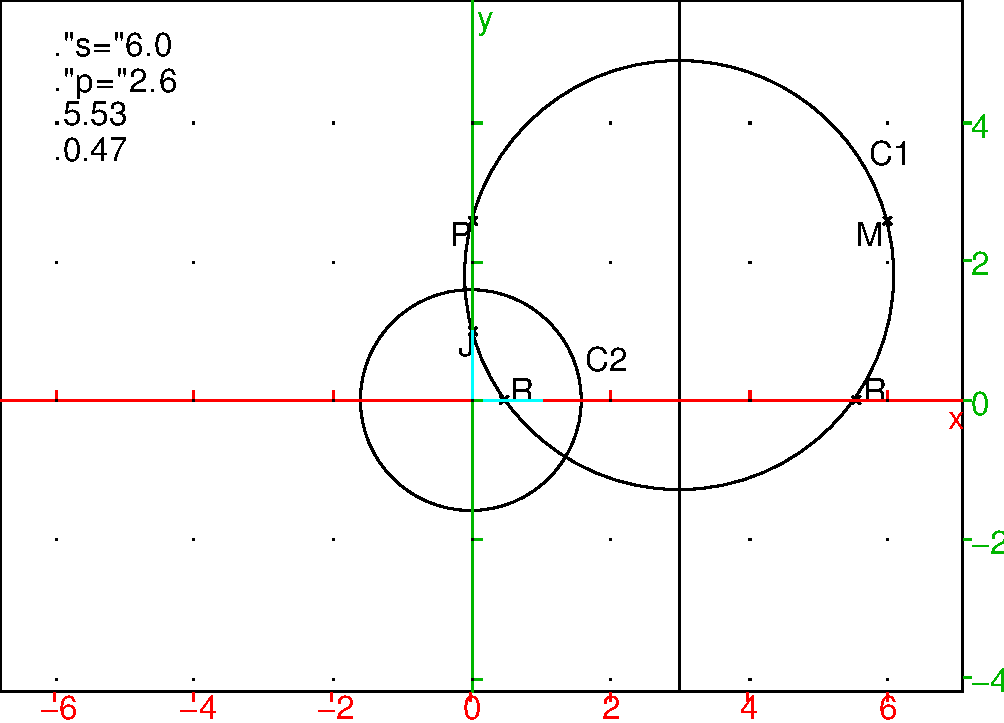
\includegraphics[width=\textwidth]{visutri}\end{center}
\item Si le cercle $C1$ ne coupe pas l'axe $x$, c'est que $s^2-4p< 0$ donc 
  $p\geq 0$ et le cercle $C2$ coupe la droite 
  verticale $x=s/2$ en 2 points qui ont pour affixes les racines de 
  $x^2-sx+p$.\\  
  $C2$ est le cercle d'\'equation $x^2+y^2=p$ (car $s^2-4p< 0$ donc $p\geq 0$) 
  donc les ordonn\'ees $y$ de l'intersection avec $x=s/2$ sont les solutions de 
  $4y^2=4p-s^2$.\\
  Ces 2 points d'intersection ont donc pour affixes les racines de $x^2-sx+p$.
  \begin{center}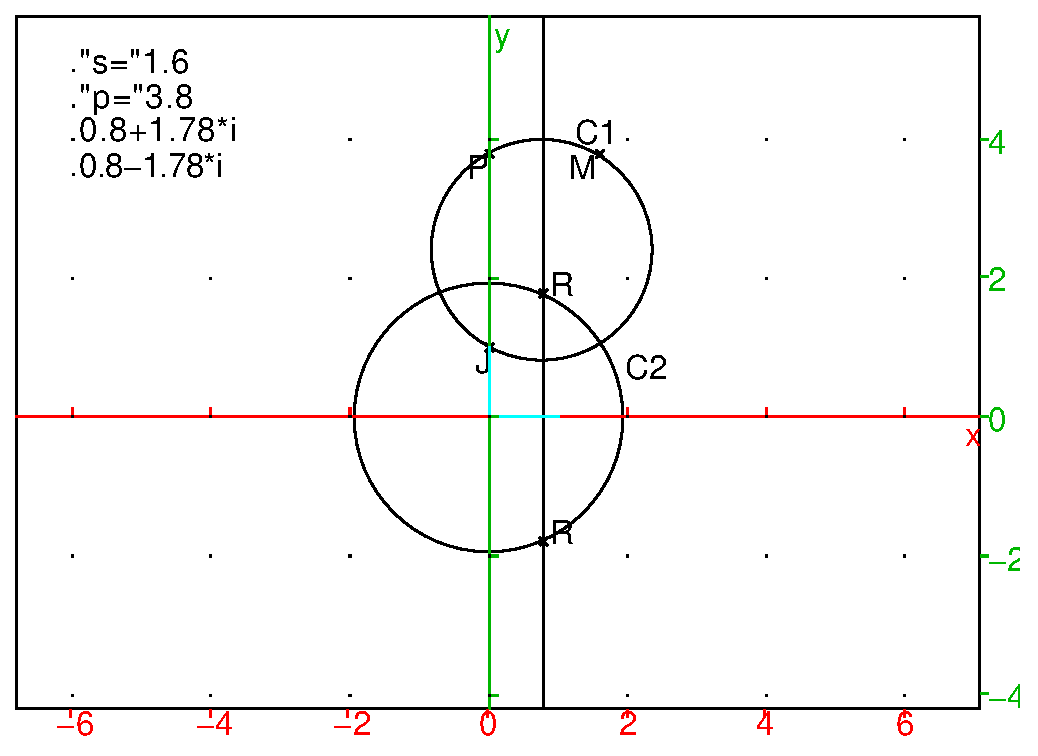
\includegraphics[width=\textwidth]{visutri1}\end{center}
\end{itemize}
Avec {\tt Xcas}, on tape dans un niveau de g\'eom\'etrie :
\begin{verbatim}
assume(s=3);
assume(p=2);
J:=point(i);
P:=point(p*i);
M:=point(s+i*p);
C1:=circonscrit(J,P,M);
C2:=cercle(0,sqrt(abs(p)));
d:=droite(x=s/2):;d;
si s^2-4p>=0 alors R:=inter(C1,droite(y=0)):; 
sinon R:=inter(C2,d):; fsi;
a:=evalf(affixe(R[0]));
b:=evalf(affixe(R[1]));
legende(-6+4*i,a);
legende(-6+3.5*i,b);
legende(-6+5*i,string("s=")+evalf(s));
legende(-6+4.5*i,string("p=")+evalf(p));
\end{verbatim}
\subsection{Simplification de $\sqrt{A+\sqrt B}$ lorsque $A^2-B$ est un carr\'e parfait}
Montrer que :
$$\sqrt 2\sqrt{A+\sqrt B}=\sqrt{A+\sqrt{A^2-B}}+\sqrt{A-\sqrt{A^2-B}}$$
On tape :\\
{\tt normal(expand((sqrt(A+c)+ sqrt(A-c))\verb|^|2))}\\
On obtient :\\
{\tt sqrt(-4*c\verb|^|2+4*A\verb|^|2)+2*A}\\
On tape :\\
{\tt c:=sqrt(A\verb|^|2-B)}
{\tt normal(sqrt(-4*c\verb|^|2+4*A\verb|^|2)+2*A)}\\
{\tt 2*A+sqrt(4*B)}\\
Donc :\\
$\sqrt{A+\sqrt{A^2-B}}+\sqrt{A-\sqrt{A^2-B}}=\sqrt 2\sqrt{A+\sqrt B}$\\
On tape :\\
{\tt sqrt(5+sqrt(21))}\\
On a $5^2-21=4=2^2$, $5+2=7$ et $5-2=3$\\
On obtient donc :\\
{\tt sqrt(7/2)+sqrt(3/2)}\\
On tape :\\
{\tt sqrt(11+6*sqrt(2))}\\
On a $11^2-72=49=7^2$, $11+7=18$ et $11-7=4$\\
On obtient donc :\\
{\tt 3+sqrt(2)}\\
On tape :\\
{\tt sqrt(11+2*sqrt(30))}\\
On a $11^2-120=1=1^2$, $11+1=12$ et $11-1=10$\\
On obtient donc :\\
{\tt sqrt(6)+sqrt(5)}\\

On peut \'ecrire un petit programme qui prend en entr\'ee {\tt (a,b,s)} pour 
simplifier  {\tt sqrt(a+s*sqrt(b))}.\\
On tape :\\
\begin{verbatim}
reduire2(a,b,s):={
  local c;
  si s==0  alors return sqrt(a);fsi;
  c:=round(sqrt(a^2-b*s^2));
  si c^2==a^2-b*s^2 alors
  si s>0  alors return sqrt((a+c)/2)+sqrt((a-c)/2); 
  sinon 
  return sqrt((a+c)/2)-sqrt((a-c)/2);
  fsi;
  fsi;
  return sqrt(a+s*sqrt(b));
}:;
\end{verbatim}
On tape :\\
{\tt reduire2(18,2,-8)}\\
On obtient :\\
{\tt 4-sqrt(2)}\\
On tape :\\
{\tt reduire2(194320499737857776523212040,
  97160249868928888261606031,19713979797994)}\\
On obtient :\\
{\tt sqrt(97160249868928888261606031)+9856989898997}
ou bien, on tape la fonction {\tt simply} qui doit avoir 
{\tt r=sqrt(a+sqrt(b))} comme param\`etre o\`u {\tt b} est sans facteur carr\'e:
\begin{verbatim}
simply(r):={
  local f,a,b,c,d;
  si sommet(r)=='^' alors
  f:=feuille(r);
  a,d:=feuille(f[0]);
  si type(a)==integer alors
  b:=feuille(d)[0];
  c:=sqrt(a^2-b);
  si (round(c))^2==a^2-b alors 
  retourne sqrt((a+c)/2)+sqrt((a-c)/2) 
  fsi;
  sinon 
  d,a:=feuille(f[0]);
  b:=feuille(d)[0];
  c:=sqrt(a^2-b);
  si (round(c))^2==a^2-b alors 
  retourne sqrt((a+c)/2)+sqrt((a-c)/2) 
  fsi;
  fsi;
  fsi;
  retourne r;
}:;
\end{verbatim}
On tape :\\
{\tt simply(sqrt(9+sqrt(17)))}\\
ou \\
{\tt simply(sqrt(sqrt(17)+9))}\\
On obtient :\\
{\tt (sqrt(34))/2+(sqrt(2))/2}
ou bien,  on tape la fonction {\tt simplyf} qui doit avoir comme param\`etre
{\tt r} de la forme {\tt rsqrt(a+s*sqrt(b))} ou {\tt sqrt(a+sqrt(b))} :
\begin{verbatim}
simplyf(r):={
  local f,a,b,c,d,s,sb;
  si sommet(r)=='^' alors
  f:=feuille(r);
  a,d:=feuille(f[0]);
  si type(a)==integer alors
  f:=feuille(d);
  si f[1]==1/2 alors 
  s:=1;
  b:=f[0];
  sinon
  s,sb:=f;
  si type(s)==integer alors
  b:=feuille(sb)[0];
  sinon
  sb,s:=f;
  b:=feuille(sb)[0];
  fsi;
  fsi;
  c:=sqrt(a^2-s^2*b);
  si (round(c))^2==a^2-s^2*b alors 
  retourne sqrt((a+c)/2)+sqrt((a-c)/2); 
  fsi;
  sinon
  d,a:=feuille(f[0]);
  f:=feuille(d);
  si f[1]==1/2 alors 
  b:=f[0];
  s:=1;
  sinon
  s,sb:=f;
  si type(s)==integer alors
  b:=feuille(sb)[0];
  sinon
  sb,s:=f;
  b:=feuille(sb)[0];
  fsi;
  fsi;
  c:=sqrt(a^2-s^2*b);
  si (round(c))^2==a^2-s^2*b alors 
  retourne sqrt((a+c)/2)+sqrt((a-c)/2) 
  fsi;
  fsi;
  fsi;
  retourne r;
}:;
\end{verbatim}
On tape (car {\tt Xcas} remplace {\tt sqrt(128)} par {\tt 8*sqrt(2)}:\\
{\tt simplyf(sqrt(18+sqrt(128)))}\\
ou \\
{\tt simplyf(sqrt(sqrt(128)+18))}\\
ou \\
{\tt simplyf(sqrt(8*sqrt(2)+18))}\\
ou \\
{\tt simplyf(sqrt(18+8*sqrt(2)))}\\
ou \\
{\tt simplyf(sqrt(sqrt(2)*8+18))}\\
ou \\
{\tt simplyf(sqrt(18+sqrt(2)*8))}\\
On obtient :\\
{\tt 4+sqrt(2)}
On tape :\\
{\tt simplyf(sqrt(194320499737857776523212040+19713979797994*sqrt(97160249868928888261606031)))}\\
On obtient :\\
{\tt sqrt(97160249868928888261606031)+9856989898997}
\subsection{Les formules de Cardan}
Les formules de Cardan permettent de r\'esoudre les \'equations de la forme :
$x^3+px+q=0$.\\
Pour cela, on pose $x=u+v$ avec $uv=-p/3$ on a donc \`a r\'esoudre :\\
$x^3+px+q=u^3+v^3+3uv(u+v)+p(u+v)+q=u^3+v^3+q=0$.\\
et on doit r\'esoudre :\\
$u^3+v^3+q=0$ et $u^3v^3=-p^3/27$
On a donc $U=u^3$ et $V=v^3$ qui sont les solutions de l'\'equation du 2-i\`eme 
degr\'e :\\
$X^2+qX-p^3/27=0$ donc \\
\begin{itemize}
\item Si $4p^3+27q^2 \geq 0$ on a :\\
$U=\frac{-q+\sqrt{q^2+4p^3/27}}{2}$ et\\
$V=\frac{-q-\sqrt{q^2+4p^3/27}}{2}$\\
On tape :\\
{\tt solve(x\verb|^|3-6*x-9)}\\
On obtient :\\
{\tt [3,1/2*(-3+(i)*sqrt(3)),1/2*(-3-(i)*sqrt(3))]}\\
En effet $p=-6, q=-9$ donc \\
$4p^3/27+q^2=49$\\
$X^2-9X-(-6)^3/27=X^2-9X+8=(X-1)(X-8)$
0n a donc :
$u=U^{1/3}=8^{1/3}=2$ et $v=V^{1/3}=1$
donc $x=u+v=3$ est solution et on a :\\
$x^3-6*x-9=(x-3)(x^2+3x+3)$
\item Si $4p^3+27q^2 <0$ on a :\\
$u^3=U=\frac{-q+i\sqrt{-q^2-4p^3/27}}{2}$ et\\
$v^3=V=\frac{-q-i\sqrt{-q^2-4p^3/27}}{2}$\\
$arg(u)=-arg(v)=t=arg(U)/3 (\bmod 2\pi/3)$ et $abs(u)=abs(v)=n=abs(U)^{1/3}$\\
Donc :\\
$x_1=u+v=2n\cos(t),\ x_2=u+v=2n\cos(t+2\pi/3),\ x_1=u+v=2n\cos(t+4\pi/3)$\\
avec $n^6=-p^3/27$ soit $n=\sqrt{\frac{-p}{3}}$ et\\ 
$\cos(3t)=-q/2/n^3=\frac{-\frac{q}{2}}{\sqrt{\frac{-p^3}{27}}}$\\
\end{itemize}
\subsection{Simplification de ${(A+\sqrt B)}^{\frac{1}{3}}$} 
Soient :
$u=(A+\sqrt B)^{\frac{1}{3}}$ et $v=(A-\sqrt B)^{\frac{1}{3}}$
On cherche \`a savoir si $u+v$ est un entier.\\
On pose :
$u*v=p$\\
$U=u^3=A+\sqrt B$ et $V=v^3=A-\sqrt B$
On a $U*V=A^2-B=(u*v)^3=p^3$ et\\
$U+V=u^3+v^3=(u+v)(u^2+v^2-uv)=(u+v)((u+v)^2-3uv)=2A$ donc 
$(u+v)^3-3p(u+v)-2A=0$ donc\\
$u+v$ est racine de :\\
$S^3-3pS-2A=0$\\
Pour que ce trin\^ome ait une racine enti\`ere $k$ il faut que $A^2-B$ soit le
cube d'un entier $p$ et que $k$ divise $2*A$ i.e. $k*(k^2-3p)=2*A$.\\

On cherche \`a simplifier :\\
$u=(20+14\sqrt 2)^{1/3}$ et $v=(20-14\sqrt 2)^{1/3}$\\
On a : $A=20,\ B=14^2*2=392 \ 2A=40 \ A^2-B=8=2^3$ donc $p=2$
L'\'equation \`a r\'esoudre est : $S^3-6S=S(S^2-6)=40$\\
Les diviseurs de 40 sont :\\
{\tt idivis(40)}\\
On obtient :
{\tt [1,2,4,8,5,10,20,40]}\\
On tape :
{\tt L:=NULL;for k in  idivis(40) do L:=L,k\verb|^|2-6; end\_for}
On obtient :\\
{\tt -5,-2,10,58,19,94,394,1594}\\
On tape :
{\tt [1,2,4,8,5,10,20,40].*[-5,-2,10,58,19,94,394,1594]}
On obtient :\\
{\tt [-5,-4,40,464,95,940,7880,63760]}
donc $k=4$ est solution et donc :\\
$u=(20+14\sqrt 2)^{1/3}$ et $v=(20-14\sqrt 2)^{1/3}$ sont les racines de 
$X^2-4X+2=0$
On tape :\\
{\tt solve(x\verb|^|2-4x+2)}\\
On obtient :\\
{\tt [-sqrt(2)+2,sqrt(2)+2]}\\
Donc $(20+14\sqrt 2)^{1/3}=2+\sqrt 2$ et $(20-14\sqrt 2)^{1/3}=2-\sqrt 2$.\\
On v\'erifie :\\
On tape :\\
{\tt normal(expand((-sqrt(2)+2)\verb|^|3)),normal(expand((sqrt(2)+2)\verb|^|3))}
On obtient :\\
{\tt -14*sqrt(2)+20,14*sqrt(2)+20}\\

On cherche \`a simplifier :\\
$u=(9+4\sqrt 5)^{1/3}$ et $v=(9-4\sqrt 5)^{1/3}$\\
On a : $A=9,\ B=4^2*5=80 \ 2A=18 \ A^2-B=1=1^3$ donc $p=1$\\
L'\'equation \`a r\'esoudre est : $S^3-3S=S(S^2-3)=18$\\
Les diviseurs de 8 sont :\\
{\tt idivis(18)}\\
On obtient :
{\tt [1,2,3,6,9,18]}\\
On tape :
{\tt L:=NULL;for k in  idivis(18) do L:=L,k\verb|^|2-3; end\_for}\\
On obtient :\\
{\tt -2,1,6,33,78,321}\\
On tape  en utilisant {\tt .*} :\\
{\tt [1,2,3,6,9,18].*[L]}\\
On obtient :\\
{\tt [-2,2,18,198,702,5778]}\\
alors que {\tt [1,2,3,6,9,18]*[L]} renvoie {\tt 6696}\\
donc $k=3$ est solution et donc :\\
$u=(9+4\sqrt 5)^{1/3}$ et $v=(9-4\sqrt 5)^{1/3}$ sont les racines de 
$X^2-3X+1=0$\\
On tape :\\
{\tt solve(x\verb|^|2-3x+1)}\\
On obtient :\\
{\tt [1/2*(3-sqrt(5)),1/2*(3+sqrt(5))]}\\
Donc $(9+4\sqrt 5)^{1/3}=(3+\sqrt 5)/2$ et $(20-14\sqrt 2)^{1/3}=(3-\sqrt 5)/2$.\\
On v\'erifie :\\
On tape :\\
{\tt normal(expand((-sqrt(5)/2+3/2)\verb|^|3)),normal(expand((+sqrt(5)/2+3/2)\verb|^|3))}
On obtient :\\
{\tt -4*sqrt(5)+9,4*sqrt(5)+9}\\
{\bf Remarque} La m\'ethode utilis\'ee ci-dessus n'est valable que lorsque le 
nombre pour lequel on cherche les diviseurs est petit ! Il est donc 
pr\'ef\'erable de faire \'evaluer par {\tt Xcas} {\tt u+v} puis de v\'erifier 
si {\tt u+v} est entier.\\
On peut \'ecrire un petit programme qui prend en entr\'ee {\tt (a,b,s)} pour 
simplifier  {\tt (a+s*sqrt(b))\verb|^|(1/3)}.\\
On \'evite la d\'ecomposition en facteurs premiers trop longue en utilisant 
des {\tt round}.\\
On utilise la fonction {\tt surd} qui est la puisance $1/n$ par exemple :\\
si {\tt a>0}, {\tt surd(a,3)}  renvoie {\tt a\verb|^|(1/3)} et
si {\tt a<0}, {\tt surd(a,3)}renvoie {\tt -(-a)\verb|^|(1/3)}\\
On tape :\\
\begin{verbatim}
reduire3(a,b,s):={
  local c,d,r;
  si s==0  alors return a^(1/3);fsi;
  c:=round(surd(a^2-b*s^2,3));
  d:=round(surd(a+sqrt(b*s^2),3)+surd(a-sqrt(b*s^2),3));
  si (c^3==a^2-b*s^2) alors
  si (d*(d^2-3*c)==2*a) alors
  r:=solve(x^2-d*x+c);
  si s>0 alors return r[1]; else return r[0]; fsi;;
  fsi;
  fsi;
  return (a+s*sqrt(b))^(1/3);
}:;
\end{verbatim}
On tape  :\\
{\tt reduire3(9,5,-4)}\\
On obtient :\\
{\tt 1/2*(3-sqrt(5))}\\
On tape  :\\
{\tt reduire3(747,5,428)}\\
On obtient :\\
{\tt 4*sqrt(5)+3}\\
On tape (avec {\tt Digits:=30}) :\\
{\tt reduire3(957707601542343957074807589821177843432,
  9716024986949,291480749606796380809804976)}\\
On obtient :\\
{\tt sqrt(9716024986949)+9856989898997}
\subsection{Exercices divers de r\'esolution d\'equations}
{\bf R\'esoudre :}
\begin{itemize}
\item $x^2+2x+2=0$\\
On tape :\\
{\tt csolve(x\verb|^|2+2x+2=0)}\\
Ou on tape si on a coch\'e {\tt Complexe} dans la configuration du CAS :\\
{\tt solve(x\verb|^|2+2x+2=0)}\\
On obtient :\\
{\tt [-1-i,-1+i]}
\item $x^4-6x^2+6=0$\\
On tape :\\
{\tt solve(x\verb|^|4-6x\verb|^|2+6=0)}\\
On obtient si on a coch\'e {\tt Sqrt} dans la configuration du CAS :\\
{\tt [-(sqrt(sqrt(3)+3)),-(sqrt(-(sqrt(3))+3)),\\
sqrt(-(sqrt(3))+3),sqrt(sqrt(3)+3)]}
\item $x^6-26x^5+250x^4-1160x^3+2749x^2-134x+1320=0$\\
On tape :\\
{\tt solve(x\verb|^|6-26x\verb|^|5+250x\verb|^|4-1160x\verb|^|3+2749x\verb|^|2-3134x+1320=0)}\\
On obtient :\\
{\tt [1,2,3,4,5,11]}
\item $x^4-ax^3-6x^2+6ax^2+11x^2-11ax-6x+6=0$\\
On tape :\\
{\tt  solve(x\verb|^|4-a*x\verb|^|3-6*x\verb|^|3+6a*x\verb|^|2+11x\verb|^|2-11a*x-6x+6a=0)}\\
On obtient :\\
{\tt [3,2,1,a]}
\item $x^4-\pi x^3-6x^2+6\pi x^2+11x^2-11\pi x-6x+6=0$\\
On tape :\\
{\tt solve(x\verb|^|4-pi*x\verb|^|3-6*x\verb|^|3+6*pi*x\verb|^|2+11x\verb|^|2-11*pi*x-6x+6*pi=0)}\\
On obtient :\\
{\tt [3,2,1,pi]}
\item $x^5-3x-1=0$\\
On tape :\\
{\tt solve(x\verb|^|5-3x-1=0)}\\
On obtient :\\
Attention! Extension algébrique non implémentée pour les poly [1,0,0,0,-3,-1]\\
{\tt [-1.2146480427,0.8029510011728015413e-1+1.328355109820654077*i,\\
0.8029510011728015413e-1-1.328355109820654077*i,\\
-0.3347341419433526871,1.388791984407254183]}
\item $4\sin(x)^2\cos(x)^2+\cos(2x)^2=1$\\
On simplifie, on tape :\\
{\tt simplify(4*sin(x)\verb|^|2*cos(x)\verb|^|2+cos(2x)\verb|^|2-1)}\\
On obtient :\\
{\tt 0}\\
On r\'esoud, on tape :\\
{\tt solve(4*sin(x)\verb|^|2*cos(x)\verb|^|2+cos(2x)\verb|^|2=1)}\\
On obtient si {\tt All\_trig\_sol} est coch\'e ou pas coch\'e dans la configuration du CAS :\\
{\tt [x]}
\item $4\cos(x)^3-3\cos(x)-\sin(2x)-\cos(3x)=0$\\
On simplifie, on tape :\\
{\tt simplify(4*cos(x)\verb|^|3-3*cos(x)-sin(2x)-cos(3x))}\\
On obtient :\\
{\tt -2*cos(x)*sin(x)}
On r\'esoud, on tape :\\
{\tt solve(4*cos(x)\verb|^|3-3*cos(x)-sin(2x)-cos(3x)=0)}\\
On obtient si {\tt All\_trig\_sol} n'est pas coch\'e dans la configuration du CAS :\\
{\tt [0,pi/2,-pi/2,pi]}\\
On obtient si on a coch\'e {\tt All\_trig\_sol} dans la configuration du CAS :\\
{\tt [2*n\_0*pi,(4*n\_1*pi+pi)/2,(4*n\_2*pi-pi)/2,2*n\_3*pi+pi]}
\item $4\cos(x)\cos(2x)\cos(3x)=1$\\
On tape :\\
{\tt solve(4*cos(x)*cos(2x)*cos(3x)=1)}\\
On obtient si {\tt All\_trig\_sol} n'est pas coch\'e dans la configuration du CAS :\\
{\tt [pi/3,-pi/3,2*pi/3,-2*pi/3,pi/8,-pi/8,7*pi/8,-7*pi/8,\\
3*pi/8,-3*pi/8,5*pi/8,-5*pi/8]}\\
On obtient si on a coch\'e {\tt All\_trig\_sol} dans la configuration du CAS :\\
{\tt [(6*n\_6*pi+pi)/3,(6*n\_6*pi-pi)/3,(6*n\_7*pi+2*pi)/3,\\
(6*n\_7*pi-2*pi)/3,(16*n\_8*pi+pi)/8,(16*n\_8*pi-pi)/8,\\
(16*n\_9*pi+7*pi)/8,(16*n\_9*pi-7*pi)/8,(16*n\_10*pi+3*pi)/8,\\
(16*n\_10*pi-3*pi)/8,(16*n\_11*pi+5*pi)/8,(16*n\_11*pi-5*pi)/8]}
\item le syst\`eme lin\'eaire :\\
$[x+2y+3z=1,x+3y+2z=1,3x+y+2z=1]$\\
On tape :\\
{\tt linsolve([x+2y+3z=1,x+3y+2z=1,3x+y+2z=1],[x,y,z])}\\
On obtient :\\
{\tt [1/6,1/6,1/6]}
\item le syst\`eme lin\'eaire :\\
$[x+2y+3z=\pi+5,2x+3y+2z=2\pi+5,3x+\pi y+\pi z=5\pi]$\\
On tape :\\
{\tt linsolve([x+2y+3z=pi+5,2x+3y+2z=2*pi+5,3x+pi*y+pi*z=5*pi],[x,y,z])}\\
On obtient :\\
{\tt [pi,1,1]}
\end{itemize}

\chapter{\'Etude de fonctions}
\section{Exercice : \'etude de $\displaystyle f(x)=\frac{2x^2-1}{6x^2+x-2}$}
\begin{enumerate}
\item Domaine de d\'efinition\\
On tape :\\
{\tt solve(6x\verb|^|2+x-2)}\\
On obtient :\\
{\tt [(-2)/3,1/2]}\\
Donc $f$ est d\'efinie sur $\R-\{-2/3,1/2\}$
\item D\'eriv\'ee\\
On tape :\\
{\tt factor(diff((2x\verb|^|2-1)/(6x\verb|^|2+x-2))}\\
On obtient :\\
{\tt (2*x\verb|^|+4*x+1)/((2*x-1)\verb|^|2*(3*x+2)\verb|^|2)}\\
On tape :\\
{\tt normal(solve(2*x\verb|^|+4*x+1))}\\
On obtient :\\
{\tt [(-sqrt(2)-2)/2,(sqrt(2)-2)/2]}\\
On tape :\\
{\tt evalf([(-sqrt(2)-2)/2,(sqrt(2)-2)/2])}\\
On obtient :\\
{\tt [-1.70710678119,-0.292893218813]}\\
On tape :\\
{\tt subst((2x\verb|^|2-1)/(6x\verb|^|2+x-2),x=-1.70710678119)}\\
On obtient :\\
{\tt 0.35044026276}\\
On tape :\\
{\tt subst((2x\verb|^|2-1)/(6x\verb|^|2+x-2),x=-0.292893218813)}\\
On obtient :\\
{\tt 0.465886267852}\\
$f$ a donc deux extremum en $\simeq$ (-1.71,0.35) et (-0.29,0.47)\\
Donc $f$ est :\\
croissante sur $]-\infty;(-\sqrt 2-2)/2]$\\
d\'ecroissante sur $[(-\sqrt 2-2)/2; -2/3[$\\
d\'ecroissante sur $]-2/3;(\sqrt 2-2)/2]$\\
croissante sur $[(\sqrt 2-2)/;1/2[$\\
croissante sur $]1/2;+\infty[$

\item Branches infinies\\
On tape :\\
{\tt limit((2x\verb|^|2-1)/(6x\verb|^|2+x-2),x=inf)}\\
On obtient :\\
{\tt 1/3}\\
On tape :\\
{\tt limit((2x\verb|^|2-1)/(6x\verb|^|2+x-2),x=-inf)}\\
On obtient :\\
{\tt 1/3}\\
Donc $\displaystyle y=\frac{1}{3}$ est asymptote.\\
On tape :\\
{\tt limit((2x\verb|^|2-1)/(6x\verb|^|2+x-2),x=-2/3,-1)}\\
On obtient :\\
{\tt -infinity}\\
On tape :\\
{\tt limit((2x\verb|^|2-1)/(6x\verb|^|2+x-2),x=-2/3,1)}\\
On obtient :\\
{\tt +(infinity)}\\
Donc $\displaystyle x=\frac{-2}{3}$ est asymptote.\\
On tape :\\
{\tt limit((2x\verb|^|2-1)/(6x\verb|^|2+x-2),x=1/2,-1)}\\
On obtient :\\
{\tt +infinity}\\
On tape :\\
{\tt limit((2x\verb|^|2-1)/(6x\verb|^|2+x-2),x=1/2,1)}\\
On obtient :\\
{\tt -infinity}\\
Donc $\displaystyle x=\frac{1}{2}$ est asymptote.
\item Graphe\\
On tape :\\
{\tt plotfunc((2x\verb|^|2-1)/(6x\verb|^|2+x-2),x=-8..8),}\\
{\tt affichage(droite(x=1/2),droite(x=-2/3),droite(y=1/3),1)}\\
On obtient :\\
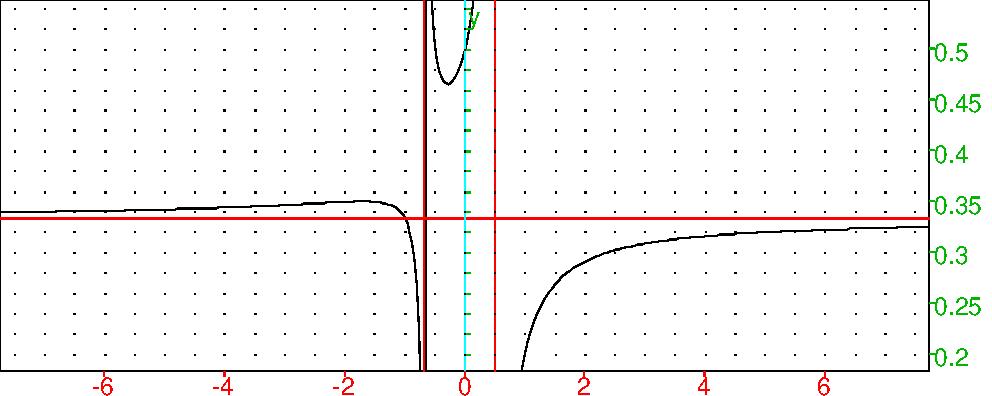
\includegraphics[width=\textwidth]{graphexo}
\end{enumerate}
\section{Exercice : \'etude de $\displaystyle f(x)=\acos(\sin(x))+\asin(\cos(x))$}
%asin1
\begin{enumerate}
\item Domaine de d\'efinition et p\'eriode.\\
\item Montrer que :\\
$f(x+\pi)=f(\pi/2-x)=\pi-f(x)$.
\item Graphe de $f$ et pr\'eciser son centre de sym\'etrie et son axe de sym\'etrie.
\item Valeur de $f(x)$ sur $[0,\pi/2]$ et sur $\pi/2,\pi]$.
\end{enumerate}

{\bf Rappels}\\
On a :\\
$\sin(x)=\cos(\pi/2-x)$\\
$\cos(x)=\sin(\pi/2-x)$\\
$\sin(x+\pi)=-\sin(x)$\\
$\cos(x+pi)=-\cos(x)$\\
$\asin(x)$ est une bijection  de [-1,1] sur $[-\pi/2,\pi/2]$
$\sin(\asin(x))=x$  et \\
si $x\in [-\pi/2,\pi/2]$ alors $\asin(\sin(x))=x$\\
$\acos(x)$ est une bijection  de [-1,1] sur $[0,\pi]$
$\cos(\acos(x))=x$ et \\
si $x\in [0,\pi]$ alors $\acos(\cos(x))=x$\\
$\asin(-x)=-\asin(x)$\\
$\acos(-x)=\pi-\acos(x)$\\
$\asin(x)+\acos(x)=\pi/2$\\
$\asin(x)'=1/\sqrt(1-x^2)$\\
$\acos(x)'=-1/\sqrt(1-x^2)$\\

{\bf La solution avec {\tt Xcas}}
On tape :\\
{\tt f(x):=acos(sin(x))+asin(cos(x))}\\
donc \\
{\tt f(x):=acos(cos(pi/2-x))+asin(sin(pi/2-x))}\\
\begin{enumerate}
\item $f(x+\pi)=f(\pi/2-x)=\pi-f(x)$.\\
On tape :\\
{\tt simplify(f(x+pi)+f(x))}\\
On obtient :\\
{\tt pi}\\
En effet :\\
{\tt f(x+pi)=acos(-sin(x))+asin(-cos(x))}\\
et on a : \\
$\acos(-\sin(x))=\pi-\acos(\sin(x))$\\
$\asin(-\cos(x))=-\asin(\cos(x))$\\
D'o\`u le r\`esultat.\\
On tape :\\
{\tt simplify(f(pi/2-x)+f(x))}\\
On obtient :\\
{\tt pi}\\
En effet :\\
{\tt f(pi/2-x)=acos(cos(x))+asin(sin(x))}\\
et on a : \\
$\acos(\sin(x))+\asin(\sin(x)=\pi/2$\\
$\asin(\cos(x))+\acos(\cos(x))=\pi/2$\\
D'o\`u le r\`esultat.

\item Graphe de $f$.\\
On tape :\\
{\tt f(x):=acos(sin(x))+asin(cos(x))}\\
{\tt plotfunc(f(x))}\\
On obtient :\\
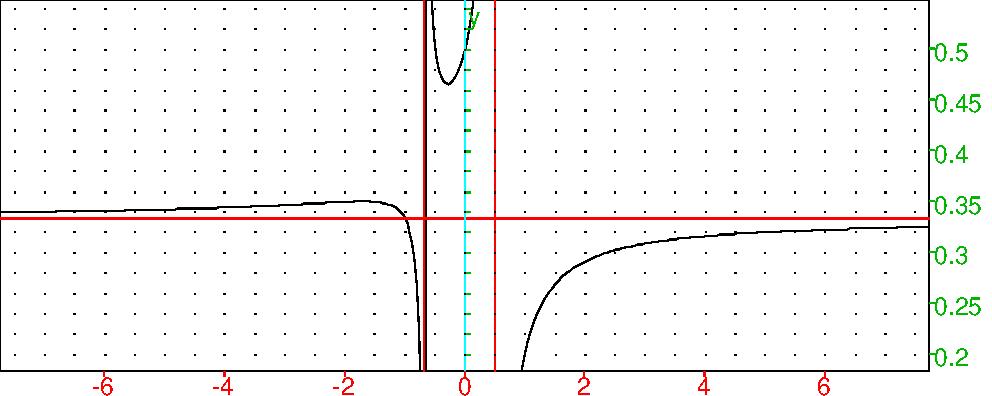
\includegraphics[width=\textwidth]{graphexo}
Le point $S(\pi/4,\pi/2$ est un centre de sym\'etrie car 
on a  $f(x)+f(pi/2-x)=\pi$ donc les points $A(x,f(x)$ et $B(\pi/2-x,f(\pi/2-x)$
sont 2 points de la courbe qui sont sym\'etriques par rapport \`a $S$.\\
En effet $1/2*(x+\pi/2-x)=\pi/4$ et 
$1/2*(f(x)+f(\pi/2-x))=\pi/2$.\\
La droite d'\'equation $x=3\pi/4$ est un axe de sym\'etrie de la courbe.\\
  En effet $f(x+\pi)=f(\pi/2-x)$ et donc les points
$C(x+\pi,f(x+\pi)$ et $D(\pi/2-x,f(\pi/2-x)$ sont sym\'etriques par rapport \`a la droite  $x=3\pi/4$
puisque $1/2*(x+\pi+\pi/2-x)=3\pi/4$

\item Valeur de $f(x)$ sur $[0,\pi/2]$ et sur $\pi/2,\pi]$.
On tape :\\
{\tt assume(x>0 and x<pi/2)}\\
{\tt simplify(f(x))}\\
On obtient :\\
{\tt pi-2*x}\\
Si $x\in [0,\pi/2]$ on a $\pi/2-x\in [0,\pi/2]$ donc
$f(x):=\acos(\cos(\pi/2-x))+\asin(\sin(\pi/2-x))=\pi-2x$
On tape :\\
{\tt assume(x>=pi/2 and x<=pi)}\\
{\tt simplify(f(x))}\\
On obtient :\\
{\tt 0}\\
Si $x\in [\pi/2,\pi]$ on a $x-\pi/2\in [0,\pi/2]$ donc
$f(x):=\acos(\cos(\pi/2-x))+\asin(\sin(\pi/2-x))=$\\
$\acos(\cos(x-\pi/2))-\asin(\sin(x-\pi/2-))=x-\pi/2-(x-\pi/2)=0$

\end{enumerate}





\chapter{Fonctions et \'equations en terminale scientifique}
\section{\'Etude de $\displaystyle f(x)=\ln(\frac{x^2-4x+3}{1-x^2})$}
\begin{enumerate}
\item Domaine de d\'efinition\\
On tape :\\
{\tt solve(x\verb|^|2-4x+3)}\\
On obtient :\\
{\tt [1,3]}\\
On tape :\\
{\tt solve(x\verb|^|2-1)}\\
On obtient :\\
{\tt [-1,1]}\\
On tape :\\
{\tt normal((x\verb|^|2-4x+3)/(1-x\verb|^|2))}\\
On obtient :\\
{\tt (-x+3)/(x+1)}\\
On tape :\\
{\tt solve((x\verb|^|2-4x+3)*(1-x\verb|^|2)>0)}\\
On obtient :\\
{\tt [((x>-1) \&\& (x<1)),((x>1) \&\& (x<3))]}\\
Donc $f$ est d\'efinie sur $]-1;1[\cup]1;3[$
Mais on peut prolonger $f$ par continuit\'e en $1$ en posant $f(1)=\ln(1)=0$
\item D\'eriv\'ee\\
On tape :\\
{\tt factor(diff(ln((x\verb|^|2-4x+3)/(1-x\verb|^|2))))}\\
On obtient :\\
{\tt 4/((x-3)*(x+1))}\\
Or $(x-3)*(x+1)<0$ sur  $]-1; 3[$ donc $f$ est :\\
d\'ecroissante sur $]-1; 3[$\\
On cherche si $f$ est d\'erivable en $x=1$, on tape :\\
{\tt limit(ln((x\verb|^|2-4x+3)/(1-x\verb|^|2))/(x-1),x=1)}\\
On obtient :\\
{\tt -1}\\
Donc $f$ est d\'erivable en $x=1$ et sa d\'eriv\'ee vaut -1.
\item Branches infinies\\
On tape :\\
{\tt limit(ln((x\verb|^|2-4x+3)/(1-x\verb|^|2)),x=-1,1)}\\
On obtient :\\
{\tt +ininity}\\
On tape :\\
{\tt limit(ln((x\verb|^|2-4x+3)/(1-x\verb|^|2)),x=3,-1)}\\
On obtient :\\
{\tt -ininity}\\
Donc $x=-1$ et $x=3$ sont asymptotes.\\
On tape :\\
{\tt limit((2x\verb|^|2-1)/(6x\verb|^|2+x-2),x=-2/3,-1)}\\
On obtient :\\
{\tt -infinity}\\
\item Graphe\\
On tape :\\
{\tt plotfunc(ln((x\verb|^|2-4x+3)/(1-x\verb|^|2)))}\\
{\tt affichage(droite(x=-1),droite(x=3),1),
affichage(droite(y=-x+1),2)}\\
On obtient :\\
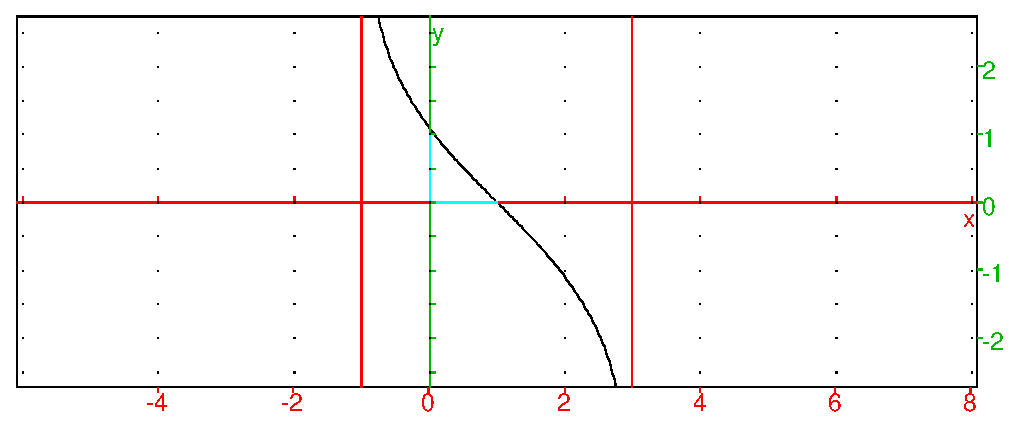
\includegraphics[width=\textwidth]{graphexo1}
\end{enumerate}


\section{Calcul de d\'eriv\'ee n-i\`eme}
\subsection{D\'eriv\'ee n-i\`eme de $\cos(x)^3+\sin(x)^3$}
Calculer la deriv\'ee n-i\`eme de la fonction $f(x)=\cos(x)^3+\sin(x)^3$ en 
fonction de $n$.\\
On va faire cet exercice de deux fa\c{c}ons :
\begin{itemize}
\item On fait le calcul directement en cherchant les relations de r\'ecurrence
entre la d\'eriv\'ee $n-i\`eme$ et la d\'eriv\'ee $(n+1)-i\`eme$ en s'aidant de
 {\tt Xcas}.
\item On lin\'earise $f(x)$ puis on d\'erive.
\end{itemize}
\begin{itemize}
\item On tape :\\
{\tt f(x):=cos(x)\verb|^|3+sin(x)\verb|^|3}\\
{\tt diff(f(x))}\\
On obtient :\\
{\tt -3*cos(x)\verb|^|2*sin(x)+3*cos(x)*sin(x)\verb|^|2}\\
On tape :\\
{\tt diff(f(x),x,2)}\\
On obtient :\\
{\tt -3*cos(x)\verb|^|3-3*sin(x)\verb|^|3+6*cos(x)\verb|^|2*sin(x)+6*cos(x)*sin(x)\verb|^|2}\\
On tape :\\
{\tt diff(f(x),x,3)}\\
On obtient :\\
{\tt 6*cos(x)\verb|^|3-6*sin(x)\verb|^|3+21*cos(x)\verb|^|2*sin(x)-21*cos(x)*sin(x)\verb|^|2}\\
On tape :\\
{\tt diff(f(x),x,4)}\\
On obtient :\\
{\tt 21*cos(x)\verb|^|3+21*sin(x)\verb|^|3-60*cos(x)\verb|^|2*sin(x)-60*cos(x)*sin(x)\verb|^|2}\\
On tape :\\
{\tt diff(f(x),x,5)}\\
On obtient :\\
{\tt -60*cos(x)\verb|^|3+60*sin(x)\verb|^|3-183*cos(x)\verb|^|2*sin(x)+183*cos(x)*sin(x)\verb|^|2}\\
On suppose que la deriv\'ee n-i\`eme est de la forme :\\
$f(x)^{(n)}=a(n)\cos(x)^3+b(n)\cos(x)^2\sin(x)+c(n)\cos(x)\sin(x)^2+d(n)\sin(x)^3$ 
avec $u(n)=|a(n)|=|d(n)|$ et $v(n)=|b(n)|=|c(n)|$
On a la relation de r\'ecurrence :\\
$u(0)=1$ et $v(0)=0$ 
$u(n+1)=v(n)$ et \\
$v(n+1)=3u(n)+2v(n)$
Les signes de |a(n),b(n),c(n),d(n)| sont les m\^emes modulo 4.\\
On a $a(n)*c(n)=b(n)*d(n)<0$
On d\'efinit les fonctions :\\
{\tt p(n):=ifte(irem(n,4)==0 or irem(n,4)==1,1,-1)}\\
{\tt q(n):=ifte(irem(n,4)==0 or irem(n,4)==3,1,-1)}\\
$q(n)=p(n+1)$ donc la d\'efinition de $q$ est inutile.\\
On a alors :\\
$f(x)^{(n)}=p(n+1)u(n)\cos(x)^3+p(n)u(n)\sin(x)^3-p(n)v(n)\cos(x)^2\sin(x)-p(n+1)v(n)\cos(x)\sin(x)^2$ 
Il reste \`a trouver en fonction de $n$ les valeurs de $u(n)$ et de $v(n)$ en 
fonction de $n$.\\
On tape :\\
{\tt rsolve([u(n)=v(n-1),v(n)=3*u(n-1)+2*v(n-1)],[u(n),v(n)],[u(0)=1,v(0)=0])}\\
On obtient :\\
{\tt [[3\verb|^|(n+1)*1/12+(-1)\verb|^|n*3*1/4,3\verb|^|(n+1)*1/4-(-1)\verb|^|n*3*1/4]]}\\ 
Donc :\\
$f(x)^{(n)}=(p(n+1)\cos(x)^3+p(n)\sin(x)^3)*(3^n*\frac{1}{4}+(-1)^n*\frac{3}{4})-(p(n)\cos(x)^2\sin(x)+p(n+)\cos(x)\sin(x)^2)*(3^(n+1)*\frac{1}{4}-(-1)^n*\frac{3}{4})$
\item Pour lin\'eariser on utilise la formule de Moivre :\\
$(\cos(x)+i*\sin(x))^3=\cos(3x)+i*\sin(3x)$ donc\\
$\cos(x)^3+3*i*(1-\sin(x)^2)*\sin(x)-3*\cos(x)*(1-\cos(x)^2)-i\sin(x)^3=\cos(3x)+i*\sin(3x)$\\
Donc :\\
$4\cos(x)^3=\cos(3x)+3*\cos(x)$\\
$4\sin(x)^3=-\sin(3x)+3\sin(x)$
Ou on tape :\\
{\tt tlin(cos(x)\verb|^|3+sin(x)\verb|^|3)}\\
On obtient :\\
{\tt 3*cos(x)/4+cos(3*x)/4+3*sin(x)/4-sin(3*x)/4}\\
Il reste \`a connaitre la d\'eriv\'ee n-i\`eme de $\cos(x)$ et de $\sin(x)$.\\
On a :\\
$\cos(x)'=-\sin(x)=\cos(x+\pi/2)$ et $\sin(x)'=\cos(x)=\sin(x+\pi/2)$ donc\\
$\cos(x)^{(n)}=\cos(x+n\pi/2)$ et $\sin(x)^{(n)}=\sin(x+n\pi/2)$\\
On en d\'eduit que :\\
$$f(x)^{(n)}=\frac{1}{4}*(3(\cos(x+\frac{n\pi}{2})+\sin(x+\frac{n\pi}{2}))+3^n(\cos(3x+\frac{n\pi}{2})-\sin(3x+\frac{n\pi}{2})))$$ 
\end{itemize}
On v\'erifie :\\
On tape :\\
{\tt k(x,n):=(q(n)*cos(x)\verb|^|3+p(n)*sin(x)\verb|^|3)*(3\verb|^|(n+1)*1/12+(-1)\verb|^|n*3*1/4)-(p(n)*cos(x)\verb|^|2*sin(x)+q(n)*cos(x)*sin(x)\verb|^|2)*(3\verb|^|(n+1)*1/4-(-1)\verb|^|n*3*1/4)}\\
{\tt h(x,n):=1/4*(3(cos(x+n*pi/2)+sin(x+n*pi/2))+3\verb|^|n*(cos(3x+n*pi/2)-sin(3x+n*pi/2)))}\\ 
{\tt simplify(k(x,n)-h(x,n))\$(n=0..15)}\\ 
On obtient :\\
{\tt 0,0,0,0,0,0,0,0,0,0,0,0,0,0,0,0}
\subsection{D\'eriv\'ee n-i\`eme de $\exp(-x^2)$}
On veut calculer la deriv\'ee n-i\`eme de la fonction $f(x)=\exp(-x^2)$ en 
fonction de $n$.\\
\begin{itemize}
\item Montrer que $f(x)^{(n)}=\exp(-x^2)P_n(x)$ o\`u $P_n$ est un polyn\^ome 
r\'eel de degr\'e $n$ ayant pour terme de plus haut degr\'e $a_n=(-2)^n$.
De plus si $n$ est pair $P_n(x)$ est pair et si $n$ est impair $P_n(x)$ est
impair. 
\item Montrer que pour $n\geq 1$ et pour tout $x$ r\'eel on a :\\
$P_{n+1}(x)=-2xP_n(x)-2nP_{n-1}(x)$
\item Montrer que, pour $n\geq \N$, $P_n$ v\'erifie l'\'equation 
diff\'erentielle  $y''-2xy'+2ny=0$.\\
En d\'eduire la valeur $P_n(x)$
%\item \'Etudiez les racines de $P_n(x)$.
\end{itemize}
\begin{itemize}
\item On tape :\\
{\tt f(x):=exp(-x\verb|^|2)}\\
{\tt diff(f(x))}\\
On obtient :\\
{\tt -2*x*exp(-x\verb|^|2)}\\
On tape en d\'ecochant {\tt sqrt} dans la configuration du CAS :\\
{\tt factor(diff(f(x),x,2))}\\
On obtient :\\
{\tt 2*(2*x\verb|^|2-1)*exp(-x\verb|^|2)}\\
On tape en d\'ecochant {\tt sqrt} dans la configuration du CAS :\\
{\tt factor(diff(f(x),x,3))}\\
On obtient :\\
{\tt -4*x*(2*x\verb|^|2-3)*exp(-x\verb|^|2)}\\
On tape en d\'ecochant {\tt sqrt} dans la configuration du CAS :\\
{\tt factor(diff(f(x),x,4))}\\
On obtient :\\
{\tt 4*(4*x\verb|^|4-12*x\verb|^|2+3)*exp(-x\verb|^|2)}\\
On tape en d\'ecochant {\tt sqrt} dans la configuration du CAS :\\
{\tt factor(diff(f(x),x,5))}\\
On obtient :\\
{\tt -8*x*(4*x\verb|^|4-20*x\verb|^|2+15)*exp(-x\verb|^|2)}\\
On a obtenu :\\
$P_0(x)=1$, $P_1(x)=-2x$, $P_2(x)=4x^2-2$, $P_3(x)=-8x^3+12x$,\\
$P_4(x)=16x^4-48x^2+12$, $P_5(x)=-32x^5+160x^3-120x$\\
On fait un raisonnement par r\'ecurrence pour montrer la propri\'et\'e :\\
$f(x)^{(n)}=\exp(-x^2)P_n(x)$ o\`u $P_n$ est un polyn\^ome r\'eel de degr\'e 
$n$ avec $a_n=(-2)^n$.\\
Si $f(x)^{(n)}=\exp(-x^2)P_n(x)$ avec $P_n(x)$ un polyn\^ome de degr\'e $n$ 
alors puisque \\
$f(x)^{(n+1)}=\exp(-x^2)(-2xP_n(x)+P_n(x)')$\\
on a $P_{n+1}(x)=-2xP_n(x)+P_{n}(x)'$ et $P_{n+1}$ est bien un polyn\^ome de 
degr\'e $n+1$ et $a_{n+1}=-2*(-2)^n=(-2)^{n+1}$.\\
La propri\'et\'e est vraie pour $n=0$ et si la propri\'et\'e est vraie pour $n$ 
alors elle est vraie pour $n+1$, donc la propri\'et\'e est vraie pour tout 
entier naturel et on a $P_{n+1}(x)=-2xP_n(x)+P_{n}(x)'$
De plus si $P_n$ est pair (resp impair), $2xP_n(x)$ et$P_{n}(x)'$ sont impairs 
(resp pairs) donc $P_{n+1}(x)$ est impair (resp pair). Comme $P_0(x)=1$ est pair
on en d\'eduit que $P_n(x)$ est pair (resp impair) si $n$ est pair (resp impair).
\item On fait encore un raisonnement par r\'ecurrence pour montrer que :
$P_n(x)'=-2nP_{n-1}(x)$ pour $n\geq 1$.\\
On a :\\
$P_1(x)'=-2=-2*1*1$, $P_2(x)'=8x=-2*2*P_1(x)=8x$\\
La propri\'et\'e est vraie pour $n=1$\\
Si elle est vraie pour $n$ alors :\\
$P_n(x)'=-2nP_{n-1}(x)$ et comme on a d'apr\`es la question 1
$P_{n+1}(x)=-2xP_n(x)+P_{n}(x)'$ on en d\'eduit que :\\
$P_{n+1}(x)=-2xP_n(x)-2nP_{n-1}(x)$ donc\\
$P_{n+1}(x)'=-2P_n(x)-2xP_n(x)'-2nP_{n-1}(x)'=$\\
$-2P_n(x)+4nxP_{n-1}(x)-2nP_{n-1}(x)'=-2P_n(x)-2n(-2xP_{n-1}(x)+P_{n-1}(x))$.\\
On a d'apr\`es la question 1 :\
$-2n(-2xP_{n-1}(x)+P_{n-1}(x))=-2nP_n(x)$ donc\\
$P_{n+1}(x)'=-2P_n(x)-2nP_n(x)=-2(n+1)P_n(x)$
La propri\'et\'e est vraie pour $n=1$ et si la propri\'et\'e est vraie pour 
$n\geq 1$ alors elle est vraie pour $n+1$, donc la propri\'et\'e est vraie pour  tout entier $n\geq 1$.\\
{\bf Remarque}\\
Plut\^ot que faire une r\'ecurrence, on peut aussi utiliser la formule de 
Leibniz pour calculer la d\'eriv\'ee n-i\`eme d'un produit, \`a savoir :\\
$(u*v)^{(n)}=\sum_{k=0}^ncomb(n,k)u^{(k)}*v^{(n-k)}$\\
On a $f'(x)=(-2x)*f(x)$  et comme les d\'eriv\'ees k-i\`eme de $-2x$ sont nulle pour k>1 on a :\\
$((-2x)*f(x))^{(n)}=-2xf^{(n)}(x)+n(-2)*f(x)^{(n-1)}=-2xf^{(n)}(x)-2nf(x)^{(n-1)}$\\
Donc:\\
$-2xf^{(n)}(x)-2nf(x)^{(n-1)}=f(x)^{(n+1)}$\\
et pour $n\geq 1$, $P_{n+1}(x)=-2xP_n(x)-2nP_{n-1}(x)$ 

\item On vient de montrer que pour $n\geq 1$ on a :
$P_n(x)'=-2nP_{n-1}(x)$.\\
En d\'erivant cette \'egalit\'e on obtient :\\
$P_n(x)''=-2nP_{n-1}(x)'$ \\
donc on a les 2 \'equations :\\
$-2nP_{n-1}(x)=P_n(x)'$.\\
$-2nP_{n-1}(x)'=P_n(x)''$
Puisque $P_n(x)=-2xP_{n-1}(x)+P_{n-1}(x)'$ on en d\'eduit que :\\
$2nP_n(x)=2x*(-2nP_{n-1}(x)-(-2nP_{n-1}(x)')=2xP_n(x)')-P_n(x)''$ \\
Donc $P_n(x)''-2xP_n(x)'+2nP_n(x)=0$ ce qui signifie que pour $n\geq 1$
$P_n$ v\'erifie l'\'equation diff\'erentielle $y''-2xy'+2ny=0$.
Pour $n=0$ on a $P_0(x)=1$ donc $P_0$ v\'erifie aussi cette \'equation 
diff\'erentielle.
Si $P_n(x)=\sum_{k=0}^na(k)*x^k$ avec $a_n=(-2)^n$ on a :\\
$P_n(x)'=\sum_{k=0}^nk*a(k)*x^{k-1}$ et\\
$P_n(x)''=\sum_{k=0}^nk*(k-1)*a(k)*x^{k-2}$\\
donc
$\sum_{k=0}^nk*(k-1)*a(k)*x^{k-2}+(2n-2*k)*a(k)*x^k=0$\\
$(\sum_{j=0}^{n-2}((j+2)*(j+1)*a(j+2)+(2n-2*j)*a(j))*x^j)+2a(n-1)x^{n-1}+0=0$\\
on obtient :\\
$a_{n-1}=0$ et\\
$a_j=-a_{j+2}(j+2)(j+1)/(2(n-j))$
On sait que $a(n)n=(-2)^n$ donc :\\
$a(n-2)=-a(n)*n(n-1)/(2*2)$\\
$a(n-4)=-a(n-2)*(n-2)(n-3)/(2*4)$\\
....
$a(n-2j)=-a(n-2j+2)*(n-2j+2)(n-2j+1)/(2*2*j)$\\
Donc en multipliant membre \`a membre :\\
$a(n-2j)=(-1)^ja(n)*n!/((n-2j)!2^{2j}*j!)=(-1)^{n-j}*2^{n-2j}n!/((n-2j)!j!)$\\
Puisque $a_{n-1}=0$ donc $a(n-2j-1)=0$\\
Donc :\\
$P_n(x)=\sum_{j=0}^{iquo(n,2)}a(n-2j)x^{n-2j}$\\
En r\'esum\'e :\\
$P_n(x)=(-1)^n\sum_{k=0}^{iquo(n,2)}(-1)^{k}*\frac{n!}{k!*(n-2k)!}*2^{n-2k}*x^{n-2k}$\\
On v\'erifie:\\
On tape pour calculer $P_4(x)$:\\
{\tt n:=4)}\\
{\tt (-1)\verb|^|n*sum((-1)\verb|^|j*n!/(j!*(n-2j)!)*2\verb|^|(n-2j)*x\verb|^|(n-2j),j=0..2)}\\
On obtient $P_4(x)$ :\\
{\tt 16*x\verb|^|4-48*x\verb|^|2+12}\\
On tape :\\
{\tt n:=4)}\\
{\tt (-1)\verb|^|n*sum((-1)\verb|^|j*n!/(j!*(n-2j)!)*2\verb|^|(n-2j)*x\verb|^|(n-2j),j=0..2)}\\
On obtient $P_5(x)$ :
{\tt -32*x\verb|^|5+160*x\verb|^|3-120*x}
\end{itemize}
\subsection{D\'eriv\'ee n-i\`eme de $g(x)=exp(-1/x^2)$}
Soit $g$ la fonction d\'efinie par :\\
$g(0)=0$ et pour $x\neq 0$, $g(x)=\exp(-1/x^2)$.\\
Montrer que $g$ est ind\'efiniment d\'erivable.
Puis, \`a l'aide de l'exercice pr\'ec\'edent et de l'exercice suivant calculer
la d\'eriv\'ee n-i\`eme de $g(x)$.\\
$g$ est ind\'efiniment d\'erivable sur $\R^*$.\\
On tape :\\
{\tt g(x):=exp(-1/x\verb|^|2)}\\
{\tt diff(g(x),x,n)\$(n=1..3)}\\
{\tt diff(g(x),x,4)}\\
On obtient :\\
{\tt 2*exp(-1/x\verb|^|2)/x\verb|^|3,(4*exp(-1/x\verb|^|2)-6*x\verb|^|2*exp(-1/x\verb|^|2))/x\verb|^|6,}\\
{\tt (8*exp(-1/x\verb|^|2)-36*x\verb|^|2*exp(-1/x\verb|^|2)+24*x\verb|^|4*exp(-1/x\verb|^|2))/x\verb|^|9}\\
{\tt (16*exp(-1/x\verb|^|2)-144*x\verb|^|2*exp(-1/x\verb|^|2)+300*x\verb|^|4*exp(-1/x\verb|^|2)-120*x\verb|^|6*exp(-1/x\verb|^|2))/x\verb|^|12}\\
Montrons par r\'ecurrence que : 
$$g(x)^{(n)}=\frac{Q_n(x)}{x^{3n}}*exp(-1/x^2)$$
o\`u $Q_n(x)$ est un polyn\^ome de degr\'e $2(n-1)$.\\
On a d'apr\`es les calculs pr\'ec\'edents :\\
$Q_1(x)=-2$\\
$Q_2(x)=4-6*x^2$\\
$Q_3(x)=8-36*x^2+24*x^4$\\
$Q_4(x)=16-144*x^2+300*x^4-120*x^6$\\
On calcule $g(x)^{(n+1)}$ en fonction de $g(x)^{(n)}$ :\\
si $g(x)^{(n)}=\frac{Q_n(x)}{x^{3n}}*exp(-1/x^2)$ on a \\
$g(x)^{(n+1)}=2\frac{Q_n(x)}{x^{3(n+1)}}*exp(-1/x^2)+\frac{Q_n(x)'}{x^{3n}}*exp(-1/x^2)-\frac{3nQ_n(x)}{x^{3n+1}}*exp(-1/x^2)$\\
Donc :\\
$g(x)^{(n+1)}=\frac{Q_{n+1}(x)}{x^{3(n+1)}}*exp(-1/x^2)$ avec \\
$Q_{n+1}(x)=-2Q_n(x)+x^3Q_n(x)'-3nx^2Q_n(x)=x^3Q_n(x)'+(2-3nx^2)Q_n(x)$
$Q_{n+1}(x)$ est donc bien un polyn\^ome de degr\'e $2+2(n-1)=2n$
Montrons que $g$ est ind\'efiniment d\'erivable en 0 et que $g^{(n)}(0)=0$.\\
On tape :\\
{\tt limite(g(x),x=0)}\\
On obtient :\\
{\tt 0}
$g$ est donc continue en 0.\\
On tape :\\
{\tt limite(g(x)/x,x=0,1)}\\
On obtient :\\
{\tt 0}\\
On tape :\\
{\tt limite(g(x)/x,x=0,1)}\\
On obtient :\\
{\tt 0}\\
$g$ est donc d\'erivable en 0.\\
On a $g^{(n)}/x=\frac{Q_n(x)}{x^{3n+1}}*exp(-1/x^2)$.\\
Donc $\lim_{x->0}g^{(n)}/x=0$\\
On tape :\\
{\tt assume(k,integer)}\\
{\tt limite(g(x)/x\verb|^|k,x=0,1)}\\
On obtient :\\
{\tt 0}\\
On tape :\\
{\tt limite(g(x)/x\verb|^|k,x=0,1)}\\
On obtient :\\
{\tt 0}\\
Donc $g$ est ind\'efiniment d\'erivable en 0 et $g^{(n)}(0)=0$.\\
On a :\\
$x^3*g'(x)=2g(x)$
On d\'erive $n$ fois $x^3*g'(x)$ en utilisant la formule de Leibniz.\\
Les d\'eriv\'ees n-i\`eme de $x^3$ sont nulles pour $n>3$ donc :\\
$2g(x)^{(n)}=(x^3*g'(x))^{(n)}=\sum_{k=0}^3comb(n,k)*(x^3)^{(k)}(g(x))^{(n-k+1)}$\\
donc\\
$2g(x)^{(n)}=x^3g(x)^{(n+1)}+3nx^2g(x)^{(n)}+3n(n-1)xg(x)^{(n-1)}+3n(n-1)(n-2)g(x)^{(n-2)}$\\
On en d\'eduit que :\\
$Q_{n+1}(x)+(3nx^2-2)Q_{n}(x)+3n(n-1)x^4Q_{n-1}(x)+3n(n-1)(n-2)x^6Q_{n-2}(x)=0$\\
Pour d\'eterminer $Q_n(x)$ on va utiliser l'exercice pr\'ec\'edent et
l'exercice qui suit !

\subsection{D\'eriv\'ee n-i\`eme de $g(x)=f(1/x)$}
Soit $f$ une fonction ind\'efiniment d\'erivable.
On cherche \`a exprimer la d\'eriv\'ee n-i\`eme de $g(x)=f(1/x)$ en fonction de la d\'eriv\'ee n-i\`eme de $f$.\\
Puis en utilisant la valeur de la d\'eriv\'ee n-i\`eme de $f(x)=exp(-x^2)$, on 
pourra par exemple trouver les d\'eriv\'ees n-i\`eme de la fonction $g$ d\'efinie par $g(0)=0$ et pour $x\neq 0$, $g(x)=\exp(-1/x^2)$.\\
Pour cela on cherche \`a exprimer la d\'eriv\'ee n-i\`eme de $g(x)=f(1/x)$ en 
fonction de la d\'eriv\'ee n-i\`eme de $f$.\\
On tape :\\
{\tt g(x):=f(1/x)}\\
{\tt diff(g(x),x,n)\$(n=1..3)}\\
On obtient :\\
{\tt -f'(1/x)/x\verb|^|2,(2*f'(1/x)+f''(1/x))/x\verb|^|3,(-6*x\verb|^|2*f'(1/x)-6*x*f''(1/x)-f'''(1/x))/x\verb|^|6}\\
On tape :\\
{\tt diff(g(x),x,4)}\\
On obtient :\\
{\tt (24*x\verb|^|3*f'(1/x)+36*x\verb|^|2*f''(1/x)+12*x*f'''(1/x)+f''''(1/x))/x\verb|^|8}\\
On va montrer que :\\
$g^{(n)}(x)=\sum_{k=1}^na(k,n)x^{-n-k}f^{(k)}(1/x)$
avec 
$a(1,n)=(-1)^nn!$\\
$a(k,n)=\frac{(-1)^nn!(n-1)!}{k!(k-1)!(n-k)!}$\\
$a(n,n)=(-1)^n$\\
On a :\\
$g^{(n+1)}(x)=-\sum_{k=1}^na(k,n)x^{-n-k-2}f^{(k+1)}(1/x)-\sum_{k=1}^na(k,n)(n+k)x^{-n-k-1}f^{(k)}(1/x)$\\
Donc :\\
$a(1,n+1)=-a(1,n)(n+1)$,\\
Comme $a(1,1)=-1$ on en d\'eduit que $a(1,n)=(-1)^nn!$\\
$a(n+1,n+1)=-a(n,n)$,\\
Comme $a(1,1)=-1$ on en d\'eduit que $a(n,n)=(-1)^n$\\
 En  posant j=k-1 dans la 2i\`eme somme:\\
$\sum_{k=1}^na(k,n)(n+k)x^{-n-k-1}f^{(k)}(1/x)=\sum_{j=0}^{n-1}a(j+1,n)n(n+j+1)x^{-n-j-2}f^{(j+1)}(1/x)$\\
Donc pour $k=1..n-1$ :\\
$a(k+1,n+1)=-a(k,n)-a(k+1,n)n(n+k+1)$\\
ou encore $j=k+1$:\\
$a(j,n+1)=-a(j-1,n)-a(j,n)n(n+j)$ pour $j=2..n$\\
Si $a(k,n)=\frac{(-1)^nn!(n-1)!}{k!(k-1)!(n-k)!}$ pour $k=1..n$\\
$a(k,n+1)=-\frac{(-1)^nn!(n-1)!}{(k-2)!(k-1)!(n-k+1)!}+\frac{(-1)^nn!(n-1)!n(n+k)}{k!(k-1)!(n-k)!}$
$a(k,n+1)=\frac{(-1)^{n+1}n!(n-1)!}{(k-2)!(k-1)!(n-k)!}*(\frac{1}{n-k+1}+\frac{n+k}{k(k-1)})$
On tape :\\
{\tt factor(1/(n-k+1)+(n+k)/(k*(k-1)))}\\
On obtient :\\
{\tt n*(n+1)/(k*(k-1)*(n-k+1))}\\
Donc pour $k=2..n$ :\\
$a(k,n+1)=\frac{(-1)^{n+1}n!(n+1)!}{k!(k-1)!(n-k+1)!}$\\
On a donc montr\'e par r\'ecurrence que :\\
$$g^(n)(x)=\sum_{k=1}^n\frac{(-1)^nn!(n-1)!}{k!(k-1)!(n-k)!}x^{-n-k}f^{(k)}(1/x)$$
Si $f(x)=\exp(-x^2)$, on sait que :\\
$f^{(k)}(1/x)=P_k(1/x)*\exp(-1/x^2)$
donc si $g(x)=\exp(-1/x^2)=f(1/x)$, on a :\\
$g^(n)(x)=\sum_{k=1}^n\frac{(-1)^nn!(n-1)!}{k!(k-1)!(n-k)!}x^{-n-k}P_k(1/x)\exp(-1/x^2)$\\
$P_k(x)=(-1)^n\sum_{j=0}^{iquo(k,2)}(-1)^{j}*\frac{k!}{j!*(k-2j)!}*2^{k-2j}*x^{k-2j}$\\
Or $P_k(1/x)=(-1)^n\sum_{j=0}^{iquo(k,2)}(-1)^{j}*\frac{k!}{j!*(k-2j)!}*2^{k-2j}*x^{2j-k}= R_k(x)/x^k$ donc\\
$R_k(x)=(-1)^n\sum_{j=0}^{iquo(k,2)}(-1)^{j}*\frac{k!}{j!*(k-2j)!}*2^{k-2j}*x^{2j}$
\\
$\sum_{j=0}^kc(j,k)x^{k-j}=\sum_{j=0}^kc(k-j,k)x^{j}$\\
donc $x^{-n-k}P_k(1/x)= R_k(x)/x^{n+2k}$.\\

$x^{3n}g^(n)(x)=(\sum_{k=1}^n\frac{(-1)^nn!(n-1)!}{k!(k-1)!(n-k)!}R_k(x)*x^{2*n-2k})\exp(-1/x^2)$\\
Donc :\\
$Q_n(x)=\sum_{k=1}^n\frac{(-1)^nn!(n-1)!}{k!(k-1)!(n-k)!}R_k(x)*x^{2*n-2k}$ avec\\
$R_k(x)=(-1)^n\sum_{j=0}^{iquo(k,2)}(-1)^{j}*\frac{k!}{j!*(k-2j)!}*2^{k-2j}*x^{2j}$
\\
On v\'erifie que :\\
$Q_1(x)=-2$\\
$Q_2(x)=4-6*x^2$\\
$Q_3(x)=8-36*x^2+24*x^4$\\
$Q_4(x)=16-144*x^2+300*x^4-120*x^6$\\
On tape :\\
{\tt R(n,x):=(-1)\verb|^|n*sum((-1)\verb|^|j*n!/(j!*(n-2j)!)*2\verb|^|(n-2j)*x\verb|^|(2j),j=0..iquo(n,2)}\\
{\tt Q(n,x):=sum((-1)\verb|^|n*(n!*(n-1)!)/(k!*(k-1)!*(n-k)!)*R(k,x)*x\verb|^|(2*n-2k),k=1..n)}\\
{\tt Q(3,x)}\\
On obtient :\\
{\tt 24*x\verb|^|4-36*x\verb|^|2+8}\\
On tape :\\
{\tt Q(3,x)}\\
On obtient :\\
{\tt -120*x\verb|^|6+300*x\verb|^|4-144*x\verb|^|2+16}\\
Ouf ! c'est correct!

\chapter{Arithm\'etique en terminale scientifique}
\section{\'Enonc\'e sur la partie enti\`ere}
Montrer que la partie enti\`ere de $a=(3+\sqrt 5)^n$ est un entier impair 
quelque soit l'entier $n$ dans $\mathbb N$. 
\subsection{Cherchons avec {\tt Xcas}}
On peut faire des essais dans le tableur.\\
Dans A0 on met 1\\
Dans A1 on met =A0*(3+sqrt(5))\\ 
Dans B0 on met =floor(A0)\\
Dans B1 on met =floor(B1)\\
Puis on remplit vers le bas.\\
Dans cet exercice il faut penser \`a associer \`a
$(3+\sqrt 5)^n$ sa quantit\'e conjugu\'ee $(3-\sqrt 5)^n$.\\
Dans C0 on met 1\\
Dans C1 on met =C0*(3-sqrt(5))\\ 
Dans D0 on met =floor(A0+C0)\\
Dans D1 on met =C0*(3-sqrt(5))\\ 
Puis on remplit vers le bas.
\subsection{La d\'emonstration}
On remarque que :\\
$b=(3+\sqrt 5)^n+(3-\sqrt 5)^n$ est un entier pair (d'apr\`es la formule du
bin\^ome) et que $0<(3-\sqrt 5)^n<1$.\\
On a donc $a<b<a+1$, ou encore $b-1<a<b$ avec $b$ un entier pair.\\
Cela prouve que la partie enti\`ere de $a=(3+\sqrt 5)^n$ est $b-1$
qui est un entier impair.
\section{\'Enonc\'es sur le nombre de diviseurs d'un entier}
\subsection{L'\'enonc\'e 1}
Quel est, parmi les entiers naturels de 1 \`a 2005, celui qui admet le plus
de diviseurs ? Quel est ce nombre de diviseurs ?
\subsection{R\'eponse avec {\tt Xcas}}
\noindent On tape :\\
{\tt 2*3*5*7}\\
On obtient :\\
{\tt 210}\\
On tape :\\
{\tt 2*3*5*7*11}\\
On obtient :\\
{\tt 2310}\\ 
Cela nous dit que le nombre est de la forme :\\
$2^a*3^b*5^c*7^d$ avec $a \geq b \geq c \geq d \geq 0$\\
et alors son nombre de diviseurs est :\\
$(a+1)(b+1)(c+1)(d+1)$\\
On peut maintenant faire une recherche syst\'ematique :\\
Il semble qu'il faut supposer que  $d \neq 0$ car avec
- $b=0,c=0, d=0$ on ne peut avoir que $2^10$ qui n'a que 11 diviseurs,\\
- $c=0,d=0$ $(a+1)(b+1)$ \\ 
vaut 20 pour $a=9$ et $b=1$ ($2^9*3=1536$)\\
vaut 28 pour $a=6$ et $b=3$ ($2^6*3^3=1728$)\\
- $d=0$ $(a+1)(b+1)(c+1)$ \\
vaut 32 pour $a=7$, $b=1$ et $c=1$ ($2^7*3*5=1920$)\\
vaut 36 pour $a=5$, $b=2$ et $c=1$ ($2^5*3^2*5=1444$)\\
- si $d \neq 0$ \\
On tape :\\
{\tt 210*6}\\
On obtient :\\
{\tt 1260}\\
et 1260 admet 3*3*2*2=36 diviseurs ou on tape :\\
{\tt size(idivis(1260))}\\
On obtient :\\
{\tt 36}\\
On tape :\\
{\tt 210*8}\\
On obtient :\\
{\tt 1680}\\
et 1680 admet 5*2*2*2=40 diviseurs ou on tape :\\
{\tt size(idivis(1680))}\\
On obtient :\\
{\tt 40}\\
On fait une recherche syst\'ematique :\\
$2^{10}=1024$ a 11 diviseurs,\\
$2^9*3=1536$ a 20 diviseurs,\\
$2^7*3^2=1116$ a 24 diviseurs,\\
$2^6*3^3=1728$ a 28 diviseurs,\\
$2^4*3^4=1296$ a 25 diviseurs,\\
$2^7*3*5=1920$ a 32 diviseurs,\\
$2^5*3^2*5=1440$ a 24 diviseurs,\\
$2^4*3*5*7=1680$ a 40 diviseurs.
\subsection{L'\'enonc\'e 2}
\noindent 1/ Trouver le plus petit nombre entier $n$ qui admet exactement 50 
diviseurs.\\
2/ Existe-t-il un entier $m$ qui soit inf\'erieur \`a $n$ et qui admette plus 
de 50 diviseurs ?
\subsection{R\'eponse avec {\tt Xcas}}
\noindent On sait que si $n=a^p*b^q*c^r$ le nombre de diviseurs de $n$ est 
$(p+1)(q+1)(r+1)$.\\
On a :\\
{\tt 50=1*50=2*25=10*5=2*5*5} 
1/ On cherche le plus petit nombre entier qui admet exactement 50 diviseurs, 
donc les candidats sont :\\
$2^{49}$\\
$2^{24}*3$\\
$2^9*3^4$\\
$2^4*3^4*5$\\
C'est donc $6480=2^4*3^4*5$\\
On tape :\\
{\tt size(idivis(6480))}\\
On obtient :\\
{\tt 50}\\
2/ On doit avoir :\\
$m<2^4*3^4*5$ donc pour qu'il est plus que 50 diviseurs il faut que $m$ soit de
la forme $m=2^p*3^q*5^r*7^s$ avec $p<=4,q<4,r=1,s=1$ et $4(p+1)(q+1)>50$.\\
Essayons $p=4,q=2$, on a $4(p+1)(q+1)=60>50$ et $m=2^4*3^2*5*7=5040$.\\
Donc $m=$ r\'epond \`a la question.
\subsection{L'\'enonc\'e 3}
Soit une s\'equence {\tt L} d'objets. On prend 3 objets parmi cette s\'equence
{\tt L}. \'Ecrire un programme {\tt triplets} qui renvoie la s\'equence de 
dimension {\tt comb(size(L),3)} constitu\'ee par les 3 objets obtenus.\\
{\bf Application num\'erique}
{\tt L} est la liste des diviseurs de $n=12$.

Soit un entier {\tt n}. On cherche 3 diviseurs diff\'erents {\tt n1,n2,n3} de 
{\tt n}, tels que {\tt n1+n2+n3} soit aussi un diviseur de {\tt n}.\\
Modifier le programme pr\'ec\'edent en {\tt solutions} pour obtenir toutes les 
solutions.\\
{\bf Application num\'erique}
$n=12$\\
$n=60$\\
$n=6279$\\
On tape :
\begin{verbatim}
triplets(L):={
  local LR,LT,j,k,l,s;
  LR:=NULL;
  LT:=NULL;
  s:=size(L)-1;
  pour j de 0 jusque s-2 faire
    pour k de j+1 jusque s-1 faire
      pour l de k+1 jusque s faire
        LT:=LT,[L[j],L[k],L[l]];
      fpour;
    fpour;
  fpour;
  retourne LT;
}:;
\end{verbatim}
On tape pour $n=12$ :\\
{\tt LT:=triplets(idivis(12));size(LT);comb(3);comb(6,3)}\\
On obtient :\\
{\tt [1,2,3],[1,2,4],[1,2,6],[1,2,12],[1,3,4],[1,3,6],[1,3,12],}\\
{\tt [1,4,6],[1,4,12],[1,6,12],[2,3,4],[2,3,6],[2,3,12],[2,4,6],}\\
{\tt [2,4,12],[2,6,12],[3,4,6],[3,4,12],[3,6,12],[4,6,12],20,20}\\
On tape :
\begin{verbatim}
solutions(n):={
  local LR,LT,L,j,k,l,s;
  LR:=NULL;
  LT:=NULL;
  L:=idivis(n);
  s:=size(L)-1;
  pour j de 0 jusque s-2 faire
    pour k de j+1 jusque s-1 faire
      pour l de k+1 jusque s faire
        LT:=LT,[L[j],L[k],L[l]];
      fpour;
    fpour;
  fpour;
  s:=size(LT)-1;
  pour j de 0 jusque s faire
    si irem(n,sum(LT[j]))==0 alors
      LR:=LR,LT[j];
    fsi;
  fpour;
  retourne LR;
}:;
\end{verbatim}
On tape pour $n=12$ :\\
{\tt LS:=solutions(12);size(LS)}\\
On obtient 2 solutions (sur les 20 triplets):\\
{\tt [1,2,3],[2,4,6],2}\\
On tape pour $n=60$ :\\
{\tt LS:=solutions(60);size(LS)}\\
On obtient 20 solutions (sur les 220 triplets):\\
{\tt [1,2,3],[1,2,12],[1,3,6],[1,4,5],[1,4,10],[1,4,15],[1,5,6],}\\
{\tt [2,3,5],[2,3,10],[2,3,15],[2,4,6],[2,6,12],[3,4,5],[3,5,12],}\\
{\tt [3,12,15],[4,5,6],[4,6,10],[4,6,20],[5,10,15],[10,20,30],20}\\
On tape pour $n=6279$ :\\
{\tt LS:=solutions(6279);size(LS)}\\
On obtient 9 solutions (sur les 560 triplets):\\
{\tt [1,7,13],[1,21,69],[1,69,91],[3,7,13],[3,13,23],[3,23,273],}\\
{\tt [7,23,39],[21,91,161],[23,161,299],9}

\section{\'Enonc\'es sur l'identit\'e de B\'ezout}
\subsection{L'\'enonc\'e 1}
Quel est le plus petit nombre entier avec lequel il faut multiplier 49 pour 
obtenir un nombre se terminant par 999999999 (9 neufs) ?

{\bf R\'eponse niveau primaire}\\
On peut faire une multiplication \`a trous :
$$49*.........=..999999999$$
On trouve :
$$49*693877551=33999999999$$
{\bf R\'eponse niveau coll\`ege}\\
On a $9999999999=10^9-1$ et le r\'esultat de la multiplication doit \^etre de 
la forme $n*10^9+10^9-1$ avec $0\leq n<49$ (ou de la forme $p*10^9-1$)
avec $0< p \leq 49$.\\
On utilise le tableur en cherchant $n$ pour que :
$n*10^9+10^9-1$ soit divisible par 49.\\
On utilisera les commandes {\tt irem(a,b)} et {\tt iquo(a,b)} qui renvoient 
respectivement le reste et le quotient de la division euclidienne de {\tt a} 
par {\tt b}.\\ 
Pour cela on met dans la premi\`ere colonne les nombres de 0 \`a 48, puis dans 
la deuxi\`eme colonne les nombres $n*10^9+10^9-1$ pour $n$ de 0 \`a 48.
Dans la troisi\`eme colonne on calcule le reste de la division de la deuxi\`eme
colonne par 49 et on trouve que pour $n=33$ ce reste est nul.
Il reste \`a calculer {\tt iquo(33*10\verb|^|9+10\verb|^|9-1,49)} et on 
trouve :
$$693877551$$ 
Mais cette m\'ethode est tr\`es couteuse !
On peut aller un peu plus vite (surtout si on veut faire les calculs \`a la 
main) en remarquant que $10=3 \bmod 7$ et que $100=2 \bmod 49$ donc :\\
$10^3=-1 \bmod 7$\\
$10^6=1 \bmod 7$\\
$10^9=-1 \bmod 7$\\
$10^8=2^4=16 \bmod 49$\\
$10^9=13 \bmod 49$\\
$13*-7=7 \bmod 49$\\
On cherche $a$ tel que $a*10^9=49*k+1=7*p+1$.\\
donc $-a=1 \bmod 7$ et $13*a=1 \bmod 49$\\
Si $a=48$ on a $13*a=-13=36 \bmod 49$\\
Si $a=41$ on a $13*a=13*-1+13*-7=-13+7=-6 \bmod 49$\\
Si $a=34$ on a $13*a=13*-1+13*-7+13*-7=1 \bmod 49$\\
Donc $34*10^9=1 \bmod 49$\\
Il reste \`a calculer {\tt iquo(34*10\verb|^|9-1,49)} et on 
trouve :
$$693877551$$ 
{\bf R\'eponse niveau TS}\\
On a : $999999999+1=10^9$.\\
On cherche $p$ pour avoir : $p*49=a*10^9-1$ c'est \`a dire 
$1=a*10^9-p*49$.

Avec {\tt Xcas} on tape :\\
{\tt bezout\_entiers(49,10\verb|^|9)}\\
On obtient :\\
{\tt [306122449,-15,1]}\\
Donc :\\
$49*306122449-15*10^9=1$
et puisque $49*10^9-49*10^9=0$, on a :\\
$49*(10^9-306122449)+(15-49)*10^9=-1$.\\
Puisque $10^9-306122449=693877551$ et $(49-15)=34$, on a :
$$49*693877551=34*10^9-1=33999999999$$
Pour faire les calculs \`a la main on \'ecrit :\\
$10^9=13 \bmod 49$\\
donc on \'ecrit les 2 premi\`eres \'equations :
$$0*13+1*49=49$$
$$1*13+0*49=13$$
puisque $49=3*13+10$ on soustrait 3 fois l'\'equation 2 \`a l'\'equation 1 et
on obtient l'\'equation 3 :
$$-3*13+1*49=10$$
puisque $13=1*10+3$ on soustrait l'\'equation 3 \`a l'\'equation 2 et
on obtient l'\'equation 4 :
$$4*13-1*49=3$$
puisque $10=3*3+1$ on soustrait  3 fois l'\'equation 4 \`a l'\'equation 3 et
on obtient l'idendit\'e de B\'ezout :
$$-15*13+4*49=1$$
On a $-15=34 \bmod 49$ et $10^9=13 \bmod 49$ donc
$34*10^9-1$ est divisible par 49.\\
Il reste \`a calculer {\tt iquo(34*10\verb|^|9-1,49)} et on 
trouve :
$$693877551$$ 
\subsection{L'\'enonc\'e 2}
R\'esoudre en nombres entiers :
$$13x+5y=1$$
$$5x+13y=6$$

Avec {\tt Xcas} on tape :\\
{\tt bezout\_entiers(13,5)}\\
On obtient :\\
{\tt [2,-5,1]}\\
Donc $2*13-5*5=1$.\\
et puisque $k*13*5-k*13*5=0$, on a :
$13*(2+5k)-(5+13k)*5=1$.\\ 
$13x+5y=1$ a donc comme solutions $x=2+5k,y=-5-13k$ avec $k$ dans $\Z$.\\
En multipliant l'\'egalit\'e $13*(2+5k)-(5+13k)*5=1$ par 6 on a :\\
$13*(12+30k)-(30+78k)*5=6$\\
$5x+13y=6$ a donc comme solutions $x=-30-78k,y=12+30k$ avec $k$ dans $\Z$.

\section{\'Enonc\'es sur des nombres de $\Z/p\Z$}
\subsection{L'\'enonc\'e 1}
Trouver les 2 derniers chiffres de $19969^{19969}$.

Ici, on est s\^ur que le dernier chiffre est 9, puisque 19969 est un nombre 
impair.\\
Avec {\tt Xcas}, on tape :\\
{\tt powmod(19969,19969,100)}
On obtient : {\tt 29}\\
On peut aussi taper mais le calcul est inefficace :\\
{\tt irem(19969\verb|^|19969,100)}
\subsection{L'\'enonc\'e 2}
Trouver les 2 derniers chiffres de $19996^{19996}$.

Ici, on est s\^ur que le dernier chiffre est 6.\\
Avec {\tt Xcas}, on tape :\\
{\tt powmod(19996,19996,100)}
On obtient : {\tt 96}\\
On peut aussi taper directement pour v\'erifier :\\
{\tt irem(19996\verb|^|19996,100)}

\section{{\bf TP} sur l'indicatrice d'Euler}
\subsection{L'\'enonc\'e}
{\bf Bijection entre $\Q \cap [0,1]$ et $\N$}\\
On construit une bijection $f$ entre les rationnels de [0,1] et $\N$, 
pour cela :
\begin{itemize}
\item on ordonne les rationnels de [0,1] de la fa\c{c}on suivante :
$$0,1,\frac{1}{2},\frac{1}{3},\frac{2}{3},\frac{1}{4},\frac{2}{4},\frac{3}{4},
...\frac{1}{n}\frac{2}{n}...\frac{n-1}{n},...$$
\item on supprime les fractions non irr\'eductibles et on obtient une suite 
$L$.
\end{itemize}
La fonction $f$ attribue \`a un rationnel de [0,1] son rang dans la 
suite $L$, on a : 
$f(0)=0,\ f(1)=1,\ f(\frac{1}{2})=f(\frac{2}{4})=2,\ f(\frac{1}{3})=3...$,
$\ f(\frac{3}{4})=6,...$, $ \ f(\frac{1}{5})=7....$
\begin{enumerate}
\item D\'eterminer le nombre d'\'el\'ements de $L$ qui a comme d\'enominateur
$23$ (resp $24$, $25$...$30$), \`a l'aide de l'indicatrice d'Euler,
\item D\'eterminer $f(\frac{1}{7})$ puis $f(\frac{1}{30})$, $f(\frac{13}{30})$
et $f(\frac{29}{30})$,
\item \'Ecrire un programme qui etant donn\'e deux entiers $a$ et $b$ ($a<b$) 
renvoie la liste des entiers plus petit que $a$ qui sont premiers avec $b$, 
\item \'Ecrire un programme qui d\'efinit la fonction $f$ ayant pour variable
une fraction $r$ de [0,1],
\item \'Ecrire un programme qui pour $n>0$ trace les points 
de coordonn\'ees $\frac{a}{b},f(\frac{a}{b})$ avec $b \leq n$. Afficher
les points de coordonn\'ees $\frac{a}{b},f(\frac{a}{b})$ avec $b<=32$
\item Amusez vous \`a tracer ces points avec une couleur qui varie selon la 
valeur $a$ de $a/b$.....
\end{enumerate}
\subsection{Le corrig\'e avec {\tt Xcas}}
On utilise la fonction {\tt euler} de {\tt Xcas} qui est l'indicatrice d'Euler 
c'est \`a dire {\tt euler(n)} renvoie le nombre d'entiers inf\'erieurs \`a 
{\tt n} qui sont premiers avec {\tt n} 
({\tt euler(n)=card(\{p<n,gcd(n,p)=1\})}).
\begin{enumerate}
\item Le nombre d'\'el\'ements de $L$ qui a comme d\'enominateur $23$ est  
le nombre d'entiers inf\'erieur \`a $23$ qui sont premiers avec $23$ c'est donc
{\tt euler(23)}.\\ 
On tape :
\begin{center}{\tt euler([23,24,25,26,27,28,29,30])}\end{center}
On obtient :
\begin{center}{\tt [22,8,20,12,18,12,28,8]}\end{center}
On a :\\
$f(\frac{1}{5})$ est {\tt euler(1)+euler(2)+...+euler(4)+1}\\
On v\'erifie, on sait que $f(\frac{1}{5})=7$ et 
{\tt sum(euler(n),n,1,4)+1} vaut bien 7.\\
On a :\\
$f(\frac{1}{7})$ est {\tt euler(1)+euler(2)+...+euler(6)+1} donc on tape :
\begin{center}{\tt sum(euler(n),n,1,6)+1}\end{center}
On obtient $f(\frac{1}{7})$ :
\begin{center}{\tt 13}\end{center}
On tape :
\begin{center}{\tt sum(euler(n),n,1,29)+1}\end{center}
On obtient $f(\frac{1}{30})$:
\begin{center}{\tt 271}\end{center}
Pour avoir $f(\frac{13}{30})$, il faut 
avoir le cardinal des entiers $p>1$ qui sont premiers avec 30 et inf\'erieurs 
ou \'egaux \`a 13. Les nombres premiers inf\'erieurs ou 
\'egaux \`a 13 sont $2,3,5,7,11,13$ et {\tt ifactor(30)=2*3*5}
Donc $f(\frac{13}{30})=f(\frac{1}{30})+3=274$.\\
Puisque $\frac{29}{30}$ est le plus grand \'el\'ement de d\'enominateur 30, 
pour avoir $f(\frac{29}{30})$, on tape :
\begin{center}{\tt sum(euler(n),n,1,30)}\end{center}
On obtient la valeur de $f(\frac{29}{30})$ :
\begin{center}{\tt 278}\end{center}
On sait que  {\tt euler(30)=8} et les 8 entiers inf\'erieurs ou 
\'egaux \`a 30 qui sont premiers avec 30 sont :
       {\tt 1,7,11,13,17,19,23,29}.
     \item On peut aussi 
       \'ecrire un petit programme qui renvoie la liste des entiers
       plus petit que $a$ et premier avec $b$ :
\begin{verbatim}
Lppapremb(a,b):={
local L,k;
L:=NULL;
for (k:=1;k<=a;k:=k+1){
if (gcd(k,b)==1) {
L:=L,k;
}
}
return [L];
}:;
\end{verbatim}
On tape :
\begin{center}{\tt sum(euler(n),n,1,29)+size(Lppapremb(1,30))}\end{center}
On obtient {\tt f(1/30)} :
\begin{center}{\tt 271}\end{center}
On tape :
\begin{center}{\tt sum(euler(n),n,1,29)+size(Lppapremb(13,30))}\end{center}
On obtient {\tt f(13/30)} :
\begin{center}{\tt 274}\end{center}
On tape :
\begin{center}{\tt sum(euler(n),n,1,29)+size(Lppapremb(29,30))}\end{center}
On obtient {\tt f(29/30)}:
\begin{center}{\tt 278}\end{center}
\item 
Pour avoir la valeur de $f(a/b)$ il suffit connaitre la longueur $s$ de la 
liste  des entiers plus petit que $a$ et premier avec $b$ .\\ 
On utilise les fonction {\tt numer} (resp {\tt denom})
qui renvoie le numerateur (resp d\'enominateur) de la fracton simplifi\'ee.\\
On tape :
\begin{verbatim}
f(r):={
local s,k,a,b;
a:=numer(r);
b:=denom(r);
s:=0;
for (k:=1;k<=a;k:=k+1){
if (gcd(k,b)==1) {s:=s+1;}
}
return sum(euler(n),n,1,b-1)+s;
}:;
\end{verbatim}
On tape :
\begin{center}{\tt f(1,30)}\end{center}
On obtient {\tt f(1/30)} :
\begin{center}{\tt 271}\end{center}
On v\'erifie en tapant :\\
{\tt 1+sum(euler(k),k=0..29)} et on obtient bien {\tt 271}\\
On tape :
\begin{center}{\tt f(13,30)}\end{center}
On obtient {\tt f(13/30)} :
\begin{center}{\tt 274}\end{center}
On tape :
\begin{center}{\tt f(29,30)}\end{center}
On obtient {\tt f(29/30)} :
\begin{center}{\tt 278}\end{center}
On v\'erifie en tapant :\\
{\tt sum(euler(k),k=0..30)} et on obtient bien {\tt 278}\\
On tape :
\begin{center}{\tt f(31,32)}\end{center}
On obtient {\tt f(31/32)}:
\begin{center}{\tt 324}\end{center}
On tape :
\begin{center}{\tt f(39,40)}\end{center}
On obtient :
\begin{center}{\tt 490}\end{center}
\item Pour tracer les points 
de coordonn\'ees $\frac{a}{b},f(\frac{a}{b})$,
on ne se sert pas de la fonction $f$ mais on calcule sa valeur au fur et \`a 
mesure et on la met  dans la variable {\tt  valf} : \`a chaque \'etape 
{\tt valf} augmente de {\tt  1}.
\begin{verbatim}
tracef(n):={
local L,a,b,valf;
L:=point(0),point(1);
valf:=1;
for (b:=2;b<=n;b:=b+1){
for (a:=1;a<b;a:=a+1){
  if (gcd(a,b)==1) {
    valf:=valf+1;
    L:=L,point(evalf(a/b)+i*valf);
  }
}
}
return affichage(L,rouge+point_point+
epaisseur_point_2);
}:;
\end{verbatim}
%On tape :
%\begin{center}\framebox{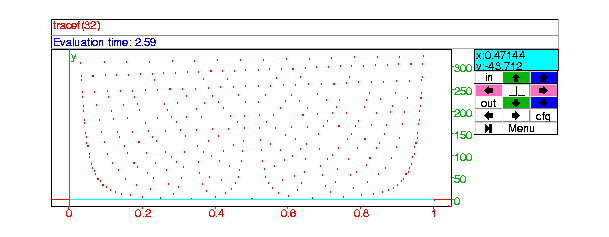
\includegraphics[width=\textwidth]{tracer}}\end{center}
On tape :
\begin{center}{\tt tracef(40)}\end{center}
On obtient :
\begin{center}\framebox{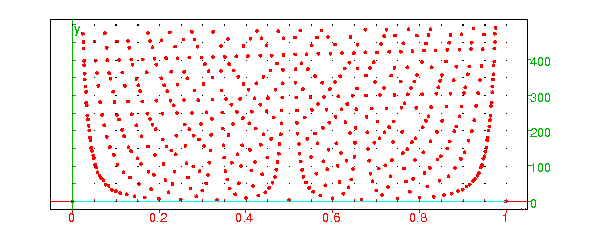
\includegraphics[width=\textwidth]{trace40}}\end{center}{\bf Remarque}
Si on tape 
\begin{verbatim}
tracer(n):={
  local L,a,b;
  L:=point(0),point(1);
  for (b:=2;b<n;b:=b+1){
    for (a:=1;a<b;a:=a+1){
      if (gcd(a,b)==1){L:=L,point(evalf(a/b)+i*f(a/b));}
    }
  }
  return affichage(L,rouge+point_point+
  epaisseur_point_2);
}:;
\end{verbatim}
Le temps de r\'eponse est beaucoup plus long car le programme calcule \`a 
chaque \`etape {\tt f(a/b)} sans tenir compte des valeurs de {\tt f} 
calcul\'ees auparavant. Le temps mis pour faire 
{\tt tracer(100)} est de 160.02s  alors que celui de
{\tt tracef(100)} est de 3.52s.\\
On peut encore diminuer le temps de calcul en stockant par r\'ef\'erence 
(avec {\tt =<} au lieu de {\tt :=}) les 
points dans la liste {\tt L}. Pour cela il faut connaitre la longueur  {\tt s}
de la liste  {\tt L} qui est {\tt f((n-1)/n)}.\\
On tape :
\begin{verbatim}
tracerf(n):={
  local L,a,b,valf,s,j;
  s:=f((n-1)/n);
  L:=makelist(0,1,s);
  L[0]=<point(0);
  L[1]=<point(1);
  valf:=1;
  j:=2;
  for (b:=2;b<=n;b:=b+1){
    for (a:=1;a<b;a:=a+1){
      if (gcd(a,b)==1) {
        valf:=valf+1;
        L[j]=<point(evalf(a/b)+i*valf);
        j:=j+1;
      }
    }
  }
  return affichage(L,rouge+point_point+
  epaisseur_point_2);
}:;
\end{verbatim}
On tape :
\begin{center}{\tt tracerf(100)}\end{center}
On obtient en 0.89s :
\begin{center}\framebox{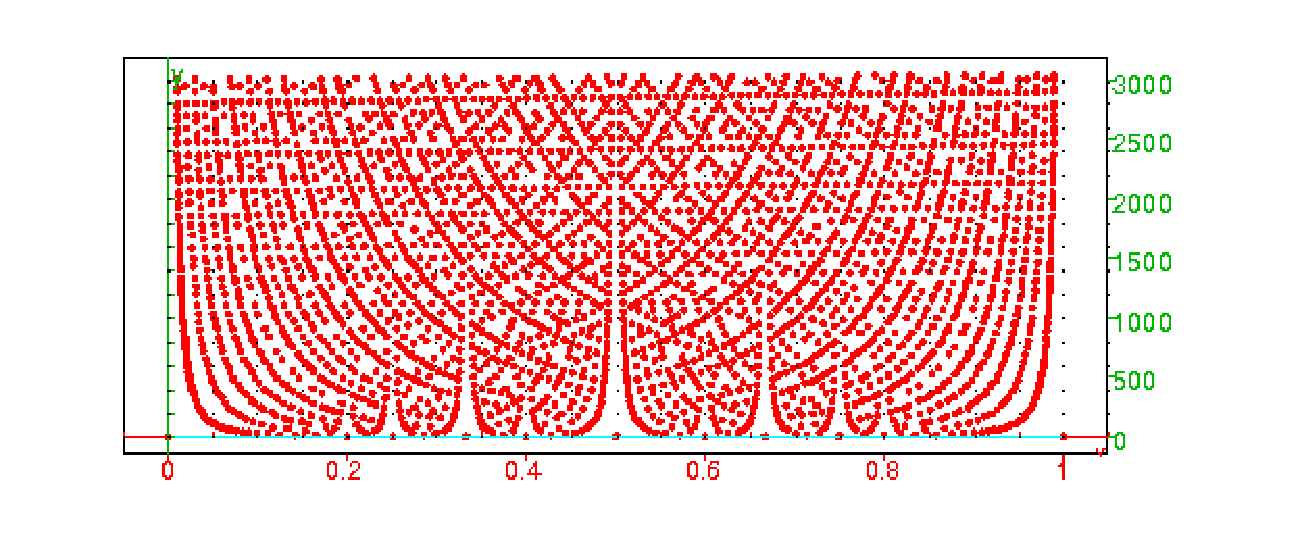
\includegraphics[width=\textwidth]{trace100}}\end{center}
\item On met un peu de couleur ....\\
  On tape :
\begin{verbatim}
tracerfc(n):={
  local L,a,b,valf,s,j;
  s:=f((n-1)/n);
  L:=makelist(0,1,s);
  L[0]=<point(0);
  L[1]=<point(1);L:=point(0),point(1);
  valf:=1;j:=2
  for (b:=2;b<=n;b:=b+1){
    for (a:=1;a<b;a:=a+1){
      if (gcd(a,b)==1) {
        valf:=valf+1;
        L[j]=<point(evalf(a/b)+i*valf,affichage=
        irem(a,7)+point_point+epaisseur_point_2);
        j:=j+1;
      }
    }
  }
  return L;
}:;
\end{verbatim}
On tape :
\begin{center}{\tt tracerfc(100)}\end{center}
On obtient en 0.84s :
\begin{center}\framebox{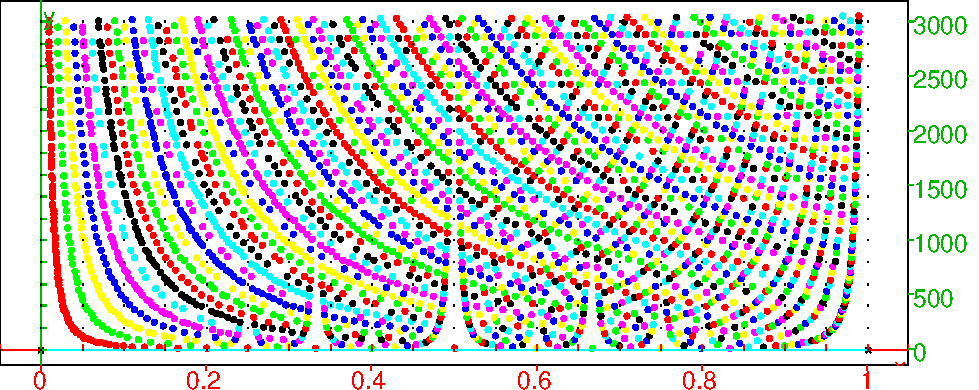
\includegraphics[width=\textwidth]{tracec100}}\end{center}
On remarque que les points $(1/(n+1),f(1/(n+1)))$ et les points 
$((n-1)/n,f((n-1)/n))$ semblent \^etre sur des courbes sym\'etriques par rapport
\`a $x=1/2$, cela s'explique puisque $f((n-1)/n)+1=f(1/(n+1))$.
\end{enumerate}
\subsection{Prolongement du {\bf TP} sur l'indicatrice d'Euler}
{\bf Approximation d'un nuage de points} \\
La fonction $f$ est la bijection entre $\Q \cap [0,1]$ et $\N$ qui a \`et\'e 
d\'efinie dans le {\bf TP} pr\'ec\'edent.
\begin{enumerate}
\item \`A l'aide du tableur tracer le nuage de points de coordonn\`ees :
$\displaystyle \frac{1}{n},f(\frac{1}{n})$ o\`u $f$ est la fonction d\'efinie 
pr\'ec\'edement. On rappelle que l'on a :\\
$$f(\frac{1}{n})=1+\sum_{k=0}^{n-1}\Phi(k) \mbox{ pour } n\in \N^*$$
o\`u $\Phi$ est la fonction d'Euler.
\item On se demande si ces points sont sur une courbe identifiable. Dans le 
livre d'Hardy and Wright d'introduction \`a la th\'eorie des nombres, il est 
dit que $\displaystyle \sum_{k=0}^{n-1}\Phi(k)\simeq \frac{3n^2}{\pi^2}$ pour 
$n$ grand. V\'erifier ce r\'esultat en utilisant une r\'egression convenable.
\item Faites une simulation pour v\'erifier que si on tire au hasard deux 
entiers et qu'avec ces 2 entiers on forme une fraction  de ]0;1], la 
probabilit\'e d'obtenir une fraction irr\'eductible est \'egale \`a $6/\pi^2$.
\item Faites une simulation pour v\'erifier que si on tire au hasard deux 
entiers la probabilit\'e d'obtenir deux entiers premiers entre eux est \'egale 
\`a $6/\pi^2$.
\end{enumerate}
\subsection{Corrig\'e du prolongement du {\bf TP} sur l'indicatrice d'Euler}
\begin{enumerate}
\item On ouvre le tableur avec par exemple 100 lignes.
                                  \begin{itemize}
                                  \item dans la colonne {\tt A}, on met la suite des nombres
                                    entiers $1,2....$,
                                  \item dans la colonne {\tt B}, on met l'inverse de ces nombres.
                                    Pour cela on met dans {\tt B0} : {\tt 1} et dans {\tt B1} : {\tt =\$B\$0/A1} ou 
plus simplement {\tt =1/A1}.\\
Puis on copie cette formule vers le bas.
\item dans la colonne {\tt C}, on met dans {\tt C0} :  {\tt 1}, 
dans {\tt C1} : {\tt =euler(A0)+C0} et dans {\tt C2} : {\tt =euler(A1)+C1}. 
Puis on copie cette formule vers le bas. 
\end{itemize}  
On s\'electionne les 2 colonnes {\tt B} et {\tt C}, puis dans le menu 
{\tt Maths->2-d stats} on choisit {\tt nuage de points} la plage de cellule est alors : {\tt B0:C99} et la cellule cible {\tt D0} si on a coch\'e 
{\tt Graphe} et d\'ecoch\'e {\tt Paysage} dans la configuration du tableur.\\ 
On obtient :
\begin{center}\framebox{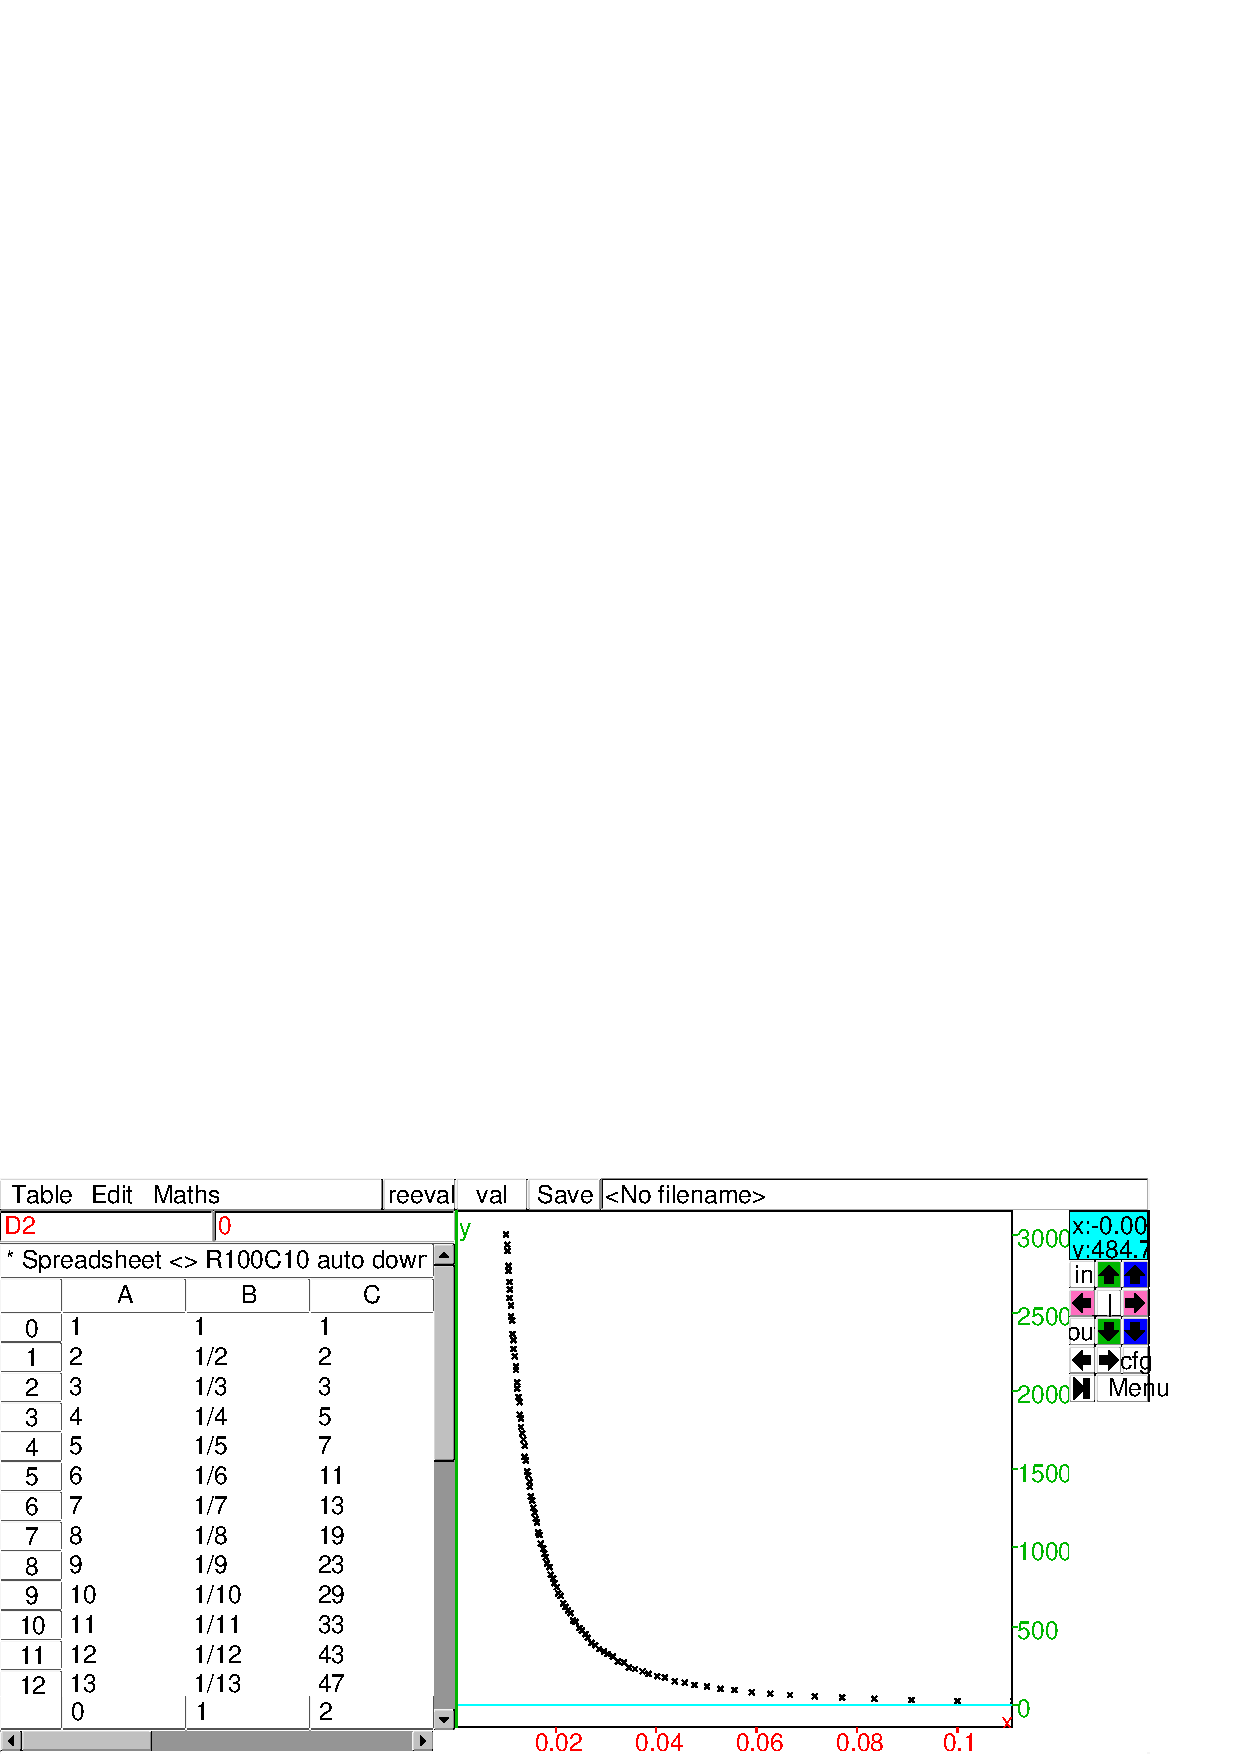
\includegraphics[width=\textwidth]{tracer1n}}\end{center}
\item On modifie {\tt B0} en {\tt 1.0} pour avoir des nombres approch\'es dans 
la colonne {\tt B}. Puis on s\'electionne les 2 colonnes {\tt B} et {\tt C}, 
puis dans le menu {\tt Maths->Regressions} on choisit {\tt Puissance} la plage 
de cellule est alors : {\tt B40:C99} et la cellule cible {\tt D1} (on a coch\'e 
{\tt Graphe} et d\'ecoch\'e {\tt Paysage} dans la configuration du tableur), 
puis on modifie {\tt D1} en :\\
{\tt =power\_regression\_plot(matrix(50,2,(B50):(C99)),color=rouge)} et on 
obtient en rouge :
\begin{center}\framebox{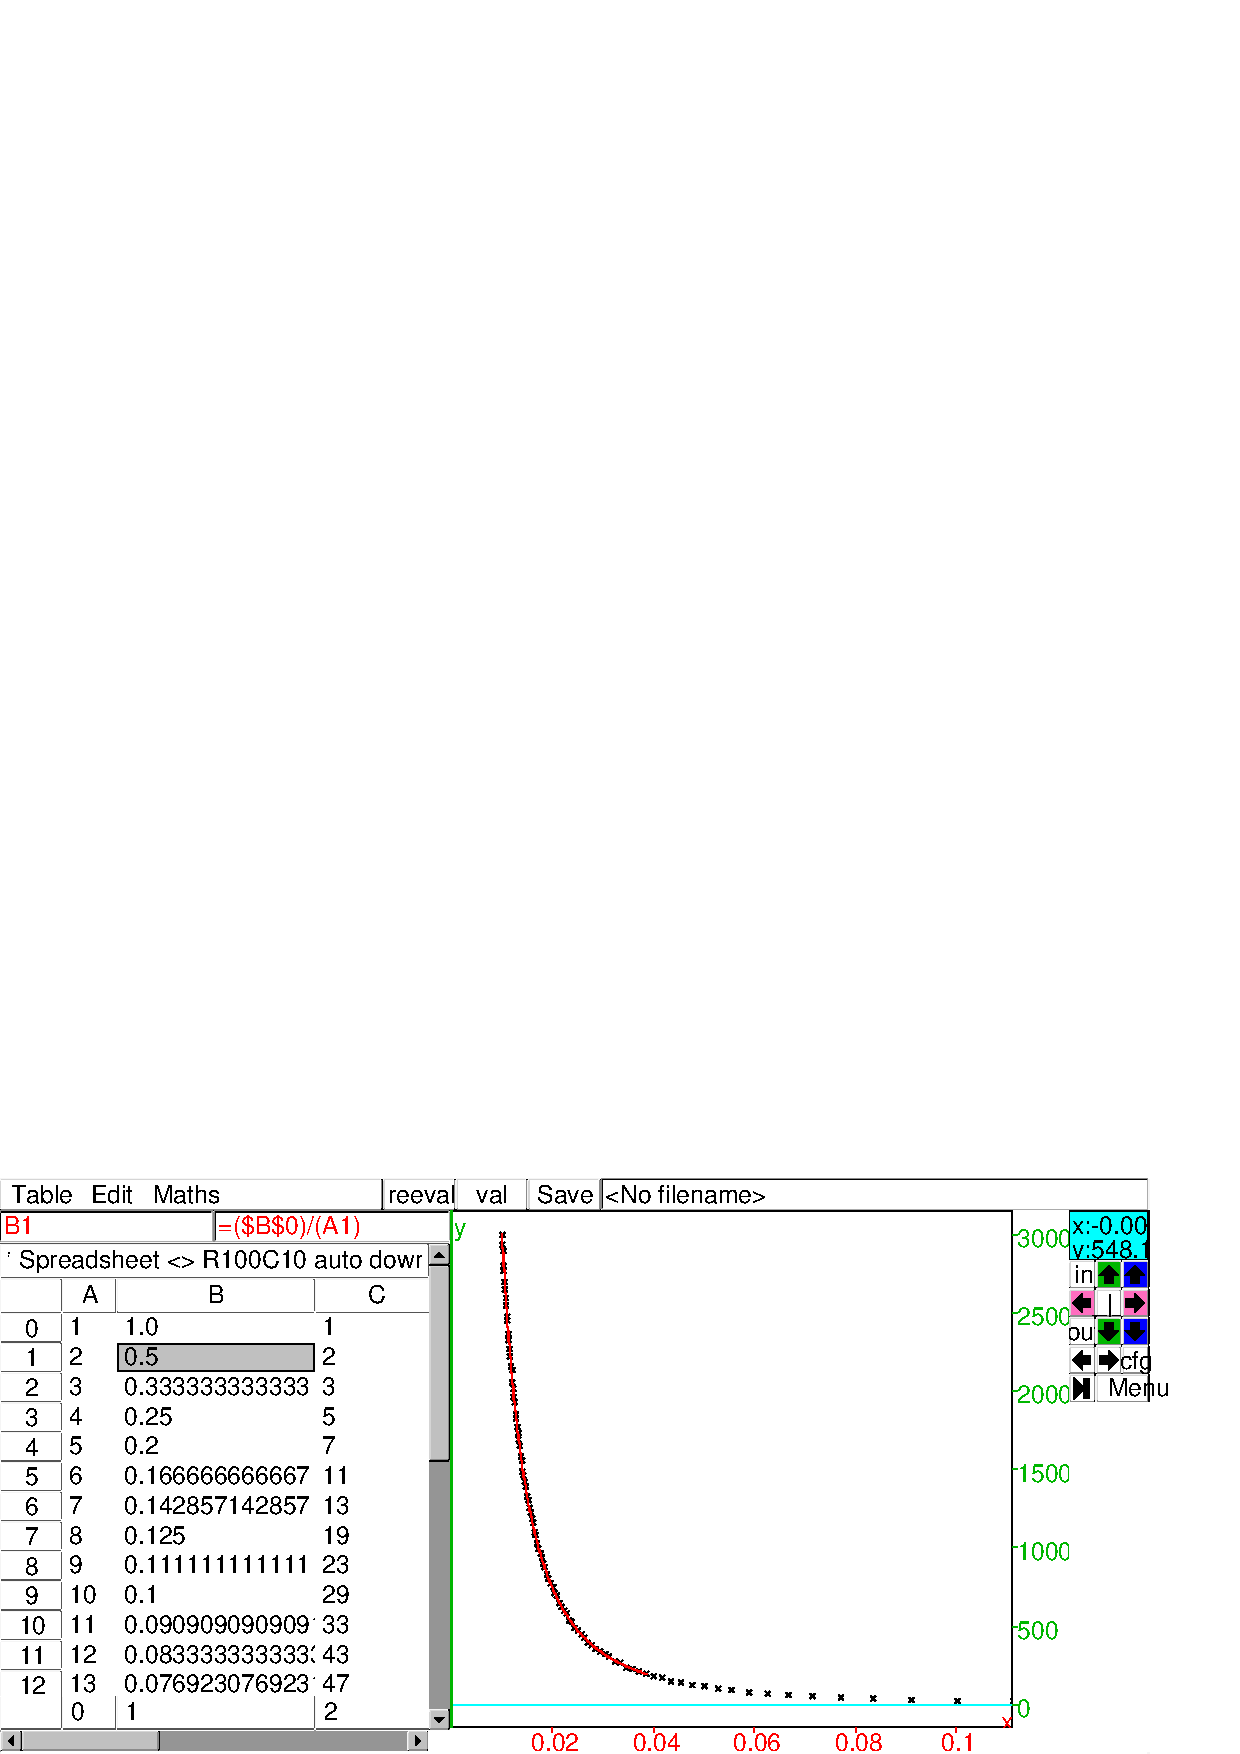
\includegraphics[width=\textwidth]{tracer1r}}\end{center}
\item on met dans {\tt D2} {\tt =(M:=matrix(60,2,(B40):(C99)))}.\\
Puis on tape : 
{\tt =power\_regression(M)}\\
On obtient :
{\tt -2.01348683765,0.283029041082}\\
                              
Ce qui veut dire que $y=0.283029041082*x^-2.01348683765$ approche la courbe 
$y=f(x)$, c'est \`a dire que $f(1/n)\simeq 0.283029041082*n^{2.01348683765}$.\\
On tape : {\tt evalf(3/pi\verb|^|2)}\\
On obtient : {\tt 0.303963550927}
\item On \'ecrit tout d'abord le programme :
\begin{verbatim}
fractirred0(n,p):={
  local a,b,j,k;
  randseed;
  k:=0;
  pour j de 1 jusque p faire
  a:=rand(n)+1;
  b:=rand(n)+1;
  si gcd(a,b)==1 alors k:=k+1;fsi;
  fpour;
  retourne evalf(k/p),evalf(6/pi^2);
}:;
\end{verbatim}
On tape :\\
{\tt fractirred0(100000,1000000)}\\
On obtient :\\
{\tt 0.607658,0.607927101854}\\
On tape :\\
{\tt fractirred0(1000000,1000000)}\\
On obtient :\\
{\tt 0.607544,0.607927101854}\\
On tape :\\
{\tt fractirred0(2\verb|^|31,10\verb|^|6)}\\
On obtient :\\
{\tt 0.607876,0.607927101854}\\
Mais ce programme n'est pas correct car pour le couple $(a,b)$ peut prendre 
$n^2$ valeurs alors que les fractions $a/b \in ]0;1]$ avec $b\leq n$ sont au 
    nombre de $n(n+1)/2$.\\
\begin{verbatim}
fractirred1(n,p):={
  local a,b,j,k;
  randseed;
  k:=0;
  pour j de 1 jusque p faire
  b:=rand(n)+1;
  repeter a:=rand(n)+1;jusqua a<=b;
  si gcd(a,b)==1 alors k:=k+1;fsi;
  fpour;
  retourne evalf(k/p),evalf(6/pi^2);
}:;
\end{verbatim}
On tape :\\
{\tt fractirred1(10000,10000)}\\
On obtient :\\
{\tt 0.6065,0.607927101854}\\
Mais l'ex\'ecution rique d'\^etre longue car si on a tirer pour $b$ 0 ou 1, 
trouver un $a$ plus petit risque de prendre du temps !!!! 
Pour faire un programme plus "rigoureux", on va num\'eroter les fractions sans 
enlever les fractions r\'eductibles (par ex le rang de 2/2 est 3 et celui de 2/6
est 17) puis tirer au hasard un nombre dans 
$(1,2,...n(n+1)/2)$ et chercher la fraction ayant ce rang comme valeur.\\
On tape :\\
\begin{verbatim}
randfract(n):= {
  local r,a,p,q;
  a:=n*(n+1)/2;
  r:=rand(a)+1;
  q:=floor((-1+sqrt(8*r+1))/2);
  p:=r-q*(q+1)/2;
  retourne p,q;
}:;
fractirred(n,p):={
  local a,b,j,k;
  randseed;
  k:=0;
  pour j de 1 jusque p faire
  a,b:=randfract(n);
  si gcd(a,b)==1 alors k:=k+1;fsi;
  fpour;
  retourne evalf(k/p),evalf(6/pi^2);
}:;
\end{verbatim}
On tape :\\
{\tt fractirred(1000,10000)}\\
On obtient :\\
{\tt 0.6059,0.607927101854}\\  
On tape :\\
{\tt fractirred(60000,100000)}\\
On obtient :\\
{\tt 0.60509,0.607927101854}\\  
{\bf Remarque}
Calculons la probabilit\'e d'avoir une fraction irr\'eductible parmi toutes 
les fractions de ]0;1] qui ont un d\'enominateur $d\leq n$.\\
Le nombre total de ces fractions est $n(n+1)/2$, en effet il y a :\\
1 fraction de d\'enominateur 1,\\ 
2 fractions de d\'enominateur 2,..\\
$n$ fractions de d\'enominateur $n$\\ 
donc en tout $n(n+1)/2$ fractions de ]0;1] de d\'enominateur $d\leq n$,\\
Le nombre des fractions irr\'eductibles parmi ces fractions est 
$\sum_{k=1}^n${\tt euler}$(k)$, en effet il y a :\\
{\tt euler(1)=1} fraction irr\'eductible de d\'enominateur 1,\\
{\tt euler(2)=1} fraction irr\'eductible de d\'enominateur 2,..\\
{\tt euler(n)} fractions irr\'eductibles de d\'enominateur $n$ \\
donc en tout {\tt euler(1)+euler(2)+..+euler(n)} fractions irr\'eductibles de 
d\'enominateur $d\leq n$.\\
On tape :\\
{\tt 2*sum(euler(k),k=1..1000)/(1000\verb|^|2+1000.)}\\
On obtient :
{\tt 0.607776223776}\\
On tape :\\
{\tt 2*sum(euler(k),k=1..10000)/(10000\verb|^|2+10000.)}\\
On obtient :
{\tt 0.607888931107}\\
Si on suppose que $n$ est grand et que l'on a montr\'e que 
$\sum_{k=0}^{n-1}\Phi(k)\simeq \frac{3n^2}{\pi^2}$, la probabilit\'e d'avoir une
fraction irr\'eductible parmi toutes 
les fractions de [0;1] qui ont un d\'enominateur $d\leq n$ est :\\
$\sum_{k=1}^n euler(k)\simeq \frac{2*3*(n+1)^2}{\pi^2*n*(n+1)}=\frac{6*(n+1)}{n\pi^2}$.
Cette probabilit\'e tend donc vers $\frac{6}{\pi^2}$ quand $n$ tend vers 
l'infini.\\
{\bf Id\'ee pour montrer que si on tire au hasard 2 nombres entiers, la 
probabilit\'e d'obtenir deux entiers premiers entre eux est \'egale \`a 
$6/\pi^2$}\\
Cette propri\'et\'e r\'esulte du fait que $\frac{\pi^2}{6}$ est la somme de la 
s\'erie de terme g\'en\'eral $u_n=\frac{1}{n^2}$ i.e.
$\sum_{n=1}^{+\infty}\frac{1}{n^2}=\frac{\pi^2}{6}$.\\
 En effet, soit $p$ un nombre premier.\\
La probabilit\'e pour qu'un entier pris au hasard soit divisible par $p$ (i.e. 
multiple de $p$) est \'egale \`a $\frac{1}{p}$ (la probabilit\'e
pour qu'un entier pris au hasard soit divisible pair est \'egale \`a 
$\frac{1}{2}$, la probabilit\'e pour qu'un entier pris au hasard soit 
divisible par $3$ est \'egale \`a $\frac{1}{3}$...)\\
La probabilit\'e pour que deux entiers pris au hasard soient tous les deux 
divisibles par $p$ est \'egale \`a $\frac{1}{p^2}$. \\
Donc la probabilit\'e pour que le pgcd de deux entiers pris au 
hasard ne soit pas divisible par $p$ est \'egale \`a $1-\frac{1}{p^2}$.\\
Donc, si $NP$ est l'ensemble des nombres premiers, la probabilit\'e pour que le 
pgcd de deux entiers pris au hasard soit \'egal \`a 1 (i.e. divisible par aucun 
nombre premier) est \'egale \`a $\Pi_{p\in NP}(1-\frac{1}{p^2})$.\\
Il faut maintenant \'ecrire autrement $\Pi_{p\in NP}(1-\frac{1}{p^2})$ ou 
plut\^ot son inverse $\Pi_{p\in NP}\frac{1}{1-\frac{1}{p^2}}$.\\
On sait que $\frac{1}{1-t^2}=\sum_{n=0}^{+\infty}t^{2n}$ donc
$\frac{1}{1-\frac{1}{p^2}}=\sum_{n=0}^{+\infty}\frac{1}{p^{2n}}$.\\
Finallement $\Pi_{p\in NP}\frac{1}{1-\frac{1}{p^2}}=\Pi_{p\in NP}\sum_{n=0}^{+\infty}\frac{1}{p^{2n}}$\\
Comme les nombres entiers sont le produit de nombres premiers \a une certaine 
puissance, on a :\\
$\Pi_{p\in NP}\frac{1}{1-\frac{1}{p^2}}=\Pi_{p\in NP}\sum_{n=0}^{+\infty}\frac{1}{p^{2n}} =\sum_{k=0}^{+\infty}\frac{1}{k^{2}}=\frac{\pi^2}{6}$.\\
Ainsi $\Pi_{p\in NP}(1-\frac{1}{p^2})=\frac{6}{\pi^2}$
\end{enumerate}
\section{Le probl\`eme de Joseph Bertrand (1822-1900)}
Soit un cercle de rayon $R$. On appelle corde type les cordes de longueur 
$a=R\sqrt 3$. La longueur des cordes types est \'egale \`a la longueur des 
c\^ot\'es des triangles \'equilat\'eraux inscrits dans ce cercle. Le probl\`eme
de Joseph Bertrand est :\\
quelle est la probabilit\'e pour qu'une corde prise au hasard soit plus grande 
qu'une corde type ?\\
\'Ecrire un programme qui simule le choix d'une corde prise au hasard dans un 
cercle de rayon $1$ lorsque :
\begin{enumerate}
\item On prend 2 points au hasard sur le cercle pour d\'eterminer une corde,
\item  On prend 1 point au hasard sur le cercle et une direction au hasard ce 
qui d\'eterminera une corde.
\item On prend 1 point d\'efini au hasard par ses coordonn\'ees cart\'esiennes 
dans le cercle. Ce point d\'eterminera le milieu de 
la corde (et donc la corde),
\item On compare les cordes qui ont la m\^eme direction : pour cela, pour
chaque direction $d$, on prend un r\'eel $r$ au hasard entre 
$-R$ et $R$ et cela d\'efini 1 point sur le rayon orthogonal \`a $d$. Ce point 
d\'eterminera le milieu de la corde (et donc la corde). 
 \end{enumerate}
Puis expliquez les r\'esultats obtenus.\\

{\bf Les programmes avec Xcas}\\
Une corde type $AB$ d'un cercle de rayon 1 a pour longueur $\sqrt 3$ et son 
angle au centre vaut $2\pi/3$ i.e si $a$ est l'argument de l'affixe de $A$ et 
$b$ est l'argument de l'affixe de $B$.
\begin{enumerate}
\item On prend 2 points $A$ et $B$ au hasard sur le cercle pour d\'eterminer 
une corde. Ces 2 points seront d\'etermin\'es par leur arguments $a$ et $b$ 
choisis au hasard entre $-\pi$0 et $\pi$. Ces deux points d\'efinissent une 
corde de longueur sup\'erieure  \`a $\sqrt 3$ si \\
$l=AB^2=\mbox{abs}(\exp(i*a)-\exp(i*b))^2=2-2\cos(a-b)> 3$ ou si \\
$2\pi/3<|a-b|<4\pi/3$.
Cela donne les 2 programmes {\tt simulber10} et {\tt simulber11}.
Le programme {\tt simulber10} \'etant plus rapide puisqu'il n\'ecessite qu'un 
seul test.\\
On tape :
\begin{verbatim}
simulber10(n):={
  local j,a,b,l,s;
  s:=0;
  pour j de 1 jusque n faire
  a:=rand(-pi,pi);
  b:=rand(-pi,pi);
  l:=2-2*cos(a-b);
  si l>3 alors s:=s+1; fsi;
  fpour;
  retourne s,n,evalf(s/n);
}:;
simulber11(n):={
  local j,a,b,c,s;
  s:=0;
  pour j de 1 jusque n faire
  a:=rand(-pi,pi);
  b:=rand(-pi,pi);
  c:=abs(a-b);
  si c>2*pi/3 et c<4*pi/3 alors s:=s+1; fsi;
  fpour;
  retourne s,n,evalf(s/n);
}:;
\end{verbatim}
On tape :
{\tt simulber10(100000) }\\
On obtient : {\tt 33315,100000,0.33315}\\
On tape :
{\tt simulber11(100000) }\\
On obtient : {\tt 33410,100000,0.3341}\\
Dans ces 2 programmes ce qui compte c'est la valeur de $|b-a|$ qui est un 
nombre entre 0 et $2\pi$. Il y a donc une chance sur trois pour que ce nombre 
soit compris entre $2\pi/3$ et $4\pi/3$.
\item On prend 1 point $A$ au hasard sur le cercle et une direction $d$ au 
  hasard pour d\'eterminer une corde. Le point $A$ sera d\'etermin\'e par son 
 argument $a$ choisi au hasard entre $-\pi$ et $\pi$ et la direction $D$ par son
angle $d$ avec l'axe des $x$ que l'on choisit au hasard entre 0 et $\pi$. 
 Ce point et la direction d\'efinissent une corde $AB$ de longueur sup\'erieure 
  \`a $\sqrt 3$ si $(a+b)/2=\pi/2-d$ (c'est \`a dire $b=\pi+2d-a$).\\
  On tape :
\begin{verbatim}
simulber2(n):={
  local j,a,b,d,l,s;
  s:=0;
  pour j de 1 jusque n faire
  a:=rand(-pi,pi);
  d:=rand(0,pi);
  b:=pi+2*d-a;
  l:=2-2*cos(a-b);
  si l>3 alors s:=s+1; fsi
  fpour
  retourne s,n,evalf(s/n);
}:;
\end{verbatim}
On tape :
{\tt simulber2(100000)}\\
On obtient : {\tt 33264,100000,0.33264}\\
On a le m\^eme r\'esultat qu'en 1, puisque c'est pratiquement le m\^eme 
programme.
\item On d\'efinit au hasard dans le cercle le milieu de la corde par ses 
  coordonn\'ees cart\'esiennes.
\begin{verbatim}
simulber3(n):={
  local j,a,b,c,l,s;
  s:=0;
  pour j de 1 jusque n faire
  repeter
  a:=rand(-1,1);
  b:=rand(-1,1);
  jusqua a^2+b^2<1;
  l:=4*(1-a^2-b^2);
  si l>3 alors s:=s+1; fsi;
  fpour;
  retourne s,n,evalf(s/n);
}:;
\end{verbatim}
On peut remplacer 
{\tt l:=4*(1-a\verb|^|2-b\verb|^|2);si l>3 alors s:=s+1; fsi;} par \\
{\tt l:=a\verb|^|2+b\verb|^|2;si l<1/4 alors s:=s+1; fsi;}\\
On tape :
{\tt simulber3(100000)}\\
On obtient : {\tt 25039,100000,0.25039}\\
Le cercle de rayon 1/2 a comme surface $\pi/4$ et celui de rayon 1 a comme 
surface $\pi$. La probabilit\'e de se trouver dans le cercle de rayon 1/2 est 
donc de 1/4.\\
{\bf Attention} Si on \'ecrit :
\begin{verbatim}
simulber30(n):={
  local j,a,b,c,l,s;
  s:=0;
  pour j de 1 jusque n faire
  a:=alea(-1,1);
  c:=sqrt(1-a^2);
  b:=alea(-c,c);
  l:=4*(1-a^2-b^2);
  si l>3 alors s:=s+1; fsi;
  fpour;
  retourne s,n,evalf(s/n);
}:;
\end{verbatim}
le programme n'est pas correct car dans ce programme $a$ et $b$ ne sont pas 
ind\'ependants (voir la remarque du \ref{sec:buffon}).\\
On tape :
{\tt simulber30(100000)}\\
On obtient : {\tt 20311,100000,0.20311}
On fait le calcul de la probabilit\'e avec ce programme.\\
La probabilit\'e d'avoir : $a<x<a+da$ et $b<y<db$ est :
$da*db/aire(S)$ avec $S=\{(x,y) a<x<a+da,0<y<\sqrt{1-a^2}\}$.\\
On obtient si $\cos(t_1)=a$ et $\cos(t_2)=a+da$: avec $dt=-da/\sqrt{1-a^2}$\\
$aire(S)=2(t_1-t_2)+\sin(2t_2)-\sin(2t_1)=2dt(\cos(2t_1)-1)=4da\sqrt{1-a^2}$
donc $db=1/(4\sqrt{1-a^2})$\\
On a :\\
$\int_0^1\frac{\sqrt(1-x^2)}{\sqrt(1-x^2)dx}=1$ donc la probbilit\'e d'\^etre
dans le cercle de rayon 1/2 est :\\
$\int_0^{\frac{1}{2}}\frac{\sqrt(\frac{1}{4}-x^2)}{\sqrt(1-x^2)dx}$
0n tape 
{\tt romberg(sqrt((1/4-x\verb|^|2))/sqrt((1-x\verb|^|2)),x=0..1/2)} \\
On obtient (avec 7 digits) : {\tt 0.20315486}

\item On d\'efinit au hasard un nombre r\'eel $r$ entre $-R$ et $R$. la longueur
  $l$ de la corde de direction $d$ et dont  la distance au centre est 
  $r$ est : $l=2\sqrt{1-r^2}$ et $l$ ne d\'epend pas de la direction. Donc pour 
  une direction donn\'ee la probabilit\'e cherch\'ee ne d\'epend pas de la 
  direction.\\
  On tape (dans le programme $R=1$ et$l$ est le carr\'e de la longueur de la corde) :
\begin{verbatim}
simulber4(n):={
  local j,r,l,s;
  s:=0;
  pour j de 1 jusque n faire
  r:=rand(-1,1);
  l:=4*(1-r^2);
  si l>3 alors s:=s+1; fsi
  fpour
  retourne s,n,evalf(s/n);
}:;
\end{verbatim}
On tape :
{\tt simulber4(100000)}\\
On obtient : {\tt 49993,100000,0.49993}\\
En effet, on a  $l={AB}^2=4*(1-r^2)$ et donc les conditions $l>3$ et $0<r<1/2$ 
sont \'equivalentes.\\ 
Donc pour une direction donn\'ee la probabilit\'e cherch\'ee est 1/2 et elle
ne d\'epend pas de la direction.œn en conclut que par rapport \`a la corde type,
il y a autant de cordes longues que de cordes courtes.
{\bf Remarque}\\
Lorsqu'on d\'efinit au hasard dans le cercle le milieu $M$ de la corde par ses 
coordonn\'ees polaires $r,t$ (i.e. l'affixe de $M$ est $m=r\exp(it)$).
Pour cela on choisit un r\'eel $r$ au hasard entre 
$-R$ et $R$ et un angle $t$ r\'eel au hasard  entre  0 et $\pi$ ce qui 
d\'eterminera le point $r \exp(it)$.\\
On tape :
\begin{verbatim}
simulber40(n):={
  local j,r,t,m,l,s;
  s:=0;
  pour j de 1 jusque n faire
  r:=rand(-1,1);
  t:=rand(0,pi);
  m:=r*exp(i*t);
  l:=4*(1-r^2);
  si l>3 alors s:=s+1; fsi
  fpour
  retourne s,n,evalf(s/n);
}:;
\end{verbatim}
On tape :
{\tt simulber40(100000)}\\
On obtient : {\tt 50068,100000,0.50068}\\
En effet, on voit que la valeur de $t$ ne sert pas et que $l={AB}^2$ ne 
d\'epend que de $r$. Les conditions $l>3$ et $0<r<1/2$ sont \'equivalentes. 
Donc la probabilit\'e cherch\'ee est encre 1/2.\\
{\bf Question} Pourquoi selon que l'on choisit le milieu de la corde avec ses 
coordonn\'ees cart\'esiennes ou avec ses coordonn\'ees polaire la probabilit\'e
passe de 1/4 \`a 1/2 ?\\
Il faut comprendre que :
\begin{verbatim}
r:=rand(-1,1);
t:=rand(0,pi);
M:=point(r*exp(i*t));
\end{verbatim}
ne d\'efinit pas des points \'equir\'epartis dans le cercle de centre $0$ et de 
rayon 1.\\
Il y a plus de points proche du centre que sur la p\'eriph\'erie (voir la remarque du \ref{sec:buffon}).
\end{enumerate}

\section{Un exercice sur les congruences et les restes chinois}
\subsection{L'\'enonc\'e}
Trouver un nombre entier $n$ v\'erifiant $4<n<N$ v\'erifiant :\\
$n$ est divisible par 2\\
$n-1$ est divisible par 3\\
$n-2$ est divisible par 5\\ 
$n-3$ est divisible par 7\\
$n-4$ est divisible par 11

\subsection{Solution avec {\tt Xcas} et les restes chinois}
On utilise la commande {\tt ichinrem}.\\
On tape :\\
{\tt ichinrem([0\%2,1\%3,2\%5,3\%7,4\%11]))}\\
On obtient :
{\tt -788 \% 2310}\\
On veut que $0<n<N$ donc  :\\
$n=(2310-788)+2310*k=1522+2310*k$ avec $k\leq \mbox{iquo}((N-1522),2310)$
donc si $N=10000$ on tape :\\
{\tt iquo((10000-1522),2310)}\\
On obtient :\\
{\tt 3}\\
On tape :\\
{\tt (1522+2310*k)\$(k=0..3)}\\
On obtient :\\
{\tt 1522,3832,6142,8452}

\subsection{Solution avec {\tt Xcas} et l'identit\'e de B\'ezout}
On utilise la commande {\tt iabcuv} qui \'etant donn\'e trois entiers
{\tt a,b,c} renvoie une liste de deux entiers 
relatifs {\tt [u,v]} v\'erifiant {\tt a*u+b*v=c}.\\
{\bf Remarque} 
\begin{itemize}
\item Si deux entiers 
  relatifs $u,v$ v\'erifie $au+bv=c$ alors on a aussi :\\
  $a(u+kb)+b(v-ka)=c$ pour tout $k \in \Z$.
\item {\tt iabcuv} est une g\'en\'eralisation de l'identit\'e de B\'ezout
  (commande {\tt iegcd}). On a en effet :
  {\tt iegcd(a,b)} renvoie une liste de trois entiers {\tt [u,v,d]} 
  v\'erifiant {\tt a*u+b*v=d=gcd(a,b)} (o\`u {\tt gcd(a,b)} est
  le  pgcd de {\tt a} et {\tt b}).\\
  Donc pour que {\tt iabcuv} ait une solution il faut et il 
  suffit que {\tt c} soit un multiple du pgcd de {\tt a} et {\tt b}.
  Donc {\tt iabcuv} a toujours une solution si {\tt a} et {\tt b} sont premiers 
  entre eux.
\end{itemize}
On cherche $n$ v\'erifiant :\\
$n$ est un multiple de 2 et aussi un  multiple de 3 plus 1. \\
Donc on a : $n=2p=3q+1$ avec $p\in \Z$ et $q\in \Z$.\\
c'est \`a dire $2p-3q=1$.\\
On tape : {\tt iabcuv(2,3,1)}\\
On obtient : {\tt [-1,1]}\\
Donc $n=2*(-1+3k)=-2\ \%\ 6$.\\
De plus $n$ est un multiple de 5 plus 2.\\
Donc on a : $n=5r+2=-2+6k$ avec $r\in \Z$ et $k\in \Z$.\\
c'est \`a dire $6k-5r=4$.\\
On tape : {\tt iabcuv(6,5,4)}\\
On obtient : {\tt [-1,2]}\\
Donc $n=6*(-1+5k)-2=-8\ \%\  30$.\\
De plus $n$ est un multiple de 7 plus 3.\\
Donc on a : $n=7j+3=-8+30k$ avec $j\in \Z$ et $k\in \Z$.\\
c'est \`a dire $30k-7j=11$.\\
On tape : {\tt iabcuv(30,7,11)}\\
On obtient : {\tt [2,-7]}\\
Donc $n=30*(2+7k)-8=52\ \%\ 210$.\\
De plus $n$ est un multiple de 11 plus 4.\\
Donc on a : $n=11m+4=52+210k$ avec $m\in \Z$ et $k\in \Z$.\\
c'est \`a dire $11m-210k=48$.\\
On tape : {\tt iabcuv(11,210,64)}\\
On obtient : {\tt [-72,4]}\\
Donc $n=11*(-72+210k)+4=-788\ \%\ 2310$.\\
On tape : {\tt (-788+k*2310)\$ (k=1..4)}\\
On obtient : {\tt 1522,3832,6142,8452}
\chapter{Matrices en terminale scientifique}
\section{Les matrices de rotation}
\'Etant donn\'e $t\in \R$ on consid\`ere :\\
$A(t)=\left(
\begin{array}{cc}
  \cos(t)&-\sin(t)\\
  \sin(t)&\cos(t)
\end{array}
\right)$\\
Calculer $A(t)^n$ pour $n\in \N$.\\
Calculer $A(t)^2-2\cos(t)A(t)+I$ o\`u $I$ est la matrice identit\'e d'odre 2.\\
En d\'eduire que $A(t)$ est inversible et que $A(t)^{-1}=A(-t)$.\\
Calculer $A(t)^n$ pour $n\in \Z$.\\
Montrer que dans un rep\`ere orthonorm\'e $(O;\overrightarrow i,\overrightarrow j)$, la matrice $A(t)$ est la matrice de la rotation de centre $O$ et d'angle $t$.\\
On tape :\\
{\tt A(t):=[[cos(t),-sin(t)],[sin(t),cos(t)]]}\\
{\tt tlin(A(t)*A(t))}\\
On obtient :\\
{\tt [[cos(2*t),-sin(2*t)],[sin(2*t),cos(2*t)]]}\\
On tape :\\
{\tt assume(n,integer)}\\
{\tt An(t):=[[cos(n*t),-sin(n*t)],[sin(n*t),cos(n*t)]]}\\
{\tt tlin(An(t)*A(t))}\\
On obtient :\\
{\tt [[cos(n*t+t),-sin(n*t+t)],[sin(n*t+t),cos(n*t+t)]]}\\
Donc on a montr\'e par r\'ecurrence que :\\
$A(t)^n=A(nt)$.\\
On tape :\\
{\tt tlin(A(t)\verb|^|2-2*cos(t)*A(t)+idn(2))}\\
On obtient :\\
{\tt [[0,0],[0,0]]}\\
On en d\'eduit que :\\
$A(2\cos(t)*I-A)=I$
On tape :\\
{\tt B(t):=normal(2*cos(t)*idn(2)-A(t))}\\
{\tt B(t)}\\
On obtient :\\
{\tt [[cos(t),sin(t)],[-sin(t),cos(t)]]}\\
On tape :\\
{\tt B(t)-A(-t)}\\
On obtient :\\
{\tt [[0,0],[0,0]]}\\
Donc pour tout $n\in \N$, on a $A(t)^{-1}=A(-t)$ et  $A(t)^{-n}=A(-t)^n=A(-nt)$.\\
Donc pour tout $n\in \Z$, on a   $A(t)^{n}=A(nt)$.\\
Dans la rotation $r$ de centre $O$ et d'angle $t$ :\\
le vecteur $\overrightarrow i$ se transforme en le vecteur :
$r(\overrightarrow i)=\cos(t)\overrightarrow i+\sin(t)\overrightarrow j$\\
le vecteur $\overrightarrow j$ se transforme en le vecteur :
$r(\overrightarrow j)=-sin(t)\overrightarrow i+\cos(t)\overrightarrow j$\\
Donc :\\
$r(x\overrightarrow i+y\overrightarrow j)=xr(\overrightarrow i)+yr(\overrightarrow j)=(x\cos(t)-y\sin(t))\overrightarrow i+(x\sin(t)+y\cos(t))\overrightarrow j$\\
c'est \`a dire :\\
$r\left(\begin{array}{c}
  x\\
  y
\end{array}\right)=\left(
\begin{array}{cc}
  \cos(t)&-\sin(t)\\
  \sin(t)&\cos(t)
\end{array}
\right)\left(\begin{array}{c}
  x\\
  y
\end{array}\right)=
A(t)\left(\begin{array}{c}
  x\\
  y
\end{array}\right)$\\
On tape :\\
{\tt coordonnees(rotation(0,t,x+i*y))}\\
On obtient :\\
{\tt [cos(t)*x-sin(t)*y,cos(t)*y+x*sin(t)]}
\section{Les matrices magiques d'odre 3}
\subsection{R\'esultat pr\'eliminaire}
Soit $A$ la matrice :\\
$A=[[a_{00},a_{01},a_{02}],[a_{10},a_{11},a_{12}],[a_{20},a_{21},a_{22}]]$
Montrer que :\\
$B=1/2*(A+\mbox{tran}(A))$ est une matrice sym\'ertrique et\\
$C=1/2*(A-\mbox{tran}(A))$ est une matrice antisym\'ertrique.\\
En d\'eduire que toute matrice se d\'ecompose de fa\c{c}on unique en la somme 
d'une matrice sym\'etrique et d'une matrice antisym\'etrique.\\
On tape :\\
{\tt A:=[[a00,a01,a02],[a10,a11,a12],[a20,a21,a22]]}\\
{\tt B:=1/2*(A+tran(A));C:=1/2*(A-tran(A))}\\
{\tt normal(B-tran(B)),normal(C+tran(C))}\\
On obtient :\\
{\tt [[0,0,0],[0,0,0],[0,0,0]],[[0,0,0],[0,0,0],[0,0,0]]}\\
Si $A=M+N$ avec tran($M$)=$M$ et tran($N$)=$-N$ alors tran($A$)=$M-N$ donc \\
$M=1/2*(A+\mbox{tran}(A))=B$ et $N=1/2*(A-\mbox{tran}(A))=C$ d'o\`u l'unicit\'e.
\subsection{Les matrices magiques d'odre 3}
Une matrice $A=(a_{j,k})$ d'ordre 3 est une matrice magique de somme $s$ lorsque
les 8 sommes :\\
$\sum_{j=0}^2a_{j,k}=s$ pour $k=0,1,2$ (somme de chaque colonne)\\
$\sum_{k=0}^2a_{j,k}=s$ pour $j=0,1,2$ (somme de chaque ligne)\\
$\sum_{j=0}^2a_{j,j}=a_{1,3}+a_{2,2}+a_{3,1}=s$ (somme de chaque diagonale).\\
%On note $M(s)$ les matrices magiques d'ordre 3 de somme $s$
D\'eterminer les matrices magiques d'ordre 3 qui sont antisym\'etriques.\\
D\'eterminer les matrices magiques d'ordre 3 qui sont sym\'etriques de somme 
$s=0$.\\
D\'eterminer une matrice magique d'ordre 3, sym\'etrique, de somme $s$ et la plus simple possible.\\
Montrer que la diff\'erence de 2 matrices sym\'etriques  magiques de somme $s$ est une matrices sym\'etriques  magiques de somme $s=0$.\\
En d\'eduire toutes les matrices magiques d'ordre 3, sym\'etriques de somme $s$.\\
Trouver toutes les matrices magiques d'ordre 3 de somme $s=3$. \\
Trouver toutes les matrices magiques d'ordre 3 de somme $s=9$. \\
Les matrices magiques d'ordre 3 qui sont antisym\'etriques sont de somme $s=0$ 
car la diagonale principale ne contient que des 0.\\
Soit $A$ une matrice antisym\'etrique d'ordre 3 et magique de somme $s=0$.\\
On tape :\\
{\tt A:=[[0,a,b],[-a,0,c],[-b,-c,0]]}\\
{\tt linsolve([a+b=0,-a+c=0,b+c=0],[a,b,c])}\\
On obtient :\\
{\tt [c,-c,c]}\\
Donc les matrices magiques $A$ d'ordre 3 qui sont antisym\'etriques sont  :\\
$A=\left(
\begin{array}{ccc}
  0&c&-c\\
  -c&0&c\\
  c&-c&0
\end{array}
\right)=c\left(
\begin{array}{ccc}
  0&1&-1\\
  -1&0&1\\
  1&-1&0
\end{array}
\right)
$\\
On tape :\\
{\tt A:=c*[[0,1,-1],[-1,0,1],[1,-1,0]]}\\
Soit $S$ une matrice sym\'etrique d'ordre 3 et magique de somme $s=0$.\\
On tape :\\
{\tt S:=[[a,b,c],[b,d,e],[c,e,f]]}\\
{\tt linsolve([a+b+c,a+d+f,b+d+e,c+e+f,2c+d],[a,b,c,d,e,f])}\\
On obtient :\\
{\tt [-f,f,0,0,-f,f]}\\
Donc les matrices magiques $S$ d'ordre 3 qui sont sym\'etriques de somme $s=0$ 
sont  :\\
$S=\left(
\begin{array}{ccc}
  -f&f&0\\
  f&0&-f\\
  0&-f&f
\end{array}
\right)=f\left(
\begin{array}{ccc}
  -1&1&0\\
  1&0&-1\\
  0&-1&1
\end{array}
\right)
$\\
Soit $S_0$ une matrice sym\'etrique d'ordre 3 et magique de somme $s$ la plus simple possible.\\
On tape :\\
{\tt S0:=s/3*[[1,1,1],[1,1,1],[1,1,1]]}\\
Donc les matrices magiques $S$ d'ordre 3 qui sont sym\'etriques de somme $s$ 
sont  $B:=S+S_0$:\\
On tape :\\
{\tt B:=f*[[-1,1,0],[1,0,-1],[0,-1,1]]+\\s/3*[[1,1,1],[1,1,1],[1,1,1]]}\\

Donc les matrices magiques $M$ d'ordre 3 qui sont de somme $s=3$ (resp $s=12$)
sont  $M:=A+S+S_0$ et elles d\'ependent de 2 param\`etres $c$ et $f$.\\
On tape :\\
{\tt M:=c*[[0,1,-1],[-1,0,1],[1,-1,0]]+\\
  f*[[-1,1,0],[1,0,-1],[0,-1,1]]+[[1,1,1],[1,1,1],[1,1,1]]}\\
On obtient :\\
{\tt [[-f+1,c+f+1,-c+1],[-c+f+1,1,c-f+1],[c+1,-c-f+1,f+1]]}
Par exemple $f=1,c=0$, on obtient 
{\tt [[0,2,1],[2,1,0],[1,0,2]]}.\\
On tape :\\
{\tt M:=c*[[0,1,-1],[-1,0,1],[1,-1,0]]+\\
  f*[[-1,1,0],[1,0,-1],[0,-1,1]]+4*[[1,1,1],[1,1,1],[1,1,1]]}\\
On obtient :\\
{\tt [[-f+4,c+f+4,-c+4],[-c+f+4,4,c-f+4],[c+4,-c-f+4,f+4]]}\\
Par exemple $f=1,c=3$, on obtient 
{\tt [[3,8,1],[2,4,6],[7,0,5]]}
\chapter{D\'enombrement}
\section{Nombre d'applications d'un ensemble fini dans un ensemble fini}
Soient deux ensembles $E$ dans $F$ de cardinaux respectifs $p$ et $n$.
Soit $\mathcal{A}(E,F)$ l'ensemble des applications de $E$ dans $F$.
Soit $u(p,n)$ le nombre d'applications de $E$ dans $F$.
On a :
$u(p,1)=p$ car si $E={a}$ et $F={b_1,b_2..b_p}$ les applications de $E$ dans $F$
 sont d\'efinies par :\\
$f_j(a)=b_j)$ avec $1\leq j\leq p$\\
On montre par r\'ecurrence que  $u(p,n)=p*u(p,n-1)$.\\
En effet :\\
si $E={a_1,a_2...a_n}$ et $E_1={a_2...a_n}$, une application de $E$ dans $F$ 
est d\'efinie par une application de $E_1$ dans $F$ et par $f(a_1)=b_j$ pour
$1\leq j\leq p$.\\
Donc $u(p,n)=p^n$

\section{Nombre d'injections d'un ensemble fini dans un ensemble fini : les arrangements}\index{perm}
Soient deux ensembles $E$ dans $F$ de cardinaux respectifs $p$ et $n$ avec 
$n\geq p$.\\
Soit $\mathcal{I}(E,F)$ l'ensemble des injections de $E$ dans $F$.
Soit $v(n,p)$ le nombre injections de $E$ dans $F$.
On a :
$v(n,1)=n$ car si $E={a}$ et $F={b_1,b_2..b_n}$ les injections de $E$ dans $F$
 sont d\'efinies par :\\
$f_j(a)=b_j)$ avec $1\leq j\leq n$\\
On montre par r\'ecurrence que  $v(p,n)=(n-p+1)*v(p,n-1)$.\\
En effet :\\
si $E={a_1,a_2...a_p}$ et $E_1={a_2...a_p}$, une injection de $E$ dans $F$ 
est d\'efinie par une injection de $f$ de $E_1$ dans $F$ et par 
$f(a_1)\in F\setminus f(E_1)$.\\
Comme $F\setminus f(E_1)$ a pour cardinal $n-(p-1)=n-p+1$ on a :\\
$v(n,p)=(n-p+1)*v(n,p-1)$
Donc $v(n,1)=n,v(n,2)=n(n-1),...,v(n,p)=n(n-1)...(n-p+1)$\\
En utilisant la notation factorielle on a donc :
$$v(n,p)=\frac{n!}{(n-p)!}$$
{\bf D\'efinition} 
$v(n,p)$ est le nombre d'arrangements sans r\'ep\'etition de $p$ objets pris 
parmi $n$ objets ($p\leq n$).\\
Avec {\tt Xcas} $v(n,p)$ se note {\tt perm(n,p)}.\\
On tape :\\
{\tt perm(n,p)}\\
On obtient :
{\tt (n!)/((n-p)!)}\\
On tape :\\
{\tt perm(6,3)}\\
On obtient :
{\tt 120}
\section{Nombre de bijections d'un ensemble fini dans un ensemble fini : la factorielle }\index{factorial}
Soient deux ensembles $E$ dans $F$ de m\^eme cardinaux $n$.\\
Le nombre de bijections de $E$ dans $F$ est \'egal au nombre d'injections de $E$
 dans $F$ car $E$ et $F$ ont le m\^eme nombre d\'el\'ements.\\
Le nombre de bijections de $E$ dans $F$ est donc $1*2*..*n =n!$
Avec {\tt Xcas} $v(n,p)$ se note {\tt perm(n,p)}.\\
On tape :\\
{\tt 6!}\\
On obtient :
{\tt 720}\\
On tape :\\
{\tt 3!}\\
On obtient :
{\tt 6}
\section{Nombre de parties \`a $p$ \'el\'ements d'un ensemble \`a $n$ \'el\'ements : les combinaisons}\index{comb}
Soit un ensemble $E$ de cardinal $n$ ($n\geq 1$) et soit un entier $p\leq n$.\\
Soit $w(n,p)$ le nombre de parties de $E$ ayant $p$ \'el\'ements.\\
Soit $f$ une injection de $I=[1,p]$ dans $E$ dans $f(I)$ est une partie de $E$
qui a $p$ \'el\'ements.\\
Soit $F$ l'application qui a  une injection $f$ de $I=[1,p]$ dans $E$ fait 
correspondre $f(M)$ i.e. $F(f)=f(M)$.\\
$F$ est surjective mais n'est pas injective car si:\\
$F(f_1)=F(f_2)$ cela entraine $f_1(M)=f_2(M)$.\\
Soit $f_1$ une injection de $I=[1,p]$ dans $E$ et $F=f_1(M)$. Donc $I$ et $F$ 
sont de cardinal $p$.\\
D'apr\`es le paragraphe pr\'ec\'edent, le nombre d'injections $f$ de 
$I=[1,m]$ dans $E$ tel que $f(M)=F$ est $p!$ car ces injections sont des 
bijection de $I$ dans $F$.
Donc le nombre de parties de $E$ ayant $p$ \'el\'ements est \'egal au nombre d'injection de $I$ dans $E$ divis\'e par $p!$.\\
Donc :
$$w(n,p)=\frac{n!}{(n-p)!p!}$$
On remarquera que la formule est encore valable pour $n=p=0$ puisque $w(0,0)=1$
{\bf D\'efinition} 
$w(n,p)$ est le nombre de combinaisons sans r\'ep\'etition de $p$ objets pris 
parmi $n$ objets ($p\leq n$).\\
Avec {\tt Xcas} $w(n,p)$ se note {\tt comb(n,p)}.\\
On tape :\\
{\tt simplify(comb(n,p))}\\
On obtient :
{\tt (n!)/((n-p)!*p!)}\\
On tape :\\
{\tt comb(6,3)}\\
On obtient :
{\tt 20}
\section{Les combinaisons avec r\'ep\'etition}
\subsection{La d\'efinition} 
{\bf D\'efinition}\\
Soit un ensemble $E$ de cardinal $n$ ($n\geq 1$) et soit un entier $p$.\\
Le nombre d'ensemble ayant $p$ \'el\'ements de $E$, chaque \'el\'ement pouvant 
\^etre est appel\'e combinaison avec r\'ep\'etition de $p$ \'el\'ements pris 
parmi $n$.\\
\subsection{Une d\'emonstration}
Soit $c(n,p)$ le nombre de combinaisons avec r\'ep\'etition de $p$ \'el\'ements 
pris parmi $n$.\\
On va montrer que l'on a : $c(n,p)=${\tt comb(n+p-1,n-1)=comb(n+p-1,p)} \`a 
l'aide de l'exercice suivant.\\
{\bf Enonc\'e}\\
Soient $O$ et $A$ 2 points tels que $OA=p$.\\ 
1/ On suppose $p\geq n$. De combien de mani\`eres peut-on placer entre $O$ et $A$ ($O$ et $A$ exclus) $n-1$ points d'abscisse enti\`ere ?\\
2/ {\bf Application} Nombre de solutions  de l'\'equation $x_1+x_2+...x_n=p$ :\\
a/ lorsque les $x_i$  sont des entiers >0 et $p\geq n$.\\ 
b/ lorsque les $x_i$  sont des entiers $\geq 0$\\
3/ En d\'eduire la valeur de $c(n,p)$\\
{\bf Solution}\\
1/ Entre $O$ et $A$ ($O$ et $A$ exclus) il y a $p-1$ points.\\
Donc on peut placer $n-1$ points d'abscisse enti\`ere de {\tt comb(p-1,n-1)}
mani\`eres diff\'erentes.\\ 
2/ a/ Pour r\'esoudre $x_1+x_2+...x_n=p$ lorsque les $x_i$  sont des entiers >0,
on place $n-1$ points $M_1,M_2..M_{n-1}$ 
d'abscisse enti\`ere $m_1,m_2..m_{n-1}$ entre $O$ et $A$ et on pose :\\
$x_1=m_1,x_2=m_2-m_1,....x_{n-1}=m_{n-1}m_{n-2},x_n=p-m_{n-1}$\\
On a alors $x_1+x_2+...x_n=p$.\\
R\'eciproquement \`a chaque solution $x_1,x_2,...,x_n$  de $x_1+x_2+...x_n=p$ 
lorsque les $x_i$ sont des entiers >0, il
correspond $n-1$ points d'abscisse enti\`ere entre $O$ et $A$ ce sont :\\
$M_1,M_2..M_{n-1}$ d'abscisse respective $x_1,x_1+x_2,...,\sum_{i=..n-1}x_i$.\\
Le nombre de solution est donc {\tt comb(p-1,n-1)}
b/ Pour r\'esoudre $x_1+x_2+...x_n=p$ lorsque les $x_i$ sont des entiers 
$\geq 0$, on se ram\'ene au cas pr\'ec\'edent en posant :\\
$y_i=x_i+1$ (si $x_i$ est un entier $\geq 0$, $y_i$ est un entier >0).\\
\`A chaque solution de $x_1+x_2+...x_n=p$ o\`u les $x_i$ sont des entiers 
$\geq 0$  correspond une solution de $y_1+y_2+...y_n=n+p$ o\`u les $y_i$ sont 
des entiers >0 et on a  $n+p\geq n$.\\
Donc le nombre de solutions de l'\'equation $x_1+x_2+...x_n=p$ lorsque les $x_i$
sont des entiers $\geq 0$ est {\tt comb(n+p-1,n-1)=comb(n+p-1,p)}.\\
3/ $c(n,p)$ est le nombre de combinaisons avec r\'ep\'etition de $p$ 
\'el\'ements pris parmi $n$.
Soient $a_1,a_2,...a_n$ les $n$ \'elements de $E$. Chaque combinaison avec 
r\'ep\'etition de $p$ \'el\'ements pris parmi ces $n$ \'elements est 
\`A chaque solution de $x_1,x_2,...x_n=p$ avec $x_i \geq 0$ pour $i=1..n$ 
il correspond une combinaison avec r\'ep\'etition de $p$ \'el\'ements pris 
parmi ces $n$ \'elements $a_i$ \`a savoir on a la combinaison qui correspond aux
 $p$ \'elements :\\
$x_1$ fois $a_1$,$x_2$ fois $a_2$,...$x_n$ fois $a_n$ (il y bien $p$ \'elements
puisque $x_1,x_2,...x_n=p$. 
R\'eciproquement \`a chaque combinaison avec 
r\'ep\'etition de $p$ \'el\'ements pris parmi $a_1,a_2,...a_n$ il correspond
une solution de $x_1,x_2,...x_n=p$ avec $x_i \geq 0$ pour $i=1..n$.
Donc $c(n,p)=${\tt comb(n+p-1,n-1)=comb(n+p-1,p)} 
\subsection{Autre d\'emonstration}
Soient $a_1,a_2,...a_n$ les $n$ \'elements de $E$.\\
1/ On cherche combien de fois l'\'el\'ement $a_1$ figure dans les $c(n,p)$ 
combinaisons  avec r\'ep\'etition de $p$ \'el\'ements pris parmi ces $n$ 
\'elements $a_i$ ($i=1..n$).\\
Dans chaque combinaison il y a $p$ \'el\'ements donc en tout il y a :\\
$p*c(n,p)$ \'el\'ements.\\
Les $n$ \'el\'ements figurent le m\^eme nombre de fois donc :\\
l'\'el\'ement $a_1$ figure $p*c(n,p)/n$ fois dans les $c(n,p)$ combinaisons\\
et de m\^eme pour tout $i=1..n$, \\
l'\'el\'ement $a_i$ figure $p*c(n,p)/n$  fois dans les $c(n,p)$ combinaisons.\\
2/ Cherchons une relation entre $p*c(n,p)/n$ et $c(n,p-1)$
Parmi les combinaisons \`a r\'ep\'etition, il y en a :\\
$c(n-1,p)$={\tt comb(n+p-2,p)} qui ne contiennent pas $a_1$.\\
Parmi les combinaisons \`a r\'ep\'etition, il y en a :\\
$c(n,p-1)$={\tt comb(n+p-2,p-1)} qui  contiennent $a_1$ au moins une fois
(car on a {\tt comb(n+p-2,p-1)+comb(n+p-2,p)=comb(n+p-1,p)})\\
D'apr\`es 1/ l'\'el\'ement $a_1$ figure $(p-1)*c(n,p-1)/n$ fois dans les 
$c(n,p-1)$ combinaisons\\
Donc dans les $c(n,p)$ combinaisons il y a $c(n,p-1)$ combinaisons qui 
contiennent $a_1$ au moins une fois.
Cherchons le nombre de fois o\`u apparait $a_1$ parmi les combinaisons qui 
contiennent $a_1$ au moins une fois. Ces combinaisons sont au nombre de 
$c(n,p-1)$. Si on enl\`eve $a_1$ de ces combinaisons il reste une combinaison  
avec r\'ep\'etition de $p-1$ \'el\'ements pris parmi ces $n$ 
\'elements $a_i$ ($i=1..n$). On sait d'apr`es 1/ que 
$a_1$ figure $(p-1)*c(n,p-1))/n$  fois dans les $c(n,p-1)$ combinaisons.
Donc l'\'el\'ement $a_1$ figure $c(n,p-1)+(p-1)*c(n,p-1)/n$ fois dans les 
$c(n,p)$ combinaisons.\\
On a donc la relation :
$$\frac{p*c(n,p)}{n}=c(n,p-1)+\frac{(p-1)*c(n,p-1)}{n}=\frac{(n+p-1)}{n}c(n,p-1)$$
Donc puisque $c(n,1)=n$ :
$$c(n,p)=\frac{(n+p-1)}{p}c(n,p-1)=...\frac{(n+p-1)..(n+1)}{p!}c(n,1)=\frac{(n+p-1)..(n+1)n}{p!}=\frac{(n+p-1)!}{(n-1)!p!}$$
 donc on en d\'eduit que :\\
$c(n,p)=${\tt comb(n+p-1,p)= comb(n+p-1,n-1)}\\
{\bf Remarque}\\
On a $c(n,0)+c(n,1)+...+c(n,p)=c(n+1,p)$\\ 
On tape :\\
{\tt sum(comb(n+k-1,n-1),k=0..p)-comb(n+p,n)}\\
On obtient :\\
{\tt 0}\\
Par r\'ecurrence sur $p$ on a :\\
$c(n,0)+c(n,1)=1+n=c(n+1,1)$\\
si $c(n,0)+c(n,1)+...+c(n,p)=c(n+1,p)$ alors\\
$c(n,0)+c(n,1)+...+c(n,p)+c(n,p+1)=c(n+1,p)+c(n,p+1)=$\\
{\tt comb(n+p,p)+comb(n+p,p+1)=comb(n+p+1,p+1)}=$c(n+1,p+1)$\\
 En effet prori\'et\'e de {\tt comb} :\\
{\tt comb(n,p)=comb(n-1,p)+comb(n-1,p-1)} pour tout $n$ et $p\leq n$ donc\\
{\tt comb(n+p,p)=comb(n+p-1,p)+comb(n+p-1,p-1)}

\subsection{Exercice}
Dans une patisserie il y 10 sortes de gateaux.\\
De combien de mani\`eres peut-on en choisir 6 :\\
a/ de sortes diff\'erentes,\\
b/ de m\^eme sorte ou de sortes diff\'erentes,
c/ de m\^eme sorte ou de sortes diff\'erentes dans le cas ou il ne reste que 3 gateaux d'une certaine sorte.
{\bf Solution}\\
a/ Il y a {\tt comb(10,6)=210} de choisir 6 gateaux de sortes diff\'erentes parmi 
10 sortes.\\
b/ Il y a {\tt comb(15,6)=5005} de choisir 6 gateaux de m\^eme sorte ou sortes 
diff\'erentes parmi 10 sortes car ici $n=10$ et $p=6$.\\
c/ si il ne este que 3 gateaux de la sorte $a_1$, il y a 
{\tt comb(14,6)=3003} mani\`eres de prendre 6 gateaux sans la sorte $a_1$ 
($n=9, p=6$ et $n+p-1=14$ i.e 9 sortes et 6 gateaux)\\
{\tt comb(13,5)=1287} mani\`eres de prendre 6 gateaux dont 1 gateau de la sorte 
$a_1$,($n=9, p=5$ et $n+p-1=13$)\\
{\tt comb(12,4)=495} mani\`eres de prendre 6 gateaux dont 2 gateaux de la sorte 
$a_1$,($n=9, p=4$ et $n+p-1=12$)\\
{\tt comb(11,3)=165} mani\`eres de prendre 6 gateaux dont 3 gateaux de la sorte 
$a_1$,($n=9, p=3$ et $n+p-1=11$)\\
Donc il y a 3003+1287+495+165=4950 mani\`eres de prendre 6 gateaux de m\^eme sorte ou de sortes diff\'erentes dans le cas ou il ne reste que 3 gateaux d'une certaine sorte.\\
V\'erifions :\\
On a {\tt comb(10,2)=45} mani\`eres de prendre 6 gateaux dont 4 gateaux de la 
sorte $a_1$,($n=9, p=2$)\\
On a {\tt comb(9,1)=9} mani\`eres de prendre 6 gateaux dont 5 gateaux de la 
sorte $a_1$,($n=9, p=1$)\\
On a {\tt comb(9,0)=1} mani\`eres de prendre 6 gateaux dont 6 gateaux de la 
sorte $a_1$,($n=9, p=0$)\\
et on a bien : 4950 +55=5005.
\section{Nombre de surjections d'un ensemble fini dans un ensemble fini}
{\bf Exercice 1}
Soient $E$ un ensemble ayant $p$ \'el\'ements et $F$ un ensemble ayant $q$ 
\'el\'ements. On cherche le nombre de surjections de $E$ dans $F$.
\begin{enumerate}
\item Calculer $\sum_{A\subset E}(-1)^{Card(A)}$
\item Soient $f$ une application de $E$ dans $F$ et $B$ une partie de 
$F\setminus f(E)$.\\
On pose : $S(f)=\sum_{B\subset F\setminus f(E)}(-1)^{Card(B)}$\\
Montrer que :\\
$S(f)=1$ si $f$ est surjective et $S(f)=0$ si $f$ n'est pas surjective. 
\item En d\'eduire le nombre de surjections de $E$ dans $F$
\end{enumerate}
{\bf La solution}
\begin{enumerate}
\item Si $p=0$ alors $E=\emptyset$ donc $\sum_{A\subset E}(-1)^{Card(A)}=(-1)^0=1$\\
Si $p\neq 0$ alors il y a {\tt comb(p,k)} sous-ensemble $A$ de $E$ qui ont $k$ 
\'el\'ements $A$, 
donc \\
$\sum_{A\subset E}(-1)^{Card(A)}=\sum_{k=0}^pcomb(p,k)(-1)^{k}=(1-1)^p=0$ d'apr\`es
 la formule du bin\^ome.
\item Si $f$ est surjective $F\setminus f(E)=\emptyset$ donc $S(f)=1$ d'apr\`es ce
qui pr\'ec\'ede.\\
Si $f$ n'est pas surjective $F\setminus f(E)\neq \emptyset$ donc  $S(f)=0$ 
d'apr\`es ce qui pr\'ec\'ede.\\
\item Soit $\mathbb A(E,F)$ l'ensemble des applications de $E$ dans $F$.\\
D'apr\`es ce qui pr\'ec\`ede le nombre de surjections de $E$ dans $F$ 
est :\\
$\sum_{f\in \mathbb A(E,F)}S(f)=\sum_{f\in \mathbb A(E,F)}\sum_{B\subset F\setminus f(E)}(-1)^{Card(B)}$\\
Puisque $B\subset F\setminus f(E)$ est \'equivalent \`a 
$B\cap f(E)=\emptyset$ donc est \'equivalent \`a $f(E)\subset F\setminus B$ 
donc le nombre de surjections de $E$ dans $F$ est :\\
$\sum_{B\subset F}\sum_{f\in\mathbb A(E,F\setminus B)} (-1)^{Card(B)}$=\\
$\sum_{B\subset F\ \&\& \  Card(B)=k}(q-k)^p(-1)^{k}=\sum_{k=0}^q comb(q,k)(q-k)^p(-1)^{k}$\\
En effet si  $Card(B)=k$. Il y a $(q-k)^p$ applications des $E$ dans $F\setminus B$ et il y a $comb(q,k)$ sous-ensemble de $F$ qui contient $k$ \'el\'ements.\\
 Donc :
$$S(f)=\sum_{k=0}^q(-1)^kcomb(q,k)(q-k)^p$$
\end{enumerate}
{\bf Exercice 2}
1a/ Montrer que  pour tout $j=1..k$ on a :\\
{\tt comb(p,j)*comb(p-j,k-j)=comb(p,k)*comb(k,j)}\\
1b/ En d\'eduire que :
$$\sum_{j=0}^k(-1)^jcomb(p,j)*comb(p-j,k-j)=0$$
2/ Soit $S(n,p)$ le nombre de surjections d’un ensemble \`a $n$ \'el\'ements 
sur un ensemble \`a $p$ \'el\'ements.\\
En raisonnant, pour une application $f$ de $E$ dans $F$, sur le cardinal de 
$f(E)$, \'etablir :
$$p^n=S(n,p)+\sum_{k=1}^{p-1}comb(p,k)*S(n,p-k)$$
3/ En d\'eduire que :
$$S(n,p)=\sum_{k=0}^{p-1}(-1)^kcomb(p,k)*(p-k)^n$$
4/ En utilisant $\phi(f) = \{f^{-1}(\{y\}) , y \in F \}$ de l’ensemble des 
surjections de $E$ dans $F$ dans l’ensemble des partitions de $E$ ayant $p$
parties, d\'eterminer le nombre de partitions
d’un ensemble \`a $n$ \'el\'ements en $p$ parties ($1 \leq p \leq n$), not\'e
$Pi(n,p)$.

{\bf La solution}
1a/  On d\'eveloppe les combinaisons ou on tape :\\
{\tt normal(comb(p,j)*comb(p-j,k-j)-comb(p,k)*comb(k,j))}\\
On obtient :\\
{\tt 0}\\
1b/ On remplace les combinaisons \`a l'aide de 1a/ et on \'ecrit le 
d\'eveloppement de $(1-1)^k$ avec la formule du bin\^ome et on obtient :\\
$0=(1-1)^k=\sum_{j=0}^k(-1)^jcomb(k,j)$ donc\\
$comb(p,k)\sum_{j=0}^k(-1)^jcomb(k,j)=\sum_{j=0}^k(-1)^jcomb(p,k)comb(k,j)=\sum_{j=0}^k(-1)^jcomb(p,j)*comb(p-j,k-j)$\\
2/ Il y a $p^n$ applications de $E$ dans $F$ et si $f$ est une application de 
$E$ dans $F$ on note $k$ le cardinal de $f(E)$.  Pour $k$ fix\'e $f$ est alors 
une surjection de $E$ dans $f(E)$ et il a {\tt S(n,k)} surjections\\
il y a {\tt comb(p,1)*S(n,1)} applications de $E$ dans $F$ qui sont telles que 
$k=1$ \\
il y a {\tt comb(p,2)*S(n,2)} applications qui sont telles que $k=2$ \\
....
il y a {\tt comb(p,k)*S(n,k)} applications qui sont telles que $k=k$\\
...
il y a {\tt comb(p,p)*S(n,p)} applications qui sont telles que $k=p$\\
d'o\`u la formule
$p^n$={\tt sum( comb(p,k)*S(n,k),k=1..p)=S(n,p)+sum(comb(p,k)*S(n,k),k=1..p-1)}  \\
3/ On va faire une combinaison de lignes qui fera disparaitre les \\
{\tt S(n,k)} pour k!=p en se servant de 1b/ :\\
{\tt sum($(-1)^i$comb(p,i)comb(p-i,k-i),i=0..k)=0}\\
Les coefficients de S(n,p-k) sont si la 1iere ligne est la ligne 0:\\
ligne 0  : {\tt comb(p,k)},\\
ligne 1  : {\tt comb(p-1,k-1)}\\
ligne 2  : {\tt comb(p-2,k-2)}\\
...\\
ligne i  : {\tt comb(p-i,k-i)},\\
....\\
ligne k : {\tt 1}\\
on multiplie donc  \\
la ligne 0 par 1=$(-1)^0$*{\tt comb(p,0)} \\
la ligne 1 par -1*{\tt comb(p,1)} \\
la ligne 2 par $(-1)^2$*{\tt comb(p,2)}\\
....\\
la ligne k par $(-1)^k${\tt comb(p,k)}\\
...\\
la ligne p-1 par $(-1)^{p-1}${\tt comb(p,p-1)}\\
Puis on somme toutes les lignes et on obtient :\\
{\tt sum($(-1)^k$comb(p,k)$(p-k)^n$,k=0..p-1)=S(n,p)} 
4/ Chaque surjection de $E$ dans $F$ donne une partition de $E$ ayant $p$ 
parties. Mais une partition de $E$ ayant $p$ parties d\'efinit $p!$ surjections
donc le nombre de partitions de $E$ ayant $p$ \'el\'ements est {\tt S(n,p)/p!}\\
V\'erifions \\
{\tt S(n,2)}=$2^n-2$ et il y a $2^{n-1}-1$ partitions de $E$ ayant p parties.



\section{Les nombres d'applications de E dans F}\chapter{G\'eom\'etrie plane seconde et terminale}
\section{Les transformations planes}
\subsection{La translation}
{\bf D\'efinition}
Une translation de vecteur $\overrightarrow{V}$ est une transformation 
ponctuelle qui, \`a un point $M$ fait correspondre un point $M'$ tel que :\\
$\overrightarrow{MM'}=\overrightarrow{V}$\\
{\bf Propri\'et\'es}
Soient 2 points $A$ et $B$ et leurs transform\'es $A'$ et $B'$ par la 
translation de vecteur $\overrightarrow{V}$.\\
On a par hypoth\`ese :
$\overrightarrow{AA'}=\overrightarrow{V}$ et $\overrightarrow{BB'}=\overrightarrow{V}$.
On en d\'eduit que $\overrightarrow{AB}=\overrightarrow{A'B'}$.\\
La transform\'ee d'une droite est une droite de m\^eme direction.\\
Le transform\'e d'un cercle est un cercle de m\^eme rayon.\\
La translation conserve les angles.\\
{\bf Avec Xcas}
{\tt translation(B-A,M)} (resp {\tt translation(a+i*b,M)}) d\'esigne le 
translat\'e de $M$ dans la translation de vecteur $\overrightarrow{AB}$ (resp 
d'affixe $a+ib$).\\
{\bf Une visualisation}
On consid\`ere la translation de vecteur 2+i.\\
On veut visualiser l'image par cette translation des 4 carr\'es :
\begin{verbatim}
C1:=carre(i,1+i,affichage=1+rempli);
C2:=carre(1,2,affichage=2+rempli);
C3:=carre(i+1,2+i,affichage=3+rempli);
C4:=carre(0,1,affichage=4+rempli)
\end{verbatim}
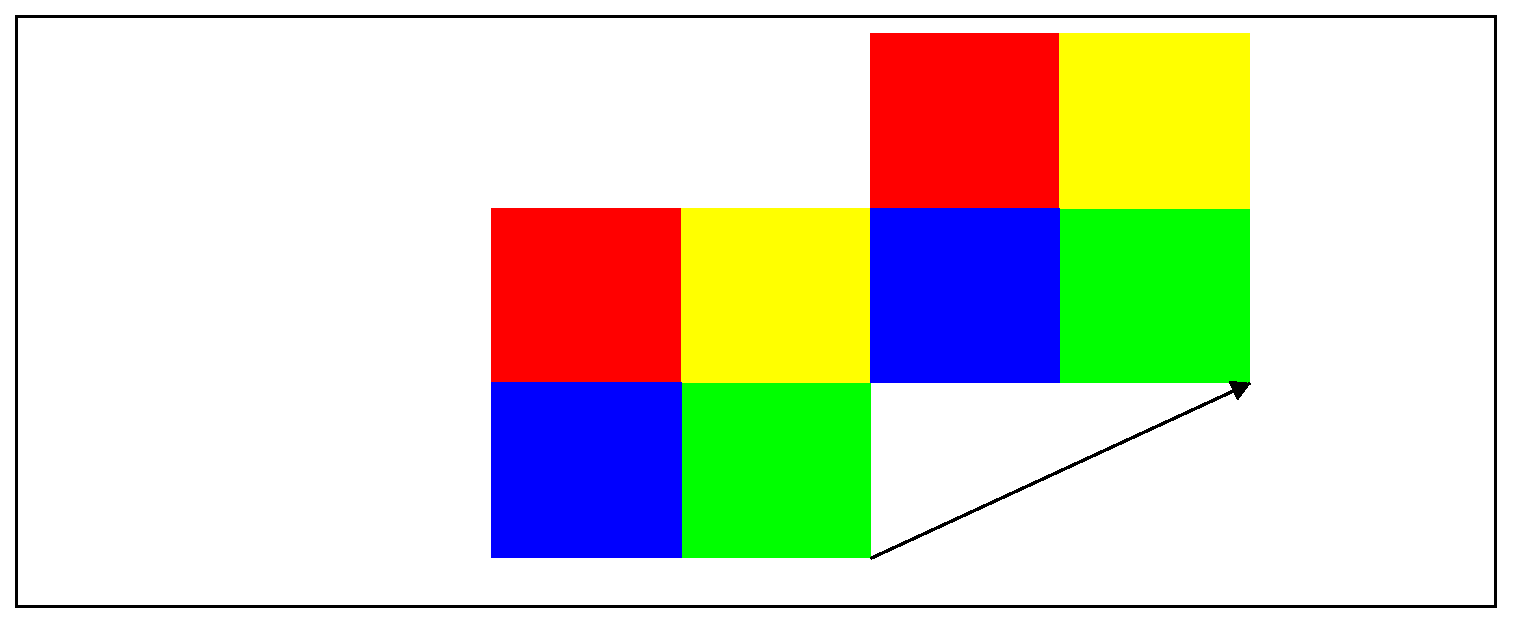
\includegraphics[width=\textwidth]{damiertrans1}\\
On tape :
\begin{verbatim}
C1:=carre(i,1+i,affichage=1+rempli);
translation(2+i,C1,affichage=1+rempli);
C2:=carre(1,2,affichage=2+rempli);
translation(2+i,C2,affichage=2+rempli);
C3:=carre(i+1,2+i,affichage=3+rempli);
translation(2+i,C3,affichage=3+rempli);
C4:=carre(0,1,affichage=4+rempli);
translation(2+i,C4,affichage=4+rempli);
translation(1+i,carre(0,1),affichage=4+rempli)
\end{verbatim}
On obtient :\\
\ \\
%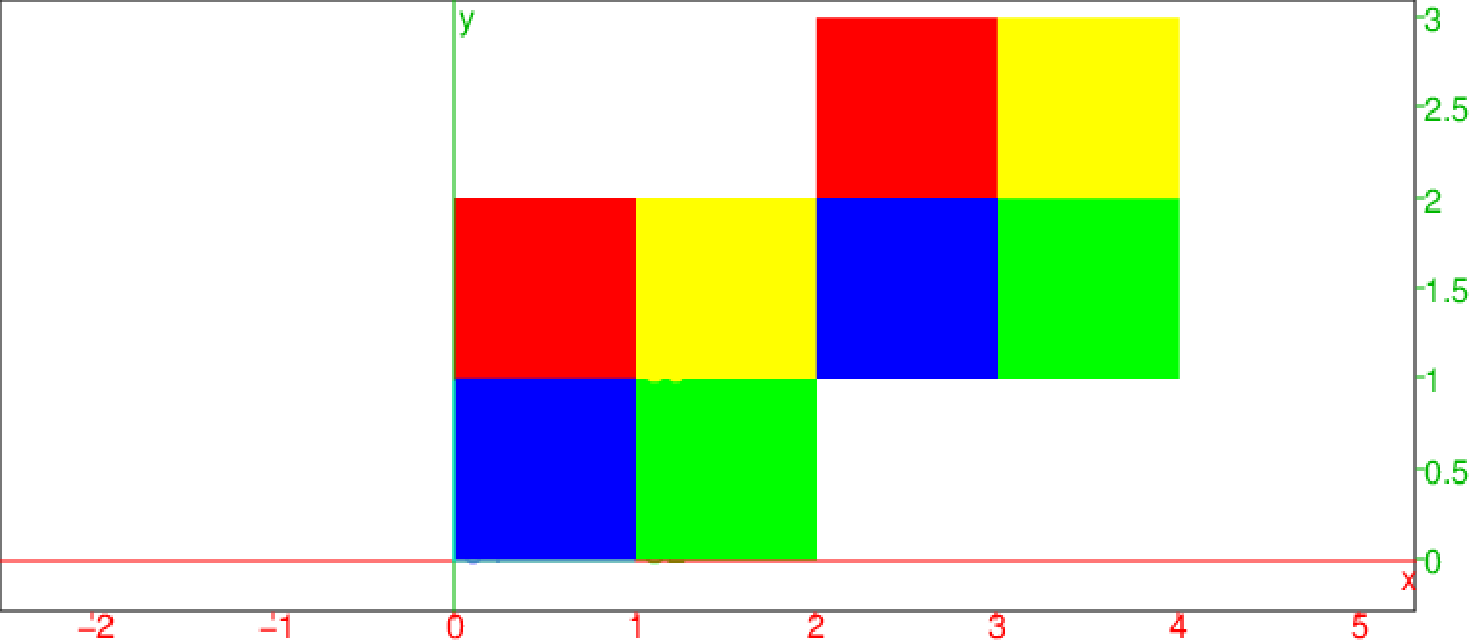
\includegraphics[width=\textwidth]{damiertrans}
%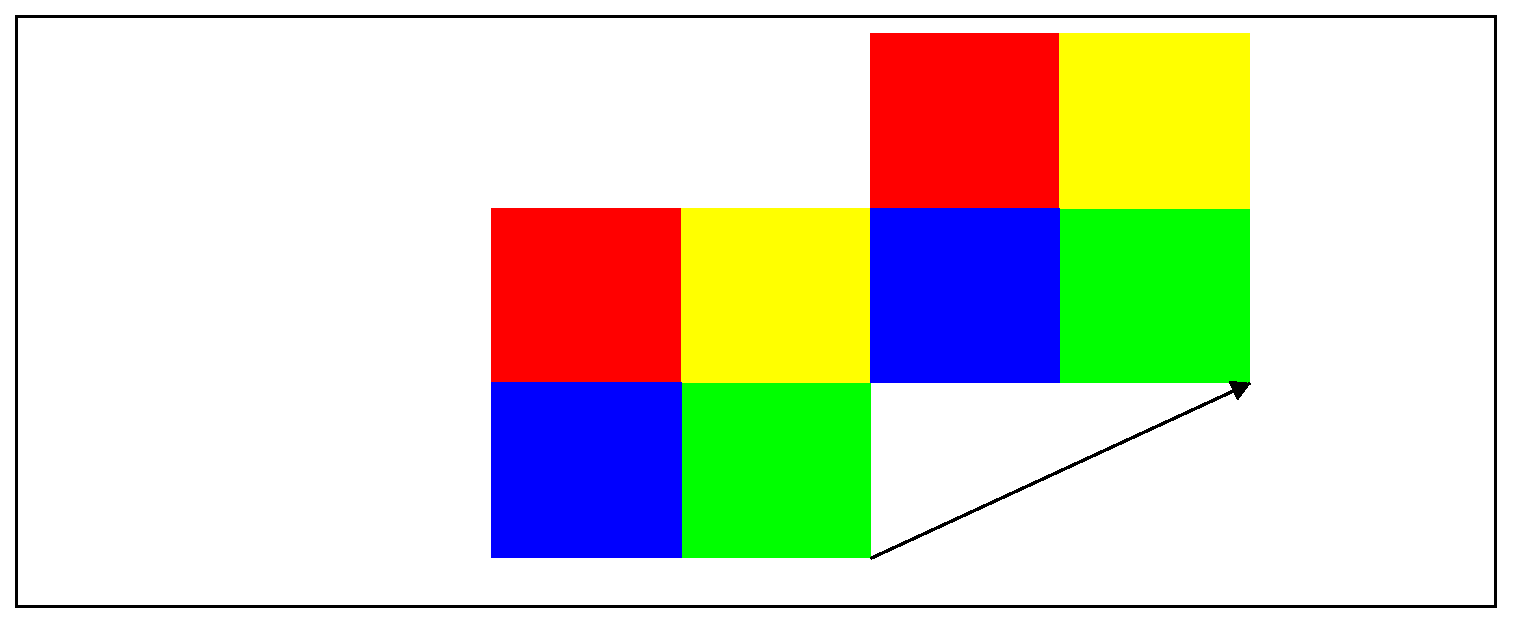
\includegraphics[width=\textwidth]{damiertrans1}
\subsection{La rotation}
{\bf D\'efinition}
Une rotation de centre $O$ et d'angle $t$ est une transformation 
ponctuelle qui, \`a un point $M$ fait correspondre un point $M'$ tel que :\\
$OM=OM'$ et $(\overrightarrow{OM},\overrightarrow{OM'}=t+2n\pi$ ($n\in \\Z$)\\
{\bf Propri\'et\'es}
Soient 2 points $A$ et $B$ et leurs transform\'es $A'$ et $B'$ par la 
rotation de centre $O$ et d'angle $t$. On a :\\
$AB=A'B'$ et $(\overrightarrow{AB},\overrightarrow{A'B'}=t+2n\pi$
La transform\'ee d'une droite est une droite.\\
Le transform\'e d'un cercle est un cercle de m\^eme rayon.\\
La rotation conserve les angles.\\
{\bf Avec Xcas}
{\tt rotation(O,t,M)} d\'esigne le transform\'e de $M$ dans la rotation de 
de centre, le point $O$, et d'angle $t$.\\
{\tt rotation(a+i*b,t,M)} d\'esigne le transform\'e de $M$ dans la rotation 
de centre, le point d'affixe $a+ib$, et d'angle $t$.\\
{\bf Une visualisation}
On consid\`ere la rotation de centre $C=(-2,0)$ et d'angle $\pi/3$.\\
On veut visualiser l'image par cette rotation des 4 carr\'es :
{\tt C1, C2, C3, C4}.\\
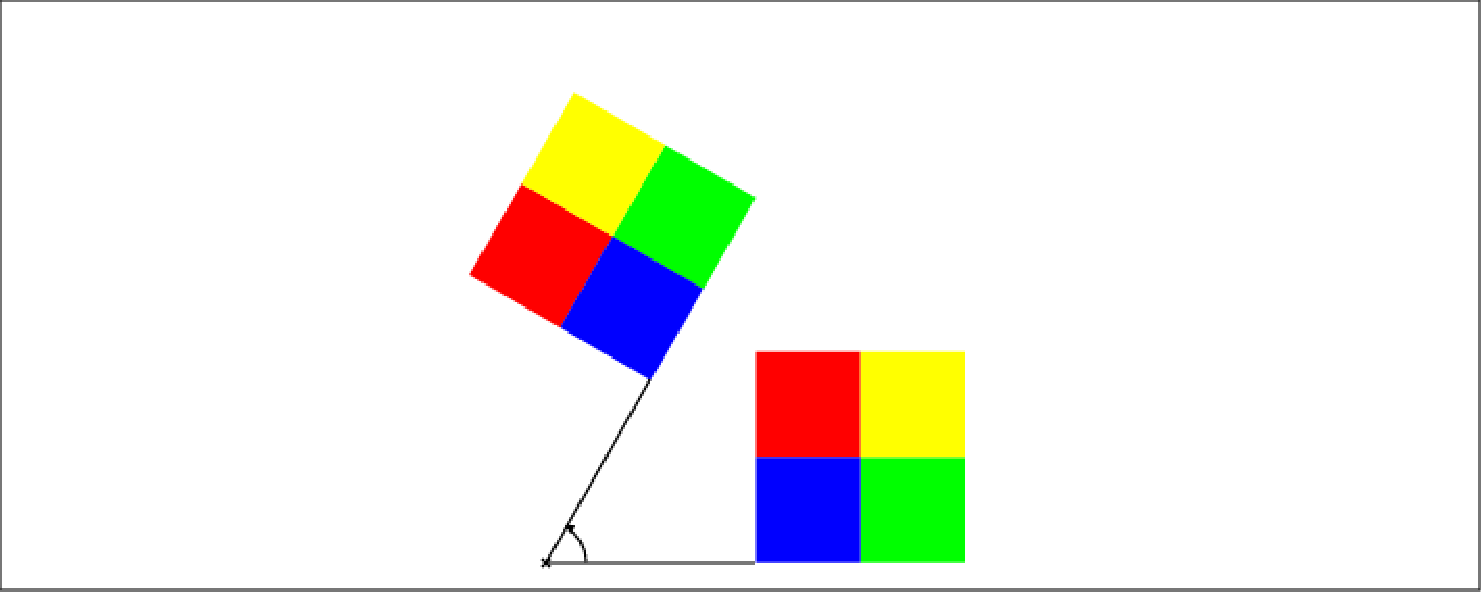
\includegraphics[width=\textwidth]{damierrot1}\\
On tape :
\begin{verbatim}
C1:=carre(i,1+i,affichage=1+rempli):;C1;
rotation(-2,pi/3,C1,affichage=1+rempli);
C2:=carre(1,2,affichage=2+rempli):;C2;
rotation(-2,pi/3,C2,affichage=2+rempli);
C3:=carre(i+1,2+i,affichage=3+rempli):;C3;
rotation(-2,pi/3,C3,affichage=3+rempli);
C4:=carre(0,1,affichage=4+rempli);
rotation(-2,pi/3,C4,affichage=4+rempli):;C4;
C:=point(-2);
O1:=rotation(C,pi/3,point(0)):;
segment(C,point(0),affichage=ligne_tiret_point));
segment(C,O1,affichage=ligne_tiret_point));
angle(C,point(0),O1,"pi/3");
\end{verbatim}
On obtient :\\
\ \\
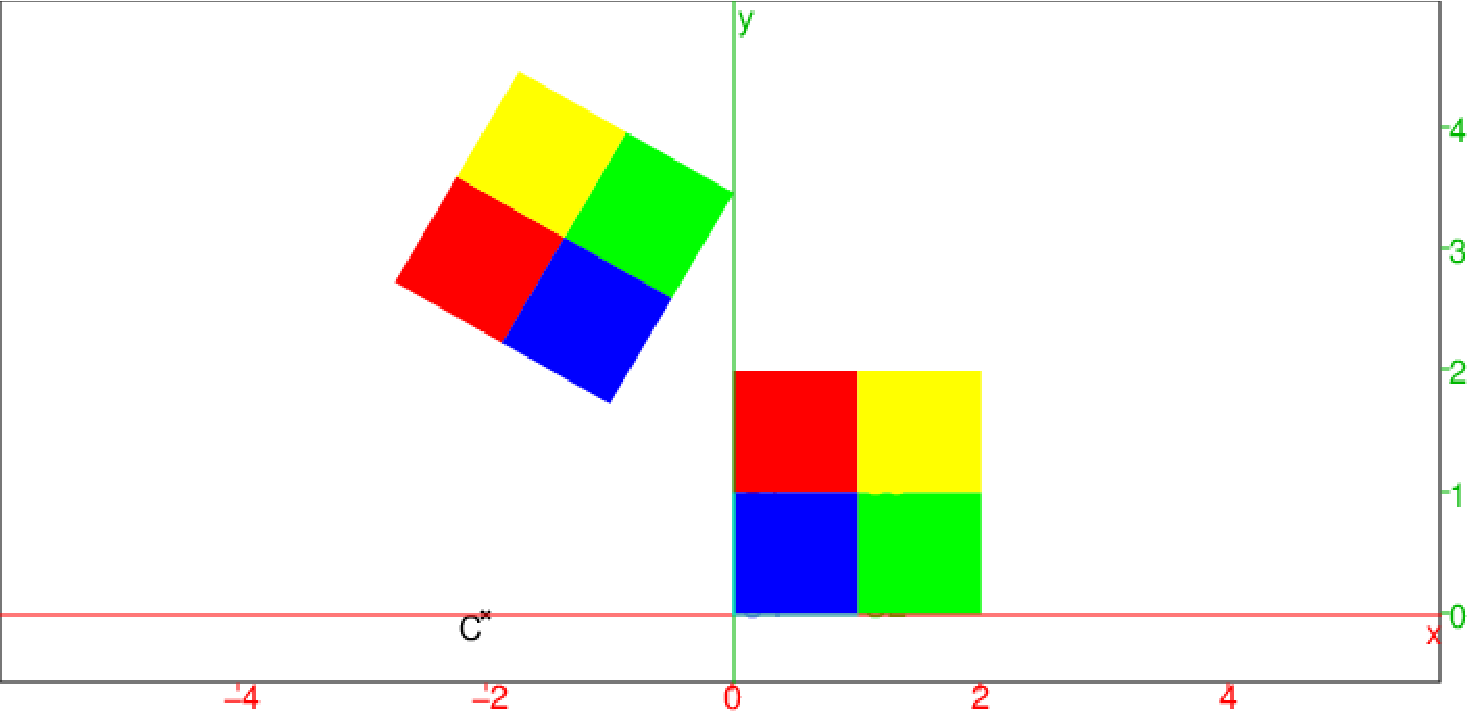
\includegraphics[width=\textwidth]{damierrot}
%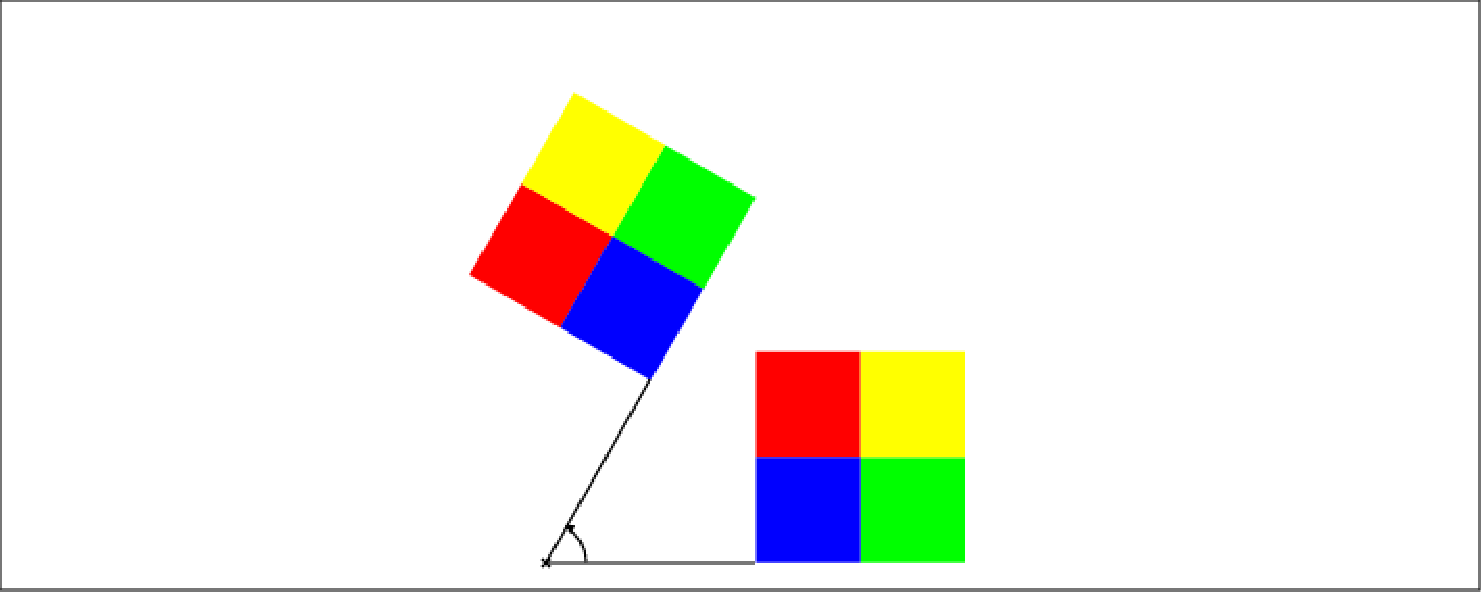
\includegraphics[width=\textwidth]{damierrot1}
{\bf Un exercice}\\
Sur les c\^ot\'es d'un triangle $ABC$ quelconque, on construit 3 carr\'es
$ACDE$, $BAFG$ et $BHIC$ puis 2 parall\'elogramme $BGJH$ et $CIKD$.\\
D\'emontrer que le triangle $AJK$ est rectangle isoc\`ele.\\
{\bf Une solution}\\
On fait la figure, on clique sur 3 points $A,B,C$ puis on tape :
\begin{verbatim}
triangle(A,B,C);
carre(A,C,D,E);
carre(C,B,H,I);
carre(B,A,F,G);
parallelogramme(H,B,G,J);
parallelogramme(D,C,I,K);
segment(A,J,affichage=1);
segment(A,K,affichage=1);
G1:=symetrie(B,G);
segment(B,G1,affichage=2);
segment(K,G1,affichage=2);
segment(K,C);
angle(C,I,K,"");angle(B,C,A,"");
angle(G,J,B,"");angle(K,D,C,"");
angle(D,C,K,"gamma");
angle(C,A,B,"gamma");
segment(B,J);
angle(J,B,G,"gamma");
segment(A,G);segment(A,G1);
\end{verbatim}
On obtient :\\
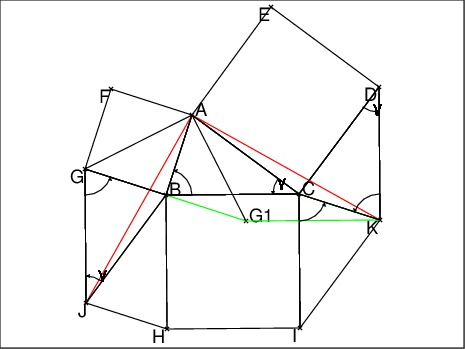
\includegraphics[width=\textwidth]{rectiso0}
On remarque tout d'abord que les triangles $BGJ$, $JHB$, $KCI$ et $CKD$ sont 
\'egaux au triangle $ABC$. En effet pour $BGJ$, on a $BG=AB$, $GJ=BC$ et 
l'angle $G$ est \'egale \`a $B$ comme angle \`a c\^ot\'es perpendiculaires.
donc le triangle $BGJ$ est \'egal \`a $ABC$.\\ 
De m\^eme $CKD$ est \'egal \`a $ABC$ l'angle $D$ est \'egale \`a $BC$ comme 
angle \`a c\^ot\'es perpendiculaires.\\
De plus $BGJ$ est aussi \'egal \`a $JHB$ et $CKD$  est aussi \'egal \`a $KCI$
puisque $BGJH$ et $CIKD$ sont des parall\'elogrammes.
Donc le triangle $BGJ$ est \'egal au triangle $KCI$, donc $CK$ est parall\`ele 
\`a $BG$. Si $G1$ est le sym\'etrique de $G$ par rapport \`a $B$ on en d\'eduit que le quadrilat\`ere $BG1KC$ est un parall\'elogramme.\\
On va chercher le transform\'e de $J$ par la rotation de centre $A$ et d'angle 
$+\pi/2$ si $ABC$ est direct et $-\pi/2$ sinon.
Supposons le triangle $ABC$ est direct.\\
La rotation de centre $A$ et d'angle $+\pi/2$ transforme $G$ en $G1$ et $J$ en 
$J1$. Le segment $G1J1$ a pour longueur $BC$ et est perpendiculaire \`a $GJ$ 
donc parall\`ele \`a $BC$.
$AGG1$ est un triangle rectanlgle isoc\`ele qui admet $AB$ comme bissectrice 
donc $G1$ est le sym\'etrique de $G$ par rapport \`a $B$.\\
Le quadrilat\`ere $BG1J1C$ est donc le parall\'elogramme $BG1KC$ et $J1$ et $K$
 sont confondus. Le triangle $AJK$ est donc rectangle isoc\`ele.
\subsection{La sym\'etrie droite et la sym\'etrie point}
{\bf D\'efinition}
La sym\'etrie par rapport \`a une droite $d$ est une transformation 
ponctuelle qui, \`a un point $M$ fait correspondre un point $M'$ tel que 
le segment $MM'$ soit perpendiculaire \`a $d$ en son milieu i.e.$d$ est la 
m\'ediatrice de $MM'$\\
La sym\'etrie par rapport \`a un point $O$ est une rotation de centre $O$ et 
d'angle $\pi$ (cf rotation pour les propri\'et\'es).\\
{\bf Propri\'et\'es de la sym\'etrie droite}
La transform\'ee d'une droite est une droite.\\
Le transform\'e d'un cercle est un cercle de m\^eme rayon.\\
La sym\'etrie transforme un angle en son oppos\'e.\\
{\bf Avec Xcas}
{\tt symetrie(droite(A,B),M)} ou {\tt symetrie(A,B,M)} d\'esigne le transform\'e
de $M$ dans la sym\'etrie par rapport \`a la droite $AB$.\\ 
{\tt symetrie(O,M)}  d\'esigne le transform\'e
de $M$ dans la sym\'etrie de centre $O$.\\ 
{\bf Une visualisation}
On consid\`ere la sym\'etrie par rapport \`a la droite passant par 
{\tt A:=point(0)} et {\tt B:= point(-1/2+i)}.\\
On veut visualiser l'image par cette sym\'etrie des 4 carr\'es :
{\tt C1, C2, C3, C4}.\\
On tape :
\begin{verbatim}
C1:=carre(i,1+i,affichage=1+rempli);
C2:=carre(1,2,affichage=2+rempli);
C3:=carre(i+1,2+i,affichage=3+rempli);
C4:=carre(0,1,affichage=4+rempli)
symetrie(droite(0,-1/2+i),C1,affichage=1+rempli);
symetrie(droite(0,-1/2+i),C2,affichage=2+rempli);
symetrie(droite(0,-1/2+i),C3,affichage=3+rempli);
symetrie(droite(0,-1/2+i),C4,affichage=4+rempli);
droite(0,-0.5+i)
\end{verbatim}
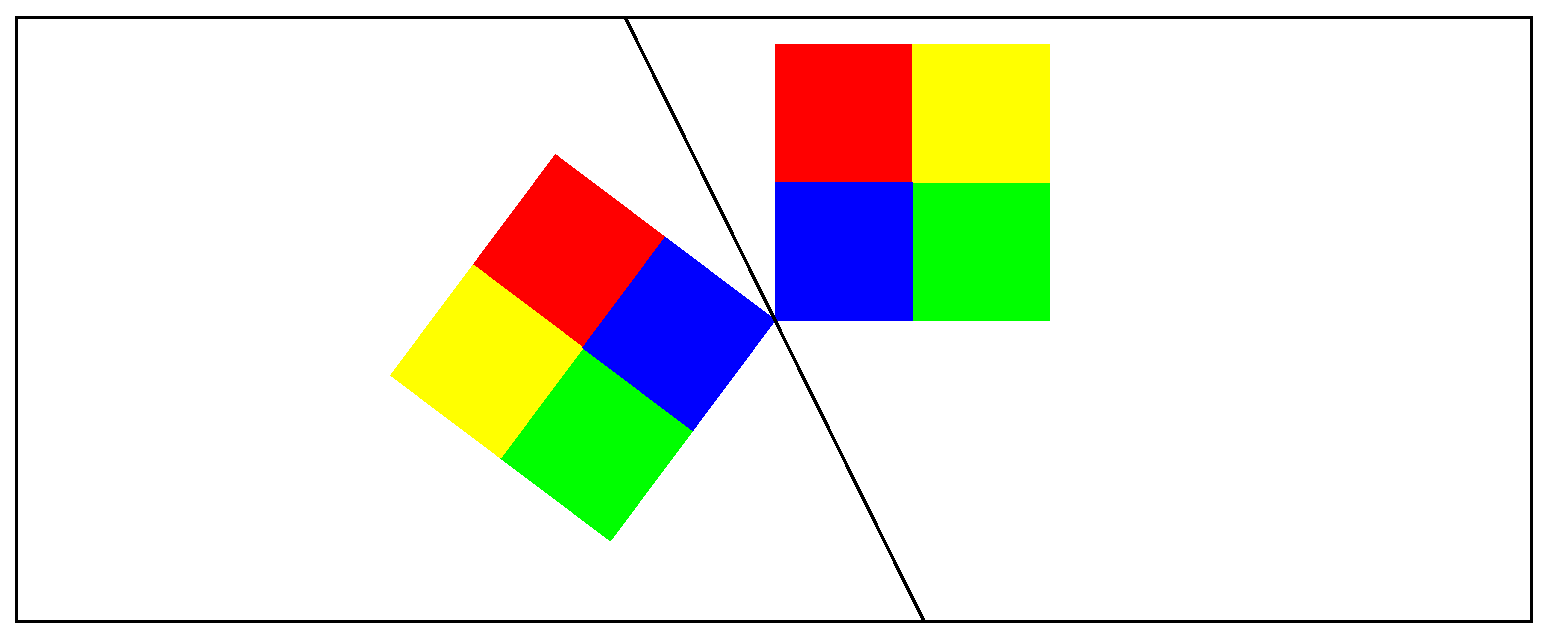
\includegraphics[width=\textwidth]{damiersym}
\subsection{L'homoth\'etie}
{\bf D\'efinition}
L'homoth\'etie de centre $O$ et de rapport $k$ est une transformation 
ponctuelle qui, \`a un point $M$ fait correspondre un point $M'$ tel que :\\
$\overrightarrow{OM'}=k\overrightarrow{OM}$\\
{\bf Propri\'et\'es}
Soient 2 points $A$ et $B$ et leurs transform\'es $A'$ et $B'$ par 
l'homoth\'etie de centre $O$ et de rapport $k$.
On a :\\
$\overrightarrow{A'B'}=k\overrightarrow{AB}$.\\
La transform\'ee d'une droite est une droite parall\`ele.\\
Le transform\'e d'un cercle de rayon $R$ est un cercle de rayon $kR$.\\
L'homoth\'etie conserve les angles.\\
{\bf Avec Xcas}
{\tt homothetie(O,k,M)} d\'esigne le transform\'e
de $M$ dans l'homoth\'etie de centre $O$ et de rapport $k$.\\
{\bf Une visualisation}
On consid\`ere la homoth\'etie de centre $C=(-2,0)$ et de rapport $1/2$.\\
On veut visualiser l'image par cette homoth\'etie des 4 carr\'es :
{\tt C1, C2, C3, C4}.\\
On tape :
\begin{verbatim}
C1:=carre(i,1+i,affichage=1+rempli);
homothetie(-2,1/2,C1,affichage=1+rempli);
C2:=carre(1,2,affichage=2+rempli);
homothetie(-2,1/2,C2,affichage=2+rempli);
C3:=carre(i+1,2+i,affichage=3+rempli);
homothetie(-2,1/2,C3,affichage=3+rempli);
C4:=carre(0,1,affichage=4+rempli);
homothetie(-2,1/2,C4,affichage=4+rempli);
C:=point(-2)
\end{verbatim}
On obtient :\\
\ \\
%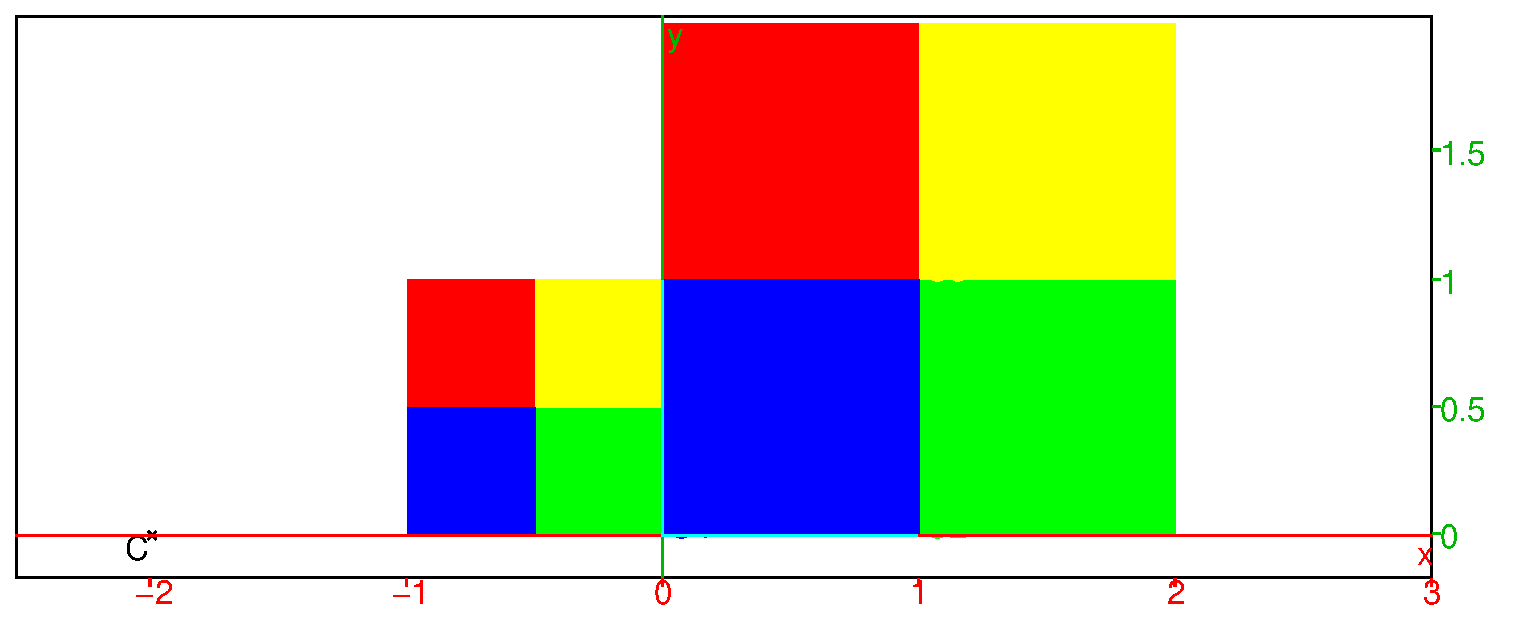
\includegraphics[width=\textwidth]{damierhomo}
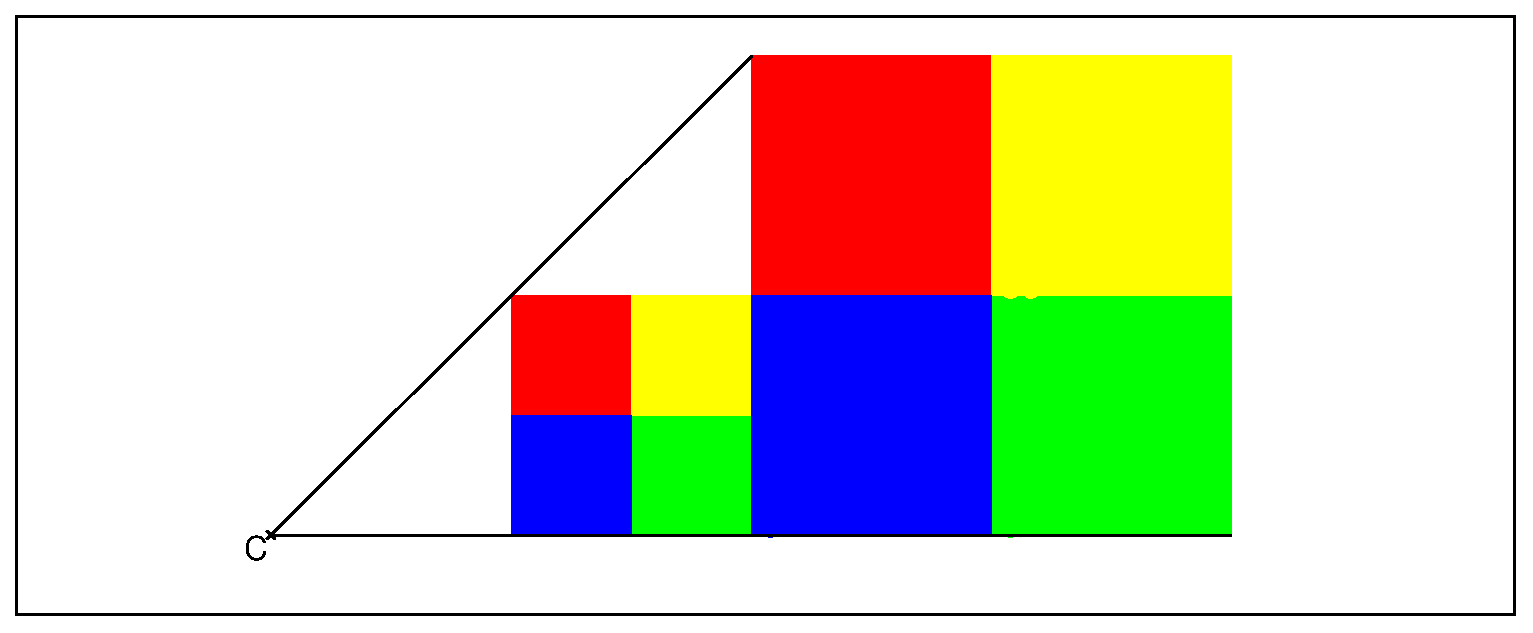
\includegraphics[width=\textwidth]{damierhomo1}
\subsection{La similitude}
{\bf D\'efinition}
La similitude de centre $O$, de rapport $k$ et d'angle $t$ est une 
transformation ponctuelle qui, \`a un point $M$ fait correspondre un point $M'$
tel que :\\
$OM'=k*OM$ et $(\overrightarrow{OM},\overrightarrow{OM'})=t$\\
{\bf Propri\'et\'es}
Soient 2 points $A$ et $B$ et leurs transform\'es $A'$ et $B'$ par 
la similitude de centre $O$ de rapport $k$ et d'angle $t$.
On a :\\
$A'B'=kAB$ et $(\overrightarrow{AB},\overrightarrow{A'B'})=t$.\\
La transform\'ee d'une droite est une droite.\\
Le transform\'e d'un cercle de rayon $R$ est un cercle de rayon $kR$.\\
La similitude conserve les angles.\\

{\bf Avec Xcas}
{\tt similitude(O,k,t,M)} d\'esigne le transform\'e
de $M$ dans la similitude de centre $O$, de rapport $k$ et d'angle $t$.\\
{\bf Une visualisation}
On consid\`ere la similitude de centre $C=(-2,0)$ et de rapport $1/2$ et d'angle 2*pi/3.\\
On veut visualiser l'image par cette similitude des 4 carr\'es :
{\tt C1, C2, C3, C4}.\\
On tape :
\begin{verbatim}
C1:=carre(i,1+i,affichage=1+rempli);
similitude(-2,1/2,2*pi/3,C1,affichage=1+rempli);
C2:=carre(1,2,affichage=2+rempli);
similitude(-2,1/2,2*pi/3,C2,affichage=2+rempli);
C3:=carre(i+1,2+i,affichage=3+rempli);
similitude(-2,1/2,2*pi/3,C3,affichage=3+rempli);
C4:=carre(0,1,affichage=4+rempli);
similitude(-2,1/2,2*pi/3,C4,affichage=4+rempli);
C:=point(-2)
\end{verbatim}
On obtient :\\
\ \\
%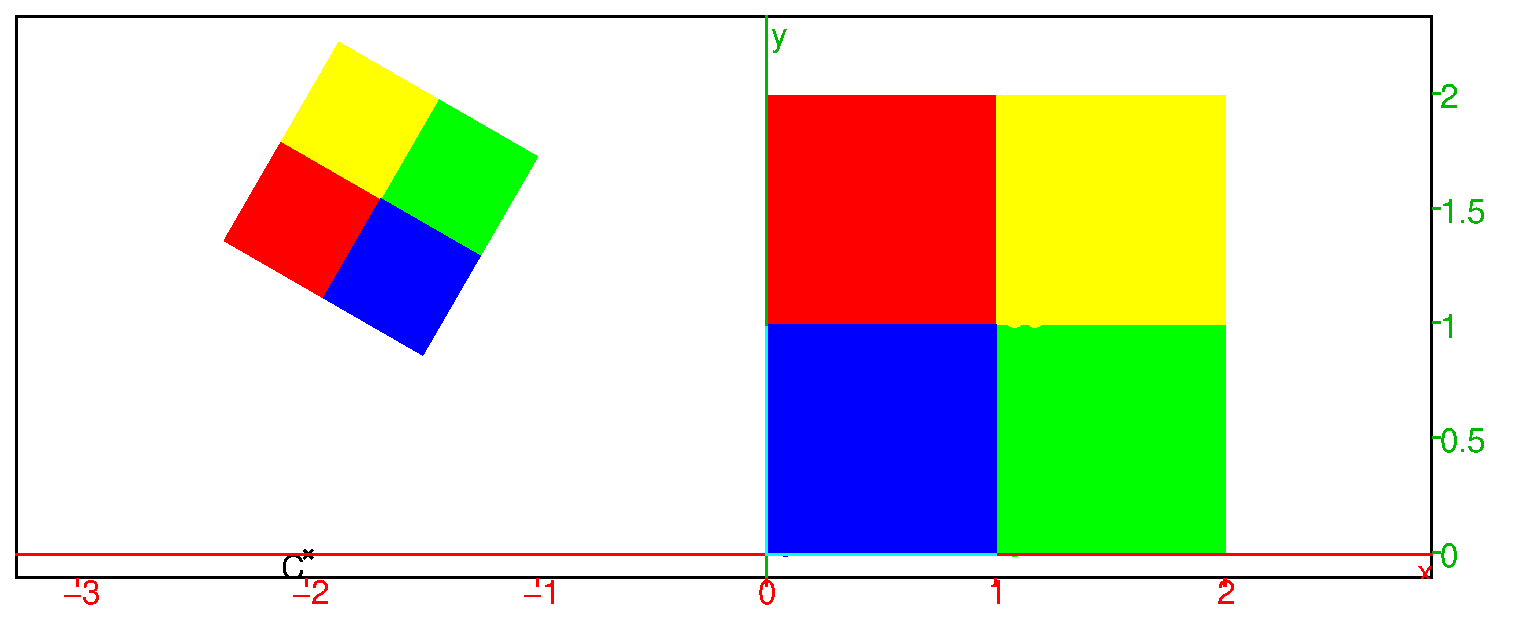
\includegraphics[width=\textwidth]{damiersimi}
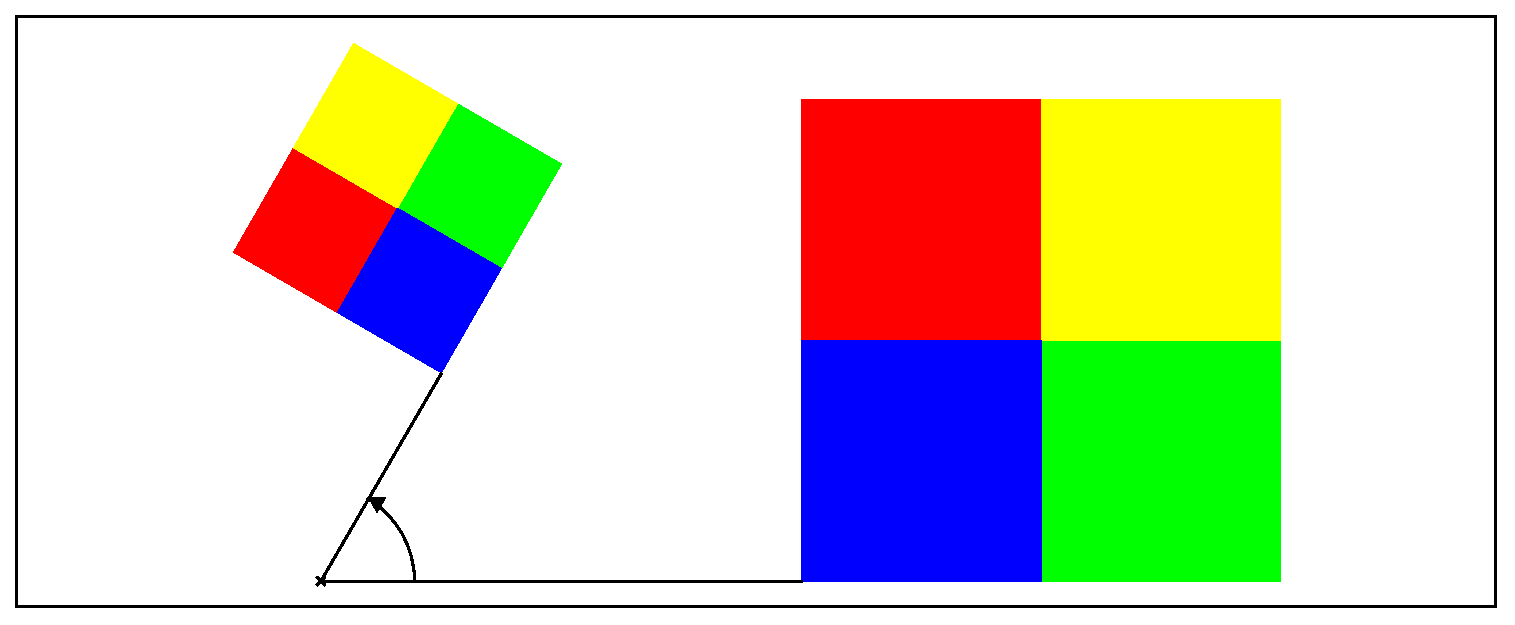
\includegraphics[width=\textwidth]{damiersimi1}
\subsection{L'inversion}
{\bf D\'efinition}
Une inversion de centre $C$ et de puissance $k$ est une transformation 
ponctuelle qui, \`a un point $M$ fait correspondre un point $M'$ tel que :\\
$\overline{OM}*\overline{OM'}=k$\\
{\bf Propri\'et\'es} 
Deux points quelconques et leurs inverses sont cocycliques ou sont align\'es 
avec le centre d'inversion.\\
L'inverse d'une droite passant par le centre d'inversion est elle-m\^eme.\\
L'inverse d'une droite ne passant pas par le centre d'inversion est un cercle
passant par le centre d'inversion dont le diam\`etre est perpendiculaire \`a
la droite.\\
{\bf Avec Xcas}
{\tt inversion(C,k,M)} d\'esigne le point inverse de $M$ dans l'inversion de 
centre $C$ et de puissance $k$.\\
{\bf Une visualisation}
On consid\`ere l'inversion de centre 0 et de puissance 1.\\
On veut visualiser l'image par cette inversion des 3 carr\'es :\\
{\tt carre(i,1+i,affichage=1+rempli),\\
 carre(i+1,2+i,affichage=3+rempli),\\
 carre(1,2,affichage=2+rempli)}\\
Pour pouvoir remplir une figure ayant comme contour des arcs de cercles on va
\'ecrire une proc\'edure qui trace les arcs avec des polygones.\\
On tape :
\begin{verbatim}
arcpoly(z0,r,a,b):={
return seq(z0+r*exp(i*t),t=a..b,0.05),z0+r*exp(i*b);
}:;
arccorde(z0,r,a,b,coul):={
local L;
L:=arcpoly(z0,r,a,b);
return polygone(L,affichage=coul+rempli)
}:;
arcpolyepais(z0,r,a,b,ep,coul):={
local L;  
L:=z0+(r-ep)*exp(i*a),z0+r*exp(i*a),arcpoly(z0,r,a,b),
  z0+(r)*exp(i*b),z0+(r-ep)*exp(i*b),arcpoly(z0,r-ep,b,a);
return affichage(polygone(L),c+rempli);
}:;  
\end{verbatim} 
Ainsi {\tt arccorde} dessinera la surface comprise entre l'arc et la corde avec
la couleur {\tt coul} et {\tt arcpolyepais} dessinera la surface comprise entre 
2 arcs, l'un de rayon {\tt r} et l'autre de rayon {\tt r-ep} avec la couleur 
{\tt coul}.\\
On tape :
\begin{verbatim}
triangle(1,1+i,i,affichage=4+rempli),
polygone(a1,a2,a3,affichage=1+rempli),
polygone(b1,b2,b3,affichage=2+rempli),
polygone(a2,b2,c1,c2,affichage=3+rempli),
carre(i,1+i,affichage=1+rempli),
carre(i+1,2+i,affichage=3+rempli),
carre(1,2,affichage=2+rempli),legende(0,"O")
\end{verbatim} 
On obtient :\\
\ \\
%\includegraphics[width=\textwidth]{invdamier}
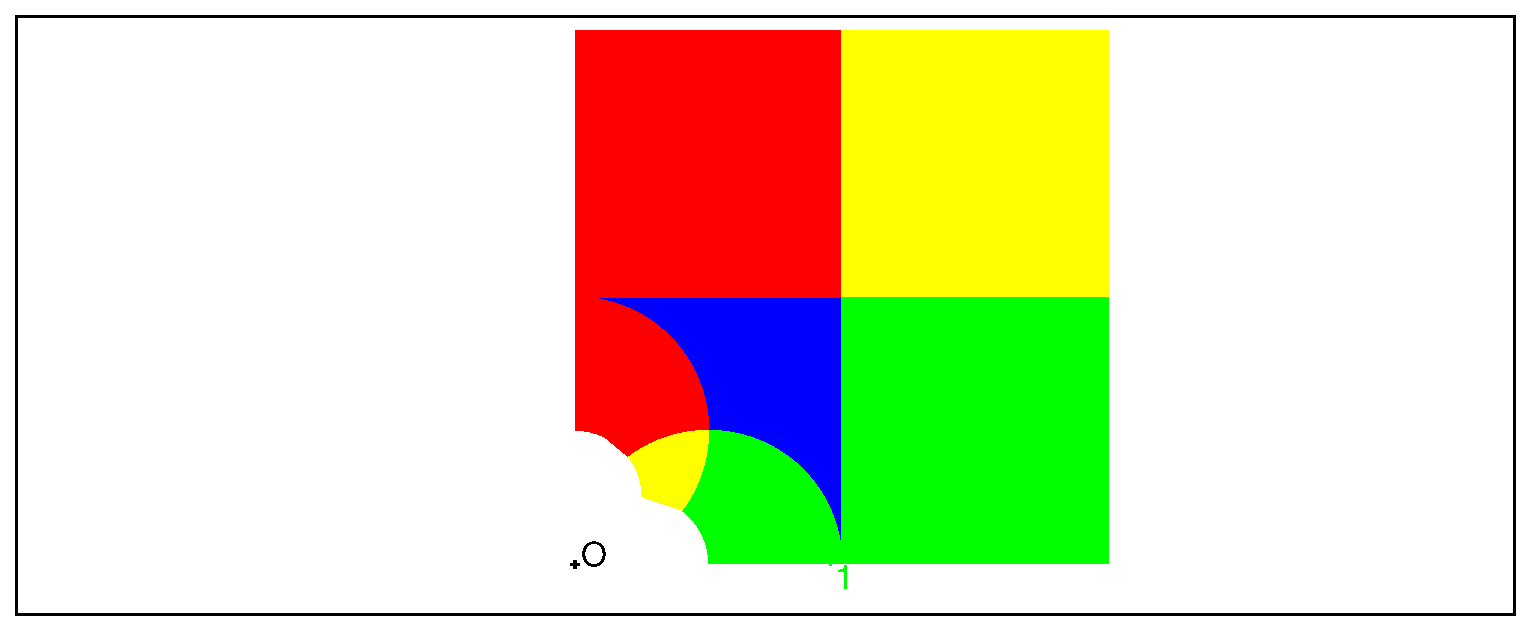
\includegraphics[width=\textwidth]{damierinv}
Les figures de m\^eme couleur sont inverses l'une de l'autre (en particulier 
les inverses des points de la figure bleue sont aussi dans la figure bleue qui 
est globalement invariante)
\section{}
\section{Le th\'eor\`eme de Pappus}
Voici les cercles de Pappus :\\
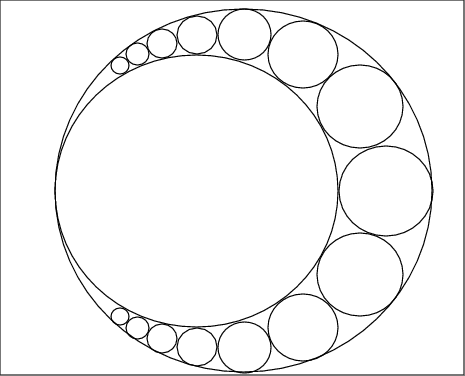
\includegraphics[width=\textwidth]{pappus1}
Th\'eor\`eme :\\
Si $\Gamma$ est le grand cercle de diam\`etre $b$, $C$ le cercle "moyen" de
diam\`etre $a$ ($a<b$) est tangent int\'erieurement \`a $\Gamma$ en $A$ et les 
petits cercles$c{_j},..c{_1},c_0,c_1..c_j$ sont tangents \`a $\Gamma$  et \`a 
$C$ et $c_j$ est tangent \`a $c_{j+1}$.\\ 
Les cercles $\Gamma$, $C$ et $c_0$  sont centr\'es sur la droite $D$.
Le th\'eor\`eme de Pappus dit que si $r_j$ et le rayon de $c_j$ et si $d_j$ est
la distance du centre de $c_j$ \`a $D$ alors $d_1=2r_1$ et $d_j=2*j*r_j$ pour 
$j=0..n$.\\ 
De plus les points de tangences des cercles $c_j$ et $c_{j+1}$ sont sur un 
cercle de diam\`etre $2\frac{ab}{a+b}$, tangent en $A$ \`a $\Gamma$ et $C$.
{\bf Construction des cercles de Pappus.}\\
On va utiliser une inversion qui transforme $\Gamma$ et $C$ en 2 droites 
parall\`eles $d_1$ et $d_2$. Cette inversion aura comme centre le point $A$ 
commun \`a  $\Gamma$ et $C$. Les cercles $c_k$ seront transform\'es en des 
cercles qui seront tangents \`a ces 2 droites : les transform\'es seront donc 
des cercles \'egaux. et les points de tangences de ces cercles sont sur la 
parall\`ele \'equidistante \`a $d_1$ et $d_2$.\\
Voici la fonction qui renvoie le transform\'e d'un cercle $c$, son centre et 
son rayon (lorsque ce transform\'e est un cercle) par l'inversion de centre $A$
et de puissance $k$ :
\begin{verbatim}
inversionc(A,k,c):={
  local p,O1,r1,O,r,B,B1;
  O:=centre(c);
  r:=rayon(c);
  si est_element(A,c) alors
    B:=symetrie(O,A);
    B1:=inversion(A,k,B);
  return perpendiculaire(B1,droite(O,A)); fsi;
  si A==O alors return cercle(O,k/r),O,k/r; fsi;
  p:=puissance(c,A);//p:=longueur2(A,O)-r^2
  r1:=k*r/p;
  O1:=inversion(A,k,projection(polaire(c,A),A));
  return cercle(O1,r1),O1,r1;
  }:;
\end{verbatim} 
on a 
$r_1=k*r/(AO^2-r^2)$
$O_1$ est l'inverse du point d'affixe
$(r^2+(xA-i*yA)*(xO+i*yO)-(xO^2+yO^2))/(xA-xO+(-i)*(yA-yO))$
On tape :\\
\begin{verbatim}
k:=24;
Gamma:=cercle(point(2),2):;Gamma;
C:=cercle(point(3/2),3/2):;C;
d1:=inversionc(0,k,Gamma):;d1;
d2:=inversionc(0,k,C):;d2[0];
c0:=cercle(point(6),point(8));
c1:=cercle(7+2*i,1):;
C0:=inversionc(point(0),k,c0);;C0[0];
C1:=inversionc(point(0),k,c1):;C1[0];
L:=cercle(7+2*k*i,1)$(k=-7..7):;L;
L1:=inversionc(0,k,L[j])$(j=0..14):;L1[0];
\end{verbatim} 

On obtient :\\
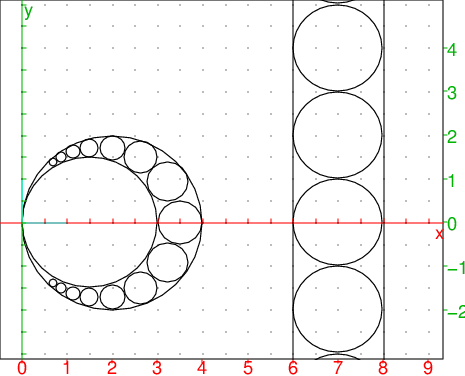
\includegraphics[width=\textwidth]{pappus2}\\

{\bf D\'emonstration du th\'eor\`eme de Pappus avec {\tt Xcas}}
On prend comme origine $A$ le centre de l'inversion, et comme axe des $x$ la 
droite  des centres.\\
$\Gamma$ est le cercle de diam\`etre {\tt A point(b)} et $C$ est le cercle de 
diam\`etre {\tt A point(a)}.\\
$\Gamma$ se transforme par l'inversion de centre $A$ et de puissance $k$ en la 
droite d'\'equation $x=k/b$\\
$C$ se transforme par l'inversion de centre $A$ et de puissance $k$ en la 
droite d'\'equation $x=k/a$\\
Le cercle des points de tangence des cercles $c_j$ est donc le transform\'e par
l'inversion de centre $A$ et de puissance $k$ de la droite d'\'equation 
$x=(k/b+k/a)/2=k(a+b)/(2ab)$ c'est donc le cercle de diam\`etre 
{\tt A point(2a*b/(a+b))}.\\
Le cercle $c0$ est de diam\`etre $AB$ et son transform\'e $C0$
dans l'inversion de centre $A$ et de puissance $k$ a pour centre
{\tt point(k/2*(1/a+1/b))} et comme rayon {\tt r:=k/2*(1/a-1/b)}.\\
On consid\`ere donc le  cercle $C_j$ de rayon 
{\tt r:=k/2*(1/a-1/b)} et de centre {\tt oj:=point(k/2*(1/a+1/b)+i*2*j*r);} 
Soit $c_j$ l'inverse de $C_j$ dans 
l'inversion de centre $A$ et de puissance $k$.\\
On cherche l'ordonn\'ee du centre et du rayon de $c_j$.\\
On tape :
\begin{verbatim}
A:=point(0);
assume(a=[3,0,10,0.1]);
assume(b=[4,a,10,0.1]);;
cercle(A,point(a));
cercle(A,point(b));
supposons(k=[23.9,0,25,0.1]);
c0:=cercle(point(a),point(b));
C0:=inversionr(A,k,c0);
supposons(j=[1,0,7,1]);
r:=k/2*(1/a-1/b);
oj:=point(k/2*(1/a+1/b)+i*2*j*r);
Cj:=cercle(oj,r);
cj:=inversionr(A,k,Cj);
cj[0];
dj:=simplify(ordonnee(cj[1]));
rj:=simplify(ordonnee(cj[1])/cj[2]);
simplify(ordonnee(dj/rj);
\end{verbatim}
On obtient pour $dj$ :\\
{\tt (-a\verb|^|2*b*j+a*b\verb|^|2*j)/(a\verb|^|2*j\verb|^|2-2*a*b*j\verb|^|2+a*b+b\verb|^|2*j\verb|^|2)}\\
On obtient pour $rj$ :\\
{\tt(-a\verb|^|2*b+a*b\verb|^|2)/(2*a\verb|^|2*j\verb|^|2-4*a*b*j\verb|^|2+2*a*b+2*b\verb|^|2*j\verb|^|2)}\\
On obtient pour $dj/rj$ :\\
{\tt (2*j}\\
Donc {\tt Xcas} a d\'emontr\'e que $d_j=2jr_j$.

\section{Un probl\`eme de partage}
\subsection{Le probl\`eme}
Un p\`ere poss\`ede un terrain triangulaire. Il veut forer un puits \`a 
l'int\'erieur de son terrain, de fa\c{c}on qu'\'a sa mort chacun de ses 3 fils 
poss\`ede un morceau triangulaire de m\^eme surface ayant acc\`es au puits.

Soit $ABC$ le terrain initial et $P$ l'emplacement du puits.\\
Chaque fils aura comme morceau $ABP$ ou $APC$ ou $BCP$ et ces morceaux 
doivent avoir m\^eme aire qui est le tiers de l'aire de  $ABC$.\\
Donc la hauteur de $ABP$ doit \^etre le tiers de la hauteur de $ABC$ issue de 
$C$ et la hauteur de $BCP$ doit \^etre le tiers de la hauteur de $ABC$ issue de
$A$.\\
Avec {\tt Xcas} on clique sur 3 points et on 
tape dans un \`ecran de g\'eom\'etrie :\\
\begin{verbatim}
triangle(A,B,C);
I:=A+(C-A)/3;
dc:=parallele(I,droite(B,A));
J:=A+2*(C-A)/3;
da:=parallele(J,droite(B,C));
P:=inter_unique(da,dc);
affichage ([segment(P,A),segment(P,B),segment(P,C)],rouge)
K:=B+(A-B)/3
\end{verbatim}
On obtient :\\

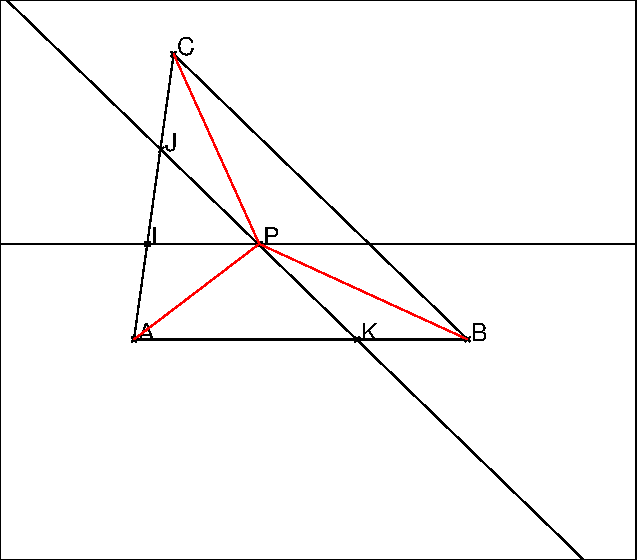
\includegraphics[width=\textwidth]{triangle}

On tape pour v\'erifier :\\
{\tt aire(A,B,P),aire(B,C,P),aire(C,A,P)}\\

Propri\'et\'es du point {\tt P}\\
{\tt I} est le milieu de {\tt AJ}, {\tt IP} est parall\`ele \`a {\tt AK} 
donc {\tt P} est le milieu de {\tt KJ}.
{\tt AP} est une m\'ediane de {\tt AKJ}, {\tt KJ} est parall\`ele \`a {\tt BC}
donc {\tt AP} est une m\'ediane de {\tt ABC}.\\
On montrerait de m\^eme que {\tt BP} et {\tt CP} sont des m\'edianes de 
{\tt ABC}.\\
{\tt P} est donc le centre de gravit\'e du triangle {\tt ABC} ou encore
l'isobarycentre des 3 points {\tt A,B,C}.\\
On tape pour v\'erifier :\\
{\tt affichage(isobarycentre(A,B,C),point\_width\_2)}
\subsection{G\'en\'eralisation du probl\`eme}
Un p\`ere poss\`ede un terrain triangulaire et a $n$ fils ($n=3,4,5...$).\\ 
Il veut forer un puits \`a l'int\'erieur de son terrain, de fa\c{c}on qu'\'a sa 
mort,  chacun de ses $n$ fils poss\`ede un morceau triangulaire de m\^eme 
surface ayant acc\`es au puits. D\'eterminer le nombre de solutions possibles.

Pour $n=4$, on cherche 2 points {\tt P} et {\tt D} avec {\tt D} 
par exemple sur {\tt BC} (il y a donc 3 solutions selon que l'on choisit
{\tt D} sur {\tt BC} ou  sur {\tt AC} ou  sur {\tt AB}) 
pour que chaque fils ait comme morceau $ABP$ ou $APC$ ou $BDP$ ou $DCP$
et que ces morceaux soient de  m\^eme aire \`a savoir le quart de l'aire de  
$ABC$.\\
Avec {\tt Xcas} on clique sur 3 points et on 
tape dans un \`ecran de g\'eom\'etrie :\\
\begin{verbatim}
triangle(A,B,C);
I:=A+(C-A)/4;
dc:=parallele(I,droite(B,A));
J:=A+(C-A)/2;
da:=parallele(J,droite(B,C));
P:=inter_unique(da,dc);
D:=milieu(B,C);
affichage ([segment(P,A),segment(P,B),segment(P,C),
            segment(P,D)],rouge);
K:=B+(A-B)/2;
\end{verbatim}
 
On obtient :\\

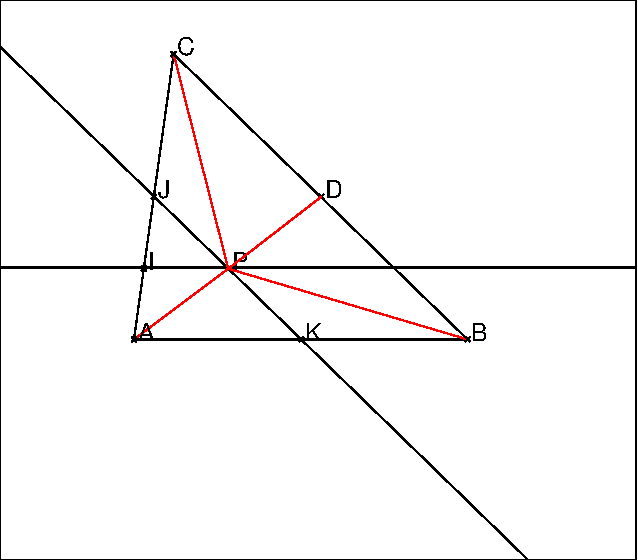
\includegraphics[width=\textwidth]{triangle4}

On tape pour v\'erifier :\\
{\tt aire(A,B,P),aire(B,D,P),aire(C,A,P),aire(D,C,P)}\\

Propri\'et\'es du point {\tt P}\\
{\tt I} est le milieu de {\tt AJ}, {\tt IP} est parall\`ele \`a {\tt AK} 
donc {\tt P} est le milieu de {\tt KJ}.
{\tt AP} est une m\'ediane de {\tt AKJ}, {\tt KJ} est parall\`ele \`a {\tt BC}
donc {\tt AP} est la  m\'ediane {\tt AD} de {\tt ABC}.\\
De plus {\tt P} est le milieu de {\tt AD} puisque {\tt J} est le milieu de 
{\tt AC}, {\tt JP} est parall\`ele \`a {\tt DC} .\\
{\tt P} est donc le barycentre des 3 points {\tt [A,2],[B,1],[C,1]}.\\
On tape pour v\'erifier :\\
{\tt affichage(barycentre([A,2],[B,1],[C,1]),point\_width\_2)}.\\
Les 2 autres solutions, pour l'emplacement du puits, sont obtenues avec :\\
{\tt affichage(barycentre([A,1],[B,2],[C,1]),point\_width\_2)}\\
{\tt affichage(barycentre([A,1],[B,1],[C,2]),point\_width\_2)}\\

Pour $n=5$, on cherche 3 points {\tt P, D} et {\tt E} avec {\tt D et E} sur un 
m\^eme c\^ot\'e par exemple sur {\tt BC} ou {\tt D} et {\tt E} sur des 
c\^ot\'es diff\'erents par exemple {\tt D} sur {\tt BC} et {\tt E} 
par exemple sur {\tt AC} (il y a donc en tout 6 solutions : 3 solutions selon 
que l'on choisit {\tt D} et {\tt E} sur {\tt BC} ou  sur {\tt AC} ou  sur 
{\tt AB} et 3 solutions selon que l'on choisit {\tt D} et {\tt E} pas sur 
{\tt BC} ou pas sur {\tt AC} ou pas sur {\tt AB}) 
pour que chaque fils ait comme morceau un triangle de sommets pris parmi
{\tt A,B,C,D,E,P}
et que ces morceaux soient de  m\^eme aire \`a savoir le cinqui\`eme de l'aire 
de  
$ABC$.\\
Avec {\tt Xcas} on clique sur 3 points et on 
tape dans un \`ecran de g\'eom\'etrie :\\
\begin{verbatim}
triangle(A,B,C);
I:=A+(C-A)/5
dc:=parallele(I,droite(B,A));
J:=A+2*(C-A)/5;
da:=parallele(J,droite(B,C));
P:=inter_unique(da,dc);
D:=B+(C-B)/3;
E:=B+2*(C-B)/3;
affichage ([segment(P,A),segment(P,B),segment(P,C),
            segment(P,D),segment(P,E)],rouge)
K:=B+3*(A-B)/5;
affichage(barycentre([A,3],[B,1],[C,1]),point_width_2);
\end{verbatim}
On obtient :\\

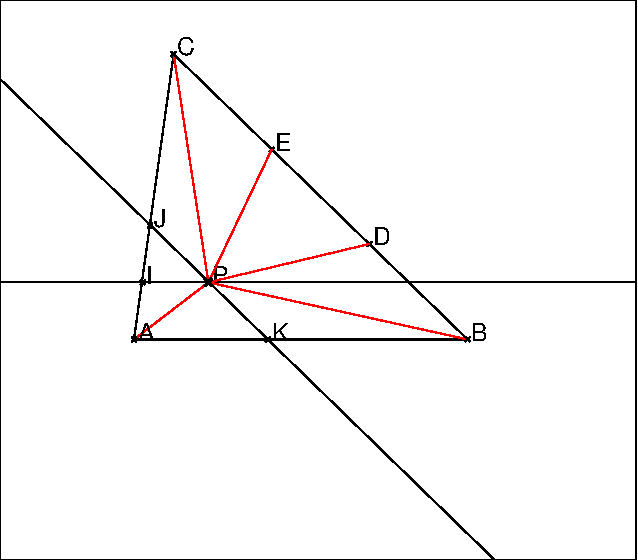
\includegraphics[width=\textwidth]{triangle5}

On tape pour v\'erifier :\\
{\tt aire(A,B,P),aire(B,D,P),aire(C,A,P),aire(D,E,P),aire(E,C,P)}\\

Propri\'et\'es du point {\tt P}\\
{\tt I} est le milieu de {\tt AJ}, {\tt IP} est parall\`ele \`a {\tt AK} 
donc {\tt P} est le milieu de {\tt KJ}.
{\tt AP} est une m\'ediane de {\tt AKJ}, {\tt KJ} est parall\`ele \`a {\tt BC}
donc {\tt AP} est la  m\'ediane de {\tt ABC}.\\
De plus {\tt P} est situ\'e au 2/5 de cette m\'ediane de {\tt AD} puisque 
{\tt J} est situ\'e au 2/5 de {\tt AC}, {\tt JP} est parall\`ele \`a {\tt DC}.\\
Donc l'aire de {\tt PBC} vaut les 3/5 de l'aire de {\tt ABC}
{\tt P} est donc le barycentre des 3 points {\tt [A,3],[B,1],[C,1]}.\\
On tape pour v\'erifier :\\
{\tt affichage(barycentre([A,2],[B,1],[C,1]),point\_width\_2)}.\\
On voit le partage en rouge sur la figure lorsque le puits est en {\tt P}.\\
Les 2 autres solutions, pour l'emplacement du puits lorsque l'on choisit 
{\tt D} et {\tt E} sur le m\^eme c\^ot\'e, sont obtenues avec :\\
{\tt affichage(barycentre([A,1],[B,2],[C,1]),point\_width\_2)}\\
{\tt affichage(barycentre([A,1],[B,1],[C,2]),point\_width\_2)}\\
Les 3 autres solutions, pour l'emplacement du puits lorsque l'on choisit 
{\tt D} et {\tt E} sur des c\^ot\'es, sont obtenues avec :\\
{\tt affichage(barycentre([A,2],[B,2],[C,1]),point\_width\_2)}\\
{\tt affichage(barycentre([A,2],[B,1],[C,2]),point\_width\_2)}\\
{\tt Q:=affichage(barycentre([A,1],[B,2],[C,2]),point\_width\_2)}\\ 
On voit le partage en vert sur la figure lorsque le puits est en {\tt Q} :\\

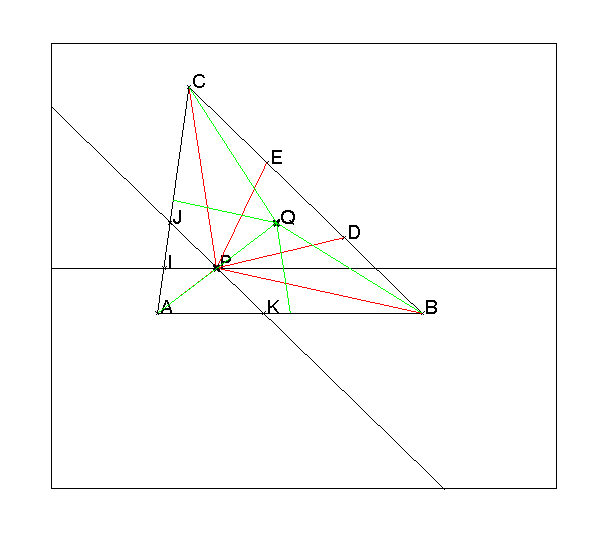
\includegraphics[width=\textwidth]{triangles5}

On g\'en\'eralise ais\'ement.\\
On montre par r\'ecurrence que le nombre de solutions pour $n$ ($n>3$) est : 
$(n-2)(n-1)/2$.\\
En effet on cherche le nombre de triplets d'entiers non nuls de somme $n$ i.e.
on cherche le nombre de triplets $(a,b,c)\in \mathbb N^{*3}$ v\'erifiant 
$a+b+c=n$.
pour $n=3$ ce nombre est 1=$(n-2)(n-1)/2$ car (1+1+1=3)\\
{\bf Hypoth\`ese de recurrence} : pour $n$ ce nombre est $(n-2)(n-1)/2$, \\
pour $n+1$, on cherche le nombre de 
triplets d'entiers non nuls de somme $n+1$ :\\
si $a+b+c=n+1$, c'est que $a+b<n+1$ car $c \neq 0$\\
Donc le probl\`eme revient \`a chercher le nombre de couples $(a,b)$ d'entiers 
non nuls de somme strictement inf\'erieure \`a $n+1$. Par hypoth\`ese de 
recurrence, le nombre de couples $(a,b)$ d'entiers 
non nuls de somme strictement inf\'erieure \`a $n$ est $(n-2)(n-1)/2$. Il reste
donc \`a comptabiliser les couples $(a,b)$ d'entiers 
non nuls de somme $n$ : il y en $n-1$ puisque $a$ peut prendre $n-1$ valeurs. 
Donc le nombre de triplets d'entiers non nuls de somme $n+1$ est :\\
$(n-2)(n-1)/2+n-1=(n-1)(n-2+2)/2=(n-1)n/2$.
On a ainsi montrer par r\'ecurrence que le nombre de solutions pour le partage
en $n$ triangles de m\^eme aire est $(n-2)(n-1)/2$.\\
Il est interessant de voir alors la disposition des diff\'erents puits les uns 
par rapport aux autres : il forme un reseau triangulaire de c\^ot\'e $n-2$
et on retrouve alors le nombre de puits avec la formule :\\
$1+2+...+(n-2)=(n-2)(n-1)/2$.
\section{Le sigle CE}
Il existe une diff\'erence subtile entre le sigle CE "Comformit\'e Europ\'eenne"
indiquant que le produit r\'epond \`a des normes de s\'ecurit\'e et qu'il peut 
circuler librement en Europe et le sigle CE signifiant "China Export".\\
Seul l'espace entre le C et le E et diff\'erent : dans le sigle chinois le C et
le E sont plus proches.\\
Alors  soyez vigilant !
\subsection{Le sigle "Comformit\'e Europ\'eenne"}
On tape :
\begin{verbatim}
cercle(-5,5);
cercle(-5,4);
cercle(4,5);
cercle(4,4);
c1:=cercle(-5,5,pi/2,3*pi/2,affichage=rempli);
c2:=cercle(-5,4,pi/2,3*pi/2,affichage=rempli+ 7);
c3:=cercle(4,5,pi/2,3*pi/2,affichage=rempli);
c4:=cercle(4,4,pi/2,3*pi/2,affichage=rempli+ 7);
rectangle(i/2,-i/2,4,affichage=rempli);
papier_quadrille(1,pi/2,x=-11..10,y=-6..6);
\end{verbatim}
On obtient :\\
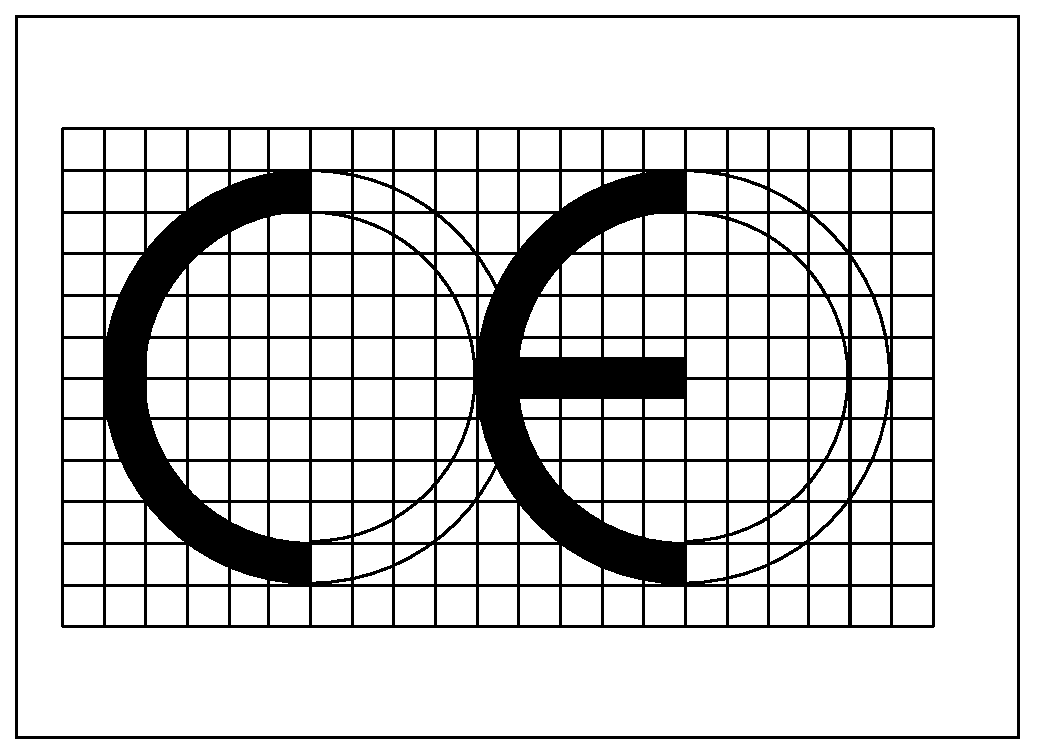
\includegraphics[width=\textwidth]{siglecee}
\subsection{Le sigle "China Export"}
On tape :
\begin{verbatim}
cercle(1,5);
cercle(1,4);
c1:=cercle(-5,5,pi/2,3*pi/2,affichage=rempli);
c2:=cercle(-5,4,pi/2,3*pi/2,affichage=rempli+ 7);
c5:=cercle(1,5,pi/2,3*pi/2,affichage=rempli);
c6:=cercle(1,4,pi/2,3*pi/2,affichage=rempli+ 7);
rectangle(-3+i/2,-3-i/2,4,affichage=rempli);
papier_quadrille(1,pi/2,x=-11..10,y=-6..6);
cercle(-5,5);
cercle(-5,4);
\end{verbatim}
On obtient :\\
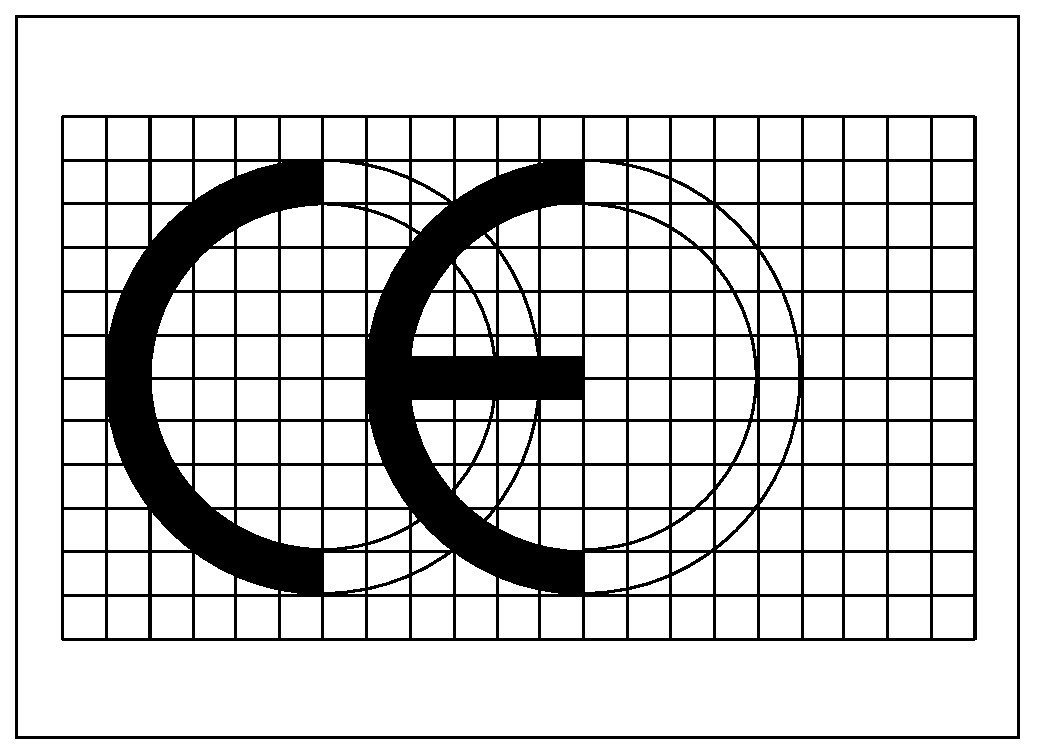
\includegraphics[width=\textwidth]{siglecec}
\section{Le cercle inscrit}
\subsection{Le probl\`eme}
Soient $ABC$ un triangle et $M$ un point qui se d\'eplace sur le segment $BC$.
Soit $I$ (resp $J$) le centre du cercle inscrit au triangle $ABM$ (resp $ACM$).
Montrer que le cercle de diam\`etre $IJ$ passe par un point fixe lorsque
le point $M$ se d\'eplace sur le segment $BC$.

\subsection{Les lemmes}
\subsubsection{Lemme1}
Soient $c$ est un cercle de diam\`etre $AB$ et une corde $MP$ avec $M$ et $P$ 
situ\'e d'un m\^eme c\^ot\'e de $AB$.
Soient $A1$ et $B1$ les projections respectives de $A$ et $B$ sur $MP$.\\
Alors 
$$\overrightarrow{A1M}=\overrightarrow{PB1}$$
\begin{center}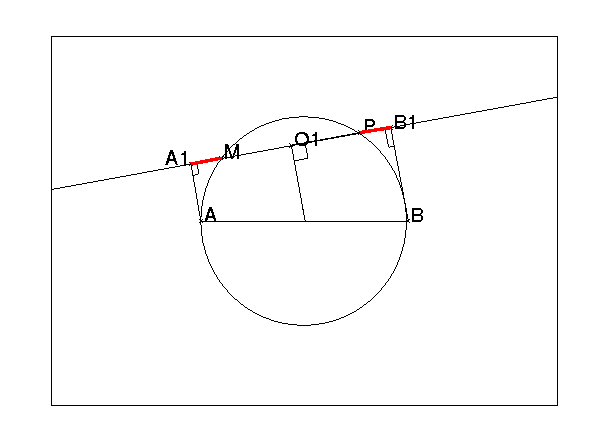
\includegraphics[width=8cm]{inscrit1}\end{center}

En effet le centre de $c$ est le milieu de $AB$ et donc il se projette sur le 
milieu de $MP$. Comme le milieu de $AB$ se projette sur le 
milieu $O1$ de $A1B1$, on a $A1B1$ et $MP$ ont m\^eme milieu.\\
Donc  :
$$\overrightarrow{A1M}=\overrightarrow{A1O1}+\overrightarrow{O1M}=\overrightarrow{O1B1}+\overrightarrow{PO1}=\overrightarrow{PB1}$$

\subsubsection{Lemme2}
Soient $ABC$ un triangle et $K$ le centre de son cercle inscrit.\\
Alors $K$ est le barycentre des points $[A,a],[B,b],[C,c]$ o\`u $a,b,c$ sont 
les longueurs des c\^ot\'es $BC$, $AC$, $AB$.\\

\begin{center}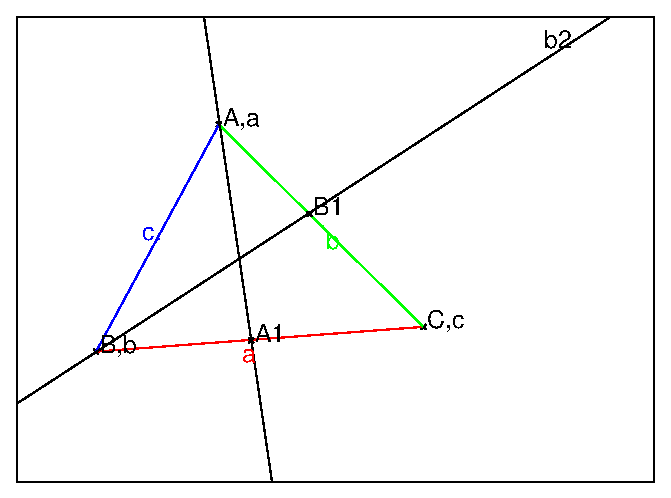
\includegraphics[width=8cm]{inscrit2}\end{center}
Si la bissectrice int\'erieure de l'angle $A$ coupe $BC$ en $A1$ on a :
$A1B/A1C=c/b$ donc $b*A1B=c*A1C$ ou encore puisque $A1$ se trouve sur le 
segment $BC$ :
$$b*\overrightarrow{A1B}+c*\overrightarrow{A1C}=0$$
donc $A1$ est le barycentre de $[B,b],[C,c]$.

Si la bissectrice int\'erieure de l'angle $B$ coupe $AC$ en $B1$ on a :
$B1A/B1C=c/a$ donc $a*B1A=c*B1C$ ou encore puisque $B1$ se trouve sur le 
segment $AC$ :
$$a*\overrightarrow{B1A}+c*\overrightarrow{B1C}=0$$
donc $B1$ est le barycentre de $[A,a],[C,c]$.\\
Donc le barycentre des points $[A,a],[B,b],[C,c]$ est l'intersection de 
$AA1$ et de $BB1$ c'est \`a dire l'intersection des bissectrices $K$ 
qui est le centre du cercle inscrit.

\subsubsection{Lemme3}
Soient un triangle $ABC$ et $K1$ un point de la droite $BC$.\\
Alors $K1$ est la projection sur $BC$ du centre du cercle inscrit \`a $ABC$ si 
et seulement si :
$$K1B-K1C=AB-AC$$
\begin{center}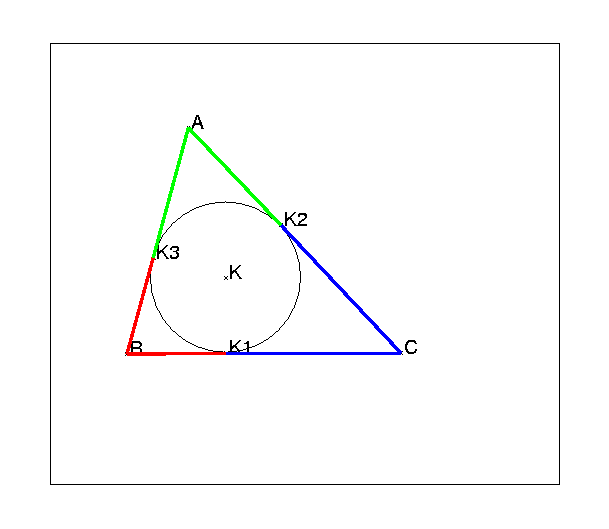
\includegraphics[width=10cm]{inscrit3}\end{center}
Soit $K$ le centre du cercle inscrit \`a $ABC$.\\
Soient $K1,\ K2$ et $K3$ les projections respectives de $K$ sur $BC,\ AC$ et 
$AB$.
Puisque les c\^ot\'es $AB,AC,BC$ sont des tangentes au cercle inscrit et que
$K1,K2,K3$ sont les points de contact de ces tangentes, on a :
$$BK1=BK3,\ CK1=CK2,\ AK2=AK3$$ et 
$K1,\ K2$ et $K3$ se trouvent respectivement sur les segments sur $BC,\ AC$ et
$AB$.
Donc :
$$AB-AC=AK3+K3B-(AK2+K2C)=K1B-K1C$$

Soit $K1$ tel que $K1B-K1C=AB-AC$.\\
Le point $K1$ se trouve sur le segment $BC$ en effet si $K1$ \'etait \`a 
l'exterieur de $BC$ on aurait $|K1B-K1C|=|BC|>|AB-AC|$ d'apres l'in\'egalit\'e 
triangulaire ce qui condredit l'hypoth\`ese $K1B-K1C=AB-AC$.
L'\'egalit\'e $K1B-K1C=AB-AC$ d\'efinit un seul point $K1$ du segment $BC$, ce 
point est donc la projection du centre du cercle inscrit \`a $ABC$
\subsection{La solution g\'eom\'etrique}
Pour la solution g\'eom\'etrique, on va se servir des lemmes 1 et 3.
La bissectrice de l'angle $BMA$ et la bissectrice de l'angle $ CMA$ sont perpendiculaire donc $M$ est sur le cercle de diam\'etre $IJ$.
Ce cercle  coupe le segment $BC$ en $M$ et $P$. Montrons que $P$ est fixe.
Soient $I1$ et $J1$ les projections de $I$ et $J$ sur $BC$.

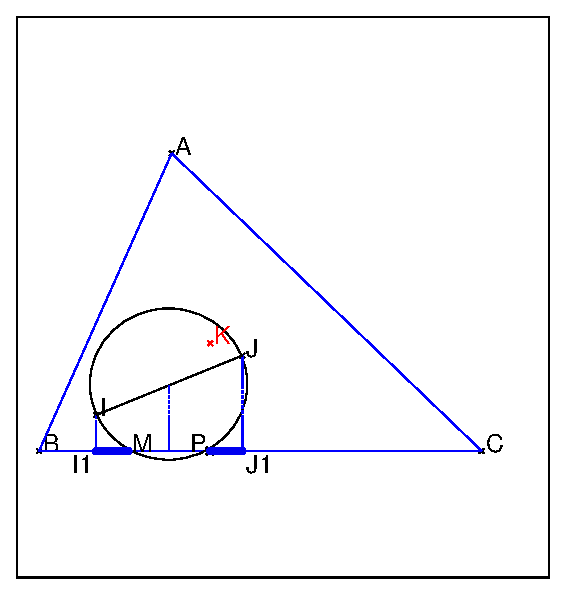
\includegraphics[width=\textwidth]{inscritcalc}\\
%D'apr\`es le {\bf\ lemme1\} on a :
%$$\overrightarrow{I1M}=\overrightarrow{PJ1}$$
D'apr\`es le {\bf\ lemme3\ } on a :\\
$I1B-I1M=AB-AM$ et\\
$J1M-J1C=AM-AC$ donc
$$I1B-I1M+J1M-J1C=AB-AM+AM-AC=AB-AC$$
Puisque $I1$ et $J1$ sont entre $B$ et $C$, et que $M$ et $P$ sont entre
$I1$ et $J1$, on a  $M$ et $P$ sont entre $B$ et $C$.\\
D'apr\`es le {\bf lemme1} on a :\\
$\overrightarrow{I1M}=\overrightarrow{PJ1}$ et 
$\overrightarrow{I1P}=\overrightarrow{MJ1}$ donc
$$I1B-I1M+J1M-J1C=I1B-PJ1+I1P-J1C$$
$M$ et $P$ sont entre $B$ et $C$ donc
$I1B+I1P=PB$ et $PJ1+J1C=PC$ d'o\`u :
$$PB-PC=AB-AC$$
Le point $P$ est fixe et $P$ est la projection du centre $K$ du cercle inscrit
\`a $ABC$.
\subsection{La solution avec {\tt Xcas}}
Le choix des param\`etres est important !
Sans perte de g\'en\'eralit\'e, on peut prendre l'origine du rep\`ere en $B$,
et $C$ sur l'axe des $x$ d'abscisse $a$. Le point $M$ est donc sur l'axe des 
$x$ d'abscisse $m<a$ .\\
Si on choisit comme param\`etres les coordonn\`ees  de $A$, {\tt Xcas} n'arrive
pas \`a faire les calculs (cf la remarque ci-apr\`es). Mais si on choisit comme param\`etres les longueurs 
$b$ et $c$ des c\^ot\'es $AC$ et $AB$ les calculs sont simples m\^eme si
on ne d\'efinit pas les centres des cercles inscrits comme des barycentres :
on peut indiff\'erement mettre pour d\'efinir $I$ :\\
{\tt I:=barycentre([A,m],[B,l1],[M,c]);} (cf {\bf lemme2}) ou\\
{\tt I:=normal(centre(inscrit(A,B,M)));} (idem pour d\'efinir $J$ et $K$)
On tape :
\begin{verbatim}
B:=point(0);
supposons(a=[1,0,2,0.1]);
C:=point(a);
supposons(b=[0.9,0,2,0.1]);
supposons(c=[1.1,0,2,0.1]);
A:=inter(cercle(B,c),cercle(C,b))[1];
triangle(A,B,C);
supposons(m=[0.4,0,a,0.1]);
M:=point(m);
b1:=longueur(A,M);
I:=barycentre([A,m],[B,b1],[M,c]);
J:=barycentre([A,a-m],[C,b1],[M,b]);
K:=barycentre([A,a],[B,b],[C,c],affichage=1);
I1:=projection(droite(y=0),I,affichage=quadrant3);
J1:=projection(droite(y=0),J,affichage=quadrant4);
K1:=projection(droite(y=0),K,affichage=quadrant2+
                               epaisseur_point_2);
\end{verbatim}
On obtient :
\begin{center}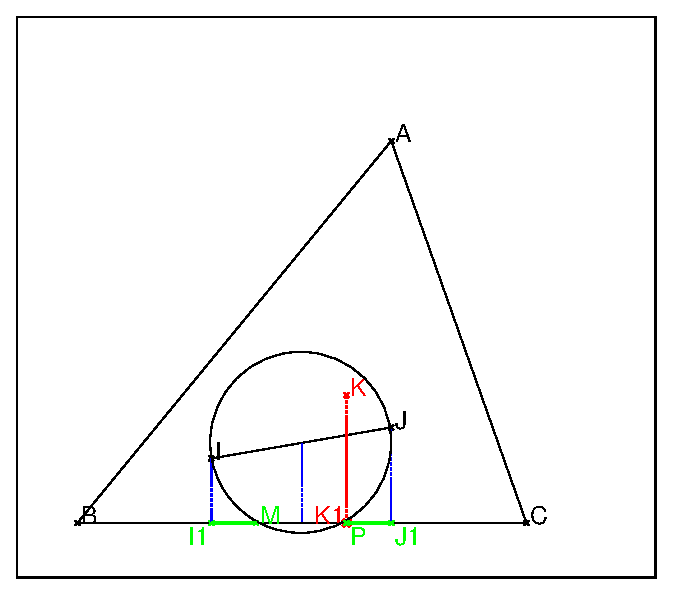
\includegraphics[width=9cm]{inscritabc}\end{center}
On tape :
\begin{center}{\tt simplify(2*longueur(B,K1)-a))}\end{center}
On obtient :
\begin{center}{\tt -b+c}\end{center}
cela prouve le {\bf lemme3} puisque $CK1=a-BK1$ on a :
$$BK1-CK1=2*BK1-a=c-b=AB-AC$$
On tape en se servant du {\bf lemme1} pour d\'efinir $P$ :
\begin{center}{\tt P:=I1+vecteur(M,J1):;}\end{center}
\begin{center}{\tt simplify(affixe(P))}\end{center}
On obtient :
\begin{center}{\tt (a-b+c)/2}\end{center}
Donc $P$ est fixe.\\
On tape :
\begin{center}{\tt simplify(affixe(K1))}\end{center}
On obtient :
\begin{center}{\tt  (a-b+c)/2}\end{center}
Donc $P$ et $K1$ sont confondus.

{\bf Remarque}
On peut aussi faire faire le calcul \`a {\tt Xcas} avec au d\'epart plus de 
param\`etres que n\'ecessaire et donner ensuite les relations entre ces 
param\`etres seulement \`a la fin des calculs.\\
On choisit comme param\`etres :\\
$a1$ l'abscisse de $A$,\\
$a$ l'abscisse de $C$,\\
$m$ l'abscisse de $M$,\\
$b1$ la longueur de $AM$,\\
$b$ la longueur de $AC$,\\
$c$ la longueur de $AB$.\\
$\cos(B)$ le cosinus de l'angle $B$ qu triangle $ABC$
Ces param\`etres v\'erifient :\\
$a1=c*\cos(B)$\\
$b1^2=m^2+c^2-2m*c*cos(B)$\\
$b^2=c^2+a^2-2a*c*\cos(B)$\\
Si on note $i1$ l'affixe de $I1$, $j1$ l'affixe de $J1$ et $p1$ l'affixe de 
$P1$, on a, avec les notations pr\'ec\'edentes, $PB-PC=2*PB-a$.\\
On tape :
\begin{verbatim}
i1:=affixe(barycentre([point(a1),m],[point(0),b1],[point(m),c]));
j1:=affixe(barycentre([point(a1),a-m],[point(m),b],[point(a),b1]));
p1:=simplify(i1+j1-m);
res:=simplify(2*p1-1);
res:=simplify(subst(subst(res,[a1=c*cos(B),b1^2=m^2+c^2-2*m*c*cos(B)]),
            cos(B)=(-b^2+c^2+a^2)/(2*c*a)));
\end{verbatim}
On obtient alors facilement pour $PB-PC=2*PB-a$={\tt res} :\\
{\tt -b+c}\\
Donc  $PB-PC=c-b=AB-AC$.

\section{Un probl\`eme de surface minimum}
Ce probl\`eme a \`ete donn\'e aux olympiades acad\'emiques de 2005.
\subsection{Le probl\`eme}
Soit une feuille de papier rectangulaire $ABCD$ de c\^ot\'es $AB=4$ unit\'es 
et $BC=6$ unit\'es.
Soient $R$ un point du segment $AB$ et, $T$ un point du segment 
$CB$. $R$ et $T$ sont tels que si on plie la feuille selon le segment $RT$ 
le point $B$ se trouve sur le segment $AD$. On appelle $S$ le point du segment
$AD$ qui coincide avec $B$ lors du pliage.\\
On pose $AR=a$ et $BT=b$.\\
\begin{itemize}
\item Trouver les valeurs minimales et maximales de $a$,
\item Trouver une relation entre $a$ et $b$,
\item Trouver la valeur de $a$ pour laquelle l'aire de $BRT$ est minimale.
\end{itemize}
\subsection{La figure}
On peut faire la figure \`a l'aide d'une feuille de papier que l'on plie de 
fa\c{c}on \`a amener le coin $B$ de la feuille sur $AD$ ou bien, on utilise 
{\tt Xcas} mais alors :
\begin{itemize}
\item on peut d\'efinir tout d'abord $S$, puis d\'efinir la 
pliure comme la m\'ediatrice $m$ de $BS$, puis on trouve les points $R$ et $T$
comme intersection de $m$ avec les segments $AB$ et $BC$.\\
Gr\^ace \`a {\tt s:=element(0..6);S:=point(s*i);} on peut faire bouger le point
$S$ sur $AD$.\\
On tape (voir {\tt minis.xws}) :
\begin{verbatim}
A:=point(0);
B:=point(4);
C:=point(4+6*i);
D:=point(6*i);
quadrilatere(A,B,C,D);
assume(s=[2,0,6]);
S:=point(s*i);
m:=mediatrice(B,S);
R:=inter_unique(m,droite(A,B));
T:=inter_unique(m,droite(C,B));
equation(m);
r:=coordonnees(R);
t:=normal(coordonnees(T));
AT:=aire(triangle(R,B,T));
\end{verbatim}
On obtient :\\

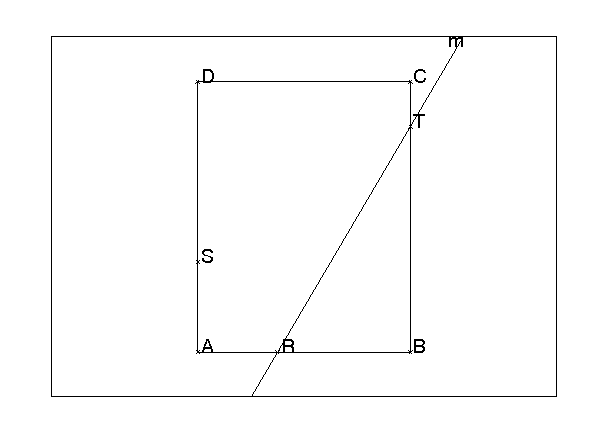
\includegraphics[width=\textwidth]{minis}
\item on peut d\'efinir tout d'abord $R$ d'abscisse $a$, puis d\'efinir le 
point $S$ comme intersection du cercle de centre $R$ et de rayon $4-a$ avec le
segment $AD$, puis la pliure comme la m\'ediatrice $m$ de $BS$,
 
On tape  (voir {\tt minia.xws}):
\begin{verbatim}
A:=point(0);
B:=point(4);
C:=point(4+6*i);
D:=point(6*i);
quadrilatere(A,B,C,D);
assume(a=[1,0,4]);
R:=point(a);
S:=inter(cercle(R,4-a),segment(A,D))[0];
m:=mediatrice(B,S);
T:=inter_unique(m,droite(C,B));
equation(m);
coordonnees(S);
normal(coordonnees(T));
AT:=aire(triangle(R,B,T));
plotfunc(AT-5,a);
segment(R,a+i*(AT-5));
\end{verbatim}
\end{itemize}
Dans les 2 cas, on obtient, apr\`es r\'eglage de la fen\^etre graphique, 
la figure :

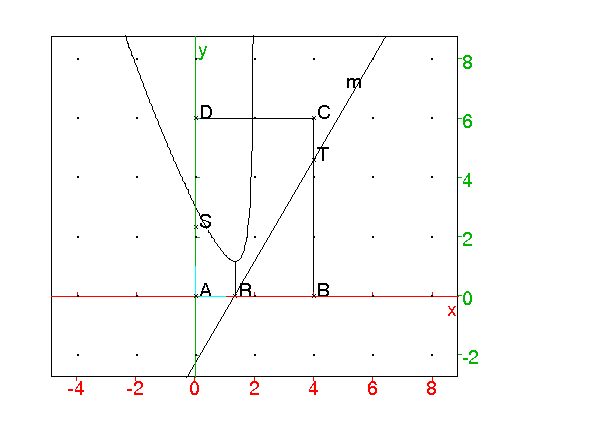
\includegraphics[width=\textwidth]{minia}

\subsection{Les calculs avec {\tt Xcas}}
 On obtient :\\
\begin{itemize}
\item dans le premier cas :\\
{\tt equation(m)} et on obtient {\tt Y=(4/s*X+(s\verb|^|2-16)/(2*s))}\\
{\tt coordonnees(R)} et on obtient {\tt [-1/8*s\verb|^|2+2,0]}\\
{\tt normal(coordonnees(T))} et on obtient {\tt [4,(s\verb|^|2+16)/(2*s)]}\\
{\tt AT:=aire(triangle(R,B,T))} et on obtient {\tt (s\verb|^|2+16)/2/s*(1/8*s\verb|^|2+2)/2}\\
mais toutes les r\'eponses sont fonction de {\tt s} qui a \'et\'e choisi comme 
param\`etre.\\
Si on veut avoir la relation liant $b$ et $a$ on tape :\\
{\tt factor(resultant(a-r[0],numer(b-t[1]),s))} \\
on obtient :\\
{\tt 32*(2*a\verb|^|2+a*b\verb|^|2-16*a-2*b\verb|^|2+32)}
donc {\tt 2*a\verb|^|2+a*b\verb|^|2-16*a-2*b\verb|^|2+32=0}
\item dans le deuxi\`eme cas :\\
pour {\tt equation(m)}, on obtient {\tt y=((-(sqrt(-2*a+4)))/(a-2)*x+a*sqrt(-2*a+4)/(a-2))}\\
pour {\tt coordonnees(S)}, on obtient {\tt [0,sqrt((-a+4)\verb|^|2-a\verb|^|2)]}\\
pour {\tt normal(coordonnees(T))}, on obtient 
{\tt [4,(a-4)*sqrt(-2*a+4)/(a-2)]}\\
pour {\tt AT:=aire(triangle(R,B,T))}, on obtient 
{\tt (a-4)*sqrt(-2*a+4)/(a-2)*(4-a)/2}\\
donc {\tt b=(a-4)*sqrt(-2*a+4)/(a-2)} ou encore :\\
si $a\neq 2$ on a :\\
{\tt factor(b\verb|^|2*(a-2)\verb|^|2-(a-4)\verb|^|2*(4-2*a))=0} 
{\tt (a-2)*(b\verb|^|2*a-2*b\verb|^|2+2*a\verb|^|2-16*a+32)=0}
donc {\tt 2*a\verb|^|2+a*b\verb|^|2-16*a-2*b\verb|^|2+32=0}
\end{itemize}
\subsection{La d\'emonstration}
\subsubsection{Les valeurs minimales et maximales de $a$}
En faisant bouger {\tt s} ou {\tt a}, on voit que {\tt R} va se d\'eplacer du 
point {\tt A}
 au point {\tt R1} d'abscisse {\tt a1} qui correspond \`a {\tt S} en {\tt S1}
et {\tt T} en {\tt C}, c'est \`a dire lorsque {\tt m} passe par {\tt C}.\\ 
On a alors :\\
$S=0+i*s$ avec $0 \leq s \leq 6$ et $SC=6$ donc $S$ est sur le cercle de centre
{\tt C} et de rayon 6 qui a pour \'equation : $(X-4)^2+(Y-6)^2=36$\\
si $X=0$ on a $(Y-6)^2=36-16=20$ donc $s=6-\sqrt{20}=6-2\sqrt 5$\\
On a :\\
$S1R1=4-a1$, $AR1=a1$ et $AS1=6-2\sqrt 5$\\
comme le triangle $AS1R1$ est rectangle en $A$ on a :\\
$(4-a1)^2=a1^2+(6-2\sqrt 5)^2=a1^2+-24*\sqrt 5+56$\\
donc\\
$-8*a1=-24*\sqrt 5+40$\\
donc $a1=3*\sqrt 5-5$.\\
Autre solution :\\
Le triangle $DS1C$ est rectangle donc $DS1^2=36-16=20=(6-s1)^2$ soit 
$DS1=2\sqrt 5$\\
Les triangles rectangles $AR1S1$ et $DS1C$ sont semblables donc :\\
$AR1/DS1=a1/(2\sqrt 5)=R1S1/S1C=(4-a1)/6$ soit\\
$a1(6+2\sqrt 5)=8\sqrt 5$ donc\\
$a1=8\sqrt 5*(6-2\sqrt 5)/16=3\sqrt 5-5$\\
Donc $0 \leq a \leq 3\sqrt 5-5 \simeq 1.7082039325$.\\

\subsubsection{Relation entre $a$ et $b$}
Soit $E$ la projection de $T$ sur $AD$.\\
Le triangle $ARS$ est rectangle en $A$ donc $AS^2=SR^2-AR^2$ soit :\\
$s^2=(4-a)^2-a^2=8*(2-a)$
Les triangles rectangles $ARS$ et $EST$ sont semblables donc :\\
$RS/ST=(4-a)/b=AS/ET=s/4$ soit\\
$s=4(4-a)/b$, soit $s^2=16*(4-a)^2/b^2=8*(2-a)$ donc :\\
$(2-a)*b^2-2*(4-a)^2=0$\\
Si on d\'eveloppe :\\
{\tt expand((2-a)*b\verb|^|2-2*(4-a)\verb|^|2)}, on trouve
{\tt -b\verb|^|2*a+2*b\verb|^|2-2*a\verb|^|2+16*a-32}
\subsubsection{Valeur de $a$ pour que l'aire de $BRT$ soit minimale}
On veut avoir $(4-a)*b$ minimum. On pose $u=(4-a)*b$ on a donc :\\
$b=u/(4-a)$ donc $=0$ soit \\
$(2-a)*u^2=2*(4-a)^4$ c'est \`a dire :\\
$u^2=2*(4-a)^4/(2-a)$\\
On cherche les variations de $u$ et on tape :\\
{\tt factor(diff(2*(4-a)\verb|^|4/(2-a),a))}\\
On obtient :\\
{\tt (-2*(3*a-4)*(a-4)\verb|^|3)/((a-2)\verb|^|2)}
{\tt u*u'} est positif  pour {\tt a>4/3} et est negatif pour {\tt a<4/3}.\\
Donc lorsque {\tt a=4/3}, {\tt u} est minimum. \\
On tape :\\ 
{\tt subst(2*(4-a)\verb|^|4/(2-a),a=4/3)}\\
On obtient :\\
{\tt 4096/27}
Donc la surface minimum vaut :\\
{\tt normal(sqrt(4096/27))=(192*sqrt(3))/27} \\
la valeur de {\tt b} est :\\
{\tt normal((192*sqrt(3))/27/(4-4/3))=8*sqrt(3)/3}
a valeur de {\tt s} est :\\
{\tt normal(sqrt(8*(2-4/3)))=(4*sqrt(3))/3}\\
Dans ce cas le triangle $BTR$ est un demi triangle \'equilat\'eral puisque :\\
{\tt b=8*sqrt(3)/3} et {\tt 4-a=8/3}.\\
L'angle {\tt T} du triangle isoc\`ele $BTS$ vaut donc $pi/3$ : ce triangle est 
donc \'equilat\'eral. 
\section{La boite de biscuits}
\subsection{L'\'enonc\'e 1}
On veut emballer 40 biscuits d'epaisseur 0.5 $cm$ et ayant la forme d'un quart 
de cercle de rayon 5 $cm$ dans une boite ayant la forme d'un 
parall\'el\'epip\`ede rectangle. Les biscuits sont dans 2 sachets fraicheur de 
20 biscuits et ayant chacun 10 $cm$ de haut.
\begin{itemize}
\item On d\'ecide  de mettre les 2 
sachets bout \`a bout. Quelle sont les dimensions de la boite et calculer sa surface.
\item On d\'ecide de mettre les 2 sachets de fa\c{c}on qu'ils soient tangents.
Quelle sont les dimensions de la boite et calculer sa surface.
\item Quelle est la boite la plus \'economique ?
\end{itemize}
\subsection{Solution de l'\'enonc\'e 1}
La r\'eponse :
\begin{itemize}
\item La boite a comme dimension : $20\times 5\times 5$. Sa surface est donc:
2*5*5+20*4*5=450 $cm^2$.
\item On ouvre un \'ecran de g\'eom\'etrie ({\tt Alt+g}) et on tape :
{\tt cercle(point(0),5,0,pi/2,affichage=1+rempli)}
cela dessine le premier biscuit. La position du deuxi\`eme biscuit aura  pour 
centre {\tt point(a,5)} et il faut trouver {\tt a} pour que les 2  
cercles soient tangents.\\
On tape :
\begin{verbatim}
 cercle(point(0),5,0,pi/2,affichage=1+rempli);
supposons(a=[8.66,5,10,0.01]);
 cercle(point(a,5),5,pi,3*pi/2,affichage=3+rempli);
I:=inter(cercle(point(a,5),5,pi,3*pi/2),
cercle(point(0),5,0,pi/2))
\end{verbatim}
et on fait bouger le curseur {\tt a}. On trouve que 
{\tt a} est proche de 8.66 car il n'y a qu'un point d'intersection.\\
Pour faire un calcul exact \`a la main, il suffit de savoir que le point de 
tangence des deux biscuits se trouve au milieu du segment qui joint les centres
 qui est ici le {\tt segment(0,point(a+5*i))}. Lorsque les 2 cercles sont 
tangents ce segment a pour longueur 10 $cm$. Donc on a d'apr\`es le 
th\'eor\`eme de Pythagore :\\
$a^2=10^2-5^2=75$ donc $a=5\sqrt 3 \simeq 8.66025403784$.\\
La boite a comme dimension : $10\times 5\times 5\sqrt 3$. Sa surface est donc:
$2*5*5\sqrt 3+10*2*(5+ 5\sqrt 3)=100+150\sqrt 3=359.807621135\ cm^2$
\item La deuxi\`eme boite de suface $359.807621135\ cm^2$ est la plus 
\'economique.
\end{itemize}
On a :\\
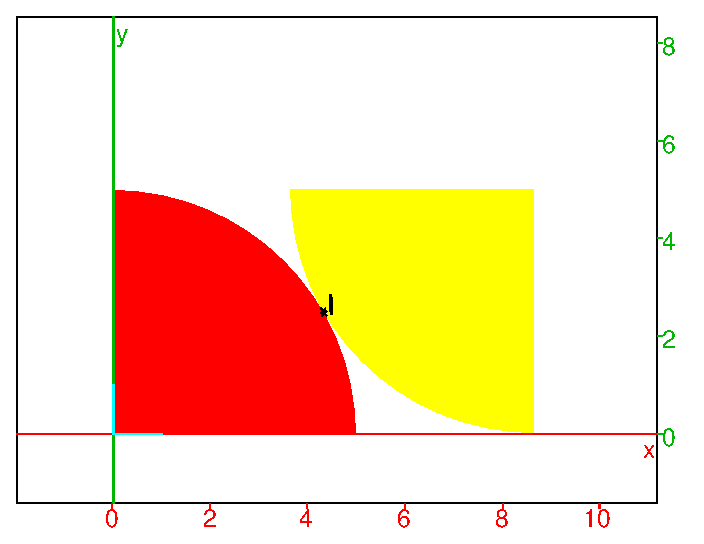
\includegraphics[width=\textwidth]{biscuit2}

\subsection{L'\'enonc\'e 2}
On veut emballer 40 biscuits d'epaisseur 0.5 $cm$ et ayant la forme d'un quart 
de cercle de rayon 5 $cm$ dans une boite ayant la forme d'un 
parall\'el\'epip\`ede rectangle. Les biscuits sont dans 5 sachets fraicheur de 
8 biscuits et ayant chacun 4 $cm$ de haut.\\
 On d\'ecide de mettre un sachet dans chaque coin de la boite et 1 sachet 
au milieu, de fa\c{c}on qu'ils soient tangents aux 4 autres.
Quelle est la dimension de la boite de surface minimum ?
\subsection{Solution de l'\'enonc\'e 2}
La r\'eponse :\\
On ouvre un \'ecran de g\'eom\'etrie ({\tt Alt+g}).
Le premier biscuit sera {\tt cercle(point(0),5,0,pi/2,affichage=1+rempli)}. \\
On choisit un param\`etre {\tt a} et on positionne le deuxi\`eme biscuit dans 
le coin  {\tt D:=point(0,10+2*a)}\\
Le cinqui\`eme biscuit (celui que l'on met au milieu de la boite) aura pour 
centre $I$ qui sera le point d'intersection de la tangente au biscuit 1 
d'\'equation $y=-x+5*\sqrt 2$ avec $y=5+a$.\\
Le troisi\`eme biscuit doit \^etre tangents au cinqui\`eme biscuit, son 
centre $J$ est donc sur l'axe des $x$ et sur le cercle de centre $I$ et de 
rayon 10. IL faut bien s\^ur imposer que {\tt abscisse(J)>=10}
Il faut trouver {\tt a} pour que la surface de la boite soient minimum.\\
On tape :
\begin{verbatim} 
cercle(point(0),5,0,pi/2,affichage=1+rempli);
supposons(a=[1.66,0,5,0.01]);
cercle(point(0,10+2*a),5,3*pi/2,2*pi,affichage=2+rempli);
I:=inter_unique(droite(y=5+a),droite(y=-x+5*sqrt(2)));
cercle(I,5,-pi/4,pi/4,affichage=5+rempli);
J:=inter(droite(y=0),cercle(I,10))[0]:;
cercle(J,5,pi/2,pi,affichage=3+rempli);
cercle(translation((10+2*a)*i,J),4,pi,3*pi/2,affichage=5+rempli);
xj:=normal(abscisse(J))
evalf(xj*(10+2*a)*2+2*4*(xj+10+2*a)
\end{verbatim}
et on fait bouger le curseur {\tt a}. 
On trouve que {\tt a} varie entre 0 et 0.453289254261.\\
En effet :
{\tt xj:=normal(abscisse(J))} renvoie :\\
{\tt -a+5*sqrt(2)-5+sqrt(-a\verb|^|2-10*a+75)} et\\ 
{\tt evalf(solve(-a\verb|^|2-10*a+75-(15+a-5*sqrt(2))\verb|^|2=0,a))}\\
renvoie {\tt [-13.3822214424,0.453289254261]}\\
la surface de la boite est donc :\\
{\tt  xj*(10+2*a)*2+8*(xj+10+2*a)}\\
qui varie de {\tt 380.477011792} \`a {\tt 385.361761927} lorsque {\tt a} varie 
de {\tt 0} \`a  {\tt 0.45}\\
Donc on prend {\tt a=0} et alors {\tt xj} vaut {\tt 5*sqrt(2)-5+5sqrt(3)} ou
 encore {\tt 10.7313218497}\\
La boite est donc de dimensions $4*5*(5\sqrt 2-5+5\sqrt 3)$ et sa surface vaut
{\tt 20*(5*sqrt(2)-5+5*sqrt(3))+8*(5*sqrt(2)-5+5*sqrt(3)+80)} c'est\`a dire :\\
{\tt 28*(5*sqrt(2)-5+5*sqrt(3))+80} ou encore {\tt 380.477011792}\\
On obtient :\\
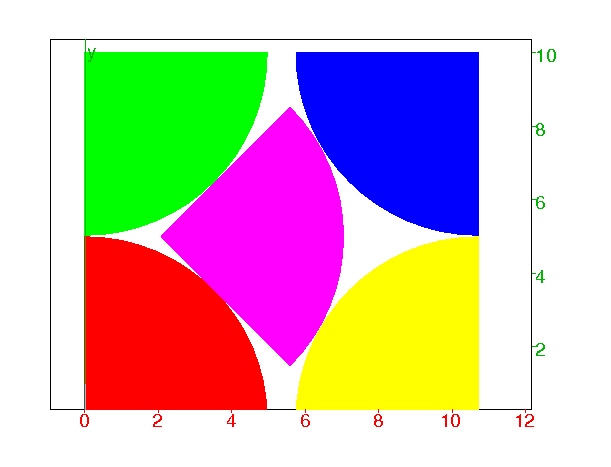
\includegraphics[width=\textwidth]{biscuit5}
\section{Une construction g\'eom\'etrique : inscrire un carr\'e dans une "goutte"}
\subsection{L'\'enonc\'e}
Une goutte d'eau represent\'ee ci-dessous est constitu\'ee par 2 demi-cercles 
$C2$ et $C3$ de centre $O2$ et $O3$ et rayon $r$ et d'un demi-cercle $C1$ de 
centre $O$ et de rayon $2r$.\\ 
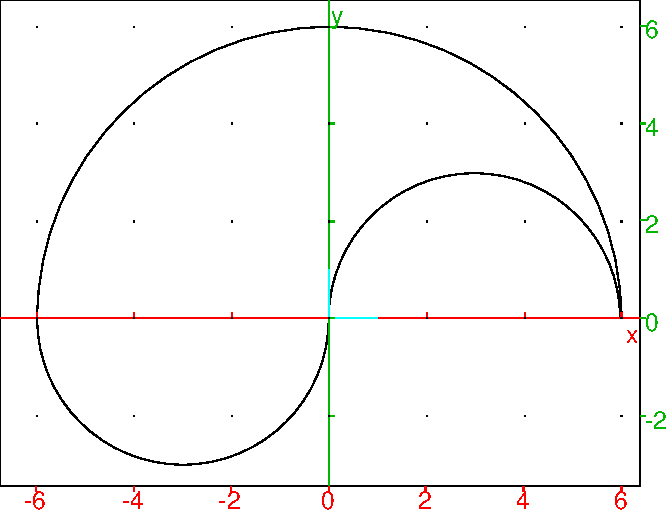
\includegraphics[width=\textwidth]{goutte}\\
On cherche \`a placer 4 $A,B,C,D$ points surle contour de cette goutte pour que
$ABCD$ soit un carr\'e.\\
Pour chercher, on fait la figure suivante et on tape dans un \'ecran de 
g\'eom\'etrie :
\begin{verbatim}
C1:=cercle(0,6,0,pi):;C1;
C2:=cercle(3,3,0,pi):;C2;
C3:=cercle(-3,3,pi,2*pi):;C3;
a:=element(0 .. pi,1.947787474,0.031415927);
A:=element(C1,a);
c:=element(pi .. (2*pi),4.618141269,0.031415927)
C:=element(C3,c);
C4:=cercle(A,C,affichage=rouge);
B:=inter(C4,C1)[0];
D:=inter(C4,C2)[1];
polygone(A,B,C,D);
O:=point(0);
\end{verbatim}
On fait bouger les curseurs {\tt a} et {\tt c} pour essayer d'avoir un 
rectangle et on obtient :
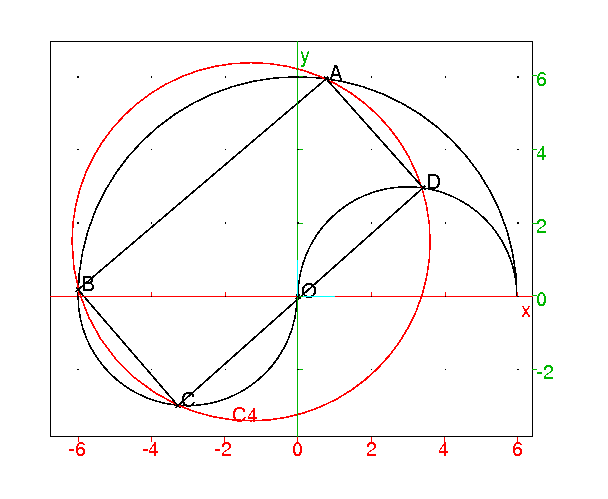
\includegraphics[width=\textwidth]{goutter}\\
Il semble que le segment $CD$ passe par $O$.\\
\subsection{Des  lemmes sur les rectangles et leur cercle circonscrit}
Les lemmes qui suivent vont montrer que si un rectangle direct $ABCD$ a ses 
sommets sur le pourtour de la goutte un de ses sommets est le point 
d'intersection $A$ de $C1$ et $C3$ et son c\^ot\'e $CD$ passe par $0$.\\

{\bf Lemme 1}\\
Si 3 sommets d'un rectangle sont sur un demi-cercle $\Gamma$ de centre $O$, 
alors le quatri\`eme sommet se trouve sur le demi-cercle $\gamma$ sym\'etrique 
de $\Gamma$ par rapport \`a $O$. Dans le cas de la goutte cela veut 
dire que si un rectangle a ses sommets sur le pourtour de la goutte, il ne peut
pas y avoir 3 sommets sur le m\^eme demi cercle.\\ 

{\bf Lemme 2}\\
Si 2 sommets $M$ et $P$ d'un rectangle sont sur un demi-cercle $\Gamma$ de 
centre $O$, alors ces sommets sont cons\'ecutifs car sinon le centre de 
$\Gamma$ serait le milieu de $MP$ et le rectangle aura ses 4 sommets  sur le 
cercle de diam\`etre $MP$ (cercle qui contient $\Gamma$). Dans le cas de la 
goutte cela veut dire que si un rectangle a deux sommets sur un m\^eme 
demi-cercle (faisant partie du pourtour de la goutte) alors ces 2 sommets sont 
cons\'ecutifs.\\ 

{\bf Lemme 3}\\
Soient $c1$, $c2$ et $c3$ les cercles compl\'etant $C1$, $C2$ et $C3$
Montrons qu'il n'y a pas de rectangle ayant tous ses sommets sur $C2\cup C3$.
En effet, si par exemple $A$ et $B$ sont sur $C3$ et si $C$ et $D$ sont sur 
$C2$ : l'angle $A$ est droit donc le sym\'etrique $B1$ de $B$ par rapport \`a 
$O3$ se trouve sur $AD$ et sur $c3$ et l'angle $B$ est droit donc le 
sym\'etrique $A1$ de $A$ par rapport \`a $O3$ se trouve sur $BC$ et sur $c3$ : 
les deux droites $AD$ et $BC$ sont donc sym\'etriques par rapport \`a $O3$.\\
De m\^eme l'angle $C$ est droit donc le sym\'etrique $D1$ de $D$ par rapport 
\`a $O2$ e trouve sur $BC$ et sur $c2$ etc...Donc les deux droites $AD$ et $BC$
sont donc sym\'etriques par rapport \`a $O2$.\\
Donc $AD$ et $BC$ sont parall\'eles \`a $O2O3$ c'est \`a dire que $AB$ et $AC$ sont confondus et le rectangle se r\'eduit \`a une droite.\\

{\bf Lemme 4}\\
Supposons  qu'il y ait 2 sommets $A$ et $B$ sur le demi-cercle $C2$. Les 
c\^ot\'es $AD$ et $BC$ sont sym\'etriques par rapport \`a $O2$ et ces 
c\^ot\'es coupent $C1$ et $C3$ en des points qui sont de part et d'autre de 
$AB$. Donc $A$ et $B$ ne sont pas cons\'ecutifs.\\

{\bf Lemme 5}\\
Supposons  qu'il y ait 2 sommets $A$ et $B$ sur le demi-cercle $C3$. Les 
c\^ot\'es $AD$ et $BC$ sont sym\'etriques par rapport \`a $O3$.\\
Supposons que $D$ soit sur $C1$ et que $AD$ coupe $c1$ en 
$D1$. L'angle $D$ est droit donc $DC$ passe par $D2$ sym\'etrique de $D1$ par 
rapport \`a $O$ et donc $D2$ est sur $C1$.\\
$BC$ coupe le cercle $c3$ en $A3$ sym\'etrique de $A$ par rapport \`a $O3$ et 
coupe le cercle $C2$ en $A2$ et en $C$. L'angle $C$ est droit donc $DC$ passe 
par $A3$ sym\'etrique de $A2$ par rapport \`a $O2$ et donc $A3$ est sur $c2$.\\
Donc si $DC$ passe par $D2$ situ\'e sur $C1$, il ne peut pas couper $c2$ que si $D2$ et $A3$ sont confondus et sont sur la droitre $OO2$ c'est \`a dire si $A$ 
se trouve en $P$ intersection de $C1$ et $C3$.\\
M\^eme raisonnement si $C$ est sur $C1$ et $D$ sur $C2$.  

{\bf Lemme 6}\\
Il y a 2 sommets sur le demi-cercle $C$ 
Soient $da$ et $db$ les perpendiculaires \`a $AB$ en $A$ et $B$. Consid\'erons 
$A1$ et $B1$ les sym\'etriques de $A$ et $B$ par rapport \`a $O$. Puisque $AA1$
et $BB1$ sont des diam\`etres du cercle  de centre $O$ et de rayon $2r$,  $da$
 passe par $B1$ et $db$ passe par $A1$. $AB1$ et $A1B$ sont des segments 
sym\'etriques par rapport \`a $O$ et les demi-cercles de rayon $r$ sont aussi 
sym\'etriques par rapport \`a $O$. Donc $AB1$ et $A1B$ coupent les demi-cercles de rayon $r$ en deux points  $D$ et $C$  sym\'etriques par rapport \`a $O$.
Donc $DC$ passe par $O$.
\subsection{Construction du carr\'e}
Si $A$ et $B$ sont sur le demi-cercle de centre $O$ et de rayon $2r$ alors le 
segment $CD$ passe par $O$ si les angles $A$ et $B$ de $ABCD$ sont droits,
On tape :
\begin{verbatim}
C1:=cercle(0,6,0,pi):;C1;
C2:=cercle(3,3,0,pi):;C2;
C3:=cercle(-3,3,pi,2*pi):;C3;
O:=point(0);
a:=element(0 .. pi,1.947787474,0.031415927);
A:=element(C1,a);
b:=element(0 .. pi,2.82743343,0.031415927;)
B:=element(C1,b);
C5:=cercle(0,6,pi,2*pi):;affichage(C5,1);
A1:=symetrie(O,A);
B1:=symetrie(O,B);
s1:=segment(A,B1):;s1;
s2:=segment(A1,B):;s2;
D:=inter(C2,s1)[1];
C:=inter(C3,s2)[1];
segment(A,B);
\end{verbatim}
On obtient :\\
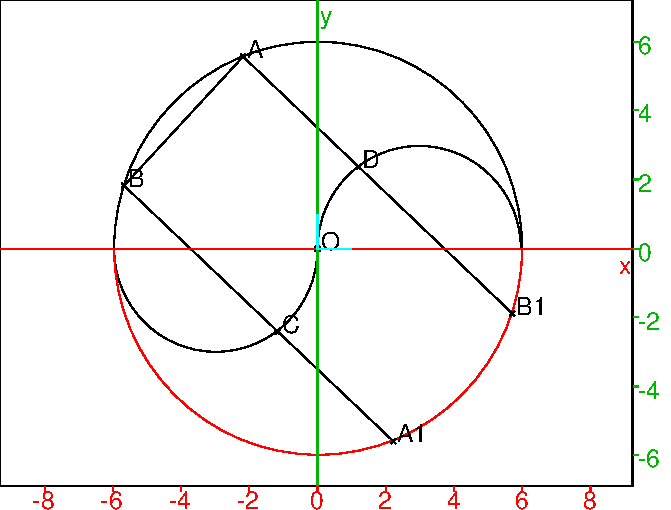
\includegraphics[width=\textwidth]{goutted}

Pour avoir un carr\'e il suffira de choisir $OA=2r$ et $OD=AD/2$ donc
$OD^2+AD^2=5*OD^2=4*r^2$ c'est \`a dire :\\
$OD=2r\sqrt5/5$.\\
Dans la figure on a choisit $r=3$ donc $OD=6/5*sqrt5$ $OD$ est donc 
l'hypot\'enuse d'un triangle rectangle de c\^ot\'e 6/5 et 12/5.
Si le point {\tt D1:=point(12/5,6/5):;D1}, on a $OD=OD1$.\\
On tape dans un \'ecran de g\'eom\'etrie :
\begin{verbatim}
C1:=cercle(0,6,0,pi):;C1;
C2:=cercle(3,3,0,pi):;C2;
C3:=cercle(-3,3,pi,2*pi):;C3;
O:=point(0);
D1:=point(12/5,6/5):;D1;
D:=inter(C2,cercle(O,longueur(O,D1)))[0];
C:=symetrie(O,D);
carre(C,D,A,B);
\end{verbatim}
On obtient :
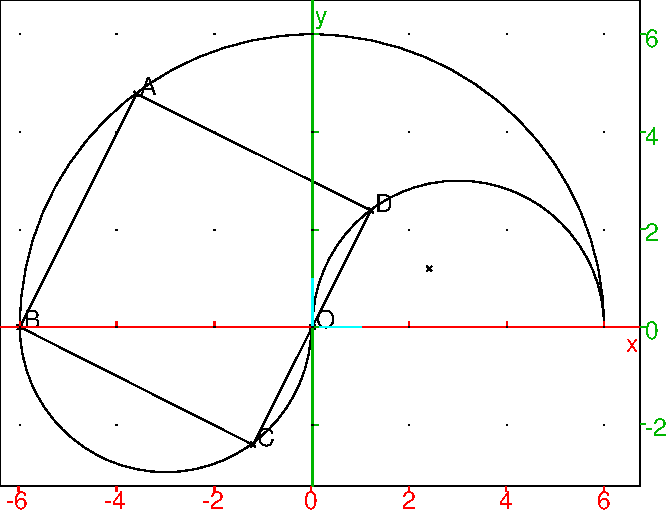
\includegraphics[width=\textwidth]{gouttec}\\
On remarque que :\\
le point $B$ est sur l'axe des $x$ car l'angle $C$ est droit,\\
le point $D$ a pour coordonn\'ees $6/5,12/5$.

\chapter{G\'eom\'etrie dans l'espace seconde et terminale}
\subsection{Exercice 1}
Soit $ABCDE$ une pyramide de sommet $E$ et de base rectangulaire $ABCD$.
On sait que $AE=21$, $BE=36$ et $CE=18$.\\
Calculer  $DE$ \\
Trouver une formule g\'en\'erale reliant $AE,BE,CE,DE$.\\
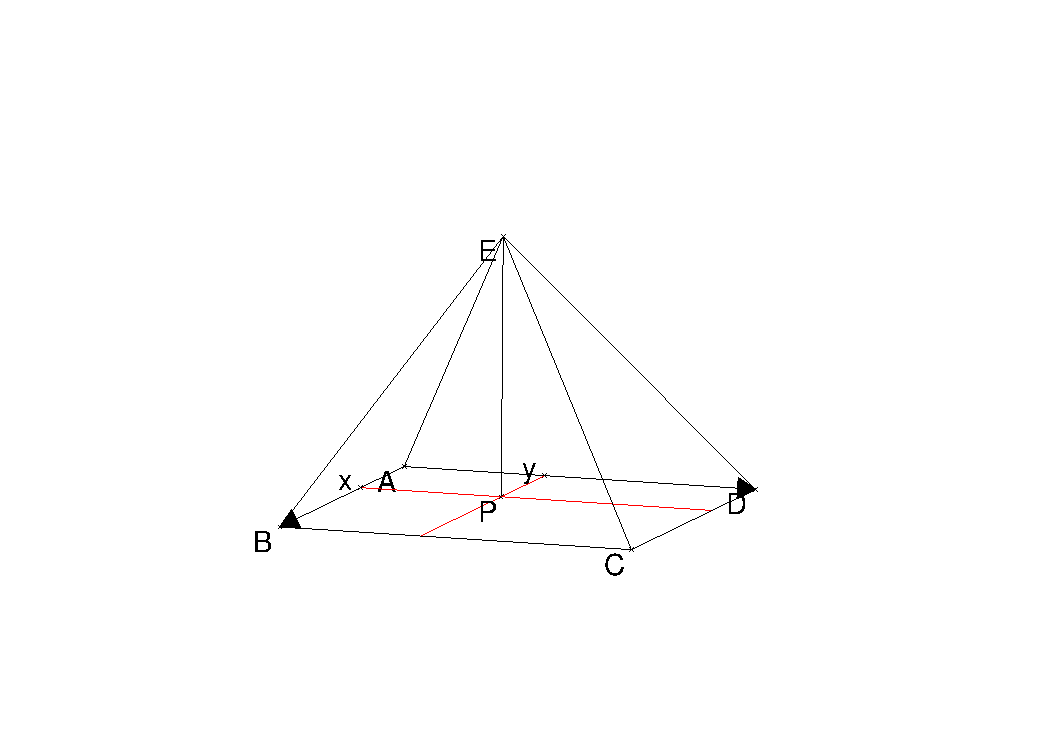
\includegraphics[width=\textwidth]{pyramide}\\

Soient $P$ la projection de $E$ sur le plan $ABCD$ et $x$ et $y$ les coordonn\'ees de $P$ dans le rep\`ere $(A,\overrightarrow{AB},\overrightarrow{AC})$.\\
On a :\\
$AP^2=x^2+y^2$\\
$BP^2=(AB-x)^2+y^2$\\
$CP^2=(AB-x)^2+(AD-y)^2$\\
$DP^2=x^2+(AD-y)^2$\\
Donc :\\
$AE^2=AP^2+PE^2=x^2+y^2+PE^2$
$BE^2=(AB-x)^2+y^2+PE^2$\\
$CE^2=(AB-x)^2+(AD-y)^2+PE^2$\\
$DE^2=x^2+(AD-y)^2+PE^2$\\
On en d\'eduit que :\\
$AE^2-BE^2+CE^2=x^2+(AD-y)^2+PE^2=DE^2$\\
D'o\`u la formule :
$$AE^2+CE^2=BE^2+DE^2$$
{\bf Application num\'erique}
Si $AE=21$, $BE=36$ et $CE=18$, on a :\\
$DE=21^2+18^2-36^2$\\
On tape :\\
{\tt sqrt(21\verb|^|2+18\verb|^|2-36\verb|^|2)}\\
On obtient :\\
{\tt 27}
\subsection{Exercice 2}
\chapter{Le "baccalaur\'eat" suisse de 1896}
Il s'agit des \'epreuves que Einstein passe en 1896 \`a l'age de 17 ans et demi
en Suisse, ce qui est l'\'equivalent de notre  baccalaur\'eat.\\ 
\`A l'\'epoque tous les calculs \'etaient lons et fastidieux car faits \`a 
l'aide de table\section{\'Epreuve de g\'eom\'etrie de 4h}
\subsection{Exercice 1}
\subsubsection{L'\'enonc\'e}
Un triangle inscrit dans un cercle de rayon $R=10$ a ses hauteurs 
proportionnelles \`a 2, 3 et 4.\\
Calculer les angles et un c\^ot\'e.
\subsubsection{La solution avec {\tt Xcas}}
Par hypoth\`ese, il existe $k\in \R^+$ tel que :\\
$h_A=2k$, $h_B=3k$, $h_C=4k$,\\
On a :\\
$\displaystyle \sin(A)=\frac{h_B}{c}=\frac{h_C}{b}=\frac{3k}{c}=\frac{4k}{b}$\\
$\displaystyle \sin(B)=\frac{h_A}{c}=\frac{h_C}{a}=\frac{2k}{c}=\frac{4k}{a}$\\
$\displaystyle \sin(C)=\frac{h_B}{a}=\frac{h_A}{b}=\frac{3k}{a}=\frac{2k}{b}$\\
Donc :\\
$a=2c$ et $b=\frac{4c}{3}$ et\\
$a^2=c^2+b^2-2bc\cos(A)$ \\
$b^2=a^2+c^2-2ac\cos(B)$ \\
$c^2=a^2+b^2-2ab\cos(C)$ \\
On fait une figure  :\\
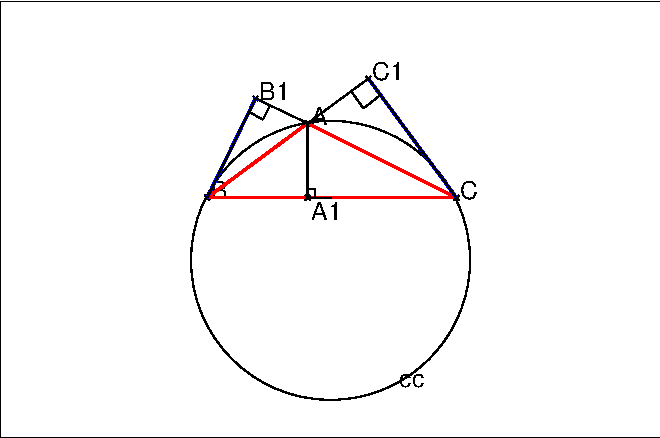
\includegraphics[width=\textwidth]{baceinst0}\\
Donc on a:
\begin{itemize}
\item $\displaystyle 4c\frac{4c}{3}\cos(C)=c^2(4+\frac{16}{9}-1=c^2\frac{43}{9}$soit :\\
$\displaystyle \cos(C)=\frac{43}{16*3}=\frac{43}{48}\ $ et 
$\displaystyle\ \sin(C)=\frac{\sqrt{455}}{48}$\\
On tape :\\
{\tt C:=acos(43/48.)}\\
On obtient :\\
{\tt 0.460493425059}\\
\item 
$\displaystyle 4c^2\cos(B)=4c^2+c^2-\frac{16c^2}{9}=c^2\frac{29}{9}$ soit : \\
$\displaystyle \cos(B)=\frac{29}{36}\ $
et 
$\displaystyle\ \sin(B)=\frac{\sqrt{455}}{36}$\\
On tape :\\
{\tt B:=acos(29/36.)}\\
On obtient :\\
{\tt 0.634183840824}\\
\item 
$\displaystyle 2c\frac{4c}{3}\cos(A)=+c^2+\frac{16c^2}{9}-4c^2=c^2\frac{-11}{9}$soit : \\
$\displaystyle \cos(A)=\frac{-11}{24}\ $ et 
$\displaystyle \ \sin(A)=\frac{\sqrt{455}}{24}$\\
On tape :\\
{\tt A:=acos(-11/24.)}\\
On obtient :\\
{\tt 2.04691538771}\\
\end{itemize}
On sait que :\\
$\displaystyle \frac{a}{\sin(A)}=\frac{b}{\sin(B)}=\frac{c}{\sin(C)}=2R=20$ et \\
Donc on a :\\
\begin{itemize}
\item $\displaystyle c=20\sin(C)=\frac{5\sqrt{455}}{12}$\\
On tape :\\
{\tt c:=5*sqrt(455)/12.)}\\
On obtient :\\
{\tt 8.88780375321}\\
\item $\displaystyle b=\frac{4c}{3}=\frac{5\sqrt{455}}{9}$\\
On tape :\\
{\tt b:=4c/3}\\
On obtient :\\
{\tt 11.8504050043}\\
\item $\displaystyle a=2c=\frac{5\sqrt{455}}{6}$\\
On tape :\\
{\tt a:=2*c)}\\
On obtient :\\
{\tt 17.7756075064}\\
\end{itemize}
On construit le triangle $ABC$ et on tape :
\begin{verbatim}
B:=point(0);
C:=point(5*sqrt(455)/6);
A:=point(5*sqrt(455)/12*(29/36+i*sqrt(455)/36));
triangle(A,B,C);
cc:=circonscrit(A,B,C);
\end{verbatim}
%On obtient :\\
%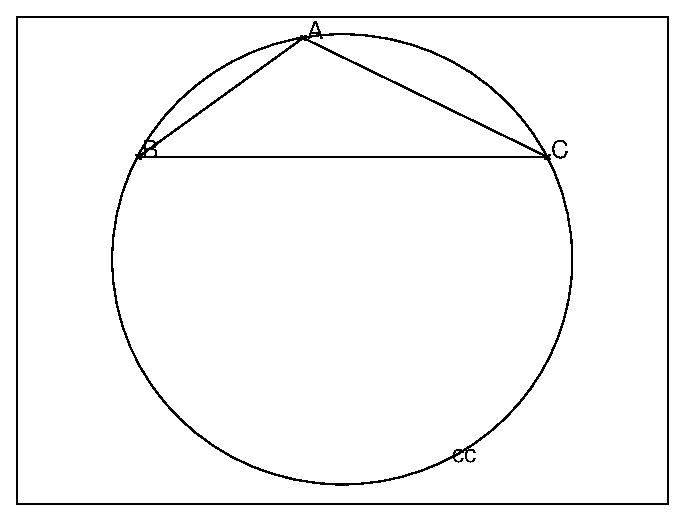
\includegraphics[width=\textwidth]{baceinst1}\\
0n tape :\\ 
{\tt normal(rayon(cc));}\\
On obtient : {\tt 10}\\
0n tape :\\ 
{\tt A1:=projection(droite(B,C),A);}\\
{\tt normal(longueur(A,A1));}\\
On obtient : {\tt 2275/432}\\
Donc le coefficient de proportionnalit\'e $k$ pour les hauteurs vaut : \\
$\displaystyle \frac{2275}{864}$
\subsubsection{Une autre solution avec {\tt Xcas}}
Si $S$ est l'aire du triangle $ABC$ on a :\\
$2S=ah_A=bh_B=ch_c$\\
Par hypoth\`ese, il existe $k\in \R^+$ tel que :\\
$h_A=2k$, $h_B=3k$, $h_C=4k$ donc,\\
$2a=3b=4c$ c'est\`a dire $a=2c$ et $b=4/3c$\\
Le triangle $ABC$ est donc semblable au triangle de c\^ot\'es :\\
$a=6, b=4, c=3$\\
On sait que le rayon $R$ du cercle circonscrit est \'egal \`a :\\
$\displaystyle R=\frac{abc}{4\sqrt{p(p-a)(p-b)(p-c)}}$ avec $2p=a+b+c$.\\
 Avec {\tt Xcas}, on calcul le rayon du cercle circonscrit au triangle 
$a=6, b=4, c=3$, on tape :\\
{\tt a:=6}\\
{\tt b:=4}\\
{\tt c:=3}\\
{\tt p:=(a+b+c)/2}\\
{\tt R:=a*b*c/4/sqrt(p*(p-a)*(p-b)*(p-c))}\\
On obtient : \\
{\tt (72*sqrt(455))/455}\\
On veut avoir que le rayon du cercle circonscrit soit \`egale \`a 10 donc le 
triangle cherch\'e est proportionnel au triangle de c\^ot\'es 
$a=6, b=4, c=3$ avec comme coefficient de proportionnalit\'e :\\
$k= \frac{10\sqrt{455}}{72}=\frac{5\sqrt{455}}{36}$.\\
Les c\^ot\'es du triangle cherch\'e sont donc :\\
$BC=\displaystyle \frac{5 \sqrt{455}}{6},\ $
$\ AC=\displaystyle\ \frac{5 \sqrt{455}}{9},\ $
$\ AB=\displaystyle\ \frac{5 \sqrt{455}}{12}\ $\\
Les angles de $ABC$ sont les m\^emes que les angles du triangle de c\^ot\'es 
$a=6, b=4, c=3$ donc on a :\\
$2bc\cos(A)=b^2+c^2-a^2$ \\
$2ac\cos(B)=a^2+c^2-b^2$ \\
$2ab\cos(C)=a^2+b^2-c^2$ \\
 Avec {\tt Xcas}, on tape :\\
{\tt A:=evalf(acos((b\verb|^|2+c\verb|^|2-a\verb|^|2)/(2*b*c)))}\\
On obtient : \\
{\tt 2.04691538771}\\
On tape :\\
{\tt B:=evalf(acos((a\verb|^|2+c\verb|^|2-b\verb|^|2)/(2*a*c)))}\\
On obtient : \\
{\tt 0.634183840824}\\
On tape :\\
{\tt C:=evalf(acos((a\verb|^|2+b\verb|^|2-c\verb|^|2)/(2*a*b)))}\\
On obtient : \\
{\tt 0.460493425059}
\subsubsection{La solution de {\tt Xcas}}
{\tt Xcas} fait de la g\'eom\'etrie analytique.\\
On dessine le triangle direct $ABC$ de c\^ot\'es $a=6, b=4, c=3$ en mettant 
$B$ \`a l'origine du rep\`ere et $C$ sur l'axe des $x$.\\
On tape :
\begin{verbatim}
B:=point(0);
C:=point(6);
A:=inter(cercle(0,3),cercle(5,4))[1];
triangle(A,B,C,affichage=1+epaisseur_ligne_2);
tA:=angle(A,B,C);
tB:=angle(B,C,A);
tC:=angle(C,A,B);
cc:=circonscrit(A,B,C);
R:=rayon(cc);
\end{verbatim}
On obtient :\\
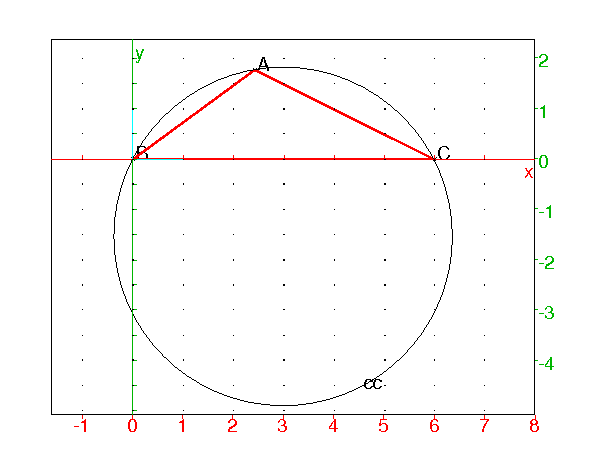
\includegraphics[width=\textwidth]{baceinst3}\\
Avec :\\
pour {\tt tA : atan(((sqrt(455))/2)/(-11/2))+(2*pi)/2}\\
pour {\tt tB :atan(((sqrt(455))/2)/(29/2))}\\
pour {\tt tC : -(atan(((sqrt(455))/2)/(43/2)))}\\
pour {\tt evalf(tA) : 2.04691538771}\\
pour {\tt evalf(tB) : 0.634183840824}\\
pour {\tt evalf(tC) : 0.460493425059}\\
pour {\tt R : (72*sqrt(455))/455}

\subsection{Exercice 2}
\subsubsection{L'\'enonc\'e}
On donne un cercle de rayon $r$ dont le centre se trouve \`a l'origine $O$ d'un
rep\`ere orthonormal.\\
On consid\`ere les cordes de ce cercle perpendiculaires \`a l'axe des $x$.\\
Les cercles ayant  ces cordes comme diam\`etres sont 
tangents \`a l'ellipse de demi-axes $r\sqrt 2$ et $r$, aussi longtemps que la 
distance $d$ de leur centre \`a $O$ ne d\'epasse pas une certaine valeur 
maximale.\\
D\'emontrer cette proposition et d\'eterminer la valeur maximale de $d$.
\subsubsection{La solution avec {\tt Xcas}}
On consid\`ere la corde du cercle centre $O$ et de rayon $r$ qui a pour 
abscisse $-r\leq a\leq r$ et qui est perpendiculaire \`a l'axe des $x$.\\
Le cercle de diam\`etre cette corde a donc pour rayon 
$\sqrt{r^2-a^2}$ et pour \'equation :\\
$(x-a)^2+y^2=r^2-a^2$ ou encore :\\
$x^2+y^2-2ax+2a^2-r^2=0$
Avec {\tt Xcas}, on suppose que $r=1$ et on tape :
\begin{verbatim}
ellipse(-1,1,sqrt(2),affichage 
=1)supposons(a=[0.5,-1/sqrt(2),1/sqrt(2),0.1]);
C:=cerle(a,sqrt(1-a^2));
\end{verbatim}
Puis, on fait bouger $a$ en gardant la trace de {\tt C} (menu {\tt M->Trace objet->C}).\\
On obtient :\\
\includegraphics[width=\textwidth]{baceinst2}\\
Nous allons montrer que l'enveloppe de ces cercles est une ellipse de centre 
$O$ et de demi-axes $r\sqrt 2$ et $r$ (c'est ce que l'on voit sur la figure 
ci-dessus).\\
Le point $M=(x,y)$ de contact  du 
cercle et de son enveloppe v\'erifie les  \'equations :\\
$x^2+y^2-2ax+2a^2-r^2=0$ et\\
$-2x+4a=0$ (obtenu en d\'erivant par rapport \`a $a$)\\ 
donc $M=(2a,\sqrt{r^2-2*a^2})$ ou $M=(2a,-\sqrt{r^2-2*a^2})$.\\
Il faut donc que $r^2-2*a^2\geq 0$ soit $a\leq \frac{r\sqrt 2}{2}$.\\
Puisque  $a=x/2$ $M$ est sur la courbe d'\'equation  :\\
$x^2+y^2-2(x/2)x+2{(x/2)}^2-r^2=x^2+y^2-x^2+x^2/2-r^2=x^2+2y^2-2r^20$.\\
Donc $M$ se d\'eplace donc sur l'ellipse d'\'equation :\\
$x^2+2y^2=2r^2$. \\
Cette ellipse a pour centre $O$ et pour demi-axes $r\sqrt 2$ et $r$.



\section{\'Epreuve d'alg\'ebre de 2h}
\subsection{L'\'enonc\'e}
Dans un triangle on connait les distance $l,\ m,\ n$ du centre du cercle 
inscrit aux sommets.\\
D\'eterminer le rayon $r$ du cercle inscrit lorsque $l=1,\ m=1/2,\ n=1/3$\\ 
\subsubsection{La solution avec {\tt Xcas}}
Soient le triangle $ABC$ et $I$ le centre  de son cercle inscrit.\\
On pose $IA=l$, $IB=m$ et $IC=n$.\\
\includegraphics[width=\textwidth]{baceinst4}\\
On a :\\
$\displaystyle \sin(\frac{A}{2})=\frac{r}{l}=r$, \hspace*{0.3cm}
$\displaystyle \sin(\frac{B}{2})=\frac{r}{m}=2r$, \hspace*{0.3cm}
$\displaystyle \sin(\frac{C}{2})=\frac{r}{n}=3r$\\
On sait que $\widehat A +\widehat B +\widehat C =\pi$ donc\\
$\displaystyle \sin(\frac{C}{2})=\sin(\frac{\pi}{2}-\frac{A+B}{2})=\cos(\frac{A+B}{2})$.\\
On sait que :\\
$\widehat A /2<\pi/2$ donc $\cos(A/2)=\sqrt{1-r^2}$\\
$\widehat B /2<\pi/2$ donc $\cos(B/2)=\sqrt{1-4r^2}$\\
Donc :\\
$\sin(C/2)=\sqrt{1-r^2}\sqrt{1-4r^2}-2r^2=3r$
$r$ v\'erifie donc l'\'equation :\\
$\sqrt{(1-r^2)(1-4r^2)}=3r+2r^2$ c'est \`a dire\\
$(3r+2r^2)^2-(1-r^2)(1-4r^2)=0$\\
On tape :\\
{\tt normal((3r+2r\verb|^|2)\verb|^|2)-(1-r\verb|^|2)*(1-4r\verb|^|2)}\\
On obtient :
{\tt 12*r\verb|^|3+14*r\verb|^|2-1}\\
On tape :\\
{\tt fsolve( 12*r\verb|^|3+14*r\verb|^|2-1,r)}\\
On obtient :\\
{\tt [0.243126179572,-0.312313414531,-1.09747943171]}\\
$r$ est positif donc $r=0.243126179572$.

Si on veut faire  le calcul en utilisant la m\'ethode de Newton.\\
On tape :\\
{\tt g1:=function\_diff(g)}\\
{\tt g1(x)}\\
On obtient comme d\'eriv\'e de $g(x)$ :\\
{\tt 36*x\verb|^|2+28*x}\\
Donc la fonction $g$ est croissante sur $\R^+$\\
On tape :\\
{\tt g(x):=12x\verb|^|3+14x\verb|^|2-1}\\
{\tt plotfunc(g(x),x=-1.5..1)}\\
On obtient :\\
\includegraphics[width=\textwidth]{baceinstein}\\
On a :
\begin{itemize}
\item la fonction $g$ est croissante et continue sur $\R^+$,
\item $g(0)=-1$,
\item $g(1/2)=4$
\end{itemize}
donc d'apr\`es le th\'eor\`eme des valeurs interm\'ediaires $g$ a un seul 
z\'ero $r$ sur $\R^+$ qui est compris entre 0 et 1/2.\\
La valeur de $r$ est  proche de $1/5=0.2$ (c'est l'intersection du segment $AB$
($A=(0,-1)$, $B=1/2,4$) avec l'axe des $x$) 
On peut chercher la solution $r$ de $12x^3+14x^2-1=0$ pour $x>0$ avec la 
m\'ethode de Newton.\\
On tape :\\
{\tt h(x):=x-g(x)/g1(x)}\\
{\tt b:=h(0.2)}\\
On obtient :\\
{\tt 0.248863636364}\\
On tape :\\
{\tt b:=h(b)}\\
On obtient :\\
{\tt 0.243208102696}\\
On tape :\\
{\tt b:=h(b)}\\
On obtient :\\
{\tt 0.243126196656}\\
On tape :\\
{\tt b:=h(b)}\\
On obtient :\\
{\tt 0.243126179572}\\
Donc la m\'ethode de Newton donne apr\`es 4 it\'erations :\\
$r=0.243126179572$\\
{\bf Remarque}\\
Einstein r\'esout l'\'equation :
$12x^3+14x^2-1=0$ on posant $X=A/x$ et en utilisant les formules de Cardan pour
r\'esoudre : $X^3-14X-12=0$.
\chapter{Le baccalaur\'eat 2005}
\section{Exercice 1}
\subsection{L'\'enonc\'e sur les suites}
\subsubsection{Partie A: question de cours}
Deux suites adjacentes sont convergentes et elles ont la m\^eme limite.
\subsubsection{Partie B}
On consid\`ere une suite $(u_n)$ d\'efinie sur $\mathbb N$ dont aucun terme 
n'est nul. On d\'efinit alors la suite $(v_n)$ sur $\mathbb N$ par
 $v_n=\frac{-2}{u_n}$.\\
Pour chaque proposition, indiquer si elle est vraie ou fausse et proposer 
une d\'emonstration ou un contre-exemple pour la r\'eponse indiqu\'ee.\\
1/ Si $(u_n)$ est convergente alors $(v_n)$ est convergente.\\
2/ Si $(u_n)$ est minor\'ee par 2 alors $(v_n)$ est minor\'ee par -1.\\
3/ Si $(u_n)$ est d\'ecroissante alors $(v_n)$ est croissante.\\
4/ Si $(u_n)$ est divergente alors $(v_n)$ est converge vers 0.\\
 
\subsection{Les essais avec {\tt Xcas}}
On tape :\\
{\tt v(n):=-2/u(n)}\\
1/ On tape :\\
{\tt u(n):=(n+1)/n}\\
{\tt limit(u(n),n=+infinity)} et on obtient {\tt 1}\\
{\tt limit(v(n),n=+infinity)} et on obtient {\tt -2}\\
{\tt u(n):=n+1/n}\\
{\tt limit(u(n),n=+infinity)} et on obtient {\tt +infinity}\\
{\tt limit(v(n),n=+infinity)} et on obtient {\tt 0}\\
{\tt u(n):=1/n}\\
{\tt limit(u(n),n=+infinity)} et on obtient {\tt 0}\\
{\tt limit(v(n),n=+infinity)} et on obtient {\tt -infinity}\\
2/ On tape :\\
{\tt u(n):=2+1/n}\\
{\tt normal(v(n)+1)} et on obtient {\tt 1/(2*n+1)}\\
La proposition semble vraie.\\
3/ On tape :\\
{\tt u(n):=1/n}\\
{\tt normal(u(n+1)-u(n))} et on obtient {\tt 1/(-n\verb|^|2-n)}\\
{\tt normal(v(n+1)-v(n))} et on obtient {\tt -2}\\
4/ On tape :\\
{\tt u(n):=(-1)\verb|^|n}\\
{\tt limit(u(n),n=+infinity)}\\
On obtient {\tt "Error: Bad Argument Value"}\\
On tape :\\
{\tt limit(v(n),n=+infinity)}\\
On obtient {\tt "Error: Bad Argument Value"}
\subsection{La correction sans {\tt Xcas}}
1/ est faux, on prend ${\tt u(n):=\frac{1}{n}}$\\
2/ est vrai car si :\\
${\tt u(n) \geq 2}$ alors ${\tt \frac{1}{u(n)} \leq \frac{1}{2}}$ car 
${\tt u(n) \geq 0}$\\
donc  ${\tt v(n)=\frac{-2}{u(n)} \geq \frac{-2}{2}=-1}$
3/ est faux, on prend ${\tt u(n):=\frac{1}{n}}$\\
4/ est faux, on prend ${\tt u(n):=(-1)^n}$\\
\section{Exercice 2}
\subsection{L'\'enonc\'e}
Dans le plan orient\'e, on consid\`ere les points $O$ et $A$ fix\'es et
distincts, le cercle $\mathcal C$ de diam\`etre $[OA]$, un point $M$ variable
appartenant au cercle $\mathcal C$ et distinct des points $O$ et $A$, ainsi 
que les carr\'es  de sens direct $MAPN$ et $MKLO$.\\
On munit le plan complexe d'un rep\`ere orthonormal direct de sorte que les
affixes des points $O$ et $A$ soient respectivement 0 et 1.\\
On note $k,l,m,n,p$ les affixes respectives des points $K,L,M,N,M,P$.\\
1/ D\'emontrer que, quel que soit le point $M$ choisi sur le cercle 
$\mathcal C$, on a $|m-\frac{1}{2}|=\frac{1}{2}$.\\
2/ \'Etablir les relations suivantes :\\
$l=im$ et $p=-im+1+i$.\\
On admettra que l'on a \'egalement :\\
$n=(1-i)m+i$ et $k=(1+i)m$\\
3/ a) D\'emontrer que le milieu $\Omega$ du segment $[PL]$ est un point 
ind\'ependant de la position du point $M$ sur le cercle $\mathcal C$.\\
\hspace*{1cm} b) D\'emontrer que le point $\Omega$ appartient
 au cercle $\mathcal C$ et pr\'eciser sa position sur ce cercle.\\
4/ a) Calculer la distance $KN$ et d\'emontrer que cette distance est 
constante.\\ 
\hspace*{1cm} b) Quelle est la nature du triangle $\Omega NK$ ?\\
5/ D\'emontrer que le point $N$ appartient \`a un cercle fixe, ind\'ependant 
du point $M$, dont on d\'eterminera le centre et le rayon.\\
\subsection{La figure avec {\tt Xcas}}
\begin{verbatim}
O:=point(0);
A:=point(1);
C:=cercle(0,A);
M:=element(C);
carre(M,A,P,N);
carre(0,M,K,L);
R:=milieu(L,P);
longueur(K,N);
est_rectangle(R,N,K);
est_isocele(R,N,K);
NN:=N;
lieu(NN,M,affichage=1);
\end{verbatim}
{\bf Attention}\\
On est oblig\'e de renommer le point {\tt N} en {\tt NN} ({\tt NN:=N;}) car il 
faut que le point dont on cherche le lieu soit d\'efini par une affectation 
pour que la fonction {\tt lieu} de {\tt Xcas} fonctionne.
\subsection{La correction sans {\tt Xcas}}
1/ Soit $a$ l'affixe de $A$ : on a donc $a=1$.\\
Soit $B$ le milieu de $[OA]$ : $B$ a donc pour affixe $b=\frac{1}{2}$.\\
$M$ est donc sur le cercle de centre $B$ et de rayon $\frac{1}{2}$ donc:\\
$MB=\frac{1}{2}$ donc $|m-b|=\frac{1}{2}$ ou encore 
$|m-\frac{1}{2}|=\frac{1}{2}$.\\
2/ Le point $L$ se d\'eduit de $M$ dans la rotation de centre $O$ et d'angle
$\frac{\pi}{2}$ donc $l=im$.\\
 Le point $P$ se d\'eduit de $M$ dans la rotation de centre $A$ et d'angle
$-\frac{\pi}{2}$ donc $p-a=-i(m-a)$, ou encore $p-1=-i(m-1)$ donc \\
$p=-im+i+1$.\\
On a \'egalement :\\
Le point $N$ se d\'eduit de $A$ dans la rotation de centre $M$ et d'angle
$\frac{\pi}{2}$ donc $n-m=i(a-m)$ ou encore $n=ia+m-im=(1-i)m+i$.\\
Le point $K$ se d\'eduit de $0$ dans la rotation de centre $M$ et d'angle
$-\frac{\pi}{2}$ donc $k-m=-i(-m)$ ou encore $k=(1+i)m$.\\
3/ a) Soit $\omega$ l'affixe de $\Omega$. On a :\\
$\omega=(p+l)/2=(-im+i+1+im)/2=(1+i)/2$
Le point $\Omega$ est donc ind\'ependant de la position de $M$ sur le cercle 
$\mathcal C$.\\ 
\hspace*{0.4cm} b) $\omega-b=\omega-1/2=i/2$ donc  $|\omega-b|=1/2$ ce qui 
prouve que $\Omega$ est sur le cercle $\mathcal C$\\
4/ a) $NK=|k-n|=|(1+i)m-(1-i)m-i|=|2im-i|=|2i(m-1/2)|=2*1/2=1$ puisque $|2i|=2$ et
 que $|m-1/2|=1/2$.\\
\hspace*{0.4cm} b) On a :\\
Le vecteur $\Omega N$ a pour affixe :\\
$n-\omega=(1-i)m+i-i/2-1/2=(1-i)m+i/2-1/2=(1-i)(m-1/2)$\\
Le vecteur $\Omega K$ a pour affixe :\\
$k-\omega=(1+i)m-i/2-1/2=(1+i)m-i/2-1/2=(1+i)(m-1/2)$\\
Puisque $(1-i)i=1+i$ on en d\'eduit que le vecteur $\Omega K$ se d\'eduit
du vecteur $\Omega N$ par rotation d'angle $\pi/2$ et donc que le point 
$K$ se d\'eduit de $N$ par rotation de centre $\Omega$ et d'angle $\pi/2$.\\
Le triangle $\Omega NK$ est donc isoc\`ele rectangle.\\
5/ On a  $\Omega N=|n-\omega|=|(1-i)(m-1/2)|=\sqrt 2/2$ puisque
$|1-i|=\sqrt 2$ et que $|m-1/2|=1/2$.\\
Donc $N$ est sur le cercle de centre $\Omega$ et de rayon $\sqrt 2/2$.

\section{Exercice 3}
\subsection{L'\'enonc\'e}
Un enfant joue avec 20 billes : 13 rouges et 7 vertes. Il met 10 billes rouges
et 3 billes vertes dans une boite cubique et 3 billes rouges
et 4 billes vertes dans une boite cylindrique.\\
1/ Dans un premier jeu, il choisit simultan\'ement 3 billes au hasard dans la 
boite cubique et regarde combien de billes rouges il a choisies. On appelle $X$
la variable al\'eatoire correspondant au nombres de billes rouges choisies.\\
a) D\'eterminer la loi de probabilit\'e de $X$.\\ 
b) Calculer l'esp\'erance math\'ematique de $X$\\
2/ Un deuxi\`eme jeu est organis\'e  de telle sorte que l'enfant choisisse 
d'abord au hasard une des 2 boites, puis qu'il prenne alors une bille, 
toujours au hasard, dans la boite choisie.\\
On consid\`ere les \'ev\'enements suivants :\\
$C1$ : l'enfant choisi la boite cubique,\\ 
$C2$ : l'enfant choisi la boite cylindrique,\\ 
$R$ :  l'enfant prend une bille rouge,\\
$V$ :  l'enfant prend une bille verte.\\
a) Repr\'esenter par un arbre pond\'er\'e la situation correspondant \`a ce 
deuxi\`eme jeu.\\
b) Calculer la probabilit\'e de l'\'ev\'enement $R$.\\
c) Sachant que l'enfant a choisi une bille rouge, quelle est la probanilit\'e 
qu'elle provienne de la boite cubique ?\\
3/ L'enfant reproduit $n$ fois de suite son deuxi\`eme jeu, en remettant
\`a chaque fois la bille tir\'ee \`a sa place.\\
a) Exprimer, en fonction de $n$, la probabilit\'e $p_n$ que l'enfant ait pris 
au moins une bille rouge au cours de ses $n$ choix.\\
b) Calculer la plus petite valeur de $n$ pour laquelle $p_n \geq 0.99$.\\ 
\subsection{La simulation avec {\tt Xcas}}
1/ On suppose que les billes rouges sont num\'erot\'ees de 0 \`a 9 et que les 
vertes sont num\'erot\'ees de 10 \`a 12.\\
On simule un choix de la question 1/ avec {\tt choix1()}, la loi de $X$ en 
faisant "beaucoup de tirages" avec {\tt loiX(n)}
o\`u $n$ repr\'esente un grand nombre de tirages et l'esp\'erance de
$X$ avec {\tt EX(n)} o\`u $n$ repr\'esente  aussi un grand nombre de tirages.
On peut \'ecrire pour simuler le choix sans remise de 3 billes parmi 13 
(on num\'erote les billes de 0 \`a 12 et on recommence si on trouve une bille 
d\'ej\`a tir\'ee) :
\begin{verbatim}
choix11():={
local b1,b2,b3;
b1:=rand(13);
b2:=rand(13);
while (b1==b2) {b2:=rand(13);}
b3:=rand(13);
while (b1==b3 || b2==b3)  {b3:=rand(13);}
return sort([b1,b2,b3]);
};
\end{verbatim}
ou encore si on supprime les num\'eros tir\'es au fur et \`a mesure :
\begin{verbatim}
choix12():={
local b,j,B,R,n;
B:=makelist(id,0,12);
R:=[];
n:=13;
for (j:=0;j<3;j++) {
b:=rand(n);
R:=append(R,B[b])
B:=suppress(B,b);
n:=n-1;
}
return sort(R);
}
\end{verbatim}
ou encore si on ne veut pas mettre un num\'ero aux billes :
\begin{verbatim}
choix13():={
local b,j,B,R,n;
//B:=concat(makelist(x->"R",0,9),makelist(x->"V",0,2));
B:=makelist(x->ifte(x<10,"R","V"),0,12);
R:=[];
n:=13;
for (j:=0;j<3;j++) {
b:=rand(n);
R:=append(R,B[b])
B:=suppress(B,b);
n:=n-1;
}
return R;
}
\end{verbatim}
On tape :\\
{\tt choix11()} ou {\tt choix12()}\\
On obtient par exemple :\\
{\tt [5,8,11]}\\
On tape :\\
{\tt choix13()}\\
On obtient par exemple :\\
{\tt [R,R,V]}\\
ce qui correspond \`a 2 billes rouges (num\'eros 5 et 8) et 1 bille verte
(num\'ero 11).\\
Puis on d\'efinit la loi de {\tt X} en utilisant {\tt choix11()} ou 
{\tt choix12()}:
\begin{verbatim}
loiX(n):={
local ch,lX,j;
lX:=makelist(0,0,3);
for (j:=0;j<n;j++) {
ch:=count_inf(10,choix11());
lX[ch]:=lX[ch]+1;};
return lX/n;
};

EX(n):=sum(loiX(n)[k]*k,k,0,3);
\end{verbatim}
On tape :\\
{\tt loiX(1000)}\\
On obtient par exemple :\\
{\tt [1/500,107/1000,23/50,431/1000]=[0.002,0.107,0.460,0.431]}\\
On tape :\\
{\tt EX(1000)}\\
On obtient par exemple :\\
{\tt 288/125=2.304}\\
Ou d\'efinit la loi de {\tt X} en utilisant {\tt choix13()}:
\begin{verbatim}
loi13X(n):={
local ch,lX,j;
lX:=makelist(0,0,3);
for (j:=0;j<n;j++) {
ch:=count_eq("R",choix13());
lX[ch]:=lX[ch]+1;};
return lX/n;
};

E13X(n):=sum(loi13X(n)[k]*k,k,0,3);
\end{verbatim}
On tape :\\
{\tt loi13X(1000)}\\
On obtient par exemple :\\
{\tt [7/1000,99/1000,489/1000,81/200]=[0.007,0.099,0.489,0.405]}\\
On tape :\\
{\tt E13X(1000)}\\
On obtient par exemple :\\
{\tt 2369/1000=2.369}\\
2/ On suppose que la boite cubique a comme num\'ero 1 et que la boite 
cylindrique a comme num\'ero 2.\\ 
On suppose que dans la boite cubique, les billes rouges sont num\'erot\'ees 
de 0 \`a 9 et que les vertes sont num\'erot\'ees de 10 \`a 12 et que dans la 
boite cylindrique, les billes rouges sont num\'erot\'ees 
de 0 \`a 2 et que les vertes sont num\'erot\'ees de 3 \`a 6.\\
On simule un choix de la question 2/ avec {\tt choix2()}.\\
On simule les r\'esultats obtenus lorsque l'on effectue $n$ fois le deuxi\`eme 
jeu avec {\tt choix3(n)}.\\
On simule la probabilit\'e d'obtenir une bille rouge avec le deuxi\`eme 
jeu  avec {\tt probR(n)} en prenant une grande valeur de $n$.\\
{\bf Attention}\\
Lorsque l''on veut exploiter les r\'esultats obtenus par {\tt choix2()} ou par 
{\tt choix3(n)} il faut pr\'eserver le r\'esultat obtenu dans une variable car 
les valeurs obtenues par ces fonctions ne sont pas toujours les m\^emes!!!\\
Par exemple :\\
{\tt L:=choix3(1000)}; ou {\tt choix:=choix2()}\\
car {\tt L[0]+L[2]!=choix3(1000)[0]+choix3(1000)[1]} ou\\
{\tt choix[0]+choix[1]!=choix2()[0]+choix3()[1]}\\

\begin{verbatim}
choix2():={
local c,b,nr1,nr2,nv1,nv2;
c:=rand(2)+1;
nr1:=0;
nr2:=0;
nv1:=0;
nv2:=0;
if (c==1){
 b:=rand(13);
 if (b<10) {
  nr1:=nr1+1;
  } else {
  nv1:=nv1+1;
  } 
} else {
b:=rand(7);
 if (b<3) {
  nr2:=nr2+1;
  } else {
  nv2:=nv2+1;
  } 
}
return [nr1,nv1,nr2,nv2];
};

choix3(n):={
local rep,k;
rep:=[0,0,0,0];
for (k:=0;k<n;k++) {
rep:=choix2()+rep;
};
return rep;
};

probR(n):={
local L;
L:=choix3(n);
return (L[0]+L[2])/n;
};

probC1siR(n):={
local nrc1,nr,choix,k;
nrc1:=0;
nr:=0
for (k:=0;k<n;k++) {
choix:=choix2();
if (choix[0]+choix[2]==1) {nr:=nr+1;
if (choix[0]==1) nrc1:=nrc1+1;
}
}
return [nr,nrc1/nr];
};
\end{verbatim}
On tape :\\
{\tt choix2()}\\
On obtient par exemple :\\
{\tt [0,1,0,0]}\\
ce qui veut dire que l'enfant a choisi d'abord la boite cubique, puis une bille
verte dans cette boite.\\ 
On tape :\\
{\tt choix3(1000)}\\
On obtient par exemple :\\
{\tt [368,109,218,305]}\\
ce qui veut dire que l'enfant a choisi d'abord 368+109=477 fois la boite 
cubique, en prenant ensuite 368 fois une bille rouge et 109 fois une bille 
verte dans cette boite et 218+305=523 fois la boite 
cylindrique, en prenant ensuite 218 fois une bille rouge et 305 fois une bille 
verte dans cette boite.\\ 
On tape :\\
{\tt probR(1000)}\\
On obtient par exemple :\\
{\tt 609/1000=0.609}\\
ce qui veut dire que sur 1000 tirages, l'enfant a obtenu 609 fois une bille 
rouge.\\ 
On tape :\\
{\tt probC1siR(1000)}\\
On obtient par exemple :\\
{\tt [593,366/593] $\simeq$ [593.0,0.6172}\\
ce qui veut dire que sur 1000 tirages, la bille rouge a \'et\'e obtebue 593 
fois et en provenant 366 fois de la boite cubique.\\
On tape :\\
{\tt probC1siR(1000)}\\
On obtient par exemple :\\
{\tt [624,131/208] $\simeq$ [[624.0,0.6298]}\\
ce qui veut dire que sur 1000 tirages, la bille rouge a \'et\'e obtebue 624 
fois et en provenant 393 fois de la boite cubique.\\
3/ Pour simuler $p_n$, on effectue $m$ fois $n$ tirages avec $m$ grand.
\begin{verbatim}
pn(n,m):={
local L,rep,k;
rep:=0;
for (k:=0;k<m;k++) {
L:=choix3(n);
if ((L[0]+L[2])>0) {
rep:=rep+1;}
}
return rep/m;
}
\end{verbatim}
On tape si l'enfant fait 5 tirages de suite au deuxi\`eme jeu :\\
{\tt pn(5,1000)}\\
On obtient par exemple :\\
{\tt 987/1000}\\
On tape si l'enfant fait 6 tirages de suite au deuxi\`eme jeu :\\
{\tt pn(6,1000)}\\
On obtient par exemple :\\
{\tt 997/1000}
\subsection{La correction avec l'aide de {\tt Xcas}}
1/ a) Si parmi les 3 billes choisies, on a obtenu $k$ billes rouges et 
$3-k$ billes vertes, on a :\\
{\tt P(X=k)=p(k)=comb(10,k)*comb(3,3-k)/comb(13,3)}\\
On tape :\\
{\tt p(k):=comb(10,k)*comb(3,3-k)/comb(13,3)}\\
{\tt p(0)} et on obtient {\tt 1/286 $\simeq$ 0.0035}\\
{\tt p(1)} et on obtient {\tt 15/143$\simeq$ 0.1049}\\
{\tt p(2)} et on obtient {\tt 135/286$\simeq$ 0.4720}\\
{\tt p(3)} et on obtient {\tt 60/143$\simeq$ 0.4196}\\
On a bien :\\
{\tt p(0)+p(1)+p(2)+3*p(3)=(1+30+135+120)/286=1}\\
b) {\tt E(X)=p(1)+2*p(2)+3*p(3)}\\
On tape :\\
{\tt p(1)+2*p(2)+3*p(3)} et on obtient {\tt 30/13=2.307...}\\
2/ a) On fait un arbre pond\'er\'e :
$$
\begin{array}{cccccc}
& & & &P_{C1}(R)=\frac{10}{13} &\longrightarrow P(C1 \cap R)=\frac{5}{13} \\
& & &\diagup& & \\
& &P(C1)=\frac{1}{2} & & & \\
&\diagup& &\diagdown & & \\
\diagup& & & &P_{C1}(V)=\frac{3}{13} &\longrightarrow P(C1 \cap V)=\frac{3}{26}\\
\ \\
\diagdown& & & & P_{C2}(R)=\frac{3}{7}&\longrightarrow P(C2 \cap R)=\frac{3}{14}\\
& \diagdown& &\diagup & & \\
& &P(C2)=\frac{1}{2} & & & \\
& & &\diagdown& & \\
& & & &P_{C2}(V)=\frac{4}{7} &\longrightarrow P(C2 \cap V)=\frac{2}{7}\\
\end{array}
$$
b) On a :\\
$P(R)=P(C1 \cap R)+P(C2 \cap R)=\frac{5}{13} +\frac{3}{14}=\frac{109}{182}
\simeq 0.5989$\\
c) On veut calculer $P_{R}(C1)$.\\
On a :  
$P_{R}(C1)= P(C1 \cap R)/P(R)=\frac{5}{13}/\frac{109}{182}=\frac{70}{109}\simeq 0.6422$\\
3/ Si $q_n$ est la probabilit\'e de n'avoir pris aucune bille rouge au cours de
ses $n$ choix, on a $p_n=1-q_n$.\\
On a :\\
$q_n=P(V)^n=(1-P(R))^n=(\frac{73}{182})^n$\\
donc ;\\
$p_n=1-(\frac{73}{182})^n$\\
b) On cherche les valeurs de $n$ pour avoir $p_n \geq 0.99$ ou encore pour
avoir :
$$1-p_n=q_n =(\frac{73}{182})^n \leq 0.01$$
On a :\\
$ (\frac{73}{182})^n \leq 0.01$ est \'equvalent \`a :\\
$n \geq \ln(0.01)/(\ln(73)-\ln(182)) \simeq 5.04097648645$\\
Donc la plus petite valeur de $n$ pour laquelle $p_n \geq 0.99$ est $n=6$.
\section{Exercice 4}
\subsection{L'\'enonc\'e}
\subsubsection{Partie A}
Soit $f$ la fonction d\'efinie sur $\mathbb R$ par 
$\displaystyle f(x)=\frac{3e^{\frac{x}{4}}}{2+e^{\frac{x}{4}}}$.

a) D\'emontrer que $\displaystyle f(x)=\frac{3}{1+2e^{\frac{-x}{4}}}$

b) \'Etudier les limites de la fonction $f$ en $+\infty$ et en $-\infty$.
 
c) \'Etudier les vatiations de la fonction $f$.
\subsubsection{Partie B}
\noindent 1/ On a \'etudi\'e en laboratoire l'\'evolution d'une population de petits
 rongeurs. La taille de la population au temps $t$, est not\'ee $g(t)$.
On d\'efinit ainsi une fonction $g$ de l'intervalle $[0;+\infty[$ dans
 $\mathbb R$. La variable r\'eelle $t$ d\'esigne le temps exprim\'e en ann\'ees. L'unit\'e choisie pour $g(t)$ est la centaine d'individus. Le mod\`ele utilis\'e pour d\'ecrire cette \'evolution consiste \`a prendre pour $g$ une solution
sur l'intervalle $[0;+\infty[$, de l'\'equation diff\'erentielle 
$\displaystyle (E_1) : y'=\frac{y}{4}$.

a) R\'esoudre l'\'equation diff\'erentielle $(E_1)$.

b) D\'eterminer l'expression $g(t)$ lorsque, \`a la date $t=0$, la population 
comprend 100 rongeurs, c'est \`a dire $g(0)=1$.

c) Apr\`es combien d'ann\'ees la population d\'epassera-t-elle 300 rongeurs 
pour la premi\`ere fois ?\\
\ \\
2/ En r\'ealit\'e, dans un secteur observ\'e d'une r\'egion donn\'ee, un 
pr\'edateur emp\^eche une telle croissance en tuant une certaine quantit\'e de 
rongeurs vivants au temps $t$ (exprim\'e en ann\'ees) dans cette r\'egion, et
on admet que la fonction $u$ ainsi d\'efinie, satisfait aux conditions :\\
$$ (E2): \left\{
\begin{array}{rcl}
 u'(t)&=&\displaystyle\frac{u(t)}{4}-\frac{u(t)^2}{12} \ \mbox{  pour tout r\'eel } t\geq 0,\\
u(0)&=&1
\end{array}
\right.
$$
o\`u $u'$ d\'esigne la fonction d\'eriv\'ee de $u$.

a) On suppose que, pour tout r\'eel positif $t$, on a $u(t) > 0$. On 
consid\`ere, sur l'intervalle  $[0;+\infty[$, la fonction $h$ d\'efinie par 
$\displaystyle h=\frac{1}{u}$. D\'emontrer que la fonction $u$ satisfait aux 
conditions $(E_2)$ si et seulement si la fonction $h$ satisfait aux 
conditions :
$$ (E3): \left\{
\begin{array}{rcl}
h'(t)&=&\displaystyle \frac{-h(t)}{4}+\frac{1}{12} \ \mbox{  pour tout r\'eel } t\geq 0,\\
h(0)&=&1
\end{array}
\right.
$$
o\`u $h'$ d\'esigne la fonction d\'eriv\'ee de $h$.

b) Donner les solutions  de l'\'equation diff\'erentielle 
$\displaystyle y'=\frac{-y}{4}+\frac{1}{12}$ et en d\'eduire l'expression de la
fonction $h$, puis celle de la fonction $u$.

c) Dans ce mod\`ele, comment se comporte la taille de la population \'etudi\'ee
lorsque $t$ tend vers $+\infty$ ?
\subsection{La correction avec l'aide de {\tt Xcas}}
\subsubsection{Partie A}
\noindent 1/  a) La fonction $f$ est d\'efinie sur $\mathbb R$ car 
$2+e^{\frac{x}{4}} \neq 0$ pour tout $x$ dans $\mathbb R$.\\
On a pour tout $x$ dans $\mathbb R$, $e^{\frac{x}{4}}=1/e^{\frac{-x}{4}}$ donc :\\
$\displaystyle f(x)=\frac{3*e^{\frac{x}{4}}}{2+e^{\frac{x}{4}}}=\frac{3}{e^{\frac{-x}{4}}*(2+e^{\frac{x}{4}})}=\frac{3}{2e^{\frac{-x}{4}}+1}$.\\
Ou encore on tape :\\
{\tt simplify(3*e\verb|^|(x/4)/(2+e\verb|^|(x/4))-3/(1+2*e\verb|^|(-x/4)))}\\
On obtient :\\
{\tt 0}

b) On  tape :\\
{\tt limit(3/(1+2*e\verb|^|(-x/4)),x=+infinity)}\\
On obtient :\\
{\tt 3}\\
En effet quand $x$ tend vers $+\infty$, $\exp(-x/4)$ tend vers 0, donc
$f(x)=\frac{3}{2e^{\frac{-x}{4}}+1}$ tend vers 3.\\
On  tape :\\
{\tt limit(3/(1+2*e\verb|^|(-x/4)),x=-infinity)}\\
On obtient :\\
{\tt 0}\\
En effet quand $x$ tend vers $-\infty$, $\exp(-x/4)$ tend vers $+\infty$, donc
$f(x)=\frac{3}{2e^{\frac{-x}{4}}+1}$ tend vers 0.

c) On  tape :\\
{\tt f(x):=3/(1+2*e\verb|^|(-x/4))}\\
{\tt simplify(diff(f(x)))}\\
On obtient :\\
{\tt (3*exp(-(x/4)))/(8*(exp(-(x/4)))\verb|^|2+8*exp(-(x/4))+2)}\\
On  tape :\\
{\tt factor(ans())}\\
On obtient :\\
{\tt (3*exp(-(x/4)))/(2*(2*exp(-(x/4))+1)\verb|^|2)}\\
La d\'eriv\'ee \'etant toujours positive la fonction $f$ est donc croissante 
de 0 \`a 3.
\subsubsection{Partie B}
\noindent 1/ a) La solution g\'en\'erale de l'\'equation diff\'erentielle 
$\displaystyle (E_1)  y'=\frac{y}{4}$ est :\\
 $y(t)=C*\exp(t/4)$ o\`u $C$ est une 
constante arbritaire.\\
On tape :\\
{\tt desolve(y'=y/4,y)}\\
On obtient :\\
{\tt c\_0/exp(-x/4)}\\
On tape :\\
{\tt desolve(diff(y(t),t)=y(t)/4,t,y)}\\
On obtient :\\
{\tt c\_0/exp(-t/4)}

b) $g$ est la solution de $(E_1)$ qui v\'erifie $g(0)=1$ donc on a 
$g(t)=C*\exp(t/4)$ et $g(0)=1$ donc $C=g(0)=1$. La taille de la population au 
temps $t$ est donc :\\
$g(t)=\exp(t/4)$.\\
On tape :\\
{\tt desolve([y'=y/4,y(0)=1],y)}\\
On obtient :\\
{\tt 1/exp(-x/4)}\\
On tape :\\
{\tt desolve([diff(y(t),t)=y(t)/4,y(0)=1],t,y)}\\
On obtient :\\
{\tt 1/exp(-t/4)}

c) On veut savoir quand $g(t)\geq 300$.\\
 On r\'esout :\\
$\exp(t/4)\geq 300$ qui est \'equivalent \`a $t \geq 4*ln(300)\simeq 22.8$\\
La population d\'epassera 300 rongeurs au bout de 23 ann\'ees.\\
On tape :\\
{\tt solve(exp(t/4)>=300,t)}\\
On obtient :\\
{\tt [t>=(4*log(300))]}\\
On tape :\\
{\tt solve(exp(t/4)>=300.0,t)}\\
On obtient :\\
{\tt [t>=22.8151298986]}\\

2/ a) On a,  pour tout r\'eel $t$ positif :\\
$h(t)=1/u(t)$ donc $h'(t)=-u'(t)/u(t)^2$ (puisque $u(t)\neq 0$)\\
$u$ satisfait \`a $E_2$ si et seulement si\\
$u'(t)/u(t)^2=1/(4*u(t))-1/12$ et $u(0)=1$ (puisque $u(t)\neq 0$)\\
ce qui est \'equivalent \`a \\
$h'(t)=-u'(t)/u(t)^2=-1/4*h(t)+1/12$ et $h(0)=1$ (puisque $u(t)\neq 0$)

b) Les solutions  de l'\'equation diff\'erentielle 
$\displaystyle y'=\frac{-y}{4}+\frac{1}{12}$ sont obtenus en ajoutant aux 
solutions  de l'\'equation diff\'erentielle 
$\displaystyle y'=\frac{-y}{4}$ une solution particuli\`ere de l'\'equation 
diff\'erentielle $\displaystyle y'=\frac{-y}{4}+\frac{1}{12}$.\\
 Les solutions  de l'\'equation diff\'erentielle 
$\displaystyle y'=\frac{-y}{4}$ sont $y(t)=K\exp(-t/4)$ o\`u $K$ est une 
constante arbitraire.\\
Une solution particuli\`ere de l'\'equation 
diff\'erentielle $\displaystyle y'=\frac{-y}{4}+\frac{1}{12}$ est $y(t)=1/3$
Les solutions  de l'\'equation diff\'erentielle 
$\displaystyle y'=\frac{-y}{4}+\frac{1}{12}$ sont donc :\\
$y(t)=K\exp(-t/4)+1/3$.\\
On en d\'eduit, puisque $h$ v\'erifie $(E_3)$, que :\\
$h(t)= K\exp(-t/4)+1/3$ et $h(0)=1$ donc on a $K=2/3$ et \\
$h(t)= 2/3*\exp(-t/4)+1/3=(1+2\exp(-t/4))/3$ et donc\\
$u(t)=3/(2+\exp(-t/4))=f(t)$\\
On a donc, pour tout r\'eel $t$ positif :\\
$u(t)=f(t)$\\
Avec {\tt Xcas}, on tape :\\
{\tt desolve(y'=-y/4+1/12,y)}\\
On obtient :\\
{\tt (exp(x/4)/(12/4)+c\_0)/(exp(x/4))}\\
On tape :\\
{\tt desolve([diff(y(t),t)=-y(t)/4+1/12,y(0)=1],t,y)}\\
On obtient :\\
{\tt ((exp(t/4)*4)/12+2/3)/(exp(t/4))}\\
On tape :\\
{\tt normal(inv(((exp(t/4)*4)/12+2/3)/(exp(t/4))))}\\
On obtient :\\
{\tt (3*exp(t/4))/(exp(t/4)+2)}

c) Lorsque $t$ tend vers $+\infty$, la taille de la population augmente et 
tend vers 300 rongeurs puisque $f$ tend vers 3 lorsque $t$ tend vers $+\infty$.


\chapter{Le Bac  Math\'ematiques 2010}
\section{EXERCICE 1 : (6 points)}
Commun  \`a  tous les candidats
\subsection{L'\'enonc\'e}
Les deux parties de cet exercice sont ind\'ependantes.\\
{\bf Partie A :}\\
On consid\`ere l'\'equation diff\'erentielle $(E)$ : $y'+y=e^{-x}$ 
\begin{enumerate}  
\item Montrer que la fonction $u$ d\'efinie sur l'ensemble des nombres r\'eels 
$\R$ par $u(x)=xe^{-x}$ est une solution de l'\'equation diff\'erentielle $(E)$
\item On consid\`ere l'\'equation diff\'erentielle $(E')$ : $y'+y=0$. 
R\'esoudre l'\'equation diff\'erentielle $(E')$.
\item Soit $v$ une fonction d\'efinie et d\'erivable sur $\R$. Montrer que la 
fonction $v$ est une solution de l'\'equation diff\'erentielle $(E)$ si et 
seulement si la fonction $v-u$ est solution de l'\'equation diff\'erentielle 
$(E')$.
\item En d\'eduire toutes les solutions de l'\'equation diff\'erentielle $(E)$.
\item D\'eterminer l'unique solution $g$ de l'\'equation diff\'erentielle $(E)$
 telle que $g(0)=2$. 
\end{enumerate}    
       .
{\bf Partie B :}\\
On consid\`ere la fonction $f_k$ d\'efinie sur l'ensemble $\R$ des nombres 
r\'eels par $f_k(x)=(x+k)e^{-x}$ o\`u $k$ est un nombre r\'eel donn\'e.\\
On note $C_k$ la courbe repr\'esentative de la fonction $f_k$ dans un rep\`ere 
orthogonal.
\begin{enumerate}    
\item Montrer que la fonction $f_k$ admet un maximum en $x_k=1-k$.
\item On note $M_k$ le point de la courbe $C_k$ d'abscisse $1-k$. Montrer que 
le point $M_k$ appartient \`a la courbe $\Gamma$ d'\'equation $y=e^{-x}$.
\item Sur le graphique ci-dessous (\`a rendre avec la copie), le 
rep\`ere est orthogonal mais l'unit\'e sur l'axe des abscisses et sur l'axe 
des ordonn\'ees ainsi que les noms des courbes n'apparaissent pas. Sur ce 
graphique, on a trac\'e deux courbes :
\begin{itemize}
     \item[$\bullet$] la courbe d'\'equation $y=e^{-x}$ ;
     \item[$ \bullet$] la courbe $C_k$ d'\'equation $y=(x+k)e^{-x}$ pour un 
certain nombre r\'eel $k$ donn\'e.
\end{itemize}
%\begin{center}\includegraphics[width=\textwidth]{exo1}\end{center}
%\includegraphics[width=\textwidth]{bac2010}\\
\includegraphics[width=\textwidth]{bactor2010}
\begin{itemize}
       \item[$a)$] Identifier les courbes et les nommer sur l'annexe 1 
(\`a rendre avec la copie).
      \item[$b)$] En expliquant la d\'emarche utilis\'ee, d\'eterminer la 
valeur du nombre r\'eel $k$ correspondante ainsi que l'unit\'e graphique sur 
chacun des axes.
\end{itemize}
\item  \`A l'aide d'une int\'egration par parties, calculer 
$\int_0^1(x+2)e^{-x}dx$.\\
 Donner une interpr\'etation graphique de cette int\'egrale.
\end{enumerate}
\subsection{Le corrig\'e avec {\tt Xcas}}
{\bf Partie A}
\begin{enumerate}
\item On tape :\\
{\tt u(x):=x*exp(-x)}\\
{\tt normal(diff(u(x))+u(x))}\\
On obtient :\\
{\tt exp(-x)}
Donc $u'(x)+u(x)=\exp(-x)$ ce qui veut dire que $u(x)$ est une 
solution de l'\'equation diff\'erentielle $(E)$ ($y'+y=e^{-x}$).

\item On tape :\\
{\tt desolve(y'+y)}\\
On obtient :\\
{\tt c\_0*exp(-x)}
Donc $(E')$ ($y'+y=0$) a comme solution $y(x)=\displaystyle c_0\frac{1}{\exp(x)}$.
\item On tape :\\
{\tt normal(diff(v(x)-u(x))+v(x)-u(x))}\\
On obtient :\\
{\tt diff(v(x),x)-exp(-x)+v(x)}\\
Donc 
$v'(x)-u'(x)+v(x)-u(x)+0$ est \'equivalent \`a $v'(x)+v(x)=\exp(-x)$.\\
Cela veut dire :\\
 $u++v$ est solution de $(E')$  est \'equivalent \`a $v$ est solution de $(E)$ 

\item On tape :\\
{\tt desolve(y'+y=exp(-x))}\\
On obtient :\\
{\tt c\_0*exp(-x)+x*exp(-x)}\\
c'est \`a dire la somme de $u(x)$ et de la solution g\'en\'erale de $y'+y=0$.\\
Donc $(E)$ a comme solution $y(x)=\displaystyle u(x)+c_0\frac{1}{\exp(x)}$.

\item On tape :\\
{\tt desolve([y'+y=exp(-x),y(0)=2],y)}\\
On obtient :\\
{\tt [2*exp(-x)+x*exp(-x)]}\\
ou bien \\
On tape :\\
{\tt solve(c\_0*exp(0)=2,c\_0)}\\
On obtient :\\
{\tt [2]}\\
Donc l'unique solution $g$ de $(E)$ ($y'+y=e^{-x}$)
 telle que $g(0)=2$ est la fonction  
$g(x)=\displaystyle\frac{(x+2)}{\exp(x)}=(x+2)e^{-x}$.
\end{enumerate}
{\bf Partie B}
\begin{enumerate}
\item On tape :\\
{\tt f(x,k):=(x+k)*exp(-x)}\\
{\tt factor(diff(f(x,k),x))}\\
On obtient :\\
{\tt (-x-k+1)*exp(-x)}\\
Donc $f$ a un maximum en $x=1-k$ car $-x+1-k>0$ si $x<1-k$.
\item On tape :\\
{\tt normal(f(1-k,k)}\\
On obtient :\\
{\tt exp(k-1)}\\
Donc $M_k$ est sur $C_k$ et sur $\Gamma$ car ses coordonn\'ees v\'erifient :\\
$y_k=\exp(-x_k)$
\item
\begin{itemize}
\item[$a)$] Identifier les courbes et les nommer sur l'annexe 1 
(\`a rendre avec la copie).
\item[$b)$] En expliquant la d\'emarche utilis\'ee, d\'eterminer la 
valeur du nombre r\'eel $k$ correspondante ainsi que l'unit\'e graphique sur 
chacun des axes.
\end{itemize}
On reconnait facilement la courbe $y=e^{-x}$ car la fonction $e^{-x}$ est 
d\'ecroissante et n'admet pas de maximum. De plus pour cette courbe passe par 
le point (0,1) donc on en d\'eduit l'unit\'e sur l'axe des $y$.
La courbe $y=(x+k)e^{-x}$ coupe l'axe des $y$ au point $(0,k)$ et l'axe des $x$ 
au point $(-k,0)$. 
Or sur le dessin cette courbe passe par le point (0,2).
Donc on en d\'eduit que $k=2$. On trouve ainsi les unit\'es sur l'axe des $x$ :
on place $x=-k=-2$ et on v\'erifie que pour $x=1-k=-1$ la courbe $y=(x+k)e^{-x}$
admet un maximum qui se trouve sur la courbe $y=e^{-x}$.
 
\includegraphics[width=\textwidth]{baccor}
\item On tape :\\
{\tt int(f(x,2),x=0..2)}\\
On obtient :\\
{\tt -5*exp(-2)+3}\\
ou bien, on tape :\\
{\tt ibpu(f(x,2),x+2,x,0,2)}\\
On obtient :\\
{\tt [-4*exp(-2)+2,exp(-x)]}\\
on tape :\\
{\tt normal(ibpu([-4*exp(-2)+2,exp(-x)],0,x,0,2))}\\
On obtient :\\
{\tt -5*exp(-2)+3}
\end{enumerate}

\section{EXERCICE 2 : (5 points)} 
Commun \`a tous les candidats
\subsection{L'\'enonc\'e}
\begin{enumerate}    
\item  Restitution organis\'ee de connaissances.\\
D\'emontrer \`a l'aide de la d\'efinition et des deux propri\'et\'es ci-dessous
que si $(u_n)$ et $(v_n)$ sont deux suites adjacentes, alors elles sont 
convergentes et elles ont la m\^eme limite.\\

{\bf D\'efinition :} deux suites sont adjacentes lorsque l'une est 
croissante, l'autre est d\'ecroissante et la diff\'erence des deux converge 
vers 0.

{\bf Propri\'et\'e 1 :} si deux suites $(u_n)$ et $(v_n)$ sont adjacentes avec 
$(u_n)$ croissante et $(v_n)$ d\'ecroissante alors, pour tout entier naturel 
$n$, $v_n > u_n$ .

{\bf Propri\'et\'e 2 :} toute suite croissante et major\'ee converge ; toute 
suite d\'ecroissante et minor\'ee converge.\\

{\it Dans la suite de cet exercice, toute trace de recherche, m\^eme incompl\`ete, ou d'initiative m\^eme non fructueuse, sera prise en compte dans l'\'evaluation.}
\item Dans les cas suivants, les suites $(u_n)$ et $(v_n)$ ont-elles la m\^eme 
limite ? Sont-elles adjacentes ? Justifier les r\'eponses.
\begin{itemize}
\item[$a)$] $u_n=1-10^{-n}\ $ et $\ v_n=1+10^{-n}$ ;
\item[$b)$] $u_n=\ln(n+1)\ $ et $\ \displaystyle v=\ln(n+1)+\frac{1}{n}$        ;
\item[$c)$] $\displaystyle u_n=1-\frac{1}{n}\ $ et $\ \displaystyle v_n=1+\frac{(-1)^n}{n}$            .
\end{itemize}
\item On consid\`ere un nombre r\'eel $a$ positif et les suites $(u_n)$ et 
$(v_n)$ d\'efinies pour tout nombre entier naturel $n$ non nul par : \\
$\displaystyle u_n=1-\frac{1}{n}\ $  et  $\ \displaystyle v_n=\ln(a+\frac{1}{n})$\\.
Existe-t-il une valeur de $a$ telle que les suites soient adjacentes ?
\end{enumerate}
\subsection{Le corrig\'e avec {\tt Xcas}}
\begin{enumerate}
\item \begin{itemize}
\item[$a)$] $u_n=1-10^{-n}\ $ et $\ v_n=1+10^{-n}$\\
On a :\\
$u_{n+1}-u_n=1-10^{-n-1}-1+10^{-n}=10^{-n}(1-1/10)>0$\\
Donc  $u_n$ est croissante.\\
$v_{n+1}-v_n=10^{-n-1}-10^{-n}=10^{-n}(1/10-1)<0$\\
Donc  $v_n$ est d\'ecroissante.\\
$v_n-u_n=1+10^{-n}-1+10^{-n}=2*10^{-n}$
Donc  $v_n-u_n$ converge vers 0.\\
Les deux suites $u_n$ et $v_n$ sont donc adjacentes.\\
On tape :\\
{\tt u(n):=1-1/10\verb|^|n}\\
{\tt normal(u(n+1)-u(n))}\\
On obtient :\\
{\tt (10\verb|^|(n+1)-10\verb|^|n)/(10\verb|^|(n+1)*10\verb|^|n)}\\
On tape :\\
{\tt v(n):=1+1/10\verb|^|n}\\
{\tt normal(v(n+1)-v(n))}\\
On obtient :\\
{\tt (-10\verb|^|(n+1)+10\verb|^|n)/(10\verb|^|(n+1)*10\verb|^|n)}\\
On tape :\\
{\tt normal(v(n)-u(n))}\\
On obtient :\\
{\tt 2/(10\verb|^|n)}
\item[$b)$] $u_n=\ln(n+1)\ $ et $\ \displaystyle v=\ln(n+1)+\frac{1}{n}$\\
Dans cet exercice {\tt Xcas} ne sert pas \`a grand chose si ce n'est a 
voir que  $v_n$ est croissante pour $n\geq 2$ car  la fonction 
$\ln(x+1)+\frac{1}{x}$ est croissante  pour $x\geq 1/2(1+\sqrt(5))$.\\ 
On tape :\\
{\tt normal(diff(ln(x+1)+1/x))}\\
On obtient :\\
{\tt (x\verb|^|2-x-1)/(x\verb|^|3+x\verb|^|2)}\\
On tape :\\
{\tt solve(x\verb|^|2-x-1)}\\
On obtient :\\
{\tt [1/2*(1-sqrt(5)),1/2*(1+sqrt(5))]}\\
Sinon on a :\\
$u_n$ est croissante car la fonction $\ln(x+1)$ est croissante.\\
$u_n$ et $v_n$ sont divergentes car elles tendent 
vers $+\infty$ quand $n$ tend vers $+\infty$ :\\
Donc $ v_n$ n'est donc pas d\'ecroissante car sinon elle serait d\'ecroissante 
et minor\'ee par 0 donc convergente.\\
Donc les suites $u_n$ et $v_n$ ne sont pas adjacentes.
\item[$c)$] $\displaystyle u_n=1-\frac{1}{n}\ $ et $\ \displaystyle v_n=1+\frac{(-1)^n}{n}$\\
$u_n$ est croissante et converge vers 1.\\
$v_n=1+\frac{(-1)^n}{n}$ converge vers 1 mais $v_n$ n'est pas monotone.\\
Donc $u_n$ et $v_v$ ne sont pas adjacentes.
\end{itemize}
\item $\displaystyle u_n=1-\frac{1}{n}\ $  et  $\ \displaystyle v_n=\ln(a+\frac{1}{n})$ pour $a \geq 0$\\
On a :\\
$u_n$ est croissante et converge vers 1\\
$v_n$ est d\'ecroissante et converge vers $\ln(a)$\\
$u_n-v_n=1-\frac{1}{n}-\ln(a+\frac{1}{n})$ converge vers $1-\ln(a)$.\\
Pour que $u_n$ et $v_n$ soient adjacentes il faut et il suffit que 
$u_n-v_n=1-\frac{1}{n}-\ln(a+\frac{1}{n})$ converge vers 0 donc il faut et il 
suffit que $\ln(a)=1$ ou  $a=e$.
\end{enumerate}

\section{EXERCICE 3 : (4 points) Commun \`a tous les candidats}
{\it Cet exercice est un questionnaire \`a choix multiple (QCM)}.\\
{\it Pour chaque question, trois r\'eponses sont propos\'ees, une seule est exacte. Le candidat portera sur la copie, sans justification, le num\'ero de la question suivi de la r\'eponse choisie. Il est attribu\'e un point sila r\'eponse est exacte, aucun point n'est enlev\'e pour une r\'eponse 
inexacte ou une absence de r\'eponse.}
\subsection{L'\'enonc\'e}
\begin{enumerate}
\item Une urne contient 10 boules indiscernables au toucher : 7 sont blanches 
et 3 sont noires. On tire simultan\'ement 3 boules de l'urne. La probabilit\'e
de tirer 2 boules blanches et 1 boule noire est \'egale \`a :\\
$\displaystyle \bullet\ \frac{21}{40}$ \hspace*{1cm}$\displaystyle \bullet\ \frac{7}{10}\times\frac{6}{9}\times\frac{1}{3}$ \hspace*{1cm}$\displaystyle\bullet\ \frac{7}{10}\times\frac{7}{10}\times\frac{1}{3}$
\item De la m\^eme urne, on tire une boule, on note sa couleur, on la remet 
dans l'urne ; on proc\`ede ainsi \`a 5 tirages successifs avec remise. 
La probabilit\'e d'avoir obtenu 3 boules noires et 2 boules blanches est 
\'egale \`a :\\
$\displaystyle \bullet\ \frac{3^3\times7^2}{10^5}$ \hspace*{1cm}
$\displaystyle \bullet\ C_5^2\times{(\frac{3}{10})}^2\times{(\frac{7}{10})}^3$ \hspace*{1cm}
$\displaystyle \bullet\ C_5^2\times{(\frac{3}{10})}^3\times{(\frac{7}{10})}^2$
\item De la m\^eme urne, on tire une seule boule. Si elle est blanche, on lance
un d\'e cubique (dont les faces sont num\'erot\'ees de 1 \`a 6). Si la boule 
est noire, on lance un d\'e t\'etra\'edrique (dont les faces sont 
num\'erot\'ees de 1 \`a 4). On suppose les d\'es bien \'equilibr\'es. Le joueur
gagne s'il obtient le num\'ero 1.\\
Sachant que le joueur a gagn\'e, la probabilit\'e qu'il ait tir\'e une boule 
blanche est \'egale \`a :\\
$\displaystyle \bullet\ \frac{7}{60}$ \hspace*{1cm}$\displaystyle \bullet\ \frac{14}{23}$ \hspace*{1cm}
$\displaystyle \bullet\ \frac{\displaystyle \frac{7}{10}\times\frac{1}{6}}{\displaystyle \frac{1}{2}\times \frac{1}{6}+\frac{1}{2}\times \frac{1}{4}}$
\item On note $X$ une variable al\'eatoire qui suit une loi exponentielle de 
param\`etre $\lambda$, ($\lambda$ \'etant un nombre r\'eel strictement positif).
La probabilit\'e de l'\'ev\'enement $[1\leq X \leq 3]$ est \'egale \`a :\\
$\bullet\ e^{-\lambda}-e^{-3\lambda}$ \hspace*{1cm}
$\bullet\ e^{-3\lambda}-e^{-\lambda}$ \hspace*{1cm}
$\displaystyle \bullet\ \frac{e^{-\lambda}}{e^{-3\lambda}}$     
\end{enumerate}
\subsection{Le corrig\'e avec {\tt Xcas}}
\begin{enumerate}
\item On tape :\\
{\tt comb(7,2)*3/comb(10,3)}\\
On obtient :\\
{\tt 21/40}\\
\item On tape :\\
{\tt comb(5,2)*(3/10)\verb|^|3*(7/10)\verb|^|2}\\
On obtient :\\
{\tt 1323/10000}\\
\item On tape :\\
{\tt 7/10*1/6/(7/10*1/6+3/10*1/4)}\\
On obtient :\\
{\tt 14/23}\\
\item On tape :\\
{\tt assume(a>0);}\\
{\tt normal(a*int(exp(-a*x),x,1,3))}\\
On obtient :\\
{\tt -exp(-3*a)+exp(-a)}\\

\end{enumerate}

\newpage 
\section{EXERCICE 4 : (5 points)}
 Candidats ayant suivi l'enseignement de sp\'ecialit\'e
\subsection{L'\'enonc\'e}
Dans tout l'exercice, $(O;\overrightarrow{u},\overrightarrow{v})$ est un 
rep\`ere orthonormal direct du plan complexe (unit\'e graphique : 4 cm).
On d\'esigne par $A$ le point d'affixe $z_A = 1$.
\begin{enumerate}
\item On consid\`ere la transformation $T$ du plan qui, \`a tout point $M$ 
d'affixe $z$, associe le point d'affixe $-\overline{z}+2$        .
\begin{itemize}
\item[$a)$] D\'eterminer les images respectives par la transformation $T$ du 
point $A$ et du point $\Omega$ d'affixe $1+i\sqrt 3$        .
\item[$b)$] En d\'eduire la nature et les \'el\'ements caract\'eristiques de la
transformation $T$.
\item[$c)$] D\'eterminer l'image par la transformation $T$ du cercle $(c)$ de 
centre $O$ et de rayon 1.
\end{itemize}
\item $(c')$ d\'esigne le cercle de centre $O'$ d'affixe 2 et de rayon 1.
\begin{itemize}
\item[$a)$] Construire le point $A'$ appartenant au cercle $(c')$ tel que :\\
$\overrightarrow{OA},\overrightarrow{O'A'}=\displaystyle\frac{\pi}{3}\ [modulo\ 2\pi]$.
 \item[$b)$] \`A tout point $M$ du cercle $(c)$ d'affixe $z$, on associe le 
point $M'$ du cercle $(c')$ d'affixe $z'$ tel que :
$\overrightarrow{OM},\overrightarrow{O'M'}=\displaystyle\frac{\pi}{3}\ [modulo\ 2\pi]$.\\
D\'eterminer le module et un argument de $\displaystyle\frac{z'-2}{z}$.\\ 
En d\'eduire que $\displaystyle z'=e^{i\frac{\pi}{3}}z+2$.
\item[$c)$] Pr\'eciser la nature et les \'el\'ements caract\'eristiques de la 
transformation $r$ qui \`a tout point $M$ du plan d'affixe $z$ associe le point
$M'$ d'affixe $z'$ telle que $z'=e^{i \frac{\pi}{3}}z+2$.
 \end{itemize}
\item {\it Dans cette question, toute trace de recherche, m\^eme incompl\`ete, ou d'initiative, m\^eme non fructueuse, sera prise en compte dans l'\'evaluation.
} 
\`A tout point $M$ du plan, on associe le point $I$ milieu du 
segment $[MM']$.\\
Quel est le lieu g\'eom\'etrique du point $I$ lorsque $M$ d\'ecrit le cercle 
$(c)$ ?
\end{enumerate} 
\subsection{Le corrig\'e avec {\tt Xcas}}
\begin{enumerate}
\item $T(z)=-\overline{z}+2$
\begin{itemize}
\item[$a)$]  $T(A)=T(1)$ et $T(\Omega)=T(1+i\sqrt 3)$ \\
On tape (il faut cocher {\tt Variables\_complexes} dans la configuration du CAS):\\
{\tt T(z):=-conj(z)+2}\\
{\tt T(1)}\\
On obtient :\\
{\tt 1}\\    
On tape :\\
{\tt normal(T(1+i*sqrt(3)))}\\
On obtient :\\
{\tt (i)*sqrt(3)+1}     
\item[$b)$] \'El\'ements caract\'eristiques de $T$.
$T$ a deux points fixes $A$ et $\Omega$. $T$ est donc la sym\'etrie droite par 
rapport \`a la droite $A\Omega$ c'est \`a dire par rapport \`a la droite $x=1$.
On tape :\\
{\tt d:=droite(x=1):;}\\
{\tt equation(T(d))}\\
On obtient :\\
{\tt  x=1}       
\item[$c)$] $T(c)$ o\`u  $(c)$  est le cercle de centre $O$ et de rayon 1.\\
On tape :\\
{\tt c:=cercle(0,1):;}\\
{\tt equation(T(c))}\\
On obtient :\\
{\tt (x-2)\verb|^|2+y\verb|^|2=1}\\     
En effet la sym\'etrie conserve les distance. Donc $c$ se transforme en un 
cercle de m\^eme rayon ayant pour centre le transform\'e de $O$ par $T$. Le
centre $O$ de $c$ est transform\'e an le point $O'$ de coordonn\'ees (2,0). 
Donc $T(c)$ est le cercle $c'$ de centre $O'$ et de rayon 1.   
\end{itemize}
\item
\begin{itemize}
\item[$a)$] 
$A'$ est l'intersection du cercle $c'$ avec le cercle de centre d'affixe 3 et 
de rayon 1 se trouvant dans le demi-plan $y>0$.\\
Le point $A$ a pour affixe 1 et le point $A'$ a pour affixe $2+\exp(i\pi/3)$
On tape :\\
{\tt A1:=point(2+exp(i*pi/3))}\\
{\tt affixe(A1)}\\  
On obtient :\\
{\tt 5/2+((i)*sqrt(3))/2}\\  
Ou on tape dans un niveau de g\'eom\'etrie:\\
{\tt c1:=cercle(2,1);}\\
{\tt d1:=droite(2,3+i*sqrt(3));}\\
{\tt A1:=inter(c1,d1)[0]}\\
{\tt affixe(A1)}\\  
On obtient :\\
{\tt ((i)*sqrt(3)+5)/2}\\ 
\item[$b)$]  Si le point $M$ a pour affixe : $z=\exp(it)$, alors le point $M'$ a pour 
affixe $z'=2+\exp(i(t+\frac{\pi}{3}))$.\\
Donc $\frac{z'-2}{z}=\exp(i\frac{\pi}{3})=(1+i*\sqrt 3)/2$
$\frac{z'-2}{z}$ a donc pour module 1 et comme argument $\frac{\pi}{3}$.\\
On tape :\\
{\tt z:=exp(i*t)}\\
{\tt z1:=2+exp(i*t+i*pi/3)}\\
{\tt normal((z1-2)/z)}\\
On obtient :\\
{\tt ((i)*sqrt(3)+1)/2}
 
\item[$c)$] $r$ est le produit d'une rotation d'angle $frac{\pi}{3}$ et d'une translation : c'est donc une rotation d'angle $frac{\pi}{3}$ et de centre le point fixe
On tape :\\
{\tt csolve(z=exp(i*pi/3)*z+2,z)}\\
On obtient :\\
{\tt [4/((-i)*sqrt(3)+1)]} 
\end{itemize}
\item 
On tape :\\
{\tt normal((z1+z)/2)}\\
On obtient :\\
{\tt ((i)*sqrt(3)+3)/4*exp((i)*t)+1}\\  
Donc le milieu $I$ de $MM'$ se trouve sur le cercle de centre d'affixe 1 et de 
rayon le module de $i\sqrt 3+3)/4$
On tape :\\
{\tt abs((i*sqrt(3)+3)/4)}\\
On obtient :\\
{\tt 2*sqrt(3)/4}  
\end{enumerate}

\chapter{Exercices sur les limites de fonctions}
\section{limite de $\frac{x-\sqrt{x^2+1}}{x^2-\sqrt{x^2+1}}$ en $+\infty$}
On tape :\\
{\tt limite((x-sqrt(x\verb|^|2+1))/(x\verb|^|2-sqrt(x\verb|^|2+1)),x,inf)}\\
On obtient :\\
{\tt 0}\\
En effet :\\
$\frac{x-\sqrt{x^2+1}}{x^2-\sqrt{x^2+1}}=\frac{1-\sqrt{1+1/x^2}}{x(1-\sqrt{1+1/x^2})}$\\
On a :\\
{\tt series(sqrt(1+1/x\verb|^|2),x,inf,2)} renvoie :\\
{\tt 1+(1/x)\verb|^|2/2+(1/x)\verb|^|3*order\_size(1/x)}\\
Donc :\\
$\frac{1-\sqrt{1+1/x^2}}{x(1-\sqrt{1+1/x^2})}=\frac{2x}{2x^2}=\frac{1}{x}$
et $\frac{1}{x}$ tend vers 0 quand $x$ tend vers $+\infty$
\section{limite de $\sqrt{x+\sqrt{x+\sqrt{x+\sqrt{x}}}}-\sqrt{x}$ en $+\infty$}
On tape :\\
{\tt limite(sqrt(x+sqrt(x+sqrt(x+sqrt(x))))-sqrt(x),x,inf)}\\
On obtient :\\
{\tt 1/2}\\
\chapter{Exercices d'Analyse niveau licence 1 et 2}
\section{Le th\'eor\`eme de Villarceau}
Dans $\R^3$ rapport\'e \`a un rep\`ere orthonorm\'e $Oxyz$, on consid\`ere $C$ 
le cercle de centre $I=(0,a,0)$ et de rayon $r$ $(0<r<a)$.
\begin{enumerate}
\item Donnez l'\'equation param\'etrique du tore $T$ engendr\'e par la rotation
 de $C$ autour de $Oz$. En d\'eduire l'\'equation implicite de $T$.
\item Soit $P$ le plan passant par $Ox$ et tangent \`a $C$ en un point $A$ de 
cote postive. D\'eterminer l'intersection de $P$ et $T$.
{\bf Le th\'eor\`eme de Villarceau} dit que cette intersection est constitu\'ee 
de 2 cercles sym\'etriques par rapport \`a $OA$.
\end{enumerate}
{\bf La solution}
\begin{enumerate}
\item Un point $N$ du cercle $C$ tel que angle($Oy,\overrightarrow{OM}$)=$t$ a 
pour coordonn\'ees : $0,r\cos(t)+a,r\sin(t)$.\\
Soit $\theta$ l'angle de rotation autour de $Oz$, $N$ se transforme en $M$ dans
 cette rotation. La matrice $R$ de cette rotation est :\\
$$
R=\left[
\begin{array}{ccc}
\cos(\theta) & -\sin(\theta) & 0\\
\sin(\theta) & \cos(\theta) & 0\\
0 & 0 & 1
\end{array}
\right]
$$
Donc les coordonn\`ees de $M$ sont $R*[0,r\cos(t)+a,r\sin(t)]$:\\
$-\sin(\theta)(r\cos(t)+a),\cos(\theta)(r\cos(t)+a),r\sin(t)$.\\
L'\'equation param\'etrique du tore $T$ est donc :\\
$x=-\sin(\theta)(r\cos(t)+a),y=\cos(\theta)(r\cos(t)+a),z=r\sin(t)$ pour 
$t\in [0;2\pi[$ et $\theta\in [0;2\pi[$.\\
On peut aussi avoir l'\'equation implicite de $T$. On a :\\
$x^2+y^2=(r\cos(t)+a)^2$ donc $r\cos(t)=\sqrt{x^2+y^2}-a$
$x^2+y^2+z^2=(r\cos(t)+a)^2+r^2\sin(t)^2=r^2+a^2+2a*r\cos(t)=$
Donc l'\'equation implicite de $T$ est  :\\
$x^2+y^2+z^2=r^2-a^2+2a\sqrt{x^2+y^2}$
comme $a^2-r^2>0$ on a $x^2+y^2+z^2-r^2+a^2>0$ et $2a\sqrt{x^2+y^2}>0$ cela 
s'\'ecrit aussi :
$(x^2+y^2+z^2-r^2+a^2)^2=4a^2(x^2+y^2)$
\item 
Le plus simple est de faire un changement de rep\`ere $OXYZ$ en prenant :\\
$\overrightarrow{OX}=\overrightarrow{Ox}$\\
$\overrightarrow{OY}=\overrightarrow{OA}$\\
Si l'angle $(\overrightarrow{Oy}=\overrightarrow{OY}=\alpha$
$\overrightarrow{OZ}$ est dans le plan $Oyz$ et 
l'angle $(\overrightarrow{Oz}=\overrightarrow{OZ}=\alpha$.\\
On a : $\sin(\alpha)=IA/OI=r/a$ et $\cos(\alpha)=OA/OI=\sqrt{a^-r^2}/a$.\\
La matrice $B$ de changement de base est :\\
$$
B=\left[
\begin{array}{ccc}
1&0&0\\
0&\cos(\alpha) & -\sin(\alpha)\\
0&\sin(\alpha) & \cos(\alpha)
\end{array}
\right]
$$
et on a $[x,y,z]=B*[X,Y,Z]$\\
On tape :\\
{\tt B:=[[1,0,0],[0,cos(alpha),-sin(alpha)],[0,sin(alpha),cos(alpha)]]}\\
{\tt B*[X,Y,Z]}\\
On obtient les valeurs de $[x,y,z]$ :\\
{\tt [X,Y*cos(alpha)-Z*sin(alpha),Y*sin(alpha)+Z*cos(alpha)]}\\
Le plan $P$ a donc pour \'equation $Z=0$.
Dans le rep\`ere $OXY$ on a $Z=0$ donc :\\
$X=x$, $y=Y\cos(\alpha)=Y\sqrt{a^-r^2}/a$, $z=Y\sin(\alpha)=Y*r/a$\\
On utilise l'\'equation implicite de $T$ pour avoir l'intersection de $T$ et de
de $P$  dans le rep\`ere $OXY$ :\\
$(x^2+y^2+z^2-r^2+a^2)^2=4a^2(x^2+y^2)$ s'\'ecrit :\\
$(X^2+Y^2\cos(\alpha)^2+Y^2*\sin(\alpha)^2-r^2+a^2)^2=$\\
$4a^2(X^2+Y^2\cos(\alpha)^2)=4a^2X^2+4Y^2(a^-r^2)$\\
On simplifie :\\
$(X^2+Y^2-r^2+a^2)^2-4a^2X^2-4Y^2(a^2-r^2)=0$
On tape :\\
{\tt factor((X\verb|^|2+Y\verb|^|2-r\verb|^|2+a\verb|^|2)\verb|^|2-4a\verb|^|2*X\verb|^|2-4Y\verb|^|2*(a\verb|^|2-r\verb|^|2))}
On obtient :\\
{\tt (X\verb|^|2-2*X*r+Y\verb|^|2+r\verb|^|2-a\verb|^|2)*(X\verb|^|2+2*X*r+Y\verb|^|2+r\verb|^|2-a\verb|^|2)}\\
Donc l'intersection de $T$ et de $P$ est constitu\'ee de 2 cercles 
d'\'equation dans le rep\`ere $OXY$ :\\
$X^2-2*X*r+Y^2+r^2-a^2=0$ et $X^2+2*X*r+Y^2+r^2-a^2=0$
Ces \'equations s'\'ecrivent aussi :\\
$(X-r)^2+Y^2=a^2$ et $(X+r)^2+Y^2=a^2$ \\
Soient  dans le rep\`ere $Oxyz$ les points :\\
$A_1=(r-a,0,0)$, $B_1=(r+a,0,0$, $C_1=-r-a,0,0$, $D_1=(-r+a,0,0$
Donc l'intersection de $T$ et de $P$ est constitu\'ee dans le plan $P$ de 
2 cercles qui passent par $A$ et qui ont comme diam\`etre respectif $A_1B_1$ et
 $C_1D_1$ : ils sont donc sym\'etrique par rapport \`a $OA$.
\end{enumerate}
Avec {\tt Xcas}, pour $a=2$ et $r=1$, on tape :\\
\begin{verbatim}
T:=plotparam([-sin(u)*(cos(v)+2),cos(u)*(cos(v)+2),sin(v)],[u,v]):;
P:=plan(y-z*sqrt(3)=0);
PT:=inter(P,T,affichage=4+epaisseur_ligne_3);
\end{verbatim}
On obtient :\\
\includegraphics[width=\textwidth]{tore0}
Avec {\tt Xcas}, avec $a$ et $r$ comme param\`etre, on tape :\\
\begin{verbatim}
supposons(a=[3.4,0,5,0.1]);
supposons(r=[1,0,a,0.1]);
T:=plotparam([-sin(u)*(r*cos(v)+a),cos(u)*(r*cos(v)+a),r*sin(v)],[u,v],ustep=0.3,vstep=0.3);
P:=plan(r*y-z*sqrt(a^2-r^2)=0);
PT:=inter(T,P,affichage=1+epaisseur_ligne_3)
plotimplicit((x-1)^2+y^2+z^2-4,x,y,z));
plotimplicit((x+1)^2+y^2+z^2-4,x,y,z));
\end{verbatim}

\section{Calculs d'aire et de de volume}
\subsection{Aire d'une couronne circulaire}
Calculer l'aire d'une couronne circulaire de rayons $r,R$ avec $r<R$.

Soient  $(\Gamma)$ le cercle de rayon $R$ et $(\gamma)$ celui de rayon $r$.\\
La r\'eponse est simple et ne d\'epend que de la longueur $2l$ des cordes de
$(\Gamma)$ tangentes \`a $(\gamma)$ et on a :
$$S_c=\pi(R^2-r^2)=\pi l^2$$
\subsection{Aire d'une calotte sph\'erique}
Calculer l'aire d'une calotte sph\'erique d\'ecoup\'ee par un plan $P$
situ\'ee \`a une distance $d$ du centre $O$ d'une sph\`ere de rayon $R$.

On choisit comme l'origine du rep\`ere en $O$ et l'axe des $z$ perpendiculaire 
au plan $P$ et on pose :\\
$z=\sqrt{R^2-x^2-y^2}$ donc \\
$z'_x=\frac{-x}{2\sqrt{R^2-x^2-y^2}}$\\
$z'_y=\frac{-y}{2\sqrt{R^2-x^2-y^2}}$\\
et $d\sigma=\sqrt{1+{z'}_x^2+{z'}_y^2}dx\ dy=\frac{R}{\sqrt{R^2-x^2-y^2}}$ avec 
$(x,y)\in D$ $D$ etant la projection de la calotte sur $0x,Oy$ i.e disque d'\'equation $x^2+y^2\leq R^2-d^2$
Donc:\\
$S=\int\int_Dd\sigma=\int_0^{2\pi}\int_0^{R^2-d^2}\frac{R}{\sqrt{R^2-r^2}}rdr$\\
$S=2\pi R(\sqrt{R^2-0}-\sqrt{R^2-(R^2-d^2)}=2\pi R(R-d)$\\
Donc :
$$S=2\pi R(R-d)$$
\subsection{Aire lat\'erale d'un tonneau qui est une sph\'ere sans ses 2 calottes sph\'eriques}
D'apr\`es ce qui pr\'ec\'ede , on a :\\
Aire d'une sph\`ere : $4\pi R^2$\\
Aire des 2 calottes : $4\pi R(R-d)$\\
L'aire lat\'erale du tonneau est donc :
$$4\pi Rd$$
\subsection{Volume d'une calotte sph\'erique}
Calculer le volume d'une calotte sph\'erique d\'ecoup\'ee par un plan $P$
situ\'ee \`a une distance $d$ du centre $O$ d'une sph\`ere de rayon $R$.

On choisit comme l'origine du rep\`ere en $O$ et l'axe des $z$ perpendiculaire 
au plan $P$ et on pose :\\
$x=r\cos(t)$ donc $dx=-r\sin(t)dt+\cos(t)dr$\\
$y=r\sin(t)$ donc $dy=r\cos(t)dt+\sin(t)dr$\\
$z=z$ donc $dz=dz$\\
donc $dV==rdr.dt.dz$\\
Donc 
$$Vol_c=\int_0^{2\pi}dt.\int_d^R\int_0^{\sqrt{R^2-z^2}}rdrdz$$
On tape :\\
{\tt int(1,t,0,2pi)*int(int(r,r,0,sqrt(R\verb|^|2-z\verb|^|2)),z,d,R)}\\
On obtient :\\
{\tt 2*pi*(-1/2*R\verb|^|2*d-(-1)/6*d\verb|^|3+1/3*R\verb|^|3)}\\
Donc :\\
$V_c=2\pi(-\frac{1}{2}R^2d+\frac{1}{6}d^3+\frac{1}{3}R^3)$\\
$V_c=\frac{\pi}{3}(2R^3-3R^2d+d^3)$\\
On tape : {\tt factor(2R\verb|^|3-3R\verb|^|2*d+d\verb|^|3)}\\
On obtient : {\tt (R-d)\verb|^|2*(2*R+d)}\\
Donc
$$V_c=\frac{\pi}{3}(R-d)^2*(2R+d) $$
\subsection{Volume d'un tonneau qui est une sph\'ere sans ses 2 calottes sph\'eriques}
D'apr\`es ce qui pr\'ec\'ede , on a :\\
Volume d'une sph\`ere : $4\pi R^3/3$\\
Volume des 2 calottes : $\frac{2\pi}{3}(2R^3-3R^2d+d^3)$\\
Le volume du tonneau est donc :\\
$frac{2\pi}{3}d(3R^2-d^2)$
\subsection{Un calcul du volume d'une sph\`ere perc\'ee}
On fait un trou cylindrique dans une sph\`ere de centre $O$ et de rayon $R$, 
l'axe du cylindre passe par $O$ et le  cylindre a comme hauteur $2*d$.\\
Calculer le volume de cette sph\`ere perc\'ee.\\
\includegraphics[width=\textwidth]{spheretrou}
{\bf 1i\`ere m\'ethode}\\
On suppose que l'on sait qu'une une sph\`ere de rayon $R$ a pour volume :
$$V_s=\frac{4}{3}\pi R^3$$ 
et que le volume d'une calotte sph\'erique situ\'ee \`a une distance $d$ du 
centre $O$ d'une sph\`ere de rayon $R$ est :
$$V_c=2\pi(-\frac{1}{2}R^2d+\frac{1}{6}d^3+\frac{1}{3}R^3)$$
Calculons le volume du trou qui est compos\'e :
\begin{itemize}
\item d'un cylindre de hauteur $2d$ et de rayon $r=\sqrt{R^2-d^2}$, 
\item de deux calottes sph\'eriques situ\'ees \`a une distance $d$ de $O$.
\end{itemize}
Donc d'apr\`es le calcul pr\'ec\'edent :
$$V_t=2\pi r^2d+4\pi(-\frac{1}{2}R^2d+\frac{1}{6}d^3+\frac{1}{3}R^3)$$
On tape :\\
{\tt Vs:=4*pi*R\verb|^|3/3}\\
{\tt Vt:=2*pi*r\verb|^|2*d+2*2*pi*(-1/2*R\verb|^|2*d-(-1)/6*d\verb|^|3+1/3*R\verb|^|3)}\\
{\tt simplify(subst(simplify(Vs-Vt),r\verb|^|2,R\verb|^|2-d\verb|^|2))}\\
On obtient :\\
{\tt (4*d\verb|^|3*pi)/3}\\
Donc la sph\`ere trou\'ee (en rouge) a le m\^eme volume qu'une sph\`ere de 
rayon $d$ (en jaune) o\`u $2d$ est la hauteur du cylindre (en bleu) :
$$V_s-V_t=\frac{4}{3}\pi d^3$$
\begin{center}\includegraphics[width=6cm]{spheres}\end{center}
{\bf 2i\`eme m\'ethode}\\
On calcul le volume restant en coupant par des plans parall\`eles \`a $Oxy$.

\includegraphics[width=\textwidth]{spheretroue}

Un plan de cote $z$ coupe le volume restant selon une couronne de rayons $r$ et
$R_z$ avec $R_z=\sqrt{R^2-z^2}$ et $r=\sqrt{R^2-d^2}$.\\
La surface de cette couronne est donc :
$S_c=\pi(R_z^2-r^2)=\pi(R^2-z^2-(R^2-d^2)=\pi(d^2-z^2)$
On a donc :\\
$V_s-V_t=\int_{-d}^d\pi(d^2-z^2)dz$\\
On tape :\\
{\tt simplify(int(pi*(d\verb|^|2-z\verb|^|2),z,-d,d))}\\
On obtient :
{\tt 4/3*d\verb|^|3*pi}\\
Donc :
$$V_s-V_t=\frac{4}{3}\pi d^3$$
\subsection{Les th\'eor\`emes de Guldin}
\subsubsection{Le premier th\'eor\`eme de Guldin}
Soit $AB$ un arc du plan $Ox,Oy$ de longueur $L$ et supposons que $Ox$ ne 
coupe pas l'arc $AB$.\\
Le centre de gravit\'e $G=x_G,y_G)$ de $AB$ a pour coordonn\'ees :\\
$x_G=\int_{AB}xds/L$\\
$y_G=\int_{AB}yds/L$\\
avec si $x(t),y(t)$ d\'ecrit $AB$ on a $ds^2=dx^2+dy^2$ et $L=\int_{AB}ds$ \\
{\bf Th\'eor\`eme} \\
En tournant autour de $Ox$ l'arc $AB$ engendre une surface de r\'evolution dont 
l'aire est :
$$S=2\pi*y_G*L$$
\subsubsection{Le second th\'eor\`eme de Guldin}
Soit $P$ une surface du plan $Ox,Oy$ d'aire $S$ et  supposons que $Ox$ ne 
coupe pas la surface $P$.\\
Le centre de gravit\'e $G=x_G,y_G)$ de $P$ a pour coordonn\'ees :\\
$x_G=\frac{1}{S}\int\int_{P}x\ dxdy$\\
$y_G=\frac{1}{S}\int\int_{P}y\ dxdy$\\ 
avec $S=\int\int_P dxdy$\\
{\bf Th\'eor\`eme} \\
En tournant autour de $Ox$ la surface $D$ engendre un solide de r\'evolution 
dont le volume est :
$$V=2\pi*y_G*S$$
\subsubsection{Applications}
Les applications sont de 2 sortes :
\begin{itemize}
\item cela peut permettre de d\'eterminer le centre de gravit\'e $G$ si l'aire
$S$ (ou le volume $V$) est connu par exemple trouver le centre de gravit\'e 
d'un demi-disque,
\item cela peut permettre de d\'eterminer l'aire $S$ (ou le volume $V$) si le 
centre de gravit\'e $G$  est connu par exemple trouver la surface et le volume 
d'un tore.
\end{itemize}
{\bf Surface et volume d'un tore :}\\
Soit un tore $T$ d'axe  $\Delta$ et de rayons $r_1=a-r$ et $r_2=a+r$ avec $a>r$ 
(le cercle g\'en\'erateur a comme rayon $r$ et la distance de son centre \`a $\Delta$ vaut $a$).\\
Donc $T$ est engendr\'e en faisant tourner autour de $Ox$ par le cercle :\\
$x=r\sin(t),y=a+r\cos(t)$ avec $a>r$ et $t\in [0,2\pi]$.\\
L'ordonn\'ee du centre de gravite du cercle est donc  $y_G=a$ \\ 
Par le calcul on bien \\
$y_G=\frac{1/l}\int_0^{2\pi}(a+r\cos(t))*rdt=2*\pi*a*r/(2\pi r)=a$.\\
Donc l'aire d'un tore de rayons $r_1=a-r$ $r_2=a+r$ (avec $a>r$)  est :\\
$S=(2\pi a)*(2\pi r)= 4\pi^2*a*r)$\\
comme $a=(r_1+r_2)/2$ et $r=(r_2-r_1)/2$ on a :
$$S=\pi^2(r_2^2-r_1^2)$$
Le disque $D$ a pour \'equation :\\
$x=r\sin(t),y=a+r\cos(t)$ avec $a>(r_2-r_1)/2$, $0<r<((r_2-r_1)/2$ et $t\in [0,2\pi]$.\\

En tournant autour de $Ox$, le disque $D$  engendre un tore de rayons 
$r_1=a-r$ et $r_2=a+r$.\\
 Le centre de gravit\'e du disque $D$ est le centre de $D$
donc : \\
$y_G=a$ et l'aire de $D$ est $S=\pi*r^2$,\\
 donc le volume du tore est :
$$V=2\pi y_G \pi r^2=2\pi^2ar^2=\pi^2(r_2^2-r_1^2)(r_2-r_1)/4$$
\subsection{La formule des 3 niveaux}
Soit un solide de volume :\\
$V=\int_a^b S(z) dz$ \\
o\`u $S(z)$ est la surface de la section par le plan de cote $z$.\\
Si $S(z)$ est un polyn\^ome en $z$ de degr\'e au plus 3 alors :
$$V=\frac{(b-a)}{6}(S(a)+4S(\frac{a+b}{2})+S(b))$$
En effet :\\
si $S(z)=z^n$ on a :\\
$I_n=\int_a^b S(z) dz=\frac{1}{n+1}(b^{n+1}-a^{n+1})$\\
pour $n=0$ on a $S(z)=1$ donc on a $I_0=b-a=\frac{(b-a)}{6}(1+4*1+1)=\frac{(b-a)}{6}(S(a)+4S(\frac{a+b}{2})+S(b))$\\
pour $n=1$ on a $S(z)=z$ donc on a $I_1=\frac{1}{2}(b^2-a^2)=\frac{(b-a)}{6}(a+4\frac{a+b}{2})+b))=\frac{(b-a)}{6}(S(a)+4S(\frac{a+b}{2})+S(b))$\\
pour $n=2$ on a $S(z)=z^2$ donc on a $I_2=\frac{1}{3}(b^3-a^3)=\frac{(b-a)}{6}(a^+4\frac{a^2+2ab+b^2}{4})+b^2)=\frac{(b-a)}{6}(S(a)+4S(\frac{a+b}{2})+S(b))$\\
pour $n=3$ on a $S(z)=z^3$ donc on a $I_3=\frac{1}{4}(b^4-a^4)=\frac{1}{4}(b-a)(a^3+a^2b+ab^2+b^3=\frac{(b-a)}{6}(a^3+4S(\frac{a^3+3a^2b+3ab^2+b^3)}{8})+b^3)=\frac{(b-a)}{6}(S(a)+4S(\frac{a+b}{2})+S(b))$\\
Cette formule est en fait la formule de Simpson pour le calcul de l'aire sous une courbe, formule qui est exacte pour les polyn\^omes de degr\'e inf\'erieur ou \'egal \`a 3.\\
{\bf Remarque 1}\\
Dans le commerce les flacons ont souvent la taille fine : c'est pour les avoir 
bien en main mais aussi pour donner aussi l'illusion d'un grand volume, puisque
la section m\'ediane compte 4 fois !!! \\
{\bf Remarque 2}\\
On peut avoir facilement le volume du tonneau (sph\`ere sans ses 2 calottes car $S(z)=\pi(R^2-z^2)$ :\\
$V=\frac{2d}{6}(\pi(R^2-d^2)+4\pi R^2+\pi(R^2-d^2))=\frac{\pi}{3}d(6R^2-2d^2)$\\
On retrouve bien ;\\
$$V=\frac{2\pi}{3}d(3R^2-d^2)$$

\section{La moyenne arithm\'etique, g\'eom\'etrique et harmonique}
\subsection{La d\'efinition}
Soient $a_1$, $a_2$...$a_n$, $n$ r\'eels positifs ($n\geq 2$) et on pose :\\
$\displaystyle u=\frac{1}{n}(a_1+a_2+...+a_n)$\\
$v=\sqrt[n]{a_1a_2...a_n}$\\
$\displaystyle \frac{n}{w}=\frac{1}{a_1}+\frac{1}{a_2}+....+\frac{1}{a_1}$\\
$u$ est la moyenne arithm\'etique des nombres $a_1$, $a_2$...$a_n$.\\
$v$ est la moyenne g\'eom\'etrique des nombres $a_1$, $a_2$...$a_n$.\\
$w$ est la moyenne harmonique des nombres $a_1$, $a_2$...$a_n$.
\subsection{L'\'enonc\'e}
Montrer que pour tout $x>0$ on a : $\ln(x) \leq x-1$\\
Montrer que : $v\leq u$ (on utilisera l'in\'egalit\'e pr\'ec\'edente pour
$\displaystyle x=\frac{a_k}{u}$ et pour $k=1..n$).\\ 
En d\'eduire que $w\leq v$\\
Dans quel cas a-t-on $v=u$ ?\\
Dans quel cas a-t-on $v=w$ ?\\
{\bf Applications}
\begin{itemize}
\item
En prenant $a_1=1$ et $a_2=x$ en d\'eduire que :\\
$\displaystyle\frac{2x}{x+1} \leq \sqrt x \leq \frac{1+x}{2}$\\
On prend comme valeur approch\'ee de $\sqrt x $, la moyenne arithm\'etique
des nombres $\displaystyle\frac{2x}{x+1}$ et $\displaystyle\frac{1+x}{2}$. 
\'Evaluer la pr\'ecision de cette approximation lorsque 
$\displaystyle\frac{1}{2}\leq x\leq 2$ lorsque l'on sait que
$1.414<\sqrt 2.<1.415$\\
\item Montrer que pour tout $n$ on a
$ \displaystyle\sqrt[n]{n!}\leq \frac{1+n}{2}$.\\
Montrer que 
$\displaystyle 1-\frac{1}{x}\leq \ln(x)\leq x-1$ et en d\'eduire que :\\
$\displaystyle\sum_{k=1}^n\frac{1}{k}\leq 1+\ln(n)\ $ et 
$\ \displaystyle\frac{n}{1+\ln(n)}\leq \sqrt[n]{n!}$
\end{itemize}
\subsection{La solution}
Montrons que : $v\leq u$
pour cela montrons que : $\displaystyle\ln(\frac{v}{u})\leq 0$.\\
On a :\\
$\displaystyle\ln(\frac{v}{u})=\frac{1}{n}\ln(a_1a_2...a_n)/u)=
\frac{1}{n}(\ln(\frac{a_1}{u})+\ln(\frac{a_2}{u})+...+\ln(\frac{a_n}{u}))$\\
Puisque $\ln(x)\leq x-1$ pour tout $x>0$, on a :\\
$\displaystyle\ln(\frac{a_1}{u})\leq \frac{a_1}{u}-1,\ $
$\ \displaystyle\ln(\frac{a_2}{u})\leq \frac{a_2}{u}-1,\ $...,
$\ \displaystyle\ln(\frac{a_n}{u})\leq \frac{a_n}{u}-1$\\
Donc\\
$\displaystyle\frac{1}{n}\ln(\frac{a_1a_2...a_n}{u}) \leq \frac{(a_1+a_2+...+a_n)}{nu}-1=0$\\
Donc 
$v\leq u$\\
Montrons que : $w\leq v$\\
D'apr\`es ce qui pr\'ec\'ede en appliquant l'in\'egalit\'e \`a 
$\displaystyle b_k=\frac{1}{a_k}$ on a :\\
$\displaystyle\frac{1}{\sqrt[n]{a_1a_2...a_n}}=\frac{1}{v}\leq \frac{1}{n}(\frac{1}{a_1}+\frac{1}{a_2}+....+\frac{1}{a_1})=\frac{1}{w}$\\
donc puisque $v>0$ et $w>0$ on en d\'eduit que :\\
$w\leq v$.\\
Quand a-t-on $u=v$ ?\\
Si  $x>0$ et $x\neq 1$, on a $\ln(x)< x-1$  et\\
$\ln(x)= x-1$ si et seulement si $x=1$ donc\\
$\displaystyle\ln(\frac{v}{u})=0$ si et seulement si $\displaystyle\frac{a_1}{u}=1$, ....,$\ \displaystyle\frac{a_n}{u}=1$
c'est \`a dire si $a_1=a_2....=a_n$.\\
Quand a-t-on $w=v$ ?\\
Comme on a appliqu\'e l'in\'egalit\'e \`a 
$\displaystyle b_k=\frac{1}{a_k}$ on a :\\
$w=v$ si et seulement si $b_1=b_2=...=b_n$ c'est \`a dire si $a_1=a_2...=a_n$.

{\bf Applications}
\begin{itemize}
\item
En prenant $a_1=1$ et $a_2=x$ on a :\\
$\displaystyle u=\frac{1+x}{2}\ $, $\ v=\sqrt x\ $ et $\ \displaystyle \frac{2}{w}=1+\frac{1}{x}\ $ donc
$\ \displaystyle w=\frac{2x}{x+1}$ et\\
$\displaystyle \frac{2x}{x+1}\leq \sqrt x \leq \frac{1+x}{2}$\\
On approche $\sqrt x$ par $\displaystyle \frac{x}{x+1}+\frac{1+x}{4}=\frac{x^2+6x+1}{4(x+1)}$.\\
On cherche \`a \'evaluer $\displaystyle h(x)=\frac{x^2+6x+1}{4(x+1)}-\sqrt x$ 
pour $\displaystyle \frac{1}{2}\leq x\leq 2$.\\
Avec {\tt Xcas}, on tape :\\
{\tt h(x):=(x\verb|^|2+6x+1)/(4x+4)-sqrt(x)}\\
{\tt g:=function\_diff(h)}\\
{\tt N:=numer(g(x))}\\
On obtient :\\
{\tt x\verb|^|2*sqrt(x)-2*x\verb|^|2+2*x*sqrt(x)-4*x+5*sqrt(x)-2}\\
On tape :\\
{\tt Nt:=subst(numer(g(x)),x=t\verb|^|2)}\\
On obtient :\\
{\tt t\verb|^|4*t-2*t\verb|^|4+2*t\verb|^|2*t-4*t\verb|^|2+5*t-2}\\
On tape :\\
{\tt factor(Nt)}\\
On obtient :\\
{\tt (t-1)\verb|^|3*(t\verb|^|2+t+2)}\\
$h$ a donc un minimum pout $x=1$.\\
On tape :\\
{\tt h(1)}\\
On obtient :\\
{\tt 0}\\
On tape :\\
{\tt f(x):=(x\verb|^|2+6x+1)/(4x+4)}\\
{\tt f(2.),f(2.)-1.414}\\
On obtient :\\
{\tt 1.41666666667,0.00266666666664}\\
On tape :\\
{\tt f(0.5),f(0.5)-1.414/2}\\
On obtient :\\
{\tt 0.708333333333,0.00133333333332}\\
Donc pour $\frac{1}{2}\leq x\leq 2$ on a :\\
$0\leq h(x)<0.0027$
La pr\'ecision est donc de $2.7e-3$.\\
On fait le calcul pour $x=1.2$ :\\
On tape :\\
{\tt f(1.2),sqrt(1.2)}\\
On obtient :\\
{\tt 1.09545454545,1.09544511501}

\item Montrer que pour tout $n$ on a :\\
$\displaystyle  \sqrt[n]{n!}\leq \frac{1+n}{2}$.\\
On pose $a_1=1,a_2=2...a_n=n$.\\
On a : $\displaystyle 1+2+...n=\frac{n(1+n)}{2}$ donc $u=\frac{1+n}{2}$ et $v=\sqrt[n]{n!}$
donc :\\
$\displaystyle \sqrt[n]{n!}\leq \frac{1+n}{2}$\\
Montrons que :\\
$\displaystyle 1-\frac{1}{x}\leq \ln(x)\leq x-1$ \\
La fonction $x-1-\ln(x)$ a pour d\'eriv\'ee $\displaystyle\frac{x-1}{x}$. Elle admet donc 
un minimum pour $x=1$ qui vaut 0 donc $\ln(x)\leq x-1$ pour tout $x>0$\\
On a donc pour tout $t>0$, $\ln(t)\leq t-1$.\\  
On pose $\displaystyle x=\frac{1}{t}$ donc $\displaystyle -\ln(x)\leq\frac{1}{x}-1$ c'est \`a dire
$\displaystyle  1-\frac{1}{x}\leq \ln(x)$ pour tout $x>0$\\
Montrons par r\'ecurrence que :\\
$\displaystyle \sum_{k=1}^n\frac{1}{k}\leq 1+\ln(n)$ \\
Pour $n=1$ on a $1\leq 1$ \\
$n=2$ on a $\displaystyle \frac{1}{2}= 1-\frac{1}{2}\leq \ln(2)$ donc
$\displaystyle 1+\frac{1}{2}\leq 1+\ln(2)$\\
$n=3$ on a $\displaystyle \frac{1}{3}= 1-\frac{2}{3}\leq \ln(\frac{3}{2})$ donc
$\displaystyle 1+\frac{1}{2}+\frac{1}{3}\leq 1+\ln(2)\ln(\frac{3}{2})=1+\ln(3)$\\
Si $\displaystyle \sum_{k=1}^n\frac{1}{k}\leq 1+\ln(n)$ est vraie pour $n$ alors
puisque \\
$\displaystyle \frac{1}{n+1}= 1-\frac{n}{n+1}\leq \ln(\frac{n+1}{n})$ on a \\
$\displaystyle \sum_{k=1}^{n+1}\frac{1}{k}\leq 1+\ln(n)+\ln(\frac{n+1}{n})=1+\ln(n+1)$\\ 
Donc l'in\'egalit\'e $\displaystyle \sum_{k=1}^n\frac{1}{k}\leq 1+\ln(n)$
est vraie pour tout $n\in \N$.\\
Montrons que :
$\displaystyle \frac{n}{1+\ln(n)}\leq \sqrt[n]{n!}$\\
Pour $\displaystyle a_k=\frac{1}{k}\ $, on a  
$\ \displaystyle \sqrt[n]{\frac{1}{n!}}\leq \frac{1}{n}(\sum_{k=1}^n\frac{1}{k})\leq \frac{1+\ln(n)}{n}\ $ donc\\
$\displaystyle \frac{n}{1+\ln(n)}\leq \sqrt[n]{n!}$
\end{itemize}

\section{La moyenne arithm\'etico-harmonique}
\subsection{La d\'efinition et l'\'enonc\'e}
Soient $a$ et $b$ deux r\'eels strictement positifs (dire pourquoi on peut 
suppos\'e dans la suite $a>b$ ), on d\'efinit les 2 suites $u$ et $w$ par :
\begin{equation} \label{eq:ahm}
 u_0=a, w_0=b, \quad u_{n+1}=\frac{u_n+w_n}{2}, w_{n+1}=\frac{2u_nw_n}{u_n+w_n} 
\end{equation}
\begin{itemize}
\item Montrer que $w_n\leq u_n$ pour tout $n \in \N^*$ ,
\item Montrer que ces 2 suites sont adjacentes et qu'elles convergent vers 
$l=\sqrt{ab}$
\item Montrer que $\displaystyle |u_n-l|<\frac{(u_{n-1}-l)^2}{2l}$
\item D\'eterminer le premier $n$ tel que $|u_n-w_n|<10^{-10}$ lorsque $a=2$
et $b=1$
\item Calculer $\sqrt 2$  avec une pr\'ecision de $10^{-10}$.
\end{itemize}
\subsection{La solution}
\begin{itemize}
\item On montre par r\'ecurrence que pour tout $n\in \N$ on a :\\
$u_n>0$, $w_n>0$ et  $u_{n+1}w_{n+1}=u_nw_n=...u_0w_0$\\
\item Montrons que $w_n\leq u_n$ pour tout $n\in \N^*$ \\
$\displaystyle u_{n+1}-w_{n+1}=\frac{u_n+w_n}{2}-\frac{2u_nw_n}{u_n+w_n}$\\
Avec {\tt Xcas}, on tape :\\
{\tt factor((a+b)/2-2a*b/(a+b))}\\
On obtient : {\tt ((a-b)\verb|^|2)/(2*(a+b))}\\
Donc tout $n\in \N$ on a :
 $\displaystyle u_{n+1}-w_{n+1}=\frac{(u_n-w_n)^2}{2(u_n+w_n)}\geq 0$
donc pour tout $n\geq 1$ $u_1\geq w_1$ et si on \'echange les valeurs de $u_0$
et de $w_0$ on obtient les m\^emes valeurs pour $u_1$ et $w_1$
 et c'est pourquoi on peut supposer dans la suite $u_0=a>w_0=b$\\
\item Montrons que $u$ est d\'ecroissante :\\
$\displaystyle u_{n+1}-u_n=\frac{(w_n-u_n)}{2}\leq 0$ puisque $w_n\leq u_n$ \\
\item Montrons que $w$ est croissante :\\
$\displaystyle w_n=\frac{w_0u_0}{u_n}$ puisque $u$ est positive et d\'ecroissante et que $w_0u_0>0$ on en d\'eduit que $w$ est croissante.\\
\item Montrons que $u$ et $w$ sont adjacentes.\\
On a donc :\\
$w_0\leq w_1\leq...w_n\leq  w_{n+1}  \leq u_{n+1}\leq u_n \leq...u_1$\\
$u$ est d\'ecroissante et minor\'ee donc est convergente.\\
$w$ est croissante et major\'ee donc est convergente.\\
Les suites $u$ et $v$ sont donc convergentes et puisque 
$\displaystyle u_{n+1}=\frac{u_n+w_n}{2}$ par passage \`a la limite on en 
d\'eduit qu'elles convergent vers la m\^eme limite not\'ee $l$.\\
Ou bien, on remarque que :\\
$\displaystyle u_{n+1}-w_{n+1}<u_{n+1}-w_n=\frac{u_n+w_n}{2}-w_n=\frac{u_n-w_n}{2}$\\
Donc $\displaystyle 0<u_n-w_n<\frac{u_0-w_0}{2^n}$\\
On a donc montr\'e que $u$ et $w$ sont adjacentes : elles convergent donc vers 
la m\^eme limite $l$ qui v\'erifie $0<b\leq l\leq a$ et $l^2=u_0w_0$ puisque 
pour tout $n\in \N$ $u_nw_n=u_0w_0$.\\
donc $l=\sqrt{u_0w_0}$
\item $\displaystyle w_{n-1}=\frac{l^2}{u_{n-1}}$ donc\\
$\displaystyle u_n-l=\frac{u_{n-1}+w_{n-1}-2l}{2}=\frac{u_{n-1}^2+l^2-2lu_{n-1}}{2u_{n-1}}=\frac{(u_{n-1}-l)^2}{2u_{n-1}}$\\
Pour $b=1$ et $a=2$ on a $u_1=3/2=1.5$  donc $0<u_1-l \leq 0.1$  
On a $0<u_2-l\leq 10^{-2}/(2l)$\\
$0<u_3-l\leq 10^{-4}/(2^3l^3)$\\
$0<u_4-l\leq 10^{-8}/(2^7l^7)$\\
On sait que $l^2=2$ donc $2^7*l^7=2^{10}l>10^3$ donc \\
$0<u_4-l\leq 10^{-10}$.\\
On ouvre un niveau tableur dans {\tt Xcas} ({\tt Alt+t}).
On met :
dans {\tt B0} 2.\\
dans {\tt B1} =(A0+B0)/2\\
Lorsque {\tt B1} est en surbrillance, on ouvre le menu 
{\tt Edit->Remplir->Copier vers le bas} du tableur pour copier la formule 
contenue dans {\tt B1}\\
On met :
dans {\tt A0} 1.\\
dans {\tt A1} =A0*B0/(2*B1)\\
Lorsque {\tt A1} est en surbrillance, on ouvre le menu 
{\tt Edit->Remplir->Copier vers le bas} du tableur  pour copier la formule 
contenue dans {\tt A1}\\
On met :
dans {\tt C0} =B0-C0\\
Lorsque  {\tt C0} est en surbrillance, on ouvre le menu
{\tt Edit->Remplir->Copier vers le bas} du tableur pour copier la formule 
contenue dans {\tt C0}\\
On obtient \`a la ligne 4 :\\
{\tt A4=1.41421356237}, {\tt B4=1.41421356237}, {\tt C4=3.29691829393e-12}
On trouve  \`a la ligne 4, avec 21 chiffres apr\`es la virgule :\\
{\tt A4=1.414213562371500186978}, {\tt B4=1.414213562374689910627}, \\
{\tt C4=0.3189723648649696666202e-11}\\
et \`a partir de ligne 5 les colonnes {\tt A} et {\tt B} valent :
{\tt [[1.414213562373095048803]]}\\
On tape : avec 21 chiffres apr\`es la virgule {\tt sqrt(2.)}\\
On obtient : {\tt 1.414213562373095048801}
\item {\bf Remarque}
La suite $u$ peut \^etre d\'efinie par :\\
$u_0=a$\\
$\displaystyle u_n=\frac{u_{n-1}+w_{n-1}}{2}=\frac{u_{n-1}^2+ab}{2u_{n-1}}=\frac{1}{2}(u_{n-1}-\frac{ab}{u_{n-1}})$\\
\'Ecrit sous cette forme on r\'econnait la suite d'it\'er\'es de la m\'ethode 
de Newton pour calculer $\sqrt{ab}$
\end{itemize}

\section{La moyenne arithm\'etico-g\'eom\'etrique}
\subsection{La d\'efinition et l'\'enonc\'e}
Soient $a$ et $b$ deux r\'eels strictement positifs (dire pourquoi on peut 
suppos\'e dans la suite $a>b$), on d\'efinit les 2 suites $u$ et $v$ par :
\begin{equation} \label{eq:agm}
 u_0=a, v_0=b, \quad u_{n+1}=\frac{u_n+v_n}{2}, v_{n+1}=\sqrt{u_nv_n} 
\end{equation}
\begin{itemize}
\item Faire la constuction g\'eom\'etrique qui donne $u_1, v_1$ \`a partir de
$u_0=2, v_0=1$.\\
\item Montrer que ces 2 suites sont adjacentes et convergent donc vers
une limite commune not\'ee $M(a,b)$ est par d\'efinition la moyenne 
arithm\'etico-g\'eom\'etrique de $a$ et $b$\\
\item D\'eterminer le premier $n$ tel que $abs(u_n-v_n)<10^{-20}$ lorsque $a=2$
et $b=1$
\item Calculer M(2,1) avec une pr\'ecision de $10^{-20}$.
\end{itemize}
\subsection{La solution}
\begin{itemize}
\item On obtient :\\
\includegraphics[width=\textwidth]{exomean}\\
lorsqu'on tape :
\begin{verbatim}
O:=point(0);
A0:=point(2);
B0:=point(1);
A1:=milieu(A0,B0);
C:=cercle(A0,B0):;C
c:=cercle(point(0),A1):;affichage(c,1+ligne_tiret);
T:=inter(c,C);
k:=cercle(O,T[1]-O):;k;
B1:=inter_unique(segment(A0,B0),k,affichage=quadrant2);
\end{verbatim}
On a : $OT^2=OB_1^2=OB_0\times OA_0=ab$
\item $\displaystyle u_{n+1}-v_{n+1}=\frac{u_n+v_n-2\sqrt{u_nv_n} }{2}=\frac{(\sqrt u_n-\sqrt v_n)^2}{2}\geq 0$\\
donc pour tout entier $n>0$, $u_n\geq v_n$
\item $u_{n+1}-u_n=\frac{v_n-u_n}{2}\leq 0$
La suite $u$ est donc d\'ecroissante 
\item $v_{n+1}-v_n=\sqrt{u_nv_n}-v_n\geq \sqrt{v_nv_n}-v_n=0$
La suite $v$ est donc croissante
\end{itemize}
Les suites $u$ et $v$ sont donc convergentes et puisque 
$\displaystyle u_{n+1}=\frac{u_n+v_n}{2}$ par passage \`a la limite on en 
d\'eduit qu'elles convergent vers la m\^eme limite not\'ee $M(a,b)$.\\
Ou bien, on remarque que :\\
$\displaystyle u_{n+1}-v_{n+1}<u_{n+1}-v_n=\frac{u_n+v_n}{2}-v_n=\frac{u_n-v_n}{2}$\\)
Donc $0<u_n-v_n<\frac{u_0-v_0}{2^n}$\\
On remarque que :\\
$\sqrt{ab}\leq M(a,b)=M(b,a)\leq \frac{a+b}{2}$ et\\
pour tout $k>0$ on a $M(k*a,k*b)=k*M(a,b)$\\
On peut donc supposer $b=1$ et $a>1$.\\
On a aussi pour tout entier $n>0$ :\\
$ \sqrt{ab}\leq v_n\leq u_n \leq \frac{a+b}{2}$
$u_{n+1}^2-v_{n+1}^2=\frac{(u_n-v_n)^2}{4}$ donc \\
$u_{n+1}-v_{n+1}=\frac{(u_n-v_n)^2}{4(u_{n+1}+v_{n+1})}\leq K(u_n-v_n)^2$ avec 
$K=\frac{1}{8\sqrt{ab}}$.\\
On a :\\
$K<9*10^-2$
$u_1=1.5$, $v_1=\sqrt 2$ donc $0<u_1-v_1< 9*10^-2$\\
$u_2-v_2<(9*10^-2)^3<8*10^-4$\\
$u_3-v_3<(9*10^-2)^7<5*10^-8$\\
$u_4-v_4<(9*10^-2)^{2^4-1}<3*10^-{16}$\\
$u_5-v_5<(9*10^-2)^{2^5-1}<4*10^-{33}$\\
On fait les calculs soit avec un tableur, soit avec un programme.
\begin{itemize} 
\item On ouvre un tableur pour calculer M(2,1) et on trouve que :
$u_5=v_5=1.456791031046906869186431$
Avec {\tt Digits:=34} on a :\\
$v_5=1.4567910310469068691864323832650814$ et \\
$u_5=1.4567910310469068691864323832650824$
\item On ouvre un \'editeur de programme et on tape :
\begin{verbatim} 
aritgeo(a,b,eps):={
local n,u,v,u0;
u:=a;
v:=b;
n:=0;
tantque u-v>eps faire
u0:=u;
u:=(u+v)/2;
v:=sqrt(u0*v)
n:=n+1;
ftantque;
print(n);
return u;
}:;
\end{verbatim}
\end{itemize} 
On tape :\\
{\tt aritgeo(2,1.,1e-20)}\\
On obtient :\\
{\tt 1.456791031046906869186431,5}\\
On peut tracer la fonction {\tt aritgeo(x,1.,1e-2)[0]}, pour cela on tape (on 
commente {\tt print(n)} dans {\tt aritgeo}) :
\begin{verbatim} 
plotaritgeo(n):={
local j,L;
L:=point(0);
pour j de 0 jusque n faire
L:=L,point(j+i*aritgeo(j,1.,1e-2));
fpour;
retourne L;}:;
\end{verbatim}
%On a donc si on suppose $a\geq b$:\\
%$u_n-v_n\leq (u_1-v_1)^{(2^{n-1})}*K^{n-1}\leq (a-b)^{(2^n}K^n$\\
%Si $a=2$ et $b=1$ on a $u_n-v_n\leq \frac{1}{8^n\sqrt{2}^n}\leq \frac{1}{8^n}}\leq 10^-9$ \\Donc $n\geq -\frac{ln(10^-9)}{ln(8*sqrt(2))}$
\subsection{Relation entre $M(a,b)$ et les int\'egrales elliptiques}
 Il se trouve que la convergence est tr\`es rapide. Le calcul de cette limite 
en fonction de $a$ et $b$ n'est pas trivial au premier abord. Il est reli\'e 
aux int\'egrales elliptiques, plus pr\'ecis\'ement on peut construire une 
int\'egrale d\'ependant de deux param\`etres $a$ et $b$ et qui est invariante 
par la transformation $F(x,y)=\frac{a+b}{2},\sqrt{ab}$ :
\[ I(a,b)=\int_{-\infty}^{+\infty}  \frac{dt} {\sqrt{(a^2+t^2)(b^2+t^2)}}
\]
On a en effet
\[ I(F(a,b))=I(\frac{a+b}{2},\sqrt{ab})
= \int_{-\infty}^{+\infty}  \frac{du}{\sqrt{((\frac{a+b}{2})^2+u^2)(ab+u^2)}} \]
On pose alors 
\[ u=\frac{1}{2} (t-\frac{ab}{t}), \quad t>0 \]
o\`u $t \rightarrow u$ est une bijection croissante de $t\in]0,+\infty[$ vers 
$u \in ]-\infty,+\infty[$, donc
\begin{eqnarray*}
I(\frac{a+b}{2},\sqrt{ab})
&=& \int_{0}^{+\infty}  \frac{dt/2(1+ab/t^2)}{\sqrt{((\frac{a+b}{2})^2+1/4(t-ab/t)^2)(ab+1/4(t-ab/t)^2)}}\\
&=& 2 \int_{0}^{+\infty} \frac{dt}{\sqrt{(a^2+t^2)(b^2+t^2)}}
= I(a,b)
\end{eqnarray*}
Lorsqu'on est \`a la limite $l=M(a,b)$, le calcul de $I(l,l)$ est explicite
\[ I(l,l)=\int_{-\infty}^{+\infty}  \frac{dt}{(l^2+t^2)} = \frac{\pi}{l}\]
donc
\[ I(a,b)=\frac{\pi}{M(a,b)}\]
On peut transformer $I(a,b)$ en posant $t=bu$
\[ I(a,b)=2\int_{0}^{+\infty}  \frac{du}{\sqrt{(a^2+b^2u^2)(1+u^2)}}
= \frac{2}{a} \int_{0}^{+\infty}  \frac{du}{\sqrt{(1+(b/a)^2u^2)(1+u^2)}} \]
Puis en posant $u=\tan(x)$ ($du=(1+u^2) dx$)
\[ I(a,b)=\frac{2}{a} \int_0^{\frac{\pi}{2}} 
\sqrt{\frac{1+\tan(x)^2}{1+(b/a)^2\tan(x)^2}} \ dx \]
et enfin en posant $\tan^2(x)=\frac{\sin(x)^2}{1-\sin(x)^2}$
\[ I(a,b)= \frac{2}{a} \int_0^{\frac{\pi}{2}}  
\sqrt{ \frac{1}{1-(1-\frac{b^2}{a^2})\sin(x)^2} } \ dx\]
Si on d\'efinit pour $m<1$
\[ K(m)=\int_0^{\frac{\pi}{2}} \frac{dx}{\sqrt{1-m \sin(x)^2}} \]
alors on peut calculer $K$ en fonction de $I$, en posant
$m=1-b^2/a^2$ soit $b^2/a^2=1-m$
\[ K(m)=\frac{a}{2} I(a,a\sqrt{1-m})=\frac{a}{2}\frac{\pi}{M(a,a\sqrt{1-m})}
= \frac{\pi}{2M(1,\sqrt{1-m})} \]
Donc pour $x$ et $y$ positifs
\[ K( (\frac{x-y}{x+y})^2 )=  \frac{\pi}{2M(1,\sqrt{1-(\frac{x-y}{x+y})^2})}
=  \frac{\pi}{2M(1,\frac{2}{x+y}\sqrt{xy})}
= \frac{\pi}{2 \frac{2}{x+y} M(\frac{x+y}{2},\sqrt{xy}) }
= \frac{\pi}{4} \frac{x+y}{M(x,y)}
\]
et finalement
\[ M(x,y)=\frac{\pi}{4} \frac{x+y}{ K\left( (\frac{x-y}{x+y}\right)^2 )}\]
et si $k^2=1-m$ avec $k\in ]0,1]$
\begin{equation} K
K(m)=\int_0^{\frac{\pi}{2}} \frac{dx}{\sqrt{1-m \sin(x)^2}}= 
\frac{\pi}{2M(1,\sqrt{1-m})} 
\end{equation}
\subsection{Application~: calcul efficace du logarithme.}
On peut utiliser la moyenne arithm\'etico-g\'eom\'etrique pour
calculer le logarithme efficacement, pour cela on cherche le d\'eveloppement
asymptotique de $K(m)$ lorsque $m$ tend vers 1.
 Plus pr\'ecis\'ement, on montre que pour $k<1/2$ :
\begin{equation} \label{eq:ln_agm0}
 |K-\ln\left(\frac{4}{k}\right) | 
\leq k^2 \left( \frac{\ln \pi}{3/4+\sqrt{3}/2}  + \frac{4}{\sqrt{3} }
+ \frac{\pi^3}{96} + \frac{9}{20}
- (\frac{1}{3/4+\sqrt{3}/2}+\frac{1}{6}) \ln(k) \right) 
\end{equation}
que l'on peut r\'e\'ecrire
\begin{equation} \label{eq:ln_agm}
|\frac{\pi}{2M(1,k)}-\ln\left(\frac{4}{k}\right) |
\leq  k^2(3.8-0.8\ln(k))
\end{equation}
La formule (\ref{eq:ln_agm}) 
permet de calculer le logarithme d'un r\'eel positif
avec (presque) $n$ bits 
lorsque $k \leq 2^{-n/2}$ (ce \`a quoi on peut toujours se ramener
en calculant le logarithme d'une puissance $2^m$-i\`eme de $x$ ou
le logarithme de $2^{m}x$, en calculant au pr\'ealable $\ln(2)$).
Par exemple, prenons $k=2^{-27}$, on tape avec comme configuration 24 digits :
{\tt M(1,2\verb|^|-{27})=M1:=aritgeo(1,2\verb|^|-27.,1e-20)}\\
on trouve pour {\tt M1} (en 8 it\'erations puisque {\tt n=8}):
{\tt 0.7814414037633092672168387e-1}
On a, avec une erreur inf\'erieure \`a $19 \times 2^{-54}=1.1\times 10^{-15}$
\[ 
M(1,2^-{27})=M_1=\frac{\pi}{2\ln(2^{29})}=\frac{\pi}{58\ln(2)},
\] 
On peut donc d\'eduire une valeur approch\'ee de $\pi $ de celle de $\ln(2)$.
Par exemple si on prend comme valeur de $\pi$ :\\
{\tt 3.141592653589793238462642}
On obtient comme approximation de $\ln(2)$, $\frac{\pi}{58M_1}$:\\
On tape {\tt evalf(pi)/(58*M1)}\\
On obtient {\tt 0.6931471805599453185580364}\\
 alors que {\tt Xcas} donne
comme valeur de $\ln(2)$, \\
{\tt 0.6931471805599453094172324}\\
On remarque que l'erreur est inf\'erieure \`a $1.1\times 10^{-15}$.

Si on veut calculer les deux simultan\'ement, comme les relations entre $\ln$
et $\pi$ seront des \'equations homog\`enes, on est oblig\'e
d'introduire une autre relation. Par exemple pour calculer une
valeur approch\'ee de $\pi$ on calcule la diff\'erence
$\ln(2^{29}+1)-\ln(2^{29})$ dont on connait le d\'eveloppement au premier
ordre, et on applique la formule de la moyenne arithm\'etico-g\'eom\'etrique.
Il faut faire attention \`a la perte de pr\'ecision lorsqu'on fait
la diff\'erence des deux logarithmes qui sont tr\`es proches, ainsi
on va perdre une trentaine de bits, il faut grosso modo calculer les
moyennes arithm\'etico-g\'eom\'etrique avec
2 fois plus de chiffres significatifs.

L'int\'er\^et de cet algorithme apparait lorsqu'on veut calculer
le logarithme avec beaucoup de pr\'ecision, en raison de la
convergence quadratique de la moyenne arithm\'etico-g\'eom\'etrique
(qui est nettement meilleure que la convergence lin\'eaire
pour les d\'eveloppements en s\'erie, ou logarithmiquement
meilleure pour l'exponentielle), par contre elle n'est pas
performante si on ne veut qu'une dizaine de chiffres significatifs. 
On peut alors calculer les autres
fonctions transcendantes usuelles, telle l'exponentielle,
\`a partir du logarithme, ou les fonctions trigonom\'etriques
inverses (en utilisant des complexes) et directes.

On trouvera dans Brent-Zimmermann quelques consid\'erations permettant
d'am\'eliorer les constantes dans les temps de calcul par rapport
\`a cette m\'ethode (cela n\'ecessite d'introduire des fonctions 
sp\'eciales $\theta$) et d'autres formules pour calculer $\pi$.

\section{L'int\'egrale d'une fraction rationnelle}
\begin{enumerate}
\item Calculer : 
$$I=\int \frac{t^2\ dt }{1-t^4}$$ 
\item En d\'eduire :
$$J=\int \frac{\sin(x)^2\ dx }{\cos(2x)}$$ 
\end{enumerate}
 Avec {\tt Xcas} les r\'eponses sont imm\'ediates.\\
On tape :\\ 
{\tt integrate(t\verb|^|2/(1-t\verb|^|4),t)}\\ 
On obtient :\\ 
{\tt 1/-2*atan(t)+1/4*log(abs(t+1))+1/-4*log(abs(t-1))}\\ 
On tape :\\ 
{\tt I:=integrate(sin(x)\verb|^|2/(cos(2*x)),x)}\\ 
On obtient :\\ 
{\tt (x/(-2*2)+(log(abs((tan(x/2))\verb|^|2-2*tan(x/2)-1)))/8+}\\
{\tt (log(abs((tan(x/2))\verb|^|2+2*tan(x/2)-1)))/-8)*2}\\
On tape :\\ 
{\tt lncollect(I-x/2))}\\
On obtient :\\
{\tt -(1/4*log(abs((tan(x/2))\verb|^|2+2*tan(x/2)-1)))}\\

Mais comment d\'etailler ?
\begin{itemize}
\item Pour la question 1/, on d\'ecompose la fraction ratonnelle :\\
$\displaystyle \frac{t^2\ dt }{1-t^4}$ en posant $T=t^2$ :\\
On tape :\\
{\tt partfrac(T/(1-T\verb|^|2))}\\
On obtient :\\
{\tt 1/(-2*(T+1))+1/(-2*(T-1))}\\
soit :\\
{\tt 1/-2*(t\verb|^|2+1))+1/(-2*(t\verb|^|2-1))}\\
On tape :\\
{\tt partfrac(1/(-2*(t\verb|^|2-1)))}\\
On obtient :\\
{\tt 1/(4*(t+1))+1/(-4*(t-1))}\\
donc :\\
{\tt t\verb|^|2/(1-t\verb|^|4)=1/(t\verb|^|2)+1/(4*(t+1))+1/(-4*(t-1))}\\
On int\`egre chaque morceau pour obtenir ({\tt K} \'etant une constante 
arbitraire) :\\
{\tt -1/2*atan(t)+1/4*ln(abs((t+1)/(t-1)))+K}\\
On a donc :\\
{\tt I:=-1/2*atan(t)+1/4*ln(abs((t+1)/(t-1)))+K}\\

\item Pour la question 2/, on transforme $(\sin(x)^2/\cos(2*x))$.\\ 
On tape :\\
{\tt texpand(sin(x)\verb|^|2/cos(2*x))}\\
On obtient :\\
{\tt (sin(x)\verb|)^|2)/(2*cos(x)\verb|^|2-1)}\\
On tape :\\
{\tt trigtan((sin(x)\verb|)^|2)/(2*cos(x)\verb|^|2-1))}\\
On obtient :\\
{\tt (-((tan(x))\verb|^|2))/((tan(x))\verb|^|2-1)}\\
On tape :\\
{\tt subst(quote(integrate((-((tan(x))\verb|^|2))/ ((tan(x))\verb|^|2-1),x)),x=atan(t))}\\
On obtient :\\
{\tt integrate((-(t\verb|^|2))/((t\verb|^|2-1)*(1+t\verb|^|2)),t)}\\
c'est \`a dire l'int\'egale calculer en 1/.\\
On a donc :\\
{\tt -x/2+1/4*ln(abs((tan(x)+1)/(1-tan(x))))+K}\\
{\tt J:=subst(I,t=tan(x))}
\end{itemize}
\section{D\'ecomposition d'une fraction rationnelle et idendit\'e de B\'ezout}
On peut utiliser l'idendit\'e de B\'ezout pour les polyn\^omes pour trouver la
d\'ecomposition d'une fraction rationnelle.
{\bf Exemple 1}\\
Donner le d\'etail des calculs avec l'idendit\'e de B\'ezout pour trouver la 
d\'ecomposition de :$$\frac{1}{(x^2-1)^2(x+2)}$$
On tape :\\
{\tt }\\
On obtient :\\
{\tt }\\
On tape :\\
{\tt }\\
On obtient :\\
{\tt }\\
On tape :\\
{\tt }\\
On obtient :\\
{\tt }\\
\section{Int\'egrale d'une fraction rationnelle et idendit\'e de B\'ezout}
Pour int\'egrer une fraction rationnelle on nous apprend qu'il faut 
d\'ecomposer la fraction rationnelle en \'el\'ements simples. Pourtant un 
logiciel de calcul formel proc\'ede autrement quand le d\'enominateur a des 
racines multiples : il utilise l'identit\'e de B\'ezout.\\
{\bf Exemple 1}\\
Int\'egrer $\frac{x^6+2}{(x^3+1)^2}$
On cherche d'abord la partie enti\`ere qui est ici 1.\\
On tape :\\
{\tt normal((x\verb|^|6+2)/(x\verb|^|3+1)\verb|^|2-1)}
On obtient :\\
{\tt (-2*x\verb|^|3+1)/(x\verb|^|6+2*x\verb|^|3+1)}\\
On va calculer la primitive de $N/P^2$ avec $N=-2*x^3+1$ et $P=x^3+1$.\\
 On cherche U et V v\'erifiant $UP+VP'=N$ puis on calcule :\\
$\int\frac{N}{P^2}=\int\frac{U}{P}+\int V\frac{P'}{P^2}$ en int\'egrant le 2i\`eme terme par une int\'egration par parties. On a donc :\\
$\int\frac{N}{P^2}=-\frac{V}{P}+\int\frac{U+V'}{P}$
On tape :\\
{\tt abcuv(x\verb|^|3+1,3x\verb|^|2,-2*x\verb|^|3+1)}
On obtient :\\
{\tt [1,-x]}\\
Ici $U+V'=0$ donc $\int\frac{N}{P^2}=\frac{x}{x^3+1}$
Donc :\\
$\int\frac{x^6+2}{(x^3+1)^2}=x+\frac{x}{x^3+1}$
Si on fait la d\'ecomposition de la fraction rationnelle, on doit int\'egrer :\\
$1+\frac{1}{3(x+1)^2}+\frac{-x+1}{x^2-x+1)^2}+\frac{1}{-3(x^2-x+1)}$
{\bf Exemple 2}
Calculer $\int\frac{-x^2+1}{(x^4+1)^2}$
On va calculer la primitive de $N/P^2$ avec $N=-x^2+1$ et $P=x^4+1$.\\
 On cherche U et V v\'erifiant $UP+VP'=N$ puis on calcule :\\
$\int\frac{N}{P^2}=\int\frac{U}{P}+\int V\frac{P'}{P^2}$ en int\'egrant le 2i\`eme terme par une int\'egration par parties. On a donc :\\
$\int\frac{N}{P^2}=-\frac{V}{P}+\int\frac{U+V'}{P}$
On tape :\\
{\tt abcuv(x\verb|^|4+1,4x\verb|^|3,-x\verb|^|2+1)}
On obtient :\\
{\tt [-x\verb|^|2+1,(x\verb|^|3-x)/4]}\\
Donc :\\
$\int\frac{-x^2+1}{(x^4+1)^2}=\frac{-x^3+x}{x^4+1}+\int\frac{-x^2+1+3x^2/4-1/4}{x^4+1}=\frac{-x^3+x}{x^4+1}+\int\frac{-x^2+3}{4x^4+4}$.\\
Il reste \`a int\'egrer $\int\frac{-x^2+3}{x^4+1}$ par la m\'ethode classique
en d\'ecomposant cette fraction rationnelle.
On a:\\
$\frac{-x^2+3}{x^4+4}=\frac{2x\sqrt 2+3}{2x^2+2*x\sqrt 2+2}+\frac{-2x\sqrt 2+3}{2x^2-2x\sqrt 2+2}$
et on a :\\
$int\frac{2x\sqrt 2+3}{2x^2+2x\sqrt 2+2}=\int\frac{2x\sqrt 2+2}{2x^2+2x\sqrt 2+2}+\int\frac{1}{(x\sqrt 2 +1)^2+1}$\\
$int\frac{2x\sqrt 2+3}{2x^2+2x\sqrt 2+2}=\sqrt 2*\ln(x^2+\sqrt 2*x+1)/2+\atan(x\sqrt 2 +1)/\sqrt 2$ et\\
en changeant $x$ en $-x$ :\\
$int\frac{-2x\sqrt 2+3}{2x^2-2x\sqrt 2+2}=\sqrt 2*\ln(x^2-\sqrt 2*x+1)/2+\atan(-x\sqrt 2 +1)/\sqrt 2$\\
Finallement on a obtenu :\\
$\int\frac{-x^2+1}{(x^4+1)^2}=\frac{-x^3+x}{x^4+1}+1/4(\frac{2x\sqrt 2+3}{2x^2+2*x\sqrt 2+2}+\frac{-2x\sqrt 2+3}{2x^2-2x\sqrt 2+2}+\sqrt 2*\ln(x^2-\sqrt 2*x+1)/2+\atan(-x\sqrt 2 +1)/\sqrt 2)$\\
On v\'erifie et on tape :\\
{\tt int((1-x\verb|^|2)/(1+x\verb|^|4)\verb|^|2)}\\
On obient :\\
{\tt ((-(sqrt(2)))*ln(x\verb|^|2+(-(sqrt(2)))*x+1))/8+(sqrt(2)*atan(sqrt(2)*x-1))/8+(sqrt(2)*ln(x\verb|^|2+sqrt(2)*x+1))/8+(sqrt(2)*atan(sqrt(2)*x+1))/8+(-x\verb|^|3+x)/(4*(x\verb|^|4+1))}\\
\section{Int\'egrale et s\'erie}
1/ On consid\`ere la suite $\displaystyle u_n=\sum_{j=1}^n \frac{1}{j^2}$ pour 
$n>0$.\\
Montrer que $u_n$ converge en comparant $u_n$ \`a l'int\'egrale 
$\displaystyle \int_1^{n+1} \frac{1}{t^2} dt$.\\
2/ a/ Soit $a>0$. Montrer que la fonction $f$ d\'efinie par :\\
 $f(x)=x^a*\ln(x)$ si $x>0$ et $f(0)=0$ \\
est continue sur $[0; +\infty[$\\
b/ Calculer $\int_0^1 f(t) dt$\\
3/ a/ Montrer que la fonction $g_n$ d\'efinie par :\\
 $\displaystyle g_n(x)=\frac{x^{2n+1}*\ln(x)}{x^2-1}$ si $x>0$ et $x\neq 1$ \\
peut se prolonger par continuit\'e sur $[0; +\infty[$\\
b/ On pose $I_n=\int_0^1 g_n(t) dt$.\\
Calculer $I_{n+1}-I_n$\\
c/ Montrer que $I_n$ est convergente et d\'eterminer sa limite.\\
En d\'eduire la valeur de $I_0$  en fonction de la limite de $u_n$.

{\bf Correction}\\
1/ Pour pour $j>2$ et pour $t \in [j-1;j[$ on a $1/j^2 \leq 1/t^2$ donc :\\
$\displaystyle u_n=\sum_{j=1}^n \frac{1}{j^2}=1+\sum_{j=2}^n \frac{1}{j^2}<1+\int_1^n \frac{1}{t^2}dt$\\
donc $u_n<1-\frac{1}{n}+1=2-\frac{1}{n}$\\
La suite $u_n$ est croissante et major\'ee donc elle est convergente de limite 
$l$ et on a $l \leq 2$.\\
2/ On tape :\\
{\tt assume(a>0);}\\
{\tt limit(x\verb|^|a*log(x),x=0)}\\
On obtient :\\
{\tt 0}\\
On tape :\\
{\tt ibpu(x\verb|^|a*log(x),log(x))}\\
On obtient :\\
{\tt [(x\verb|^|(a+1)*log(x))/(a+1),(-(x\verb|^|(a+1)))/(a*x+x)]}\\
On obtient :\\
{\tt -1/(a+1)\verb|^|2}\\
3/ On tape :\\
{\tt g(n,x):=(x\verb|^|(2*n+1)*log(x))/(x\verb|^|2-1)}\\
{\tt limit(g(n,x),x=1)}\\
On obtient :\\
{\tt 1/2}\\
On tape :\\
{\tt limit(g(n,x),x=0)}\\
On obtient :\\
{\tt 0}\\
On tape :\\
{\tt lncollect(normal(g(n+1,x)-g(n,x)))}\\
On obtient :\\
{\tt ((x\verb|^|(2*n+3)-x\verb|^|(2*n+1))*log(x))/(x\verb|^|2-1)}\\
On tape :\\
{\tt int(x\verb|^|(2*n+1)*log(x),x,0,1)}\\
On obtient :\\
{\tt -1/(2*n+2)\verb|^|2}\\
On a pour $0\leq x \leq 1$:\\
$0\leq g_n(x)<x^{2*n}/2$ car $x*\log(x)/(x^2-1)<1/2$\\
Donc :\\
$I_{n+1}-I_n=-1/4*1/(n+1)^2$\\
donc :\\
$I_n=-1/4*u_n+I_0$\\
On a donc $I_0=l/4$
\section{Int\'egrales et changement de variables}
On veut calculer :
$$I1=\int_0^3|\cos(x-1)-\sin(x)|dx$$
$$I2=\int_0^3|\sin(x)-\cos(x)-1|d$$
{\bf Calcul de $I1$}
On cherche le signe de $\cos(x-1)-\sin(x)$.\\
On tape :\\
{\tt assume(x>0 and x<pi);solve(cos(x-1)-sin(x)>0,x)}\\
On obtient :\\
{\tt x,[((x>0) and (x<((pi+2)/4)))]}\\
Donc :\\
$I1=\int_0^{(\pi+2)/4}\cos(x-1)-\sin(x)dx+$\\
$\int_{(\pi+2)/4}^3\sin(x)-\cos(x-1)dx$
$I1=-\cos(3)+\cos((pi+2)/4)-\sin(2)+\sin((pi-2)/4)+$\\
$\cos((pi+2)/4)+\sin(1)+\sin((pi-2)/4)-1$\\
Donc :\\
$I1=-\cos(3)+2\cos((pi+2)/4)-\sin(2)+2\sin((pi-2)/4)+\sin(1)-1$\\
On v\'erifie avec {\tt Xcas}, on tape :\\
{\tt int(abs(sin(x)-cos(x-1)),x,0,3)}\\
On obtient :\\
{\tt -cos(3)+2*cos((pi+2)/4)+sin(1)-sin(2)+2*sin((pi-2)/4)-1}\\
{\bf Calcul de $I2$}\\
On sait que :\\
$\sin(x)-\cos(x)*\sqrt 2/2=\sin(x-\pi/4)$\\
Donc :\\
$I2=2/\sqrt(2)\int_0^3|\sin(x-\pi/4)-\sqrt 2/2|dx$\\
On pose $t=x-\pi/4$ et on obtient :\\
$I2=2/\sqrt(2)\int_{-\pi/4}^{3-\pi/4}|\sin(t)-\sqrt 2/2|dt$\\
On cherche le signe de $\sin(t)-\sqrt 2/2=\sin(t)-\sin(\pi/4)$\\
Sur $[-\pi/4,\pi/4]$ on a $\sin(t)-\sin(\pi/4)\leq 0$ \\
Sur $[\pi/4,3-\pi/4]$ on a $\sin(t)-\sin(\pi/4)\geq 0$ car 
$3*\pi/4>3-\pi/4>\pi/2$\\
Donc
$I2=2/\sqrt(2)\int_{-\pi/4}^{\pi/4}\sqrt 2/2-\sin(t)dt+$\\
$2/\sqrt(2)\int_{\pi/4}^{3-\pi/4}\sin(t)-\sqrt 2/2dt$\\
$I2=\pi/2-2/\sqrt(2)\cos(3-\pi/4)+1-(3-pi/2)$\\
Donc :\\
$I2=\pi-2/\sqrt(2)\cos(3-\pi/4)-2=\pi-cos(3)-sin(3)-2$
On v\'erifie avec {\tt Xcas}, on tape :\\
{\tt int(abs(sin(x)-cos(x)-1),x,0,3)}\\
On obtient :\\
{\tt -cos(3)-sin(3)+pi-2}
\section{Int\'egrales et int\'egration par parties}
On veut calculer pour $n \in \N$ :
$$I_n=\int_0^{2\pi}\sin(x)^ndx$$
\begin{enumerate}
\item En int\'egrant par partie $I_n$ trouver une relation de r\'ecurrence 
entre $I_n$  et $I_{n-2}$.
\item Calculer $I_0$ et $I_1$.
\item En d\'eduire la valeur de $I_n$.
\item Application :\\
Calculer $I=\int_0^{2\pi}\sin(x)^{16}\cos(2x)dx$.
\item V\'erifier le calcul pr\'ec\'edent avec {\tt Xcas}.
\end{enumerate}
\begin{enumerate}
\item on pose $u=\sin(x)^{n-1}$ et $dv=\sin(x)$ donc\\
$du=(n-1)\sin(x)^{n-2}\cos(x)$ et $v=-\cos(x)$.\\
0n donc :\\
$I_n=[-\sin(x)^{n-1}\cos(x)]_0^{2\pi}+int_0^{2\pi}(n-1)\sin(x)^{n-2}\cos(x)^2$\\
$I_n=0+int_0^{2\pi}(n-1)\sin(x)^{n-2}(1-\sin(x)^2)=(n-1)I_{n-2}-(n-1)I_n$
On a donc :
$$nI_n=(n-1)I_{n-2}$$
Avec {\tt Xcas} on utilise {\tt ibpu} (en indiquant la valeur de u) ou 
{\tt ibpdv} (en indiquant la valeur de v) et {\tt trigsin} pour 
transformer $\cos(x)^2$ en $1-\sin(x)^2$ et on tape:\\
{\tt assume(n,integer)}\\
{\tt expand(trigsin(ibpu(sin(x)\verb|^|(n-1)*sin(x),sin(x)\verb|^|(n-1),x,0,2*pi)))}
On obtient :\\
{\tt [0,-n*sin(x)\verb|^|n-sin(x)\verb|^|(n-2)+n*sin(x)\verb|^|(n-2)+sin(x)\verb|^|n]}\\
ou on tape
{\tt expand(trigsin(ibpdv(sin(x)\verb|^|(n-1)*sin(x),-cos(x),x,0,2*pi)))}\\
On obtient :\\
{\tt [0,-n*sin(x)\verb|^|n-sin(x)\verb|^|(n-2)+n*sin(x)\verb|^|(n-2)+sin(x)\verb|^|n]}
On retrouve donc le r\'esultat pr\'ec\'edent :\\
$I_n=0+(n-1)I_{n-2}-(n-1)I_n$
\item Calcul de $I_0$ :
$I_0=\int_0^{2\pi}dx=2\pi$
Calcul de $I_1$ :
$I_1=\int_0^{2\pi}\sin(x)dx=0$
Avec {\tt Xcas} on tape:\\
{\tt int(1,x,0,2*pi),int(sin(x),x,0,2*pi)}\\
On obtient :\\
{\tt 2*pi,0}
\item Puisque $nI_n=(n-1)I_{n-2}$ et que $I_1=0$ on en d\'eduit que si $n=2p+1$
on a :\\
$I_{2p+1}=0$\\
Puisque $nI_n=(n-1)I_{n-2}$ on a donc pour $n=2p$ :\\
$2p(2p-2)(2p-4)...2*I_{2p}=(2p-1)(2p-3)(2p-5)...1*I_0$\\
en multipliant les 2 membres par $2p(2p-2)(2p-4)...2=2^pp!$ on a :\\
$(2^pp!)^2*I_{2p}=(2p)!*I_0=2\pi(2p)!$\\
donc
$$I_{2p}=\frac{2\pi(2p)!}{(2^pp!)^2}$$
et
$$I_{2p+1}=0$$
\item Calcul de $I=\int_0^{2\pi}\sin(x)^{16}\cos(2x)dx$
On a :\\
$\cos(2x)=\cos(x)^2-\sin(x)^2=1-2\sin(x)^2$ donc\\
$I=I_{16}-2I_{18}=I_{16}-2\frac{17}{18}I_{16}=\frac{-8}{9}I_{16}$\\
$I=\frac{-16\pi(16)!}{9(2^88!)^2}=$comb(16,8)$\frac{-\pi}{9*2^{12}}$\\
{\tt ifactor(comb(16,8))=ifactor(12870)=2*3\verb|^|2*5*11*13=2*9*715}\\
$I=\frac{-715\pi}{2^{11}}=\frac{-715\pi}{2^{11}}=\frac{-715\pi}{2048}$
donc 
$$I=\frac{-715\pi}{2048}$$
ou on tape :\\
{\tt normal(-16*pi*(16)!/(9*(2\verb|^|8*8!)\verb|^|2))}\\
On obtient :\\
{\tt (-715*pi)/2048}
\item Avec {\tt Xcas} on tape:\\
{\tt int(1,x,0,2*pi),int(sin(x),x,0,2*pi)}\\
On obtient :\\
{\tt (-715*pi)/2048}\\
{\bf Remarque} {\tt Xcas} effectue ce calcul en utilisant les r\'esidus.
\end{enumerate}

\section{Approximation de $\pi$ avec un tirage al\'eatoire dans un carr\'e}
On tire au hasard $N$ points d'un carr\'e de c\^ot\'e 2 et on compte le nombre 
$k$ de points qui se trouve dans le cercle inscrit dans ce carr\'e.
Une valeur approch\'e de $\pi$ est alors $4*k/N$ (car le rapport des surfaces
cercle/carr\'e est $\pi/4\sim k/N$.\\
On tape :
\begin{verbatim}
approxpi(N):={
local x1,y1,j,k;
ClrGraph();
randseed;
k:=0;
pour j de 1 jusque N faire
 x1:=rand(-1,1);
 y1:=rand(-1,1);
 si x1^2+y1^2<1 alors k:=k+1;point(x1+i*y1,affichage=1+point_point); 
    sinon point(x1+i*y1,affichage=0+point_point);
 fsi;
fpour
retourne evalf(4*k/N);
}:;
\end{verbatim} 
On tape :
{\tt approxpi(1000)}
et on obtient :
{\tt 3.076}\\
On tape :
{\tt approxpi(10000)}\\
On obtient (time : 0.97 si on a cach\'e l'\'ecran {\tt DispG} avant de valider la commande) :
{\tt 3.1136}\\
On tape : {\tt approxpi(100000)} et on obtient (time : 8.78) : {\tt 3.14596}\\
et voici l'\'ecran {\tt DispG} correspondant \`a {\tt approxpi(100000)}:\\
\includegraphics[width=\textwidth]{approxpi}

\section{Approximation de $\pi$ avec les aiguilles de Buffon}\label{sec:buffon}
Le naturaliste Buffon, en 1777 a pos\'e le probl\`eme de l'aiguille en ces 
termes : "Je suppose que dans une chambre, dont le parquet est simplement 
divis\'e par des joints parall\`eles, on jette en l'air une baguette et que 
l'un des joueurs parie que la baguette ne croisera aucune des parall\`eles du
parquet..."\\
On va chercher la probabilit\'e que la baguette rencontre une des parall\`eles 
lorsque la baguette a une longueur \'egale \`a la distance $2a$ entre deux 
parall\`eles.\\
Consid\'erons un rep\`ere orthonorm\'e $Oxy$ o\`u $Oy$ est parall\`ele \`a une 
raie du parquet.\\
Soient $d$ la distance du milieu $M$ de la baguette \`a la raie la plus proche 
($d=MN$ o\`u $N$ est la projection de $M$ sur l'axe des $y$ i.e. $d$ est la 
valeur absolue de l'abscisse de $M$) et $t$ l'angle que fait la baguette avec 
$Ox$ avec $t\in [0;\pi[$.\\
\ \\
 \includegraphics[width=\textwidth]{buffon}.
La baguette ne rencontrera pas l'une des raies si
$-d\leq a\cos(t) \leq d$ ou  si
$0\leq a|\cos(t)| \leq d$
et la baguette rencontrera l'une des raies si 
$d\leq a|\cos(t)|$.\\
On suppose $a=1$ et on tire au hasard $d$ entre 0 et 1 et $t$ entre 0 et $\pi$.
On trace la courbe repr\'esentative de $y=|\cos(t)|$ pour $0\leq t \leq \pi$ 
ainsi que la r\'egion (en noire) qui repr\'esente l'\'ev\'enement :
"la baguette coupe une raie".\\
\ \\
\includegraphics[width=\textwidth]{buffon1}\\
La probabilit\'e pour que la baguette coupe une raie est donc \'egale au 
quotient de l'aire en noire \'egale \`a $\int_0^\pi|\cos(t)| dt=2$ par l'aire 
du rectangle $[0;\pi]$X$[0;1]$ \'egale \`a $\pi$. Donc :
 $$\mbox{Proba(intersect)}=\frac{2}{\pi}$$
Pour faire le programme de simulation avec {\tt Xcas}, on ne va pas utiliser 
$\pi$ dans {\tt rand(0,pi)} puisque justement on cherche \`a avoir une 
estimation de $\pi$. Donc il faut trouver un moyen pour choisir $t$ 
al\'eatoirement dans $[0:\pi[$ : pour cela on va tirer au hasard un point 
$M=x+iy$ dans le demi-cercle $z=e^{it}$ pour $t=0..\pi$ : l'angle 
$\overrightarrow{Ox},\overrightarrow{OM}$ sera la valeur de $t$ et $\cos(t)$ 
sera \'egal \`a $\displaystyle \frac{x}{\sqrt{x^2+y^2}}$.\\
On tape pour avoir une approximation de $\pi$ :
\begin{verbatim}
buffon(n):={
local d,cost,x,y,j,k;
randseed;
k:=0;
pour j de 1 jusque n faire
 d:=rand(0,1);
 repeter
 x:=rand(-1,1);
 y:=rand(0,1);
 jusqua x^2+y^2<1 et x^2+y^2>0 ;
 cost:=x/sqrt(x^2+y^2);
 si abs(cost)>d alors k:=k+1; fsi;
fpour
retourne evalf(2*n/k);
}:;
\end{verbatim}
On tape :
{\tt buffon(10000)}\\
On obtient :
{\tt 3.15109500551}\\
On tape :
{\tt buffon(100000)}\\
On obtient :
{\tt 3.14065419827}\\
Le temps mis pour effectuer ce programme est long et l'approximation de $\pi$ 
par ce programme n'est pas plus pr\'ecise que celle obtenue par le
programme pr\'ec\'edent qui consiste a faire une approximation de $\pi$ par un 
tirage al\'eatoire dans un carr\'e puisque c'est ce que l'on fait pour avoir la 
valeur al\'eatoire de $t$ dans $[0;\pi[$.\\
{\bf Remarques} \\
Pour tirer au hasard un point dans le cercle unit\'e il ne faut pas \'ecrire :
\begin{verbatim}
x:=alea(-1,1);
c:=sqrt(1-x^2);
y:=alea(0,c);
M:=point(x+i*y)
\end{verbatim}
ni \'ecrire 
\begin{verbatim}
 x:=rand(-1,1);
 repeter
 y:=rand(0,1);
 jusqua x^2+y^2<1 
M:=point(x+i*y)
\end{verbatim}
car $x$ et $y$ ne sont pas ind\'ependants et cela entraine que les points $M$ 
ne sont pas \'equir\'epartis dans le disque de centre 0 et de rayon 1.\\ 
ni \'ecrire 
\begin{verbatim}
r:=alea(-1,1);
t:=alea(0,pi);
M:=point(r*exp(t*i))
\end{verbatim}
car ici aussi les points $M$ ne sont pas \'equir\'epartis dans le disque de 
centre 0 et de rayon 1.\\
Il faut \'ecrire :
\begin{verbatim}
 repeter
   x:=rand(-1,1);
   y:=rand(0,1);
jusqua x^2+y^2<1 
M:=point(x+i*y)
\end{verbatim}

Pour se convaincre on tape :
\begin{verbatim}
simul(n):={
local j,a,b,L;
L:=NULL;
pour j de 1 jusque n faire
  repeter
    a:=alea(-1,1);
    b:=alea(-1,1);
  jusqua a^2+b^2<1;
  L:=L,point(a+i*b);
fpour
retourne affichage(L,point_point);
}:;
simul0(n):={
local j,a,b,c,L;
L:=NULL;
pour j de 1 jusque n faire
  a:=alea(-1,1);
  c:=sqrt(1-a^2);
  b:=alea(-c,c);
  L:=L,point(a+i*b);
fpour
retourne affichage(L,point_point);
}
:;
simul1(n):={
local j,a,b,L;
L:=NULL;
pour j de 1 jusque n faire
  a:=alea(-1,1);
  repeter
    b:=alea(-1,1);
  jusqua a^2+b^2<1;
  L:=L,point(a+i*b);
fpour
retourne affichage(L,point_point);
}:;
simul2(n):={
local j,r,t,L;
L:=NULL;
pour j de 1 jusque n faire
  r:=alea(-1,1);
  t:=alea(0,pi);
  L:=L,point(r*exp(i*t));
fpour
retourne affichage(L,point_point);
}
:;
\end{verbatim}
Puis, on tape : 
{\tt simul(10000);}\\
On obtient :\\
\includegraphics[width=\textwidth]{simul}\\
On remarque que les points sont \'equir\'epartis.\\
Puis, on tape : 
{\tt simul0(10000)}\\
On obtient :\\
\includegraphics[width=\textwidth]{simul0}\\
On remarque l'accumulation de points dans les 
secteurs $-1<x<-0.9$ et $0.9<x<1$
Puis, on tape : 
{\tt simul1(10000)}\\
On obtient :\\
\includegraphics[width=\textwidth]{simul1}\\
On remarque encore l'accumulation de points dans les 
secteurs $-1<x<-0.9$ et $0.9<x<1$
Puis, on tape : 
{\tt simul2(10000)}\\
On obtient :\\
\includegraphics[width=\textwidth]{simul2}\\
On remarque l'accumulation des points au centre.

\section{Approximation d\'ecimale d'un nombre transcendant}
{\bf D\'efinition} Un nombre r\'eel est alg\'ebrique s'il v\'erifie une 
\'equation polyn\^omiale \`a coefficients entiers, sinon il est transcendant.\\
On peut montrer que pour $b \in \Z, b>1$, les nombres :
$$\xi(b)=\frac{1}{b^{0!}}+\frac{1}{b^{1!}}+...\frac{1}{b^{n!}}+...$$
sont transcendants.\\
Donner une approximation d\'eciamle de $\xi(2)$ \`a 
$10^{-8}$ pr\`es.\\

La s\'erie de terme g\'en\'erale $\frac{1}{b^{n!}}$ est convergente car 
$\frac{1}{b^{n!}}<\frac{1}{b^{n}}$, donc :\\
$1+\frac{1}{b}<\xi(b)<\frac{b}{b-1}$ et $1.5<\xi(b)<2$.\\
Pour avoir une approximation d\'ecimale de $\xi(2)$ \`a 
$10^{-8}$ pr\`es, il faut trouver une majoration du reste d'ordre $p\geq 1$ :
$$\sum_{n=p}^\infty\frac{1}{b^{n!}}=
\frac{1}{b^{p!}}+\frac{1}{b^{p!*(p+1)}}+\frac{1}{b^{p!*((p+1)(p+2)}}+...+\frac{1}{b^{p!*((p+1)(p+2)...(p+n)}}+...<$$
$$\sum_{n=1}^\infty(\frac{1}{b^{p!}})^n=\frac{1}{b^{p!}-1}$$
Il faut donc r\'esoudre :
$$\frac{1}{2^{p!}-1}<10^{-8}$$
Pour $p=5$ on a $\frac{1}{2^{120}-1}<10^{-36}$\\
Pour $p=4$ on a $\frac{1}{2^{24}-1}<6*10^{-8}$\\
Donc il suffit de calculer la somme des 5 premiers termes ($p=0..4)$) :\\
$1+1/2++1/2^2+1/2^6+1/2^{24}$.\\
On trouve :\\
{\tt 1.7656250596}

\section{S\'erie et d\'eveloppement en s\'erie de Fourier}
\subsection{Une  s\'erie}
\subsubsection{L'\'enonc\'e}
\begin{enumerate}
\item Trouver pour $x\in]-\pi;\pi]$ la valeur de la somme 
$$s(x,N)=\sum_{k=1}^N\cos(kx)$$
\item En d\'eduire que pour $x\in]-\pi;\pi[$ la somme 
$$S(x,N)=\sum_{k=1}^N(-1)^{k+1}\frac{\sin(kx)}{k}$$
s'\'ecrit sous la forme $\frac{1}{2}+\frac{1}{N}I(x)+\frac{1}{N+1}J(x)$ o\`u $I(x)$ et  $J(x)$ sont des int\'egrales fonction de leur borne sup\'erieure.
\item En d\'eduire, lorsque $x\in[-\pi;\pi]$, la valeur de :
$$\sum_{k=1}^{+\infty}(-1)^{k+1}\frac{\sin(kx)}{k}$$.
\end{enumerate}
\subsubsection{La correction avec {\tt Xcas}}
\begin{enumerate}
\item {\bf Premi\`ere m\'ethode}\\
On remarque $s(x,N)$ est la partie r\'eelle de  $\sum_{k=1}^N\exp(ix)$.\\
On tape :
\begin{center}{\tt sum(exp(i*k*x),k,1,N)}\end{center}
On obtient :
\begin{center}{\tt (exp((i)*(N+1)*x))/(exp((i)*x)-1)-(exp((i)*x))/ (exp((i)*x)-1)}\end{center}
On tape :
\begin{center}{\tt trigcos(re(sum(exp(i*k*x),k,1,N)))}\end{center}
On obtient :
\begin{center}{\tt (-cos(x)*cos(x*(N+1))-cos(x)+cos(x*(N+1))- sin(x)*sin(x*(N+1))+1)/(2*cos(x)-2)}\end{center}
On r\'e\'ecrit la r\'eponse avec {\tt tlin} puis avec {\tt normal} et on 
obtient :
\begin{center}{\tt (-cos(x)-cos(N*x)+cos(x*(N+1))+1)/(2*cos(x)-2)}\end{center}
donc
$$s(x,N)=\frac{(-\cos(x)-\cos(N*x)+\cos(x*(N+1))+1)}{(2*\cos(x)-2)}$$
%\frac{(-\cos(x)-\cos(N*x)+\cos(x*(N+1))+1)}{(-4\sin^2(\frac{x}{2}))}$$

{\bf Autre m\'ethode}\\
On peut aussi simplifier : $2*\sin(x/2)*s(x,N)$.\\
On tape :\\
{\tt tlin(2*sin(x/2)*cos(k*x))}\\
On obtient :\\
{\tt sin((2*k*x+x)/2)-sin((2*k*x-x)/2)}\\
Donc on a :
$$\sum_{k=1}^N\sin((2kx+x)/2)-\sin((2kx-x)/2)=\sin((2Nx+x)/2)-\sin(x/2)$$
et
$$2\sin(x/2)*s(x,N)=\sum_{k=1}^N2\sin(x/2)\cos(kx)=\sin((2Nx+x)/2)-\sin(x/2)$$
On v\'erifie et on tape:\\
{\tt tlin(2*sin(x/2)*(-sin(x/2)+sin((2*N+1)*x/2)))}\\
On obtient :\\
{\tt -1+cos(x)+cos(N*x)-cos(N*x+x)}\\
On tape:\\
{\tt trigsin(trigexpand(2*cos(2*(x/2))-2))}\\
On obtient :\\
{\tt -4*sin(x/2)\verb|^|2}\\
On tape:\\
{\tt tlin((2*cos((N+1)*x/2)*sin(N*x/2)))}\\
On obtient :\\
{\tt sin((2*N*x+x)/2)-sin(x/2)}\\
Donc on peut \'ecrire $s(x,N)$ de 4 mani\`eres :
$$s(x,N)=\sum_{k=1}^N\cos(kx)=\frac{\sin((2N+1)x/2)-\sin(x/2)}{2\sin(x/2)}=$$
$$\frac{2\cos((N+1)x/2)\sin(Nx/2))}{2\sin(x/2)}=\frac{-1+cos(x)+cos(Nx)-cos((N+1)x)}{-4\sin^2(x/2)}=$$
$$\frac{1-cos(x)-cos(Nx)+cos((N+1)x)}{2*cos(x)-2)}$$
\item On remarque que :
$$S'(x,N)=\sum_{k=1}^N(-1)^{k+1}\cos(kx)=-\sum_{k=1}^N\cos(k(x+\pi))=-s(x+\pi,N)$$ 
donc
$$S'(x,N)=\frac{\cos(x)-(-1)^N\cos(N*x)+(-1)^{N+1}\cos(x*(N+1))+1}{2+2\cos(x)}$$
On a :
$$S'(x,N)-\frac{1}{2}=\frac{-(-1)^N\cos(N*x)+(-1)^{N+1}\cos(x*(N+1))}{2+2\cos(x)}$$

On a $S(0,N)=0$ donc 
$$S(x,N)=\frac{x}{2}+\int_0^x-\frac{(-1)^N\cos(N*t)+(-1)^{N+1}\cos(t*(N+1))}{(2+2\cos(x))}dt$$
On int\`egre par partie cette int\'egrale et on tape :
\begin{center}{\tt ibpu((-(-1)\verb|^|N*cos(N*x)+(-1)\verb|^|(N+1)*cos(x*(N+1)))/ (2+2*cos(x)),1/(2+2*cos(x)))}\end{center}
On obtient apr\`es factorisation du 2i\`eme terme :
\begin{center}{\tt [(-(-1)\verb|^|N*1/(N+1)*sin(x*(N+1))-(-1)\verb|^|N*1/N*sin(N*x))/ (2+2*cos(x)),(sin(x)*(sin(N*x)*N+sin(N*x)+ sin(x*(N+1))*N)*(-1)\verb|^|N)/(2*(cos(x)+1)\verb|^|2*(N+1)*N)]}\end{center}
Donc 
$$S(x,N)=\frac{x}{2}+$$
$$\frac{-(-1)^N*1/(N+1)*\sin(x*(N+1))-(-1)^N*1/N*\sin(N*x)}{2+2*\cos(x)}+$$
$$\int_0^x\frac{(-1)^N*\sin(t)*(\sin(N*t)*(N+1)+\sin(t*(N+1))*N)}{2*(\cos(t)+1)^2*(N+1)*N}dt$$
Si $x\in]-\pi,\pi[$, $\displaystyle \lim_{N\rightarrow +\infty}{S(x,N)-\frac{x}{2}}=0$ donc
$$\sum_{k=1}^{+\infty}(-1)^{k+1}\frac{\sin(kx)}{k}=x/2$$
et si $x=-\pi$ ou si $x=\pi$
$$\sum_{k=1}^{+\infty}(-1)^{k+1}\frac{\sin(kx)}{k}=0$$
\end{enumerate}
\subsubsection{Pour visualiser le r\'esultat}
On tape :
\begin{center}{\tt S(x,N):=sum((-1)\verb|^|(k+1)*sin(k*x)/k,k,1,N); (plotfunc(S(x,k),x))\$(k=1..5); plotfunc(S(x,20),x,affichage=rouge); plotfunc(S(x,40),x,affichage=vert)}\end{center}
On obtient :
\begin{center}\includegraphics[width=\textwidth]{undemix}\end{center}
\subsection{D\'eveloppement en s\'erie de Fourier et ph\'enom\`ene de Gibbs}
\subsubsection{Rappels du cours}
On sait que les coefficients de Fourier d'une fonction, $2\pi$-p\'eriodique et
int\'egrable sur tout intervalle ferm\'e born\'e, sont d\'efinis pour 
$n \in \mathbb Z$ et pour $\alpha \in \mathbb R$ par :
$$c_n(f)=\frac{1}{2\pi}\int_\alpha^{\alpha+2\pi}f(t)e^{-int}dt$$ 
et que la s\'erie de Fourier associ\'ee \`a $f$ est :
$$SF(f)(x)=\sum_{n=-\infty}^{+\infty}c_n(f)e^{inx}$$
On peut aussi d\'efinir les coefficients de Fourier r\'eels pour 
$n \in \mathbb N$ et pour $\alpha \in \mathbb R$ par :
$$a_n(f)=\frac{1}{\pi}\int_\alpha^{\alpha+2\pi}f(t)\cos(nt)dt$$
$$b_n(f)=\frac{1}{\pi}\int_\alpha^{\alpha+2\pi}f(t)\sin(nt)dt$$
On a alors :
$$SF(f)(x)=\frac{a_0(f)}{2}+\sum_{n=1}^{+\infty}(a_n(f)\cos(nx)+b_n(f)\sin(nx))$$
{\bf Th\'eor\`eme de Dirichlet}\\ 
Si au point $x_0$, $f$ admet une limite \`a droite et une limite \`a gauche 
(que l'on note $f(x_0+0)$ et $f(x_0-0)$) et admet une d\'eriv\'ee \`a droite, 
et une d\'eriv\'ee \`a gauche, alors la  s\'erie $SF(f)(x_0)$ converge vers 
$\frac{1}{2}(f(x_0-0)+f(x_0+0))$.\\
 En particulier si $f$ est d\'erivable pour tout $x$, $SF(f)(x)$ converge vers 
$f(x)$.
\subsubsection{D\'eveloppement en s\'erie de Fourier}
D\'evelopper en serie de Fourier la fonction $f(x)$ p\'eriodique de 
p\'eriode $2\pi$ \'egale \`a $x/2$ sur $]-\pi;\pi]$.\\
On tape :
\begin{center}{\tt assume(n,integer);fourier\_bn(x/2,x,2*pi,n,-pi)}\end{center}
On obtient :
\begin{center}{\tt DOM\_INT,(-((-1)\verb|^|n))/n}\end{center}
Puisque $f(x)$ est impaire, on sait que dans la s\'erie de Fourier de $f$,
les coefficients des cosinus seront nuls i.e. \\
{\tt fourier\_an(x/2,x,2*pi,n,-pi) =0}\\
Donc le d\'eveloppement en s\'erie de Fourier de $f(x)$ est :
$$\sum_{n=1}^{+\infty}-(-1)^n\frac{\sin(nx)}{n}$$
D'apr\`es le th\'eor\`eme de Dirichlet on d\'eduit que :
$$\frac{x}{2}=\sum_{n=1}^{+\infty}-(-1)^n\frac{\sin(nx)}{n} \mbox{ pour } x\in ]-\pi;\pi[$$
$$\frac{1}{2}(\frac{\pi}{2}+\frac{-\pi}{2})=0=\sum_{n=1}^{+\infty}-(-1)^n\frac{\sin(nx)}{n} \mbox{  pour } x=-\pi \mbox{ ou } x=\pi$$

\subsubsection{Le ph\'enom\`ene de Gibbs}
Les graphes des fonctions $S(x,n)$ pour $x\in [-\pi;\pi]$ poss\`ede un maximum 
ayant comme coordonn\'ees $x_n,y_n$.\\
Quand $n$ tend vers $+\infty$, on va montrer que :\\
 $x_n$ tend vers $\pi$ et\\
$y_n $ tend vers $\displaystyle \alpha=\int_0^\pi \frac{\sin(t)}{t}dt$.\\
Un calcul approch\'e de $\alpha$ montre que  $\alpha>1.85193705198> \pi/2$.\\
Ces ''bosses'' au voisinage du point de discontinuit\'e s'appellent le
ph\'enom\`ene de Gibbs.

\subsubsection{Observation du ph\'enom\`ene de Gibbs}
On cherche la limite de $y_n=S(x_n,n)$ quand $n$ tend vers $+\infty$.\\
D\'eterminer graphiquement les coordonn\'ees $x_n,y_n$ du  maximum de :\\
$S(x,n)=\sum_{k=1}^n -(-1)^k\frac{\sin(kx)}{k}$
pour $n=1, 2, 3, 4, 5$, $n=20$ et $ n=40$.

On lit sur le graphique pr\'ec\'edent fait avec {\tt Xcas}:
\begin{itemize}
\item $x_1=1.57$, $y_1=1$
\item $x_2=2.1$, $y_2=1.3$
\item $x_3=2.38$, $y_3=1.44$
\item $x_4=2.53$, $y_4=1.53$
\item $x_5=2.63$, $y_5=1.59$
\item $x_20=3.00$, $y_20=1.77$
\item $x_40=3.07$, $y_40=1.80$
\end{itemize}

\subsubsection{D\'emonstration du ph\'enom\`ene de Gibbs}
On cherche $x_n$ et la limite de $y_n=S(x_n,n)$ quand $n$ tend vers $+\infty$ 
de fa\c{c}on th\'eorique.\\
\begin{enumerate}
\item On va d\'eterminer la valeur de $x_n$\\
Pour avoir un calcul de la valeur approch\'ee de $x_n$, on sait que :
$$S'(x,n)=s(x,n)=\sum_{k=1}^n \ (-1)^k \cos(kx)=\sum_{k=1}^n \cos(k(x+\pi))=$$
$$\frac{(\cos(x)-(-1)^n\cos(n*x)-(-1)^n\cos(x*(n+1))+1)}{(2*\cos(x)-2)}=$$
$$ \frac{\sin((2n+1)(x+\pi)/2)-\sin((x+\pi)/2)}{2\sin((x+\pi)/2)}$$
Donc
\begin{itemize}
\item  pour $n=1$, on tape :\\
{\tt fsolve(2*cos(x)+cos(2*x)+1=0,x,1)}\\
On obtient : {\tt 1.57079632679} donc $x_1=1.57079632679$
\item  pour $n=2$, on tape :\\
{\tt fsolve(cos(x)-cos(2*x)-cos(3*x)+1=0,x,2)}\\
On obtient : {\tt 2.09439510239} donc $x_2=2.09439510239$
\item  pour $n=3$, on tape :\\
{\tt fsolve(cos(x)+cos(3*x)+cos(4*x)+1=0,x,2)}\\
On obtient : {\tt 2.35619449019} donc $x_3=2.35619449019$
\item  pour $n=4$, on tape :\\
{\tt fsolve(cos(x)-cos(4*x)-cos(5*x)+1=0,x,2.5)}\\
On obtient : {\tt 2.51327412287} donc $x_4=2.51327412287$
\item  pour $n=5$, on tape :\\
{\tt fsolve(cos(x)+cos(5*x)+cos(6*x)+1=0,x,2.5)}\\
On obtient : {\tt 2.61799387799} donc $x_5=2.61799387799$
\item  pour $n=20$, on tape :\\
{\tt fsolve(cos(x)-cos(20*x)-cos(21*x)+1=0,x,3)}\\
On obtient : {\tt 2.99199300342} donc $x_{20}=2.99199300342$
\item  pour $n=40$, on tape :\\
{\tt fsolve(cos(x)-cos(40*x)-cos(41*x)+1=0,x,3.04)}\\
On obtient : {\tt 3.06496844253} donc $x_{40}=3.06496844253$
\end{itemize}
Mais cela ne donne que des valeurs approch\'ees....

Pour avoir un calcul de la valeur exacte de $x_n$, il faut r\'esoudre en $x$ :
$$\sin((2n+1)(x+\pi)/2)-\sin((x+\pi)/2)= 0$$
ou
$$\cos((n+1)(x+\pi)/2)*\sin(n(x+\pi)/2)=0$$
ce qui donne :\\
$(n+1)(x+\pi)/2)=\pi/2 \bmod \pi$
soit \\
$(n+1)x=-n\pi \bmod 2\pi$ donc\\
$\displaystyle x=\frac{(2k-n)\pi}{n+1}$ avec $n/2<k<(2n+1)/2$ pour avoir $x\in]0;\pi[$\\
et\\
$n(x+\pi)/2=k\pi$
soit \\
$nx=(2k-n)\pi$ donc \\
$\displaystyle x=\frac{(2k-n)\pi}{n}$ avec $n/2<k<n$ pour avoir $x\in]0;\pi[$\\
Il y a donc, pour $x\in]0;\pi[$, un nombre impair d'extremum qui ont pour 
abscisse :
\begin{itemize}
\item si $n=1$ $x_1=\pi/2\simeq 1.57079632679$
\item si $n=2$ $x_2=2\pi/3\simeq 2.09439510239$
\item si $n=2p$ ou si $n=2p+1$ (pour $p>2)$ \\
$\displaystyle\frac{(p+1)\pi}{n+1},\frac{(p+1)\pi}{n},\frac{(p+2)\pi}{n+1},\frac{(p+2)\pi}{n},....\frac{(n-1)\pi}{n+1},\frac{(n-1)\pi}{n},\frac{n\pi}{n+1}$
\end{itemize}
On commence par un maximum et donc on finit aussi par un maximum. 
Le dernier maximum a pour abscisse : 
$$x_n=\frac{n\pi}{n+1}$$
On v\'erifie les r\'esultats pr\'ec\'edent et on tape :\\
{\tt evalf(k*pi/(k+1))\$(k=1..5)}\\
On obtient :\\
{\tt 1.57079632679,2.09439510239,\\ 
2.35619449019,2.51327412287,2.61799387799}\\
Les maximum ont pour abscisse $\displaystyle\frac{(2k-n)\pi}{n+1}$ pour $k=p+1...n$ avec $p=floor(n/2)$\\
Pour $n=20$ cela donne
$x_{20}=\pi*20/21\simeq2.99199300342$ \\
Pour $n=40$ cela donne
$x_{40}=\pi*40/41\simeq3.06496844253$ 

\item D\'eterminons la valeur de $\displaystyle y_n=S(x_n,n)=\sum_{k=1}^n-(-1)^k\sin(kn\pi/(n+1))/k$\\
Par d\'efinition, on a :\\
$$S(x,n)=\sum_{k=1}^n \ (-1)^{k+1} \frac{\sin(kx)}{k}$$ 
et
$$y_n=S(x_n,n)=\sum_{k=1}^n-(-1)^k\frac{\sin(\frac{kn\pi}{n+1})}{k}S$$
On a montr\'e  que :
$$S'(x,n)=s(x+\pi,n)=\frac{\sin(\frac{x+\pi}{2})-\sin(\frac{(x+\pi)(2n+1)}{2})}{2\sin(\frac{x+\pi}{2})}$$
\noindent En int\'egrant  cette \'egalit\'e entre $\pi$ et $x$, puisque 
$S(\pi,n)=0$, on obtient :\\
$$S(x,n)=\int_\pi^x(\frac{1}{2}-\frac{\sin(\frac{(t+\pi)(2n+1)}{2})}{2\sin(\frac{t+\pi}{2})}dt=\frac{x-\pi}{2}-\int_\pi^x \frac{\sin(\frac{(t+\pi)(2n+1)}{2})}{2\sin(\frac{t+\pi}{2})}dt$$
On fait le changement de variable  $t=\pi-2u$ :\\
$(t+\pi)/2=\pi-u$ et $dt=-2du$ et comme $\sin(\pi-u)=\sin(u)$ et 
$\sin((2n+1)(\pi-u))=\sin((2n+1)u)$ on a :\\
$$S(x,n)=\frac{x-\pi}{2}+\int_0^{\frac{\pi-x}{2}}\frac{\sin((2n+1)u)}{\sin(u)}du$$
Puisque $\displaystyle x_n=\frac{n\pi}{n+1}$ on a :\\
$\displaystyle\frac{x_n-\pi}{2}=-\frac{\pi}{2(n+1)}$.\\
Donc
$$y_n=S(x_n,n)=-\frac{\pi}{2(n+1)}+\int_0^{\frac{\pi}{2n+2}}\frac{\sin((2n+1)u)}{\sin(u)}du$$

{\bf Exercice}\\
Montrez que :
$$\lim_{n\rightarrow +\infty}\int_0^{\frac{\pi}{2n+2}}\frac{\sin((2n+1)t)}{\sin(t)}dt=\int_0^\pi \frac{\sin(t)}{t}dt$$
 Pour cela on utilisera la continuit\'e de la fonction 
$g$ d\'efinie sur $[0;\pi[$ par :\\
$g(0)=0$,\\
$\displaystyle g(x)=\frac{1}{\sin(x)}-\frac{1}{x} $ pour $x\in]0;\pi[$ \\ 
et on montrera  que \\
$\displaystyle \int_0^{\frac{\pi}{2n+2}}\sin((2n+1)t)g(t)dt$ tend vers z\'ero 
quand $n$ tend vers $+\infty$.\\

{\bf Correction de l'exercice}\\
On tape en effet : 
{\tt limit(1/sin(x)-1/x,x,0)}\\
On obtient {\tt 0} \\
donc $g$ est continue sur $[0;\pi[$.\\
Donc il existe $K$ tel que pour tout $x\in [0;\pi/2]$ $|g(x)|<K$.\\
Puisque $\displaystyle \frac{\pi}{2n+2}<\frac{\pi}{2}$ quand $n\in \N$, on a :
$$ |\int_0^{\frac{\pi}{2n+2}}\sin((2n+1)t)g(t)dt|<K\frac{\pi}{2n+2}$$ 
Donc\\
$\displaystyle \int_0^{\frac{\pi}{2n+2}}\sin((2n+1)t)(\frac{1}{\sin(t)}-\frac{1}{t})dt$ tend vers z\'ero quand $n$ tend vers $+\infty$.\\
On en d\'eduit :\\
$\displaystyle \lim_{n\rightarrow +\infty}y_n=\lim_{n\rightarrow +\infty}\int_0^{\frac{\pi}{2n+2}}\frac{\sin((2n+1)t)}{t}dt$\\
On fait le changement de variable $v=(2n+1)t$ donc $dv/v=dt/t$, donc\\
$$ \lim_{n\rightarrow +\infty}y_n=\lim_{n\rightarrow +\infty}\int_0^{\frac{(2n+1)\pi}{2n+2}} \frac{\sin(v)}{v}dv=\int_0^\pi \frac{\sin(v)}{v}dv=\alpha$$                     
On tape :\\
{\tt romberg(sin(t)/t,t,0,pi)}\\
On obtient :\\
{\tt 1.85193705198}\\
On tape :\\
{\tt evalf(pi/2)}\\
On obtient :\\
{\tt 1.57079632679}\\
Donc 
$$\lim_{n\rightarrow +\infty}y_n=\alpha=\int_0^\pi \frac{\sin(t)}{t}dt\simeq1.85193705198$$
et il a une bosse puisque {\tt 1.57079632679<1.85193705198} 
\end{enumerate}

\subsubsection{Utilisation de la moyenne de C\'esaro}
{\bf D\'efinition} \\
Soit $(u_n)_{n \in \mathbb N}$ une suite, on pose $S_k=\sum_{i=0}^{k}u_i$.\\
 On dit que la s\'erie $\sum u_n$ converge vers $\sigma$ au sens 
de C\'esaro si la suite :\\
$\sigma_n=\frac{1}{n}\sum_{k=0}^{n-1}S_k$  tend vers $\sigma$.\\
On pose :\\
$\sigma_n(f)=\frac{1}{n}\sum_{k=0}^{n-1}SF_k(f)$\\
{\bf Th\'eor\`eme}\\
$\sigma_n(f)(x)$ converge vers $f(x)$ en tous les points de continuit\'e de 
$f$.\\
On observe que la convergence au sens de C\'esaro permet de r\'egulariser la 
convergence, donc d'\'eliminer le ph\'enom\`ene de Gibbs.\\
{\bf Exercice}\\
Calculer $\sigma_n(f)(x)$ pour la fonction $f$ 
p\'eriodique de p\'eriode $2 \pi$  d\'efinie  par :
$f(x)=x/2$ sur $]-\pi;\ \pi]$\\
Tracer sur un m\^eme graphique $S(x,7)$ et $\sigma_7(f)(x)$ et aussi
 $S(x,40)$ et $\sigma_{40}(f)(x)$.\\
\begin{enumerate}
\item
On tape :
\begin{center}{\tt S(x,n):=sum((-1)\verb|^|(k+1)*sin(k*x)/k,k,1,n); sigma(x,n):=1/n*sum(S(x,k),k,1,n-1);  plotfunc(S(x,7),x);plotfunc(sigma(x,7),x,affichage=1)}\end{center}
On obtient :
\begin{center}\includegraphics[width=\textwidth]{cesaro}\end{center}

\item
On tape :
\begin{center}{\tt  plotfunc(S(x,40),x); plotfunc(sigma(x,40),x,affichage=1)}\end{center}
On obtient :
\begin{center}\includegraphics[width=\textwidth]{cesaro1}\end{center}

\end{enumerate}

\section{Une suite}
1/ Etude de la fonction $f(x)=\displaystyle \frac{\ln(1-x)}{\ln(x)}$ dans 
l'intervalle ]0;1[.\\
2/ Pour $n$ entier strictement positif, on consid\`ere $P_n(x)=x^n+x-1$.\\
Montrer que $P$ a une racine unique $a_n$, dans l'intervalle ]0;1[.\\
Calculer $a_1,a_2$ puis, \`a l'aide de la m\'ethde de Newton donner une valeur
approch\'ee de $a_3,a_4,a_{50},a_{100}$ \`a $10^{-10}$  pr\`es.\\
3/ Etude de la suite $a_n$.

{\bf Correction}\\
On tape :\\
{\tt f(x):=log(1-x)/log(x)}\\
{\tt plotfunc(f(x),x,0,1)}\\
{\tt diff(f(x),x)}\\
On obtient :\\
{\tt (x*log(x)-x*log(-x+1)+log(-x+1))/(x\verb|^|2*(log(x))\verb|^|2-x*(log(x))\verb|^|2)} 
On tape :\\
{\tt lncollect(ans())}\\
On obtient :\\
{\tt (x*log(x)+(-x+1)*log(-x+1))/(x\verb|^|2*(log(x))\verb|^|2-x*(log(x))\verb|^|2)}\\
Le num\'erateur et le d\'enominateur sont n\'egatifs donc f est croissante.\\
On tape :\\
{\tt limit(f(x),x=1)}\\
On obtient :\\
{\tt infinity}\\
On tape :\\
{\tt limit(f(x),x=0)}\\
On obtient :\\
{\tt 0}\\
2/ $P_n(x)$ est croissante et continue dans l'intervalle [0;1] et on a :\\
$P(0)=-1$,  $P(1)=1$\\
Il existe donc d'apr\`es le th\'eor\`eme des valeurs interm\'ediaires une 
valeur $a_n$ unique dans l'intervalle ]0;1[ telle que $P(a_n)=0$.\\ 
On a :\\
${\tt a_1=1/2}$.\\
On tape :\\
{\tt solve(x\verb|^|2+x-1,x)}\\
On obtient :\\
{\tt [(-1+sqrt(5))/2,(-1-sqrt(5))/2]}\\
donc ${\tt a_2=(-1+sqrt(5))/2 \ \simeq\  0.61803398875}$\\
On d\'efinit la fonction qu'il faut it\'erer pour $n$ fix\'e :\\
{\tt g(n,x):={x-(x\verb|^|n+x-1)/(n*x\verb|^|(n-1)+1)}}\\
puis,\\
{\tt h(x):=g(3,x)}\\
{\tt h(1.0)}\\
{\tt h(ans())}.....\\
{\tt h(ans())}\\
%{\tt P(n,x):={x^n+x-1}}\\{\tt g(n,x):={x-P(n,x)/diff(P(n,x),x)}}\\
On obtient :\\
${\tt a_3=0.682327803828}$\\
puis,\\
{\tt h(x):=g(4,x)}\\
{\tt h(1.0)}\\
{\tt h(ans())}....\\
{\tt h(ans())}\\
On obtient :\\
${\tt a_4=0.686046511628}$\\
puis,\\
{\tt h(x):=g(50,x)}\\
{\tt h(1.0)}\\
{\tt h(ans())}....\\
{\tt h(ans())}\\
On obtient :\\
${\tt a_{50}=0.943986614988}$\\
puis,\\
{\tt h(x):=g(100,x)}\\
{\tt h(1.0)}\\
{\tt h(ans())}....\\
{\tt h(ans())}\\
On obtient :\\
${\tt a_{100}=0.966583901079}$\\
3/ On a donc :\\
$(a_n)^n=1-a_n$.\\
On en d\'eduit :\\
$n*\ln(a_n)=\ln(1-a_n)$\\
c'est \`a dire $f(a_n)=n$\\
Comme $f$ est une bijection de $[0;1[$ sur $[0;+\infty[$, $f$ admet une 
fonction inverse qui tend vers 1 \`a l'infini.\\
On a :\\
$a_n=f^{-1}(n)=g(n)$ donc, la suite $a_n$ est convergente et sa limite est 1.

\chapter{Exercices d'Alg\`ebre niveau licence 1,2}
\section{Intersection de 2 sous espaces vectoriels}
Soient dans $R^4$ les vecteurs :\\
$V_1=[1,2,3,4]$\\
$V_2=[1,1,1,3]$\\
$V_3=[0,1,2,2]$\\
$V_4=[-1,0,1,-2]$\\
$V_5=[2,3,0,1]$\\
Soient $F$ le sous espace engendr\'e par $V_1,V_2,V_3$ et
$G$ le sous espace engendr\'e par $V_4,V_5$.\\
D\'eterminer une base de $F$, $G$, $F \cap G$, $F+G$.

{\bf Correction}\\
On tape :\\
{\tt V1:=[1,2,3,4]}\\
{\tt V2:=[1,1,1,3]}\\
{\tt V3:=[0,1,2,2]}\\
{\tt F:=basis(V1,V2,V3)}\\
On obtient :\\
{\tt [[-1,0,1,0],[0,-1,-2,0],[0,0,0,-1]]}\\
Ou on tape :\\
{\tt rank(V1,V2,V3)}\\
On obtient :\\
{\tt 3}\\
Donc {\tt F} est de dimension 3, et {\tt V1, V2, V3} forment aussi une 
base de {\tt F}.\\
On tape :\\
{\tt V4:=[-1,0,1,-2]}\\
{\tt V5:=[2,3,0,1]}\\
{\tt G:=basis(V4,V5)}\\
On obtient :\\
{\tt [[-3,0,3,-6],[0,-3,-2,3]]}\\
Ou on tape :\\
{\tt rank(V4,V5)}\\
On obtient :\\
{\tt 2}\\
Donc {\tt G} est de dimension 2, et {\tt V4, V5} forment aussi une 
base de {\tt G}.\\
On tape :\\
{\tt FIG:=ibasis(F,G)}\\
On obtient :\\
{\tt [[-1,0,1,-2]]}\\
Ou on tape :\\
{\tt rank(V1,V2,V3,V4)}\\
On obtient :\\
{\tt 3}\\
et on tape :\\
{\tt rank(V1,V2,V3,V5)}\\
On obtient :\\
{\tt 4}\\
Donc {\tt F $\cap$ G} est engendr\'e par {\tt V4}.\\ 
On tape :\\
{\tt FPG:=basis(F union G)}\\
On obtient :\\
{\tt [[-4,0,0,0],[0,-4,0,0],[0,0,-4,0],[0,0,0,-4]]}\\
Ou on tape :\\
{\tt rank(V1,V2,V3,V5)}\\
On obtient :\\
{\tt 4}\\
Donc {\tt F+G} est de dimension 4, et {\tt V1, V2, V3, V5} forment aussi une 
base de {\tt F+G}.\\

Refaire le m\^eme exercice en remplacant {\tt V4} par {\tt V4+V5}.\\
On tape :\\
{\tt V4:=V4+V5}\\
On obtient :\\
{\tt [1,3,1,-1]}\\
On tape :\\
{\tt G:=basis(V4,V5)}\\
On obtient le m\^eme r\'esultat que pr\'ec\'edemment :\\
{\tt [[-3,0,3,-6],[0,-3,-2,3]]}\\
On tape :\\
{\tt FIG:=ibasis(F,G)}\\
On obtient  le m\^eme r\'esultat que pr\'ec\'edemment :\\
{\tt [[-1,0,1,-2]]}\\
Mais si on tape :\\
{\tt rank(V1,V2,V3,V4)}\\
On obtient cette fois:\\
{\tt 4}\\
et on tape :\\
{\tt rank(V1,V2,V3,V5)}\\
On obtient :\\
{\tt 4}\\
cela ne nous permet pas de trouver une base de $F \cap G$ : on sait 
seulement que $F \cap G$ est de dimension 1. Pour trouver un vecteur non nul
contenu dans $F$ et dans $G$ il faut r\'esoudre le syst\`eme :\\
$x*V1+y*V2+z*V3=a*V4+b*V5$.\\
On tape :\\
{\tt linsolve(x*V1+y*V2+z*V3-a*V4-b*V5,[x,y,z,a])}\\
On obtient :\\
{\tt [-b,2*b,0,-b]}\\
Si on prend {\tt b=-1}, on retrouve que le vecteur 
{\tt V1-2*V2=V4-V5=[-1,0,1,-2]}
est une base de {\tt F $\cap$ G}.

\section{Rang de formes lin\'eaires}
\'Etudier le rang de l'ensemble des formes :\\
$x+y-z-t$\\
$x-y-z+t$\\
$x+y+z+a*t$\\
$x-y+z-a*t$\\

On tape :\\
{\tt A:=syst2mat([x+y-z-t,x-y-z+t,x+y+z+a*t,x-y+z-a*t],[x,y,z,t])}\\
On obtient :\\
{\tt [[1,1,-1,-1,0],[1,-1,-1,1,0],[1,1,1,a,0],[1,-1,1,-a,0]]}\\
On tape :\\
{\tt C:=tran(A)[0..3]}\\
On obtient :\\
{\tt [[1,1,1,1],[1,-1,1,-1],[-1,-1,1,1],[-1,1,a,-a]]}\\
On tape :\\
{\tt det(C)}\\
On obtient :\\
{\tt 8*a+8}\\
Donc pour {\tt a!=-1} le rang est 4.\\
On tape :\\
{\tt D:=subst(C,a=-1)}\\
On obtient :\\
{\tt [[1,1,1,1],[1,-1,1,-1],[-1,-1,1,1],[-1,1,-1,1]]}\\
On tape :\\
{\tt rank(D)}\\
On obtient :\\
{\tt 3}\\
Donc pour {\tt a=-1} le rang est 3.\\
Ou on tape :\\
{\tt normal(lu(C))}\\
On obtient :\\
{\tt [0,1,2,3],[[1,0,0,0],[1,1,0,0],[-1,0,1,0],[-1,-1,a/2+1/2,1]],}\\
{\tt [[1,1,1,1],[0,-2,0,-2],[0,0,2,2],[0,0,0,-2*a-2]]}\\
On retrouve ainsi le r\'esultat pr\'ec\'edent.

\section{Une rotation}
Montrer que la matrice :
$$M=\frac{1}{9}
\left [\begin{array}{rrr}
8&1&-4\\
-4&4&-7\\
1&8&4 
\end{array}
\right]$$
est une matrice de rotation.\\
D\'eterminer l'axe et l'angle de cette rotation.\\
On tape :\\
{\tt M:=1/9*[[8,1,-4],[-4,4,-7],[1,8,4]]}\\
{\tt isom(M)}\\
On obtient :\\
{\tt [[3,-1,-1],acos(7/18),1]}\\
Cela signifie que l'on a une rotation (le 1 indique que l'on a une isom\'etrie 
positive) d'axe port\'e par le vecteur [3,-1,-1]
et d'angle $t=\arccos(7/18)$ avec $\sin(t)>0$ ({\tt isom} choisit l'orientation
de l'axe pour que l'angle soit dans $[0,\pi]$ ie pour que son sinus soit 
positif).

Comment retrouver ces r\'esultats ?\\
On cherche les points fixes de l'application lin\'eaire {\tt rot} de matrice 
{\tt M} dans la base canonique de $ R^3$, c'est \`a dire les points
{\tt [x,y,z]} tels que :\\
{\tt (M-idn(3))*[x,y,z]=0}.\\
On tape :\\
{\tt linsolve((M-idn(3))*[x,y,z],[x,y,z])}\\
On obtient :\\
{\tt [-3*z,z,z]}\\
Il y a donc une droite de points fixes qui est pour {\tt z} $\in R$ :\\
{\tt z*[-3,1,1]}\\
Cherchons une base orthonorm\'ee  $E1,E2,E3$ avec $E3$ port\'e par l'axe,
par exemple $E3=\frac{\sqrt{11}}{11}[-3,1,1]$.\\
On choisit $E1*E3=0$ les coordonn\'ees {\tt [x,y,z]} de $E1$ doivent 
v\'erifier :\\
{\tt-3*x+y+z=0}\\
On choisit  {\tt x=0,y=-z} donc $E1=\frac{\sqrt 2}{2}[0,1,-1]$\\
Puis on choisit $E2=E3\wedge E1$.\\
On tape :\\
{\tt E3:=sqrt(11)/11*[-3,1,1]}\\
{\tt  E1:=sqrt(2)/2*[0,1,-1]}\\
{\tt E2:=normal(cross(E3,E1))}\\
On obtient :\\
{\tt [-(2*sqrt(22))/22,-(3*sqrt(22))/22,-(3*sqrt(22))/22]}\\
En prenant comme nouvelle base $E1,E2,E3$ on a comme matrice de passage 
{\tt P:=tran(Q)} avec {\tt Q:=[E1,E2,E3]}.\\
On tape :\\
{\tt Q:=[E1,E2,E3]}\\
{\tt P:=tran(Q)}\\
On v\'erifie que {\tt Q=inv(P)} en tapant :\\
{\tt normal(P*Q)}et {\tt normal(Q*P)}\\
On obtient bien {\tt idn(3)}\\
La matrice de {\tt rot} dans cette nouvelle base est donc obtenue en tapant :\\
{\tt normal(Q*M*P)}\\
On obtient :\\
{\tt [[7/18,5*sqrt(11)/18,0],[(-(5*sqrt(11)))/18,7/18,0],[0,0,1]]}\\
L'angle {\tt t} de la rotation est donc d\'efini par :\\
{\tt acos(t)=7/18} et {\tt asin(t)=-5*sqrt(11)/18}\\
On retrouve les r\'esultats trouv\'es avec la commande {\tt isom} car 
on n'a pas choisit la m\^eme orientation pour l'axe {\tt E3} est dirig\'e selon
 le vecteur {\tt [-3,1,1]} et non {\tt [3,-1,-1]}... \\
On tape :\\
{\tt isom([[7/18,5*sqrt(11)/18,0],[(-(5*sqrt(11)))/18,7/18,0],}\\
{\tt [0,0,1]])}\\
On obtient :\\
{\tt [[0,0,-1],acos(7/18),1]}\\
car {\tt isom} choisit l'orientation
de l'axe pour que l'angle soit dans $[0,\pi]$ ie pour que son sinus soit 
positif : si l'axe est dirig\'e selon {\tt -E3}, l'angle vaut 
$\alpha=\acos(7/18)$ avec $0\leq \alpha \leq \pi$.

\section{Puissance n-i\`eme d'une matrice}
Calculer la puissance  n-i\`eme de la matrice :\\
$$A=
\left [\begin{array}{rrrr}
7&4&0&0\\
-12&-7&0&0\\
20&11&-6&-12\\
-12&-6&6&11 
\end{array}
\right]$$
On cherche si {\tt A} est diagonalisable.\\
 On tape :\\
{\tt A:=[[7,4,0,0],[-12,-7,0,0],[20,11,-6,-12],[-12,-6,6,11]]}\\
{\tt P,B:=jordan(A)}\\
On obtient :\\
{\tt P:=[[0,1,0,2],[0,-2,0,-3],[-3,2,4,1],[2,-1,-3,0]]}\\
{\tt B:=[[2,0,0,0],[0,-1,0,0],[0,0,3,0],[0,0,0,1]]}\\
Donc {\tt A} est diagonalisable.\\
On a :\\
{\tt B=P\verb|^|{-1}*A*P}\\
donc \\
{\tt B\verb|^|n=P\verb|^|{-1}*A\verb|^|n*P}\\
ou encore\\
{\tt A\verb|^|n=P*B\verb|^|n*P\verb|^|{-1}}\\
On a :\\
{\tt B\verb|^|n=[[2\verb|^|n,0,0,0],[0,(-1)\verb|^|n,0,0],[0,0,3\verb|^|n,0],[0,0,0,1]]}\\
On tape :\\
{\tt Bn:=[[\verb|2^|n,0,0,0],[0,(-1)\verb|^|n,0,0],[0,0,3\verb|^|n,0],[0,0,0,1]]}\\
{\tt An:=normal(P*Bn*inv(P))}\\
On obtient :\\
${\tt [[-3*(-1)^n+4,-2*(-1)^n+2,0,0],[6*(-1)^n-6,4*(-1)^n-3,0,0],}$\\
${\tt [-6*(-1)^n+4*3^n+2,3*2^n-4*(-1)^n+1,9*2^n-8*3^n,12*2^n-12*3^n],}$\\
${\tt [3*(-1)^n-3*3^n,-2*2^n+2*(-1)^n,-6*2^n+6*3^n,-8*2^n+9*3^n]]}$

Autre m\'ethode :\\
On calcule le polyn\^omr caract\'eristique de {\tt A}.\\
On tape :\\
{\tt pcar(A)}\\
On obtient :\\
{\tt [1,-5,5,5,-6]}\\
{\tt r2e([1,-5,5,5,-6],X)=(((X-5)*X+5)*X+5)*X-6}\\
Donc le polyn\^ome caract\'eristique de {\tt A} est :\\
$X^4-5*X^3+5*X^2+5*X-6$\\
On tape :\\
{\tt factor(r2e([1,-5,5,5,-6],X))}\\
On obtient :\\
{\tt (X-2)*(X-3)*(X+1)*(X-1)}\\
La matrice {\tt A} a donc 4 valeurs propres distinctes, et on a :\\
$A^4-5*A^3+5*A^2+5*A-6*idn(4)=0$\\
Donc :\\
$A^4=5*A^3-5*A^2-5*A+6*idn(4)$\\
$A^{n+4}=5*A^{n+3}-5*A^{n+2}-5*A^{n+1}+6*A^n$\\
On va donc \'etudier les suites r\'ecurrentes v\'erifiant :\\
(1) $u_{n+4}=5*u_{n+3}-5*u_{n+2}-5*u_{n+1}+6*u_n$\\
en cherchant les progressions g\'eom\'etriques de raison $r$ 
qui v\'erifient (1). La raison est donc solution de :\\
$X^4-5*X^3+5*X^2+5*X-6=(X-2)*(X-3)*(X+1)*(X-1)=0$ \\
c'est \`a dire on peut avoir :\\
$r=-1$ ou $r=1$ ou $r=2$ ou $r=3$\\
donc comme une suite r\'ecurrente qui v\'erifie (1) est enti\`erement d\'efinie
par ses 4 premiers termes : $u_0,u_1,u_2,u_3$, si il existe $a,b,c,d$ 
tel que :\\
$u_0=a*(-1)^0+b*1^0+c*2^0+d*3^0=a+b+c+d$\\
$u_1=a*(-1)^1+b*1^1+c*2^1+d*3^1=-a+b+2*c+3*d$\\
$u_2=a*(-1)^2+b*1^2+c*2^2+d*3^2=a+b+4*c+9*d$\\
$u_3=a*(-1)^3+b*1^3+c*2^3+d*3^3=-a+b+8*c+27*d$\\
on aura :\\
$u_n=a*(-1)^n+b*1^n+c*2^n+d*3^n$\\
On tape :\\
{\tt g(u0,u1,u2,u3):=linsolve([a+b+c+d=u0,-a+b+2*c+3*d=u1,}\\
\hspace*{1cm} {\tt a+b+4*c+9*d=u2,-a+b+8*c+27*d=u3],[a,b,c,d])}\\
Puis :\\
{\tt g(u0,u1,u2,u3)}\\
On obtient :\\
{\tt [1/4*u0+-11/24*u1+1/4*u2+1/-24*u3,3/2*u0+1/4*u1-u2+1/4*u3,}\\
{\tt -u0-1/-3*u1+u2-1/3*u3,1/4*u0+1/-8*u1+1/-4*u2+1/8*u3]}\\
On tape :\\
{\tt normal((-1)\verb|^|n*(1/4*idn(4)+-11/24*A+1/4*A\verb|^|2+1/-24*A\verb|^|3)+}\\
{\tt 3/2*idn(4)+1/4*A-A\verb|^|2+1/4*A\verb|^|3+2\verb|^|n*(-idn(4)-1/-3*A+A\verb|^|2-}\\
{\tt 1/3*A\verb|^|3)+3\verb|^|n*(1/4*idn(4)+1/-8*A+1/-4*A\verb|^|2+1/8*A\verb|^|3))}\\ 
ou on tape :\\
{\tt vn:=[(-1)\verb|^|n,1,2\verb|^|n,3\verb|^|n]}\\
puis,\\
{\tt vn*g(idn(4),A,A\verb|^|2,A\verb|^|3)}\\
On obtient :\\
${\tt [[-3*(-1)^n+4,-2*(-1)^n+2,0,0],[6*(-1)^n-6,4*(-1)^n-3,0,0],}$\\
${\tt [-6*(-1)^n+4*3^n+2,-4*(-1)^n+3*2^n+1,9*2^n-8*3^n,12*2^n-12*3^n],}$\\
${\tt [3*(-1)^n-3*3^n,2*(-1)^n-2*2^n,-6*2^n+6*3^n,-8*2^n+9*3^n]]}$

\section{Rang d'une matrice}
Soit $a \in R$, on consid\`ere la matrice :\\
$$M_a=
\left [\begin{array}{rrr}
2a-1&a&2a-1\\
a^2+a-2&a^2-1&a-1\\
a^2+a-1&a^2+a-1&a
\end{array}
\right]$$
1/ Pour quelles valeurs de $a$, la matrice $M_a$ est-elle inversible ?\\
Quel est le rang de $M_a$ ?\\
2/ Calculer l'inverse de $M_a$  lorsque cela est possible.\\
 
1/ On cherche si {\tt Ma} est inversible en calculant son d\'eterminant.\\
 On tape :\\
{\tt Ma:=[[2a-1,a,2a-1],[a\verb|^|2+a-2,a\verb|^|2-1,a-1],[a\verb|^|2+a-1,a\verb|^|2+a-1,a]]}\\
{\tt d:=det(Ma)}\\
On obtient :\\
{\tt 2*a\verb|^|4+-2*a\verb|^|3+-2*a\verb|^|2+2*a}\\
On tape :\\
{\tt factor(d)}\\
On obtient :\\
{\tt 2*(a+1)*a*(a-1)\verb|^|2}\\
Donc $M_a$ est inversible si est seulement si $a \in R-\{-1,0,1\}$.\\
Donc lorsque $a \in R-\{-1,0,1\}$ le rang de  $M_a$ est 3.\\
Pour $a=-1$ on tape :\\
{\tt A:=subst(Ma,a=-1)}\\
On obtient :\\
{\tt [[-3,-1,-3],[-2,0,-2],[-1,-1,-1]]}\\
On tape :\\
{\tt rank(A)}\\
On obtient :\\
{\tt 2}\\
en effet :\\
{\tt det([[-3,-1],[-2,0]])!=0}\\
Pour $a=0$, on tape :\\
{\tt B:=subst(Ma,a=0)}\\
On obtient :\\
{\tt [[-1,0,-1],[-2,-1,-1],[-1,-1,0]]}\\
On tape :\\
{\tt rank(B)}\\
On obtient :\\
{\tt 2}\\
en effet :\\
{\tt det([[-1,0],[-2,-1]])!=0}\\
Pour $a=1$ on tape :\\
{\tt C:=subst(Ma,a=1)}\\
On obtient :\\
{\tt [[1,1,1],[0,0,0],[1,1,1]]}\\
On tape :\\
{\tt rank(C)}\\
On obtient :\\
{\tt 1}\\
en effet :\\
Les trois colonnes sont identiques et non nulles.\\
2/ On tape :\\
{\tt normal(inv(Ma))}\\
On obtient :\\
{\tt [[1/(2*a\verb|^|3-2*a),(2*a\verb|^|2+2*a-1)/(2*a\verb|^|3-2*a),}\\
{\tt (-2*a\verb|^|2+1)/(2*a\verb|^|3-2*a)],[1/(-2*a\verb|^|2+2*a),}\\
{\tt (-2*a+1)/(2*a\verb|^|2-2*a),(2*a-1)/(2*a\verb|^|2-2*a)],}\\
{\tt [(a\verb|^|2+a-1)/(2*a\verb|^|3-2*a),(-a\verb|^|2-a+1)/(2*a\verb|^|3-2*a),}\\
{\tt (a\verb|^|2-a-1)/(2*a\verb|^|3-2*a)]]}

\section{Changement de base}
Soit $u$ l'endomorphisme de $R^4$ dont la matrice dans la base canonique est :
$$A=
\left [\begin{array}{rrrr}
1&a&0&0\\
0&1&a&0\\
0&0&1&a\\
0&0&0&1 
\end{array}
\right]$$
D\'eterminer la matrice $B$ de $u$ dans la base :\\
$E1=e1$\\
$E2=e1+e2$\\
$E3=e1+e2+e3$\\
$E4=e1+e2+e3+e4$

{\bf Correction}\\
On tape :\\
{\tt A:=[[1,a,0,0],[0,1,a,0],[0,0,1,a],[0,0,0,1]]}\\
On d\'efinit la matrice de passage $P$ en mettant en colonne les coordonn\'ees 
des nouveaux vecteurs de base :\\
{\tt P:=[[1,1,1,1],[0,1,1,1],[0,0,1,1],[0,0,0,1]]}\\
On d\'efinit la matrice de $u$ dans la nouvelle base :\\
{\tt B:=normal(changebase(A,P))}\\
On obtient :\\
{\tt [[1,a,0,0],[0,1,a,0],[0,0,1,a],[0,0,0,1]]}\\
On a : \\
$B=\mbox{inv}(P)*A*P$

V\'erifions :\\
On tape :\\
{\tt E1:=[1,0,0,0]}\\
{\tt E2:=[1,1,0,0]}\\
{\tt E3:=[1,1,1,0]}\\
{\tt E4:=[1,1,1,1]}\\
On tape :\\
{\tt A*E1}
On obtient :\\
{\tt [1,0,0,0]}\\
On tape :\\
{\tt A*E2}\\
On obtient :\\
{\tt [1,1,0,0]}\\
On tape :\\
{\tt  A*E3}\\
On obtient :\\
{\tt [1,1,1,0]}\\
On tape :\\
{\tt A*E4}\\
On obtient :\\
{\tt [1,1,1,1]}

\section{R\'esolution d'un syst\`eme}
R\'esoudre le syst\`eme :\\
$x+2y-z+2t=1$\\
$3x-y+z+2t=3$\\
$x+3y+3z-t=1$\\
$5x+5y-z+7t=a$\\
Pour quelles valeurs de $a$ ce syst\`eme admet-il des solutions enti\`eres ?

{\bf Correction}\\
On tape :\\
{\tt linsolve([x+2y-z+2t=1,3x-y+z+2t=3,x+3y+3z-t=1,5x+5y-z+7t=a],}\\
{\tt [x,y,z,t])}\\
On obtient :\\
{\tt [-31/24*a+179/24,-1/6*a+5/6,25/24*a+(-125)/24,4/3*a+(-20)/3]}\\
Pour que $z$ soit entier il faut et il suffit que :\\
$a-5$ soit un mulitple de 24.\\
Si $a=5+k*24$, $x,y,t$ sont alors aussi des entiers.
On tape :\\
{\tt linsolve([x+2y-z+2t=1,3x-y+z+2t=3,x+3y+3z-t=1,5x+5y-z+7t=5+24*k],}\\
{\tt [x,y,z,t])}\\
On obtient :\\
{\tt [-31*k+1,-(4*k),25*k,32*k]}

\section{Forme bilin\'eaire}
Soient $E$ l'espace vectoriel r\'eel des polyn\^omes de degr\'e $leq$ 2 et \`a
coefficients r\'eels et $f$ la forme bilin\'eaire sym\'etrique d\'efinie 
par :\\ 
$f(P,Q)=\int_{-1}^1 P(x),Q(x) dx$\\
1/ D\'eterminer la matrice de $f$ et montrer que $f$ est positive et non 
d\'eg\'en\'er\'ee.\\
2/ D\'eterminer l'endomorphisme adjoint \`a la d\'erivation.\\


{\bf Correction}\\
La base canonique de $E$ est : $1,x,x^2$. \\
Pour d\'eterminer la matrice $A$
de $f$ on va calculer : $f(e_j,e_k)$.\\
On tape :\\  
{\tt integrate(1,x,-1,1)}\\
On obtient :\\
{\tt 2}\\
On tape :\\  
{\tt integrate(x,x,-1,1)}\\
On obtient :\\
{\tt 0}\\
On tape :\\  
{\tt integrate(x\verb|^|2,x,-1,1)}\\
On obtient :\\
{\tt 2/3}\\
On tape :\\  
{\tt integrate(x\verb|^|3,x,-1,1)}\\
On obtient :\\
{\tt 0}\\
On tape :\\  
{\tt integrate(x\verb|^|4,x,-1,1)}\\
On obtient :\\
{\tt 2/5}\\

Donc on a :\\
$A=
\left [\begin{array}{rrr}
2&0&\frac{2}{3}\\
0&\frac{2}{3}&0\\
\frac{2}{3}&0&\frac{2}{5} 
\end{array}
\right]$

On tape pour avoir $f(c,b,a)$ :\\  
{\tt normal(integrate((a*x\verb|^|2+b*x+c)*(a*x\verb|^|2+b*x+c),x,-1,1))}\\
On obtient :\\
${\tt (2*a^2)/5+(4*a*c)/3+(2*b^2)/3+2*c^2}$\\
On tape :\\  
{\tt gauss(2/5*a\verb|^|2+4/3*a*c+2/3*b\verb|^|2+2*\verb|^|2,[c,b,a])}\\
On obtient :\\
${\tt (2/3*a+2*c)^2/2+(2/3*b)^2/(2/3)+8*a^2/45}$\\
on a donc :\\
${\tt f(c,b,a)=(2/3*a+2*c)^2/2+(2/3*b)^2/(2/3)+8*a^2/45}$\\
donc {\tt f(c,b,a)>=0} et on a :\\
{\tt f(c,b,a)=0} si et seulement si {\tt a=b=c=0}.\\

2/ La d\'erivation $d$ est une application lin\'eaire de $E$ dans $E$ matrice :\\
$B=
\left [\begin{array}{rrr}
0&1&0\\
0&0&2\\
0&0&0 
\end{array}
\right]$  

L'adjoint $d^*$ de $d$ v\'erifie $f(d^*(P),Q)=f(P,d(Q))$ ou encore si $C$ est 
la matrice de $d^*$:\\
${}^tP*A*B*Q={}^tP*{}^tC*A*Q$\\
$A*B={}^tC*A$ ou ${}^t B*{}^tA={}^tA*C$\\
donc :\\
$C=({}^tA)^{-1}*{}^t B*{}^tA$\\
On tape :\\
{\tt A:=[[2,0,2/3],[0,2/3,0],[2/3,0,2/5]]}\\
{\tt B:=[[0,1,0],[0,0,2],[0,0,0]]}\\
{\tt C:=normal(inv(tran(A))*tran(B)*tran(A))}\\
On obtient :\\
{\tt [[0,-5/2,0],[3,0,1],[0,15/2,0]]}\\
donc \\
$C=
\left [\begin{array}{rrr}
0&-\frac{5}{2}&0\\
3&0&1\\
0&\frac{15}{2}&0 
\end{array}
\right]$  

donc \\
$d^*(a*x^2+b*x+c)=-\frac{5}{2}*b+(3*c+a)*x+\frac{15}{2}*b*x^2$

\section{Exercices utilisant le PGCD}
\subsection{L'\'enonc\'e 1}
Calculer le pgcd modulo 3 et le pgcd modulo 5 de $x^{202}+x^{101}+1$ et de sa deriv\'ee. Que peut-on en conclure ?\\
{\bf La solution}\\
On tape :\\
{\tt gcd((x\verb|^|202+x\verb|^|101+1)\%3,(x\verb|^|202+x\verb|^|101+1)'\%3)} \\
On obtient :\\
{\tt (1 \% 3)*x\verb|^|101-1 \% 3}\\
On tape :\\
{\tt gcd((x\verb|^|202+x\verb|^|101+1)\%5,(x\verb|^|202+x\verb|^|101+1)'\%5)} \\
On obtient :\\
{\tt 1 \% 5}\\
Donc $x^{202}+x^{101}+1$ et sa deriv\'ee sont premiers entre eux donc 
$x^{202}+x^{101}+1$ n'a pas de racine multiple (ce que l'on pouvait pr\'evoir 
puisqu l'on peut calculer ls racines de $x^{202}+x^{101}+1$ 
\subsection{L'\'enonc\'e 2}
Soient $P=51x^3-35x^2+39x-115$ et $Q=17x^4-23x^3+34x^2+39x-115$
Calculer le pgcd modulo 5, le pgcd modulo 7 et le pgcd modulo 11 de $P$ et $Q$.
En d\'eduire le pgcd de $P$ et $Q$ par le th\'eor\'eme des restes chinois.\\
Pourquoi ne doit-on pas utiliser modulo 17 ?\\
{\bf La solution}\\
On tape :\\
{\tt gcd((51x\verb|^|3-35x\verb|^|2+39x-115)\%5,(17x\verb|^|4-23x\verb|^|3+34x\verb|^|2+39x-115)'\%5)} \\
On obtient :\\
{\tt (1 \% 5)*x\verb|^|2+(1 \% 5)*x}\\
Le poolyn\^ome obtenu est de degr\'e 2 car 5 est un diviseur des termes 
constants de $P$ et $Q$.\\
On tape :\\
{\tt gcd((51x\verb|^|3-35x\verb|^|2+39x-115)\%7,(17x\verb|^|4-23x\verb|^|3+34x\verb|^|2+39x-115)'\%7)} \\
On obtient :\\
{\tt (1 \% 7)*x-3 \% 7}\\
On tape :\\
{\tt gcd((51x\verb|^|3-35x\verb|^|2+39x-115)\%11,(17x\verb|^|4-23x\verb|^|3+34x\verb|^|2+39x-115)'\%11)} \\
On obtient :\\
{\tt (1 \% 11)*x-2 \% 11}\\
On tape :\\
{\tt ichinrem((1 \% 7)*x-3 \% 7,(1 \% 11)*x-2 \% 11))}\\
On obtient :\\
{\tt (1 \% 77)*x-24 \% 77}\\
On tape (on cherche le pgcd des coefficients dominants) :\\
{\tt gcd(51,17)}\\
On obtient :\\
{\tt 17}\\
On tape :\\
{\tt 17*(-24)\%77}\\
On obtient :\\
{\tt -23 \% 77}\\
Donc le pgcd de $P=51x^3-35x^2+39x-115$ et $Q=17x^4-23x^3+34x^2+39x-115$ est 
$17x-23$.\\
On v\'erifie et on tape :\\
{\tt gcd(51x\verb|^|3-35x\verb|^|2+39x-115,17x\verb|^|4-23x\verb|^|3+34x\verb|^|2+39x-115)}\\
On obtient :\\
{\tt 17*x-23}\\
On ne doit pas essayer modulo 17 car 17 est un diviseur des coefficients 
dominants.

\subsection{L'\'enonc\'e 3  utilisant l'identit\'e de B\'ezout}
En utilisant l'identit\'e de B\'ezout, d\'ecomposer en \'el\'ements simples :\\
$F_1(x)=\displaystyle \frac{1}{(x^2-1)(x+2)}\ $,
$F_2(x)=\displaystyle \frac{1}{(x^2-1)^2(x+2)}$\\
On donnera le d\'etail des calculs. \\
\ \\
{\bf Avec {\tt Xcas}}\\
On tape :\\
{\tt egcd(x\verb|^|2-1,x+2)}\\
On obtient :\\
{\tt [1,-x+2,3]}\\
Donc :\\
$\displaystyle  F_1(x)=\frac{1}{(x^2-1)(x+2)}=\frac{1}{3(x+2)}+\frac{-x+2}{3(x^2-1)}$\\
$\displaystyle F_2(x)=\frac{1}{(x^2-1)^2(x+2)}=\frac{1}{3(x+2)(x^2-1)}+\frac{-x+2}{3(x^2-1)^2}$\\
$\displaystyle F_2(x)=\frac{1}{3}F_1(x)+\frac{-x+2}{3(x^2-1)^2}$\\ 
Il reste donc \`a d\'ecomposer :\\
$\displaystyle F_3(x)=\frac{-x+2}{3(x^2-1)}$ et 
$\displaystyle F_4(x)=\frac{-x+2}{3(x^2-1)^2}$\\ 

{\bf D\'ecomposition de $\displaystyle F_3(x)=\frac{-x+2}{3(x^2-1)}$}\\
On tape :\\
{\tt abcuv(x-1,x+1,-x+2)}\\
On obtient :\\
{\tt [(-3)/2,1/2]}\\
Donc \\
$\displaystyle F_3(x)=\frac{-x+2}{3(x-1)(x+1)}=\frac{-1}{2(x+1)}+\frac{1}{6(x-1)}$\\

{\bf D\'ecomposition de  $F_1(x)$}\\
$\displaystyle F_1(x)=\frac{1}{(x^2-1)(x+2)}=\frac{1}{3(x+2)}+\frac{-1}{2(x+1)}+\frac{1}{6(x-1)}$\\

{\bf D\'ecomposition de $\displaystyle F_4(x)=\frac{-x+2}{3(x^2-1)^2}$}\\
On tape :\\
{\tt abcuv((x-1)\verb|^|2,(x+1)\verb|^|2,(-x+2)/3)}\\
On obtient :\\
{\tt [(2*x+5)/12,(-2*x+3)/12]}\\
Donc \\
$\displaystyle  F_4(x)=\frac{-x+2}{3(x-1)^2(x+1)^2}=\frac{2x+5}{12(x+1)^2}+\frac{-2x+3}{12(x-1)^2}$ \\
$\displaystyle  F_4(x)=\frac{2x+2+3}{12(x+1)^2}+\frac{-2x+2+1}{12(x-1)^2}$\\
Donc \\
$\displaystyle F_4(x)=\frac{1}{6(x+1)}+\frac{1}{4(x+1)^2}+\frac{-1}{6(x-1)}+\frac{1}{12(x-1)^2}$\\
 
{\bf D\'ecomposition de  $F_2(x)$}\\
$\displaystyle  F_2(x)=\frac{1}{(x^2-1)^2(x+2)}=\frac{1}{3}F_1(x)+F_4(x)=$\\
$\displaystyle \frac{1}{9(x+2)}+\frac{-1}{6(x+1)}+\frac{1}{18(x-1)}+\frac{1}{6(x+1)}+\frac{1}{4(x+1)^2}+\frac{-1}{6(x-1)}+\frac{1}{12(x-1)^2}$\\
Donc \\
$\displaystyle F_2(x)=\frac{1}{9(x+2)}+\frac{1}{4(x+1)^2}+\frac{1}{9(x-1)}+\frac{1}{12(x-1)^2}$


\section{Exercices utilisant le r\'esultant}
\subsection{L'\'enonc\'e 1}
Pour quelles valeurs de $p$ le polyn\^ome $x^5+x^3-p*x+1$ admet-il une racine 
multiple ?\\
{\bf La solution}\\
On cherche les valeurs de $p$ pour lesquels le polyn\^ome $x^5+x^3-p*x+1$ et sa 
deriv\'ee sont premiers entre eux. \\
On tape :\\
{\tt factor(resultant(x\verb|^|5+x\verb|^|3-p*x+1,(x\verb|^|5+x\verb|^|3-p*x+1)'))}\\
On obtient :\\
{\tt -(16*p\verb|^|2+40*p+61)*(16*p\verb|^|3-32*p\verb|^|2+20*p-53)}\\
On tape, en mode r\'eel :\\
{\tt solve(-(16*p\verb|^|2+40*p+61),p),solve((16*p\verb|^|3-32*p\verb|^|2+20*p-53),p)}\\
On obtient :\\
{\tt [],[2.13943295467]}\\
Donc pour $p\simeq 2.13943295467$ le polyn\^ome $x^5+x^3-p*x+1$ admet une 
racine double.
En mode complexe :\\
{\tt solve(-(16*p\verb|^|2+40*p+61),p),solve((16*p\verb|^|3-32*p\verb|^|2+20*p-53),p)}\\
On obtient :\\
{\tt [(-5+6*i)/4,(-5-6*i)/4],[-0.0697164773345+1.24235545275*i,\\
-0.0697164773345-1.24235545275*i,2.13943295467]}\\
On v\'erifie avec {\tt Xcas}, on tape en mode complexe :\\
{\tt solve([x\verb|^|5+x\verb|^|3-p*x+1,5x\verb|^|4+3x\verb|^|2-p],[x,p])}\\
On obtient :
\begin{verbatim}
[[(-1-i)/2,(-5+6*i)/4],[(-1+i)/2,(-5-6*i)/4],
[0.17610056437-0.860716618624*i,-0.0697164773345+1.24235545275*i],
[0.17610056437+0.860716618624*i,-0.0697164773345-1.24235545275*i],
[0.647798871261,2.13943295467]]
\end{verbatim}
\subsection{L'\'enonc\'e 2}
R\'esoudre le syst\`eme d'inconnues $a,b,c$ :
$$\left\{\begin{array}{rl}
a^3+b^3+c^3&=8\\
a^2+b^2+c^2&=6\\
a+b+2c&=4
\end{array}
\right.
$$
On \'eliminera les variables gr\^ace au r\'esultant.\\
{\bf La solution}\\
On remarque que si $a,b,c$ est solution alors $b,a,c$ est aussi solution 
(sym\'etrie des variables $a$ et $b$). De plus $a\neq b$ car si $a=b$ on aurait
$b=a$ et $c=2-a$  et $a^2+b^2+c^2-6=3a^2-4a-2=0$ qui n'a pas les m\^emes 
solutions que $a^3+b^3+c^3-8=a^3+6a^2-12a=a(a^2+6a-12)=0$\\
On \'elimine $a$ entre la premi\`ere et la troisi\`eme \'equation, on tape :\\
{\tt eq1:=resultant(a\verb|^|3+b\verb|^|3+c\verb|^|3-8,a+b+2c-4,a)}\\
On obtient :\\
{\tt 6*b\verb|^|2*c-12*b\verb|^|2+12*b*c\verb|^|2-48*b*c+48*b+7*c\verb|^|3-48*c\verb|^|2+96*c-56}\\
On \'elimine $a$ entre la deuxi\`eme et la troisi\`eme \'equation, on tape :\\
{\tt eq2:=resultant(a\verb|^|2+b\verb|^|2+c\verb|^|2-6,a+b+2c-4,a)}\\
On obtient :\\
{\tt 2*b\verb|^|2+4*b*c-8*b+5*c\verb|^|2-16*c+10}\\
On \'elimine $b$ entre les 2 r\'esultats obtenus, on tape :\\
{\tt factor(resultant(eq1,eq2,b))}\\
On obtient :\\
{\tt 16*(c-2)\verb|^|2*(c+(sqrt(33)-7)/8)\verb|^|2*(4*c+(-(sqrt(33))-7)/2)\verb|^|2}\\
Donc les valeurs possibles de $c$ sont :\\
$\displaystyle 2,\frac{-\sqrt{33}+7}{8},\frac{\sqrt{33}+7}{8}$ \\
On tape car {\tt eq2} est de degr\'e 2 par rapport \`a {\tt b} :\\
{\tt c:=2;}\\
{\tt solve(eq2,b)}\\
On obtient :\\
{\tt [-1,1]}\\
Ou on tape car {\tt eq1} et {\tt eq2} ont une racine commune :\\
{\tt c:=2;}\\
{\tt gcd(eq1,eq2)}\\
On obtient :\\
{\tt 2*b\verb|^|2-2}\\
et on retrouve ainsi les valeurs {\tt [-1,1]}\\
On tape :\\
{\tt b:=-1;c:=2;a:=4-b-2c}\\
On obtient :\\
{\tt -1,2,1}\\
Cela donne comme solution :\\
$a,b,c=1,-1,2$ et par sym\'etrie $a,b,c=-1,1,2$.\\
On tape  pour v\'erifier :\\
{\tt simplify(a\verb|^|3+b\verb|^|3+c\verb|^|3-8,a\verb|^|2+b\verb|^|2+c\verb|^|2-6,a+b+2c-4)}\\
On obtient :\\
{\tt 0,0,0}\\
On tape :\\
{\tt c:=(-sqrt(33)+7)/8;solve(eq2,b)}\\
On obtient :\\
{\tt (-(sqrt(33))+7)/8,list[]}\\
Il n'y a donc pas de solution r\'eelle si $c=\frac{-\sqrt{33}+7}{8}$\\
Si {\tt Complexe} est coch\'e dans la configuration du CAS, on obtient :\\
{\tt [1/64*(8*sqrt(33)+72+sqrt(704*sqrt(33)-2368)*(i)),\\
1/64*(8*sqrt(33)+72-sqrt(704*sqrt(33)-2368)*(i))]}\\  
On tape :\\
{\tt b:=1/64*(8*sqrt(33)+72+sqrt(704*sqrt(33)-2368)*(i))}\\
{\tt a:=1/64*(8*sqrt(33)+72-sqrt(704*sqrt(33)-2368)*(i))}\\
Cela donne comme solution $a,b,c$ :\\
$\displaystyle \frac{-\sqrt{33}+9}{8}-i\frac{\sqrt{704\sqrt{33}-2368}}{64},\frac{-\sqrt{33}+9}{8}+i\frac{\sqrt{704\sqrt{33}-2368}}{64},\frac{-\sqrt{33}+7}{8}$\\
 et par sym\'etrie\\
$\displaystyle \frac{-\sqrt{33}+9}{8}+i\frac{\sqrt{704\sqrt{33}-2368}}{64},\frac{-\sqrt{33}+9}{8}-i\frac{\sqrt{704\sqrt{33}-2368}}{64},\frac{-\sqrt{33}+7}{8}$\\
On tape pour v\'erifier :\\
{\tt simplify(a\verb|^|3+b\verb|^|3+c\verb|^|3-8,a\verb|^|2+b\verb|^|2+c\verb|^|2-6,a+b+2c-4)}\\
On obtient :\\
{\tt 0,0,0}\\
On tape :\\
{\tt c:=(+sqrt(33)+7)/8;}\\
{\tt solve(eq2,b)}\\
On obtient :\\
{\tt [1/64*(-8*sqrt(33)+72-(sqrt(704*sqrt(33)+2368))),\\ 1/64*(-8*sqrt(33)+72+sqrt(704*sqrt(33)+2368))]}\\
On tape :\\
{\tt b:=1/8*(-sqrt(33)+9)-1/64*(sqrt(704*sqrt(33)+2368));}\\
{\tt a:=4-b-2c}\\
On obtient :\\
{\tt 4-((-(sqrt(33))+9)/8)+(sqrt(704*sqrt(33)+2368))/64-\\((2*(sqrt(33)+7))/8)}\\
On tape :\\
{\tt simplify(4-((-(sqrt(33))+9)/8)-((2*(sqrt(33)+7))/8))+\\
(sqrt(704*sqrt(33)+2368))/64}\\
On obtient comme valeur simplifi\'ee de $a$ :\\
{\tt (-(sqrt(33))+9)/8+(sqrt(704*sqrt(33)+2368))/64}\\
Cela donne comme solution $a,b,c$ :\\
$\displaystyle \frac{-\sqrt{33}+9}{8}+\frac{\sqrt{704\sqrt{33}+2368}}{64},\frac{-\sqrt{33}+9}{8}-\frac{\sqrt{704\sqrt{33}+2368}}{64},\frac{\sqrt{33}+7}{8}$\\
 et par sym\'etrie \\
$\displaystyle \frac{-\sqrt{33}+9}{8}-\frac{\sqrt{704\sqrt{33}+2368}}{64}, \frac{-\sqrt{33}+9}{8}+\frac{\sqrt{704\sqrt{33}+2368}}{64},\frac{\sqrt{33}+7}{8}$
On tape  pour v\'erifier :\\
{\tt simplify(a\verb|^|3+b\verb|^|3+c\verb|^|3-8,a\verb|^|2+b\verb|^|2+c\verb|^|2-6,a+b+2c-4)}\\
On obtient :\\
{\tt 0,0,0}\\
Donc les solutions sont :\\
$a,b,c=1,-1,2$\\
$a,b,c=-1,1,2$\\
$\displaystyle  a,b,c=\frac{-\sqrt{33}+9}{8}-i\frac{\sqrt{704\sqrt{33}-2368}}{64},\frac{-\sqrt{33}+9}{8}+i\frac{\sqrt{704\sqrt{33}-2368}}{64},\frac{-\sqrt{33}+7}{8}$\\
$\displaystyle  a,b,c=\frac{-\sqrt{33}+9}{8}+i\frac{\sqrt{704\sqrt{33}-2368}}{64},\frac{-\sqrt{33}+9}{8}-i\frac{\sqrt{704\sqrt{33}-2368}}{64},\frac{-\sqrt{33}+7}{8}$\\

$\displaystyle  a,b,c=\frac{-\sqrt{33}+9}{8}+\frac{\sqrt{704\sqrt{33}+2368}}{64},\frac{-\sqrt{33}+9}{8}-\frac{\sqrt{704\sqrt{33}+2368}}{64},\frac{\sqrt{33}+7}{8}$\\
$\displaystyle a,b,c=\frac{-\sqrt{33}+9}{8}-\frac{\sqrt{704\sqrt{33}+2368}}{64}, \frac{-\sqrt{33}+9}{8}+\frac{\sqrt{704\sqrt{33}+2368}}{64},\frac{\sqrt{33}+7}{8}$
On v\'erifie avec {\tt Xcas}, on tape :\\
{\tt solve([a\verb|^|3+b\verb|^|3+c\verb|^|3=8,a\verb|^|2+b\verb|^|2+c\verb|^|2=6,a+b+2c=4],[a,b,c])}\\
On obtient :
\begin{verbatim}
[[-1,1,2],[1,-1,2],
[1/64*(-8*sqrt(33)-(sqrt(704*sqrt(33)+2368))+72),
(-8*sqrt(33)+72+sqrt(704*sqrt(33)+2368))/64,(7+sqrt(33))/8],
[1/64*(-8*sqrt(33)+sqrt(704*sqrt(33)+2368)+72),
(-8*sqrt(33)+72-(sqrt(704*sqrt(33)+2368)))/64,(7+sqrt(33))/8],
[1/64*(8*sqrt(33)+(-i)*sqrt(704*sqrt(33)-2368)+72),
(8*sqrt(33)+72+sqrt(704*sqrt(33)-2368)*(i))/64,(7-(sqrt(33)))/8],
[1/64*(8*sqrt(33)+(i)*sqrt(704*sqrt(33)-2368)+72),
(8*sqrt(33)+72-sqrt(704*sqrt(33)-2368)*(i))/64,(7-(sqrt(33)))/8]]
\end{verbatim}
\subsection{L'\'enonc\'e 3 : r\'esultant et g\'eom\'etrie}
On cherche une relation entre les affixes $a,b,c,d$
de 4 points distincts $A,B,C,D$ qui traduise le fait que ces 4 points sont 
cocycliques.
Soient le cercle de centre $O$ et de rayon $R$ et 4 points $A,B,C,D$ sur ce 
cercle d'arguments respectifs $ta,tb,tc,td$. On pose :\\
$t_0=\tan(ta/2),t_1=\tan(tb/2),t_2=\tan(tc/2),t_3=\tan(td/2)$\\
$x_1+iy_1=b-a$, $x_2+iy_2=c-a$,$x_3+iy_3=d-a$.
\begin{enumerate}
\item Calculer $x_1,y_1$ en fonction de $R,t_0,t_1$(resp $x_2,y_2$ en fonction de 
$R,t_0,t_2$ et $x_3,y_3$ en fonction de $R,t_0,t_3$).
\item Calculer les 6 polyn\^omes (fonction de $x_1,y_1,x_2,y_2,x_3,y_3,R,t_0,t_1,t_2,t_3$) qui doivent s'annuler pour que les  4 points. 
$A,B,C,D$ soient cocycliques
\item \'Eliminer successivement $b$, $c$, $d$, $R$ et $t_0$.
\item V\'erifier que la relation trouv\'ee est \'equivalente \`a la nullit\'e de la partie imaginaire du birapport de $a,b,c,d$ :
$\displaystyle \mbox{im}\frac{(a-b)(d-c)}{(a-c)(d-b)}$
\item Montrer g\'eom\'etriquement que si 4 points distincts $A,B,C,D$ d'affixes
$a,b,c,d$ sont cocycliques alors $\displaystyle \mbox{im}\frac{(a-b)(d-c)}{(a-c)(d-b)}=0$.
\end{enumerate}
\subsection{La solution}
\begin{enumerate}
\item On a  $x_1+iy_1=b-a=R(\cos(t-1)-\cos(t_0)+i(\sin(t_1)-\sin(t_0)))$.
Donc \\
$\displaystyle x_1-R(\cos(tb)-\cos(ta))=x1-R(\frac{1-t_1^2}{1+t_1^2}-\frac{1-t_0^2}{1+t_0^2})=0$\\
$\displaystyle y_1-R(\sin(tb)-\sin(ta))=y1-R(\frac{2t_1}{1+t_1^2}-\frac{2t_0}{1+t_0^2})=0$\\
$\displaystyle x_2-R(\cos(tc)-\cos(ta))=x2-R(\frac{1-t_2^2}{1+t_2^2}-\frac{1-t_0^2}{1+t_0^2})=0$\\
$\displaystyle y_2-R(\sin(tc)-\sin(ta))=y2-R(\frac{2t_2}{1+t_2^2}-\frac{2t_0}{1+t_0^2})=0$\\
$\displaystyle x_3-R(\cos(td)-\cos(ta))=x3-R(\frac{1-t_3^2}{1+t_3^2}-\frac{1-t_0^2}{1+t_0^2})=0$\\
$\displaystyle y_3-R(\sin(td)-\sin(ta))=y3-R(\frac{2t_3}{1+t_3^2}-\frac{2t_0}{1+t_0^2})=0$
\item Apr\`es avoir r\'eduit au m\^eme d\'enominateur ces \'equations, on 
obtient 6 fractions rationnelles. Les num\'erateurs de ces fractions 
simplifi\'ees donnent les 6 polyn\^omes (fonction de $x_1,y_1,x_2,y_2,x_3,y_3,R,t_0,t_1,t_2,t_3$) qui doivent s'annuler pour que les  4 points. 
$A,B,C,D$ soient cocycliques.\\
On tape :\\
{\tt eq1:=numer(x1-R*(1-t1\verb|^|2)/(1+t1\verb|^|2)+R*(1-t0\verb|^|2)/(1+t0\verb|^|2))}\\
On obtient :\\
{\tt x1*t1\verb|^|2*t0\verb|^|2+x1*t1\verb|^|2+x1*t0\verb|^|2+x1+2*R*t1\verb|^|2-2*R*t0\verb|^|2}\\
On tape :\\
{\tt eq4:=numer(y1-R*(2*t1)/(1+t1\verb|^|2)+R*(2*t0)/(1+t0\verb|^|2))}\\
On obtient :\\
{\tt y1*t1\verb|^|2*t0\verb|^|2+y1*t1\verb|^|2+y1*t0\verb|^|2+y1+2*R*t1\verb|^|2*t0-2*R*t1*t0\verb|^|2- 2*R*t1+2*R*t0}\\
Donc on a 6 polyn\^omes qui s'annulent lorsque $A,B,C,D$ sont cocycliques.\\
On tape :\\
{\tt eq1:=x1*t1\verb|^|2*t0\verb|^|2+x1*t1\verb|^|2+x1*t0\verb|^|2+x1+2*R*t1\verb|^|2-2*R*t0\verb|^|2}\\
{\tt eq2:=x2*t2\verb|^|2*t0\verb|^|2+x2*t2\verb|^|2+x2*t0\verb|^|2+x2+2*R*t2\verb|^|2-2*R*t0\verb|^|2}\\
{\tt eq3:=x3*t3\verb|^|2*t0\verb|^|2+x3*t3\verb|^|2+x3*t0\verb|^|2+x3+2*R*t3\verb|^|2-2*R*t0\verb|^|2}\\
{\tt eq4:=y1*t1\verb|^|2*t0\verb|^|2+y1*t1\verb|^|2+y1*t0\verb|^|2+y1+2*R*t1\verb|^|2*t0-\\2*R*t1*t0\verb|^|2-2*R*t1+2*R*t0}\\
{\tt eq5:=y2*t2\verb|^|2*t0\verb|^|2+y2*t2\verb|^|2+y2*t0\verb|^|2+y2+2*R*t2\verb|^|2*t0-\\2*R*t2*t0\verb|^|2-2*R*t2+2*R*t0}\\
{\tt eq6:=y3*t3\verb|^|2*t0\verb|^|2+y3*t3\verb|^|2+y3*t0\verb|^|2+y3+2*R*t3\verb|^|2*t0-\\2*R*t3*t0\verb|^|2-2*R*t3+2*R*t0}
\item On \'elimine $t1$ de $eq1$ et $eq4$.\\
On tape :\\
{\tt eq7:=resultant(eq1,eq4,t1)}\\
On \'elimine $t2$ de $eq2$ et $eq5$.\\
On tape :\\
{\tt eq8:=resultant(eq2,eq5,t2)}\\
On \'elimine $t3$ de $eq3$ et $eq6$.\\
On tape :\\
{\tt eq9:=resultant(eq3,eq6,t3)}\\
On cherche le pgcd de {\tt eq7, eq8, eq9}. On tape :\\
{\tt D:=factor(gcd(eq7,eq8,eq9))}\\
On obtient :\\
{\tt 4*(t0\verb|^|2+1)\verb|^|3*R\verb|^|2}\\
$4*(t0^2+1)^3*R^2$ n'est jamais nul donc on tape :\\
{\tt eq7:=eq7/D}\\
On obtient :\\
{\tt x1\verb|^|2*t0\verb|^|2+x1\verb|^|2-2*x1*t0\verb|^|2*R+2*x1*R+t0\verb|^|2*y1\verb|^|2+4*t0*R*y1+y1\verb|^|2}\\
On tape :\\
{\tt eq8:=eq8/D}\\
On obtient :\\
{\tt x2\verb|^|2*t0\verb|^|2+x2\verb|^|2-2*x2*t0\verb|^|2*R+2*x2*R+t0\verb|^|2*y2\verb|^|2+4*t0*R*y2+y2\verb|^|2}\\
On tape :\\
{\tt eq9:=eq9/D}\\
On obtient :\\
{\tt x3\verb|^|2*t0\verb|^|2+x3\verb|^|2-2*x3*t0\verb|^|2*R+2*x3*R+t0\verb|^|2*y3\verb|^|2+4*t0*R*y3+y3\verb|^|2}\\
On \'elimine $R$ de $eq8$ et $eq7$.\\
On tape :\\
{\tt eq10:=resultant(eq8,eq7,R)}\\
On \'elimine $R$ de $eq8$ et $eq9$.\\
On tape :\\
{\tt eq11:=resultant(eq8,eq9,R)}\\
On cherche le pgcd de {\tt eq10, eq11}. On tape :\\
{\tt DD:=gcd(eq10,eq11)}\\
On obtient :\\
{\tt 2*t0\verb|^|2+2}\\
$2*t0^2+2$ n'est jamais nul donc on tape :\\
On tape :\\
{\tt eq10:=eq10/DD}\\
{\tt eq11:=eq11/DD}\\
On \'elimine $t_0$ de $eq10$ et $eq11$.\\
{\tt factor(resultant(eq10,eq11,t0))}\\
On obtient :\\
{\tt (-4*(y2\verb|^|2+x2\verb|^|2)\verb|^|2)*(x1\verb|^|2*x2*y3-x1\verb|^|2*x3*y2-x1*x2\verb|^|2*y3+ x1*y3\verb|^|2*y2-x1*y3*y2\verb|^|2+x1*x3\verb|^|2*y2+x2\verb|^|2*x3*y1-x2*y3\verb|^|2*y1+ x2*y3*y1\verb|^|2-x2*x3\verb|^|2*y1+x3*y2\verb|^|2*y1-x3*y2*y1\verb|^|2)\verb|^|2}
\item 
La nullit\'e du r\'esultat pr\'ec\'edent donne la relation que doivent v\'erfier 
$x_1,y_1,x_2,y_2,x_3,y_3$ pour que les 4 points soient cocycliques 
On tape :\\
{\tt eq12:=x1\verb|^|2*x2*y3-x1\verb|^|2*x3*y2-x1*x2\verb|^|2*y3+x1*y3\verb|^|2*y2-x1*y3*y2\verb|^|2+ x1*x3\verb|^|2*y2+x2\verb|^|2*x3*y1-x2*y3\verb|^|2*y1+x2*y3*y1\verb|^|2-x2*x3\verb|^|2*y1+ x3*y2\verb|^|2*y1-x3*y2*y1\verb|^|2}\\
Les affixes $a,b,c,d$ des 4 points distincts $A,B,C,D$ v\'erifient par 
d\'efinition :\\
$x_1+iy_1=b-a$, $x_2+iy_2=c-a$,$x_3+iy_3=d-a$\\
On tape :\\
{\tt eq13:=numer(im((x1+i*y1)/(x2+i*y2)*(x3-x2+i*(y3-y2))/ (x3-x1+i*(y3-y1))))}\\
On tape :\\
{\tt simplify(eq12/eq13)}\\
On obtient :\\
{\tt -1}\\
Donc les 2 relations {\tt eq12=0} et {\tt eq13=0} sont donc \'equivalentes.
\item On sait que :\\
Les points distincts $A,B,C,D$ d'affixes $a,b,c,d$ sont cocycliques si et 
seulement si $displaystyle \overrightarrow{AC},\overrightarrow{AB}=\overrightarrow{DC},\overrightarrow{DB}+k\pi$ ($k\in \N$).\\
 $displaystyle \overrightarrow{AC},\overrightarrow{AB}$={\tt arg}($\frac{b-a}{c-a}$)\\
 $displaystyle \overrightarrow{DC},\overrightarrow{DB}$={\tt arg}($\frac{b-d}{c-d}$)\\
Donc {\tt arg}($\frac{b-a}{c-a}*\frac{c-d}{b-d}=k\pi$ ($k\in \N$).\\
Donc {\tt im}($\frac{b-a}{c-a}*\frac{c-d}{b-d}=${\tt im}($\frac{a-b}{a-c}*\frac{d-c}{d-b}=0$ i.e.
$\alpha=\frac{a-b}{a-c}*\frac{d-c}{d-b} \in \R$.\\
On peut m\^eme dire si $\alpha>0$ $A$ et $D$ sont sur le m\^eme arc $BC$ et 
si $\alpha<0$ $A$ et $D$ ne sont pas sur le m\^eme arc $BC$.
\end{enumerate}

\chapter{Calcul d'int\'egrales par la m\'ethode des r\'esidus}
\section{Calcul pour $b\neq 0$ de $J(b)=\int_0^{2\pi}\tan(t+ib)dt$}
\subsection{L'\'enonc\'e}
Soit $a$ un nombre r\'eel positif non nul diff\'erent de 1.\\
On consid\`ere la fonction :
$$f(z)=\frac{z^2-a^2}{z(z^2+a^2)}$$
\begin{enumerate}
\item Calculer $\displaystyle I(a)=\int_{\partial D(0,1)} f(z)dz$
\item D\'eterminer les p\^oles de la fonction $t(z)=\tan(z)$ et en d\'eduire 
que si $b\in \R$ et $b\neq 0$ l'int\'egrale 
$\displaystyle J(b)=\int_0^{2\pi}\tan(t+ib)dt$ existe.
\item Exprimer $\tan(t+ib)$ \`a l'aide de $\displaystyle \frac{e^{2it}-a^2}{e^{2it}+a^2}$ pour un $a$ convenable.\\
En d\'eduire la valeur de $J(b)$ pour $b\in \R$ et $b\neq 0$.
\end{enumerate}
\subsection{La solution}
\begin{enumerate}
\item On cherche la valeur des r\'esidus de $f$ en $z=0$, $z=ia$, $z=-ia$.\\
On tape :\\
{\tt f(z,a):=(z\verb|^|2-a\verb|^|2)/(z*(z\verb|^|2+a\verb|^|2))}\\
{\tt series(f(z,a),z=0,1)}\\
On obtient :\\
{\tt -1/z+2*1/(a\verb|^|2)*z+z\verb|^|2*order\_size(z)}\\
On tape :\\
{\tt series(f(z,a),z=i*a,1)}\\
On obtient :\\
{\tt (z-(i)*a)\verb|^|-1+(i)/(2*a)-3*1/(4*a\verb|^|2)*(z-(i)*a)+\\
(-7*i)*1/(8*a\verb|^|3)*(z-(i)*a)\verb|^|2+(z-(i)*a)\verb|^|3*order\_size(z-(i)*a)}\\
On tape :\\
{\tt series(f(z,a),z=-i*a,1)}\\
On obtient :\\
{\tt (z-(-i)*a)\verb|^|-1+(-i)/(2*a)-3*1/(4*a\verb|^|2)*(z-(-i)*a)+\\
(7*i)*1/(8*a\verb|^|3)*(z-(-i)*a)\verb|^|2+(z-(-i)*a)\verb|^|3*order\_size(z-(-i)*a)}\\
Ou on tape :\\
{\tt residue(f(z,a),z=0)}\\
On obtient :\\
{\tt -1}\\
On tape :\\
{\tt residue(f(z,a),z=i*a)}\\
On obtient :\\
{\tt 1}\\
On tape :\\
{\tt residue(f(z,a),z=-i*a)}\\
On obtient :\\
{\tt 1}\\
Donc :\\
si $a>1$ on a $I(a)=-2i\pi$ et
si $a<1$ on a $I(a)=2i\pi$
\item On tape :\\
{\tt solve(cos(z)=0,z)}\\
On obtient :\\
{\tt [pi/2,(-pi)/2]}\\
Donc les les p\^oles de la fonction $t(z)=\tan(z)$ sont $\frac{\pi}{2}+k\pi$ 
avec $k\in\Z$.
Donc  si $b\in \R$ et $b\neq 0$ l'int\'egrale $J(b)=\int_0^{2\pi}\tan(t+ib)dt$ 
existe car les p\^oles de $\tan(z)$ sont en dehors de l'axe r\'eel.
\item On tape pour \'ecrire autrement $\tan(t+i*b)$ :\\
{\tt T:=tan(t+i*b)}\\
{\tt T:=trig2exp(T)}\\
On obtient :\\
{\tt (exp((i)*(t+(i)*b))\verb|^|2-1)/((i)*(exp((i)*(t+(i)*b))\verb|^|2+1))}\\
On tape :\\
{\tt T:=normal(lin(T))}\\
On obtient :\\
{\tt ((-i)*exp(-(2*b+(-2*i)*t))+i)/(exp(-(2*b+(-2*i)*t))+1)}\\
On tape :\\
{\tt T:=lin(numer(T)*exp(2*b))/lin(denom(T)*exp(2*b))}\\
On obtient :\\
{\tt ((-i)*exp((2*i)*t)+(i)*exp(2*b))/(exp((2*i)*t)+exp(2*b))}\\
On pose donc $\exp(b)=a$.\\
On tape :\\
{\tt subst(T,exp(2*b)=a\verb|^|2)}\\
On obtient :\\
{\tt ((-i)*exp((2*i)*t)+(i)*a\verb|^|2)/(exp((2*i)*t)+a\verb|^|2)}\\
On a donc pour $a=\exp(b)$:\\
$\displaystyle J(b)=-i*\int_0^{2\pi}\frac{e^{2it}-a^2}{e^{2it}+a^2}dt=-i*\int_0^{2\pi}\frac{e^{2it}-a^2}{e^{i*t}(e^{2it}+a^2)}e^{i*t}dt$\\
Donc :\\
$\displaystyle J(b)=-\int_0^{2\pi}f(\exp(i*t),a)*i*\exp(i*t)dt=-\int_{\partial D(0,1)} f(z)dz$\\
Donc :
Si $b>0$ on a $J(b)=2i\pi$ et si $b<0$ on a $ J(b)=-2i\pi$.
\end{enumerate}
{\bf Remarques}\\
Si on tape directement :\\
{\tt normal(int(f(e\verb|^|i*t,a)*i*e\verb|^|i*t,t=0..2*pi))}\\
On trouve :\\
{\tt (-2*i)*a*atan((2*pi*exp(i))/a)*exp(-i)+(2*i)*pi*exp(-i)*exp(i)}
Si on tape directement :\\
{\tt normal(int(f(exp(i*t),a)*i*exp(i*t),t=0..2*pi))}\\
On trouve car {\tt Xcas} suppose $a>1$ :\\
"Searching int of $((-i)*a^2+(i)*t)/(a^2*t+t^2)$ where $t$ is on the unit circle, using residues"\\
{\tt (-2*i)*pi}\\
On tape maintenant :\\
{\tt assume(a>0 and a<1)}\\
{\tt normal(int(f(exp(i*t),a)*i*exp(i*t),t=0..2*pi))}\\
On obtient :\\
{\tt (2*i)*pi}\\

\section{Calcul de $\int_0^{+\infty}\frac{1}{1+x^5}dx$}
\subsection{L'\'enonc\'e}
\begin{enumerate}
\item Soit $a\in \C$.\\ 
Calculer le d\'eveloppement en s\'erie de Laurent de $\frac{1}{z^5-a^5}$ en $z=a$ et en d\'eduire le r\'esidu de $\frac{1}{z^5-a^5}$ en $z=a\in \C$
\item En d\'eduire le residu de  $f(z)=\frac{1}{z^5+1}$ en 
$z=\exp(frac{i\pi}{5})$
\item Calculer $\int_\Gamma\frac{dz}{z^5+1}$ lorsque $\Gamma$ est le bord
(parcouru dans le sens direct) du secteur angulaire de rayon $R$ d'angle 
$frac{2\pi}{5}$ et ayant comme c\^ot\'es les segments $[0,R]$ et 
$[0,R*\exp(frac{2i\pi}{5})]$
\item En d\'eduire $\int_0^{+\infty}\frac{1}{1+x^5}dx$
\end{enumerate}
\subsection{La solution}
\begin{enumerate}
\item On tape :\\
{\tt series(1/(z\verb|^|5-a\verb|^|5),z=a,1)}\\
On obtient :\\
{\tt 1/(5*a\verb|^|4)*(z-a)\verb|^|-1+((-2)/a)/(5*a\verb|^|4)+ \\
2/(a\verb|^|2)*1/(5*a\verb|^|4)*(z-a)+(z-a)\verb|^|2*order\_size(z-a)}\\
Ou on tape :\\
{\tt residue(1/(z\verb|^|-a\verb|^|5),z=a)}\\
On obtient :\\
{\tt 1/(5*a\verb|^|4)}
\item On pose $\displaystyle a=\exp(\frac{i\pi}{5})$ on a alors $a^5=-1$ donc :\\
le r\'esidu de $f$ en a est : $\displaystyle\frac{1}{5*\exp(\frac{4i\pi}{5})}$
\item D'apr\`es le th des r\'esidus on a :
$\displaystyle \int_\Gamma\frac{dz}{z^5+1}=\frac{2i\pi}{5*\exp(\frac{4i\pi}{5})}$
\item 
Sur l'arc de cercle $\gamma$ on a $z=R\exp(it)$ avec $t=0..\frac{2i\pi}{5}$.\\
Donc :\\
$\displaystyle \int_\gamma\frac{dz}{z^5+1}=iR \int_0^{\frac{2i\pi}{5}}\frac{\exp(it)dt}{R^5\exp(5it)+1}$\\
Comme $\displaystyle \frac{1}{R^5\exp(5it)+1}<\frac{1}{R^5-1}$ pour $R>1$, on 
en d\'eduit que 
$\displaystyle \int_\gamma\frac{dz}{z^5+1}$ tend vers 0 quand $R$ tend vers 
l'infini.\\
Donc :\\
$\displaystyle \lim_{R->+\infty}(\int_0^R\frac{dx}{x^5+1}-\int_0^R\frac{\exp(\frac{2i\pi}{5})dx}{x^5+1})=\frac{2i\pi}{5*\exp(\frac{4i\pi}{5})}$.\\
Soit :\\
$lim_{R->+\infty}((1-\exp(\frac{2i\pi}{5}))\int_0^R\frac{dx}{x^5+1})=\frac{2i\pi}{5*\exp(\frac{4i\pi}{5})}$\\
En faisant tendre $R$ vers l'infini on obtient :
 $$\int_0^{+\infty}\frac{1}{1+x^5}dx=\frac{\pi}{5\sin(\frac{\pi}{5})}$$
Pour le d\'etail des calculs :\\
On tape :\\
{\tt normal(2*i*pi/5/a\verb|^|4/(1-a\verb|^|2))}\\
On obtient :\\
{\tt ((-2*i)*pi)/(5*a\verb|^|6-5*a\verb|^|4)}\\
comme $\displaystyle a=\exp(\frac{i\pi}{5})$ on a $a^5=-1$ donc :\\
$\displaystyle \frac{-2i\pi}{5(a^6-a^4)}=\frac{-2i\pi}{-5(a+1/a)}$ et 
$\displaystyle -5(a+1/a)=-10i\sin(\pi/5)$ donc \\
$\displaystyle \frac{-10i\pi}{5*a^6-5*a^4}=\frac{\pi}{5\sin(\frac{\pi}{5})}$
\end{enumerate}

\section{Calcul d'une int\'egale} 
On veut calculer pour $a\in \C$ tel que $|a|\notin \{0,1/2,2\}$ l'int\'egrale :
 $$\int_{|z|=2}\frac{dz}{(z-a)(z-1/a)}$$
{\bf La solution}\\
Les p\^oles de $\displaystyle f(z)=\frac{1}{(z-a)(z-1/a)}$ sont $a$ et $\displaystyle\frac{1}{a}$.\\
Le r\'esidu de $f$ en $z=a$ vaut $\displaystyle 1/(a-\frac{1}{a})=\frac{a}{a^2-1}$\\
Le r\'esidu de $f$ en $\displaystyle z=\frac{1}{a}$ vaut $\displaystyle 1/(\frac{1}{a}-a)=\frac{a}{1-a^2}$
\begin{itemize}
\item Si $\displaystyle |a|<\frac{1}{2}$ alors $\displaystyle\frac{1}{a}$ se trouve \`a l'ext\'erieur du disque 
$D=\{z\in \C |z|<2\}$.\\ 
Donc si $\displaystyle |a|<\frac{1}{2}$:\\
$\displaystyle\int_{|z|=2}\frac{dz}{(z-a)(z-1/a)}=2i\pi*\frac{a}{a^2-1}$
\item Si $\displaystyle \frac{1}{2}<|a|<2$ alors $a$ et 
$\displaystyle \frac{1}{a}$ se trouvent \`a l'int\'erieur du disque $D=\{z\in \C |z|<2\}$.\\
Donc si $\displaystyle\frac{1}{2}<|a|<2$ :\\
$\displaystyle\int_{|z|=2}\frac{dz}{(z-a)(z-1/a)}=2i\pi*(\frac{a}{a^2-1}+\frac{a}{1-a^2})=0$
\item Si $|a|>2$ alors $\displaystyle\frac{1}{a}$ se trouve \`a l'int\'erieur du disque 
$D=\{z\in \C |z|<2\}$.\\
Donc si $|a|>2$ :\\
$\displaystyle\int_{|z|=2}\frac{dz}{(z-a)(z-1/a)}=2i\pi*\frac{a}{1-a^2}=0$
\end{itemize}
V\'erifions avec {\tt Xcas}\\
On tape :\\
{\tt residue(f(z),z=a)}\\
On obtient :\\
{\tt a/(a\verb|^|2-1)}
On tape :\\
{\tt residue(f(z),z=1/a)}\\
On obtient :\\
{\tt -a/(a\verb|^|2-1)}
On pose $z=2\exp(it)$ et on a :\\
$\displaystyle I=2i\int_0^{2\pi}\frac{\exp(it)}{(2\exp(it)-a)(2\exp(it)-1/a)}$\\
On tape :\\
{\tt a:=3/2}\\
{\tt int(2*i*exp(i*t)/((2*exp(i*t)-a)*(2*exp(i*t)-1/a)),t=0..2*pi)}\\
On obtient :\\
{\tt 0}\\
On tape :\\
{\tt a:=1/3}\\
{\tt int(2*i*exp(i*t)/((2*exp(i*t)-a)*(2*exp(i*t)-1/a)),t=0..2*pi)}\\
On obtient :\\
{\tt (2*pi*(-3*i))/8}\\
On a bien $2*i*\pi/3/(-8/9)=-3*i\pi/4$\\
On tape :\\
{\tt a:=4}\\
{\tt int(2*i*exp(i*t)/((2*exp(i*t)-a)*(2*exp(i*t)-1/a)),t=0..2*pi)}\\
On obtient :\\
{\tt (2*pi*(-4*i))/15}\\
On a bien $2i\pi*4/(-15)=-8i\pi/15$

\section{Calcul de $\int_0^{+\infty}\frac{(\cos(x)-\sin(x))\exp(-x)}{(1+4x^4)^2}dx$}
Soit $R$ un r\'eel strictement positif.\\
On consid\`ere le triangle $T_R$ d\'efini par :\\
$\displaystyle T_R=\{z \in \C\ |\  re(z)\geq R\ \ -re(z) \leq im(z) \leq re(z)\}$\\
Soit :\\
$\displaystyle I(R)=\int_{\partial T_R}\frac{\exp(-z)}{(1-z^4)^2}dz$\\
Montrer que $\displaystyle \lim_{R->+\infty}I(R)$ existe et calculer cette limite.\\
En d\'eduire la valeur de :\\
$\displaystyle I=\int_0^{+\infty}\frac{(\cos(x)-\sin(x))\exp(-x)}{(1+4x^4)^2}dx$

{\bf La solution}
$T_R$ est le triangle $OAB$ de c\^ot\'es :\\
$AB=R+iy$ avec $-R\leq y \leq R$,\\
$OB=x(1+i)$ avec $0 \leq x \leq R$\\
$OA=x(1-i)$ avec $0 \leq x \leq R$\\
Cherchons les z\'eros de $(1-z^4)$, on tape :\\
{\tt factor(1-z\verb|^|4)} \\
On obtient :\\
{\tt -(z-1)*(z+1)*(z+i)*(z-i)}\\
Donc sur $T_R$, la fonction $\displaystyle f(z)=\frac{\exp(-z)}{(1-z^4)^2}$ a un p\^ole 
d'ordre 2 en $z=1$.\\
0n cherche la valeur du r\'esidu de $f$ en $z=1$ et on tape :\\
{\tt residue(exp(-z)/(1-z\verb|^|4)\verb|^|2,z=1)} \\
On obtient :\\
{\tt -(1/4)*exp(-1)}\\
0u bien on tape :\\
{\tt h(z):=exp(-z)/((1+z)*(1+z\verb|^|2))\verb|^|2} \\
{\tt normal(function\_diff(h)(1))} \\
On obtient :\\
{\tt -1/4*exp(-1)}\\
Donc :
$$I(R)=-2i\pi \frac{\exp(-1)}{4}$$
Montrons que $\int_{AB}f(z)dz$ tend vers 0 quand $R$ tend vers $+\infty$ :\\
Sur $AB$, on a $z=R+iy$ avec $-R\leq y \leq R$ donc :\\
$\displaystyle |\int_{AB}f(z)dz|=|\int_{-R}^R\frac{\exp(-R)\exp(-iy)}{(1-(R+iy)^4)^2}dy|\leq \frac{2R\exp(-R)}{(R^4-1)^2}$\\
puisque $|\exp(-R)\exp(-iy)|=\exp(-R)$ et\\
  $|(R+iy)^4-1|\geq ||R+iy|^4-1|=R^4-1$ pour $R>1$\\
Donc $\displaystyle |\int_{AB}f(z)dz|$ tend vers 0 quand $R$ tend vers l'infini.\\
Calculons :\\
$\displaystyle \int_{0A}f(z)dz+\int_{B0}f(z)dz=\int_0^R(\frac{(1-i)\exp(-x(1-i))}{(1-x^4(1-i)^4)^2}-\frac{(1+i)\exp(-x(1+i))}{(1-x^4(1+i)^4)^2})dx$.\\
0n tape :\\
{\tt (1-i)\verb|^|4,(1+i)\verb|^|4} \\
On obtient :\\
{\tt -4,-4}\\
0n tape :\\
{\tt factor(exp2trig((1-i)*exp(-x*(1-i))-(1+i)*exp(-x*(1+i))))} \\
On obtient :\\
{\tt 2*((-i)*cos(x)+(i)*sin(x))*exp(-x)}\\
Donc\\
$(1-i)^4=(1+i)^4=-4$  et \\
$(1-i)\exp(-x(1-i))-(1+i)\exp(-x(1+i))=2i \exp(-x)(\sin(x)-\cos(x))$ \\
on a :\\
$\displaystyle \int_{0A}f(z)dz+\int_{B0}f(z)dz=2i\int_0^R \frac{\exp(-x)(\sin(x)-\cos(x))}{(1+4x^4)^2}dx$

En conclusion :\\
$\displaystyle I(R)=-2i\pi\frac{\exp(-1)}{4}= \lim_{R->+\infty}2i\int_0^R \frac{\exp(-x)(\sin(x)-\cos(x))}{(1+4x^4)^2}dx$\\
Donc 
$\displaystyle -2i\pi\frac{\exp(-1)}{4}=-2i\int_0^{+\infty}\frac{(\cos(x)-\sin(x))\exp(-x)}{(1+4x^4)^2}dx$\\
En conclusion :
$$I=\int_0^{+\infty}\frac{(\cos(x)-\sin(x))\exp(-x)}{(1+4x^4)^2}dx=\frac{\pi}{4e}$$

{\bf Prolongement}\\
Refaire le m\^eme exercice avec $g(z)=\frac{\exp(-z)}{(1-z^4)}$ et\\
calculer $J=\int_0^{+\infty}\frac{(\cos(x)-\sin(x))\exp(-x)}{1+4x^4}dx$\\
0n cherche la valeur du r\'esidu de $g$ en $z=1$ et on tape :\\
{\tt residue(exp(-z)/(1-z\verb|^|4),z=1)} \\
On obtient la m\^eme valeur que pr\'ec\'edement :\\
{\tt -1/4*exp(-1)}\\
On d\'eduit de l'exercice pr\'ec\'edent que :
$$J=\int_0^{+\infty}\frac{(\cos(x)-\sin(x))\exp(-x)}{1+4x^4}dx=\frac{\pi}{4e}$$

\chapter{Les courbes de degr\'e au plus 2.}
Ce sont les courbes qui ont comme \'equation, dans un rep\`ere $Oxy$, 
$P(x,y)=0$ o\`u $P$ est un polyn\^ome de degr\'e inf\'erieur ou \'egal
\`a 2.
\section{La droite}
L'\'equation cart\'esienne d'une droite non parall\`ele \`a l'axe $Oy$ est 
$y=a*x+b$.\\
{\bf Avec {\tt Xcas}}\\
Si on veut voir l'influence de $a$ et $b$ on tape dans un \'ecran de 
g\'eom\'etrie  :
\begin{verbatim}
a:=element(-4..5);
b:=element(-4..2);
droite(y=a*x+b);
\end{verbatim}
L'\'equation cart\'esienne d'une droite quelconque est $m*x+n*y+p=0$ : son 
vecteur normal est $m+i*n$ et elle passe par le point $-i*p/n$ si $n\neq 0$ ou 
par le point $-p/m$ si $m\neq 0$ (on suppose $m*n \neq 0$).\\
L'\'equation param\'etrique d'une droite passant par le point $A=x_0+i*y_0$ et 
parall\`ele au vecteur $V=u+i*v$ est $x(t)=x_0+u*t,\ y(t)=y_0+v*t$ (on suppose 
$u*v \neq 0$).\\
{\bf Avec {\tt Xcas}}\\
si on veut voir l'influence de $A$, $u$ et $v$ on tape dans un \'ecran de 
g\'eom\'etrie :
\begin{verbatim}
A:=point(0,1);
u:=element(-4..5);
v:=element(-4..2);
plotparam(re(A)+u*t+i*(im(A)+v*t),t);
plotparam(evalc(A+(u+i*v)*t),t)
//plotparam(A+(a+i*b)*t,t);
\end{verbatim}
L'\'equation param\'etrique d'une droite passant par le point $A=x_0+i*y_0$ et 
le point $B=x1+i*y1$ est 
$\displaystyle x(t)=\frac{x_0+t*x1}{1+t},\ y(t)=\frac{y_0+t*y1}{1+t}$ 
(si $t \neq -1$).\\
{\bf Avec {\tt Xcas}}\\
Si on veut voir l'influence de $A$ et $B$ on tape dans un \'ecran de 
g\'eom\'etrie :
\begin{verbatim}
A:=point(1,0);
B:=point(0,1);
plotparam(affixe(A+B*t)/(1+t),t);
m:=element(-4..5);
M:=point((A+B*m)/(1+m));
\end{verbatim}

\section{Le cercle}
\noindent L'\'equation cart\'esienne d'un cercle centr\'e \`a l'origine et 
de rayon $|a|$ est :\\
$x^2+y^2=a^2$.\\
{\bf Avec {\tt Xcas}}\\
Si on veut voir l'influence de $a$ on tape dans un \'ecran de 
g\'eom\'etrie :
\begin{verbatim}
a:=element(0..5);
plotfunc(sqrt(a^2-x^2),x);
plotfunc(-sqrt(a^2-x^2),x);
\end{verbatim}
L'\'equation cart\'esienne d'un cercle centr\'e en $A=x_0+i*y_0$ et 
de rayon $|a|$ est $(x-x_0)^2+(y-y_0)^2=a^2$.\\
L'\'equation param\'etrique d'un cercle centr\'e en $A=x_0+i*y_0$ et 
de rayon $|a|$  est
 $x(t)=x_0+|a|*\cos(t),\ y(t)=y_0+|a|*\sin(t)$.\\
{\bf Avec {\tt Xcas}}\\
Si on veut voir l'influence de $A$ et de $a$ on tape dans un \'ecran de 
g\'eom\'etrie :
\begin{verbatim}
A:=point(0,1);
a:=element(0..5);
plotparam(affixe(A)+a*cos(t)+i*a*sin(t),t)
\end{verbatim}
Pour avoir un demi-cercle pour $t$ allant de $-\pi/2$ \`a $\pi/2$, on tape 
dans un \'ecran de g\'eom\'etrie :
\begin{verbatim}
A:=point(0,1);
a:=element(0..5);
plotparam(affixe(A)+a*cos(t)+i*a*sin(t),t=-pi/2..pi/2)
\end{verbatim}

L'\'equation polaire d'un cercle centr\'e \`a l'origine est
 $r=|a|$.\\
{\bf Avec {\tt Xcas}}\\
Si on veut voir l'influence de $a$ on tape dans un \'ecran de 
g\'eom\'etrie :
\begin{verbatim}
A:=point(0,1);
a:=element(0..5);
plotpolar(a,t);
\end{verbatim}
Le cercle centr\'e en $A=x_0+i*y_0$  est le translat\'e du pr\'ec\'edent dans 
la translation de vecteur l'affixe du point $A$.\\
Si on veut voir l'influence de $A$ et de $a$ on tape dans un \'ecran de 
g\'eom\'etrie :
\begin{verbatim}
A:=point(0,1);
a:=element(0..5);
translation(affixe(A),plotpolar(a,t))
\end{verbatim}
L'\'equation polaire d'un cercle passant par l'origine et de diam\`etre  $OA=d$
avec $(\overrightarrow{Ox},\overrightarrow{OA})=t_0$
 $r=d*\cos(t-t_0)$.\\
{\bf Avec {\tt Xcas}}\\
Si on veut voir l'influence de $a$ on tape dans un \'ecran de 
g\'eom\'etrie :
\begin{verbatim}
A:=point(0,1);
a:=affixe(A);
plotpolar(abs(a)*cos(t-arg(a)),t);
\end{verbatim}
Le cercle centr\'e en $B=x_0+i*y_0$  est le translat\'e du pr\'ec\'edent dans 
la translation de vecteur l'affixe du point $B$.\\
{\bf Avec {\tt Xcas}}\\
Si on veut voir l'influence de $A$ et de $B$ on tape dans un \'ecran de 
g\'eom\'etrie :
\begin{verbatim}
A:=point(1,0);
B:=point(0,1);
ba:=affixe(A-B);
translation(affixe(B),plotpolar(abs(ba)*cos(t-arg(ba)),t));
\end{verbatim}
\section{L'ellipse}
\noindent L'\'equation cart\'esienne d'une ellipse centr\'ee en $A=x_0+i*y_0$ 
et de demi-axes parall\`eles aux axes et de longueur  $|a|$ et $|b|$  est :\\
 $\displaystyle \frac{(x-x_0)^2}{a^2}+\frac{(y-y_0)^2}{b^2}=1$ \\
on a $a^2=b^2+c^2$ et $AF=AF'=|c|$ si $F$ et $F'$ sont les foyers.

L'\'equation param\'etrique d'une ellipse centr\'ee en $A=x_0+i*y_0$, de 
demi-axes parall\`eles aux axes et de longueur  $a>0$ et $b>0$ est :\\
 $x(t)=x_0+a*\cos(t),\ y(t)=y_0+b*\sin(t)$.\\
{\bf Avec {\tt Xcas}}\\
Si on veut voir l'influence de $A$ et de $a$ on tape dans un \'ecran de 
g\'eom\'etrie :
\begin{verbatim}
A:=point(0,1);
a:=element(0..5);
plotparam(affixe(A+a*cos(t)+i*b*sin(t)),t)
\end{verbatim}
{\bf Remarque}\\
On peut aussi utiliser les commandes :\\
 {\tt ellipse}, {\tt conique} et {\tt conique\_reduite}. 
\section{L'hyperbole}
\noindent L'\'equation cart\'esienne d'une hyperbole centr\'ee en $A=x_0+i*y_0$,
de demi-axes parall\`eles aux axes et et de longueur  $|a|$ et $|b|$ est :\\
 $\frac{(x-x_0)^2}{a^2}-\frac{(y-y_0)^2}{b^2}=1$ (on a $a^2=b^2+c^2$ et 
$AF=AF'=|c|$ si $F$ et $F'$ sont les foyers).

L'\'equation param\'etrique d'une hyperbole centr\'ee en $A=x_0+i*y_0$, de 
demi-axes parall\`eles aux axes et de longueur $a>0$ et $b>0$ est:\\
 $x(t)=x_0+a*\cosh(t),\ y(t)=y_0+a*\sinh(t)$.\\
{\bf Avec {\tt Xcas}}\\
Si on veut voir l'influence de $A$ et de $a$ on tape dans un \'ecran de 
g\'eom\'etrie :
\begin{verbatim}
A:=point(0,1);
a:=element(0..5);
plotparam(affixe(A+a*cosh(t)+i*b*sinh(t)),t)
\end{verbatim}
{\bf Remarque}\\
On peut aussi utiliser les commandes :\\
{\tt hyperbole}, {\tt conique} et {\tt conique\_reduite}. 

\section{La parabole}
\noindent L'\'equation cart\'esienne d'une parabole de sommet $A=x_0+i*y_0$ et 
de directrice $d$ d'\'equation $x=a=x_0-p/2$ (o\`u $p/2$ est la distance de $A$
\`a $d$) a pour \'equation : \\
$(y-y_0)^2=4x(x_0-a)-x_0(x_0-a)=4(x-x_0)(x_0-a)=2*p*(x-x_0)$
Par exemple, si $p=3$, $x_0=1$ et $y_0=2$, son sommet est {\tt A:=point(1,2)}, 
son foyer $F$ est d\'efini par {\tt F:=point(1+3/2,2)} et son 
\'equation est :\\
$(y-2)^2=6*(x-1)$
L'\'equation param\'etrique de cette parabole est :\\
$x_0+t^2/(2*p)+i(t+y_0)$
{\bf Avec {\tt Xcas}}\\
Si on veut voir l'influence de $A$ et de $p$, on tape dans un \'ecran de 
g\'eom\'etrie :
\begin{verbatim}
A:=point(0,1);
p:=element(-5..5);
plotparam(affixe(A)+t^2/(2*p)+i*t,t)
\end{verbatim}
{\bf Remarque}\\
On peut aussi utiliser les commandes :\\
{\tt parabole}, {\tt conique} et {\tt conique\_reduite}. 
\section{Propri\'et\'es caract\'eristiques de la parabole}
\subsection{D\'efinitions}
En g\'eom\'etrie plane la d\'efinition est :
On appelle parabole le lieu g\'eom\'etrique du centre $M$ d'un cercle tangent 
\`a une droite $d$ et passant par un point $F$.\\
$d$ est la directrice de la parabole\\
$F$ est le foyer de la parabole\\
la distance de $F$ \`a $d$ est le param\`etre $p$ de la parabole.
\subsection{Propri\'et\'es de la parabole}
Une condition n\'ecessaire et suffisante pour que $M$ appartienne \`a la 
parabole de foyer $F$ et de directrice $d$ est que $M$ est \'equidistant de $F$
 et de $d$.\\
En tout point la parabole admet une tangente.\\
Soit $K$ est la projection de $m$ sur $d$. La tangente en $M$ est la 
m\'ediatrice du segment $FK$ o\`u $K$ est la projection de $m$ sur $d$ et c'est
 aussi la bissectrice de l'angle $\widehat{FMK}$.
\subsection{Propri\'et\'es caract\'eristiques de la parabole}
Soit $(P)$ une parabole de foyer $F$ et de directrice $d$.\\
On suppose que des rayons lumineux  perpendiculaires \`a $d$ arrivent sur $P$ 
du m\^eme c\^ot\'e que $F$.
Alors tous les rayons r\'efl\'echis par la parabole perpendiculairement \`a $d$
passent par le foyer $F$.\\
\includegraphics[width=8cm]{parabole}\\

En effet la tangente $t$ en $M$ est la bissectrice de l'angle $\widehat{FMK}$.\\
 {\bf Question}
Quelles sont les courbes qui ont cette propri\'et\'e ? \\
On cherche donc les courbes telles que :
les rayons lumineux qui se r\'efl\'echissent sur sa surface 
passent par tous par un m\^eme point $F$.\\
Si $t$ est la tangente en $M$, On consid\`ere le point $K$ situ\'e dans le 
prolongement du rayon incident et tel que $KM=MF$.\\
Soit $I$ est le milieu de $KM$. On va montrer que $K$ se d\'eplace sur une 
droite fixe $d$. Pour cela on prend 
$F$ comme origine d'un rep\`ere avec $Fx$ parrall\`le au rayon incident.\\
On a donc la figure :\\

\includegraphics[width=8cm]{parabole0}

Soient $(x,y)$ les coordonn\'ees de $M$ et $a=\widehat{KMI}=\widehat{IMF}$.
On suppose $y>0$ i.e $y'>0$ car le probl\`eme est sym\'etrique par rapport 
\`a $Fx$.\\
On a donc :
$y'=\tan(a)$ (c'est la pente de la tangente $t$)\\
$\tan(2*a)=y/x=\frac{2\tan(a)}{1-\tan(a)^2}\frac{2y'}{1-y'^2}$ 
donc
$$yy'^2+2y'x-y=0$$
ou puisque l'on a suppos\'e $y'>0$
$$y'=\frac{-x+\sqrt{x^2+y^2}}{y}$$
ou
$$yy'=-x+\sqrt{x^2+y^2}$$
On obtient une \'equation diff\'erentielle \`a r\'esoudre.\\

{\bf R\'esolution de $yy'=-x+\sqrt{x^2+y^2}$ par changement de variable}

On a :\\
$yy'+x=\sqrt{x^2+y^2}$
Le premier membre est la d\'eriv\'ee de $(y^2+x^2)/2$, on pose donc :\\
$z=(y^2+x^2)/2$ et l'\'equation diff\'erentielle devient :\\
$z'=\sqrt{2z}$ ou $\frac{z'}{\sqrt{2z}}=1$donc \\
$\sqrt{2z}=x+p$ o\`u $p=Cste$\\
donc $x^2+y^2=(x+p)^2$\\
On trouve l'\'equation de la parabole de foyer l'origine $F$ et de directrice 
$d$ d'\'equation $x=-p$.\\

{\bf R\'esolution de $yy'=-x+\sqrt{x^2+y^2}$ g\'eom\'etriquement}

On a :\\
$\overrightarrow{KM}=MF\overrightarrow{i}=\sqrt{x^2+y^2}\overrightarrow{i}$ \\
donc $\overrightarrow{OK}=\overrightarrow{OM}+\overrightarrow{MK}$ a pour coordonn\'ees :
$x_K=x-\sqrt{x^2+y^2}$ et $y_K=y$
Montrons que lorsque $M$ se d\'eplase sur le courbe, $x_K$ reste constant.
$x_K$ est une fonction de $x$ d\'erivable de d\'erivee :\\
$x'_K=1-\frac{x+y*y'}{\sqrt{x^2+y^2}}=\frac{\sqrt{x^2+y^2}-x-y*y'}{\sqrt{x^2+y^2}}$ \\
On remplace $yy'$ par sa valeur et on obtient :\\
$x'_K=\frac{\sqrt{x^2+y^2}-x-(-x+\sqrt{x^2+y^2})}{\sqrt{x^2+y^2}}=0$\\
Donc $x_K=-p$ et $M$ est sur une parabole de foyer $F$  et de directrice $d$
d'\'equation $x=-p$.

\section{\'Equation tangentielle des coniques, foyers, directrices}
{\bf Exercice} :\\
D\'eterminer les foyers de la conique d'\'equation dans le re\`ere $Oxy$ :
$$-2x^2-2*x*y-2*y^2-2*x+2*y+3=0$$
\subsection{On utilise conique\_reduite}
On tape :\\
\begin{center}{\tt conique\_reduite(-2*x\verb|^|2-2*x*y-2*y\verb|^|2-2*x+2*y+3,[x,y])}\end{center}
On obtient :
\begin{center}{\tt [[-1,1],[[(-(sqrt(2)))/2,-((sqrt(2))/2)],
[(sqrt(2))/2,(-(sqrt(2)))/2]], 1,-x\verb|^|2-3*y\verb|^|2+5,
[[-1+i+((-(sqrt(2)))/2+((i)*sqrt(2))/2)*(sqrt(5)*cos(t)+\\
((i)*sqrt(15)*sin(t))/3),t,0,2*pi,(2*pi)/60]]]}\end{center}
Dans le nouveau rep\`ere l'\'equation de l'ellipse est :\\
$\frac{X^2}{5}+\frac{Y^2}{\frac{5}{3}}=1$
On a donc $a^2=5$, $b^2=\frac{5}{3}$ et $c^2=a^2-b^2=\frac{10}{3}$
On tape :
{\tt c:=sqrt(5-5/3)}\\
On obtient {\tt (sqrt(30))/3}\\
L'origine du nouveau rep\`ere est $O1=${\tt point(-1+i)} et la matrice de 
passage est :\\
$P=[[-\frac{\sqrt 2}{2},-\frac{\sqrt 2}{2}],[\frac{\sqrt 2}{2},-\frac{\sqrt 2}{2}]]$\\
On tape pour d\'efinir la matrice de passage  :\\
{\tt P:=[[-sqrt(2)/2,-sqrt(2)/2],[sqrt(2)/2,-sqrt(2)/2]]}\\
On tape pour d\'efinir les foyers :\\
{\tt F1:=point(P*[c,0]+[-1,1])}\\
{\tt F2:=point(P*[-c,0]+[-1,1])}\\
On tape :\\
{\tt coordonnees(F1)}\\
On obtient :\\
{\tt [(-2*sqrt(15))/6-1,(sqrt(15)*2)/6+1]}\\
On tape :\\
{\tt coordonnees(F2)}\\
On obtient :\\
{\tt [(2*sqrt(15))/6-1,-((sqrt(15)*2)/6)+1]}\\
La directrice $D1$ a pour \'equation dans le nouveau rep\`ere
$X=a^2/c=\sqrt{30}/2$\\
Pour avoir dans le rep\`ere $Oxy$, l'\'equation de $D1$, on tape :\\
{\tt A:=normal(P*[sqrt(30)/2,0]+[-1,1])}\\
On obtient :\\
{\tt [(-4*sqrt(15)-8)/8,(4*sqrt(15)+8)/8] }\\
On tape :\\
{\tt B:=normal(P*[sqrt(30)/2,sqrt(2)]+[-1,1])}\\
On obtient :
{\tt [(-4*sqrt(15)-16)/8,(4*sqrt(15))/8]}\\
On tape :\\
{\tt D1:=droite(point(A),point(B))}\\
{\tt equation(D1)}\\
On obtient :
{\tt y=(x+sqrt(15)+2)}\\
La directrice $D2$ a pour \'equation dans le nouveau rep\`ere
$X=a^2/c=-\sqrt{30}/2$\\
Pour avoir dans le rep\`ere $Oxy$, l'\'equation de $D2$, on tape :\\
{\tt C:=normal(P*[-sqrt(30)/2,0]+[-1,1])}\\
On obtient :
{\tt [(sqrt(15)-2)/2,(-(sqrt(15))+2)/2]}\\
On tape :\\
{\tt D:=normal(P*[-sqrt(30)/2,sqrt(2)]+[-1,1])}\\
On obtient :
{\tt [(sqrt(15)-4)/2,(-(sqrt(15)))/2]}\\
On tape :\\
{\tt D2:=droite(point(C),point(D))}\\
{\tt equation(D2)}\\
On obtient :\\
{\tt y=(x-(sqrt(15))+2)}\\
On tape :\\
{\tt conique(-2*x\verb|^|2-2*x*y-2*y\verb|^|2-2*x+2*y+3,[x,y]);\\
F1:=F1;F2:=F2;D1:=D1;D2:=D2;O:=point(-1+i);\\
M:=point(i*-1/2*(-1+sqrt(7)));}\\
On obtient :\\
\includegraphics[width=\textwidth]{ellipsef}\\
On peut v\'erifier que  :\\
$MF1+MF2=2*\sqrt(5)$ et que \\
$MF1/MH1=e=c/a=\sqrt(6)/3$ avec $H1$ la projection de $M$ sur $D1$.\\
On tape :\\
{\tt simplify(longueur2(M,F1)),simplify(longueur2(M,F2))}\\
On obtient :\\
{\tt (2*sqrt(15)*sqrt(7)+6*sqrt(15)+3*sqrt(7)+38)/6,}\\
{\tt (-2*sqrt(15)*sqrt(7)-6*sqrt(15)+3*sqrt(7)+38)/6}\\
On pose :\\
{\tt a:=3*sqrt(7)+38}\\
{\tt b:=2*sqrt(15)*sqrt(7)+6*sqrt(15)}\\
Car on a {\tt sqrt(6)*longueur(M,F1)=sqrt(a+b)} et\\
 {\tt sqrt(6)*longueur(M,F2)=sqrt(a-b)}.\\
On tape :\\
{\tt simplify(sqrt(a+b)+sqrt(a-b))}\\
On obtient :\\
{\tt 2*sqrt(30)}\\
Soit : $MF1+MF2=2\sqrt 30/\sqrt 6=2\sqrt 5$\\
On tape :\\
{\tt H1:=projection(D1,M)}\\
{\tt normal(longueur2(M,F1)/longueur2(M,H1))}\\
On obtient :\\
{\tt 2/3}\\
Donc  $MF1/MH1=\sqrt6/3$

\subsection{On utilise l'\'equation tangentielle}
On rappelle l'\'enonc\'e :\\
D\'eterminer les foyers de la conique d'\'equation dans le re\`ere $Oxy$ :
$$-2x^2-2*x*y-2*y^2-2*x+2*y+3=0$$
On pose :\\
$f(x,y)=-2x^2-2*x*y-2*y^2-2*x+2*y+3$ et \\
$g(x,y,t)=t^2f(x/t,y/t)$\\
On tape pour d\'efinir la fonction $f$ :\\
{\tt f(x,y):=-2*x\verb|^|2-2*x*y+-2*y\verb|^|2-2*x+2*y+3}\\
On obtient :\\
{\tt  (x,y)->-2*x\verb|^|2-2*x*y-2*y\verb|^|2-2*x+2*y+3}\\
On tape  pour d\'efinir la fonction $g$ :\\
{\tt g:=unapply(normal(t\verb|^|2*f(x/t,y/t)),[x,y,t])}\\
On obtient :\\
{\tt  (x,y,t)->3*t\verb|^|2-2*t*x+2*t*y-2*x\verb|^|2-2*x*y-2*y\verb|^|2}\\
L'\'equation tangentielle est la condition n\'ecessaire et suffisante sur
$u,v,w$ pour qu'une droite d'\'equation $ux+vy+w=0$ soit tangente \`a cette 
conique.\\
En coordonn\'ees homog\`enes l'\'equation de la tangente \`a la courbe 
$g(x,y,t)=0$ au point $x_0,y_0,t_0$ est :\\
$xg_x'(x_0,y_0,t_0)+yg_y'(x_0,y_0,t_0)+tg_t'(x_0,y_0,t_0)=0$\\
On tape :\\
{\tt g1:=normal(diff(g(x,y,t),x)/2)}\\
On obtient :\\
{\tt -t-2*x-y}\\
On tape :\\
{\tt g2:=normal(diff(g(x,y,t),y)/2)}\\
On obtient :\\
{\tt t-x-2*y}\\
On tape :\\
{\tt g3:=normal(diff(g(x,y,t),t)/2)}\\
On obtient :\\
{\tt 3*t-x+y}\\
Donc $xg_1+yg_2+t_g3=0$ est tangente \`a la courbe $g(x,y,t)=0$.\\
On cherche la 
condition  n\'ecessaire et suffisante sur $u,v,w$ pour que la droite 
d'\'equation $ux+vy+w=0$ soit tangente \`a cette conique.\\
On cherche donc \`a r\'esoudre les \'equations lin'eaires en $x,y,t$ :\\
$g_1=u,g_2=v,g_3=w$.\\
On tape pour avoir $x,y,z$ en fonction de $u,v,w$ :\\
{\tt L:=linsolve([g1-u,g2-v,g3-w],[x,y,t])}\\
On obtient :\\
{\tt [-7/15*u-(-2)/15*v-1/5*w,2/15*u+(-7)/15*v+1/5*w,}\\
{\tt -1/5*u-(-1)/5*v-(-1)/5*w]}\\
On tape pour d\'efinir l'\'equation tangentielle $G(u,v,w)=0$ de la conique
d'\'equation $g(x,y,t)=0$ :\\
{\tt G:=unapply(numer(g(L[0],L[1],L[2])),[u,v,w])}\\
On obtient :\\
{\tt  (u,v,w)->-7*u\verb|^|2+4*u*v-6*u*w-7*v\verb|^|2+6*v*w+3*w\verb|^|2}\\
Pour une courbe, un foyer au sens de Plücker est un point d'o\`u l'on peut 
mener deux tangentes isotropes \`a la courbe.
Une isotrope est une droite de pente $i$ ou de pente $-i$, par exemple si 
$F1=${\tt point(x1+i*y1)}, la droite :\\
$i*x-y-i*x_1+y_1=0$ est une isotrope qui passe par $F_1$.\\
Donc pour que $F_1$ soit un foyer il faut que :\\
$G(i,-1,w_1)=0$ avec $w_1=-i*x_1+y_1$.\\
Pour avoir les foyers, on tape :\\
{\tt C:=normal(G(i,-1,w1))}\\
On obtient :\\
{\tt 3*w1\verb|^|2+(-6-6*i)*w1-4*i}\\
On tape pour d\'eterminer $w_1=-i*x_1+y_1$ tel que $G(i,-1,w_1)=0$ :\\
{\tt LF:=normal(csolve(C,w1))}\\
On obtient :\\
{\tt [((1+i)*sqrt(15)+3+3*i)/3,((-1-i)*sqrt(15)+3+3*i)/3]}\\
Il y a donc 2 foyers $F_1$ et $F_2$ qui ont comme coordonn\'ees $x_1,y_1$ et 
$x_2,y_2$.\\
On tape pour avoir les coordonn\'ees de $F_1$ :\\
{\tt x1:=-im(LF[0]);y1:=re(LF[0]);}\\
On obtient :\\
{\tt -((sqrt(15)+3)/3),(sqrt(15)+3)/3}\\
Donc :
$$F_1=\frac{-(\sqrt{15}+3)+i(\sqrt{15}+3)}{3}$$
On tape pour avoir les coordonn\'ees de $F_2$ :\\
{\tt x2:=-im(LF[1]);y2:=re(LF[1]);}\\
On obtient :\\
{\tt -((-(sqrt(15))+3)/3),(-(sqrt(15))+3)/3}\\
Donc $$F_2=\frac{\sqrt{15}-3)+i(-\sqrt{15}+3)}{3}$$
La directrice d'une conique propre associ\'ee \`a un foyer $F$ est la polaire
de $F$.\\
La polaire d'un point $x_0,y_0,t_0$ d'une conique $g(x,y,t)=0$ a pour 
\'equation homog\`ene :\\
$x*g_{x_0}'+y*g_{y_0}'+t*g_{t_0}'=0$\\
Pour avoir la directrice $D_1$ associ\'ee au foyer $F_1$ de coefficients 
$u_1,v_1,w_1$, on tape :\\
{\tt u1:=normal(subst(g1,[x=x1,y=y1,t=1]))}\\
On obtient :\\
{\tt sqrt(15)/3}\\
On tape :\\
{\tt v1:=normal(subst(g2,[x=x1,y=y1,t=1]))}\\
On obtient :\\
{\tt -sqrt(15)/3}\\
On tape :\\
{\tt w1:=normal(subst(g3,[x=x1,y=y1,t=1]))}\\
On obtient :\\
{\tt (2*sqrt(15)+15)/3}\\
Donc la directrice $D_1$ associ\'ee au foyer $F_1$ a pour \'equation :
$$x\sqrt{15}-y\sqrt{15}+2\sqrt{15}+15=0$$
Pour avoir la directrice $D_2$ associ\'ee au foyer $F_2$ de coefficients 
$u_2,v_2,w_2$, on tape :\\
{\tt u2:=normal(subst(g1,[x=x2,y=y2,t=1]))}\\
On obtient :\\
{\tt -(sqrt(15))/3}\\
On tape :\\
{\tt v2:=normal(subst(g2,[x=x2,y=y2,t=1]))}\\
On obtient :\\
{\tt sqrt(15)/3}\\
On tape :\\
{\tt w2:=normal(subst(g3,[x=x2,y=y2,t=1]))}\\
On obtient :\\
{\tt (-2*sqrt(15)+15)/3}\\
Donc la directrice $D_2$ associ\'ee au foyer $F_2$ a pour \'equation :
$$-x\sqrt{15}+y\sqrt{15}-2\sqrt{15}+15=0$$
On fait le dessin, on tape :\\
{\tt conique(f(x,y));F1:=point(x1+i*y1);F2:=point(x2+i*y2);}\\ 
{\tt D1:=droite(u1*x+v1*y+w1=0);D2:=droite(u2*x+v2*y+w2=0)}\\
On obtient :\\
\includegraphics[width=\textwidth]{conicfd}\\
Si  $M$ est un point de la conique (par exemple $M)(0;(-\sqrt 7+1)/2)$ et si
$H$ est la projection de $M$ sur la directrice associ\'ee \`a $F$ alors
l'\'excentricit\'e $e$ de la conique vaut :
$$e=\frac{MF}{MH}$$
On tape :\\
{\tt M:=point(i*(1-sqrt(7))/2);}\\
{\tt H1:=projection(D1,M)}\\
{\tt e2:=normal(longueur2(M,F1)/longueur2(M,H1))}\\
On obtient $e^2$ :\\
{\tt 2/3}\\
donc 
$$e=\frac{\sqrt 6}{3}$$
\subsection{Avec un programme}
On rappelle l'\'enonc\'e :\\
D\'eterminer les foyers de la conique d'\'equation dans le re\`ere $Oxy$ :
$$f(x,y)=-2x^2-2*x*y-2*y^2-2*x+2*y+3=0$$
On \'ecrit le programme {\tt conique2fd} qui a comme argument la fonction de 
2 variables qui d\'efinit la conique.\\
On tape dans l'\'editeur de programmes :
\begin{verbatim}
conique2fd(f):={
local t,x,y,g,g1,g2,g3,L,G,u,v,w,w1,C, 
      LF,x1,x2,y1,y2,u1,u2,v1,v2,w1,w2,s;
purge(x);purge(y);purge(t);
purge(u);purge(v);purge(w);
g:=unapply(normal(t^2*f(x/t,y/t)),[x,y,t]);
g1:=normal(diff(g(x,y,t),x)/2);
g2:=normal(diff(g(x,y,t),y)/2);
g3:=normal(diff(g(x,y,t),t)/2);
L:=linsolve([g1-u,g2-v,g3-w],[x,y,t]);
G:=unapply(numer(g(L[0],L[1],L[2])),[u,v,w]);
C:=normal(G(i,-1,w));
LF:=normal(csolve(C,w));
s:=size(LF);
si s==0 alors 
return[]; 
fsi;
x1:=-im(LF[0]);y1:=re(LF[0]);
u1:=normal(subst(g1,[x=x1,y=y1,t=1]));
v1:=normal(subst(g2,[x=x1,y=y1,t=1]));
w1:=normal(subst(g3,[x=x1,y=y1,t=1]));
si s==1 alors 
return [normal([x1,y1]),numer(u1*x+v1*y+w1)];
fsi;
x2:=-im(LF[1]);y2:=re(LF[1]);
u2:=normal(subst(g1,[x=x2,y=y2,t=1]));
v2:=normal(subst(g2,[x=x2,y=y2,t=1]));
w2:=normal(subst(g3,[x=x2,y=y2,t=1]));
return [normal([x1,y1]),numer(u1*x+v1*y+w1)],
       [normal([x2,y2]),numer(u2*x+v2*y+w2)];
}:;
\end{verbatim}
Puis, on tape :\\
{\tt f(x,y)=-2x\verb|^|2-2*x*y-2*y\verb|^|2-2*x+2*y+3}\\
{\tt conique2fd(f)}\\
On obtient :\\
{\tt [[(-(sqrt(15))-3)/3,(sqrt(15)+3)/3],\\ sqrt(15)*x-sqrt(15)*y+2*sqrt(15)+15],}\\
{\tt [[(sqrt(15)-3)/3,(-(sqrt(15))+3)/3],\\ -sqrt(15)*x+sqrt(15)*y-2*sqrt(15)+15]}
\subsection{Avec un programme en utilisant {\tt q2a}}
On rappelle l'\'enonc\'e :\\
D\'eterminer les foyers de la conique d'\'equation dans le rep\`ere $Oxy$ :
$$f(x,y)=-2x^2-2*x*y-2*y^2-2*x+2*y+3=0$$
On \'ecrit le programme {\tt conique2fd} qui a comme argument la fonction de 2 variables qui d\'efinit la conique.\\
On tape dans l'\'editeur de programmes:
\begin{verbatim}
conique2fdir(f):={
local t,x,y,g,A,A1,B,C,g,L,G,u,v,w,w1,
      LF,x1,x2,y1,y2,u1,u2,v1,v2,w1,w2,s;
purge(x);purge(y);purge(t);
purge(u);purge(v);purge(w);
g:=unapply(normal(t^2*f(x/t,y/t)),[x,y,t]);
A:=q2a(g(x,y,t),[x,y,t]);
si det(A)!=0 alors B:=inverse(A) else return 0 fsi;
G(u,v,w):=g(op(B*[u,v,w]));
C:=normal(G(i,-1,w));
LF:=normal(csolve(C,w));
s:=size(LF);
si s==0 alors 
return[]; 
fsi;
x1:=-im(LF[0]);y1:=re(LF[0]);
A1:=A*[x1,y1,1];
u1:==normal(A1[0]);
v1:=normal(A1[1]);
w1:=normal(A1[2]);
si s==1 alors 
return [normal([x1,y1]),numer(u1*x+v1*y+w1)];
fsi;
x2:=-im(LF[1]);y2:=re(LF[1]);
A1:=A*[x2,y2,1];
u2:=normal(A1[0]);
v2:=normal(A1[1]);
w2:=normal(A1[2]);
return [normal([x1,y1]),numer(u1*x+v1*y+w1)],
       [normal([x2,y2]),numer(u2*x+v2*y+w2)];
}
:;
\end{verbatim}
Puis, on tape :\\
{\tt f(x,y):=-2x\verb|^|2-2*x*y-2*y\verb|^|2-2*x+2*y+3}\\
{\tt conique2fdir(f)}\\
On obtient :\\
{\tt [[(-(sqrt(15))-3)/3,(sqrt(15)+3)/3],\\sqrt(15)*x-sqrt(15)*y+2*sqrt(15)+15],}\\
{\tt [[(sqrt(15)-3)/3,(-(sqrt(15))+3)/3],\\-sqrt(15)*x+sqrt(15)*y-2*sqrt(15)+15]}
\subsection{Tangentes communes \`a 2 coniques}
On utilise l'\'equation tangentielle de ces 2 coniques :
\begin{verbatim}
tangentes(f,g):={
local x,y,t,u,v,w,A,A1,B,B1,F,G,FT,GT,D,k,L0,L1;;
purge(x);purge(y);purge(t);
purge(u);purge(v);purge(w);
F:=unapply(normal(t^2*f(x/t,y/t)),[x,y,t]);
A:=q2a(F(x,y,t),[x,y,t]);
si det(A)!=0 alors A1:=inverse(A) else return 0 fsi;
FT(u,v,w):=F(op(A1*[u,v,w]));
G:=unapply(normal(t^2*g(x/t,y/t)),[x,y,t]);
B:=q2a(G(x,y,t),[x,y,t]);
si det(B)!=0 alors B1:=inverse(B) else return 0 fsi;
GT(u,v,w):=G(op(B1*[u,v,w]));
L0:=solve(normal(FT(u,v,0),GT(u,v,0)),[u,v]);
L1:=solve(normal(FT(u,v,1),GT(u,v,1)),[u,v]);
D:=NULL;
if (L0[0]==[0,0]) {L0:=tail(L0);}
for (k:=0;k<size(L0);k++){
D:=D, droite(L0[k,0]*x+ L0[k,1]*y);
}
for (k:=0;k<size(L1);k++){
D:=D,droite( L1[k,0]*x+ L1[k,1]*y+1)
;}
return D;
}
:;
\end{verbatim}
On tape :\\
{\tt f(x,y):=x\verb|^|2+y\verb|^|2-2*x}\\
{\tt g(x,y):=x\verb|^|2+y\verb|^|2-8x+12}\\
{\tt cercle(f(x,y)),cercle(g(x,y)),tangentes(f,g)}\\
On obtient :\\
\includegraphics[width=\textwidth]{tangentes}\\
On tape :\\
{\tt f(x,y):=2*x\verb|^|2+y\verb|^|2-2*x}\\
{\tt g(x,y):=x\verb|^|2+y\verb|^|2-8*x+12}\\
{\tt conique(f(x,y)),cercle(g(x,y)),tangentes(f,g)}\\
On obtient :\\
\includegraphics[width=\textwidth]{tangentes1}\\
On tape :\\
{\tt f(x,y):=2*x\verb|^|2+y\verb|^|2-2*x}\\
{\tt g(x,y):=x\verb|^|2-y\verb|^|2-8x+12}\\
{\tt conique(f(x,y)),conique(g(x,y)),tangentes(f,g)}\\
On obtient :\\
\includegraphics[width=\textwidth]{tangentes0}\\
On tape :\\
{\tt f(x,y):=2*x\verb|^|2+y\verb|^|2-2*x-4*y}\\
{\tt g(x,y):=x\verb|^|2-y\verb|^|2-8x+12}\\
{\tt conique(f(x,y)),conique(g(x,y)),tangentes(f,g)}\\
On obtient :\\
\includegraphics[width=\textwidth]{tangentes3}
On tape :\\
{\tt f(x,y):=2*x\verb|^|2+y\verb|^|2-16*x-8*y+32}\\
{\tt g(x,y):=x\verb|^|2-y\verb|^|2-8x+12}\\
{\tt conique(f(x,y)),conique(g(x,y)),tangentes(f,g)}\\
On obtient :\\
\includegraphics[width=\textwidth]{tangentes4}

\section{\'Equation d'une ellipse ou d'une hyperbole}
\subsection{L'ellipse ou l'hyperbole est donn\'ee par ses foyers et 1 point}
{\bf L'ellipse}\\
Soient $F_1$ et $F_2$ les foyers et $M_0$ un point de l'ellipse.\\
On a :\\
$a=(M_0F_1+M_0F_2)/2$\\
$M_0F_1^2-M_0F_2^2=2a*(M_0F_1-M_0F_2)$\\
donc puisque pour qu'un point $M$ soit un point de l'ellipse on a : 
$MF_1+MF_2=2a$ et \\
$MF_1-MF_2=(MF_1^2-MF_2^2)/(2a)$ on a :\\
$MF_1=a+(MF_1^2-MF_2^2)/(4*a)$\\
ou encore :\\
$MF_1^2=(a+(MF_1^2-MF_2^2)/(4*a))^2$
L'\'equation de l'ellipse est donc :
$MF_1^2-(a+(MF_1^2-MF_2^2)/(4*a))^2=0$ avec $a=(M_0F_1+M_0F_2)/2$.\\
{\bf L'hyperbole}\\
Soient $F_1$ et $F_2$ les foyers et $M_0$ un point de l'hyperbole.\\ 
On a :\\
$a=|M_0F_1-M_0F_2|/2$\\
$|M_0F_1^2-M_0F_2^2|=2a*(M_0F_1+M_0F_2)$\\
donc puisque pour qu'un point $M$ soit un point de l'hyperbole on a : 
$MF_1-MF_2=2a*s$ (avec $s=+1$ ou $s=-1$) et \\
$MF_1+MF_2=(MF_1^2-MF_2^2)/(2*a*s)$ on a :\\
$MF_1=s*(a+(MF_1^2-MF_2^2)/(4*a))$\\
ou encore :\\
$MF_1^2=(a+(MF_1^2-MF_2^2)/(4*a))^2$
L'\'equation de l'hyperbole est donc :
$MF_1^2-(a+(MF_1^2-MF_2^2)/(4*a))^2=0$ avec $a=|M_0F_1-M_0F_2|/2$.\\
On tape le programme :\\
\begin{verbatim}
eqcon2fm(F1,F2,M0,s):={
local x1,x2,y1,y2,x0,y0,x,y,ae,ah,a,M,eq,l1,l2,l,l3;
x1,y1:=coordonnees(F1);
x2,y2:=coordonnees(F2);
x0,y0:=coordonnees(M0);
l3:=longueur2(F1,F2)/4;
ae:=(longueur(M0,F1)+longueur(M0,F2))/2;
ah:=abs(longueur(M0,F1)-longueur(M0,F2))/2
si s=="ellipse" alors a:=simplify(ae); sinon a:=simplify(ah); fsi;
si simplify(a^2-l3)==0 alors si s=="ellipse" alors print("segment");sinon 
print("2 demi-droites");fsi;fsi
purge(x,y);
M:=point(x,y);
l2:=longueur2(M,F1);
l:=(l2-longueur2(M,F2))/(4*a);
l1:=simplify(a+l);
eq:=numer(simplify(l2-l1^2));
si simplify(a^2-l3)>0 alors print("ellipse centre "+(F1+F2)/2+" a="+a);
 sinon 
 si simplify(a^2-l3)<0 alors print("hyperbole centre "+(F1+F2)/2+" a="+a); 
   sinon
     eq:=factors(eq)[0];
 fsi;
fsi;
return eq;
}:;
\end{verbatim}
On tape :\\
{\tt eqcon2fm(point(1-i),point(i),point(1+i),"ellipse")}
On obtient :\\
{\tt ellipse centre 1/2 a=3/2}\\
{\tt 8*x\verb|^|2+4*x*y-8*x+5*y\verb|^|2-2*y-7}
On tape :\\
{\tt eqcon2fm(point(1-i),point(i),point(1+i),"hyp")}
On obtient :\\
{\tt hyperbole centre 1/2 a=(sqrt(5))/4}\\
{\tt 16*x\verb|^|2+256*x*y-16*x-176*y\verb|^|2-128*y+79}
On tape :\\
{\tt eqcon2fm(point(1-i),point(i),point(1/4+i/2),"ellipse")}
On obtient :\\
{\tt segment}\\
{\tt 2*x+y-1}\\
On tape :\\
{\tt eqcon2fm(point(1-i),point(i),point(-1/4+3*i/2),"hyp")}
On obtient :\\
{\tt 2 demi droites}\\
{\tt 2*x+y-1}

\subsection{L'ellipse ou l'hyperbole est donn\'ee par ses foyers et $a$}
On a donc comme pr\'ec\'edement :\\
L'\'equation de l'ellipse ou de l'hyperbole est :
$MF_1^2-(a+(MF_1^2-MF_2^2)/(4*a))^2=0$.\\
On tape le programme :\\
\begin{verbatim}
eqcon2fa(F1,F2,a):={
local x1,x2,y1,y2,x,y,M,eq,l1,l2,l,l3;
x1,y1:=coordonnees(F1);
x2,y2:=coordonnees(F2);
purge(x,y);
M:=point(x,y);
l2:=longueur2(M,F1);
l:=(l2-longueur2(M,F2))/(4*a);
l1:=simplify(a+l);
eq:=numer(simplify(l2-l1^2));
l3:=longueur2(F1,F2)/4;
si simplify(a^2-l3)>0 alors print("ellipse centre "+(F1+F2)/2+" a="+a);
 sinon 
 si simplify(a^2-l3)<0 alors print("hyperbole centre "+(F1+F2)/2+" a="+a); 
   sinon
     eq:=factors(eq)[0];
     print("segment ou 2 demi droites") 
 fsi;
fsi;
return eq;
}:;
\end{verbatim}
On tape :\\
{\tt eqcon2fa(point(1-i),point(i),sqrt(5)/2))}
On obtient :\\
{\tt segment ou 2 demi droites}\\
{\tt 2*x+y-1}
On tape :\\
{\tt eqcon2fa(point(1-i),point(i),sqrt(5)))}
On obtient :\\
{\tt ellipse centre 1/2 a=sqrt(5)}\\
{\tt 76*x\verb|^|2+16*x*y-76*x+64*y\verb|^|2-8*y-281}\\
On tape :\\
{\tt eqcon2fa(point(1-i),point(i),sqrt(5)/3))}
On obtient :\\
{\tt hyperbole centre 1/2 a=(sqrt(5))/3}\\
{\tt 396*x\verb|^|2+1296*x*y-396*x-576*y\verb|^|2-648*y+599}

\chapter{Exemples de courbes en param\'etrique}
\section{Les cyclo\"ides}
\subsection{La cyclo\"ide}
\subsubsection{La courbe}
Une cyclo\"ide est le lieu d'un point $M$ situ\'e sur un cercle qui roule sans 
glisser sur une droite.\\
Si au d\'epart $M$ est \`a l'origine $O$, si le cercle $C$, de centre $A$ et 
rayon $R$, roule sur l'axe des $x$, si $P$ est le point de contact de $C$ avec 
$Ox$ lorsque $C$ 
a tourn\'e d'un angle $t$, on a :\\
$\overrightarrow{OP}=Rt$,$\overrightarrow{AP}=-iR$  et 
$\overrightarrow{AM}$=rotation($A,-t,\overrightarrow{AP})=-Ri(\cos(-t)+i\sin(-t))=-R\sin(t)-Ri\cos(t)$ donc\\
$\overrightarrow{OM}=\overrightarrow{OP}+\overrightarrow{PA}+\overrightarrow{AM}=Rt+iR-R\sin(t)-Ri(\cos(t))=R(t-\sin(t)+i(1-\cos(t)))$\\
L'\'equation param\'etrique d'une cyclo\"ide est donc :\\
$$x=R(t-\sin(t));\ y=R(1-\cos(t))$$
{\bf Avec {\tt Xcas}}\\
On tape :
\begin{verbatim}
R:=element(0..5);
plotparam(R*(t-sin(t)+i*(1-cos(t))),t,affichage=rouge);
\end{verbatim}
On peut faire une animation pour voir le d\'eplacement d'un point {\tt M} 
d'un cercle {\tt C} de 
rayon {\tt R} lorsque {\tt C} roule sur l'axe des {\tt x}.\\
On tape :
\begin{verbatim}
R:=element(0..5);
plotparam(R*(t-sin(t)+i*(1-cos(t))),t=-10..10,affichage=rouge);
animation(seq('cercle(R*u+i*R,R)',u,-10,10,0.5));
animation(seq('M:=point(R*(u-sin(u)+i*(1-cos(u))))',u,-10,10,0.5));
animation(seq('segment(R*u+i*R,R*(u+i-i*exp(-i*u)))',u,-10,10,0.5));
\end{verbatim}
On peut aussi faire une animation pour voir l'infuence du rayon {\tt R}, mais 
ici, cela n'a pas beaucoup d'inter\^et.\\
On tape :
\begin{verbatim}
animation(seq('plotparam(R*(t-sin(t)+i*(1-cos(t))),
               t=-10..10,affichage=rouge)',R,0,3,0.1));
\end{verbatim}
\subsubsection{La longueur d'une arche de cyclo\"ide}
On peut calculer la longueur d'une arche de cyclo\"ide.\\
On a :
$ds^2=dx^2+dy^2$
On tape :\\
{\tt tlin(diff(R*(t-sin(t)),t)\verb|^|2+diff(R*(1-cos(t)),t)\verb|^|2)}\\
On obtient :
{\tt 2*R\verb|^|2+(-2*R\verb|^|2)*cos(t)}\\
On tape :\\
{\tt trigsin(halftan(2*R\verb|^|2+(-2*R\verb|^|2)*cos(t)))}
On obtient :
{\tt 4*R\verb|^|2*sin(t/2)\verb|^|2}\\
Quand $t$ varie de 0 \`a $2\pi$, la longueur d'une arche de cyclo\"ide est :\\
{\tt normal(int(2*R*sin(t/2),t,0,2*pi))}\\
On obtient :
{\tt 8*R}
\subsection{La cyclo\"ide raccourcie}
Une cyclo\"ide raccourcie est le lieu d'un point $P$ situ\'e sur un rayon $AM$ du
cercle de centre $A$ qui roule sans glisser sur une droite.\\
Si $AP=k*AM=k*R$ avec $k<1$, l'\'equation param\'etrique d'une cyclo\"ide  
raccourcie est donc :\\
$$x=R(t-k*\sin(t));\ y=R(1-k*\cos(t))\mbox{ avec } k<1$$
{\bf Avec {\tt Xcas}}, on tape :
\begin{verbatim}
R:=element(0..3);
k:=element(0..1);
plotparam(R*(t-k*sin(t)+i*(1-k*cos(t))),t,affichage=rouge);
\end{verbatim}
\subsection{La cyclo\"ide allong\'ee ou trocho\"ide}
Une cyclo\"ide allong\'ee ou trocho\"ide est le lieu d'un point $Q$ situ\'e sur le 
prolongement du rayon $AM$ du cercle de centre $A$ qui roule sans glisser sur 
une droite.\\
Si $AQ=k*AM=k*R$ avec $k>1$, l'\'equation param\'etrique d'une cyclo\"ide  
allong\'ee donc :\\
$$x=R(t-k*\sin(t));\ y=R(1-k*\cos(t)) \mbox{ avec } k>1$$
{\bf Avec {\tt Xcas}}, on tape :
\begin{verbatim}
R:=element(0..3);
k:=element(1..5);
plotparam(R*(t-k*sin(t)+i*(1-k*cos(t))),t,affichage=rouge);
\end{verbatim}
\subsection{Les cyclo\"ides}
On peut faire une animation pour voir le d\'eplacement d'un point {\tt M} d'un 
cercle {\tt C} de centre {\tt A} et de rayon {\tt R}, et d'un point 
{\tt P} du rayon {\tt AM}  lorsque {\tt C} roule sur l'axe des {\tt x}.\\
On tape :
\begin{verbatim}
R:=element(0..3);
k:=element(0..5,0.84);
plotparam(R*(t-sin(t)+i*(1-cos(t))),t=-8..8,affichage=rouge);
plotparam(R*(t-k*sin(t)+i*(1-k*cos(t))),t=-8..8,affichage=vert);
animation(seq('cercle(R*u+i*R,R)',u,-8,8,0.5));
animation(seq('M:=point(R*(u-sin(u)+i*(1-cos(u))))',u,-8,8,0.5));
animation(seq('P:=point(R*(u-k*sin(u)+i*(1-k*cos(u))))',u,-8,8,0.5));
animation(seq('segment(R*u+i*R,R*(u+i-i*max(k,1)*exp(-i*u)))',u,-8,8,0.5));
\end{verbatim}
On peut aussi faire une animation pour voir le d\'eplacement d'un point {\tt M}
d'un cercle {\tt C} de centre {\tt A} et de rayon {\tt R}, d'un point 
{\tt P} du rayon {\tt AM} et d'un point {\tt Q} sur le 
prolongement du rayon {\tt AM} lorsque {\tt C} roule sur l'axe des {\tt x}.\\ 
On tape :
\begin{verbatim}
R:=element(0..3);
k:=element(0 .. 1,0.84);
l:=element(1 .. 4,2);
plotparam(R*(t-sin(t)+i*(1-cos(t))),t=-10..10,affichage=rouge);
plotparam(R*(t-k*sin(t)+i*(1-k*cos(t))),t=-10..10,affichage=vert);
plotparam(R*(t-l*sin(t)+i*(1-l*cos(t))),t=-10..10,affichage=bleu);
animation(seq('cercle(R*u+i*R,R)',u,-10,10,0.5));
animation(seq('M:=point(R*(u-sin(u)+i*(1-cos(u))))',u,-10,10,0.5));
animation(seq('P:=point(R*(u-k*sin(u)+i*(1-k*cos(u))))',u,-10,10,0.5));
animation(seq('Q:=point(R*(u-l*sin(u)+i*(1-l*cos(u))))',u,-10,10,0.5));
animation(seq('segment( R*u+i*R, R*(u+i-i*l*exp(-i*u)))',u,-10,10,0.5));
\end{verbatim}

\section{\'Epicyclo\"ide et hypocyclo\"ide}
\subsection{\'Epicyclo\"ide}\label{sec:epi}
Une \'epicyclo\"ide est le lieu d'un point $M$ situ\'e sur un cercle $C$, de 
centre $A$ et de rayon $R$, qui 
roule sans glisser sur un cercle $C_0$, de rayon
$R_0$, lorsque $C$ se trouve \`a l'ext\'erieur de $C_0$.\\
Si le cercle $C_0$ est de centre $O$, si au d\'epart $M$ est en $I$ sur $Ox$, 
 si $P$ est le point de contact de $C$ avec 
$C_0$ lorsque $C$ a tourn\'e d'un angle $u$, $P$ a tourn\'e d'un angle 
$t$ sur $C_0$, on a :\\
$\overrightarrow{IP}=R_0t=Ru$,\\
$\overrightarrow{OA}=(R+R_0)(\cos(t)+i\sin(t))=(R+R_0)\exp(it)$,\\
$\overrightarrow{PA}=R(\cos(t)+i\sin(t))$,\\
$\overrightarrow{AM}$=rotation($A,u,\overrightarrow{AP})=-R(\cos(t)+i\sin(t))(\cos(u)+i\sin(u))=$\\
$-R(\cos(u+t)+i\sin(u+t))=-R(\cos((R_0/R+1)t)+i\sin((R_0/R+1)t))$\\
On a :\\
$\overrightarrow{OM}=\overrightarrow{OA}+\overrightarrow{AM}=
(R+R_0)(\exp(it))-R\exp(i(R_0/R+1)t)$\\
On pose $R_0/R+1=m$, on a $R+R_0=Rm$.\\ 
Donc l'\'equation param\'etrique d'une \'epicyclo\"ide est :\\
$$x=R(m\cos(t)-\cos(mt)); \ y=R(m\sin(t)-\sin(mt))$$ 
La courbe se referme si $2k\pi R_0=2n\pi R$ c'est \`a dire si le rapport 
$R_0/R$ est rationnel.

{\bf Cas particuliers}\\
$R=R_0$ on a une cardio\"ide,\\
$R=R_0/2$ on a une n\'ephro\"ide de rebroussement,\\
{\bf Avec {\tt Xcas}}\\
On tape :
\begin{verbatim}
C:=cercle(0,3);
R:=element(0.1..4);
m:=3/R+1;
plotparam(R*m*cos(t)-R*cos(m*t)+i*(R*m*sin(t)-R*sin(m*t)),
          t=-10..10,affichage=rouge);
\end{verbatim}
On a choisit $R_0=3$. On peut ainsi faire varier $R$ et voir les 4 cas :\\
$R=1$, $R=1.5$, $R=3$, $R=4$.
On peut faire une animation et voir le d\'eplacement d'un point {\tt M} d'un 
cercle {\tt C} de centre {\tt A} et de rayon {\tt R} lorsque ce cercle roule 
\`a l'ext\'erieur d'un cercle {\tt C0} de centre {\tt 0} et de rayon {\tt 3}.\\
On tape :
\begin{verbatim}
C:=cercle(0,3);
R:=element(0..5);
m:=3/R+1;
plotparam(R*m*cos(t)-R*cos(m*t)+i*(R*m*sin(t)-R*sin(m*t)),
       t=-10..10,affichage=rouge);
animation(seq('cercle((3+R)*exp(i*v),R)',v,-10,10,0.5));
animation(seq('M:=point(R*m*cos(v)-R*cos(m*v)+
       i*(R*m*sin(v)-R*sin(m*v)))',v,-10,10,0.5));
\end{verbatim}

\subsection{Hypocyclo\"ide}
Une hypocyclo\"ide est le lieu d'un point $M$ situ\'e sur un cercle $C$, de 
centre $A$ et de rayon $R$, qui roule sans glisser sur un cercle $C_0$, de 
rayon $R_0>R$, lorsque $C$ se trouve \`a l'int\'erieur de $C_0$.\\
On peut changer $R$ en $-R$ dans l'\'equation d'une \'epicyclo\"ide ou refaire 
les calculs...\\
Si le cercle $C_0$ est de centre $O$, si au d\'epart $M$ est en $I$ sur $Ox$, 
 si $P$ est le point de contact de $C$ avec 
$C_0$ lorsque $C$ a tourn\'e d'un angle $u$, $P$ a tourn\'e d'un angle 
$t$ sur $C_0$, on a :\\
$\overrightarrow{IP}=R_0t=-Ru$ (car $u$ est n\'egatif et $R$ positif),\\
$\overrightarrow{OA}=(R_0-R)(\cos(t)+i\sin(t))$,\\
$\overrightarrow{PA}=-R(\cos(t)+i\sin(t))$,\\
$\overrightarrow{AM}$=rotation($A,u,\overrightarrow{AP})=R(\cos(t)+i\sin(t))(\cos(u)+i\sin(u))=R(\cos(u+t)+i\sin(u+t))=-R(\cos((R_0/R-1)t)+i\sin((R_0/R-1)t))$\\
On a :\\
$\overrightarrow{OM}=\overrightarrow{OA}+\overrightarrow{AM}=(R_0-R)(\cos(t)+i\sin(t))-R(\cos((R_0/R-1)t)+i\sin((R_0/R-1)t))$\\
Si on pose $-R_0/R+1=m$, l'\'equation param\'etrique d'une hypocyclo\"ide est 
donc :\\
$$x=-R(m\cos(t)-\cos(mt)); \ y=-R(m\sin(t)-\sin(mt))$$ 
La courbe se referme si $2k\pi R_0=2n\pi R$ c'est \`a dire si le rapport 
$R_0/R$ est rationnel.

{\bf Cas particuliers}\\
$R=2R_0/3$ on a une hypocyclo\"ide \`a 3 rebroussements,\\
$R=R_0/4$ on a une astro\"ide.\\
{\bf Avec {\tt Xcas}}\\
On tape :
\begin{verbatim}
C:=cercle(0,3);
R:=element(0..2.9);
m:=-3/R+1;
plotparam(-R*m*cos(t)+R*cos(m*t)+i*(-R*m*sin(t)+R*sin(m*t)),
           t,affichage=rouge)
\end{verbatim}
On a choisit $R_0=3$. On peut ainsi faire varier $R$ et voir les 3 cas :\\
$R=0.75$, $R=1.2$, $R=2$.

On peut faire une animation et voir le d\'eplacement d'un point {\tt M}
d'un cercle {\tt C} de centre {\tt A} et de rayon {\tt R} lorsque ce cercle 
roule \`a l'int\'erieur d'un cercle {\tt C0} de centre {\tt 0} et de rayon 
{\tt 3}.\\
On tape :
\begin{verbatim}
C:=cercle(0,3);
R:=element(0..3);
m:=3/R+1;
plotparam(R*m*cos(t)-R*cos(m*t)+i*(R*m*sin(t)-R*sin(m*t)),
       t,affichage=rouge);
animation(seq('cercle((3-R)*exp(i*v),R)',v,-10,10,0.5));
animation(seq('M:=point(-R*m*cos(v)+R*cos(m*v)+
       i*(-R*m*sin(v)+R*sin(m*v)))',v,-10,10,0.5));
\end{verbatim}
\subsection{Epicyclo\"ide et hypocyclo\"ide}
On peut unifier les 2 cas en prenant $R$ n\'egatif pour les hypocyclo\"ide.\\
{\bf Avec {\tt Xcas}}\\
On tape :\\
\begin{verbatim}
C:=cercle(0,3);
R:=element(-3..4);
m:=3/R+1;
plotparam(R*m*cos(t)-R*cos(m*t)+i*(R*m*sin(t)-R*sin(m*t)),
          t=-10..10,affichage=rouge)
\end{verbatim}
On a choisit $R_0=3$. On peut ainsi faire varier $R$ et voir les diff\'erents 
cas :\\
 $R=-1.2$, $R=-1$, $R=-0.75$, $R=1$, $R=1.5$, $R=3$, $R=4$.
On peut faire une animation et voir le d\'eplacement d'un point {\tt M}
d'un cercle {\tt C} de centre {\tt A} et de rayon {\tt |R|} lorsque ce cercle 
roule (\`a l'int\'erieur si {\tt R<0} et \`a l'ext\'erieur si {\tt R>0})
sur le cercle {\tt C0} de centre {\tt 0} et de rayon {\tt 3}.\\
On tape :
\begin{verbatim}
C0:=cercle(0,3);
R:=element(-3..4);
m:=3/R+1;
plotparam(R*m*cos(t)-R*cos(m*t)+i*(R*m*sin(t)-R*sin(m*t)),
       t=-10..10,affichage=rouge);
animation(seq('cercle((3+R)*exp(i*v),R)',v,-10,10,0.5));
animation(seq('M:=point(R*m*cos(v)-R*cos(m*v)+
       i*(R*m*sin(v)-R*sin(m*v)))',v,-10,10,0.5));
animation(seq('segment((3+R)*exp(i*v),R*m*cos(v)-R*cos(m*v)+
       i*(R*m*sin(v)-R*sin(m*v)))',v,-10,10,0.5));
\end{verbatim}
\section{L'astro\"ide}
On pourra se reporter \`a la session {\tt astroide.xws}.\\
\subsection{La courbe}
{\bf D\'efinition} On d\'eplace un segment $AB$ de longueur constante $a$ 
de fa\c{c}on que $A$ soit sur $0x$ et $B$ sur $Oy$.\\
L'astro\"ide est l'enveloppe de ce segment. \\
L'astro\"ide est aussi le lieu de la 
projection $M$ de $C$ sur $AB$, lorsque $OACB$ est un rectangle.
Si  $OACB$ est un rectangle et si $t$ est l'angle 
$\overrightarrow{0x},\overrightarrow{0C}$, on a :\\
$\overline{0A}=a\cos(t)$ et
$\overline{0B}=a\sin(t)$\\
La droite $AB$ a donc comme \'equation :\\
$x/(a\cos(t))+y/(a\sin(t))=1$ ou encore \\
$x*tan(t)+y=a\sin(t)$\\
L'enveloppe de la droite $AB$ est le lieu des points d'intersection de :\\
$x*\tan(t)+y=a\sin(t)$ et de $x/\cos(t)^2=a\cos(t)$\\
donc $x=a\cos(t)^3$ et $y=a\sin(t)-a\sin(t)*\cos(t)^2=a\sin(t)^3$.\\
L'astro\"ide a donc comme \'equation param\`etrique :
$x=a\cos(t)^3;y=a\sin(t)^3$.\\
On tape :\\
{\tt plotparam(cos(t)\verb|^|3+i*sin(t)\verb|^|3,t)}

\subsection{La longueur de cette courbe}
On peut calculer la longueur d'un quart d'astro\"ide.\\
On a : $ds^2=dx^2+dy^2$\\
On tape :\\
{\tt tlin(diff(a*cos(t)\verb|^|3,t)\verb|^|2+diff(a*sin(t)\verb|^|3,t)\verb|^|2)}\\
On obtient :
{\tt (9*a\verb|^|2)/8+(-((9*a\verb|^|2)/8))*cos(4*t)}\\
On tape :\\
{\tt trigsin(halftan((9*a\verb|^|2)/8+(-((9*a\verb|^|2)/8))*cos(4*t)))}\\
On obtient :
{\tt 9/4*a\verb|^|2*sin((4*t)/2)\verb|^|2}\\
Quand $t$ varie de 0 \`a $2\pi$, la longueur d'un quart d'astro\"ide est :\\
{\tt normal(int( 3/2*a*sin(2*t),t,0,pi/2))}\\
On obtient :
{\tt 3/2*a}\\
On a la longueur de l'astro\"ide est donc :
{\tt 6*a}
\section{Le trifolium de param\`etres $a$ et $b$}
\subsection{D\'efinition g\'eom\'etrique}
Soient un rep\`ere orthonorm\'e  $O,\overrightarrow{i},\overrightarrow{j}$et 2 r\'eels $a$ et $b$.\\
Soientt le cercle $C$ de centre $J=(a,b)$ et passant par $O$ et une droite $d$ 
passant par $O$. $d$ coupe $C$ en $P$. Sur la parral\'ele \`a $Ox$ men\'ee par 
$P$, on d\'efinit $M$ et $N$ par $OM=On=OP$.\\
Le lieu de $M$ et $N$ est un trifolium de param\`etres $a$ et $b$.
On tape  :
\begin{verbatim}
O:=point(0);
supposons(a=[1.0,-5,5,0.1]);
supposons(b=[0.5,-5,5,0.1]);
C:=cercle(point(2a+i*2b),O);
supposons(c=[1.53,(-pi)/2,pi/2,0.01]);
P:=inter_unique(C,d,[O]);
l:=simplify(tan2sincos(trigcos(trigtan(longueur(O,P)))));
M:=P+l;
N:=P-l;
trace(M);
trace(N);
m:=simplify(trigcos(trigtan(affixe(M))));
affichage(plotparam(m,c),1);
\end{verbatim}
 On obtient :\\
 La valeur de {\tt affixe(P)} apres simplification :\\
{\tt 2*(cos(c)+(i)*sin(c))*(a*cos(c)+b*sin(c))}\\
La valeur de $l$={longueur(O,P)} apres simplification :\\
 {\tt 2*a*cos(c)+2*b*sin(c)}\\
La valeur $l$ est p\'eriodique en $c$ de p\'eriode $2\pi$ et donc selon les 
valeurs de $a,b,c$, $l$ est soit positive soit n\'egative.\\
et la valeur de $m$={\tt affixe(M)}:\\
{\tt 2*a*cos(c)\verb|^|2+2*a*cos(c)+2*b*cos(c)*sin(c)+2*b*sin(c)+\\
(i)*(2*a*cos(c)*sin(c)-2*b*cos(c)\verb|^|2+2*b)}\\
$m$ est donc l'affixe de $M$ quand $l>0$ et l'affixe de $N$ quand $l<0$.\\
\includegraphics[width=\textwidth]{trifolium}\\
L'\'equation param\'etrique du trifolium de param\`etres $a$ et $b$ est donc :\\
{\tt 2*(cos(c)+(i)*sin(c)+1)*(a*cos(c)+b*sin(c))},  $c\in [-\pi;\pi]$.\\
On a :\\
$x(c)=2(\cos(c)+1)(a\cos(c)+b\sin(c))$\\
$y(c)=2\sin(c)(a\cos(c)+b\sin(c))$\\
{\bf Cas particulier b=0}\\
L'\'equation param\'etrique du trifolium de param\`etres $a$ et $b=0$ est donc :\\
$x(c)=2a(\cos(c)+1)\cos(c)=a(\cos(2c)+2\cos(c)+1)$\\
$ y(c)=2a\sin(c)\cos(c)=a\sin(2c)$\\
On le retrouve dans l'exercice suivant mais dans un rep\`ere d'origine diff\'erente.
\subsection{Exercice : le trifolium (avec $b=0$)}
Le plan est muni d'un rep\`ere orthonorm\'e $O,\overrightarrow{i},\overrightarrow{j}$. Soit $C$ le cercle de centre $O$ et de rayon $r$.\\
A tout point $M$ de $C$ on associe le point $N$ de $C$ tel que :\\
$(\overrightarrow{i},\overrightarrow{ON})=2(\overrightarrow{i},\overrightarrow{OM})$.\\
Soit $P$ le sym\'etrique de $M$ par rapport \`a l'axe des abscisses.\\
Soit $G$ le centre de gravit\'e du triangle $MNP$.\\
Le lieu de $G$ d\'ecrit un trifolium qui est une courbe d'\'equation 
param\'etrique  :\\
$x(t)=\displaystyle \frac{a}{3}(2\cos(t)+\cos(2t))$\\
$y(t)=\displaystyle \frac{a}{3}\sin(2t)$
On tape (prend $r$=4) :
\begin{verbatim}
C:=cercle(0,4)
supposons(a=[0.6,-5,5,0.1])
M:=point(4*exp(i*a))
N:=point(4*exp(2*i*a))
P:=point(4*exp(-i*a))
G:=isobarycentre(M,N,P)
lieu(G,a)
\end{verbatim}
On obtient :\\
\includegraphics[width=\textwidth]{folium}
On tape :\\
{\tt trigcos(re(affixe(G))+i*im(affixe(G)))}\\
On obtient :\\
{\tt 8/3*cos(a)+4/3*cos(a*2)+4*i/3*sin(a*2)}

\section{Le folium de Descartes}
Le plan est muni d'un rep\`ere orthonorm\'e $O,\overrightarrow{i},\overrightarrow{j}$.\\
Etant donn\'e $p$ un nombre r\'eel, soient la parabole $P$ d'\'equation 
$(x+y)^2=2b(x-y)$ et  la parabole $p$ d'\'equation $(x-y)^2=2b(x+y)$.\\
Pour chaque $u$ r\'eel, la droite $D$ d'\'equation $y=\tan(u)x$ coupe $P$ en A 
et $p$ en $B$. Soit $M$ le conjugu\'e harmonique de $O$ par rapport \`a $A$ et 
$B$. Le lieu de $M$ est un folium de Descartes de param\`etre $a$.\\
On tape  :
\begin{verbatim}
supposons(b=[0.375,-5,5,0.005]);
P:=parabole((x+y)^2-b*(x-y));
p:=parabole((x-y)^2-b*(x+y));
supposons(u=[0.2,-pi,pi,0.005]);
D:=droite(y=tan(u)*x);
A:=inter(D,P)[1];
B:=inter(D,p)[1];
M:=conj_harmonique(A,B,point(0));
trace(M);
L:=lieu(M,u):;affichage(L,1);
\end{verbatim}
On obtient :\\
\includegraphics[width=\textwidth]{foliumd}\\
On tape :\\
{\tt m:=affixe(M)}\\
On obtient :\\
{\tt ((-i)*b*tan(u)\verb|^|3-b*tan(u)\verb|^|2+i*b*tan(u)+b)/(3*tan(u)\verb|^|2+1)}
On tape :\\
{\tt normal(abs(m))}\\
On obtient :\\
{\tt ((-tan(u)\verb|^|2+1)*sqrt(tan(u)\verb|^|2+1)*b)/(3*tan(u)\verb|^|2+1)}
Le folium de Descartes a donc comme \'equation polaire :\\
$r=b\frac{1-\tan(u)^2}{\cos(u)(1+3\tan(u)^2)}$\\ 
{\bf Remarque} \\
Le folium de Descartes se d\'eduit de la trisectrice de Mac-Laurin (d'\'equation
polaire $r=b/3(4\cos(t)-1/\cos(t))$ cf section suivante)
par une affinit\'e de direction $Oy$ et de rapport $1/\sqrt 3$.\\
En effet consid\'erons l'affinit\'e  de direction $Oy$ et de rapport 
$\sqrt 3$  qui transforme $P$ en $M$.\\
On a :\\
 \includegraphics[width=9cm]{foliumd1}\\
$x_M=x_P$ et $y_M=y_P*\sqrt(3)$\\
Donc
$\tan(u)=\tan(t)/\sqrt(3)$ et $OM=x_M/\cos(t)$ et $OP=x_M/\cos(u)$
$OM=OP\cos(u)/\cos(t)=b(1-\tan(u)^2)/(3*\tan(u)^2+1)/\cos(t)$
On a  $3\tan^2(u))=\tan(t)^2$ donc\\
$OM=b/3*(3-\tan(t)^2)/(\tan(t)^2+1)/\cos(t)$\\
$OM=b/3*(3-\tan(t)^2)*\cos(t)=b/3*(3\cos(t)-\sin(t)^2/\cos(t))$\\
$OM=b/3*(3\cos(t)+\cos(t)-1/\cos(t))=b/3(4\cos(t)-1/\cos(t))$\\
On tape :\\
{\tt affichage(plotpolar(0.6/3*(4*cos(t)-1/cos(t)),t),1)}\\
{\tt plotpolar(0.6*(1-tan(u)\verb|^|2)/cos(u)/(1+3*tan(u)\verb|^|2),u)}\\
On obtient en rouge la trisectrice de Mac-Laurin et en noir la folium de 
Descartes. La courbe en rouge se d\'eduit de la courbe en noir par une 
affinit\'e de direction $Oy$ et de rapport $\sqrt 3$.\\:\\
\includegraphics[width=\textwidth]{foliumd2}
\section{La trisectrice de Mac-Laurin}
La trisectrice de Mac-Laurin de param\`etre $a$ est la courbe d'\'equation 
param\'etrique :\\
$x(t):=a\frac{3-t^2}{t^2+1}$\\
$y(t):=a\frac{t(3-t^2)}{t^2+1}$\\
Tracer sa repr\'esentation param\'etrique et calculer l'aire de la boucle.
Cette courbe a \'et\'e \'etudi\'e par Mac-Laurin vers 1742.\\
C'est une cubique circulaire unicursale.
La boucle est obtenue pour $t\in [-\sqrt 3,\sqrt 3]$.
On tape dans un niveau de g\'eom\'etrie :\\
{\tt supposons(a=[-1.0,-5,5,0.1])}\\
{\tt plotparam((3-t\verb|^|2)*(1+i*t)/(t\verb|^|2+1))}\\
On obtient pour $a=-1$ :\\
\includegraphics[width=\textwidth]{trisect}\\
On tape :\\
{\tt int(2*t*a*(3-t\verb|^|2)/(t\verb|^|2+1)diff(a*(3-t\verb|^|2)/(t\verb|^|2+1),t),t,sqrt(3),0)}
On obtient : {\tt 3*sqrt(3)*a\verb|^|2}

\subsection{Construction g\'eom\'etrique}
On peur donner de cette courbe a plusieurs constructions g\'eom\'etriques.\\
En voici :\\
Soit $a$ un nombre r\'eel.\\
Dans un rep\`ere orthonorm\'e $O,\overrightarrow i,\overrightarrow j$, on 
consid\`ere une droite $d$ et les points :\\
$A(2a,0)$, $S(3a,0)$.\\
Soit $P$ le point de $d$ d'angle polaire $t$ d\'efini par $OP=PA$ et soit $M$ le point de $d$ 
d\'efini par $AM=AP$.\\
Quel est le lieu de $M$ ?\\
Dans un niveau de g\'eom\'etrie, on tape :\\
\begin{verbatim}
supposons(a=[1.0,-5,5,0.1]);
supposons(t=[0.5,-5,5,0.1]);
A:=point(2a);
S:=point(3a);
P:=point(a+i*a*tan(t));
O:=point(0);
d:=droite(y=tan(t)*x):;d;
M:=point(2a+a/cos(t)*exp(3*i*t));
trace(M);
triangle(A,P,M);
angle(O,A,P,"t");
\end{verbatim}
On obtient selon les valeurs de $t$ et pour $a=1$ :\\
\includegraphics[width=\textwidth]{trisect0}\\
\includegraphics[width=\textwidth]{trisect1}\\
Montrons que le lieu de $M$ est la  trisectrice de Mac-Laurin de 
param\`etre $a$.\\
Les triangles $OAP$ et $PAM$ sont isoc\`eles donc on a :\\
$(\overrightarrow{OA}, \overrightarrow{OP})=t,\ $ 
$(\overrightarrow{PA},\overrightarrow{PM})=2t,\ $ 
$(\overrightarrow{AS},\overrightarrow{AM})=3t$.\\
Cette courbe \`a \'et\'e utilis\'ee pour avoir une solution graphique au 
probl\`eme de la trisection de l'angle, d'o\`u son nom de trisectrice.\\
Calculons $OP=PA=AM$ :\\
On a : $\cos(t)=a/OP$ donc $AM=OP=a/\cos(t)$\\
Dans le rep\`ere orthonorm\'e $A,\overrightarrow i,\overrightarrow j$, 
l'\'equation polaire du lieu est donc 
$\displaystyle r=\frac{a}{\cos(\frac{\theta}{3})}$ (puisque 
$(\overrightarrow{AS},\overrightarrow{AM})=3t=\theta$)\\
On retrouve alors l'aire de la boucle ({\tt (3*sqrt(3))/2*a\verb|^|2})
 en tapant :\\
{\tt int(int(r,r,0,a/cos(t/3)),t,0,pi)}\\
Le point $M$ a donc comme coordonn\'ees :
$2a+a\cos(3t)/\cos(t),a\sin(3t)/\cos(t)$\\
Donc $OM^2=4a^2+a^2/\cos(t)^2+4a^2\cos(3t)/\cos(t)$
Comme $\cos(3t)=\cos(t)^3-3\cos(t)(1-\cos(t)^2)=4\cos(t)^3-3\cos(t)$ \\
On a $OM^2=4a^2+a^2/\cos(t)^2+16a^2\cos(t)^2-12a^2=(4a\cos(t)-a/\cos(t))^2$\\
Dans le rep\`ere orthonorm\'e $O,\overrightarrow i,\overrightarrow j$, 
l'\'equation polaire du lieu est donc :\\
$r=a(4\cos(t)-1/\cos(t))$\\

Les coordonn\'ees de $M$ sont donc :
$xM+iyM=r*exp(it)$\\
On tape :\\
{\tt z:=a*(4*cos(t)-1/cos(t))*exp(i*t)}\\
{\tt xM:=re(z);yM:=im(z) }\\
{\tt trigsin(xM*(xM\verb|^|2+yM\verb|^|2)-a*(3*xM\verb|^|2-yM\verb|^|2))}\\
On obtient : {\tt 0}\\
L'\'equation cart\'esienne est donc :\\
$x(x^2+y^2)-a(3x^2-y^2)=0$\\
ou encore :
$y^2(x+a)=x^2(3a-x)$\\
Dans le rep\`ere orthonorm\'e $O,\overrightarrow i,\overrightarrow j$, 
l'\'equation param\'etrique du lieu est donc en posant $y=tx$ :\\
$x=a(3a-t^2)/(1+t^2),y=t*x=at(3a-t^2)/(1+t^2)$\\
On peut cr\'eer une animation qui montre que la trisectrice de Mac-laurin est 
le lieu des points qui sont l'intersection de 2 droites qui tournent l'une 
autour de $O$ \`a la vitesse angulaire $t$ et l'autre autour de $A$ \`a la 
vitesse angulaire $3t$.\\
On tape (pour $a=1$):\\
{\tt d(t):=droite(y=tan(t)*x);D(t):=droite(y=tan(3*t)*(x-2));}\\
{\tt M(t):=inter\_unique(d(t),D(t),affichage=1+epaisseur\_point\_2)}\\
puis sur un m\^eme niveau :\\
{\tt plotpolar(4*cos(t)-1/cos(t),t,-pi,pi);A:=point(2);}\\
{\tt animation(seq([d(t),D(t),M(t)],t,-3,3,0.05))}\\
On obtient :\\
\includegraphics[width=\textwidth]{trisect2}\\
On peut aussi montrer que la trisectrice de Mac-laurin est 
le lieu de la projection de $O$ sur les tangentes\`a la parabole $p$ 
d'\'equation $y^2=4ax-12a^2$ (c'est la podaire de $p$ par rapport \`a $O$). $p$ a comme foyer le  point de coordonn\'ees $(4a,0)$ et comme directrice la droite d'\'equation $x=2a$.\\
On tape :
\begin{verbatim}
supposons(a=[1.3,0,5,0.1]);
p:=plotparam(3a+(t^2)/(4*a)+(i)*t,t=-10.0..10.0);
supposons(t=[-9.0,-10,10,0.2]);
T:=mediatrice(point(4a),point(2a+i*t));
M:=projection(T,point(0));;
trace(M);
segment(0,M);
O:=point(0);
\end{verbatim}
On obtient :\\
\includegraphics[width=\textwidth]{trisect3}
Pour faire une animation, on tape dans un m\^eme niveau :\\
{\tt p:=plotparam(3+(t\verb|^|2)/(4)+(i)*t,t=-10.0..10.0);}\\
{\tt plotpolar(4*cos(t)-1/cos(t),t,-pi,pi);O:=point(0);}\\
{\tt animation(seq([mediatrice(point(4),point(2+i*t)),}\\
{\tt segment(M:=projection(T,O),O),}\\
{\tt affichage(M,1+epaisseur\_point\_2)],t,-10,10,0.1))}\\
et on obtient l'animation souhait\'ee.
{\bf Autre d\'efinition}
Soit le cercle $C$ de centre $(4a,0)$ et la droite $D$ d'\'equation $x=-2a$.
Un droite $d$ pivote autour de $O$ et coupe $C$ en $P$ et $D$ en $Q$. Le milieu
$M$ de $PQ$ d\'ecrit alors une trisectrice de Mac-Laurin de param\`etre $a$, 
de point double $O$ et d'asymptote $x=-a$.\\
On tape :\\
\begin{verbatim}
supposons(a=[1.3,0,5,0.1]);
p:=plotparam(3a+(t^2)/(4*a)+(i)*t,t=-10.0..10.0);
cercle(4*a,4*a);
D:=droite(x=-2a);
supposons(t=[-9.0,-10,10,0.2]);
d:=droite(y=tan(t)*x):;d
P:=point(8a*cos(t)*exp(i*t));
Q:=point(-2a*(1+i*tan(t)));
M:=milieu(P,Q);
trace(M);
O:=point(0);
\end{verbatim} 
On obtient :\\
\includegraphics[width=\textwidth]{trisect4}


\section{Un exercice}
\subsection{L'\'enonc\'e}
On consid\`ere la fonction $g\: \R->\C$ d\'efinie par :
$\displaystyle g(t)=\sum_{n=0}^{+\infty}\frac{e^{i2^nt}}{2^n}$
\begin{enumerate}
\item Montrer que $g$ est p\'eriodique.\\
Calculer $g(-t)$ et $\sup_{t\in \R}|g(t)|$.\\
Majorer l'erreur commise lorsqu'on prend :
$\sum_{n=0}^{20}\frac{e^{i2^nt}}{2^n}$ comme valeur approch\'ee de $g(t)$
\item En utilisant {\tt Xcas} dessiner l'image de $\R$ par cette approximation 
de $g$.
\end{enumerate}
\subsection{Le corrig\'e}
\begin{enumerate}
\item 
On a $g(t+2\pi)=g(t)$  donc $g$  est p\'eriodique de p\'eriode $2\pi$.\\
On a $g(-t)=\overline{g(t)}$.\\
On a $\displaystyle |\frac{e^{i2^nt}}{2^n}|<\frac{1}{2^n}$ donc 
$\displaystyle \sup_{t\in \R}|g(t)|<=\sum_{n=0}^{+\infty}\frac{1}{2^n}=2$.\\
Si on prend :
$\sum_{n=0}^{20}\frac{e^{i2^nt}}{2^n}$ comme valeur approch\'ee de $g(t)$
l'erreur commise est inf\'erieure \`a :
$\displaystyle \sum_{n=21}^{+\infty}\frac{1}{2^n}=\frac{1}{2^{20}}<1e-06$
\item On d\'efinit la fonction $g$ et on tape :\\
{\tt g(t):=sum(exp(i*2\verb|^|n*t)/2\verb|^|n,n=0..20)}\\
L'image de $\R$ par $g$ est la courbe en param\'etrique d\'efinie par $g$.
On tape :\\
{\tt plotparam(g(t),t=0..pi);plotparam(g(t),t=pi..2pi,affichage=1)}\\
On visualise la sym\'etrie de la courbe par rapport \`a l'axe des $x$, 
sym\'etrie due au fait que $g(-t)=\overline{g(t)}$ et on obtient :\\

\includegraphics[width=\textwidth]{exoparam} 
\end{enumerate}

\chapter{Exemples de courbes en polaire}
On donne ici les \'equations en polaire de diff\'erentes courbes.
\section{La droite}
$r=\displaystyle \frac{1}{a\cos(\theta)+b\sin(\theta)}$
\section{Le cercle passant par $O$}
$r=a\cos(\theta)+b\sin(\theta)$
\section{Conique}
\subsection{Conique de foyer $O$}
$\displaystyle r=\frac{p}{1+e\cos(\theta)}$
\subsection{Conique g\'en\'erale}
$\displaystyle r=\frac{1}{a+b\cos(\theta)+c\sin(\theta)}$
\section{Concho\"{i}de de courbes}
\subsection{D\'efinition}
On appelle concho\"{i}de d'une courbe $(C)$ par rapport \`a un point $O$ le 
lieu $(\Gamma)$ des points $M$ et $N$ que l'on obtient en portant sur la 
droite $OP$ : $\overline{PM}=-\overline{PN}=a$ lorsque $P$ d\'ecrit la courbe 
$C$ et que $a$ a une valeur constante.\\
Si l'\'equation polaire de $C$ est $r=f(\theta)$, celle de $(\Gamma)$ est :
$r=f(\theta)\pm a$.\\
{\bf Remarque}\\
Si $f(\theta-\pi)=-f(\theta)$ alors le double signe est inutile. En effet 
un point $K$ de coordonn\'ees polaires $r,\theta$ est aussi 
et le point $K_1$ de coordonn\'ees polaires $-r,\theta+\pi$.\\
Si on consid\`ere :\\
le point $M$ de coordonn\'ees polaires :\\
$f(\theta)+a,\theta$  et \\
$\theta_1=\theta+\pi$
On a :\\
$f(\theta)+a=f(\theta_1-\pi)+a=-f(\theta_1)+a=-(f(\theta_1)-a)$
le point $M$  de coordonn\'ees polaires $f(\theta)+a,\theta$
est donc identique au point de coordonn\'ees polaires :\\
$-(f(\theta_1)-a,\theta)$ qui est le  point  $N$ de coordonn\'ees 
polaires $f(\theta_1)-a,\theta_1$.
\subsection{Concho\"{i}de de droite ou concho\"{i}de de Nicom\`ede}
Soient une droite $d$, un point $O$ non situ\'e sur $d$ et un nombre r\'eel 
$a$.\\
La concho\"{i}de de Nicom\`ede est le 
lieu $(\Gamma)$ des points $M$ et $N$ que l'on obtient en portant sur la 
droite $OP$ : $\overline{PM}=-\overline{PN}=a$ lorsque $P$ d\'ecrit la droite
$d$ et que $a$ a une valeur constante.\\
Soit $h$ la distance de $O$ \`a la droite $d$.\\
La concho\"{i}de de Nicom\`ede a comme \'equation :\\
$$r=h/\cos(\theta)+a$$
Le double signe est inutile car $\cos(\theta-\pi)=-\cos(\theta)$.\\
{\bf Avec {\tt Xcas}}\\
On tape :\\
\begin{verbatim}
O:=point(0,0);
d:=droite(x=3);
a:=element(1..5);
plotpolar(3/cos(t)+a,t,affichage=rouge)
\end{verbatim}
On a choisit $h=3$. On peut ainsi faire varier $a$ et voir les 3 cas :\\
$h<a$, $h=a$, $h>a$.
On peut trouver l'\'equation cart\'esienne :\\
$r=rh/x+a$ donc\\
$r-rh/x=r(x-h)/x=a$ donc\\
$$(x^2+y^2)(x-h)^2-a^2x^2=0$$
c'est donc une quartique.
On peut faire une animation et voir la construction de la courbe quand 
{\tt P} se d\'eplace sur la droite {\tt d}.\\
On ouvre un \'ecran de g\'eom\'etrie 2D et on tape (on a choisit $h=3$ et $a$ 
entre 1 et 5) pour faire une animation (ne pas oublier de mettre {\tt animate} 
\`a 0.5 \`a l'aide du bouton  {\tt cfg}) :
\begin{verbatim}
O:=point(0,0);
d:=droite(x=3):;d;
supposons(a=[4.3,-5.0,5.0,0.0]);
plotpolar(3/cos(t)+a,t,affichage=rouge);
T(a,u,x):=(3/(-a*sin(u)*cos(u)^2)-cos(u)/sin(u))*x+
(a+3/cos(u))^2/(a*sin(u));
animation(seq('droite(y=tan(u)*x)',u,-10,10,0.1));
animation(seq('P:=point(3+i*tan(u)*3)',u,-10,10,0.1));
animation(seq('M:=point((3/cos(u)+a)*exp(i*u))',u,-10,10,0.1));
animation(seq('droite(y=T(a,u,x),affichage=vert)',u,-10,10,0.1));
\end{verbatim}
On obtient :\\
{\tt La concho\"{i}de de Nicom\`ede (en rouge)} :\\
\includegraphics[width=\textwidth]{nicomede}


On suppose maintenant que des rayons parall\`eles \`a l'axe des y se 
r\'efl\'echissent
sur la deuxi\`eme nappe (lorsque $-\pi/2<\theta<\pi/2$).\\
Pour avoir la trace  des rayons r\'efl\'echis, on tape : 
\begin{verbatim}
O:=point(0,0);
d:=droite(x=3):;d;
supposons(a=[4.3,-5.0,5.0,0.0]);
plotpolar(3/cos(t)+a,t,affichage=rouge);
T(a,u,x):=(3/(-a*sin(u)*cos(u)^2)-cos(u)/sin(u))*x+
(a+3/cos(u))^2/(a*sin(u));
N:=unapply(equal2list(equation(perpendiculaire(
             M,droite(y=T(a,u,x)))))[1],[a,u,x]);
//N(a,u,x):=(a*sin(u)*cos(u)^2)/(3+a*cos(u)^3)*x+
//(9*tan(u)+3*a*sin(u))/(3+a*cos(u)^3);
supposons(u:=[1.2,(-pi)/2,pi/2,0.05]);
M:=point((3/cos(u)+a)*exp(i*u));
dd:=symetrie(droite(y=N(a,u,x)),
    demi_droite(M,point(i*(3/cos(u)+a)*sin(u)))):;
trace(dd);
\end{verbatim}
On obtient quand on fait bouger le curseur {\tt u} pour avoir la trace  
des rayons r\'efl\'echis :\\
 \includegraphics[width=\textwidth]{nicorefl}\\
{\tt Les rayons r\'efl\'echis sur une concho\"{i}de de Nicom\`ede}
\subsection{Concho\"{i}de de cercle}
On construit ainsi le lima\c{c}on de Pascal.\\
Soit un cercle $C$ de rayon $R$, un point $O$ situ\'e sur $C$ et un nombre 
r\'eel $a$. Le lima\c{c}on de Pascal est le
lieu $(\Gamma)$ des points $M$ et $N$ que l'on obtient en portant sur la 
droite $OP$ : $\overline{PM}=-\overline{PN}=a$ lorsque $P$ d\'ecrit le cercle 
$C$ et que $a$ a une valeur constante.\\\\
Une concho\"{i}de de cercle a comme \'equation :\\
$$r=2R\cos(\theta)+a$$
Le double signe est inutile car $\cos(\theta-\pi)=-\cos(\theta)$.\\
{\bf Avec {\tt Xcas}}\\
On tape :\\
\begin{verbatim}
O:=point(0,0);
C:=cercle(3,3);
a:=element(1..5);
plotpolar(6*cos(t)+a,t,affichage=rouge);
\end{verbatim}
On a choisit $R=3$. On peut ainsi faire varier $a$ et voir les 3 cas :\\
$2R<a$, $2R=a$, $2R>a$.\\

Lorsque $2R=a$ on a $r=2R(\cos(\theta)+1)=a(\cos(\theta)+1)$ c'est donc une 
cardio\"{i}de.\\
On peut faire une animation et voir et les points {\tt M}, {\tt N} et la 
construction de la courbe quand {\tt P} se d\'eplace sur le cercle {\tt C}.\\
On tape :
\begin{verbatim}
O:=point(0,0);
C:=cercle(3,3);
a:=element(1..5);
plotpolar(6*cos(t)+a,t,affichage=rouge);
animation(seq('droite(y=tan(u)*x)',u=-10..10));
animation(seq('P:=point(6*cos(u)*exp(i*u))',u,-10,10));
animation(seq('M:=point((6*cos(u)+a)*exp(i*u))',u,-10,10));
animation(seq('N:=point((6*cos(u)-a)*exp(i*u))',u,-10,10));
\end{verbatim}

\section{Cisso\"{i}de droite et stropho\"{i}de droite}
\subsection{Cisso\"{i}de droite}
Soient une droite $d$, un point $O$ non situ\'e sur $d$ et $H$ la projection 
orthogonale de $O$ sur $d$.
Soit $h=OH$ la distance de $O$ \`a la droite $d$ et $C$ le cercle de diam\`etre
$OH$.\\
Soit $P$ un point de $d$ et $N$ l'intersection de $OP$ avec $C$.
Lorsque $P$ d\'ecrit la droite $d$, le lieu de $M$, obtenu en portant sur $OP$,
 $OM=NP$ est une cisso\"{i}de droite.\\
Si $O$ est l'origine, $OH$ l'axe des $x$ et $t$ l'angle de $OP$ avec $Ox$, 
on a :\\
$P=point(h/\cos(t)*\exp(i*t))$, $N=point(h*\cos(t)*\exp(i*t))$, 
$\overrightarrow{OM}=\overrightarrow{NP}=h*\exp(i*t)*(1/\cos(t)-\cos(t))=h*\exp(i*t)*(1-\cos(t)^2)/\cos(t)=x+i*y=r*\exp(i*t)$
Donc :\\
$x=h*\sin(t)^2$ et $y=h*\tan(t)*\sin(t)^2$ et\\\
$r=h*\sin(t)^2/\cos(t)$\\
donc l'\'equation polaire de la cisso\"{i}de droite est :\\
$r=h*\sin(t)^2/\cos(t)$.\\

{\bf Avec {\tt Xcas}}\\
On tape :\\
\begin{verbatim}
O:=point(0,0);
h:=element(0..6);
d:=droite(x=h);
cercle(0,point(h));
plotpolar(h*sin(t)^2/cos(t),t,affichage=rouge);
\end{verbatim}
Cette courbe ressemble \`a un morceau de concho\"{i}de de droite lorsque $a<h$.

{\bf Un exemple de TP : la cisso\"{i}de ou la duplication du cube}\\
Dans un rep\`ere orthonorm\'e $O,\overrightarrow{i},\overrightarrow{j}$,
on consid\`ere le point $A$ de coordonn\'ees (1,0), $C$ le cercle de diam\'etre 
$OA$ et la droite $D$ d'\'equation $x=1$.\\
Soit un point $N=1+ia$ sur $D$. La droite $ON$ coupe $C$ en $P$.\\
Trouver les \'equations cart\'esienne, param\'etrique et polaire du lieu de 
$M$ d\'efini par :\\
 $\overrightarrow{OM}=\overrightarrow{PN}$.

Avec {\tt Xcas}, on tape dans un niveau de g\'eom\'etrie 2d :\\
\begin{verbatim}
C:=cercle(0,point(1))
D:=droite(x=1):;D
supposons(a=[-2.7,-5,5,0.1]);
N:=element(D,a)
d0:=droite(0,N)
P:=inter_unique(C,d0)
M:=point(N-P)
L:=lieu(M,N)
affichage(L,1)
equation(L)
parameq(L)
\end{verbatim}
On obtient :
\includegraphics[width=\textwidth]{cissoide}\\
et comme \'equation :\\
{\tt -x\verb|^|3-x*y\verb|^|2+y\verb|^|2}\\
et comme \'equation param\'etrique :\\
{\tt ((i)*t\verb|^|2)/(t+i)}\\
Donc l'\'equation param\'etrique est :\\
$\displaystyle x(t)=\frac{t^2}{t^2+1},y(t)=\frac{t^3}{t^2+1}$\\
L'\'equation polaire est alors :\\
$r=$ {\tt abs(((i)*t\verb|^|2)/(t+i))}\\
Donc l'\'equation polaire est :\\
$\displaystyle r=\frac{t^2}{\sqrt{t^2+1}}$\\
{\bf Remarque}\\
On peut aussi mettre {\tt trace(M)} comme derni\'ere instruction pour voir 
comment {\tt M} se d\'eplace et qui donne en commentaire les coordonn\'ees de 
{\tt M} en fonction de {\tt a}. \\
On tape :\\
{\tt equation(droite(A,M))}\\
On obtient :\\
{\tt y=((-a\verb|^|3)*x+a\verb|^|3)}\\
{\bf La duplication du cube}\\
Comment construire un cube de volume \'egal au double du volume d'un cube 
donn\'e de cot\'e 1 ?\\
Il faut construire un segment de longueur $2^{1/3}$.\\
On sait que cette construction est impossible avec la r\`egle et le 
compas...mais la repr\'esentation graphique $L$ de la cisso\"{i}de permet de 
r\'esoudre ce probl\`eme :\\
\includegraphics[width=\textwidth]{cissoide1}\\
Soit :
\begin{verbatim}
Q:=point(2*i)
B:=inter_unique(droite(A,Q),L,[A])
N:=inter_unique(droite(O,B),D,[O])
longueur(A,N)
\end{verbatim}
On trouve pour {\tt longueur(A,N)} :\\
{\tt 2\verb|^|(1/3)}\\
en effet si $a=y/x$, et si $M(a)\in L$ ($L$=la cisso\"{i}de), la droite $OM(a)$ 
coupe la droite 
$D(x=1)$ en un point de coordonn\'ees $(1,a)$ et la droite $AM(a)$ coupe la 
droite $x=0$ en un point $Q$ de coordonn\'ees $(O,a^3)$ (puisque $AM(a)$ a 
comme \'equation $y=((-a^3)*x+a^3)y$).\\
R\'eciproquement, soient $Q=(0,a)$ et $B$ le point d'intersection de la droite 
$AQ$ avec la cisso\"{i}de. La droite $OB$ coupe $D$ en $P=(1,a^{1/3})$.
\subsection{Stropho\"{i}de droite}
Soient une droite $d$, un point $O$ non situ\'e sur $d$ et $H$ la projection 
orthogonale de $O$ sur $d$.
Soit $h=OH$ la distance de $O$ \`a la droite $d$ .\\
Soit $P$ un point de $d$.
Lorsque $P$ d\'ecrit la droite $d$, le point $M$ de la droite $OP$  tel que 
 $\overline{PM}=overline{HP}$  est 
une stropho\"{i}de droite.\\
Si $O$ est l'origine, $OH$ l'axe des $x$, et $t$ l'angle de $OP$ avec $Ox$,
on a:\\
$P=point(h/\cos(t)*\exp(i*t))=point(h*(1+i*\tan(t)))$ \\
$|OP|=h/\cos(t)$\\
$H=point(h)$\\
$PH=h*\tan(t)$\\
On a :\\
$\overline{OM}=\overline{OP}+overline{HP}$\\
donc :\\
$\overrightarrow{OM}=\overrightarrow{OP}+\overrightarrow{OP}*\cos(t)*\tan(t))=\overrightarrow{OP}*(1+\sin(t))$\\
Donc  on a :\\
$\overrightarrow{OM}=h*(1+\sin(t))/\cos(t)*\exp(i*t))=r*\exp(i*t)$\\
donc l'\'equation polaire de la stropho\"ide droite est :\\
$r=h*(1+\sin(t))/\cos(t)$.\\
Cette courbe ressemble \`a un morceau de concho\"ide de droite lorsque $a>h$.
{\bf Remarque}\\
Si on prend l'origine en $H$ on a comme \'equation polaire:\\
$r=-h*\cos(2*t))/\cos(t)$.\\
 
{\bf Avec {\tt Xcas}}\\
On peut faire une animation et voir la construction de la courbe quand 
{\tt P} se d\'eplace sur la droite {\tt d}.\\
On tape :
\begin{verbatim}
O:=point(0,0);
h:=element(1..5);
d:=droite(x=h);
plotpolar(h*(1+sin(t))/cos(t),t,affichage=rouge);
animation(seq('droite(y=tan(u)*x)',u,-10,10,0.5));
animation(seq('P:=point(h+i*tan(u)*h)',u,-10,10,0.5));
animation(seq('M:=point(h*(1+sin(u))/cos(u))*exp(i*u)',u,-10,10,0.5));
\end{verbatim}

\section{Ovale de Cassini}
\subsection{D\'efinition}
\'Etant donn\'es deux points $F_1$ et $F_2$ et un nombre r\'eel $k$, le lieu 
de $M$ de coordonn\'ees $(x;y)$ tel que $MF_1*MF_2=k^2$ est une ovale de 
Cassini.\\
Si $O$ est le milieu de $F1F2$ et $OF1=c$, on a :\\
$MF_1^2=(x+c)^2+y^2$ et $MF_2^2=(x-c)^2+y^2$ donc\\
$MF_1^2*MF_2^2=((x+c)^2+y^2)*((x-c)^2+y^2)=$\\
$c^4-2*c^2*x^2+2*c^2*y^2+(x^2+y^2)^2$
Alors le lieu de $M$ a pour \'equation : 
$(x^2+y^2)^2-2*c^2*(x^2-y^2)=k^4-c^4$\\
ou encore \\
$(x^2+y^2+c^2)^2=4*c^2*x^2+k^4$\\

\subsection{Lemniscate de Bernoulli}
Une lemniscate de Bernoulli est une ovale de Cassini avec :\\
$k=OF1=c$.\\
Posons $a=c*\sqrt2$.\\
 Donc c'est le lieu de $M$ tel que : $MF1*MF2=OF1^2$ et on a :\\
$(x^2+y^2)^2=a^2*(x^2-y^2)$\\
si 
$x=r*\cos(t)$ et $y=r*\sin(t)$ on a :
$r^4=a^2*r^2*(\cos(t)^2-\sin(t)^2)=a^2*r^2*\cos(2*t)$
donc \\
$r^2=a^2*\cos(2*t)$\\
L'\'equation polaire d'une lemniscate de Bernouilli est :\\
$r=\pm a*\sqrt{\cos(2*t)}$

{\bf Avec {\tt Xcas}}\\
On tape :\\
\begin{verbatim}
O:=point(0,0);
a:=element(1..5);
F1:=point(-a*sqrt(2)/2,0);
F2:=point(a*sqrt(2)/2,0);
plotpolar(a*sqrt(cos(2*t)),t=0..2*pi);
\end{verbatim}

\section{Lima\c{c}on de Pascal}
L'\'equation cart\'esienne du lima\c{c}on de Pascal est :\\
$(x^2+y^2-a*x)^2=b^2*(x^2+y^2)$\\
L'\'equation polaire du lima\c{c}on de Pascal est :\\
$r=a*\cos(t)+b$
{\bf Avec {\tt Xcas}}\\
On tape :\\
\begin{verbatim}
a:=element(1..5);
b:=element(0..5);
plotpolar(a*cos(t)+b,t=-10..10);
\end{verbatim}
\section{Cardio\"ide}
\subsection{\'Equations d'une cardio\"{i}de}
Soit la cardio\"ide de param\`etre $a$ ayant sont point de rebroussement en $O$ 
et passant par le point $A=2a$.
Son \'equation cart\'esienne est :\\
$(x^2+y^2)^2-2*a*x*(x^2+y^2)-a^2*y^2$\\
Son \'equation param\'etrique est :\\
$x=a*(1+\cos(t))*\cos(t)=(2*\cos(t)+\cos(2t)+1)*a/2$,\\
$y=a*(1+\cos(t))*\sin(t)=(2*\sin(t)+\sin(2t)+1)*a/2$.
Son \'equation polaire est :\\
$r=a*(1+\cos(t))$.

Une cardio\"ide est le lieu d'un point $M$ situ\'e sur un cercle de rayon 
$a/2$ qui roule sans glisser sur un 
cercle fixe de m\^eme rayon et de centre $a/2$.\\
On tape :
\begin{verbatim}
assume(t=[1.570796325,0,2*pi]);
cercle(0,1);
cercle(2*exp(i*t),1);
A:=point(2*exp(i*t)-exp(2*i*t));
plotparam(affixe(A),t)
//lieu(A,t);
\end{verbatim}
On obtient une cardio\"ide de param\`etre $a=2$ ayant sont point de rebroussement
en $1$ et passant par le point $A=-3$.\\
On peut se reporter \`a la section \ref{sec:epi} pour voir les animations sur 
les \'epicyclo\"ides.
\subsection{La longueur d'une cardio\"{i}de}
La cardio\"{i}de a pour \'equation polaire $r=a(\cos(t)+1)$.
On peut calculer la longueur d'une cardio\"{i}de. \\
On a :\\
$ds^2=dr^2+r^2dt^2$\\
On tape :\\
{\tt normal(diff(a*(cos(t)+1),t)\verb|^|2+(a*(cos(t)+1))\verb|^|2)} \\
On obtient :\\
{\tt a\verb|^|2*cos(t)\verb|^|2+2*a\verb|^|2*cos(t)+a\verb|^|2*sin(t)\verb|^|2+a\verb|^|2}\\
On tape :\\
{\tt  trigcos(halftan(trigcos(a\verb|^|2*cos(t)\verb|^|2+2*a\verb|^|2*cos(t)+a\verb|^|2*sin(t)\verb|^|2+a\verb|^|2)))}\\
On obtient :\\
{\tt 4*a\verb|^|2*cos(t/2)\verb|^|2 }\\
On tape :\\
{\tt  2*int(2*a*cos(t/2),t,0,pi)}\\
On obtient :\\
{\tt 2*4*a}\\
La longueur de la cardio\"{i}de d'\'equation $r=a(\cos(\theta)+1)$ est donc 
$8*a$.
\section{La cyclo\"ide}
\begin{verbatim}
t:=element(0 .. 7,0);
cercle(t+i,1);
A:=point(t+i-i*exp(-(i)*t));
lieu(A,t);
\end{verbatim}
\section{La N\'ephro\"ide}
\begin{verbatim}
t:=element(0 .. 7,0);
cercle(0,2);
cercle(3*exp(i*t),1);
A:=point(3*exp(i*t)-exp(3*i*t))
lieu(A,t);
\end{verbatim}
\section{L'hypocyclo\"ide \`a 3 rebroussements }
\begin{verbatim}
t:=element(0 .. 7,0);
cercle(0,3);
cercle(2exp(i*t),1);
A:=point(2*exp(i*t)+exp(-2*i*t));
lieu(A,t);
\end{verbatim}
\section{L'astro\"ide}
\begin{verbatim}
t:=element(0 .. 7,0);
cercle(0,2);
cercle(3/2*exp(i*t),1/2);
A:=point(3/2*exp(i*t)+1/2*exp(-3*i*t));
lieu(A,t);
\end{verbatim}

\section{Les rosaces}
Ce sont les courbes qui ont comme \'equation polaire $r=a*\sin(m*t)$ et 
l'origine est le centre de la rosace.\\
Lorsque $m$ est rationnel ces courbes se referment et lorsque $m$ est 
irrationnel ces courbes sont form\'ees de boucles qui se d\'eduisent l'une de l'autre par des rotations de centre $O$ et d'angle $\pi/m$ 

\subsection{Rosace \`a 4 boucles}
Cette rosace a pour \'equation :\\
$r=a*\sin(2*t)$\\
En coordonn\'ees cart\'esienne son \'equation est :\\
$(x^2+y^2)^3=4a^2x^2y^2$
\subsection{Une rosace \`a 10 boucles}
Cette rosace a pour \'equation :\\
$r=a*\sin(5/2*t)$\\
\subsection{Une rosace \`a une infinit\'e de  boucles}
On trace la rosace qui a pour \'equation :\\
$r=a*\sin(sqrt(2)*t)$\\
{\bf Avec {\tt Xcas}}\\
On tape :\\
\begin{verbatim}
a:=element(1..5);
m:=element(1..5);
plotpolar(a*sin(m*t),t=-10..10);
\end{verbatim}
\section{Les courbes de Moritz}
Ce sont les courbes en forme de fleurs qui ont comme \'equation polaire 
$r=a*\cos(m*t)+b$ et 
l'origine est le centre de la fleur.\\
Lorsque $m$ est rationnel ces courbes se referment et lorsque $m$ est 
irrationnel ces courbes sont form\'ees de boucles qui se d\'eduisent l'une de l'autre par des rotations de centre $O$ et d'angle $\pi/m$ 
\subsection{Les tr\`efles}
Le tr\`efle simple a pour \'equation :\\
$r=\cos(3*t)$\\
Le tr\`efle g\'en\'eral a pour \'equation :\\
$r=\cos(3*t)+b$\\
Essayez $r=\cos(3*t)+1/3$

\subsection{Les fleurs \`a 14 p\'etales}
Les fleurs \`a 14 p\'etales ont par exemple pour \'equation :\\
$r=\cos(14*t)$, $r=\cos(7/2*t)$ ou $r=\cos(7/4*t)$
Et plus  g\'en\'eralement, les fleurs d'\'equation :\\
$r=\cos(7/p*t)+b$\\
\subsection{Les diff\'erents cas}
On essayera :\\
$m=7,b=3$\\
$m=3/2,b=1/4$\\
$m=5/2,b=3$\\
$m=7/2,b=0$\\
$m=1/3,b=1/9$\\
$m=5/4,b=1/3$\\
$m=7/4,b=0$\\
$m=9/4,b=7/3$\\
etc...\\
{\bf Avec {\tt Xcas}}\\
On tape :\\
\begin{verbatim}
a:=element(1..5);
b:=element(0..5);
m:=element(1..5);
plotpolar(a*sin(m*t),t=-10..10);
\end{verbatim}

\section{Les spirales}
\subsection{La spirale d'Archim\`ede}
L'\'equation polaire de la spirale d'Archim\`ede est :\\
$r=a\theta$.\\
On tape :\\
{\tt plotpolar(2*x,x,-5*pi-pi/3,5*pi+pi/3)}\\
On obtient :\\
\includegraphics[width=\textwidth]{spiral1}

\subsection{La spirale hyperbolique}
L'\'equation polaire de la spirale  hyperbolique est :\\
$\displaystyle r=\frac{a}{\theta}$\\
C'est l'inverse de la  spirale d'Archim\`ede.
$Oy$ est un axe de sym\'etrie.\\
Cette courbe admet comme asymptote $y=a$.\\ 
On tape pour $a=2$ :\\
{\tt plotpolar(2/x,x,-5*pi-pi/3,5*pi+pi/3)}\\
On obtient :\\
\includegraphics[width=\textwidth]{spiral0}
\subsection{La spirale parabolique}
L'\'equation polaire de la spirale  parabolique est :\\
$\displaystyle (r-a)^2 =2ap\theta$\\
$\displaystyle r=a \pm \sqrt(2ap\theta)$\\
On tape pour $a=2$ et $p=1/2$:\\
{\tt plotpolar(2+sqrt(2*x),x,-5*pi-pi/3,5*pi+pi/3)}\\
{\tt plotpolar(2-sqrt(2*x),x,-5*pi-pi/3,5*pi+pi/3)}\\
On obtient :\\
\includegraphics[width=\textwidth]{spiral8}
\subsection{La spirale logarithmique}
L'\'equation polaire de la spirale  logarithmique est :\\
$r=a\exp(m\theta)$\\
On tape pour $a=1$ et $m=1/4$ :\\
{\tt plotpolar(exp(x/4),x,-5*pi,5*pi/4)}\\
On obtient :\\
\includegraphics[width=\textwidth]{spiral2}
\subsection{La spirale de Galil\'ee}
L'\'equation polaire de la spirale de Galil\'ee est :\\
$r=a(1-m\theta^2)$\\
On tape pour $a=1$ et $m=0.015$ :\\
{\tt plotpolar((1-0.015*x\verb|^|2),x,-5*pi-pi/3,5*pi+pi/3)}\\
On obtient :\\
\includegraphics[width=\textwidth]{spiral3}
\subsection{La spirale de Fermat}
L'\'equation polaire de la spirale de Fermat  est :\\
$r=\pm a\sqrt(\theta)$\\
On tape pour $a=1$  :\\
{\tt plotpolar(sqrt(x),x,0,5*pi+pi/3),}\\
{\tt plotpolar(-sqrt(x),x,0,5*pi+pi/3)}\\
On obtient :\\
\includegraphics[width=\textwidth]{spiral4}

\subsection{La spirale de Poinsot}
L'\'equation polaire de la spirale de Poinsot  est :\\
$r=a/\cosh(m\theta)$\\
On tape pour $a=2$ et $m=0.2$ :\\
{\tt plotpolar(2/cosh(0.2*x),x,-5*pi-pi/2,5*pi+pi/2)}\\
On obtient :\\
\includegraphics[width=\textwidth]{spiral5}
\subsection{Lituus}
L'\'equation polaire du lituus est :\\
$r=a/sqrt(\theta)$\\
Si $M$ est un point de cette courbe, et si $m$ est le point de l'axe des $x$ 
tel que $Om=OM$, alors l'aire du secteur circulaire $OmM$ est constante.
On tape pour $a=2$ :\\
{\tt M:=point(exp(i*pi/3)*2/sqrt(pi/3));}\\
{\tt O:=point(0);m:=point(2/sqrt(pi/3));}\\
{\tt affichage(arc(m,M,2*pi/3),2+ligne\_tiret);}\\
{\tt affichage(segment(O,M),2+ligne\_tiret);}\\
{\tt plotpolar(2/sqrt(x),x,-5*pi-pi/2,5*pi+pi/2)}\\
On obtient :\\
\includegraphics[width=\textwidth]{spiral6}
\subsection{Courbe du spiral}
L'\'equation polaire de la courbe du spiral est :\\
$r=a/(1+m*\exp(k*\theta))$ o\`u $k>0$.\\
On tape pour $a=1$, et $m=1$ et $k=0.2$ :\\
{\tt plotpolar(1/(1+exp(0.2*x)),x,-7*pi-pi/2,7*pi+pi/2)}\\
On obtient :\\
\includegraphics[width=\textwidth]{spiral9}

\subsection{La spirale $\displaystyle r=\theta+\frac{1}{\theta}$}
$Oy$ est un axe de sym\'etrie.\\
Cette courbe admet comme asymptote $y=1$
Elle a une infinit\'e de points doubles.\\
Elle a des points d'inflexion qui sont sur les droites d'angles 1 radian et 
-1 radian.\\ 
On tape :\\
{\tt plotpolar(x+1/x,x,-5*pi-4*pi/3,-0.01),}\\
{\tt plotpolar(x+1/x,x,0.01,5*pi+4*pi/3)}\\
On obtient :\\
\includegraphics[width=\textwidth]{spiral7}
\subsection{La cochl\'eo\"{i}de}
L'\'equation polaire de la cochl\'eo\"{i}de est :\\
$\displaystyle r=a\frac{\sin(\theta)}{\theta}$.\\
Si {\tt A:=point(A)}, le cercle de diam\`etre {\tt OA} passe par les points o\`u $r$ est maximum.\\
On tape pour $a=2$ :
{\tt plotpolar(2*sin(x)/x,x,x=0,-5*pi),}\\
{\tt plotpolar(2*sin(x)/x,x=0,5*pi),}\\
{\tt affichage(cercle(0,point(2)),2+ligne\_tiret)}\\
On obtient :\\
\includegraphics[width=\textwidth]{spiral}
\subsection{La spirale tractrice}
C'est une courbe $C$ telle quel le triangle $OMA$ soit rectangle en $O$,
lorsque $O$ est l'origine, $M$ est un point de $C$ et $A$ un point de la 
tangente en $M$ \`a $C$ tel que $OA=a=cste$.\\ 
C'est aussi l'inverse d'une d\'eveloppante de cercle et la podaire d'une 
spirale hyperbolique.\\
On a : $OA^2+OM^2=a^2=(mr)^2+r^2$ avec $m=r/r'$=pente de la tangente en $M$.\\
Donc la spirale tractrice a  comme \'equation polaire :\\
$\displaystyle r^2+\frac{r^4}{r'^2}=a^2$ ($r'$ d\'esigne la d\'eriv\'ee de $r$ 
par rapport \`a $\theta$).\\
c'est \`a dire :\\
$\displaystyle \pm \theta=(\frac{\sqrt{a^2-r^2}}{r}-\acos(\frac{r}{a})) $\\
On tape :\\
{\tt plotparam(r*exp(i*(sqrt(2\verb|^|2-r\verb|^|2)/r-acos(r/2))),r=-2..2,tstep=0.001);}\\
{\tt plotparam(r*exp(-i*(sqrt(2\verb|^|2-r\verb|^|2)/r-acos(r/2))),r=-2..2,tstep=0.001)}\\
On obtient :\\
\includegraphics[width=\textwidth]{spiral10}
\subsection{La spirale de Cornu ou clotho\"{i}de}
La clotho\"{i}de est une courbe transcendante plane dont la courbure est 
proportionnelle \`a l'abscisse curviligne ou encore dont le rayon de courbure 
est inversement proportionnel \`a l'abscisse curviligne.

Elle est \'egalement appel\'ee spirale de Cornu, en r\'ef\'erence \`a Alfred 
Cornu, le physicien fran\c{c}ais qui l'a red\'ecouverte. Plus rarement, elle 
peut apparaître sous le nom de radio\"{i}de aux arcs, spirale d'Euler 
(Leonhard Euler en est le v\'eritable cod\'ecouvreur et qui l'a compl\`etement 
formul\'ee suite aux travaux de Jacques Bernoulli sur les d\'eformations d'une 
lamelle \'elastique), mais encore spirale de Fresnel (qui l'a red\'ecouverte 
plus tard dans ses travaux sur les franges de diffraction de la lumi\`ere au 
travers d'une fente rectiligne, avant que sa formule soit finalement 
identifi\'ee comme \'equivalente \`a la formule d'Euler), ou encore plus 
r\'ecemment spirale de transition d'un rail de Talbot (suite aux travaux 
cherchant \`a r\'eduire les effets d'une mont\'ee brutale de la force 
centrifuge dans l'amorce d'un virage), une d\'enomination qui recouvre aussi 
son utilisation dans la conception des raccordements de virages routiers.\\
Concr\`etement, elle repr\'esente la trajectoire d'une automobile se 
d\'epla\c{c}ant \`a vitesse stabilis\'ee et dont on tourne le volant 
progressivement. C'est donc la trajectoire que l'on adopte pour le trac\'e des 
autoroutes et des voies ferr\'ees. En pratique, on n'utilise cette courbe que 
pour assurer le raccordement progressif d'un alignement droit et d'un arc de 
cercle. \\
Pour les m\^emes raisons, on utilise la clotho\"{i}de aux fins de courbes dans
les trac\'es des chemins de fer parce qu'un v\'ehicule suivant ce trac\'e \`a 
une vitesse constante subit une acc\'el\'eration angulaire continue mais pas 
constante, ce qui r\'eduit \`a la fois les efforts sur les rails et l'inconfort
 des passagers dans les voitures. On retrouve cette courbe dans les boucles 
verticales ou loopings des montagnes russes pour le confort des passagers, afin 
que l'acc\'el\'eration verticale subie soit continue.\\
Enfin, les sabots mont\'es sur les pylones de t\'el\'eph\'eriques, et qui 
supportent le cable porteur, adoptent cette forme. De fait, il est possible de 
faire circuler la cabine \`a sa vitesse maximale sur le pylone, sans incommoder
 les passagers.\\
Hors ces aspects cin\'ematiques, la clotho\"{i}de intervient en sid\'erurgie 
pour aplanir ou cintrer les t\^oles et barres de grande \'epaisseur (au-del\`a 
de 30 mm). On limite ainsi le risque d'apparition de criques tout en m\'enageant
le mat\'eriel. Typiquement, les outils concern\'es sont la coul\'ee continue et
les cintreuses.

Si en un point $M$ de cette courbe d'abscisse curviligne $s$,  $R$ est le rayon
de courbure, $\overrightarrow T$ le vecteur tangent de longueur 1 et 
$\overrightarrow N$ le vecteur normal de longueur 1  tel que le rep\`ere $\overrightarrow T,\overrightarrow N$ soit direct, on a :\\
$$\frac{d\overrightarrow T}{ds}=\frac{\overrightarrow N}{R}$$
Si $\overrightarrow T$ fait avec $Ox$ un angle $\varphi(s)$, on a :\\
coordonn\'ees de $\overrightarrow T$ : $\cos(\varphi(s)),\sin(\varphi(s))$\\
coordonn\'ees de $\overrightarrow N$ : $-\sin(\varphi(s)),\cos(\varphi(s))$\\
Donc :\\
$$\frac{d\varphi(s)}{ds}=\frac{1}{R}$$
$\frac{1}{R}$ est proportionnel \`a $s$ donc il existe $k$ tel que :
$$\frac{d\varphi(s)}{ds}=ks=\frac{1}{R}$$
 ou encore :\\
$d\varphi(s)=ksds$ c'est \`a dire \\
$\varphi(s)=\frac{ks^2}{2}$ si pour $s=0$ on suppose $\varphi(s)=0$\\
On peut aussi supposer $k>0$ i.e $R>0$ quitte \`a faire une sym\'etrie par 
rapport \`a $Ox$, on pose donc $k=2/a^2$ et on a $\varphi(s)=(s/a)^2$.\\
Si le param\'etrage de cette courbe est $x(t)+iy(t)$, on a :\\
coordonn\'ees de $\overrightarrow T$ : \\
$$\cos(\varphi(s))=\frac{x'(t)}{\sqrt{x'(t)^2+y'(t)^2}},\ \sin(\varphi(s))=\frac{y'(t)}{\sqrt{x'(t)^2+y'(t)^2}}$$
ou encore puisque $ds^2=(x'(t)^2+y'(t)^2)dt^2$:\\
$$\cos(\varphi(s))ds=\cos((s/a)^2)=x'(t)dt\  \sin(\varphi(s))ds=\sin((s/a)^2)=y'(t)dt$$
La courbe peut \^etre d\'efinie param\`etriquement par les \'equations 
suivantes :
$$x(t)=\int_0^t\cos((s/a)^2)ds,\ y(t)=\int_0^t\sin((s/a)^2)ds$$ 
ou en posant $u=s/a$ on a $ds=adu$ donc :\\
$$x(t)=a\int_0^{t/a}\cos(u^2)du,\ y(t)=a\int_0^{t/a}\sin(u^2)du$$ 
ou en modifiant le param\`etre $t$
$$x(t)=a\int_0^{t}\cos(u^2)du,\ y(t)=a\int_0^{t}\sin(u^2)du$$ 
%    \left\{\begin{matrix} x(s) & = & a \int_0^s \cos{t^2} \, dt \\ y(s) & = & a \int_0^s \sin{t^2} \, dt \end{matrix}\right.

On peut \'egalement d\'efinir la clotho\"{i}de par une \'equation intrins\`eque
 (\'equation de Bernoulli, r\'esolue par Euler avec une int\'egrale curviligne) :
puisque $$ks=\frac{1}{R}$$
    $2R \cdot s = 2/k=b$ ou si on suppose $R>0$ $2R \cdot s =a^2$

o\`u $R$ repr\'esente le rayon de courbure local et $s$ l'abscisse curviligne. 
On peut aussi l'\'ecrire pr\'ef\'erablement :

   $ 2s=b\kappa$

o\`u $\kappa = 1/R$, repr\'esente la courbure locale (sign\'ee dans le rep\`ere
 de Frenet ou non sign\'ee si $b=a^2$), avec l'avantage que cette \'equation 
\'evite la singularit\'e du 
point d'inflexion au centre de sym\'etrie de la spirale (o\`u le rayon de 
courbure est localement ind\'efini, tendant simultan\'ement vers plus et moins 
l'infini, selon le c\^ot\'e d'approche de ce point d'inflexion, tandis que la 
courbure est nulle sur ce point d'inflexion), la courbure ne tendant vers 
l'infini qu'\`a l'approche des deux points asymptotiques autour desquels 
s'enroule la spirale.\\
Euler est \'egalement le premier \`a \'etablir un d\'eveloppement en s\'erie 
des coordonn\'ees param\'etriques des points de la courbe (en fonction de 
l'abscisse curviligne) :\\
On sait que :\\
$$\cos(u)=\sum_{n=0}^{+\infty}(-1)^n\frac{u^{2n}}{2n!}$$
$$\sin(u)=\sum_{n=0}^{+\infty}(-1)^n\frac{u^{2n+1}}{2n+1!}$$
donc :
 $$\left\{\begin{matrix} x(t) & =&a\sum_{n=0}^{+\infty} & \displaystyle \frac{(-1)^n \cdot t^{4n+1}}{(2n)! \cdot (4n+1)} \\ y(t) & = & a\sum_{n=0}^{+\infty} &\displaystyle  \frac{(-1)^n \cdot t^{4n+3}}{(2n+1)! \cdot (4n+3)} \end{matrix}\right.$$

Si on s'int\'eresse au comportement de la courbe lorsque l'abscisse curviligne 
tend vers l'infini, \'etant donn\'e que la courbure croit lin\'eairement avec 
cette abscisse, le rayon de courbure d\'ecroit en m\^eme temps de fa\c{c}on 
inversement proportionnelle.

Par exemple entre deux points sur la clotho\"{i}de s\'epar\'es par une longueur
d'arc $\Delta s$, la courbure $\kappa$, s'accroit de 
$\Delta \kappa = 2 \Delta s / a^2$ puisque $ 2s=b\kappa=a^2\kappa$.

Par cons\'equent le rayon de courbure passe de $R = \displaystyle\frac{1}{\kappa}$, \`a 
$R+\Delta R = \displaystyle\frac{1}{\kappa + \Delta \kappa} = \frac{1}{\kappa + 2 \Delta s / a^2}$.

La diff\'erence de rayon de courbure (mesur\'e hors du point d'inflexion sur la
 m\^eme branche de la double spirale, par exemple sur la branche du premier 
cadran, de coordonn\'ees positives) est alors :

    $$\Delta R = \frac{1}{\kappa + 2 \Delta s / a^2} - \frac{1}{\kappa} = - 2 R^2 \frac{\Delta s}{a^2 + 2 R \Delta s}$$

{\bf En r\'esum\'e}\\
Cette courbe a un rayon de courbure en un point $M$ qui est inversement 
proportionnel \`a la longueur de l'arc $OM$.\\
Si $a$ est une constante arbitraire, son \'equation param\'etrique est :\\
$x(t)=a\int_0^t \cos(u^2)du$\\
$y(t)=a\int_0^t \sin(u^2)du$\\
On tape par exemple pour $a=1$:\\
{\tt plotparam(int(cos(u\verb|^|2)+i*sin(u\verb|^|2),u,0,t),t=-6..6)}\\
On obtient :\\
\includegraphics[width=\textwidth]{spiralclotho2}\\
On tape :\\
{\tt convert(series(cos(u\verb|^|2),u,0,16),polynom)}\\
On obtient :\\
{\tt 1-u\verb|^|4/2+u\verb|^|8/24-u\verb|^|12/720+u\verb|^|16/40320}\\
On tape :\\
{\tt int(1-u\verb|^|4/2+u\verb|^|8/24-u\verb|^|12/720+u\verb|^|16/40320,u,0,t)}\\
On obtient :\\
{\tt t-t\verb|^|5/10+t\verb|^|9/216-t\verb|^|13/9360+t\verb|^|17/685440}\\
On tape :\\
{\tt convert(series(sin(u\verb|^|2),u,0,16),polynom)}\\
On obtient :\\
{\tt u\verb|^|2-u\verb|^|6/6+u\verb|^|10/120-u\verb|^|14/5040}\\
On tape :\\
{\tt int(u\verb|^|2-u\verb|^|6/6+u\verb|^|10/120-u\verb|^|14/5040,u,0,t)}\\
On obtient :\\
{\tt t\verb|^|3/3-t\verb|^|7/42+t\verb|^|11/1320-t\verb|^|15/75600}\\
On tape par exemple en utilisant le d\'eveloppement en s\'erie de $x(t)$ et 
$y(t)$ pour {\tt a:=1;}\\
{\tt x(t):=sum((-1)\verb|^|n*t\verb|^|(4*n+1)/((2n)!*(4*n+1)),n=0..50);}\\
{\tt y(t):=sum((-1)\verb|^|n*t\verb|^|(4*n+3)/((2n+1)!*(4*n+3)),n=0..50);}\\
{\tt plotparam(x(t)+i*y(t),t=-5..5);}\\
On obtient :\\
\includegraphics[width=\textwidth]{spiralclotho1}
{\bf Avec {\tt Xcas} et la tortue}\\
On peut avoir une discr\'etisation de la courbe en pilotant la tortue dans 
l'\'ecran de dessin tortue pour que la courbure soit proportionnelle \`a la 
distance parcourue par la tortue.\\
On tape dans l\'editeur de programme de {\tt Xcas} :
\begin{verbatim}
clotho(ds,k,n):={
local s;
  s:=0;
  repeat 
    avance ds; 
    s:=s+ds; 
    tourne_gauche k*s;
  until s==n;
  s:=0;
  leve_crayon;
  position(100,100);
  cap 180;
  baisse_crayon;
  repeat 
    avance ds; 
    s:=s+ds; 
    tourne_gauche k*s;
  until s==n;
}:;
\end{verbatim}
On tape par exemple dans un \'ecran de dessin tortue (Alt+d) :
\begin{verbatim}
efface;
cache_tortue;
clotho(1,1,50);
\end{verbatim}
On obtient : \\
\includegraphics[width=\textwidth]{spiralclotho}\\
{\bf Remarque}\\
si on tape :
\begin{verbatim}
clotho0(ds,k,n):={
local s;
  s:=0;
  repeat 
    avance ds; 
    s:=s+ds; 
    tourne_gauche k*s;
  until s==n;
}:;
efface;
cache_tortue;
clotho0(1,1,720);
\end{verbatim}
on obtient les 2 boucles de la courbe et une tortue qui est revenue \`a sa 
position de d\'epart  car :\\
{\tt efface; clotho0(1,1,360)} fait revenir la tortue \`a sa position
 de d\'epart mais avec un cap de 180.\\
On peut aussi \'ecrire une proc\'edure r\'ecursive :
\begin{verbatim}
clothor(s,ds,k,n):={
si s<n alors 
  avance ds;
  tourne_gauche(k*s);
  clothor(s+ds,ds,k,n);
  fsi;
}:; 
efface;
cache_tortue;
clothor(0,1,1,100);
leve_crayon;
position(100,100);
cap 180;
baisse_crayon;
clothor(0,1,1,100);
\end{verbatim}
ou encore en allant en reculons :
\begin{verbatim}
clothor(s,ds,k,n):={
si s>-n alors 
  avance ds;
  tourne_gauche(k*s);
  clothor(s+ds,ds,k,n);
  fsi;
}:; 
efface;
cache_tortue;
clothor(0,-1,1,720);
\end{verbatim}
\section{Les courbes de Lissajous}
Les courbes de Lissajous ont comme \'equation param\'etrique  :\\
$x(t)=a\cos(\omega* t)$\\
$y(t)=b\sin(\phi* t+\phi)$\\
{\bf Avec {\tt Xcas}}\\
On tape :
\begin{verbatim}
k:=element(0 .. 4);
m:=element(0 .. 4);
p:=element(0..pi/2);
plotparam(3*cos(k*t)+i*2*sin(m*t+p),t);
\end{verbatim}
On peut voir les diff\'erentes courbes en faisant varier $m$ et $p$.\\
En particulier $k=1$ et $m=1$ puis on fait varier $p$,
$k=2$ et $m=3$ puis on fait varier $p$ etc... 

\chapter{La roue hexagonale ou isopolygonale}
Un polygone r\'egulier roule sur l'axe des $x$.
Tracer la trajectoire d'un sommet $A$.\\
Exprimer la distance parcourue par le 
point $A$ quand la "roue" a fait un tour complet.
\section{La roue hexagonale}
Avec {\tt Xcas} on pourra ex\'ecuter {\tt hexagone.xws} pour avoir la 
correction.

On peut chercher la liste {\tt S} des affixes des sommets de l''hexagone
lorsque  {\tt A} est en {\tt 0} et {\tt B} est en {\tt 1}, puis utiliser
{\tt polygone(S)} ou utiliser directement {\tt hexagone(0,1)} ou
{\tt isopolygone(0,1,6)}.\\
Lorsque la "roue" a fait un tour complet, le point {\tt A} d\'ecrit 6 arcs de 
cercle et on met dans {\tt L} les extr\'emit\'es de ces arcs (le dernier arc 
est de rayon nul donc on peut dire que la trajectoire est form\'ee de 5 arcs). 
Pour calculer ces extr\'emit\'es on tape :\\
{\tt a:=normal(affixe(rotation(1,-pi/3,0)));}\\
{\tt b:=normal(affixe(rotation(2,-pi/3,a)))},\\
puis on compl\`ete par sym\'etrie par rapport \`a $x=3$\\
{\tt AL} est la liste de ces 5 arcs lorsque la "roue" a fait un tour complet.\\
{\tt BL} est la liste {\tt AL} translat\'ee : on a ainsi la trajectoire du 
point {\tt A} lorsque la "roue" a fait 2 tours complets.\\
On d\'efinit {\tt Hs} la figure form\'ee par l'hexagone de centre {\tt O}
et le segment {\tt AO} : on visualise ainsi le point {\tt A}.\\
Pour faire une animation on va cr\'eer la liste {\tt LH} contenant plusieurs 
positions de  {\tt Hs} obtenues par deux rotations de centre 1 d'angle $-\pi/6$
et $-\pi/3$, deux rotations de centre 2 d'angle $-\pi/6$ et $-\pi/3$ etc...
On obtient ainsi une liste de 12 \'el\'ements.\\
On tape :
\begin{verbatim}
L:=[0,1/2+i*sqrt(3)/2,2+i*sqrt(3),4+i*sqrt(3),11/2+i*sqrt(3)/2,6];
affichage((AL:=seq(arc(L[k],L[k+1],-pi/3),k,0,4)),hidden_name);
affichage((BL:=translation(6,AL)),hidden_name);
Hs:=[isopolygone(0,1,6),segment(0,(1+i*sqrt(3))/2)];
LH:=[Hs];
for (j:=0;j<12;j++){LH:=concat(LH,[rotation(j+1,-pi/6,LH[2*j]),rotation(j+1,-pi/3,LH[2*j])])}:;
affichage((A:=seq(arc(L[k],L[k+1],-pi/3),k,0,4)),hidden_name);
affichage((B:=translation(6,A)),hidden_name);
animation(LH);
\end{verbatim}
Le point $A$ d\'ecrit des 6 arcs de cercles qui sont :
\begin{itemize}
\item un arc de rayon 1 et d'angle au centre $\pi/3$ donc de longueur $\pi/3$, 
\item un arc de rayon $r^2=(-2+1/2)^2+(\sqrt(3)/2)^2=3$ et d'angle au centre 
$\pi/3$ donc de longueur $\pi\sqrt 3/3$, 
\item un arc de rayon 2 et d'angle au centre $\pi/3$ donc de longueur 
$2\pi/3$, 
\item un arc de rayon $\sqrt 3$ et d'angle au centre $\pi/3$ donc de 
longueur $\pi\sqrt 3/3$, 
\item un arc de rayon 1 et d'angle au centre $\pi/3$ donc de longueur $\pi/3$, 
\item un arc de rayon 0 et d'angle au centre $\pi/3$ donc de longueur $0$.
\end{itemize}
donc la distance parcourue par le point $A$ quand la `"roue" a fait un tour 
complet est $\pi(4+2\sqrt 3)/3$.\\
On peut aussi calculer cette longueur \`a l'aide d'une boucle.
On tape :\\
{\tt dist:=0;}\\
{\tt for (k:=0;k<5;k++)\{arc(L[k],L[k+1],-pi/3,C,R);\\
\hspace*{4cm} dist:=dist+R*pi/3;\};}\\
{\tt normal(dist)}
\section{La roue isopolygonale}
Avec {\tt Xcas} on pourra ex\'ecuter {\tt rouepoly.xws} pour avoir la 
correction.

On va \'ecrire des proc\'edures de param`etre {\tt n} qui repr\'esente le 
nombre de c\^ot\'es de l'isopolyg\^one.\\
{\tt  Lsarc(n)} renvoie la liste des sommets des arcs qui forment la 
trajectoire de {\tt A}.\\
{\tt Lpoly(n)} renvoie la liste des positions successives de la figure form\'ee
par {\tt  P} l'isopolg\^one de centre {\tt O}, et {\tt  S} le segment 
{\tt OA}. On pourra ainsi faire facilement une animation.\\
{\tt tracerarc(n)} ou {\tt  tracer(n)} trace la trajectoire lorsque
la "roue" a fait 2 tours complets.
{\tt  longtrajet(n)} renvoie la longueur d'une arche : le r\'esultat est 
approch\'e, mais on peut supprimer {\tt evalf} pour avoir un r\'esultat exact 
lorsque {\tt n=3,4,6}.

On tape :
\begin{verbatim}
  Lsarc(n):={
    local L,j;
    L:=[point(0)];
    for (j:=1;j<n;j++){
      L:=concat(L,normal(rotation(j,-2*pi/n,L[j-1])));
    }
    return(L);
  };

Lpoly(n):={
local LP,j,P,S;
P:=normal(isopolygone(0,1,n));
S:=segment(0,evalf(1/2+i/2/tan(pi/n)));
LP:=[[P,S]];
for (j:=0;j<2*n;j++){
LP:=concat(LP,[rotation(j+1,evalf(-pi/n),LP[2*j]),
           rotation(j+1,evalf(-2*pi/n),LP[2*j])]);
}
return LP;
};

tracerarc(n):={
  local A,B,Ls;
  Ls:=evalf(Lsarc(n));
  A:=seq(arc(Ls[k],Ls[k+1],evalf(-2*pi/n)),k,0,n-2);
  B:=translation(n,A);
  return concat(A,B);
};

//ou encore
tracer(n):={
  local A,B,j,Ls;
  Ls:=evalf(Lsarc(n));
  A:=[arc(Ls[0],Ls[1],evalf(-2*pi/n))];
  for (j:=1;j<n-1;j++){
    A:=concat(A,arc(Ls[j],Ls[j+1],-2*pi/n));
  }
  B:=translation(n,A);
  return(A,B)
};

longtrajet(n):={
local dist,k,C,R;
dist:=0
for (k:=0;k<(n-1);k++){
  arc((Lsarc(n))[k],(Lsarc(n))[k+1],-pi/3,C,R);
  dist:=evalf(dist+R*pi/3);
};
return normal(dist);
}
\end{verbatim}
On tape par exemple, pour avoir une animation :\\
{\tt tracerarc(5);animation(Lpoly(5))}

\chapter{La g\'eom\'etrie dans l'espace}
\section{Le plan}
L'\'equation cart\'esienne d'un plan quelconque est :\\
$ax+by+cz+d=0$ : son vecteur normal est $[a,b,c]$ et il passe par le point 
$[-d/a,0,0]$ si $a\neq 0$ ou par le point $[0,-d/b,0]$ si $b\neq 0$ ou par le 
point $[0,0,-d/c]$ si $c\neq 0$ (on suppose $a*b*c \neq 0$).\\
{\bf Avec {\tt Xcas}}\\
On tape pour dessiner le plan d'\'equation $2x+y-2z-1=0$ :\\
{\tt plan(2*x+y-2*z-1=0)}

L'\'equation cart\'esienne d'un plan passant par les points $A=[x_0,y_0,z_0]$,
$B=[x_1,y_1,z_1]$, $C=[x_2,y_2,z_2]$ est :\\
{\tt det([$[x_0,y_0,z_0,1],[x_1,y_1,z_1,1],[x_2,y_2,z_2,1],[x,y,z,1]$])=0}.\\
Par exemple le plan d'\'equation $x/a+y/b+z/c=1$ passe par les points :\\
$A=[a,0,0],B=[0,b,0]$ et $C=[0,0,c]$ (on suppose $a \neq 0$ $b \neq 0$ et
$c \neq 0$).\\
{\bf Avec {\tt Xcas}}\\
On d\'efinit 3 points {\tt A},{\tt B},{\tt C}.\\
On tape pour dessiner la plan passant par ces 3 points :\\
{\tt plan(A,B,C)}\\
On tape pour avoir son \'equation cart\'esienne :\\
{\tt equation(plan(A,B,C))}

L'\'equation cart\'esienne d'un plan passant par le point $A=[x_0,y_0,z_0]$ et
parall\`ele aux vecteurs $U=[a,b,c]$ et $V=[d,e,f]$ est :\\
$h*(x-x_0)+k*(y-y_0)+l*(z-z_0)=0$ avec $[h,k,l]=W=U\wedge V$={\tt cross(U,V)}.

L'\'equation param\'etrique d'un plan passant par le point $A=[x_0,y_0,z_0]$ et
parall\`ele aux vecteurs $U=[a,b,c]$ et $V=[d,e,f]$ est :\\
$x(t)=x_0+\lambda*a+\mu*d,$\\
$y(t)=y_0+\lambda*b+\mu*e,$\\
$y(t)=y_0+\lambda*c+\mu*f,$\\ (on suppose $a*b*c \neq 0$ et $d*e*f \neq 0$).\\

\section{La sph\`ere}
La sph\`ere de centre $A=[x_0,y_0,z_0]$ et de rayon $R$ a pour \'equation 
cart\'esienne :\\
$(x-x_0)^2+(y-y_0)^2+(z-z_0)^2=R^2$.\\
De fa\c{c}on g\'en\'erale, une sph\`ere de centre $A=[a,b,c]$
est l'ensemble des points $M=[x,y,z]$
qui v\'erifient une \'equation de la forme :\\
$x^2+y^2+z^2-2ax-2by-2cz+d=0$\\
L'\'equation param\'etrique d'une sph\`ere de centre $A=[x_0,y_0,z_0]$ et de 
rayon $R$ est :\\
$x=x_0+R\cos(\theta)\cos(\lambda),$\\
$ y=y_0+R\sin(\theta)\cos(\lambda),$\\
$z=z_0+R\sin(\lambda)$\\
{\bf Avec {\tt Xcas}}\\
On tape dans un \'ecran de g\'eom\'etrie 3D:\\
{\tt A:=point(1,0,1)}\\
{\tt S:=sphere(A,2)}\\
{\tt equation(S)}\\
Ou on tape :\\
{\tt sphere(x\verb|^|2+y\verb|^|2+z\verb|^|2-2*x-2*z-2=0)}\\
\section{L'ellipso\"{i}de}
\noindent L'\'equation cart\'esienne d'un ellipso\"{i}de centr\'ee en 
$A=[x_0,y_0,z_0]$ 
et de demi-axes de longueur  $|a|$, $|b|$ et $|c|$ est :\\
$\displaystyle \frac{(x-x_0)^2}{a^2}+\frac{(y-y_0)^2}{b^2}+\frac{(z-z_0)^2}{c^2}=1$ \\

\section{L'hyperbolo\"{i}de}
\subsection{L'hyperbolo\"{i}de \`a une nappe}
\noindent L'\'equation cart\'esienne d'une hyperbolo\"{i}de centr\'ee en 
$A=[x_0,y_0,z_0]$
 et de demi-axes de longueur  $|a|$,$|b|$ et $|c|$ est :\\
 $\frac{(x-x_0)^2}{a^2}+\frac{(y-y_0)^2}{b^2}-\frac{(z-z_0)^2}{c^2}=1$ 
\subsection{L'hyperbolo\"{i}de \`a deux nappes}
\noindent L'\'equation cart\'esienne d'une hyperbolo\"{i}de centr\'ee en 
$A=[x_0,y_0,z_0]$
 et de demi-axes de longueur  $|a|$,$|b|$ et $|c|$ est :\\
 $\frac{(x-x_0)^2}{a^2}+\frac{(y-y_0)^2}{b^2}-\frac{(z-z_0)^2}{c^2}=-1$ 

\section{Le parabolo\"{i}de}
\subsection{Le parabolo\"{i}de elliptique}
\noindent L'\'equation cart\'esienne d'un parabolo\"{i}de  elliptique
centr\'ee en 
$A=[x_0,y_0,z_0]$ 
et de demi-axes de longueur  $|a|$, $|b|$ et $|c|$ est :\\
$\displaystyle \frac{(x-x_0)^2}{a^2}+\frac{(y-y_0)^2}{b^2}-\frac{(z-z_0)}{c}=0$ 


\subsection{Le parabolo\"{i}de hyperbolique}
\noindent L'\'equation cart\'esienne d'un parabolo\"{i}de  hyperbolique
centr\'ee en 
$A=[x_0,y_0,z_0]$ 
et de demi-axes de longueur  $|a|$, $|b|$ et $|c|$ est :\\
$\displaystyle
\frac{(x-x_0)^2}{a^2}-\frac{(y-y_0)^2}{b^2}-\frac{(z-z_0)}{c}=0$ 
\section{Le ruban de M{\oe}bius}\index{M{\oe}bius}
On cherche tout d'abord l'\'equation param\'etrique du ruban de M{\oe}bius\\
\framebox{\includegraphics[width=\textwidth]{mobius0}}

Pour cela on consid\`ere :
\begin{itemize}
\item un rep\`ere orthonorm\'e $Oxy$, avec $\overrightarrow{i}$ (resp 
$\overrightarrow{j}, \overrightarrow{k}$) le vecteur unitaire de $Ox$ (resp 
$Oy,Oz$), 
\item le cercle de centre $O$ et de rayon $R$ dans le plan $Oxy$,
\item un point $M$ sur ce cercle tel que l'angle
$(\overrightarrow{i},\overrightarrow{OM})=u$, 
\item dans le plan normal au cercle (contenant $O\overrightarrow{k}$), un
segment $BA$ de milieu $M$, de longueur $2l$, tel que l'angle 
$(M\overrightarrow{k},\overrightarrow{MA})=u/2$ (on oriente le plan normal 
avec la tangente au cercle).
\end{itemize}
Lorsque $u$ varie de 0 \`a $2\pi$ le segment $BA$ engendre le ruban de Moebius 
(ou la bande de Moebius) car le point $M$ revient \`a son point de d\'epart, le
point $A$ se trouve en $B$ et  le point $B$ se trouve en $A$.\\
On a :\\ 
$\overrightarrow{OM}=[R\cos(u),R\sin(u),0]$\\
$\overrightarrow{n}=\cos(u),\sin(u),0]$ est le vecteur normal au cercle\\
$\overrightarrow{MA}=l \cos(u/2+\pi/2)\overrightarrow{n}+l\sin(u/2+\pi/2)\overrightarrow{k}=-l\sin(u/2)\overrightarrow{n}+l\cos(u/2)\overrightarrow{k}$\\
donc \\
$\overrightarrow{MA}=[-l\sin(u/2)\cos(u),-l \sin(u/2)\sin(u),l*\cos(u/2)]$\\
Lorsque $N$ se trouve sur le segment $AB$ on a :\\
$\overrightarrow{MN}=v*\overrightarrow{MA}$ pour  $v=-1..+1$ donc \\
$\overrightarrow{ON}=\overrightarrow{OM}+\overrightarrow{MN}=\overrightarrow{OM}+v*\overrightarrow{MA}$\\
$\overrightarrow{ON}=[R\cos(u),R \sin(u),0]-v[l \sin(u/2)\cos(u),-l \sin(u/2)\sin(u),l \cos(u/2)]$\\
donc \\
$\overrightarrow{ON}=[R\cos(u)-lv\sin(u/2)\cos(u),R \sin(u)-lv \sin(u/2)\sin(u),lv \cos(u/2)]$\\
Avec {\tt Xcas}, on tape :\\
{\tt f(u,v,R,l):=R*cos(u)-l*v*cos(u)*sin(u/2)}\\
{\tt g(u,v,R,l):=R*sin(u)-l*v*sin(u)*sin(u/2)}\\
{\tt h(u,v,l):=l*v*cos(u/2)}\\
On ouvre un \'ecran de g\'eom\'etrie 3d et on tape :\\
{\tt plotparam([f(u,v,4,1),g(u,v,4,1),h(u,v,1)],[u=0..2*pi, v=-1..1], ustep=0.1,vstep=0.2)}\\
{\tt affichage(cercle(point(4,0,0),point(-4,0,0),point(0,4,0)),1)}
On obtient :\\

\framebox{\includegraphics[width=\textwidth]{mobius}}

Ou bien pour avoir dela couleur, on tape dans un \'editeur de programmes:
\begin{verbatim}
mobcolor():={
local L,j;
L:=NULL;
pour j de 0 jusque 9  faire 
L:=L,affichage(plotparam([f(u,v,4,1),g(u,v,4,1),h(u,v,1)],
[u=0..2*pi, v=-1+j*0.1..-1+0.1*j+0.1], ustep=0.1,vstep=0.1),
 168+j);
L:=L,affichage(plotparam([f(u,v,4,1),g(u,v,4,1),h(u,v,1)],
[u=0..2*pi, v=1-j*0.1-0.1..1-j*0.1], ustep=0.1,vstep=0.1),
168+j);
//pour le second dessin
//168+j+9);
fpour;
retourne L;
}:;
\end{verbatim}
Puis on ouvre un \'ecran de g\'eom\'etrie 3d et on tape :\\
{\tt mobcolor()}\\
On obtient :

\hspace*{-2cm} \includegraphics[width=8cm]{mobiusc}
%\includegraphics[width=8cm]{mobiusco}
\includegraphics[width=8cm]{mobiusc1}

\section{Le cube}
\subsection{L'\'enonc\'e}
On veut trouver les intersections du cube avec un plan passant par les milieux
de ses c\^ot\'es.\\
Soient $A,B,C,D,E,F,G,H$ les sommets du cube ($ABCD$ et $EFGH$ sont deux faces 
parall\`eles du cube et $AE$ en est un c\^ot\'e), $M$ le milieu de $AB$, et $N$
le milieu de $AD$.\\
On cherche l'intersection du cube avec le plan $MNP$ avec $P$ le milieu de
l'un des 10 autres c\^ot\'es.\\
Au cube on associe le rep\`ere orthonorm\'e 
$\overrightarrow{AM},\overrightarrow{AN},\overrightarrow{AE}/2$
\subsection{La solution}
\subsubsection{$P$ milieu de $BC$ ou $DC$}
Ici la solution est \'evidente car $P$ se trouve dans le plan $ABCD$.\\
L'intersection du cube avec le plan $MNP$ est donc le carr\'e $ABCD$ 
Le plan $MNP$ a pour \'equation $z=0$\\
On note $P0$ le milieu de $BC$ et  $P1$ le milieu de $DC$. 
\subsubsection{$P$ milieu de $AE$}
Les trois segments $MN$, $MP$, $NP$ se trouvent chacun sur une des faces du 
cube.\\
L'intersection du cube avec le plan $MNP$ est donc le triangle $MNP$.\\ 
Le plan $MNP$ a pour \'equation $x+y+z=1$.\\
On note $P2$ le milieu de $AE$.
\subsubsection{$P$ milieu de $EF$ ou $EH$}
Si $P3$ est le milieu de $EF$ et si $P4$ est le milieu de $EH$, les segments
$MP3$ et $NP4$ sont parall\`eles, donc $M,N,P3,P4$ sont dans le m\^eme plan.\\
Les segments $MP3$ et $NP4$  se trouvent chacun sur une des faces du 
cube et dans le plan $MNP3P4$.\\
Donc, le plan $MNP3$ (resp $MNP4$) contient $P4$ (resp $P3$) et coupe le 
cube selon le rectangle $MP3P4N$.\\ 
Le plan $MNP$ a pour \'equation $x+y=1$.
\subsubsection{$P$ milieu de $BF$ ou $FG$ ou $GH$ ou $DH$}
Si $P5$ est le milieu de $BF$, si $P6$ est le milieu de $FG$, si $P7$ est le 
milieu de $GH$ et si $P8$ est le milieu de $DH$, les segments $P5P8$, $P6P7$
$BD$ et $MN$  sont parall\`eles. Le milieu de $P5P8$ est le centre du cube et 
c'est aussi le milieu de $MP7$ et de $NP6$. Donc $N,M,P5,P6,P7,P8$ sont dans 
un m\^eme plan.  
L'intersection du cube avec le plan $MNP$ est donc l'hexagone  $NMP5P6P7P8$.\\ 
Le plan $MNP$ a pour \'equation $x+y-z=1$.
\subsubsection{$P$ milieu de $CG$}
Si $MN$ coupe $BC$ en $I$ et $DC$ en $J$.\\
$PI$ coupe $BF$ en $Q$ et $PJ$ coupe $DH$ en $R$.\\
On a $BQ=BF/6$ et  $DR=DH/6$.\\
Les segments $MN,MQ,QP,PR,RN$ se trouvent chacun sur une des faces du 
cube et dans le plan $MNP$.\\
L'intersection du cube avec le plan $MNP$ est donc le pentagone $NMQPR$.\\ 
Le plan $MNP$ a pour \'equation $x+y-3z=1$.\\
On note $P9$ le milieu de $CG$.
\subsection{Visualisation de l'hexagone avec {\tt Xcas}}
On peut se servir du bouton du milieu de la souris pour modifier les unit\'es 
de l'axe des $z$.\\
On tape :
\begin{verbatim}
A:=point(0,0,0);
B:=point(2,0,0);
C:=point(2,2,0);
E:=point(0,0,2);
M:=point(1,0,0);
N:=point(0,1,0);
P0:=point(2,1,0);
P1:=point(1,2,0);
P2:=point(0,0,1);
P3:=point(1,0,2);
P4:=point(0,1,2);
P5:=point(2,0,1);
P6:=point(2,1,2);
P7:=point(1,2,2);
P8:=point(0,2,1);
P9:=point(2,2,1);
cube(A,B,C);
polygone(N,M,P5,P6,P7,P8);
plan(M,N,P0);
plan(M,N,P2);
plan(M,N,P3);
equation(plan(M,N,P5));
equation(plan(M,N,P9));
\end{verbatim}
On peut aussi visualiser tous les r\'esultats pr\'ec\'edents.\\
Si vous voulez voir m\^eme les lignes cach\'ees il faut d\'ecocher
{\tt hidden3d} dans la configuration du graphique.
\section{Exercice sur plans et droites}
\subsection{L'\'enonc\'e}
Soient $A=(1,0,0)$, $B=(0,1,0)$ et $C=(0,0,1)$ trois points de $\mathbb R^3$.

1/ D\'eterminer l'\'equation du plan $P$ passant par $A,B,C$.
Donner un vecteur normal au plan $P$.

2/ Soit $D_0$ la droite perpendiculaire \`a $P$ passant par l'origine.\\
D\'eterminer une \'equation param\'etrique de $D_0$.\\
Calculer les coordonn\'ees du point $J$ intersection de $P$ et $D_0$.

3/ D\'eterminer les \'equations param\'etriques de la droite $D_1$ passant par 
$A$ et $J$ et de la droite $D_2$ passant par $B$ et $C$.\\
Montrer que  $D_1$ et $D_2$ se coupent au milieu $M$ de $BC$. On precisera les 
coordonn\'ees de $M$.
\subsection{La solution avec l'aide de {\tt Xcas}}
1/ L'\'equation du plan $P$ est de la forme :$ax+by+cz+d=0$.\\
$P$ passe par $A$ donc : $a+d=0$\\
$P$ passe par $B$ donc : $b+d=0$\\
$P$ passe par $C$ donc : $c+d=0$\\
donc $a=b=c=-d$ et une \'equation du plan $P$ est $x+y+z=1$.\\
Un vecteur normal au plan $P$ est donc $(a,b,c)=(1,1,1)$.\\
Ou encore on a :\\
$\overrightarrow n=\overrightarrow{AB}\wedge\overrightarrow{AC}$\\
On a :\\
$\overrightarrow{AB}=(-1,1,0)$ et $\overrightarrow{AC}=(-1,0,1)$\\
On tape :\\
{\tt cross([-1,1,0],[-1,0,1])}\\
On obtient un vecteur normal $\overrightarrow n$ au plan $P$ :\\
{\tt [1,1,1]}\\
Si $M=(x,y,z)$ est un point du plan $P$, l'\'equation du plan $P$ est :\\
$\overrightarrow n \cdot \overrightarrow{AM}=0$.\\
On tape :\\
{\tt dot([1,1,1],[x-1,y,z])=0}\\
On obtient une \'equation du plan $P$ :
{\tt (x-1+y+z)=0}

2/ Si $M=(x,y,z)$ est un point de $D_0$, $\overrightarrow{OM}$ est parall\`ele
\`a $\overrightarrow n$ donc :\\
$\overrightarrow{OM}=\lambda \cdot \overrightarrow n$ 
avec $\lambda \in \mathbb R$.\\
Ou on tape :\\
{\tt cross([x,y,z],[1,1,1])=[0,0,0]}\\
On obtient :\\
{\tt [y-z,z-x,x-y]=[0,0,0]}\\
L'\'equation de $D_0$ est donc : \\
$x=y=z$ ou encore :\\
$x=\lambda,y=\lambda,z=\lambda$ avec $\lambda \in \mathbb R$.\\
Pour obtenir l'intersection de $P$ et $D_0$, on tape :\\
{\tt solve([y-z,z-x,x-y,x-1+y+z],[x,y,z])}\\
On obtient les coordonn\'ees de $J$ :\\
{\tt [[1/3,1/3,1/3]]}

3/ Pour obtenir l'\'equation de $D_1$ on a :\\
$\overrightarrow{AM}=\lambda \cdot\overrightarrow{AJ}$ donc :\\
$[x-1=\lambda*(-2)/3,y=\lambda/3,z=\lambda/3]$\\
Ou on tape :\\
{\tt cross([x-1,y,z],[-2/3,1/3,1/3])=[0,0,0]}\\
On obtient :\\
{\tt [y/3-z/3,(z*-2)/3-(x-1)/3,(x-1)/3-(y*-2)/3]=[0,0,0]}\\
On tape :\\
{\tt solve([y/3-z/3,(z*-2)/3-(x-1)/3,(x-1)/3-(y*-2)/3],[x,y,z])}\\
et on obtient : {\tt [[x,(x-1)/-2,(x-1)/-2]]}\\
donc {\tt x=x,y=(x-1)/-2,z=(x-1)/-2} est l'\'equation param\'etrique de $D_1$ 
de param\`etre {\tt x}.

Pour obtenir l'\'equation de $D_2$ on a :\\
$\overrightarrow{BM}=\lambda \cdot\overrightarrow{BC}$ donc :\\
$x=0,\ y-1=-\lambda,\ z=\lambda$\\
Ou on tape :\\
{\tt cross([x,y-1,z],[0,-1,1])=[0,0,0]}\\
On obtient :\\
{\tt [y-1+z,-x,-x]=[0,0,0]}\\
donc {\tt x=0, y=y, z=1-y} est l'\'equation param\'etrique de $D_2$ de 
param\`etre {\tt y}.

Pour avoir l'intersection de $D_1$ et de $D_2$, on tape :\\
{\tt solve([ x=x,y=(x-1)/-2,z=(x-1)/-2, x=0,y=y,z=1-y],[x,y,z])}\\
On obtient les coordonn\'ees de $M$ :\\
{\tt [[0,1/2,1/2]]}\\
Ce point est bien le milieu de $BC$ puisque :\\
$2*\overrightarrow{OM}=\overrightarrow{OB}+\overrightarrow{OC}$.


\section{Le probl\`eme des quatre c\^ones}
Ce probl\`eme a\`ete donn\'e aux olympiades acad\'emiques de 2005.\\
Quatre c\^ones opaques sont pos\'es sur le sol.\\
Les trois c\^ones $K_1,K_2,K_3$ sont identiques : leur hauteur est \'egale au 
rayon $r$ de leurs cercles de base et les centres de ces cercles sont les 
sommets d'un triangle \'equilat\`eral de c\^ot\'e 1.\\
Le c\^one $K_4$ a une hauteur \'egale au diam\`etre de son cercle de base et 
celui-ci est tangent ext\'erieurement aux cercles de base des trois autres 
c\^ones.\\
Quelle condition doit v\'erifier $r$ pour que, depuis le sommet de chacun des 
quatre c\^ones, les trois autres sommets soient visibles ?
\subsection{La mod\'elisation avec {\tt Xcas}}
Pour tracer on c\^one, ayant un sommet et une base , il faut utiliser la 
commande {\tt demi\_cone} de {\tt Xcas}  qui a comme patram\`etres :\\
son sommet, la direction de son axe, son demi-angle au sommet et,
 sa hauteur alg\'egrique.\\ 
Le rayon des cercles de base des c\^ones $K_1,K_2,K_3$ vaut $r$ avec 
$0 \leq r\leq 0.5$.\\
Le rayon du cercle de base du c\^one $K_4$ vaut $R=\sqrt 3/3-r$, et son 
demi-angle au sommet a pour tangente $1/2$.\\
On appelle $A,B,C,D$ les sommets des c\^ones $K_1,K_2,K_3,K_4$.\\ 
On tape ou on ex\'ecute {\tt cones.xws} :
\begin{verbatim}
r:=element(0 .. 0.5,0.19);
A:=point([0,0,r]):;
B:=point(1,0,r):;
C:=point(1/2,sqrt(3)/2,r):;
demi_cone(A,[0,0,1],pi/4,-r);
demi_cone(B,[0,0,1],pi/4,-r);
demi_cone(C,[0,0,1],pi/4,-r);
R:=sqrt(3)/3-r;
D:=point(1/2,sqrt(3)/6,2*R):;
K4:=affichage(demi_cone(D,[0,0,1],atan(0.5),-2*R),rempli+bleu);
segment(A,B,couleur=rouge);
segment(C,B,couleur=rouge);
segment(C,A,couleur=rouge);
affichage(inter(plan(A,B,C),K4),vert);
evalf(sqrt(3)/9);
\end{verbatim}
On peut faire varier $r$ et voir qu'il faut choisir $r>a$ avec $a\simeq 0.2$.\\
Le cas limite \'etant que les segments $AB$, $BC$ et $AC$ doivent \^etre 
tangent au cercle $C_4$ qui est l'intersection du c\^one $K_4$ et du plan 
$ABC$.\\
Il est interessant de regarder la vue de dessus ({\tt Menu->3-d}) pour voir comment \'evolue l'intersection du c\^one $K_4$ avec le plan $ABC$.

\subsection{Le raisonnement}
Il est \'evident que depuis $D$ on peut toujours voir les points $A,B,C$ et 
inversement d'un des points $A,B,C$ on peut toujours voir le point $D$.\\
Pour que l'on puisse voir $B$ et $C$ depuis le point $A$ il ne faut pas que le
cercle $C_4$, intersection du c\^one $K_4$ avec le plan $ABC$ coupe les 
segments $AB$ et $AC$. Pour que l'on puisse voir $C$ depuis le point $B$ il ne 
faut pas que le cercle $C_4$ coupe le segments $BC$.
IL faut donc chercher l'intersection $C_4$, du c\^one $K_4$ avec le plan $ABC$,
\`a savoir son centre et son rayon. Son centre a pour coordonn\'ees
$1/2,\sqrt 3/6,r$. \\
Si son rayon vaut $r1$, on sait que la hauteur du c\^one $K_4$ vaut $2*R$ et 
Comme le demi-angle au sommet  du c\^one $K_4$
a pour tangente $1/2$, la distance du centre de $C_4$ au sommet de $K_4$ est
\'egale au double du rayon du cercle $C_4$ donc :\\
$2*R=r+2*r1$ or $R=\sqrt 3/3-r$ donc :\\
 $2*R=2*\sqrt 3/3-2*r=r+2*r1$
$r1=\sqrt 3/3-3*r/2$.\\
Pour tracer ce cercle en vert il faut taper :\\
{\tt r1:=sqrt(3)/3-3*r/2}\\
{\tt affichage(cercle([1/2,sqrt(3)/6,r],[r1,0,0],A),vert)}\\

Lorsque ce cercle est tangent aux segments $AB$,
$BC$ et $AC$ il est facile de trouver son rayon car c'est donc le cercle 
inscrit au triangle $ABC$. Comme le 
triangle $ABC$ est \'equilat\'eral, son rayon vaut $\sqrt 3/6$. 
 donc  $2*R=r+\sqrt 3/3$ 
0n a donc, le cercle $C_4$ est tangent aux segments $AB$, $BC$ et $AC$ :\\
$r1=\sqrt 3/3-3*r=\sqrt 3/6$, \\
c'est \`a dire :\\
$r=\sqrt 3/9=a$ et {\tt evalf(sqrt(3)/9)=0.19245008973}.\\
Si $r<a$ chaque segment $AB$, $BC$ et $AC$ coupent le c\^one $K_4$ en 2 points
et si $r \geq a$ les segments sont tangents ou ext\'erieurs au c\^one $K_4$. 




\chapter{Les limites}

\section{Un exercice sur limite et d\'eveloppement limit\'e}
\subsection{L'\'enonc\'e}
\noindent 1/ Trouver le d\'eveloppement limit\'e \`a l'ordre 4 autour de z\'ero de :
$$f(x)=\cos(\sin(x))$$.
2/ Calculer :
$$\lim_{x->0}\frac{f(x)-e^{-x^2}}{x^2}$$
3/ Soit $g$ d\'efinie sur $]0;+\infty$ par :
$$g(x)=x^2(f(\frac{1}{\sqrt(x)})-1)$$
Montrer que $g$ admet une asymptote oblique au voisinage de $+\infty$ et en 
donner une \'equation.
\subsection{La solution avec {\tt Xcas}}
\noindent 1/ On tape :\\
{\tt taylor(cos(sin(x)))}\\   
On obtient :\\
{\tt 1+(x\verb|^|2)/-2+(5*x\verb|^|4)/24+\verb|x^|6*order\_size(x)}\\
donc le d\'eveloppement limit\'e \`a l'ordre 4 autour de z\'ero de 
$f(x)=\cos(\sin(x))$ est :\\
{\tt 1+(x\verb|^|2)/-2+(5*x\verb|^|4)/24+\verb|x^|5*$\epsilon$(x)}\\
2/ On tape :\\
{\tt limit((cos(sin(x))-exp(-x\verb|^|2))/x\verb|^|2,x=0)}\\   
On obtient :\\
{\tt 1/2}\\
3/ On tape :\\
{\tt f(x):=cos(sin(x))}\\   
Puis, on tape :\\
{\tt series(x\verb|^|2*(f(1/sqrt(x))-1),x=+infinity,4)}\\   
On obtient :\\
{\tt x/-2+5/24+(order\_size(1/x))/x}\\
Donc $g$ admet une asymptote oblique au voisinage de $+\infty$ d\'equation :\\
$y=-x/2+5/24$

\section{Des calculs de limite}
On tape :
\begin{verbatim}
limit((1-cos(x))*sin(x)^2/(x^3*ln(x+1)),x,0);
limit(sqrt(x^2+x+1)-sqrt(x^2+1),x,+infinity);
limit((x^n-y^n)/(x-y),x,t);
limit((x+1)/sqrt((x+1)/(x-1)),x,+infinity);
limit((1-2*x)/(x^2+x-2),x,1);
limit(exp(x*exp(-x)/(exp(-x)+exp(-2*x^2/(x+1))))/x,
      x,+infinity);
limit((exp(x*exp(-x)/(exp(-x)+exp(-2*x^2/(x+1))))-
      exp(x))/x,x,+infinity);
\end{verbatim}
\section{Des calculs de d\'eveloppements limit\'es}
On tape :
\begin{verbatim}
series(cos(x)/exp(x),x,0,4);
series(ln(cos(x)),x,0,4);
series(atan(x*y)+1-exp(x+y),x,1/2,2);
series(cos(x)*exp(2*x+1),x,0,4);
series(sin(sin(x)),x,0,7);
\end{verbatim}


\chapter{Les suites}
\section{Les suites r\'ecurrentes}
\subsection{L'\'enonc\'e d'une suite d'it\'erations}
Soit la suite d\'efinie par :\\
$u_0=1$\\
$u_{n+1}=\frac{1}{10}u_n(20-u_n)$\\
Calculer $u_1$ \'edutier les variations de la fonction $f(x)=\frac{1}{10}x(20-x)$.\\
En d\'eduire que pour tout $n$ $u_n \in [0;10]$ et que $u$ est croissante.\\
l'expression de $u_n$ en fonction de $n$.
\subsection{La r\'eponse}
On montre facilement que $f$ est une bijection de $[0;10]$ sur $[0;10]$ et donc
puisque $u_0 \in [0;10]$ et que $u_{n+1}=f(u_n)$, 
pour tout $n\geq 0$ $u_n \in [0;10]$.
On a $u_{n+1}-u_n=u_n(10-u_n)/10$ donc puisque pour tout $n$ $u_n \in [0;10]$,
la suite $u$ est croissante et major\'ee par 10, donc $u$ est convergente et 
sa limite $l$ v\'erifie  $l\geq u_0$ et $l=\frac{1}{10}l(20-l)$ 
puisque $f$ est continue.\\
Donc $u$ converge vers $l=10$.  
\subsection{La r\'eponse avec {\tt Xcas}}
On tape pour d\'efinir la fonction $f$ :\\
{\tt f(x):=x*(20-x)/10}\\
On tape pour voir les 6 premiers termes de la suite $u$ :\\
{\tt plotseq(f(x),x=1,6)}\\
On obtient :\\
 \includegraphics[width=\textwidth]{suiterec}\\
On tape pour avoir le signe de $u_{n+1}-u_n$ :\\
{\tt factor(f(un)-un)}\\
On obtient :\\
{\tt (-(un-10)*un)/10}\\
On tape pour r\'esoudre $l=\frac{1}{10}l(20-l)$ :\\
{\tt solve(f(x)=x)}\\
On obtient :\\
{\tt [0,10]}\\
\subsection{L'\'enonc\'e}
Soit la suite d\'efinie par :\\
$u_0=1$\\
$u_{n+1}=\frac{u_n}{3}+n-1$\\
D\'eterminer $a$ et $b$ pour que la suite :\\
$v_n=k*u_n+a*n+b$ soit une suite g\'eom\'etrique dont on d\'eterminera la 
raison.\\
En d\'eduire l'expression de $u_n$ en fonction de $n$.
\subsection{La r\'eponse}
On a :\\
$v_{n+1}=k*u_{n+1}+a*(n+1)+b=k*\frac{u_n}{3}+k*n-k+a*(n+1)+b$\\
donc :\\
$\displaystyle v_{n+1}=k*\frac{u_n}{3}+(a*n+b)/3+2*(a*n+b)/3+k*n+a-k$\\
$\displaystyle v_{n+1}=\frac{v_n}{3}+2*(a*n+b)/3+k*n+a-k$\\
Si on veut que $v$ soit une suite g\'eom\'etrique , il faut que :\\
$2*(a*n+b)+3*k*n+3*a-3*k=0$\\
ou encore :\\
$2*a+3*k=0$ et $2*b+3*a-3*k=0$ 
cela donne :\\
$3*k=-2*a$ et  $2*b=-5*a$\\
On choisit $a=-6$ et alors $k=4$ et $b=15$ et alors :\\
$\displaystyle v_{n+1}=\frac{v_n}{3}$ avec $v_n=4*u_n-6*n+15$ donc $v_0=19$\\
On en d\'eduit que :\\
$\displaystyle v_n= 19*\frac{1}{3}^n$\\
donc\\
$\displaystyle u_n= 19/4*\frac{1}{3}^n+3/2*n-15/4$

\subsection{L'\'enonc\'e}
Soit la suite d\'efinie par :\\
$u_0=1$\\
$n*u_{n}=(n+1)*u_{n-1}+1$ si $n>0$\\
Calculer $u_1,u_2,u_3,u_4,u_5$.\\
\`A votre avis quelle est l'expression de $u_n$ en fonction de $n$ ?\\
D\'emontrez que cette expression est la bonne.\\
G\'en\'eraliser lorsque $u_0=a$ et $n*u_{n}=(n+1)*u_{n-1}+1$ si $n>0$\\

\subsection{La r\'eponse avec {\tt Xcas}}
On tape :\\
{\tt u(n):=ifte(n==0,1,u(n-1)*(n+1)/n+1/n)}\\
{\tt u(n)\$(n=0..5)}\\
On obtient :\\
{\tt 1,3,5,7,9,11}\\
On pense que $u_n=2*n+1$ et on va le montrer par r\'ecurrence.
La relation est vrai pour $n=0$ : $u_0=2*0+1=1$
Supposons que pour tout $0\leq k<n$, $u_k=2*k+1$ donc $u_{n-1}=2*n-1$
On a $n*u_n=(n+1)*(2*n-1)+1$\\
On tape :\\
{\tt factor((n+1)*(2*n-1)+1)}\\
On obtient :\\
{\tt (2*n+1)*n}\\
donc $n*u_n=(2*n+1)*n$ et comme $n>0$ on peut diviser par $n$ donc
$u_n=2*n+1$.\\
{\bf G\'en\'eralisation}\\
On tape :\\
{\tt u(n):=ifte(n==a,1,u(n-1)*(n+1)/n+1/n)}\\
{\tt normal(u(n)\$(n=0..5))}\\
On obtient :\\
{\tt a,2*a+1,3*a+2,4*a+3,5*a+4,6*a+5}\\
On pense que $u_n=(n+1)*a+n$ et on va le montrer par r\'ecurrence.
La relation est vrai pour $n=0$ : $u_0=(0+1)*a+0=a$
Supposons que pour tout $0\leq k<n$, $u_k=(k+1)+k$ donc $u_{n-1}=n*a+n-1$
On a $n*u_n=(n+1)*(n*a+n-1)+1$\\
On tape :\\
{\tt factor((n+1)*(n*a+n-1)+1)}\\
On obtient :\\
{\tt n*(a*n+a+n)}\\
donc $n*u_n=n*(a*n+a+n)$ et comme $n>0$ on peut diviser par $n$ donc
$u_n=a*n+a+n=(n+1)*a+n$.

On peut aussi chercher \`a calculer :\\
$u_n-u_{n-1}$ en fonction de $u_{n-1}-u_{n-2}$.\\
On a :\\
$u_n-u_{n-1}=(n^2*u_{n-1}-n^2*u_{n-2}-u_{n-1}-1)/(n^2-n)$ \\
On sait que :\\
$u_{n-1}=n*u_{n-2}+n*u_{n-1}-1$ donc \\
$u_n-u_{n-1}=u_{n-1}-u_{n-2}=...=u_1-u_0=a+1$\\
Ainsi, $u_n$ est une suite arithm\'etique de raison $a+1$ et donc
$$u_n=n(a+1)+u_0=n(a+1)+a=a(n+1)+n$$
Avec {\tt Xcas}, on pose {\tt un}=$u_n$, {\tt un1}=$u_{n-1}$ et 
{\tt un2}=$u_{n-2}$.\\
On tape :\\
{\tt un:=(n*un1+un1+1)/n}\\
{\tt un1:=(n*un2+1)/(n-1)}\\
{\tt simplify(un-un1)}\\
On obtient :\\
{\tt (un2+1)/(n-1)}\\
{\tt simplify(un1-un2)}\\
On obtient :\\
{\tt (un2+1)/(n-1)}\\
Donc $u_n-u_{n-1}=u_{n-1}-u_{n-2}=...u_1-u_0=a+1$.\\
Avec {\tt Xcas}, si on veut obtenir directement {\tt un-un1=un1-un2},
on doit faire la diff\'erence entre :
{\tt un11}=$u_{n-1}$ que l'on exprime en fonction de {\tt un2}=$u_{n-2}$ et
{\tt un1}=$u_{n-1}$ qui ne doit pas changer. La difficult\'e ici est que dans
{\tt un}=$u_n$, il y a $(n*u_{n-1}+u_{n-1}+1)$ et on doit laisser $n*u_{n-1}$ 
inchang\'e alors qu'il faut  exprimer $u_{n-1}+1$ en fonction de 
{\tt un2}=$u_{n-2}$.\\
On tape :\\
{\tt un:=(n*un1+un11+1)/n}\\
{\tt un11:=(n*un2+1)/(n-1)}\\
{\tt simplify(un-un11)}\\
On obtient :\\
{\tt un1-un2}\\
Donc on a :\\
 $u_n-u_{n-1}=u_{n-1}-u_{n-2}=...=u_1-u_0=a+1$\\
{\bf Remarque}\\
On peut aussi remarquer que $l=-1$ est solutipon de $n*l=(n+1)*l+1$.\\
Donc si $v_n=u_n+1$, alors $v$ v\'erifie :\\
$v_0=a+1$ et $nv_n=(n+1)v_{n-1}$ ou encore \\
$v_n=\frac{n+1}{n}v_{n-1}=\frac{n+1}{n-1}v_{n-2}=...=(n+1)v_0=(n+1)(a+1)$\\
donc 
$$u_n=(n+1)(a+1)-1=(n+1)a+n$$
\subsection{Un \'enonc\'e du m\^eme type}
Soit la suite d\'efinie par :\\
$u_0=5=a$\\
$n*u_{n}=(n+2)*u_{n-1}+6$ si $n>0$\\
et soit $d_n=u_{n+1}-u_n$.\\
Calculer $u_1,u_2,u_3,u_4,u_5$ et $d_0,d1,d_2,d_3,d_4$.
\`A votre avis quelle est l'expression de $d_n$ en fonction de $n$ ?
D\'emontrez que cette expression est la bonne.
En d\'eduire l'expression de $u_n$ en fonction de $n$
G\'en\'eraliser lorsque $u_0=a$ et $n*u_{n}=(n+1)*u_{n-1}+1$ si $n>0$\\
\subsection{La solution}
On peut suivre les questions et montrer que :\\
$d_n=8(n+2)$ et que $u_n=4n(n+3)$.\\
On peut aussi remarquer que l'\'equation en $x$ :\\
$n*x=(n+2)*x+6$ a une solution ind\'ependante de $n$ qui est $l=-3$.\\
On pose alors $v_n=u_n+3$ et $v$ v\'erifie :\\
$v_0=u_0+3$ et $n*v_n=n*(u_n+3)=(n+2)*(u_{n-1}+3)=(n+2)*v_{n-1}$, donc \\
$v_n=\frac{n+2}{n}v_{n-1}=\frac{n+2}{n}\frac{n+1}{n-1}=....\frac{(n+2)(n+1)}{2}v_0$\\
Donc
$$u_n=v_n-3=\frac{(n+2)(n+1)}{2}(u_0+3)-3=\frac{(a-3)n^2+(3a-9)n+2a-12}{2}=$$
Pour $a=5$ on trouve :
$$u_n=4n^2+12n+5$$
\section{Les suites homographiques}
\subsection{L'\'enonc\'e}
\subsubsection{Partie A}
Soit $f$ la fonction d\'efinie sur $]-\infty;-1[\cup]-1;+\infty[$ par 
$f(x)=\frac{x+2}{x+1}$.\\
1/ R\'esoudre $f(x)=x$.\\
On notera $r_1$ la racine positive et $r_2$ la racine n\'egative.\\
2/ Soit (u) la suite d\'efinie par :\\
$u_1=1$\\
$u_n=f(u_{n-1})$ pour $n>1$\\
Calculer $u_n$ pour $n=1,2,3,4,5$\\
3/ Soit (v) la suite d\'efinie par :\\
$v_n=\frac{u_n-r_1}{u_n-r_2}=g(u_n)$\\
a) D\'emontrer que (v) est une suite g\'eom\'etrique.\\
b) Expliciter $v_n$ en fonction de $n$\\ 
c) Expliciter $u_n$ en fonction de $n$\\ 
d) Calculer $l=\lim_{n \rightarrow +\infty} u_n$\\
4/ Donner la plus petite valeur de $n$ pour laquelle $|u_n-l|<10^{-1000}$
\subsubsection{Partie B}
\noindent1/ Exprimer $u_{2n}$ en fonction de $u_n$.\\
2/ Determiner et \'etudier la fonction $f_2$ telle que $u_{2n}=f_2(u_n)$.\\
3/ Soit $(w)$ la suite d\'efinie par :\\
$w_0=1$ et $w_n=f_2(w_{n-1})$ pour tout $n>0$.\\
Montrer que $(w)$ a la m\^eme limite $l$ que  $(u)$.\\
4/ Donner la plus petite valeur de $n$ pour laquelle $|w_n-l|<10^{-1000}$
\subsubsection{Partie C}
\noindent1/ Exprimer $u_{3n}$ en fonction de $u_n$.\\
2/ Determiner et \'etudier la fonction $f_3$ telle que $u_{3n}=f_3(u_n)$.\\
3/ Soit $(t)$ la suite d\'efinie par :\\
$t_0=1$ et $t_n=f_3(t_{n-1})$ pour tout $n>0$.\\
Montrer que $(t)$ a la m\^eme limite $l$ que  $(u)$.\\
4/ Donner la plus petite valeur de $n$ pour laquelle $|t_n-l|<10^{-1000}$
\subsubsection{Partie D}
\'Etant donn\'e $p$ entier positif, refaire la m\^eme chose \`a partir de la 
fonction :\\
$f(x)=\frac{x+p}{x+1}$ \\
pour trouver une valeur approch\'ee de $\sqrt p$.

\subsection{La correction}
\subsubsection{Partie A}
1/ On tape :\\
{\tt f(x):=(x+2)/(x+1)}\\
puis :\\
{\tt solve(f(x)=x)}\\   
On obtient :\\
{\tt [-sqrt(2),sqrt(2)]}

2/  On tape :\\
{\tt 1}
puis :\\
{\tt f(ans())}\\
puis :\\
{\tt enter enter enter enter} \\
On obtient :\\
$\displaystyle {\tt \frac{3}{2}},\ {\tt \frac{7}{5}}, \ {\tt \frac{17}{12}},\ {\tt \frac{41}{29}}$

3/ On a :\\
$\displaystyle v_n=\frac{u_n-\sqrt 2}{u_n+\sqrt 2}$\\
On tape :\\
{\tt g(x):=(x-sqrt(2))/(x+sqrt(2))}\\
Puis, on tape :\\
{\tt v(n):=g(u(n))}\\
puis :\\
{\tt h(x):=solve(g(y)=x,y)[0]}
puis :\\
{\tt h(x)}\\
On obtient :\\
{\tt (x*sqrt(2)+sqrt(2))/(-x+1)}
donc \\
$\displaystyle u_n=\sqrt 2 \frac{v_n+1}{-v_n+1}$ et\\
$v_{n+1}=g(v_{n+1})=g(f(u_n))=g(f(h(v_n)))$\\
On tape :\\
{\tt k:=g@f@h}
puis :\\
{\tt normal(k(x))}\\
On obtient :\\
{\tt ((sqrt(2)-2)*x)/(sqrt(2)+2)}\\
 donc $\displaystyle v_{n+1}=\frac{(\sqrt 2-2)*v_n}{\sqrt 2+2}$\\
la suite $(v)$ est donc une suite g\'eom\'etrique de raison :\\
{\tt (sqrt(2)-2)/(sqrt(2)+2)=2*sqrt(2)-3}\\
puis on tape :\\
{\tt normal(expand(mult\_conjugate(g(1))))}\\
On obtient :\\
{\tt 2*sqrt(2)-3}\\
Donc :\\
$v_n=(2*\sqrt 2-3)^n$\\
Donc on tape $h(v_n)$ :\\
{\tt h((2*sqrt(2)-3)\verb|^|n)}\\
On obtient $u_n$ :\\
{\tt ((2*sqrt(2)-3)\verb|^|n*sqrt(2)+sqrt(2))/(-(2*sqrt(2)-3)\verb|^|n+1)}\\
On sait que $(v)$ converge vers 0 car on a :\\
 $v_n=(2*\sqrt 2-3)^n$ et $-1<2*\sqrt 2-3<0$.\\
Quand $x$ tend vers 0, $h(x)$ tend vers $h(0)=\sqrt 2$, donc $(u)$ converge 
vers $\sqrt 2$.\\
On a {\tt normal(h(x)-h(0))=(-(2*sqrt(2))*x)/(x-1)}

4/ On tape :\\
{\tt normal(diff(h(x)))}\\
On obtient :\\
{\tt (2*sqrt(2))/(x\verb|^|2-2*x+1)}\\
On a :\\
pour tout $n$, $-|v_0|=-3+2\sqrt 2 \leq v_n \leq 3-2\sqrt 2=|v_0|$, donc :\\
$-1.2<-4+2 \sqrt 2 \leq v_n-1 \leq 2-2 \sqrt 2<-0.8$, donc :\\
si $-3+2 \sqrt 2 \leq x \leq 3-2\sqrt 2$, \\
On a\\
$|h'(x)|<(2*\sqrt 2)/(2-2*\sqrt 2)^2=(3*\sqrt 2+4)/2$\\
 et\\
$|u_n-\sqrt 2|=|h(v_n)-h(0)|<|v_n|*(3*\sqrt 2+4)/2 <5* (0.2)^n$\\
On tape :\\
{\tt solve(5*0.2\verb|^|n<10\verb|^|-1000,n)}\\
$\log10(5)+n*\log10(0.2)<-1000$\\
donc\\
$n>=1432>(1000+\log10(5))/(1-\log10(2))>1431$
\subsubsection{Partie B}
1/ On a :\\
$v_{2n}=(2\sqrt 2-3)^(2n)=v_n^2$,\\
donc \\
$u_{2n}=h(v_{2n})=h(v_n^2)=h((g(u_n))^2$ 

2/ On tape puisque {\tt sq(x)=x\verb|^|2} :\\
{\tt f2(x):=normal((h@sq@g)(x))}\\
puis \\
{\tt f2(x)}\\
On obtient :\\
 {\tt ((x\verb|^|2+2)*1/2)/x}\\
On reconnait la fonction obtenue par la m\'ethode de Newton et
qu'il faut  it\'erer pour obtenir une approximation de $\sqrt 2$.

3/ On a :\\
$w_0=u_1$\\
$w_1=f_2(w_0)=f_2(w_1)=u_2$\\
$w_2=f_2(w_1)=f_2(u_2)=u_4$\\
$w_3=f_2(w_2)=f_2(u_4)=u_8$\\
....donc \\
$w_n=u_{2^n}$

4/ Si on prend  $2^n \geq 1432$, on aura $|w_n-l|<10^{-1000}$\\
On tape :\\
{\tt solve(2\verb|^|n>1432.,n)}\\
On obtient :\\
 {\tt n>10.48...}\\ 
Donc si $n\geq 11)$, on aura $|w_n-l|<10^{-1000}$
\subsubsection{Partie C}
1/ On a :\\
$v_{3n}=(2\sqrt 2-3)^(3n)=v_n^3$, \\
donc :\\ 
$u_{3n}=h(v_{3n})=h(v_n^3)=h((g(u_n))^3$ 

2/ On tape :\\
{\tt p3(x):=x\verb|^|3}\\
{\tt f3(x):=normal((h@p3@g)(x))}\\
puis \\
{\tt f3(x)}\\
On obtient :\\
 {\tt (x\verb|^|3+6*x)/(3*x\verb|^|2+2)}

3/ On a :\\
$t_0=u_1$\\
$t_1=f_3(t_0)=f_3(u_1)=u_3$\\
$t_2=f_3(t_1)=f_3(u_3)=u_9$\\
$t_3=f_3(t_2)=f_3(u_9)=u_27$\\
....donc \\
$t_n=u_{3^n}$

4/Si on prend  $3^n \geq 1432$, on aura $|t_n-l|<10^{-1000}$
On tape :\\
{\tt solve(3\verb|^|n>1432.,n)}\\
On obtient :\\
 {\tt n>6.61...}\\ 
Donc si $n\geq 7)$, on aura $|w_n-l|<10^{-1000}$
\subsubsection{Partie D}
1/ \'Etant donn\'e $p$ entier positif, on peut refaire la m\^eme chose pour 
trouver une valeur approch\'ee de 
$\sqrt p$ en prenant comme fonction $f$ : \\
$\displaystyle f(x)=\frac{x+p}{x+1}$\\
On tape :\\
{\tt f(x):=(x+p)/(x+1)} \\
On tape :\\
{\tt solve(f(x)=x,x)}\\
On obtient :\\
{\tt [-(sqrt(p)),sqrt(p)]}\\
On tape :\\
{\tt g(x):=(x-sqrt(p))/(x+sqrt(p))} \\
On tape :\\
{\tt h(x):=solve(g(y)=x,y)[0]}\\
On obtient :\\
{\tt (x*sqrt(p)+sqrt(p))/(-x+1)}\\
donc \\
$\displaystyle u_n=\sqrt p \frac{v_n+1}{-v_n+1}$ et\\
$v_{n+1}=g(v_{n+1})=g(f(u_n))=g(f(h(v_n)))$\\
On tape :\\
{\tt k:=g@f@h}
puis :\\
{\tt normal(k(x))}\\
On obtient :\\
{\tt ((sqrt(p)-p)*x)/(sqrt(p)+p)}\\
 donc \\
$v_{n+1}=((\sqrt p-p)*v_n)/(\sqrt p+p)$\\
La suite $(v)$ est donc une suite g\'eom\'etrique de raison :\\
{\tt (sqrt(p)-p)/(sqrt(p)+p)=-g(1)}\\
puis on tape :\\
{\tt normal(expand(mult\_conjugate(k(1))))}\\
On obtient :\\
{\tt (-p-1+2*sqrt(p))/(p-1)}\\
la suite $(v)$ est donc une suite g\'eom\'trique de raison :\\
{\tt (-p-1+2*sqrt(p))/(p-1)}\\
Donc :\\
$v_n=((-p-1+2*\sqrt p)/(p-1))^n$\\
Donc on tape $h(v_n)$ :\\
{\tt h((((sqrt(p)-p)*x)/(sqrt(p)+p))\verb|^|n)}\\
On obtient $u_n$ :\\
{\tt ((((sqrt(p)-p)*x)/(sqrt(p)+p))\verb|^|n*sqrt(p)+sqrt(p))/\\
(-(((sqrt(p)-p)*x)/(sqrt(p)+p))\verb|^|n+1)}

2/ On a :\\
$v_{2n}=v_n^2$, donc 
$u_{2n}=h(v_{2n})=h(v_n^2)=h((g(u_n))^2)$ car $v_{2n}=v(n)^2$ et $v(n)=g(u(n))$\\
On tape puisque {\tt sq(x)=x\verb|^|2} :\\
{\tt f2(x):=normal((h@sq@g)(x))}\\
puis \\
{\tt f2(x)}\\
On obtient :\\
 {\tt ((x\verb|^|2+p)*1/2)/x}\\
On reconnait la fonction obtenue par la m\'ethode de Newton et
qu'il faut  it\'erer pour obtenir une approximation de $\sqrt p$.

3/ On a :\\
$v_{3n}=v_n^3$, donc 
$u_{3n}=h(v_{3n})=h(v_n^3)=h((g(u_n))^3)$ \\
On tape :\\
{\tt p3(x):=x\verb|^|3}
{\tt f3(x):=normal((h@p3@g)(x))}\\
puis \\
{\tt f3(x)}\\
On obtient :\\
 {\tt (x\verb|^|3+3*p*x)/(3*x\verb|^|2+p)}
\subsubsection{Avec le tableur}
Avec le tableur, on voit les diff\'erentes vitesses de convergences des suites
{\tt (u)}, {\tt (v)} et {\tt (t)}.
Il faut pr\'evoir 6 colonnes : une colonne des valeurs exactes des termes de 
la suite et une colonne donnant les valeurs approch\'ees des termes de 
la suite et cela pour chacune des suites.

\section{Exemple d'une suite instable}
\subsection{L'\'enonc\'e}
Soient les suites $u$ et $v$ d\'efinies par :
$u_0=\frac{11}{2}$\\
$u_1=\frac{61}{11}$\\
$u_n=111-\frac{1130}{u_{n-1}}+\frac{3000}{u_{n-1}*u_{n-2}}$\\
et \\
$v_0=5.5$\\
$v_1=evalf(\frac{61}{11})$\\
$v_n=111-\frac{1130}{v_{n-1}}+\frac{3000}{v_{n-1}*v_{n-2}}$\\
Quelles sont les limites possibles de ces suites ?
\`A l'aide de {\tt Xcas}, calculer la valeur approch\'ee des 30 premiers termes
de ces deux suites en utilisant 20 digits.
\subsection{Le programme}
On tape :
\begin{verbatim}
  instable(n,u0,u1):={
    local j,un;
    if (n==0) return u0;
    if (n==1) return u1;
    for(j:=2;j<=n;j++){
      un:=111-1130/u1+3000/(u0*u1);
      u0:=u1;
      u1:=un;
    }
    return un;
  }
:;
\end{verbatim}
On a alors :\\
$u_n=instable(n,11/2,61/11)$ \\
$v_n=instable(n,5.5,evalf(61/11))$
\subsection{Les r\'esultats}
Soit $f(x,y)=111-\frac{1130}{x}+\frac{3000}{x*y}$.\\
Si une suite $w$ v\'erifie la relation de r\'ecurrence :
$w_n=f(w_{n-1}*w_{n-2})$, les limites possibles d'une telle suite sont les 
solutions de $f(x,x)=x$.\\
On tape :\\
{\tt solve(111-1130/x+3000/x\verb|^|2=x,x)}\\ 
On obtient :\\ 
{\tt [100,6,5]}\\
Les limites possibles sont donc 5,6 et 100.\\
{\bf Remarque}
La suite $v$ d\'epend de la valeur de {\tt evalf(61/11)}, donc d\'epend du 
nombre de digits utilis\'es et du mode de calcul utilis\'e.\\ 
On tape :
\begin{verbatim}
Digits:=20;
for(n:=0;n<=30;n++){
print(n);
print(instable(n,5.5,evalf(61/11)));
print(evalf(instable(n,11/2,61/11)));}
\end{verbatim}
On obtient :
\begin{verbatim}
n:0
5.50000000000000000000
5.50000000000000000000
n:1
5.54545454545454545456
5.54545454545454545456
n:2
5.59016393442622950768
5.59016393442622950817
n:3
5.63343108504398826144
5.63343108504398826979
n:4
5.67464862051015081490
5.67464862051015096306
n:5
5.71332905238051293965
5.71332905238051554900
n:6
5.74912091970259238934
5.74912091970263804374
n:7
5.78181092048482174472
5.78181092048561557945
n:8
5.81131423828027015958
5.81131423829399572318
n:9
5.83765654872259110580
5.83765654895871196153
n:10
5.86095151847234420526
5.86095152251613197273
n:11
5.88137714686097474136
5.88137721584141860362
n:12
5.89915273314948416898
5.89915390579006532873
n:13
5.91450507580732900460
5.91452495067898343240
n:14
5.92740541888982367183
5.92774140777679525195
n:15
5.93338276962798092957
5.93905048546111815120
n:16
5.85317477456212541080
5.94868749248041657029
n:17
4.32520225792017284829
5.95687073191822040100
n:18
-0.317580966868753489379e2
5.96379872081940311587
n:19
0.124741088526995943127e3
5.96964914404788717708
n:20
0.101183955312637480034e3
5.97457902866672280000
n:21
0.100069905575441095835e3
5.97872572175269217080
n:22
0.100004176388280681510e3
5.98220835071100136336
n:23
0.100000249822052284540e3
5.98512953056300350037
n:24
0.100000014951746801213e3
5.98757715320858086895
n:25
0.100000000895227729755e3
5.98962614887996719755
n:26
0.100000000053619816097e3
5.99134015140329529141
n:27
0.100000000003212496604e3
5.99277302875661600204
n:28
0.100000000000192515177e3
5.99397026117232788471
n:29
0.100000000000011539180e3
5.99497016287623956976
n:30
0.100000000000000691764e3
5.99580495232911448068
\end{verbatim}
Il semble que la suite $u$ converge vers 6 alors que la suite $v$ semble 
converger vers 100 alors qu'au d\'ebut ces 2 suites sont tr\`es proches.\\
Cela ne provient pas d'erreurs d'arrondis car si on ne fait que du calcul 
formel et que l'on tape :
\begin{verbatim}
Digits:=20;
for(n:=0;n<=30;n++){
print(n);
print(evalf(instable(n,5.5,554545454545454545454/100000000000000000000)));
print(evalf(instable(n,11/2,61/11)));}
\end{verbatim}
On obtient le m\^eme genre de r\'esultat.
\section{Suites doubles et calcul de $1/k$ pour $k\in]0;2[$}
\subsection{L'\'enonc\'e}
Soient deux suites $a_n$ et $b_n$ d\'efinies par :\\
$a_0=1$, $b_0=1-k$ o\`u $k$ est un r\'eel de $]0;2[$ et\\
$a_n=a_{n-1}(1+b_{n-1})$ et $b_n=b_{n-1}^2$
\begin{itemize}
\item Montrer que $b_n=b_0^{2^n}$ et que $a_n=(1-b_n)/k$.
\item En utilisant le tableur afficher les valeurs de $a_n$ et $b_n$ pour 
$k=0.25,\ 0.5,\ 0.75,\ 1.25,\ 1.5,\ 1.75$. En d\'eduire le comportement des 
suites $a_n$ et $b_n$
\item En d\'eduire un programme qui calcule $1/k$ avec une pr\'ecision donn\'ee
en ne faisant que des additions et des multiplications.
\end{itemize}
\subsection{La correction avec {\tt Xcas}}
\begin{itemize}
\item Il est facile de montrer par r\'ecurrence que $b_n=b_0^{2^n}$, en 
effet :\\
$b_0=b_0^{2^0}=b_0^1$\\
si $=b_{n-1}=b_0^{2^{n-1}}$ alors  $b_n=b_{n-1}^2=b_0^{2^{n-1}*2}=b_0^{2^{n}}$.\\
Montrons par r\'ecurrence que $a_n=(1-b_n)/k$, on a :\\
$a_0=(1-b_0)/x=1$ et \\
si  $a_{n-1}=(1-b_{n-1})/k$ alors \\
$a_n=(1-b_{n-1})/k*(1+b_{n-1})=(1-b_{n-1}^2)/k=(1-b_n)/k$. 
\item On met dans la colonne $A$ les valeurs de $a_n$ :\\
1 dans $A0$ puis \\
$=A0*(1+B0)$ dans $A1$ puis on remplit vers le bas,\\
$1-C0$ dans $B0$ puis \\
$=B0^2$ dans $B1$ puis on remplit vers le bas,\\
On met dans $C0$ la valeur de $k$.\\
On remarque la suite $b_n$ converge vers 0 et que $a_n$ converge vers $1/k$.
On a en effet :\\
$|b_0|=|1-k|<1$ donc $b_n=b_0^{2^n}$ tend vers 0 quand $n$ tend vers l'infini,\\
$a_n=(1-b_n)/k$ tend donc vers $1/k$ quand  $n$ tend vers l'infini et on a :\\
$a_n-1/k=-b_n/k<0$ et $|a_n-1/k|=abs(b_n)/k<eps$ \'equivaut \`a $|b_n|<k*eps$
\item
\begin{verbatim}
Invers(k,eps):={
local a,b;
a:=1;
b:=1-k;
tantque k*eps<=abs(b) faire
a:=a*(1+b);
b:=b^2;
ftantque;
retourne a;  
}:;
\end{verbatim}
On tape : {\tt Invers(1.75,1e-20)}\\
On obtient : {\tt 0.571428571428571428570}
\end{itemize}
\section{Encore des suites !}
\subsection{L'\'enonc\'e}
Soient $a\in[0;1[$ et $b\in[0;1[$.
On consid\`ere les suites $a_n$ et $b_n$ qui v\'erifient $a_0=a$ et $b_0=b$ et 
la m\^eme relation de r\'ecurrence :\\
si $2a_{n-1}<1$, $a_n=2a_{n-1}$ et sinon $a_n=1-2a_{n-1}$.
\begin{itemize}
\item \'Ecrire un programme qui calcule $a_0,a_1...a_n$. 
\item On consid\`ere la suite $u_n=a_n-b_n$
\'Ecrire un programme qui trace le graphe $(n,u_n)$ pour $n\in[0;100]$. 
\item On observe que pour $n>=50$ $u_n=0$. Qu'en pensez-vous?
\end{itemize}
\subsection{La correction avec {\tt Xcas}}
\begin{itemize}
\item
\begin{verbatim}
suite(a,n):={
  local u,u1,j,L;
  u:=a;
  L:=a;
  si a>=1 alors retourne "erreur"; fsi
  pour j de 1 jusque n faire
  u1:=2*u;
  si u1<1 alors 
     u:=u1;
  sinon 
     u:=u1-1;
  fsi;
  L:=L,u;
  fpour;
  retourne L;  
}:;
\end{verbatim}
On tape : {\tt suite(0.4,6)}\\
On obtient :\\
{\tt 0.4,0.8,0.6,0.2,0.4,0.8,0.599999999999}
\item
\begin{verbatim}
diffsuite(a,b,n):={
  local u,u1,v,v1,j,L;
  u:=a;
  v:=b;
  L:=point((a-b)*i);
  si a>=1 ou b>=1 alors retourne "erreur"; fsi
  pour j de 1 jusque n faire
  u1:=2*u;
  v1:=2*v;
  si u1<1 alors 
     u:=u1;
  sinon 
     u:=u1-1;
  fsi;
  si v1<1 alors 
     v:=v1;
  sinon 
     v:=v1-1;
  fsi
  L:=L,point(j+(u-v)*i);
  fpour;
  retourne L;  
}:;
\end{verbatim}
On tape : {\tt diffsuite(0.4,0.82,100)}\\
On obtient :\\

\includegraphics[width=\textwidth]{diffsuite1}

\item
On tape : {\tt diffsuite(4/10,82/100,100)}\\
On obtient :\\

\includegraphics[width=\textwidth]{diffsuite2}
La suite $u_n=a_n+b_n$ semble \^etre p\'eriodique quand $a$ et $b$ sont des 
nombres d'ecimaux et ce sont les erreurs 
d'arrondis qui font que $u_n$ semble nulle pour $n>50$.\\
On tape : {\tt diffsuite(pi-3,e-2,100)}\\
On obtient avec 20 chiffres significatifs :\\

\includegraphics[width=\textwidth]{diffsuite3}

\item
On tape : {\tt diffsuite(pi-3,e-2,100)}\\
On obtient  avec 35 chiffres significatifs :\\

\includegraphics[width=\textwidth]{diffsuite4}

\end{itemize}
\section{Le modèle de Volterra Lotka}
L’objectif de l’exercice est de mod\'eliser l’\'evolution de la population de 2
 esp\`eces, avec des hypoth\`eses simples.
\begin{itemize}
\item  La premi\`ere esp\`ece est une proie. Elle dispose de ressources en 
quantit\'e illimit\'ees
\item  La seconde esp\`ece est un pr\'edateur. Sa seule ressource est la proie.
\item  Les esp\`eces sont isol\'ees et n’interagissent qu’entre elles.
\end{itemize}
Le mod\`ele de Volterra Lotka discret est un mod\`ele d’\'evolution 
correspondant \`a ces hypoth\`eses. \\
Le temps est discr\'etis\'e. \`A chaque entier $n$, on associe le nombre 
d’individus de la proie $l_n$ (pour lapin) et du pr\'edateur $r_n$ (pour renard)
\`a la $n$ i\`eme \'etape. L’\'evolution suit les r\`egles suivantes :\\
$l_0$ et $r_0$ sont les populations initiales et pour tout $n \in \N$ on a  :\\
$l_{n+1}- l_n = \alpha l_n - \beta l_n r_n$\\
$r_{n+1} - r_{ n} = \gamma l_{ n} r_{ n} - \delta r_{ n}$\\
$\alpha, \beta, \gamma,  \delta$  sont des coefficients r\'eels strictement 
positifs.
\begin{enumerate}
\item  Que se passe-t-il en l’absence de pr\'edateur ?
\item  Que se passe-t-il en l’absence de proie ?
\item  Donner en fonction des param\`etres une position d’\'equilibre du 
syst\`eme.
\item  Ecrire une fonction volterra(N,l0,r0,alpha,beta,gamma,delta) qui affiche à l’\'ecran les $N+1$ 
premi\`eres valeurs des deux suites ($r_n$) et ($l_n$). L’affichage des valeurs doit se terminer si l’une des 
esp\`eces s’\'eteint.
\item  Modifier la fonction pr\'ec\'edente pour produire le dessin des $N$+1 premi\`eres 
valeurs des deux suites. 
le couple ($l_n$, $r_n$) sera consid\'er\'e comme un point. Les points seront reli\'es entre 
eux par des segments.
\item  Utilisez la fonction pr\'ec\'edente pour explorer le mod\`ele, en jouant sur ses 
param\`etres.
\item  Le mod\`ele de Volterra Lotka est un mod\`ele sans saturation (En l’absence de 
pr\'edateur, la population des proies croit exponentiellement, ce qui traduit l’hypoth\`ese 
de ressources illimit\'ees). 
Proposez un mod\`ele avec saturation et simulez le.
\end{enumerate}
La solution avec {\tt Xcas}
\begin{enumerate}
\item  En l’absence de pr\'edateur on a pour tout $n \in \N$ $r_n=0$ donc :\\
$l_{ n+1} =(1+ \alpha) l_n$ \\
$l_n$ est une suite g\'eom\'etrique et $l_n=l_0(1+ \alpha)^n$ avec  $1+ \alpha)>1$.\\
Donc  en l’absence de pr\'edateur, $l(n$ tend vers $+\infty$ quand $n$ tend vers $+\infty$
\item  En l’absence de proie on a pour tout $n \in \N$ $l_n=0$ donc :\\
$r_{ n+1} =(1- \delta) r_n$ \\
$r_n$ est une suite g\'eom\'etrique et $r_n=r_0(1- \delta)^n$ avec  $1- \delta)<1$.
Donc en l’absence de proie, $r(n$ tend vers $+\infty$ quand $n$ tend vers $0$
\item  La position d’\'equilibre du syst\`eme se fait lorsque \`a partir d'un
certain rang $n$, on a : $l_{ n+1} = l_n$ et $r_{ n+1} =r_n$.\\
c'est \`a dire :\\
$\alpha l_n - \beta l_n r_n =0$ et\\
$\gamma l_{ n} r_{ n} - \delta r_{ n}=0$
$$, $$
On tape :\\
{\tt assume(a>0)}\\
{\tt assume(b>0)}\\
{\tt assume(c>0)}\\
{\tt assume(d>0)}\\
{\tt normal(solve([x=(a+1)*x-b*x*y, y=c*x*y+(1-d)*y],[x,y]))}\\
On obtient :\\
{\tt [[0,0],[d/c,a/b]]}\\
Donc une position d\'equilibre du syst\`eme est pour un rang $n$ :\\
$l_n=d/c$ et $r_n=a/b$.\\
On tape :\\
{\tt factor(solve([(a+1)*x-b*x*y=d/c,y*(1-d)+c*x*y=a/b],[x,y]))}\\
On obtient :\\
{\tt [[d/c,a/b],[(d-1)/(c*(a+1)),(-a-1)/((d-1)*b)]]}\\
ce qui veut dire que si $l_n=d/c$ et $r_n=a/b$ c'est que 
$l_{n-1}=d/c$ et $r_{n-1}=a/b$ ou que \\
$l_{n-1}=(d-1)/(c*(a+1))$ et $r_{n-1}=-(a+1)/((d-1)*b)$ 
mais comme $l_n>=0$ et $r_n>=0$ cela entraine $d=1$ ce qui correspond \`a 
l'absence de proie.
\item  On tape :
\begin{verbatim}
volterra(N,l0,r0,a,b,c,d):={
local l,r,n,la,L,k ;
l:=l0;r:=r0;L:=NULL;
L:=L,[l,r];  
pour k de 1 jusque N faire
la:=l;
l:=l*(a+1)-b*l*r;
r:=r*(1-d)+c*la*r;
L:=L,[l,r];  
si l<=0 ou r<=0 alors return L; fsi;
fpour;
return L;
}:;
\end{verbatim}

\end{enumerate}
\chapter{Les complexes}
\section{Module et argument } 
\subsection{L'\'enonc\'e}
Soit $z_1=\sqrt 2+i\sqrt6$ et $z_2=2+2i$.\\
On pose $\displaystyle Z=\frac{z_1}{z_2}$.\\
Calculer le module  et l'argument de $z_1,z_2,Z$.\\
En d\'eduire $\cos(\frac{\pi}{12})$ et $\sin(\frac{\pi}{12})$.\\
Calculer $Z^{2009}$
\subsection{La correction avec {\tt Xcas}}
On tape :\\
{\tt z1:=sqrt(2)+i*sqrt(6)}\\
{\tt z2:=2+2*i}\\
{\tt Z:=z1/z2}\\
On tape pour avoir les modules :\\
{\tt simplify(abs(z1,z2,Z))}\\
On obtient : {\tt 2*sqrt(2),2*sqrt(2),1}\\ 
On tape  pour avoir les arguments :\\
{\tt simplify(arg(z1,z2,Z)}\\
On obtient : {\tt [pi/3,pi/4,pi/12]}\\ 
On tape :\\
{\tt simplify(re(Z),im(Z))}\\
On obtient : {\tt (sqrt(2)+sqrt(6))/4,(-sqrt(2)+sqrt(6))/4}\\ 
Donc  
$$\cos(\frac{\pi}{12})=\frac{\sqrt 2+\sqrt 6}{4}$$  
$$\sin(\frac{\pi}{12})=\frac{-\sqrt 2+\sqrt 6}{4}$$
Puisque $Z$ a comme module 1 et comme argument $\pi/12$,, on sait que le module
de $P=Z^{2009}$ est 1 et que son argument vaut $2009\pi/12$.\\
On tape :\\
{\tt iquorem(2009,24)}\\
On obtient : {\tt [83,17]} i.e. $2009=24*83+17$.\\
Donc puisque $2009\pi/12=83*2\pi+17\pi/12$, l'argument de $P$ est :\\
$17\pi/12 \bmod 2\pi$
ou encore pour \^etre dans $]-\pi;\pi]$,
l'argument de $P$ est :\\
$-7\pi/12=-\pi/2-\pi/12$.\\
Pour avoir la partie r\'eelle et la partie imaginaire de $P$ on calcule :\\
$\cos(-\pi/2-\pi/12)=-\sin(\pi/12)=\displaystyle \frac{\sqrt 2-\sqrt 6}{4}$ et\\
$\sin(-\pi/2-\pi/12)=-\cos(\pi/12)=\displaystyle-\frac{\sqrt 2+\sqrt 6}{4}$\\
Ou on tape :\\
{\tt P:=simplify(Z\verb|^|2009)}\\
On obtient : {\tt (sqrt(2)+(-i)*sqrt(6))/(2+2*i)}\\ 
On tape :\\
{\tt simplify(re(P),im(P))}\\
On obtient : {\tt (sqrt(2)-sqrt(6))/4,(-sqrt(2)-sqrt(6))/4}\\ 
On tape :\\
{\tt simplify(abs(P),arg(P))}\\
On obtient : {\tt 1,(-7*pi)/12}\\ 

\section{Une transformation} 
\subsection{L'\'enonc\'e}
Soit $\displaystyle f(z)=\frac{1}{2}(z+\frac{1}{z})$.\\
On note $M$ le point d'affixe $z$ et $N$ le point d'affixe $Z=f(z)$.\\
On note $A$ le point d'affixe $-1$ et $B$ le point d'affixe $1$.
\begin{itemize}
\item Calculer $f(-i)$ et r\'esoudre l'\'equation $f(z)=2$.
\item R\'esoudre l'\'equation $f(z)=z$
\item Calculer pour $Z \neq 1$, $\displaystyle \frac{Z+1}{Z-1}$ et en d\'eduire
que si $N\neq B$:
$$\frac{NA}{NB}=\frac{MA^2}{MB^2}$$.
\item Trouver le lieu de $N$ lorsque $M$ se d\'eplace sur la m\'ediatrice du 
segment $AB$.
\item Trouver le lieu de $N$ lorsque $M$ se d\'eplace sur le cercle de 
diam\`etre $AB$.
\end{itemize}
\subsection{La correction avec {\tt Xcas}}
On coche {\tt Complexe}  dans la configuration 
du CAS et si on coche {\tt Variables\_complexes} on est oblig\'e de mettre
{\tt assume Y,real)} si on veut que la variable {\tt Y} soit r\'eelle.\\
Dans ce qui suit on suppose que l'on a coch\'e {\tt Variables\_complexes}
(si ce n'est pas le cas on peut enlever toutes les commandes {\tt assume}).\\
On tape :\\
{\tt f(z):=1/2*(z+1/z)}
\begin{itemize}
\item Calcul de $f(-i)$ et r\'esolution de l'\'equation $f(z)=2$.
On tape :\\
{\tt f(-i)}\\
On obtient : {\tt 0}\\
On tape :\\
{\tt csolve(f(z)=2,z)}\\
On obtient : {\tt [-sqrt(3)+2,sqrt(3)+2]}\\
donc le point d'affixe 2 a deux ant\'ec\'edents : 
les points d'affixe $-\sqrt 3+2$ et $\sqrt 3+2$
\item R\'eslution de l'\'equation $f(z)=z$
On tape :\\
{\tt csolve(f(z)=z,z)}\\
On obtient : {\tt [-1,1]}\\ 
donc les points doubles de $f$ sont les points $A$ et $B$.
\item Calcul pour $Z!=1$ de $\frac{Z+1}{Z-1}$
On tape :\\
{\tt factor((f(z)+1)/(f(z)-1))}\\
On obtient : {\tt ((z+1)\verb|^|2)/((z-1)\verb|^|2)}\\ 
donc $\frac{NA}{NB}=(\frac{MA}{MB})^2$
\item Lorsque $M$ se d\'eplace sur la m\'ediatrice du 
segment $AB$ on a $MA=MB$ ou encore $|z+1|=|z-1|$.\\
Donc d'apr\'es ce qui pr\'ec\'ede  on a 
$|Z+1|/|Z-1|=1$ donc $N$ se d\'eplace sur la m\'ediatrice du 
segment $AB$.\\
R\'eciproquement, si $|Z+1|=|Z-1|$ on en d\'eduit que
$|z+1|^2=|z-1|^2$ donc que $M$ se d\'eplace sur la m\'ediatrice 
du segment $AB$.\\
On tape puisque la m\'ediatrice de $AB$ est l'axe des $y$ :\\
{\tt assume(y,real)}\\
{\tt simplify(f(i*y))}\\
On obtient : 
{\tt ((i)*y\verb|^|2-i)/(2*y)}\\
On tape :\\
{\tt re(f(i*y))}\\
On obtient : {\tt 0}\\ 
On tape :\\
{\tt re(f(i*y))}\\
On obtient : {\tt 0}\\ 
Pour la r\'eciproque , on tape :\\
{\tt assume(Y,real)}\\
{\tt sol:=simplify(csolve(f(z)=i*Y,z))}\\
On obtient : 
{\tt [(i)*Y+sqrt(-Y\verb|^|2-1),(i)*Y-sqrt(-Y\verb|^|2-1)]}\\
On tape :\\
{\tt real(sol)}\\
On obtient : {\tt [0,0]}\\
On tape :\\
{\tt simplify(im(sol))}\\
On obtient : {\tt [Y+sqrt(Y\verb|^|2+1),Y-sqrt(Y\verb|^|2+1)]}\\

\item $M$ se d\'eplace sur le cercle de 
diam\`etre $AB$ qui est aussi le cercle de centre $O$ et de rayon 1. Donc
$z=e^{it}$ avec $0\leq t\leq 2*\pi$.\\
Donc d'apr\'es ce qui pr\'ec\'ede  on a :\\
$\displaystyle \frac{Z+1}{Z-1}=(\frac{z+1}{z-1})^2$
donc {\tt arg((Z+1)/(Z-1))=2*arg((z+1)/(z-1))}.\\
On a  {\tt arg((z+1)/(z-1))=arg(z+1)-arg(z-1)} et cela est la mesure de 
l'angle $(\overrightarrow{MB},\overrightarrow{MA})$ qui vaut 
$+/-\frac{\pi}{2}$ car $M$ se d\'eplace sur le cercle de diam\`etre $AB$.
Donc {\tt arg((Z+1)/(Z-1))=pi} et $N$ se d\'eplace sur la droite $AB$.
On sait d'apr\`es la question 1 que le point d'affixe 2 ne fait pas partie du 
lieu, donc on fait une r\'eciproque. Pour cela on r\'esout $f(z)=X$ i.e.
$z^2-2Xz+1=0$ le discriminant vaut $X^2-1$ donc si $X<1$ ou si $X>-1$ les 
solutions sont r\'eelles et l'anr\'ec\'edent de $N$ ne se trouve pas sur le 
cercle de diam\`etre $AB$. Si  $-1\leq X \leq 1$ les solutions sont :
$z=X+i\sqrt{1-X^2}$ et $z=X-i\sqrt{1-X^2}$ qui sont les affixes de 2 points du cercle de centre $O$ et de rayon 1 ($|z|^2=X^2+(1-X^2)=1$).  
On tape avec {\tt Xcas} :\\
{\tt assume(t,real)}\\
{\tt simplify(exp2trig(f(exp(i*t))))}\\
On obtient : 
{\tt cos(t)}\\
donc $N$ se d\'eplace sur le segment $AB$ on a $Z=cos(t)$  avec 
$0\leq t\leq 2*\pi$.\\
Pour la r\'eciproque, $N$ se d\'eplace sur le segment $AB$ donc $Z=cos(t)$  
avec $0\leq t\leq 2*\pi$.\\
On tape :\\
{\tt sol:=csolve(f(z)=cos(t),z)}\\
On obtient : 
{\tt [sqrt(cos(t)\verb|^|2-1)+cos(t),-sqrt(cos(t)\verb|^|2-1)+cos(t)]}\\
On tape :\\
{\tt simplify(trig2exp(sol))}\\
On obtient : 
{\tt [exp((i)*t),1/(exp((i)*t))]}
Donc $M$ se trouve sur le cercle de centre $O$ et de rayon 1.
\end{itemize}

\chapter{Exemples d'int\'egrales}
\section{Des calculs d'int\'egrales}
On tape :
\begin{verbatim}
integrate(1/(x^4-1)^10,x);
integrate((x^4+4*x^2+6*x+4)/(x+1)^2,x);
integrate(x/((x-1)*(x+1)^2),x);
integrate(x/((x+1)*(x^4-1)),x);
integrate(1/(3*x*(x^2+x+1)*(x-1)^3),x);
integrate(1/(x^4-1)^2,x);
integrate(1/(x^4+1)^2,x);
integrate(1/(x^4+1)^4,x);
integrate(x^7/((x^4-1)*(x^2+3)),x);
integrate(((1+x)/(1-x))^(1/3),x);
integrate((sin(2*x)+1)/(cos(2*x)),x);
integrate((2*sin(x)+1)/(2*sin(x)-1),x);
integrate(exp(x)/(3+2*exp(x)),x);
integrate(sin(x)^2*cos(x)^4,x);
integrate(sin(x)/(sin(x)^3+cos(x)^3),x);
integrate(1/sqrt(2*x*t)*exp(-t^2/2),x);
integrate(sin(3*x)^4/exp((3*x+1)/cos(t)),x);
integrate(2*x/sqrt(x^2-1),x);
integrate((sin(x)+cos(x))/(sin(x)-cos(x)),x);
integrate(sin(pi/2-2*x),x);
integrate(tan(x)+tan(x)^3,x);
integrate((exp(x)-exp(-x))/(exp(x)+exp(-x)),x);
integrate(1/cos(x)^25,x);
integrate(1/(sin(x)-1)^3,x);
integrate(1/(sin(x)+1)^3,x);
integrate(ln(x+sqrt(1+x^2)),x);
integrate(atan(2*x/(1+x^2)),x);
integrate(x*sqrt(1+x^2),x);
integrate(sin(x)/cos(x)^2,x);
integrate(exp(x)/(1+exp(2*x)),x);
integrate(cos(x/2)^2/(x+sin(x)),x);
integrate(x/sqrt(x+1),x);
integrate(exp(x)/((3+exp(x))*sqrt(exp(x)-1)),x);
integrate(sqrt(x)/sqrt(a^3-x^3),x);
integrate(sqrt(a-x)/sqrt(x),x);
integrate(sqrt(x^2+a^2),x);
integrate(sin(2*x)*cos(x),x);
integrate(x*atan(x),x);
integrate(sinh(x)*cos(x),x);
integrate(atan(x)/x,x);
integrate(1/(sin(x)-2)^3,x);
integrate((2*x^2+1)*exp(x^2),x);
integrate(1/(1+sqrt(1-x^2)),x);
integrate(sin(3*x)/sin(x),x);
integrate(1/(t*ln(t)^2),t,2,x);
integrate(ln(1+2/(n*(n+3))),n,1,+infinity);
integrate((pi*t-t^2)*sin(n*t),t,0,pi);
integrate(exp(t)*cos(n*t),t,-pi,pi);
integrate(exp(x)*sin(x),x,0,t);
integrate(cos(x)/exp(x),x,0,+infinity);
integrate((t^4+t+1)/(t^6+t^3+2),t,1,+infinity);
integrate(1/(t^4+t^2),t,2,+infinity);
integrate(x*exp(1/2*abs(ln(x^2))),x,2,t);
integrate(1/sqrt(2*x*t)*exp(-t^2/2),x,a,b);
integrate((x^2*(1-x))^(1/3),x,0,1);
integrate((a*t+5)/((t-1)^3*(t-2)^2),t,3,x);
integrate(atan(sqrt(1-x^2)),x,0,1);
integrate(ln(x^2+t^2)/(1+t^2),t,0,+infinity);
\end{verbatim}

\section{Int\'egrale de $\exp(x)*$polyn\^ome}
\noindent On tape :\\
{\tt integrate(e\verb|^|x*sin(2*x),x,0,pi)}\\   
On obtient :\\
{\tt -2/5*exp(pi)--2/5}\\
On tape :\\
{\tt integrate(x\verb|^|2*e\verb|^|(i*x))}\\   
On obtient :\\
{\tt (-x\verb|^|2-(2*i)*x+2)/(-i)*exp((i)*x)}\\
On obtient avec {\tt normal} :\\
{\tt (-i)*x\verb|^|2*exp((i)*x)+2*x*exp((i)*x)+(2*i)*exp((i)*x)}\\
On tape :\\
{\tt  integrate((1+x)*cos(x)*e\verb|^|x)}\\   
On obtient :\\
{\tt exp(x)*((-((x+1)/-2))*cos(x)-(x*sin(x))/-2)}
\section{Changements de variables}
\noindent On tape :\\
{\tt  integrate(x*exp(x\verb|^|2))}\\   
On obtient (\`a la main on pose $u=x^2$) :\\
{\tt (exp(x\verb|^|2))/2}\\
On tape :\\
{\tt integrate(ln(x)/x,x,e,e\verb|^|2)}\\   
On obtient (\`a la main on pose $u=ln(x)$):\\
{\tt 3/2}\\
On tape :\\
{\tt integrate((2*x+1)/sqrt(x\verb|^|2+x+1))}\\   
On obtient (\`a la main on pose $u=sqrt(x^2+x+1)$) :\\
{\tt 2*sqrt(x\verb|^|2+x+1)}\\
On tape :\\
{\tt integrate(sqrt(1+x),x,1,2)}\\   
On obtient (\`a la main on pose $u=1+x$) et \\
{\tt diff(2/3*u\verb|^|(3/2)=u\verb|^|(1/2)}) :\\
{\tt 2*sqrt(3)-(4*sqrt(2))/3}

\section{Int\'egration par parties}
Calculer : $\int \ln(x)dx$\\
{\bf Avec {\tt Xcas}}\\
On tape :\\
{\tt integrate(ln(x))}\\   
On obtient :\\
{\tt x*log(x)-x}\\
Donc $\int \ln(x)dx$\\

Calculer : $\int \ln(x)^2dx$\\
{\bf Avec {\tt Xcas}}\\
On tape :\\
{\tt integrate(ln(x)\verb|^|2)}\\   
On obtient :\\
{\tt (log(x))\verb|^|2*x+(-(2*log(x)))*x+2*x}\\
Donc $\int \ln(x)^2dx=(\ln(x))^2*x+(-(2*\ln(x)))*x+2*x$\\

Calculer : $\int \cos(x)*\ln(1+\cos(x))dx$\\
{\bf Avec {\tt Xcas}}\\
On tape :\\
{\tt integrate(cos(x)*ln(1+cos(x)))}\\   
On obtient une expression en termes d'exponentielles complexes qu'il
est possible mais difficile de simplifier.\\
On tape :\\
{\tt ibpu(cos(x)*log(1+cos(x)),log(1+cos(x)))}\\   
On obtient :\\
{\tt [sin(x)*log(1+cos(x)),((sin(x))\verb|^|2)/(cos(x)+1)]}\\
On tape :\\
{\tt ibpu([sin(x)*log(1+cos(x)),((sin(x))\verb|^|2)/(cos(x)+1)],0)}\\   
On obtient :\\
{\tt 2*((tan(x/2))/(-tan(x/2)\verb|^|2-1)+x/2)+sin(x)*ln(1+cos(x))}
On peut encore simplifier en s\'electionnant la partie en {\tt tan(x/2)} 
en utilisant la fonction {\tt tan2sincos2}
puis {\tt simplify}, au final on obtient :\\
{\tt 2*(-1/2*sin(x)+x/2)+sin(x)*ln(1+cos(x))}\\
Ou encore on tape pour int\'egrer $sin(x)^2/(cos(x)+1)$ :\\
{\tt integrate(trigcos(sin(x)\^2/(cos(x)+1)))}\\
On obtient :\\
{\tt -sin(x)+x}\\
Donc $\int \cos(x)*\ln(1+\cos(x))dx=\sin(x)*\ln(1+\cos(x))-\sin(x)+x$
\section{Int\'egrale de fractions rationnelles}
Calculer :\\
$$\int \frac{2x+1}{x^2-9}dx$$
{\bf Avec {\tt Xcas}}\\
On tape :\\
{\tt partfrac((2x+1)/(x\verb|^|2-9))}\\    
On obtient :\\
{\tt 5/(6*(x+3))+7/(6*(x-3))}\\
On tape :\\
{\tt int((2x+1)/(x\verb|^|2-9))}\\   
On obtient :\\
{\tt (7*log(abs(x-3)))/6+(5*log(abs(x+3)))/6}\\

\section{Int\'egrale de poln\^omes en $\sin$ et $\cos$}
On lin\'earise
\noindent On tape :\\
{\tt int(sin(x)\verb|^|3+cos(x)\verb|^|3)}\\   
On obtient :\\
{\tt -cos(x)-(cos(x)\verb|^|3)/-3+sin(x)-(sin(x)\verb|^|3)/3}\\
On tape :\\
{\tt int(sin(x)\verb|^|4+cos(x)\verb|^|2)}\\   
On obtient :\\
{\tt (3*x)/8-(sin(2*x))/4-(sin(4*x))/-32+x/2-(sin(2*x))/-4}\\

\section{Int\'egrale de fractions rationnelles en $\sin$, $\cos$ ou $\sinh$, $\cosh$}
Th\'eoriquement, on pose $t=\tan(x/2)$ et on obtient une fraction rationnelle 
en $t$.\\
Pratiquement, on applique les r\`egles de Bioche :
\begin{itemize}
\item si lorsqu'on change $x$ en $-x$ et $dx$ en $-dx$, l'expression totale 
\`a int\'eger ne change pas, on pose $\cos(x)=t$ 
\item si lorsqu'on change $x$ en $\pi-x$ et $dx$ en $-dx$, l'expression totale 
\`a int\'eger ne change pas, on pose $\sin(x)=t$ 
\item si lorsqu'on change  $x$ en $\pi+x$ et $dx$ en $dx$, l'expression totale
\`a int\'eger ne change pas, on pose $\tan(x)=t$ 
\end{itemize}
\noindent On tape :\\
{\tt int(sin(x)\verb|^|3/cos(x)\verb|^|4)}\\   
On obtient :\\
{\tt (3*cos(x)\verb|^|2-1)*(-(1/(cos(x)\verb|^|3*3)))}\\
On tape :\\
{\tt int(1/(5+3*cos(x)))}\\   
On obtient :\\
{\tt (2*(atan((tan(x/2))/2)+pi*floor(x/(pi*2)+1/2)))/4}\\
On tape :\\
{\tt normal(int(1/(sin(x)+cos(x)),x,0,pi/2))}\\   
On obtient :\\
{\tt (sqrt(2))/2*ln(2*sqrt(2)+3)}\\
On a $2*\sqrt 2+3=(\sqrt 2+1)^2$ donc \\
{\tt (sqrt(2))/2*ln(2*sqrt(2)+3)=sqrt(2)*ln(sqrt(2)+1)}
\section{Int\'egrale d'expressions trigonom\'etriques} 
On essaye de poser $t=\tan(x/2)$ et on obtient une fonction de $t$.\\
Avec {\tt Xcas} on transforme l'expression en $\tan(x/2)$ avec la commande 
{\tt halftan}.\\
On tape :\\
{\tt int(halftan(sqrt(1+sin(x))),x,0,pi)}\\   
On obtient :\\
{\tt 4}
On tape :\\
{\tt int(halftan(sqrt(sin(x))/(sqrt(sin(x))+sqrt(cos(x)))),x,0,pi/2)}\\   
On obtient :\\
{\tt pi/4}
\section{Int\'egrale de la racine carr\'ee de trin\^omes de degr\'e 2}
On met le trin\^ome de degr\'e 2 sous sa forme canonique sous la forme :\\
$u^2+1$ ou $u^2-1$ ou $1-u^2$. Puis, on pose $u=\cos(t)$ ou $u=\sin(t)$ ou 
$u=\cosh(t)$ ou $u=\sinh(t)$ \\
\noindent On tape :\\
{\tt int(sqrt(x\verb|^|2+x+1),x,-2,2)}\\   
On obtient :\\
{\tt 3/8*ln(2*sqrt(3)+3)+(-3)/8*ln(2*sqrt(7)-5)+(12*sqrt(3)+20*sqrt(7))/16}\\

\chapter{Des calculs de diff\'erentes sommes}
\section{La fonction {\tt sum} de {\tt Xcas}}
Cette fonction permet de calculer :
\begin{itemize}
\item la somme d'une liste ou d'une s\'equence \\
{\tt sum(n\$(n=1..5))=sum(n\$(n=5..1))=15}, 
\item une somme ayant une primitive discr\'ete. Par exemple\\  
{\tt sum(n,n=1..5)=15} mais {\tt sum(n,n=5..1)=-9=-sum(n,n=2..4)} et\\
{\tt sum(n,n)=(n\verb|^|2-n)/2=F(n)} qui est la primitive discr\'ete de {\tt n}
({\tt sum(n,n=1..5)=F(5+1)-F(1)}),
\item d'autres sommes en particulier de sommes avec un pas (quand il y a un 
pas le pas est le 5i\`eme argument et il n'y a pas de diff\'erence entre 
{\tt sum(xpr,n,a,b,2)=sum(xpr,n,b,a,2)}. Par exemple\\  
{\tt sum(n,n,1,5,2)=sum(n,n,5,1,2)=sum(n,n,1,5,-2)=sum(n,n,5,1,-2)=9}
\end{itemize}
Voici quelques exercices...

\section{Calcul de $\sum_{k=1}^nk^p$ pour $p=1,2,3$}
\subsection{Calcul de $s_1(n)=\sum_{k=1}^nk)$}
On a :\\
$2*s_1=\sum_{k=1}^nk)+\sum_{k=1}^nn+1-k)=\sum_{k=1}^nn+1)=n(n+1)$\\
Donc :
$$s_0(n)=\frac{n(n+1)}{2}$$
On peut aussi remarquer que :\\
$p(p+1)/2-(p-1)p/2=p$\\
On dit que le polyn\^ome $x(x-1)/2$ est la primitive discr\`ete du polyn\^ome
$x$
On a donc :\\
$2s_1=\sum_{p=1}^n2p=\sum_{p=1}^n(p(p+1)-(p-1)p)=n(n+1)$\\
Avec {\tt Xcas}, on tape :\\
{\tt sum(k,k=1..n)}\\
On obtient :\\
{\tt (n*(n+1))/2}
{\bf Remarque}\\
On peut en d\'eduire le calcul de $s=\sum_{k=1}^n(2k-1))$.\\
On a en effet :\\
$s=2\sum_{k=1}^nk-n=n*(n+1)-n=n^2$\\
On aurait aussi pu remarquer que :\\
$2p-1=(p+1)(p-1)-p(p-2)$\\
Donc que la primitive disc\`ete du polyn\^ome
$2x-1$ est le polyn\^ome $x(x-2)$.\\
On a donc :\\
$s=\sum_{p=1}^n2p-1=\sum_{p=1}^n(p^2-(p-1)^2)=n^2$\\
Avec {\tt Xcas}, on tape :\\
{\tt normal(sum(2k-1,k=1..n))}\\
On obtient :\\
{\tt n\verb|^|2}

\subsection{Calcul de $s_2(n)=\sum_{k=1}^nk^2$}
On a :\\
$1^3=1$\\
$2^3=1^3+3*1^2+3*1+1$\\
$....$\\
$k^3=(k-1)^3+3*(k-1)^2+3*(k-1)+1$\\
$(k+1)^2=k^3+3*k^2+3*k+1$\\
$....$\\
$n^3=(n-1)^3+3*(n-1)^2+3*(n-1)+1$\\
$(n+1)^3=n^3+3*n^2+3*n+1$\\
En sommant tous les termes :\\
$(n+1)^3=3*\sum_{k=1}^nk^2+3\sum_{k=1}^nk+n=3s_2+3n(n+1)/2+n+1$\\
Donc :\\
$3s_2(n)=(n+1)((n+1)^2-3n/2-n-1)=(n+1)(2n^2+n)/2$
$$s_2(n)=\frac{n(n+1)(2*n+1)}{6}$$
On peut aussi remarquer que :\\
$p(p+1)*(2p+1)/6-(p-1)*p*(2p-1)/6=p^2$\\
Donc que la primitive disc\`ete du polyn\^ome
$x^2$ est le polyn\^ome $x(x-1)(2x-1)/6$.\\
On a donc :\\
$6s_2=\sum_{p=1}^n6p^2=\sum_{p=1}^n(p(p+1)(2p+1)-(p-1)p(2p-1))=n(n+1)(2*n+1)$\\
Avec {\tt Xcas}, on tape :\\
{\tt factor(sum(k\verb|^|2,k=1..n))}\\
On obtient :\\
{\tt n*(n+1)*(2*n+1)/6}
\subsection{Calcul de $s_3(n)=\sum_{k=1}^nk^3$}
On a :\\
$1^4=1$\\
$2^4=1^4+4*1^3+6*1^2+4+1$\\
$....$\\
$k^4=(k-1)^4+4*(k-1)^3+6*(k-1)^2+4*(k-1)+1$\\
$(k+1)^4=k^4+4*k^3+6*k^2+4*k+1$\\
$....$\\
$(n+1)^4=n^4+4*n^3+6n^2+4*n+1$\\
Donc :\\
$(n+1)^4=n^4+4s_3(n)+6s_2(n)+4s_1(n)+n$
Donc :
$4s_3(n)= (n+1)^4-n*(n+1)*(2*n+1)-2n(n+1)-n-1=(n+1)((n+1)^3-n(2*n+1)-2n-1)$\\
$4s_3(n)=(n+1)^2((n+1)^2-(2*n+1))=(n+1)^2n^2$
$$s_3(n)=\frac{n^2(n+1)^2}{4}$$
On peut aussi remarquer que :\\
$p^2*(p+1)^2/4-(p-1)^2*p^2/4=p^3$\\
Donc la primitive disc\`ete du polyn\^ome
$x^3$ est le polyn\^ome $(x-1)^2x^2/4$.\\
On a donc :\\
$4s_3=\sum_{p=1}^n4p^3=\sum_{p=1}^n(p^2(p+1)^2-(p-1)^2p^2)=n^2(n+1)^2$\\
Avec {\tt Xcas}, on tape :\\
{\tt factor(sum(k\verb|^|3,k=1..n))}\\
On obtient :\\
{\tt (n\verb|^|2*(n+1)\verb|^|2)/4}
\section{Primitive discr\`ete d'un polyn\^ome}
\subsection{Comment trouver la primitive discr\`ete d'un polyn\^ome}
Soit $P$ un polyn\^ome de degr\'e $d$.\\
On veut calculer pour tout entier $n \in \N$ les sommes :
$\displaystyle \sum_{k=0}^nP(k)$\\
On cherche donc une primitive discr\`ete de $P$ c'est \`a dire une fonction $f$
telle qu'on ait pour tout $x \in \R$ $f(x+1)-f(x)=P(x)$.\\
Cela entraine que pour tout entier $n \in \N$ on a :\\
$\displaystyle f(n+1)-f(0)=\sum_{k=p}^nP(k)$.\\
Donc pour tout entier $n \in \N$ on doit avoir $\displaystyle f(n+1)-f(n)=P(n)$
On cherche si $P$ a comme primitive discr\`ete un polyn\^ome $Q$.
Si c'est le cas le polyn\^ome $Q$ doit v\'erifier : 
$Q(x+1)-Q(x)=P(x)$ avec $P$ un polyn\^ome de degr\'e $d$ donc $Q$ est d\'efini 
\`a une constante pr\`es et est de degr\'e $d+1$. Donc $Q$ est 
enti\`erement d\'efini par $d+2$ valeurs qui sont par exemple :\\
$Q(0)=0=q_0$
$Q(1)=P(0)=q_1$ \\
$Q(2)=P(0)+P(1)=q_2$ \\
$Q(3)=P(0)+P(1)+P(2)=q_3$ \\
.....\\
$Q(d+1)=P(0)+P(1)+...+P(d)=q_{d+1}$ \\
On calcule $q_0,q_1...,q_{d+1}$ et on d\'efinit $Q$ comme \'etant le polyn\^ome
d'interpolation de Lagrange des points $(k,p_k)$ pour $k=0..d+1$.\\
Soit $R$ le polyn\^ome d\'efinit par $R(x)=Q(x+1)-Q(x)$.\\
Puisque $Q$ est de degr\'e $d+1$, on en d\'eduit que $R$ est de degr\'e $d$.\\
Comme $\displaystyle Q(k+1)-Q(k)=P(k)$ pour $k=0..d$, on a :\\
$R(k)=P(k)$ pour $k=0..d$.\\
$R$ et $P$ ont m\^eme degr\'e $d$ et ils sont \'egaux en $d+1$ valeurs donc :\\
pour tout $x \in \R$ on a $P(x)=R(x)=Q(x+1)-Q(x)$.\\
Donc $Q$ est bien une primitive discr\`ete de $P$.

\subsection{Reprenons les exemples pr\'ec\'edents}
Cherchons la primitive discr\`ete de $P(x)=x$\\
La primitive discr\`ete de $P(x)=x$ est \'egale au
 polyn\^ome de d'interpolation de Lagrange des points :\\
$(0,0)$, $(1,0)$, $(2,1)$.\\
On tape :\\
{\tt factor(lagrange([0,1,2],[0,0,1]))}\\
On obtient :\\
{\tt (x*(x-1))/2x}\\
Cherchons la primitive discr\`ete de $P(x)=2*x-1$\\
La primitive discr\`ete de $P(x)=x^2$ est \'egale au
 polyn\^ome de d'interpolation de Lagrange des points :\\
$(0,0)$, $(1,-1)$, $(2,0)$.\\
On tape :\\
{\tt factor(lagrange([0,1,2],[0,-1,0]))}\\
On obtient :\\
{\tt x*(x-2)}\\
Cherchons la primitive discr\`ete de $P(x)=x^2$.\\
La primitive discr\`ete de $P(x)=x^2$ est \'egale au polyn\^ome de 
d'interpolation de Lagrange des points :\\
$(0,0)$, $(1,0)$, $(2,1)$, $(3,5)$.\\
On tape :\\
{\tt factor(lagrange([0,1,2,3],[0,0,1,5]))}\\
On obtient :\\
{\tt (x*(x-1)*(2*x-1))/6}\\
Cherchons la primitive discr\`ete de $P(x)=x^3$.\\
La primitive discr\`ete de $P(x)=x^3$ est \'egale au polyn\^ome de 
d'interpolation de Lagrange des points :\\
$(0,0)$, $(1,0)$, $(2,1)$, $(3,9)$, $(4,36)$.\\
On tape :\\
{\tt factor(lagrange([0,1,2,3,4],[0,0,1,9,36]))}\\
On obtient :\\
{\tt (x\verb|^|2*(x-1)\verb|^|2)/4}
Cherchons la primitive discr\`ete de $P(x)=x^4$.\\
La primitive discr\`ete de $P(x)=x^4$ est \'egale au polyn\^ome de 
d'interpolation de Lagrange des points :\\
$(0,0)$, $(1,0)$, $(2,1)$, $(3,17)$, $(4,98)$, $(5,354)$.\\
On tape :\\
{\tt factor(lagrange([0,1,2,3,4,5],[0,0,1,17,98,354]))}\\
On obtient :\\
{\tt (x*(x-1)*(2*x-1)*(3*x\verb|^|2-3*x-1))/30}\\
On en d\'eduit le calcul de $s_4(n)=\sum_{k=1}^nk^4$ :\\
On tape :\\
{\tt factor(subst((x*(x-1)*(2*x-1)*(3*x\verb|^|2-3*x-1))/30,x=n+1))}\\
On obtient :\\
{\tt (n*(n+1)*(2*n+1)*(3*n\verb|^|2+3*n-1))/30}\\
$s_4(n)=\frac{n*(n+1)*(2*n+1)*(3*n^2+3*n-1)}{30}$
Ou on tape :\\
{\tt factor(sum(k\verb|^|4,k=1..n))}\\
On obtient :\\
{\tt (n*(n+1)*(2*n+1)*(3*n\verb|^|2+3*n-1))/30}
\subsection{Exercice}
Calculer $\displaystyle\  \sum_{k=4}^{10}k^2+2*k-1\ $
et $\displaystyle \ \sum_{k=4+\sqrt 2}^{10+\sqrt 2}k^2+2*k-1$\\
Cherchons la primitive discr\`ete de $P(x)=x^2+2x-1$.\\
La primitive discr\`ete de $P(x)=x^2+2x-1$ est \'egale au polyn\^ome de 
d'interpolation de Lagrange des points :\\
$(0,0)$, $(1,-1)$, $(2,1)$, $(3,8)$.\\
On tape :\\
{\tt factor(lagrange([0,1,2,3],[0,-1,1,8]))}\\
On obtient :\\
{\tt (x*(2*x\verb|^|2+3*x-11))/6}\\
On tape :\\
{\tt f(x):=(x*(2*x\verb|^|2+3*x-11))/6}\\
Ou on tape directement pour d\'efinir {\tt f} :\\
{\tt f:=unapply(factor(lagrange([0,1,2,3],[0,-1,1,8])),x)}\\
On tape :\\
{\tt f(11)-f(4)}\\
On obtient :\\
{\tt 462}\\
On v\'erifie :\\
On tape :\\
{\tt sum(k\verb|^|2+2*k-1,k=4..10)}\\
On obtient :\\
{\tt 462}\\
On tape :\\
{\tt normal(f(11+sqrt(2))-f(4+sqrt(2)))}\\
On obtient :\\
{\tt 112*sqrt(2)+476}\\
On v\'erifie :\\
On tape :\\
{\tt normal(sum(k\verb|^|2+2*k-1,k=4+sqrt(2)..10+sqrt(2)))}\\
On obtient :\\
{\tt 112*sqrt(2)+476}

\section{Calcul de $\sum_{k=0}^nk^p\mbox{comb}(n,k)$ pour $p=0,1,2,3$}
\subsection{Calcul de $s_0(n)=\sum_{k=0}^n\mbox{comb}(n,k)$}
On sait que :\\
$(a+b)^n=\sum_{k=0}^n\mbox{comb}(n,k)a^kb^{n-k}$ \\
donc\\
$s_0(n)=\sum_{k=0}^n\mbox{comb}(n,k)=(1+1)^n=2^n$\\
Donc :
$$s_0(n)=2^n$$
Avec {\tt Xcas}, on tape :\\
{\tt sum(comb(n,k),k=0..n)}\\
On obtient :\\
{\tt  2\verb|^|n}

\subsection{Calcul de $s_1(n)=\sum_{k=0}^nk*\mbox{comb}(n,k)$}
On sait que :\\
$\mbox{comb}(n,k)=\frac{n!}{k!(n-k)!}$\\
Donc :\\
$k*\mbox{comb}(n,k)=n*\mbox{comb}(n-1,k-1)$\\
On a  :\\
$s_1(n)=\sum_{k=0}^nk*\mbox{comb}(n,k)=\sum_{k=1}^nk*\mbox{comb}(n,k)=$\\
$n*\sum_{k=1}^n\mbox{comb}(n-1,k-1)=n*\sum_{k=0}^{n-1}\mbox{comb}(n-1,k)=n*2^{n-1}$\\
Donc :
$$s_1(n)=n*2^{n-1}$$
Avec {\tt Xcas}, on tape :\\
{\tt sum(k*comb(n,k),k=0..n)}\\
On obtient :\\
{\tt n*2\verb|^|(n-1)}
\subsection{Calcul de $s_2(n)=\sum_{k=0}^nk^2*\mbox{comb}(n,k)$}
On sait que :\\
$\mbox{comb}(n,k)=\frac{n!}{k!(n-k)!}$ et\\
$\sum_{k=0}^nk*\mbox{comb}(n,k)=n*2^{n-1}$\\
Donc :\\
$k^2*\mbox{comb}(n,k)=n*k*\mbox{comb}(n-1,k-1)$
On a  :\\
$s_2(n)=\sum_{k=0}^nk^2*\mbox{comb}(n,k)=\sum_{k=1}^nk^2*\mbox{comb}(n,k)=$\\
$n*\sum_{k=1}^nk*\mbox{comb}(n-1,k-1)=n*\sum_{k=0}^{n-1}(k+1)*\mbox{comb}(n-1,k)=$\\
$n*\sum_{k=0}^{n-1}k*\mbox{comb}(n-1,k)+n*\sum_{k=0}^{n-1}\mbox{comb}(n-1,k)=$\\
$n*(n-1)*2^{n-2}+n*2^{n-1}=n(n+1)2^{n-2}=n(s_(n-1)+s_0(n-1))$\\
Donc :
$$s_2(n)=n(n+1)2^{n-2}$$
Avec {\tt Xcas}, on tape :\\
{\tt s2:=sum(k\verb|^|2*comb(n,k),k=0..n)}\\
{\tt factor(subst(s2,2\verb|^|(n-1),2*2\verb|^|(n-2)))}
On obtient :\\
{\tt n*(n+1)*2\verb|^|(n-2)}
\subsection{Calcul de $\sum_{k=0}^nk^3*\mbox{comb}(n,k)$}
On sait que :\\
$\mbox{comb}(n,k)=\frac{n!}{k!(n-k)!}$ et\\
$\sum_{k=0}^nk^2*\mbox{comb}(n,k)=n(n+1)2^{n-2}$\\
Donc :\\
$s_3(n)=k^3*\mbox{comb}(n,k)=n*k^2*\mbox{comb}(n-1,k-1)$
On a  :\\
$\sum_{k=0}^nk^3*\mbox{comb}(n,k)=\sum_{k=1}^nk^3*\mbox{comb}(n,k)=$\\
$n*\sum_{k=1}^nk^2*\mbox{comb}(n-1,k-1)=n*\sum_{k=0}^{n-1}(k+1)^2*\mbox{comb}(n-1,k)=$\\
$n(s_2(n-1)+2*s_1(n-1)+s_0(n-1))=$\\
$n(n(n-1)*2^{n-3}+2(n-1)2^{n-2}+2^{n-1})=n(n(n-1)+4(n-1)+4)2^{n-3}=n^2(n+3)2^{n-3}$\\
Donc :
$$s_3(n)=n^2(n+3)2^{n-3}$$
Avec {\tt Xcas}, on tape :\\
{\tt s3:=sum(k\verb|^|3*comb(n,k),k=0..n)}\\
{\tt factor(subst(subst(s3,2\verb|^|(n-2),2\verb|^|(n-3)*2),2\verb|^|(n-1),2\verb|^|(n-3)*4))}\\
On obtient :\\
{\tt n\verb|^|2*(n+3)*2\verb|^|(n-3)}
\section{Calcul de $\sum_{k=1}^n\frac{1}{f(k)}$}
\subsection{Calcul de $\sum_{k=1}^n\frac{1}{k(k+1)}$}
On remarque que :\\
$\frac{1}{k(k+1)}=\frac{1}{k}-\frac{1}{k+1}$\\
Donc que :\\
$s=\sum_{k=1}^n\frac{1}{k(k+1)}=\sum_{k=1}^n\frac{1}{k}-\frac{1}{k+1}=1-\frac{1}{n+1}=\frac{n}{n+1}$\\
Avec {\tt Xcas}, on tape :\\
{\tt normal(sum(1/(k*(k+1)),k=1..n))}\\
On obtient :\\
{\tt n/(n+1)}

\subsection{Calcul de $s=\sum_{k=1}^n\frac{1}{(2k-1)(2k+1)}$}
On remarque que :\\
$\frac{2}{(2k-1)(2k+1)}=\frac{1}{2k-1}-\frac{1}{2k+1}$\\
Donc que :\\
$2s=\sum_{k=1}^n\frac{1}{(2k-1)(2k+1)}=\sum_{k=1}^n\frac{1}{2k-1}-\frac{1}{2k+1}=1-\frac{1}{2n+1}=\frac{2n}{2n+1}$\\
Donc :
$$s=\frac{n}{2n+1}$$
Avec {\tt Xcas}, on tape :\\
{\tt normal(sum(1/((2k-1)*(2k+1)),k=1..n))}\\
On obtient :\\
{\tt n/(2n+1)}

\subsection{Calcul de $\sum_{k=1}^n\frac{1}{k(k+2)}$}
On remarque que :\\
$\frac{2}{(k)(k+2)}=\frac{1}{k}-\frac{1}{k+2}$\\
Donc que :\\
$\displaystyle 2s=\sum_{k=1}^n\frac{1}{k(k+2)}=\sum_{k=1}^n\frac{1}{k}-\frac{1}{k+2}=\sum_{p=1}^n\frac{1}{p}-\sum_{p=3}^{n+2}\frac{1}{p}=1+\frac{1}{2}-\frac{1}{n+1}-\frac{1}{n+2}=\frac{3*n^2+5*n}{2*n^2+6*n+4}$\\
Donc :
$$s=\frac{3*n^2+5*n}{4*n^2+12*n+8}$$
Avec {\tt Xcas}, on tape :\\
{\tt normal(sum(1/(k*(k+2)),k=1..n))}\\
On obtient :\\
{\tt (3*n\verb|^|2+5*n)/(4*n\verb|^|2+12*n+8)}

\subsection{Calcul de $\sum_{k=1}^n\frac{1}{k(k+1)(k+2)}$}
On tape :
{\tt partfrac(1/(k*(k+1)*(k+2)),k)}\\
On obtient :\\
{\tt 1/(k*2)-1/(k+1)+1/((k+2)*2)}\\
Donc :\\
$2*s=\sum_{k=1}^n\frac{1}{k}-\frac{1}{(k+1)}-(\frac{1}{(k+1)}-\frac{1}{(k+2)})=$\\
$\sum_{p=1}^n\frac{1}{p}-\frac{1}{(p+1)}-\sum_{k=2}^{n+1}\frac{1}{p}-\frac{1}{(p+1)}=$\\
$2s=1-1/2-\frac{1}{n+1}+\frac{1}{(n+2)}=(n^2+3*n)/(2*n^2+6*n+4)$
Donc :
$$s=\frac{n^2+3*n}{4*n^2+12*n+8}$$
Avec {\tt Xcas}, on tape :\\
{\tt normal(sum(1/(k*(k+2)),k=1..n))}\\
On obtient :\\
{\tt (n\verb|^|2+3*n)/(4*n\verb|^|2+12*n+8)})

\section{Des calculs de sommes avec un programme}
On veut savoir si la convergence d'une s\'erie est lente ou rapide, par exemple 
savoir combien il faut de termes pour que
$\sum_{k=1}^n\frac{1}{k}>10$.\\
On peut taper :\\
{\tt sum(1./n,n=1..20000)}\\
On obtient :\\
{\tt 0.1048072821722932757281444e2}\\
ou faire un calcul exact plus long :\\
{\tt s:=sum(1/n,n=1..20000)}\\
On obtient :\\
{\tt Integer\_too\_large\_for\_display/Integer\_too\_large\_for\_display}
On tape alors :\\
{\tt evalf(s)}\\
On obtient :\\
{\tt 0.1048072821722932757281444e2}
On veut voir l'incidence qu'il y a sur la pr\'ecision et sur le temmps 
d'ex\'ecution selon que l'on commence \`a faire la somme par le plus petit 
indice ou par le plus grand indice ou faire la somme avec une proc\'edure 
r\'ecursive.\\
On suppose $a\leq b$ sinon on \'echange $a$ et $b$.
\begin{verbatim}
//som1 fait la somme de a jusque b 
som1(u,a,b):={
local k,c,s;
si b<a alors c:=b;b:=a;a:=c;fsi;
s:=0;
pour k de a jusque b faire
s:=s+u(k);
fpour;
return s;
}
:;
//som2 fait la somme de b jusque a
som2(u,a,b):={
local k,c,s;
si b<a alors c:=b;b:=a;a:=c;fsi;
s:=0;
pour k de b jusque a pas -1 faire
s:=s+u(k);
fpour;
return s;
}
:;
//som3 fait la somme recusivement en partageant en 2
som3(u,a,b):={
local k,c,s;
si a>b alors return som3(u,b,a); fsi;
si a==b alors return u(a); fsi;
si b==a+1 alors return u(a)+u(b); fsi; 
c:=floor((a+b)/2);
return som3(u,a,c)+som3(u,c+1,b);
}:;
\end{verbatim}
On pose :\\
{\tt u(n):=1/n}\\
et\\
{\tt v(n):=1./n}

Pour faire des calculs exacts, on tape :\\
{\tt evalf(som1(u,1,100000))} (Evaluation time: 22.6)\\
{\tt evalf(som2(u,1,100000))} (Evaluation time: 33.24)\\
{\tt evalf(som3(u,1,100000))} (Evaluation time: 29.92)\\
On obtient avec 24 digits :\\
{\tt 0.1209014612986342794736320e2}\\
Le r\'esultat est bien s\^ur le m\^eme car les calculs sont faits de fa\c{c}on
exacte et seule la r\'eponse est donn\'ee de fa\c{c}on approch\'ee. {\tt som1} est plus rapide car on ajoute au d\'ebut des fractions qui 
ont un  petit d\'enominateur, {\tt som2} est plus lente car on ajoute au 
toujours des fractions qui ont un grand d\'enominateur et {\tt som3} est 
interm\'ediaire mais plutot plus lente car on fait appel \`a {\tt som3(u,c+1,b)}
o\`u on ajoute des fractions qui ont un grand d\'enominateur \`a
{\tt som3(u,a,c)} qui elle aussi comporte des termes ayant un grand 
d\'enominateur.

Pour faire des calculs approch\'es, on tape :\\
{\tt som1(v,1,100000)}\\
On obtient  avec 24 digits (Evaluation time: 7.14) :\\
{\tt 0.1209014612986342794736311e2}\\
{\tt som2(v,1,100000)} \\
On obtient avec 24 digits (Evaluation time: 7.16) :\\
{\tt 0.1209014612986342794736294e2}\\
{\tt som3(v,1,100000)} \\
On obtient avec 24 digits  (Evaluation time: 30.74) :\\
{\tt 0.1209014612986342794736320e2}\\
La proc\'edure r\'ecursive est nettement plus longue \`a ex\'ecuter mais par 
contre elle donne un meilleur r\'esultat.
\chapter{Exercices sur les suites}
La commande {\tt limite} de {\tt Xcas} donne la limite d'une suite losqu'elle existe !\\ 
La commande {\tt seqsolve} de {\tt Xcas} donne la valeur d'une suite 
r\'ecurrente de la forme $u_{n+1}=f(u_n)$ ou $u_{n+2}=f(,u_n,u_{n+1},...)$ ou 
d'un syst\`eme de suites r\'ecurrentes.\\
Par exemple :\\
Pour trouver la limite quand $n$ tend vers $+\infty$ de la suite $u_n$ 
d\'efinie par :\\
$u_n=\sum_{p=1}^n\frac{1}{n+p}$, on tape :\\
{\tt limite(sum(1/((n+p)),p=1..n),n,inf)}\\
On obtient :\\
{\tt ln(2)}\\
Pour trouver la valeur de la suite $u_n$ d\'efinie par :\\
$u_{n+2}=u_n+2u_{n+1}+n+1$ $u_0=0$, $u_1=1$, on tape :\\
{\tt seqsolve(x+2*y+n+1,[x,y,n],[0,1])}\\
On obtient :\\
{\tt (-4*n-(sqrt(2)+1)\verb|^|n*(-sqrt(2)*3-2)-(-(sqrt(2))+1)\verb|^|n*(sqrt(2)*3-2)-4)/8}\\
Pour trouver la valeur des suite  $u_n$ et $v_n$ d\'efinies par :\\
$u_{n+1}=u_n+2v_n, v_{n+1}=u_n+n+1$ $u_0=0$, $v_0=1$, on tape :\\
{\tt seqsolve([x+2*y,n+1+x],[x,y,n],[0,1])}\\
On obtient :\\
{\tt [(-2*n-(-1)\verb|^|n+2\verb|^|n*4-3)/2,((-1)\verb|^|n+2*2\verb|^|n-1)/2]}\\

{\bf Exercices}
\begin{enumerate}
\item Soient $a_n$, et $b_n$ les suites d\'efinies par :\\
$a_0$, $b_0$ ($(a_0,b_0)\neq (0,0)$),\\
$a_{n+1}=\frac{a_n}{a_n^2+b_n^2}$,\\
$b_{n+1}=\frac{b_n}{a_n^2+b_n^2}$,\\
Calculer les 4 premiers termes de ces suites pour $a_0=a$, $b_0=b$,\\
On utilise le tableur pour avoir les valeurs des termes de ces suites.\\
On tape pour :\\
{\tt A0} {\tt 1} (ou {\tt a})\\
{\tt B0} {\tt 3} (ou {\tt b})\\
{\tt A1} {\tt =simplfy(A0/(A0\verb|^|2+B0\verb|^|2))}\\
{\tt B1} {\tt =simplfy(B0/(A0\verb|^|2+B0\verb|^|2))}\\
Puis on remplit vers le bas.
On obtient commes valeurs dans la colonne {\tt A} :\\
{\tt a, a/(a\verb|^|2+b\verb|^|2), a, a/(a\verb|^|2+b\verb|^|2) ...}\\
On obtient commes valeurs dans la colonne {\tt B} :\\
{\tt b, b/(a\verb|^|2+b\verb|^|2), b, b/(a\verb|^|2+b\verb|^|2) ...}\\
Soit  la fonction de $\R^2$ dans $\R^2$ : \\
$g(x,y)=(x/(x^2+y^2),y/(x^2+y^2))$
Montrons avec {\tt Xcas} que $g\circ g=id$\\
On tape :\\
{\tt g(x,y):=(x/(x\verb|^|2+y\verb|^|2),y/(x\verb|^|2+y\verb|^|2))}\\
{\tt simplify((g@g)(x,y))}\\
On obtient :\\
{\tt x,y}\\
La fonction $g$ transforme un vecteur $V$ de $\R^2$ en $W=V/norm(V)^2$.
On a $norm(W)=1/norm(V)$ donc $g$ transforme $W$ en $W/norm(W)^2=V$.

\item Soient $a_n$, $b_n$, et $c_n$ les suites d\'efinies par :\\
$a_0=1$, $b_0=3$ et $c_0=8$,\\
$a_{n+1}=\frac{1}{2}(b_n+c_n)$,\\
$b_{n+1}=\frac{1}{2}(c_n+a_n)$,\\
$c_{n+1}=\frac{1}{2}(a_n+b_n)$,\\
Calculer les 4 premiers termes de ces suites,\\
Montrer que $a_n+b_n+c_n$ est constant.\\
Exprimer $a_{n+1}-b_{n+1}$ en fonction de $a_n-b_n$,\\
Montrer que pour $n\geq 1$, $2a_{n+1}=a_n+a_{n-1}$.\\
En d\'eduire une expression de $a_n$, $b_n$, et $c_n$ en fonction de $n$.\\
\'Etudier la convergence de $a_n$, $b_n$, et $c_n$.\\

On peut faire le calcul des 4 premiers termes avec le tableur, on obtient :
{\tt A:=(1,11/2,13/4,35/8,61/16)} pour les premiers termes de $a_n$,\\
{\tt B:=(3,9/2,15/4,33/8,63/16)} pour les premiers termes de $b_n$,\\
{\tt C:=(8,2,5,7/2,17/4)} pour les premiers termes de $c_n$,\\
On tape :\\
{\tt [A]+[B]+[C]}\\
On obtient :\\
{\tt [12,12,12,12,12]}\\
On a :\\
$a_{n+1}+b_{n+1}+c_{n+1}=\frac{1}{2}(b_n+c_n+c_n+a_n+a_n+b_n)=a_n+b_n+c_n$
Donc on montre par r\'ecurrence que $a_n+b_n+c_n=12$
On a :\\
$a_{n+1}-b_{n+1}=\frac{1}{2}(b_n-a_n)=\frac{-1}{2}(a_n-b_n)$\\
$2a_{n+1}=b_n+c_n=a_{n-1}+\frac{1}{2}(b_{n-1}+c_{n-1})=a_{n-1}+a_n$\\
Donc on peut d\'efinir $a_n$ par :\\
$a_0=1,a_1=11/2$ et la relation de r\'ecurrence $2a_{n+1}=a_n+a_{n-1}$.\\
L'ensemble $E$ des suites r\'eelles $u$ qui v\'erifient la relation de 
r\'ecurrence :\\
$2u_{n+1}=u_n+u_{n-1}$ pour $n>0$\\
forment un espace vectoriel sur $\R$ de dimension 2.\\
En effet $E$ est un espace vectoriel sur $\R$ et l'application :\\
$f$ de $E$ dans $\R^2$ qui \`a $u\in E$ fait correspondre $(u_0,u_1)$ est un 
isomorphisme d'espaces vectoriels.\\ 
On cherche les progressions g\'eom\'etriques $u_n=u_0r^n$ qui v\'erifient :\\
$2u_{n+1}=u_n+u_{n-1}$ ont pour raison $r=1$ ou $r=\frac{-1}{2}$ donc \\
$a_n=\alpha+\beta(\frac{-1}{2})^n$ avec :\\
$\alpha+\beta=1$ et $\alpha-\beta/2=11/2$\\
On tape :\\
{\tt solve([x+y=1,x-y/2=11/2],[x,y])}\\
On obtient :\\
{\tt [[4,-3]]}\\
Donc $a_n=4-3(\frac{-1}{2})^n$
De m\^eme :\\
$b_n=\alpha+\beta(\frac{-1}{2})^n$ avec :\\
$\alpha+\beta=3$ et $\alpha-\beta/2=19/2$\\
On tape :\\
{\tt solve([x+y=3,x-y/2=9/2],[x,y])}\\
On obtient :\\
{\tt [[4,-1]]}\\
Donc $b_n=4-(\frac{-1}{2})^n$
et,\\
$c_n=\alpha+\beta(\frac{-1}{2})^n$ avec :\\
$\alpha+\beta=8$ et $\alpha-\beta/2=2$\\
On tape :\\
{\tt solve([x+y=8,x-y/2=2],[x,y])}\\
On obtient :\\
{\tt [[4,4]]}\\
Donc $c_n=4+4(\frac{-1}{2})^n$
On v\'erifie, on tape :\\
{\tt seqsolve([(b+c)/2,(c+a)/2,(a+b)/2],[a,b,c,n],[1,3,8])}\\
On obtient :\\
{\tt [-3*(-1/2)\verb|^|n+4,-(-1/2)\verb|^|n+4,4*(-1/2)\verb|^|n+4]}\\
Quand $n$ tend vers $+\infty$ on a $(-1/2)^n$ tend vers 0 donc :\\
$a_n$ tend vers 4 quand $n$ tend vers $+\infty$\\
$b_n$ tend vers 4 quand $n$ tend vers $+\infty$\\
$c_n$ tend vers 4 quand $n$ tend vers $+\infty$
{\bf Prolongement : cas g\'en\'eral}
Soient $a_n$, $b_n$, et $c_n$ les suites d\'efinies par :\\
$a_0$, $b_0$ et $c_0$,\\
$a_{n+1}=\frac{1}{2}(b_n+c_n)$,\\
$b_{n+1}=\frac{1}{2}(c_n+a_n)$,\\
$c_{n+1}=\frac{1}{2}(a_n+b_n)$,\\
On a toujours :\\
$a_{n+1}+b_{n+1}+c_{n+1}=\frac{1}{2}(b_n+c_n+c_n+a_n+a_n+b_n)=a_n+b_n+c_n$
Donc :\\
$a_n+b_n+c_n=a_0+b_0+c_0$
On a toujours :\\
$a_{n+1}-b_{n+1}=\frac{1}{2}(b_n-a_n)=\frac{-1}{2}(a_n-b_n)$\\
$2a_{n+1}=b_n+c_n=a_{n-1}+\frac{1}{2}(b_{n-1}+c_{n-1})=a_{n-1}+a_n$\\
Donc $a_n$ est d\'efinie par :\\
$2a_{n+1}=a_{n-1}+a_n$ et $a_0$ et $a_1=\frac{1}{2}(b_0+c_0)$\\
Donc :\\
$a_n=\alpha+\beta(\frac{-1}{2})^n$ avec :\\
$\alpha+\beta=a_0$ et $\alpha-\beta/2=\frac{1}{2}(b_0+c_0)$\\
On tape :\\
{\tt solve([x+y=a0,x-y/2=1/2*(b0+c0)],[x,y])}\\
On obtient :\\
{\tt [[a0/3+b0/3+c0/3,2*a0/3-b0/3-c0/3]]}\\
Donc :\\
$a_n=\frac{-1}{3}(a0+b0+c0)+(2a0-b0-c0)(\frac{-1}{2})^n$
$b_n=\frac{-1}{3}(a0+b0+c0)+(2b0-c0-ca0)(\frac{-1}{2})^n$
$c_n=\frac{-1}{3}(a0+b0+c0)+(2c0-a0-b0)(\frac{-1}{2})^n$
On v\'erifie, on tape :\\
{\tt seqsolve([(b+c)/2,(c+a)/2,(a+b)/2],[a,b,c,n],[a0,b0,c0])}\\
On obtient :\\
{\tt [(2*(-1/2)\verb|^|n*a0+a0-(-1/2)\verb|^|n*b0+b0-(-1/2)\verb|^|n*c0+c0)/3, 
(-(-1/2)\verb|^|n*a0+a0+2*(-1/2)\verb|^|n*b0+b0-(-1/2)\verb|^|n*c0+c0)/3,
(-(-1/2)\verb|^|n*a0+a0-(-1/2)\verb|^|n*b0+b0+2*(-1/2)\verb|^|n*c0+c0)/3]}\\
On applique la commande {\tt factor} et on obtient :\\
{\tt [((2*a0-b0-c0)*(-1/2)\verb|^|n+a0+b0+c0)/3,
((-a0+2*b0-c0)*(-1/2)\verb|^|n+a0+b0+c0)/3,
((-a0-b0+2*c0)*(-1/2)\verb|^|n+a0+b0+c0)/3]}

\item Soient $a_n$, $b_n$, et $c_n$ les suites d\'efinies par :\\
$a_0=1$, $b_0=0$ et $c_0=0$,\\
$a_{n+1}=b_n+c_n$,\\
$b_{n+1}=c_n+a_n$,\\
$c_{n+1}=a_n+b_n$,\\
Calculer les 4 premiers termes de ces suites,\\
Montrer que pour tout $n$ $b_n=c_n$\\
Calculer $a_n+b_n+c_n$.\\
On a :\\
$a_{n+1}+b_{n+1}+c_{n+1}=(b_n+c_n+c_n+a_n+a_n+b_n)=2(a_n+b_n+c_n)$\\
donc:\\
$a_1+b_1+c_1=2(a_0+b_0+c_0)$\\
$a_2+b_2+c_2=2(a_1+b_1+c_1)=2^2(a_0+b_0+c_0)$\\
etc...
$a_n+b_n+c_n=2^n(a_0+b_0+c_0)$
On en d\'eduit que :\\
$a_n=2^n$
$b_{n+1}=b_n+2^n$
donc \\
$b_n=2^{n-1}+b_{n-1}=2^{n-1}+2^{n-2}+b_{n-2}=..=\sum_{k=0}^{n-1}2^k=$
{\bf Prolongement : cas g\'en\'eral}
Soient $a_n$, $b_n$, et $c_n$ les suites d\'efinies par :\\
$a_0$, $b_0$ et $c_0$,\\
$a_{n+1}=b_n+c_n$,\\
$b_{n+1}=c_n+a_n$,\\
$c_{n+1}=a_n+b_n$,\\
On a toujours :\\
$a_{n+1}+b_{n+1}+c_{n+1}=b_n+c_n+c_n+a_n+a_n+b_n=2(a_n+b_n+c_n)$\\
Donc :\\
$a_n+b_n+c_n=2^n(a_0+b_0+c_0)$
On n'a plus $b_n=c_n$ mais
$a_{n+1}-b_{n+1}=b_n-a_n=-(a_n-b_n)$,\\
Donc :\\
$a_n-b_n=(-1)^n(a_0-b_0)$,\\
De m\^eme :\\
$a_n-c_n=(-1)^n(a_0-c_0)$,\\
On a :\\
$a_n=\frac{1}{3}((a_n+b_n+c_n)+a_n-b_n+a_n-c_n)$\\
$a_n=\frac{1}{3}(2^n(a_0+b_0+c_0)+(-1)^n(a_0-b_0)+(-1)^n(a_0-c_0)$\\ 
Donc :\\
$a_n=\frac{1}{3}(2^n(a_0+b_0+c_0)+(-1)^n(2a_0-b_0-c_0)$\\ 
De m\^eme :\\
$b_n=\frac{1}{3}(2^n(a_0+b_0+c_0)+(-1)^n(2b_0-c_0-a_0)$\\ 
$c_n=\frac{1}{3}(2^n(a_0+b_0+c_0)+(-1)^n(2c_0-b_0-a_0)$\\ 
On v\'erifie, on tape :\\
{\tt seqsolve([b+c,c+a,a+b],[a,b,c,n],[a0,b0,c0])}\\
On obtient apr\`es avoir fait agir la commande {\tt factor} :\\
{\tt [((-b0-c0+2*a0)*(-1)\verb|^|n+2\verb|^|n*(b0+c0+a0))/3,
((-a0-c0+2*b0)*(-1)\verb|^|n+2\verb|^|n*(a0+c0+b0))/3,((-a0-b0+2*c0)*(-1)\verb|^|n+2\verb|^|n(a0+b0+c0))/3]}
\item
Explicitez $a_n$, $b_n$, et $c_n$ les suites d\'efinies par :\\
$a_0$, $b_0$ et $c_0$,\\
$a_{n+1}=a_n+c_n$,\\
$b_{n+1}=b_n+a_n$,\\
$c_{n+1}=c_n+b_n$,\\

On a toujours :\\
$a_{n+1}+b_{n+1}+c_{n+1}=a_n+c_n+b_n+a_n+c_n+b_n=2(a_n+b_n+c_n)$\\
Donc :\\
$a_n+b_n+c_n=2^n(a_0+b_0+c_0)$
On a :\\
$a_{n+1}-c_{n+1}+b_{n+1}=2a_n$
$b_{n+1}-a_{n+1}+c_{n+1}=2b_n$
$c_{n+1}-b_{n+1}+a_{n+1}=2c_n$
Malheureusement, on a moins de chances que dans l'exercice pr\'ec\'edent...\\
On va donc utiliser une solution matricielle.\\
Soit :\\
{\tt A:=[[1,0,1],[1,1,0],[0,1,1]]}
On a :\\
{\tt [an,bn,cn]=A\verb|^|n*[a0,b0,c0]}\\
Il faut donc calculer $A^n$.\\
On tape :\\
{\tt P,B:=jordan(A)}\\
On obtient :\\
{\tt [[1,sqrt(3)*(-i)-1,sqrt(3)*(i)-1],[1,sqrt(3)*(i)-1,sqrt(3)*(-i)-1],[1,2,2]],[[2,0,0],[0,(sqrt(3)*(i)+1)/2,0],[0,0,(sqrt(3)*(-i)+1)/2]]}\\
On tape :\\
{\tt P1:=simplify(inv(P))}\\
On obtient :\\
{\tt [[1/3,1/3,1/3],[((i)*sqrt(3)-1)/12,((-i)*sqrt(3)-1)/12,1/6],[((-i)*sqrt(3)-1)/12,((i)*sqrt(3)-1)/12,1/6]]}
On tape :\\
{\tt An:=factor(simplify(exp2trig(pow2exp(P*Bn*P1))))}\\
On obtient :\\
{\tt [[(2\verb|^|n+2*cos(n*pi/3))/3, (2\verb|^|n-cos(n*pi/3)-sqrt(3)*sin(n*pi/3))/3, (2\verb|^|(n+1)-2*cos(n*pi/3)+sin(n*pi/3)*2*sqrt(3))/6],}\\
{\tt [(2\verb|^|n-cos(n*pi/3)+sqrt(3)*sin(n*pi/3))/3, (2\verb|^|n+2*cos(n*pi/3))/3, (2\verb|^|(n+1)-2*cos(n*pi/3)-2*sqrt(3)*sin(n*pi/3))/6],}\\
{\tt [(2\verb|^|n-cos(n*pi/3)-sqrt(3)*sin(n*pi/3))/3, (2\verb|^|n-cos(n*pi/3)+sqrt(3)*sin(n*pi/3))/3, (2\verb|^|(n+1)+4*cos(n*pi/3))/6]]}\\
On tape :\\
{\tt }\\
On obtient :\\
{\tt }\\
On tape en mode complexe :\\
{\tt simplify(exp2trig(pow2exp(seqsolve([x+z,y+x,z+y],[x,y,z,n],[a0,b0,c0]))))}\\
On obtient apr\`es avoir utilis\'e {\tt factor}:\\
{\tt((a0+b0+c0)*2\verb|^|n+cos(n*pi/3)*(2*a0-b0-c0)+sqrt(3)*sin(n*pi/3)*(-b0+c0))/3,}\\
{\tt ((a0+b0+c0)*2\verb|^|n-cos(n*pi/3)*(a0-2*b0+c0)+sqrt(3)*(a0-c0)*sin(n*pi/3))/3}\\
{\tt ((a0+b0+c0)*2\verb|^|n-cos(n*pi/3)*(a0+b0-2*c0)+sqrt(3)*(-a0+b0)*sin(n*pi/3))/3}\\
Si on pose :\\
$j=(sqrt(3)*(i)-1)/2$ on a $j^2=(-sqrt(3)*(i)-1)/2$.\\
Donc :\\
$B=[[2,0,0],[0,-j^2,0],[0,0,-j]]$\\
$P=[[1,2j^2,2j],[1,2j,2j^2],[1,2,2]]$\\
$P1=P^{-1}$\\
On peux faire les calculs \`a la main.... :\\
{\tt B:=[[2,0,0],[0,-j\verb|^|2,0],[0,0,-j]]}\\
{\tt Bn:=matpow(B,n)}\\
{\tt Bn:=[[2\verb|^|n,0,0],[0,(-j\verb|^|2)\verb|^|n,0],[0,0,(-j)\verb|^|n]]}\\
{\tt P:=[[1,2j\verb|^|2,2j],[1,2j,2j\verb|^|2],[1,2,2]]}\\
{\tt P1:=[[1/3,1/3,1/3],[j/6,j\verb|^|2/6,1/6],[j\verb|^|2/6,j/6,1/6]]}\\
{\tt An:=P*Bn*P1}\\
On obtient pour {\tt An} apr\`es simplification \`a la main :\\
{\tt [[u(n),w(n),v(n)],[v(n),u(n),w(n)],[w(n),v(n),u(n)]]}\\
avec :\\
{\tt u(n):=1/3*(2\verb|^|n+(-j)\verb|^|n+(-j\verb|^|2)\verb|^|n])}\\
{\tt v(n):=1/3*(2\verb|^|n+j*(-j)\verb|^|n+j\verb|^|2*(-j\verb|^|2)\verb|^|n)}\\
{\tt w(n):=1/3*(2\verb|^|n+j\verb|^|2*(-j)\verb|^|n+j*(-j\verb|^|2)\verb|^|n)}\\
Donc on a :\\
$a_n=a0*u(n)+b0*w(n)+c0*v(n)$\\
$b_n=a0*v(n)+b0*u(n)+c0*w(n)$\\
$c_n=a0*w(n)+b0*v(n)+c0*u(n)$
\end{enumerate}
{\bf Prolongements}\\
Soit $E$ un ensemble fini de cardinal $n$.\\
Soit $a_n$ le nombre de parties de $E$ de cardinal congru \`a $0\bmod 3$,\\
Soit $b_n$ le nombre de parties de $E$ de cardinal congru \`a $1\bmod 3$,\\
Soit $c_n$ le nombre de parties de $E$ de cardinal congru \`a $2\bmod 3$,\\
\begin{enumerate}
\item Montrer que :\\
$a_n+b_n+c_n=2^n$.
\item Montrer que :\\
$a_n=1+comb(n,3)+comb(n,6)+...$
$b_n=comb(n,1)+comb(n,4)+comb(n,7)+...$
$c_n=1+comb(n,2)+comb(n,5)+comb(n,8)+...$
\item En d\'eveloppant $(1+X)^n$ successivement pour $X=1$, $X=j$, $X=j^2$, 
calculer $a_n$, $b_n$, $c_n$.
\item Donner la valeur de $a_0$, $b_0$ et $c_0$.
 Calculer:\\
$a_{n+1}$ en fonction de $a_n$ et $c_n$,\\
$b_{n+1}$ en fonction de $b_n$ et $a_n$,\\
$c_{n+1}$ en fonction de $c_n$ et $b_n$
Et faire le lien avec l'exercice pr\'ec\'edent.\\
\end{enumerate}
\begin{enumerate}
\item Soit $n=3q+r$ avec $0\leq r<3$.\\
Le nombre de parties de $E$ est $2^n$ donc $a_n+b_n+c_n=2^n$.
\item Les parties de $E$ de cardinal congru \`a $0\bmod 3$ sont de cardinal $p$
avec $p\in (0,3,6..3q)$
Les parties de $E$ de cardinal congru \`a $1\bmod 3$ sont de cardinal $p$
avec $p\in (1,4,7..3q-2)$ si $r=0$ ou $p\in (1,4,7..3q+1)$ si $0<r<3$
Les parties de $E$ de cardinal congru \`a $2\bmod 3$ sont de cardinal $p$
avec $p\in (2,5,8..3q-1)$ si $r=0$ ou $r=1$ ou $p\in (2,5,8..3q+2)$ si $r=2$
Donc
$a_n=1+comb(n,3)+comb(n,6)+...comb(n,3q)$
$b_n=comb(n,1)+comb(n,4)+comb(n,7)+...+comb(n,3q-2)+comb(n,3q+1)$
$c_n=1+comb(n,2)+comb(n,5)+comb(n,8)+...+comb(n,3q-1)+comb(n,3q+2)$
\item
On a :\\
$(1+1)^n)=1+comb(n,1)+comb(n,2)+comb(n,3)+....+comb(n,n)$\\
$(1+j)^n)=1+j*comb(n,1)+j^2*comb(n,2)+comb(n,3)+....+j^n*comb(n,n)$\\
$(1+j^2)^n)=1+j^2*comb(n,1)+j*comb(n,2)+comb(n,3)+....+j^{2n}comb(n,n)$\\
On additionne ces \'egalit\'es apr\`es les avoir mulltipli\'e successivement 
par  : \\
(1,1,1) puis par (1,$j^2$,$j$) puis par (1,$j$,$j^2$).
On obtient (puisque $j^3=1$ et $1+j+j^2=0$) :\\
$3a_n=2^n+(1+j)^n+(1+j^2)^n$\\
$3b_n=2^n+j^2(1+j)^n+j(1+j^2)^n$\\
$3c_n=2^n+j(1+j)^n+j^2(1+j^2)^n$\\
\item
On a :\\
$a_0=1$, $b_0=c_0=0$\\
Quand on rajoute un \'el\'ement $\alpha$ \`a $E$ :\\
parmi les sous-ensembles de cardinal  congru \`a $0\bmod 3$, il y en a $a_n$ 
qui ne 
contiennent pas $\alpha$ et $c_n$ qui contiennent $\alpha$ donc \\
$a_{n+1}=a_n+c_n$,\\
parmi les sous-ensembles de cardinal  congru \`a $1\bmod 3$ il y en a $b_n$ qui
ne contiennent pas $\alpha$ et $a_n$ qui contiennent $\alpha$ donc \\
$b_{n+1}=b_n+a_n$,\\
parmi les sous-ensembles de cardinal  congru \`a $2\bmod 3$ il y en a $c_n$ qui
ne contiennent pas $\alpha$ et $b_n$ qui contiennent $\alpha$ donc \\
$c_{n+1}=c_n+b_n$,\\
Donc $a_n$, $b_n$, $c_n$ sont d\'efinies par :\\
$a_0=1$, $b_0=c_0=0$\\
$a_{n+1}=a_n+c_n$,\\
$b_{n+1}=b_n+a_n$,\\
$c_{n+1}=c_n+b_n$\\
On tape :\\
{\tt simplify(exp2trig(pow2exp(seqsolve([x+z,y+x,z+y],[x,y,z,n],[1,0,0]))))}\\
On obtient :\\
{\tt [(2\verb|^|n+2*cos(n*pi/3))/3,}\\
{\tt (2\verb|^|n-cos(n*pi/3)+(sqrt(3))*sin(n*pi/3))/3),}\\
{\tt (2\verb|^|n-cos(n*pi/3)+(-(sqrt(3))*sin(n*pi/3))/3]}\\
\item
On tape :\\
{\tt }\\
On obtient :\\
{\tt }\\
\item
On tape :\\
{\tt }\\
On obtient :\\
{\tt }\\
{\tt }\\
\end{enumerate}
\section{Exercices sur les s\'eries}
La commande {\tt sum} de {\tt Xcas} calcule les sommes de certaines s\'eries.\\
Voici queques exemples :\\
On tape :\\
{\tt sum(1/2\verb|^|n,n=0..inf)}\\
On obtient :\\
{\tt 2}\\
On tape :\\
{\tt sum(n/2\verb|^|n,n=0..inf)}\\
On obtient :\\
{\tt 2}\\
On tape :\\
{\tt  sum(1/(n*(n+1)),n=1..inf)}\\
On obtient :\\
{\tt 1}\\
On tape :\\
{\tt sum(1/((2n+1)*(2n-1)),n=1..inf)}\\
On obtient :\\
{\tt 1/2}\\
On tape :\\
{\tt sum(1/n\verb|^|2,n=1..inf)}\\
On obtient :\\
{\tt pi\verb|^|2/6}\\
On tape :\\
{\tt sum((-1)\verb|^|(n+1)/n,n=1..inf)}\\
On obtient :\\
{\tt ln(2)}\\
On tape :\\
{\tt sum((-1)\verb|^|n/(2n+1),n=0..inf)}\\
On obtient :\\
{\tt pi/4}\\
{\bf Exercices}
\begin{enumerate}
\item Montrer que :\\
$(1-x)*\sum{k=0}^nx^k=1-x^{n+1}$
En d\'eduire que :
$$\sum{k=p}^nx^k=\frac{1-x^{n+1}}{1-x}$$
Montrer que :
$$\sum{k=p}^{inf}x^k=x^p\frac{1}{1-x}$$
Application :\\
Calculer : $\sum{k=0}^{inf}2^{-k}$,$\sum{k=0}^{inf}3{-k}$ 
\item Soit $u_n=\frac{n}{2^n}$. Monter que :\\
$4u_{n+1}<3u_n$ lorsque $n>2$\\
En d\'eduire que $u_n$ tend vers 0 quand $n$ tend vers $+\infty$.
\item pour ceux qui connaissent le crit\'ere de d'Alembert sur les s\'eries 
\`a termes positifs,\\
Calculer $\frac{u_{n+1}}{u_n}$ (pour ceux qui connaissent le crit\'ere de 
d'Alembert sur les s\'eries \`a termes positifs).\\
En d\'eduire que la s\'erie de terme g\'en\'eral $u_n$ est convergente.
\item pour ceux qui ne connaissent pas le crit\'ere de d'Alembert,\\
Montrer que $\lim_{N->\infty}\sum_{k=0}^{N}u_n$ existe et calculer sa valeur.
\item Calculer la somme $\sum_{k=0}^{N}u_n$.\\
\end{enumerate}
On tape :\\
{\tt u(n):=n/2\verb|^|n}\\
{\tt factor(simplify(4u(n+1)-3u(n)))}\\
On obtient :\\
{\tt (-n+2)/2\verb|^|n}\\
On a donc :\\
$\frac{u_{n+1}}{u_n}<\frac{3}{4}$\\
$\frac{u_{n+1}}{u_n}=\frac{n+1}{2n}$\\
Donc $\frac{u_{n+1}}{u_n}$ tend vers $\frac{1}{2}$ quand $n$ tend vers 
$+\infty$.\\
On tape :\\
{\tt limit(u(n+1)/u(n),n,inf)}\\
On obtient :\\
{\tt 1/2}\\
Calcul de $S_N=\sum{n=0}^{N} u_n$\\
$S_N=0+\sum{n=1}^{N} 1/2^n+\sum{n=2}^{N} 1/2^n+...\sum{n=k}^{N} 1/2^n+..\sum{n=N}^{N} 1/2^n$.\\
Donc\\
$S_N=1+\frac{1}{2^N}+\frac{1}{2}+\frac{1}{2^N}+..\frac{1}{2^k}+\frac{1}{2^N}+\frac{1}{2^N}$\\
$S_N=\sum_{k=1}^N\frac{1}{2^k}+\frac{N}{2^N}$\\
Comme $\frac{N}{2^N}$ tend vers 0 quand $N$ tend vers $+\infty$, on en d\'eduit
 que :\\
$S_N$ tend vers $\sum_{k=0}^{\infty}\frac{1}{2^k}=2$.

\chapter{Utilisation des sommes de Riemann avec {\tt Xcas}}
\section{Sommes de Riemann et d\'efinition de l'int\'egrale}
\subsection{Deux th\'eor\`emes}
Soit $[a,b]$ un segment de $\mathbb R$. 

{\tt Rappel} : Int\'egrale d'une fonction en escalier $\phi$ sur $[a,b]$\\
L'int\'egrale d'une fonction en escalier $\phi$ de $[a,b]$
dans $\mathbb R$ ou $\sum(1./n,n=1..20000)mathbb C$ not\'ee
$\int_a^b \phi_n$ est \'egale \`a :\\
$\sum_{j=1}^n (a_j -a_{j-1})*\lambda_j$ \\
o\`u $\lambda_j$ est la valeur 
constante prise par $\phi_j $ sur $]a_{j-1},a_{j}[$.\\

Soit $f$ une application continue par 
morceaux de $[a,b]$ dans $\mathbb R$ ou $\mathbb C$.

{\tt Th\'eor\`eme 1}\\
$f$ est la limite uniforme d'une suite $\phi_n$ de fonctions en escalier sur 
$[a,b]$.\\

{\tt Th\'eor\`eme 2 et d\'efinition de l'int\'egrale}\\
Si $\phi_n$ est une suite de fonctions en escalier sur $[a,b]$ qui converge 
uniform\'ement vers $f$ sur $[a,b]$, alors la suite $\int_a^b \phi_n$ 
converge et cette limite ne depend pas de la suite $\phi_n$ choisie pourvu 
que cette suite $\phi_n$ converge uniform\'ement vers $f$ sur $[a,b]$.\\
Cette limite est appel\'ee {\tt int\'egrale de $f$ sur [a,b]} et est not\'ee
$\int_a^b f$ ou encore  $\int_a^b f(t) dt$.
\subsection{Sommes de Riemann}
Soit $(a_j)_{j \in [0,n]}$ une subdivision de $[a,b]$.

{\tt D\'efinition}\\
On appelle {\tt sommes de Riemann} de $f$ associ\'ee \`a la subdivision 
$(a_j)_{j \in [0,n]}$ toutes les sommes de la forme :\\
$\sum_{j=1}^n f(t_j)*(a_j-a_{j-1})$ \\
o\`u $t_j$ est un \'el\'ement de 
$[a_{j-1},a_{j}]$ pour tout $j \in [1,n]$.\\

Soit $(a_j)_{j \in [0,n]}$ une subdivision r\'eguli\`ere de $[a,b]$ c'est \`a
 dire $\displaystyle a_j=a+j*\frac{b-a}{n}$ pour $j \in [0,n]\ $. 

{\tt Propri\'et\'e}\\
On a :\\
 $\displaystyle \ a_j-a_{j-1}=\frac{b-a}{n}$ pour $j \in [1,n]$.\\
et donc \\
$\displaystyle \int_a^b f(t) dt=\lim_{n \rightarrow +\infty}\frac{b-a}{n}\sum_{j=1}^n f(t_j)=\lim_{n \rightarrow +\infty}\frac{b-a}{n}\sum_{j=1}^{n-1} f(t_j)$\\
o\`u $t_j$ est un \'el\'ement de 
$[a_{j-1},a_{j}]$ pour tout $j \in [1,n]$ 
(par ex $t_j=a_{j-1}$ ou $t_j= a_{j}$).
\section{Les fonctions de {\tt Xcas} utilis\'ees}
Voici les fonctions de {\tt Xcas} qui vous seront utiles dans ces exercices.\\ 
%{\tt ans()} renvoie la derni\`ere r\'eponse obtenue.\\
{\tt sum\_riemann(xpr(n,k),[n,k])} renvoie au voisinage de
 ${\tt n=+\infty}$ un \'equivalent de ${\tt \sum_{k=1}^n xpr(n,k)}$ ou de 
${\tt \sum_{k=0}^{n-1} xpr(n,k)}$ ou de ${\tt \sum_{k=1}^{n-1} xpr(n,k)}$ 
lorsque la somme consid\'er\'ee est une somme de Riemann associ\'ee \`a une 
fonction continue sur [0,1] ou r\'epond 
{\tt "ce n'est probablement pas une somme de Riemann"} quand 
la recherche a \'et\'e infructueuse.\\
{\bf Remarque} : lorsque la fonction $f$ est seulement continue sur $]0,1]$ 
(resp sur $[0,1[$ ou sur $]0,1[$)
et que $int_0^1f(x)dx$ converge on a encore $\sum_{k=1}^n 1/n*f(k/n)$ 
(resp $ \sum_{k=0}^{n-1} 1/n*f(k/n)$ ou  $ \sum_{k=1}^{n-1} 1/n*f(k/n)$) 
tend vers $int_0^1f(x)dx$ quand $n->+\infty$.\\
{\tt integrate(xpr(x),x,a,b)} calcule l'int\'egrale de l'expression 
{\tt xpr(x)} entre {\tt a} et {\tt b}.\\
{\tt partfrac(n(x)/d(x))} d\'ecompose en \'el\'ements simples la fraction 
rationnelle {\tt n(x)/d(x)}.
\section{Exercices}
\begin{enumerate} 
\item
Soit $\displaystyle S_n=\sum_{k=1}^n \frac{k^2}{n^3}$.\\
Calculer $\displaystyle \lim_{n \rightarrow +\infty} S_n$.
\item
Soit $\displaystyle S_n=\sum_{k=1}^n \frac{k^3}{n^4}$.\\
Calculer $\displaystyle \lim_{n \rightarrow +\infty} S_n$.
\item
Calculer 
$\displaystyle \lim_{n \rightarrow +\infty}(\frac{1}{n+1}+\frac{1}{n+2}+...+\frac{1}{n+n})$.\\
D\'eterminer un \'equivalent de $S_n==\sum_{k=n+1}^{2*n} \frac{1}{k^p}$ lorsque $p\in  \mathbb R-\{1\}$
\item
Calculer 
$\displaystyle \lim_{n \rightarrow +\infty}(\frac{n}{n^2+1^2}+\frac{n}{n^2+2^2}+...+\frac{n}{n^2+n^2})$.
\item
Soit $\displaystyle S_n=\sum_{k=1}^n \frac{n+k}{n^2+k^2}$.\\
Calculer $\displaystyle \lim_{n \rightarrow +\infty} S_n$.
\item
Soit $\displaystyle S_n=\sum_{k=1}^n \frac{32n^3}{16n^4-k^4}$.\\
Calculer $\displaystyle \lim_{n \rightarrow +\infty} S_n$.
\end{enumerate}
\section{Corrections des exercices}
\begin{enumerate} 
\item
$\displaystyle S_n=\sum_{k=1}^n \frac{k^2}{n^3}=\frac{1}{n}\sum_{k=1}^n (k/n)^2$\\
$S_n$ est une somme de Riemann de la fonction $f(x)=x^2$ sur $[0,1]$.\\
On a :\\
$\displaystyle \lim_{n \rightarrow +\infty} S_n=\int_0^1 x^2 dx$\\
On tape :\\
${\tt sum\_riemann(k^2/n^3,[n,k])}$\\
On obtient :\\
${\tt \displaystyle \frac{1}{3}}$\\
Donc $$\displaystyle \lim_{n \rightarrow +\infty} S_n=\frac{1}{3}$$
Pour v\'erifier on tape :\\
${\tt integrate(x^2,x,0,1)}$\\
On obtient :\\
${\tt \displaystyle \frac{1}{3}}$\\
\item
$\displaystyle S_n=\sum_{k=1}^n \frac{k^3}{n^4}=\frac{1}{n}\sum_{k=1}^n (k/n)^3$.\\
$S_n$ est une somme de Riemann de la fonction $f(x)=x^3$ sur $[0,1]$.\\
On a :\\
$\displaystyle \lim_{n \rightarrow +\infty} S_n=\int_0^1 x^3 dx$\\
On tape :\\
${\tt sum\_riemann(k^3/n^4,[n,k])}$\\
On obtient :\\
${\tt \displaystyle \frac{1}{4}}$\\
Donc $$\displaystyle \lim_{n \rightarrow +\infty} S_n=\frac{1}{4}$$
Pour v\'erifier on tape :\\
${\tt integrate(x^3,x,0,1)}$\\
On obtient :\\
${\tt \displaystyle \frac{1}{4}}$\\
\item
Soit $\displaystyle U_n=(\frac{1}{n+1}+\frac{1}{n+2}+...+\frac{1}{n+n})=\sum_{k=n+1}^{2*n} \frac{1}{k}=\sum_{k=1}^n \frac{1}{n+k}=\frac{1}{n}\sum_{k=1}^n \frac{1}{1+k/n}$\\
$U_n$ est une somme de Riemann de la fonction $\displaystyle f(x)=\frac{1}{1+x}$ sur $[0,1]$ (ou de la fonction $\displaystyle g(x)=\frac{1}{x}$ sur $[1,2]$).\\On a :\\
$\displaystyle \lim_{n \rightarrow +\infty} S_n=\int_0^1\frac{1}{1+x} dx=
\int_1^2\frac{1}{x} dx$.\\
On tape :\\
${\tt sum\_riemann(1/(n+k),[n,k])}$\\
On obtient :\\
${\tt log(2)}$\\
Donc $$\displaystyle \lim_{n \rightarrow +\infty} U_n=\ln(2)$$
Pour v\'erifier on tape :\\
${\tt integrate(1/(1+x),x,0,1)}$ ou ${\tt integrate(1/x,x,1,2)}$\\
On obtient :\\
${\tt log(2)}$\\
Pour avoir un \'equivalent de  $\displaystyle S_n=\sum_{k=n+1}^{2*n} \frac{1}{k^p}$ on tape :\\
${\tt sum\_riemann(1/(n+k)^p,[n,k])}$\\
on obtient {\tt "ce n'est probablement pas une somme de riemann"}\\
car le param\`etre ${\tt p}$ n'est pas bien g\'er\'e.\\
 On tape alors :\\
${\tt sum\_riemann(1/(n+k)^2,[n,k])}$\\
on obtient {\tt 1/2/n}\\
${\tt sum\_riemann(1/(n+k)^3,[n,k])}$\\
on obtient ${\tt 3*1/8/n^2}$ (ou encore $3/4/(2*n^2)$)\\
${\tt sum\_riemann(1/(n+k)^4,[n,k])}$\\
on obtient ${\tt 7*1/24/n^3}$ (ou encore $7/8/(3*n^3)$)\\
L'\'equivalent de $\displaystyle S_n=\sum_{k=n+1}^{2*n} \frac{1}{k^p}$ semble donc \^etre 
$\displaystyle\frac{2^{p-1}-1}{2^{p-1}*(p-1)*n^{p-1}}$
\item
Soit $\displaystyle S_n=(\frac{n}{n^2+1^2}+\frac{n}{n^2+2^2}+...+\frac{n}{n^2+n^2})=\sum_{k=1}^n \frac{n}{n^2+k^2}=\frac{1}{n}\sum_{k=1}^n \frac{1}{1+(k/n)^2}$\\
$S_n$ est une somme de Riemann de la fonction $\displaystyle f(x)=\frac{1}{1+x^2}$ sur $[0,1]$.\\
On a :\\
$\displaystyle \lim_{n \rightarrow +\infty} S_n=\int_0^1\frac{1}{1+x^2} dx$.\\
On tape :\\
${\tt sum\_riemann(n/(n^2+k^2),[n,k])}$\\
On obtient :\\
${\tt \displaystyle\frac{\pi}{4}}$\\
Donc $$\displaystyle \lim_{n \rightarrow +\infty} S_n=\frac{\pi}{4}$$
Pour v\'erifier on tape :\\
${\tt integrate(1/(1+x^2),x,0,1)}$\\
On obtient :\\
${\tt \displaystyle\frac{\pi}{4}}$\\
\item
$\displaystyle S_n=\sum_{k=1}^n \frac{n+k}{n^2+k^2}=\frac{1}{n}\sum_{k=1}^n \frac{1+k/n}{1+(k/n)^2}$.\\
$S_n$ est une somme de Riemann de la fonction $\displaystyle f(x)=\frac{1+x}{1+x^2}$ sur $[0,1]$.\\
On a :\\
$\displaystyle \lim_{n \rightarrow +\infty} S_n=\int_0^1\frac{1+x}{1+x^2} dx$.\\
On tape :\\
${\tt sum\_riemann((n+k)/(n^2+k^2),[n,k])}$\\
On obtient :\\
${\tt \displaystyle \frac{2*log(2)+ \pi}{4}}$\\
Donc $$\displaystyle \lim_{n \rightarrow +\infty} S_n=\frac{2*\ln(2)+ \pi}{4}$$
Pour v\'erifier on tape :\\
${\tt integrate((1+x)/(1+x^2),x,0,1)}$\\
On obtient :\\
${\tt \displaystyle \frac{2*log(2)+ \pi}{4}}$\\
\item
$\displaystyle S_n=\sum_{k=1}^n \frac{32n^3}{16n^4-k^4}=\frac{1}{n}\sum_{k=1}^n \frac{32}{16-(k/n)^4}$.\\
$S_n$ est une somme de Riemann de la fonction $\displaystyle f(x)=\frac{32}{16-x^4}$ sur $[0,1]$.\\
On a :\\
$\displaystyle \lim_{n \rightarrow +\infty} S_n=\int_0^1\frac{32}{16-x^4} dx$.\\
On tape :\\
${\tt sum\_riemann(32*n^3/(16*n^4-k^4),[n,k])}$\\
On obtient :\\
${\tt 2*atan(1/2)+log(3)}$\\
Donc $$\displaystyle \lim_{n \rightarrow +\infty} S_n=2*\arctan(1/2)+\ln(3)$$
Pour v\'erifier on tape :\\
${\tt integrate(32/(16-x^4),x,0,1)}$\\
On obtient :\\
${\tt 2*atan(1/2)+log(3)}$\\
Si on veut savoir comment cette int\'egrale a \'et\'e calcul\'ee on 
d\'ecompose en \'el\'ements simples $\displaystyle \frac{32}{16-X^2}$ en posant $X=x^2$, 
on tape :\\
${\tt partfrac(32/(16-X^2))}$\\
On obtient :\\
${\tt 4/(X+4)+4/(-X+4)}$\\
Puis on tape :
${\tt integrate(4/(x^2+4),x,0,1)}$ et on obtient :
${\tt 2*atan(1/2)}$\\
Puis on tape :
${\tt integrate(4/(-x^2+4),x,0,1)}$ et on obtient :
${\tt log(3)}$\\
\end{enumerate}
\section{Autres exercices}
\begin{enumerate} 
\item
Soit $\displaystyle S_n=\sum_{k=1}^n \frac{k}{n^2} \sin(\frac{k\pi}{n})$.\\
Calculer $\displaystyle \lim_{n \rightarrow +\infty} S_n$.\\
On tape :
$${\tt sum\_riemann(k/n^2*sin(k*pi/n),[n,k])}$$
On obtient :
$${\tt \frac{1}{\pi}}$$
En effet l'int\'egrale $\displaystyle \int_0^1 x \sin(\pi x)dx$ vaut
 $\displaystyle \frac{1}{\pi}$.\\
 On tape :
$${\tt int(x*sin(pi*x),x,0,1)}$$
On obtient :
$${\tt \frac{1}{\pi}}$$
\item
Soit $\displaystyle S_n=\sum_{k=1}^n \frac{1}{n} \sin(\frac{k*x}{n})$.\\
Calculer $\displaystyle \lim_{n \rightarrow +\infty} S_n$.\\
On tape :
$${\tt sum\_riemann(1/n*sin(k*x/n),[n,k])}$$
On obtient :
$${\tt \frac{-cos(x)+1}{x}}$$
En effet $\displaystyle \int_0^1 \sin(t* x)dt$ = $\displaystyle -\frac{\cos(t*x)}{x}|_{t=1} +\frac{\cos(t*x)}{x}|_{t=0}=\frac{-\cos(x)+1}{x}$.\\
 On tape :
$${\tt int(sin(t*x),t,0,1)}$$
On obtient :
$${\tt \frac{-cos(x)}{x}+\frac{1}{x}}$$
\item
Soit $\displaystyle S_n=\sum_{k=1}^n \frac{k^2}{n^2} \sin(\frac{k\pi}{n})$.\\
Trouver un equivalent de $S_n$ quand $n \rightarrow +\infty$.\\
On tape :
$${\tt sum\_riemann(k^2/n^2*sin(k*pi/n),[n,k])}$$
On obtient :
$${\tt \frac{pi^2*n-4*n}{pi^3}}$$
En effet l'int\'egrale $\displaystyle \int_0^1 x^2 \sin(\pi x)dx$ vaut
 $\displaystyle\frac{\pi^2-4}{\pi^3}$ et $S_n$ est le produit de $n$ par une somme
de Riemann de cette int\'egrale.\\
 On tape :
$${\tt normal(int(x^2*sin(pi*x),x,0,1))}$$
On obtient :
$${\tt \frac{\pi^2-4}{\pi^3}}$$
$S_n$ est donc \'equivalente \`a $\displaystyle n*\frac{\pi^2-4}{\pi^3}$
quand $n \rightarrow +\infty$. 
\item
Soit $\displaystyle S_n=\sum_{k=1}^n \frac{\sin(\frac{\pi}{n})}{2+\cos(\frac{k\pi}{n})}$.\\
Calculer $\displaystyle \lim_{n \rightarrow +\infty} S_n$.\\
On tape :
$${\tt sum\_riemann(sin(pi/n)/(2+cos(k*pi/n)),[n,k])}$$
On obtient :
$${\tt 0}$$
En effet l'int\'egrale $\displaystyle \int_0^1 \frac{1}{2+\cos(\pi x)}dx$ vaut
 $\displaystyle\frac{1}{\pi}$ et $S_n$ est le produit de $n\sin(\pi/n)$ par une 
somme de Riemann de cette int\'egrale.\\
 On tape :
$${\tt int(1/(2+cos(pi*x)),x,0,1)}$$
On obtient :
$${\tt 0}$$
 On tape :
$${\tt limit(n*sin(pi/n),n=+infinity)}$$
On obtient :
$${\tt pi}$$
La limite de $S_n$ est donc $0$ ($0*\pi=0$) quand $n \rightarrow +\infty$.
\item
Soit $\displaystyle S_n=\sum_{k=1}^n \frac{1}{\sqrt{k^2+n^2}}$.\\
Calculer $\displaystyle \lim_{n \rightarrow +\infty} S_n$.\\
On tape :
$${\tt sum\_riemann(1/sqrt(k^2+n^2),[n,k])}$$
On obtient :
$${\tt -log(\sqrt2-1)}$$
En effet l'int\'egrale $\displaystyle \int_0^1 \frac{dx}{\sqrt{1+x^2}}$ vaut 
$-(\ln(\sqrt 2-1))\pi$.\\
 On tape :
$${\tt int(1/sqrt(1+x^2),x,0,1)}$$
On obtient :
$${\tt -(log(\sqrt2-1))}$$
\item
Soit $\displaystyle S_n=\sum_{k=1}^n \frac{n}{n^2+k^2t^2}$.\\
Calculer $\displaystyle \lim_{n \rightarrow +\infty} S_n$.\\
On tape :
$${\tt sum\_riemann(n/(k^2*t^2+n^2),[n,k])}$$
On obtient :
$${\tt atan(t^2/abs(t))/abs(t)}$$
En effet l'int\'egrale $\displaystyle \int_0^1 \frac{dx}{x^2*t^2+1}$ vaut
 $\displaystyle\frac{\arctan(|t|)}{|t|}$.\\
 On tape :
$${\tt int(1/(x^2*t^2+1),x,0,1)}$$
On obtient :
$${\tt \frac{atan(\frac{t^2}{abs(t)})}{abs(t)}}$$

\end{enumerate}
\section{Somme et produit se ramenant \`a des sommes de Riemann}
\begin{enumerate} 
\item
Soit $\displaystyle S_n=\sum_{k=1}^{n-1} \frac{1}{\sqrt{k(n-k)}}$.\\
Calculer $\displaystyle \lim_{n \rightarrow +\infty} S_n$.\\
On tape :
$${\tt sum\_riemann(1/sqrt(k*(n-k)),[n,k])}$$
On obtient :
$${\tt pi}$$
En effet l'int\'egrale $\displaystyle \int_0^1 \frac{dx}{\sqrt{x*(1-x)}}$ est 
convergente vers $\pi$. \\
On tape :
$${\tt int(1/(sqrt(x*(1-x))),x,0,1)}$$
On obtient :
$${\tt \frac{pi}{2}+\frac{pi}{2}}$$
\item
Soit $\displaystyle P_n=\frac{1}{n}(\prod_{k=1}^n (k+n))^{\frac{1}{n}}$.\\
Calculer $\displaystyle \lim_{n \rightarrow +\infty} P_n$.\\
On a :\\
$\ln(P_n)=-\ln(n)+\frac{1}{n}\sum_{k=1}^n\ln(k+n)=\frac{1}{n}\sum_{k=1}^n\ln(1+k/n)$\\
On tape :
$${\tt sum\_riemann(1/n*\ln(1+k/n),[n,k])}$$
On obtient :
$${\tt 2*log(2)-1}$$
Donc $\displaystyle \lim_{n \rightarrow +\infty} P_n=\exp(2*\ln(2)-1)=\frac{4}{e}$
\end{enumerate}
\section{ Calcul d'une int\'egrale \`a l'aide d'une somme de Riemann}
Soit $\displaystyle P_n=\prod_{k=1}^n \sin(\frac{k\pi}{2n})$.\\
1/ Montrer que :\\
$\displaystyle \prod_{k=1}^{n-1}(1-\cos(\frac{k*\pi}{n}))=\frac{n}{2^{n-1}}$.\\
2/ En d\'eduire que :\\
$\displaystyle \prod_{k=1}^{n-1}(\sin(\frac{k*\pi}{2n}))=\frac{\sqrt n}{2^{n-1}}$.\\
3/ D\`eterminer la limite de 
$\displaystyle \frac{\pi}{2n}\sum_{k=1}^{n-1} \ln(\sin(\frac{k*\pi}{2n}))$ quand $n$ tend vers $+\infty$.\\
4/ Montrer que l'int\'egrale $I=\int_0^{\frac{\pi}{2}}\ln(\sin(x))dx$ est convergente et calculer sa valeur \`a l'aide des sommes de Riemann.\\
5/ Retrouver ce r\'esultat  en consid\'erant $J=\int_0^{\frac{\pi}{2}}\ln(\cos(x))dx$ et en montrant que $I=J=\frac{I+J}{2}$\\

1/ On a :\\
$\displaystyle \prod_{k=0}^{2n-1}(z-\exp(\frac{i*k*\pi}{n}))=z^{2n}-1=$\\
$\displaystyle (z-1)(z-\exp(i*\pi))\prod_{k=1}^{n-1}(z-\exp(\frac{i*k*\pi}{n}))(z-\exp(\frac{i*(2*n-k)*\pi}{n}))$ donc\\
$\displaystyle \prod_{k=1}^{n-1}(z-\exp(\frac{i*k*\pi}{n}))(z-\exp(\frac{i*(2*n-k)*\pi}{n}))=$\\$\displaystyle \frac{z^{2n}-1}{(z-1)(z-\exp(i*\pi))}=\frac{{(z^2)}^n-1}{(z^2-1)}=1+z+z^2+...z^{2n-2}$\\

En faisant tendre $z$ vers $1$ on en d\'eduit que :\\
$\displaystyle \prod_{k=1}^{n-1}(1-\exp(\frac{i*k*\pi}{n}))(1-\exp(\frac{i*(2*n-k)*\pi}{n}))=n$\\
On a $\displaystyle 1-\exp(\frac{i*(2*n-k)*\pi}{n})=1-\exp(\frac{-i*k*\pi}{n})$ et :\\
$\displaystyle(1-\exp(\frac{i*k*\pi}{n}))(1-\exp(\frac{-i*k*\pi}{n}))=2-2\cos(\frac{k*\pi}{n})$\\
Donc :\\
$\displaystyle \prod_{k=1}^{n-1}2-2\cos(\frac{k*\pi}{n})=n$\\
ou encore :\\
$\displaystyle \prod_{k=1}^{n-1}1-\cos(\frac{k*\pi}{n})=\frac{n}{2^{n-1}}$\\
On a :\\
$\displaystyle (\sin(\frac{k*\pi}{2n}))^2=\frac{1}{2}(1-\cos(\frac{k*\pi}{n}))$\\
Donc :\\
$\displaystyle \prod_{k=1}^{n-1}(\sin(\frac{k*\pi}{2n}))^2=\frac{1}{2^{n-1}}*\frac{n}{2^{n-1}}$\\
Ou encore puisque $\sin(\frac{k*\pi}{2n})>0$ pour tout $k=1..(n-1)$ :\\
$\displaystyle \prod_{k=1}^{n-1}\sin(\frac{k*\pi}{2n})=\frac{\sqrt n}{2^{n-1}}$\\
On a :\\
$\displaystyle \frac{\pi}{2n}\sum_{k=1}^{n-1} \ln(\sin(\frac{k*\pi}{2n}))=
\frac{\pi}{2n}\ln(\prod_{k=1}^{n-1}\sin(\frac{k*\pi}{2n}))=
\frac{\pi}{2n}\ln(\frac{\sqrt n}{2^{n-1}})$\\
On tape
$${\tt limit(pi/2/n*ln(sqrt(n)/2^{n-1}),n=+infinity)}$$
On obtient :
$${\tt -(\frac{pi*log(2)}{2})}$$
4/ $\int_0^{\frac{\pi}{2}}\ln(\sin(x))dx$ est convergente en 0 car :\\
$0<-\ln(\sin(x))<1/\sqrt x$ au voisinage de 0 ($\lim_{x->0}\sqrt x *\ln(\sin(x))=0$)  et $\int_0^1 dx/\sqrt x $ est convergente en 0.\\ 
%$\int_0^1 \ln(x)dx $ est convergente en 0 
%et $\ln(2*x/\pi)=\ln(2/\pi)+\ln(x)<\ln(\sin(x))<\ln(x)<0$ pour $0<x<\pi/2$\\
Or $\displaystyle \frac{\pi}{2n}\sum_{k=1}^{n-1} \ln(\sin(\frac{k*\pi}{2n}))$
est la somme de Riemann associ\'ee \`a $I$
donc :\\
$\displaystyle \int_0^{\frac{\pi}{2}}\ln(\sin(x))dx=-(\frac{\pi*\ln(2)}{2})$\\ 
5/ $J$ est convergente en $\pi/2$ car, avec le changement de variables 
$x=\pi/2-u$, on a :\\
$\displaystyle \int_0^a\ln(\cos(x))dx=\int_{\frac{\pi}{2}-a}^{\frac{\pi}{2}}\ln(\sin(x))dx$\\
donc \\
$\displaystyle I=J=(I+J)/2=\frac{1}{2}\int_0^{\frac{\pi}{2}}\ln(\sin(x)*\cos(x))dx=$\\
$\displaystyle \frac{1}{2}\int_0^{\frac{\pi}{2}}(\ln(\sin(2*x))-\ln(2))dx=$\\
$\displaystyle \frac{I}{2}-\frac{1}{2}\int_0^{\frac{\pi}{2}}\ln(2)dx=\frac{I}{2}-\pi*\frac{\ln(2)}{4}$\\
en effet \\
$\displaystyle \int_0^{\frac{\pi}{2}}\ln(\sin(2*x))dx=\frac{1}{2}\int_0^\pi\ln(\sin(u))du=
\frac{1}{2}(\int_0^{\frac{\pi}{2}}\ln(\sin(u))du+\int_{\frac{\pi}{2}}^\pi\ln(\sin(u))du)=
\frac{1}{2}(\int_0^{\frac{\pi}{2}}\ln(\sin(u))du-\int_{\frac{\pi}{2}}^0\ln(\sin(\pi-t))dt)=\frac{1}{2}(I+I)=I$\\
Donc $$I=-\frac{\pi}{2}\ln(2)$$


\chapter{Les \'equations diff\'erentielles r\'esolubles}
\section{\'Equation lin\'eaire \`a coefficients constant du 2i\`eme ordre}
Ce sont les \'equations de la forme $ay''+by'+cy=f(x)$

\section{\'Equation lin\'eaire en $y$ et $y'$ du 1ier ordre}
La solution g\'en\'erale de l'\'equation compl\`ete est \'egale \`a la somme
 solution g\'en\'erale de l'\'equation sans second membre et d'une solution 
particuli\`ere.
\begin{itemize}
\item R\'esoudre :\\
$2xy'+y-3x^2=0$\\
{\bf Avec {\tt Xcas}}\\
On tape :\\
{\tt normal(desolve(2*x*y'+y-3*x\verb|^|2))}\\
On obtient :\\
{\tt((5*sqrt(x)*c\_0+3*x\verb|^|3)*1/5)/x }\\
\item  R\'esoudre :\\
$y'*\sqrt{1+x^2}-y=x+\sqrt{1+x^2}$\\
On r\'esoud l'\'equation sans second membre :\\
$y'/y=1/\sqrt{1+x^2}$\\
On trouve :\\
$y=c*\exp(\asinh(x))=c*(\sqrt{1+x^2}+x)$
Puis on fait varier la constante $c$ :\\
$y'=c'*\exp(\asinh(x))+c*\exp(\asinh(x))*1/\sqrt{1+x^2}$\\
donc :\\
$y'*\sqrt{1+x^2}-y=c'*\exp(\asinh(x))*\sqrt{1+x^2}=c'*(x+\sqrt{1+x^2})*\sqrt{1+x^2}$\\
On obtient $c'$ :
$c'=(x+\sqrt{1+x^2})*\exp(-\asinh(x))/\sqrt{1+x^2}=1/\sqrt{1+x^2}$
donc :\\
$c'=1/\sqrt{1+x^2}$\\
On int\`egre :\\
$c=\asinh(x)+k=-(\ln(\sqrt{1+x^2}-x))+k$\\
On a donc :\\
$y=(\asinh(x)+k)*(\sqrt{x^2+1}+x)=(-\ln(\sqrt{1+x^2}-x)+k)*(\sqrt{x^2+1}+x)$\\
{\bf Avec {\tt Xcas}}\\
On tape :\\
{\tt normal(desolve(y'*sqrt(1+x\verb|^|2)-y=x+sqrt(1+x\verb|^|2),y))}\\
On obtient :\\
{\tt (sqrt(x\verb|^|2+1)+x)*c\_0+(-sqrt(x\verb|^|2+1)-x)*\\
ln(abs(sqrt(x\verb|^|2+1)-x))}
\end{itemize}

\section{\'Equation du 1ier ordre avec facteur int\'egrant}
Ce sont les \'equations diff\'erentielles qui peuvent \^etre multipli\'ees
par $f(x)$ de fa\c{c}on \`a obtenir une diff\'erentielle totale.
\begin{itemize}
\item  R\'esoudre :\\
$xy'-y=0$ soit $xdy-ydx=0$\\
On multiplie par $f(x)=1/x^2$ pour que l'\'equation diff\'erentielle soit la
 diff\'erentielle totale de la fonction $F(x,y)=y/x$.\\
Donc $y=kx$.\\
{\bf Avec {\tt Xcas}}\\
On tape :\\
{\tt normal(desolve(x*y'-y))}\\
On obtient :\\
{\tt c\_0*x}\\

\item  R\'esoudre :\\
$2xyy'+x^2-y^2+a^2=0$\\
On multiplie par $f(x)$ pour que l'\'equation diff\'erentielle soit la
 diff\'erentielle totale de la fonction $F$. La fonction
$f(x)$ doit v\'erifier pour cela :\\
$d(2xyf(x))/dx=d((x^2-y^2+a^2)f(x))/dy$\\
cela donne :\\
$2yf(x)+2xyf'(x)=f(x)(-2y)$\\
ou encore :\\
$xf'(x)+2f(x)=0$\\
donc $f(x)=1/x^2$ est un facteur integrant et l'\'equation diff\'erentielle 
 est la differentielle totale de $F$ qui v\'erifie :\\
$dF(x,y)/dy=2y/x$.\\
 Donc $F(x,y)=y^2/x+g(x)$ et\\ 
$-y^2/x^2+g'(x)=(x^2-y^2+a^2)/x^2$\\
donc $g'(x)=1+a^2/x^2$ soit $g(x)=x-a^2/x$\\
Puisque $dF=0$, on en d\'eduit que :\\
$F(x,y)=y^2/x+x-a^2/x=(y^2+x^2-a^2)/x=c\_0$\\
Donc les solutions sont :\\
$y=\sqrt(-x^2+a^2+c\_0*x)$ et $y=-\sqrt(-x^2+a^2+c\_0*x)$\\
{\bf Avec {\tt Xcas}}\\
On tape :\\
{\tt normal(exp2pow(desolve(2*x*y*y'+x\verb|^|2-y\verb|^|2+a\verb|^|2)))}\\
On obtient :\\
{\tt [sqrt(a\verb|^|2-c\_1*x-x\verb|^|2),-(sqrt(a\verb|^|2-c\_1*x-x\verb|^|2))]}\end{itemize}


\section{\'Equation homog\`ene du premier ordre r\'esoluble en $y'$}
Pour les \'equations homog\`enes du premier ordre non r\'esoluble en $y$ voir
\ref{sec:homog}.\\
Les \'equations homog\`enes du premier ordre r\'esoluble en $y$ sont de la 
forme $a(x,y)*y'=b(x,y)$ o\`u $a(x,y)$ et $b(x,y)$ sont des fonctions 
homog\`enes de m\^eme degr\'e $p$ ($a(t*x,t*y)=t^p*a(x,y)$ et 
$b(t*x,t*y)=t^p*b(x,y)$).\\
Pour r\'esoudre les \'equations homog\`enes on pose $y/x=t$. 
\begin{itemize} 
\item  R\'esoudre :\\
$2xyy'+x^2-y^2=0$\\
On pose $y=t*x$.\\
On a : $dy/dx=x*dt/dx+t$ donc :\\
$2*t*(x*dt/dx+t)+1-t^2=0$ soit \`a r\'esoudre :\\
$2*t*x*dt+(1+t^2)dx=0$\\
On obtient une \'equation \`a variables s\'epar\'ees :\\
$2*t*dt/(1+t^2)=-dx/x$.\\
Donc $x=k/(t^2+1)$ et $y=k*t/(t^2+1)$.\\
{\bf Avec {\tt Xcas}}\\
On tape :\\
{\tt normal(desolve(2*x*y*y'+x\verb|^|2-y\verb|^|2))}\\
On obtient :\\
{\tt [(-i)*x,(i)*x,pnt[c\_0/(` t`\verb|^|2+1),(` t`*c\_0)/(` t`\verb|^|2+1)]]}\\
o\`u ` t` est le param\'etrage.\\

\item R\'esoudre :\\
$xy'-y-\sqrt{x^2+y^2}=0$
On pose $y=t*x$.
On a : $dy/dx=x*dt/dx+t$ donc :\\
$x^2*dt/dx+x*t-x*t-\sqrt{x^2+t^2*x^2}=0$ \\
$\sqrt{x^2+t^2*x^2}=|x|*\sqrt{1+t^2}$  soit \`a r\'esoudre :\\
$x*dt-\sqrt{1+t^2}*dx=0$ si $x>0$\\ 
$x*dt+\sqrt{1+t^2}*dx=0$ si $x<0$\\ 
ou encore \\
$|x|t'=\sqrt{1+t^2} $\\ 
donc $=dx/|x|=signe(x)*dx/x=dt/\sqrt(1+t^2)$\\
Donc :\\
Si $x>0$ on a : $x=k*(t+\sqrt(1+t^2)); y=k*t*(t+\sqrt(1+t^2))$ avec $k>0$\\
Si $x<0$ on a : $x=k/(t+\sqrt(1+t^2)); y=k*t/(t+\sqrt(1+t^2))$ avec $k<0$\\
Si $x>0$ on a : $(x/k-t)^2=1+t^2$\\
 $2kxt=k^2*x^2-1$ ou encore \\
$y=kx^2/2-1/(2k)$
Si $x<0$ on a : $(k/x-t)^2=1+t^2$\\
$2kt/x=k^2/x^2-1$ ou encore \\
$y=k/2-x^2/(2k)$\\
{\bf Avec {\tt Xcas}}\\
On tape :\\
{\tt normal(desolve(x*y'-y-sqrt(x\verb|^|2+y\verb|^|2)))}\\
On obtient :\\
{\tt [(-i)*x,(i)*x,pnt[(sqrt(` t`\verb|^|2+1)+` t`)*c\_0,(` t`*sqrt(` t`\verb|^|2+1)+` t`\verb|^|2)*c\_0]]}\\
o\`u ` t` est le param\'etrage. 
\item  R\'esoudre :\\
$3x^3y'-(3x^2-y^2)y=0$\\
On pose $t=y/x$ et on obtient :\\
$y'=t-t^3/3=dy/dx=t+x*dt/dx$ donc :\\
$dx/x=-3*dt/(t^3)$ et $y=t*x$
$x=k*\exp(3/(2*t^2)) et y=k*t*\exp(3/(2*t^2))$\\
{\bf Avec {\tt Xcas}}\\
On tape :\\
{\tt normal(desolve(3*x\verb|^|3*diff(y)=((3*x\verb|^|2-y\verb|^|2)*y),y))}\\
On obtient :\\
{\tt [0,pnt[c\_0*exp(3/(` t`\verb|^|2*2)),` t`*c\_0*exp(3/(` t`\verb|^|2*2))]]}\\
o\`u ` t` est le param\'etrage. 

\item  R\'esoudre :\\
$x+y*y'=\sqrt{x^2+y^2}$
On pose :\\
$t=x^2+y^2$\\
On a :\\
$dt/dx=2x+2ydy/dx$ donc\\
$dt/dx=2\sqrt t$\\
donc $dx=dt/(2\sqrt t)$\\
$x+k=\sqrt t$, $y=s*\sqrt{t-x^2}=s*\sqrt{2*k*\sqrt t-k^2}$ avec $s=\pm 1$.\\
On a donc :\\
$y=s*\sqrt{2*k*(x+k)-k^2}=s*\sqrt{2*k*x+k^2}$ avec $s=\pm 1$, $k+2x>0$ et 
$k+x>0$,\\

Ou bien on pose $y/x=t$ donc $dy/dx=t+x*dt/dx$\\
On a $x+y*y'=\sqrt{x^2+y^2}$ :\\
$x+tx(t+x*dt/dx)=|x|*\sqrt{1+t^2}$\\
Apr\`es simplification par $x$ :\\
$t*x*dt/dx=s*\sqrt{1+t^2}-1-t^2$\\
$tdt/(s*\sqrt{1+t^2}-(1+t^2))=dx/x$\\
Pour $x>0$, $s=1$ et on a\\
$\ln((-4t^2-8-8\sqrt{t^2+1})/(2t^2))=\ln(x/k)$\\
Donc :\\
$x=k(-4t^2-8-8\sqrt{t^2+1})/(2t^2)$\\
$y=k(-4t^2-8-8\sqrt{t^2+1})/(2t)$\\
Pour $x<0$, $s=-1$ et on a\\
$\ln((-4t^2-8+8\sqrt{t^2+1})/(2t^2))=\ln(x/k)$\\
Donc :\\
$x=k(-4t^2-8+8\sqrt{t^2+1})/(2t^2)$\\
$y=k(-4t^2-8+8\sqrt{t^2+1})/(2t)$\\


{\bf Avec {\tt Xcas}}\\
On tape :\\
{\tt desolve(x+y*y'=sqrt(x\verb|^|2+y\verb|^|2),y)}\\
On obtient :\\
{\tt [(i)*x,(-i)*x,0,pnt[c\_0/(sqrt(` t`\verb|^|2+1)-1),(` t`*c\_0)/(sqrt(` t`\verb|^|2+1)-1)]]}\\
o\`u ` t` est le param\'etrage. 
\end{itemize}
\section{\'Equation de Bernoulli}
Les \'equations de Bernoulli sont de la forme $a(x)y'+b(x)y=c(x)y^n$ et se 
r\'esolvent en posant $u=1/y^{n-1}$
\begin{itemize}
\item  R\'esoudre :\\
$xy'+2y+xy^2$\\
{\bf Avec {\tt Xcas}}\\
On tape :\\
{\tt simplify(desolve(x*y'+2*y+x*y\verb|^|2,y))}\\
On obtient :\\
{\tt [1/(x\verb|^|2*c\_0-x)]}

\item  R\'esoudre :\\
$xy'-2y=xy^3$\\
{\bf Avec {\tt Xcas}}\\
On tape :\\
{\tt simplify(desolve(x*diff(y)-2*y=(x*y\verb|^|3),y))}\\
On obtient :\\
{\tt [(-(x\verb|^|2*sqrt(-10*x\verb|^|5+25*c\_0)))/(2*x\verb|^|5-5*c\_0)]}
\end{itemize}

\section{\'Equation \`a variables s\'epar\'ees}
Les \'equations \`a variables s\'epar\'ees sont de la forme $a(y)dy=b(x)dx$ et 
se r\'esolvent en int\'egrant chaque membre.
\begin{itemize}
\item  R\'esoudre :\\
$x*y'*\ln(x)-(3*\ln(x)+1)*y$\\
On a :\\
$dy/y=(3*\ln(x)+1)dx/(\ln(x)*x)=3/x+1/(\ln(x)*x)$ et\\
$\ln(y/k)=3*\ln(x)+\ln(\ln(x))=\ln(x^3*\ln(x))$\\
donc\\
$y=k*x^3*\ln(x)$ \\
{\bf Avec {\tt Xcas}}\\
On tape :\\
{\tt normal(desolve(x*y'*log(x)-(3*log(x)+1)*y,y))}\\
On obtient :\\
{\tt c\_0*x\verb|^|3*ln(x)}\\

\item  R\'esoudre :\\
$y'=2*\sqrt y$\\
On a :\\
$dy/(2\sqrt) y=dx$\\
donc \\
$\sqrt y=x+k$\\
ou encore :\\
$y=(x+k)^2$\\
{\bf Avec {\tt Xcas}}\\
On tape :\\
{\tt desolve(y'=2*sqrt(y),y)}\\
On obtient :\\
{\tt [((2*x-c\_0)\verb|^|2)/4]}
\end{itemize}

\section{\'Equation  non r\'esoluble en $y'$}\label{sec:homog}
On sait r\'esoudre si l'\'equation est : 
\begin{itemize}
\item incompl\`ete en $x$\\
c'est \`a dire l'\'equation est de la forme $F(y,y')=0$
\item incompl\`ete en $y$\\
c'est \`a dire l'\'equation est de la forme $F(x,y')=0$
\item  homog\'ene en $x$ et $y$ et non r\'esoluble en $y'$\\
c'est \`a dire l'\'equation est de la forme $F(y/x,y')=0$ apr\'es division par 
une puissance convenable de $x$.
\item  de la forme $y=x*y'+f(y')$  c'est \`a dire est une \'equation de 
Clairaut : pour la r\'esolution voir \ref{sec:Clairaut}
\end{itemize}
On sait r\'esoudre ces \'equations \`a condition de trouver un param\'etrage de
de la courbe $F(X,Y)=0$ par $X=f(t),Y=g(t)$.\\
On pose alors :
\begin{itemize}
\item \'Equation incompl\`ete en $x$\\
 $y=f(t),dy/dx=g(t)$
\item \'Equation incompl\`ete en $y$\\
$x=f(t),dy/dx=g(t)$
\item  \'Equation homog\'ene en $x$ et $y$ et non r\'esoluble en $y'$\\
$y/x=f(t),dy/dx=g(t)$
\end{itemize}
\begin{itemize}
\item R\'esoudre :\\
$y^2+y'^2=1$\\
On pose :\\
$y'=t et y=\sqrt{1-t^2}$ ou $y=-\sqrt{1-t^2}$\\
$dy=-s*t*dt/\sqrt{1-t^2}$ avec $s=\pm 1$\\
$dx=dy/t=-s*dt/\sqrt{1-t^2}$\\
$x=-s*\asin(t)+k$ avec  $k=cste$ donc\\ 
$s*x+k=\asin(t)$ et $\sin(s*x+k)=t$\\
$y=s*\sqrt{1-t^2}$ donc $y=s*\sqrt{1-\sin(s*x+k)^2}=\pm \cos(s*x+k)^2)$\\
les solutions sont donc :\\
$ [\cos(x+k_1),-\cos(x+k_2)]$
\item R\'esoudre :\\
$y^2+y'^2=1,y(0)=1/2 $\\
si $y(0)=1/2$ on a $k=pi/3$ et $\cos(x+pi/3)=\sin(pi/6-x)$\\
les solutions sont donc :\\
 $[\cos(x+pi/3)=\sin(pi/6-x),-\cos(x+2*pi/3)=\sin(pi/6+x)]$\\
{\bf Avec {\tt Xcas}}\\
On tape :\\
{\tt desolve(y\verb|^|2+y'\verb|^|2=1,y)}\\
On obtient :\\
{\tt [sin(-c\_0+x),sin(-c\_0-x)]}\\
On tape :\\
{\tt desolve([y\verb|^|2+y'\verb|^|2=1,y(0)=1/2],y)}\\
On obtient :\\
{\tt [sin(pi/6+x),sin(pi/6-x)]}\\

\item  R\'esoudre :\\
$(y+y')^4+y'+3*y$\\
On pose :\\
$y+y'=2t$  ce qui donne :\\ 
$y=-t-8t^4$ et $dy/dx=2t-y=3t+8t^4$ soit $dx=dy/(3t+8t^4)$\\
on a donc :\\
$dy/dt=-1-32t^3$ et $dx=(-1-32t^3)/(3t+8t^4) dt$\\
On tape :\\
{\tt int((-1-32*t\verb|^|3)/(3*t+8*t\verb|^|4),t)}\\
On obtient :\\
{\tt (ln(1/(abs(t)\verb|^|3*abs(8*t\verb|^|3+3)\verb|^|11)))/9}\\
donc \\
$x=-(ln(abs(t)^3*abs(8*t^3+3)^11))/9+k$ et\\
$y=-t-8*t^4$\\
{\bf Avec {\tt Xcas}}\\
On tape :\\
{\tt desolve((y+diff(y))\verb|^|4+diff(y)+3*y,y)}\\
Mais on n'obtient pas de r\'esultat.

\item R\'esoudre :\\
$y'^2=4*sqrt(y)$\\
On a :\\
$y'=2*y^{\frac{1}{4}}$\\
$2*y^{(3/4)}/3=x+k$
Donc :\\
$y=(3(x+k)/2)^{(4/3)}=\exp(4/3*\ln(3(x+k)/2))$\\
{\bf Avec {\tt Xcas}}\\
On tape :\\
{\tt desolve((diff(y))\verb|^|2=(4*sqrt(y)),y)}\\
On obtient :\\
{\tt [exp(4*ln(((-48*c\_0+96*x)\verb|^|(1/3))/4)),...]}
\end{itemize}

\section{\'Equation de Clairaut} \label{sec:Clairaut}
C'est une \'equation de la forme $y=x*y'+f(y')$ que l'on r\'esout en posant 
$y'=dy/dx=t$. On a donc $y=t*x+f(t),(x+f'(t))*dt=0$.\\
Donc l'int\'egrale g\'en\'erale est $t=m=cste$ et $x=-f'(t),y=-t*f'(t)+f(t)$.\\
Cela  d\'efinit une infinit\'e de droites  $D_m$ d'\'equation $y=mx+f(m)$ 
($m\in \mathbb{R}$) et l'int\'egrale singuli\`ere $x=-f'(t),y=-t*f'(t)+f(t)$
qui est l'enveloppe des droites $D_m$.\\
R\'esoudre :\\
$y-xy'=\sqrt{a^2+b^2*y'^2}$\\
On pose $y'=dy/dx=t$ et $f(t)=\sqrt{a^2+b^2*t^2}$.\\
On a :\\ 
$f'(t)=b^2*t/\sqrt{a^2+b^2*t^2}$ \\
donc comme solution les droites :
$y=m*x+\sqrt{a^2+b^2*m^2}$\\
et comme int\'egrale singuli\`ere :\\
$x=-b^2*t/\sqrt{a^2+b^2*t^2},y=-b^2*t^2/\sqrt{a^2+b^2*t^2}+\sqrt{a^2+b^2*t^2}$\\
{\bf Avec {\tt Xcas}}\\
On tape :\\
{\tt desolve(y-x*diff(y)=sqrt(a\verb|^|2+b\verb|^|2*diff(y)\verb|^|2),y)}\\
On obtient :\\
{\tt[c\_0*x+sqrt(a\verb|^|2+b\verb|^|2*c\_0\verb|^|2),
[-((sqrt(a\verb|^|2+b\verb|^|2*` t`\verb|^|2)*` t`*b\verb|^|2)/(`
t`\verb|^|2*b\verb|^|2+a\verb|^|2)), (sqrt(a\verb|^|2+b\verb|^|2*` t`\verb|^|2)*a\verb|^|2)/(` t`\verb|^|2*b\verb|^|2+a\verb|^|2)]]  }\\
On peut dessiner les solutions avec {\tt Xcas}, on tape :
\begin{verbatim}
assume(a=[1,0,5]);
assume(b=[1,0,5]);
assume(m=[1,-5,5]);
droite(y=m*x+sqrt(a^2+b^2*m^2));
plotparam(-b^2*t/sqrt(a^2+b^2*t^2)+
  i*(-b^2*t^2/sqrt(a^2+b^2*t^2)+sqrt(a^2+b^2*t^2)),t);
\end{verbatim}

\chapter{Groupes de permutations}
\section{Les th\'eor\`emes} \label{sec:theo}
Soit  ${\tt J_n=[0,1..n-1]}$.
Une permutation {\tt p} de {\tt n} \'el\'ements est une application bijective de 
${\tt J_n}$ dans lui m\^eme et induit une application ${\tt \pi_p}$ de  
${\tt \mathbb Z^n}$ dans lui m\^eme (${\tt \pi_p(x_i)=x_{p(i)}}$).\\
Les permutations forment un groupe pour la composition des applications.\\
Un cycle {\tt c} est une permutation telle qu'il existe un enter  
$k \ (0 \leq k \leq n-1)$ v\'erifiant :\\
pour $j=0...k-1 \ \ c(a_j)=a_{j+1}$ et $c(a_k)=a_0$\\
pour $j=k+1...n-1 \ \ c(a_j)=a_j$\\
$k$ est appel\'e l'ordre du cycle $c$ ($c^k=id$).\\
Un cycle d'ordre $k$ est aussi appel\'e une permutation circulaire d'ordre $k$.\\
Une transposition $t$ est un cycle d'ordre 2 ($t^2=id$).\\

{\bf Th\'eor\`eme 1}\\
Toute permutation peut s'exprimer comme produit de cycles disjoints.\\ 
L'ordre d'une permutation $p$ est le plus petit commun multiple $k$ des ordres 
des cycles disjoints obtenus ($p^k=id$).\\

{\bf Th\'eor\`eme 2}\\
Toute permutation peut s'exprimer comme produit de transpositions.\\
\section{Notations} \label{sec:notationperm}
Une permutation {\tt p} sera not\'ee :\\
{\tt [p(0),p(1),...,p(n-1)]}

Un cycle {\tt c} d'ordre $k$ sera not\'e :\\
${\tt [a_0,a_1,...,a_k]}$ si ${\tt c(a_0)=a_1...c(a_k)=a_0}$

{\bf Attention} :\\
{\tt [0,2,1]} repr\'esente la permutation {\tt p} telle que :\\
{\tt p(0)=0, p(1)=2, p(2)=1}\\
 mais repr\'esente aussi le cycle {\tt c} tel que :\\
{\tt c(0)=2, c(2)=1, c(1)=0}

\section{Exercices} \label{sec:exoperm}

{\bf Exercice 1}\\
Exprimer les permutations suivantes comme produit de cycles disjoints et 
d\'eterminer leurs signatures, leurs ordres  et leurs inverses:\\
{\tt [1,2,0]}\\
{\tt [2,0,1]}\\
{\tt [2,1,0]}\\
{\tt [1,2,0,3]}\\
{\tt [1,0,3,2]}\\
{\tt [2,1,3,0]}\\
{\tt [2,4,5,0,1,3]}\\
{\tt [5,0,4,2,3,1]}\\
{\tt [5,3,4,6,2,0,1]}\\

{\bf Exercice 2}\\
Ecrire les produits de cycles suivants sous la forme :\\
1/ d'une permutation\\
2/ d'un produit de cycles disjoints\\
{\tt [[0,1,2,3,4],[0,4,5],[1,3,5]]}\\
{\tt [[0,1,2,3],[1,2,3,4],[2,3,4,0]]}\\
{\tt [[0,1],[1,2],[2,3],[3,4],[4,0]]}\\
{\tt [[1,5][4,5],[5,6]]}\\

{\bf Exercice 3}\\
Calculer $p^{1000}$ pour les permutations $p$ suivantes :\\
{\tt [2,5,7,8,3,4,1,0,6]}\\
{\tt [2,5,0,3,1,4]}\\

{\bf Exercice 4}\\
D\'eterminer le groupe engendr\'e par les permutations suivantes :\\
{\tt [2,1,0,3]} et {\tt [3,1,2,0]}

\section{Corrections des exercices} \label{sec:corexoperm}
{\bf Exercice 1}\\
On tape :\\
{\tt p:=[1,2,0]}\\
On tape :\\
{\tt permu2cycles(p)}\\
On obtient :\\
{\tt [[0,1,2]]}\\
On tape :\\
{\tt signature(p)}\\
On obtient :\\
{\tt 1}\\
On tape :\\
{\tt permuorder(p)}\\
On obtient :\\
{\tt 3}\\
On tape :\\
{\tt perminv(p)}\\
On obtient :\\
{\tt [2,0,1]}\\

{\bf Exercice 2}\\
On tape :\\
{\tt cl:=[[0,1,2,3,4],[0,4,5],[1,3,5]] }\\
On tape :\\
{\tt cycles2permu(cl)}\\
On obtient :\\
{\tt [0,4,3,1,5,2]}\\

{\bf Exercice 3}\\
On tape :\\
{\tt permu2cycles([2,5,7,8,3,4,1,0,6])}\\
On obtient :\\
{\tt [[0,2,7],[1,5,4,3,8,6]]}\\
On tape :\\
{\tt p:=[2,5,7,8,3,4,1,0,6]}\\
$p$ est d\'ecomposable en un cycle d''orde 3 et un cycle d'ordre 6, $p$ est donc d'ordre 6 puisque $ppcm(3,6)=6$ ({\tt lcm(3,6)=6}).\\
Donc $p^6=id$. On a {\tt irem(1000,6)=4} donc :\\
$p^{1000}=p^4$\\
On tape :\\
{\tt p2:=p1op2(p,p)}\\
 {\tt p4:=p1op2(p2,p2)}\\
On obtient :\\
{\tt [2,8,7,5,1,6,3,0,4]}\\
Donc $p^{1000}=p^4=  [2,8,7,5,1,6,3,0,4]$\\
On v\'erifie que $p^6=id$ :\\
{\tt p6:=p1op2(p2,p4)}\\
On obtient bien :\\
{\tt [0,1,2,3,4,5,6,7,8]}\\

On proc\`ede de la m\^eme fa\c{c}on pour l'autre permutation, on tape :\\
{\tt p:=[2,5,0,3,1,4]}\\
On tape :\\
{\tt permu2cycles(p)}\\
On obtient :\\
{\tt [[0,2],[1,5,4]]}\\
$p$ est d\'ecomposable en un cycle d''orde 2 et un cycle d'ordre 3, $p$ est donc d'ordre 6 puisque {\tt lcm(2,3)=6}.\\
Donc $p^6=id$. On a {\tt irem(1000,6)=4} donc :\\
$p^{1000}=p^4$\\
On tape :\\
{\tt p2:=p1op2(p,p)}\\
{\tt p4:=p1op2(p2,p2)}\\
On obtient :\\
{\tt [0,5,2,3,1,4]}\\
Donc $p^{1000}=p^4=[0,5,2,3,1,4]$\\
On v\'erifie que $p^6=id$ :\\
{\tt p6:=p1op2(p2,p4)}\\
On obtient bien :\\
{\tt [0,1,2,3,4,5]}\\

{\bf Exercice 4}\\
On tape :\\
{\tt groupermu([2,1,0,3],[3,1,2,0])}\\
On obtient :\\
{\tt [[2,1,0,3],[3,1,2,0],[0,1,2,3],[2,1,3,0],[3,1,0,2],[0,1,3,2]]}\\
qui sont :\\
${\tt a,b,a\circ a,b\circ a,a\circ b,a\circ b\circ a }$ avec {\tt a:=[2,1,0,3]} et {\tt b:=[3,1,2,0]}\\
On peut v\'erifier par exemple que :\\
${\tt a\circ a=p1op2(a,a)=b\circ b=p1op2(b,b)=[0,1,2,3]=id}$ et que \\
${\tt a\circ b\circ a=p1op2(a,p1op2(b,a))=b\circ a\circ b=p1op2(b,p1op2(a,b))=[0,1,3,2]}$
\chapter{Exercices de probabilit\'es}
\section{Loi g\'eom\'etrique}
\subsection{Exercice}
Une urne contient 5 boules blanches et 5 boules rouges. On les tire une \`a
une avec remise jusqu'\`a ce que l'on obtienne une boule blanche.
Soit $X$ la variable al\'eatoire "rang de la premi\`ere boule blanche".
D\'eterminer la loi de $X$, son esp\'erance et sa variance.\\

$X$ suit une loi g\'eom\'etrique de param\`etre $p=\frac{1}{2}$.\\
On a :\\
$Proba(X=n)=(1-p)^{n-1}*p=\frac{1}{2^n}$\\ 
On a bien :\\
$\sum_{k=1}^{+\infty} \frac{1}{2^k}=\frac{1}{2}*
\sum_{k=0}^{+\infty}\frac{1}{2^{k-1}}=\frac{1}{2}*2=1$\\
La fonction de r\'epartition de $X$ est :\\
$F(n)=Proba(X\leq n)=\sum_{k=1}^n\frac{1}{2^k}=1-\frac{1}{2^{n+1}}$\\
On sait que :
$E(X)=1/p=2$\\
$\sigma^2(X)=1/p=2$\\
On v\'erifie avec {\tt Xcas} :\\
{\tt sum(k/2\verb|^|k,k=0..inf)} renvoie 2\\
$E(X^2)=1/p=2$\\
On v\'erifie avec {\tt Xcas} :\\
{\tt sum(k\verb|^|2/2\verb|^|k,k=0..inf)} renvoie 6\\
donc $\sigma^2(X)=E(X^2)-E(X)^2=2$\\
\subsection{Exercice variante non g\'eom\'etrique}
Une urne contient 5 boules blanches et 5 boules rouges. On les tire une \`a
une sans remise jusqu'\`a ce que l'urne soit vide.\\
Soit $X$ la variable al\'eatoire "rang de la premi\`ere boule blanche".
D\'eterminer la loi de $X$, son esp\'erance et sa variance. 

La loi de Bernouilli que l'on rep\`ete n'est pas la m\^eme car on ne remet  
pas les boules dans l'urne : ce n'est donc pas une loi g\'eom\'etrique.
Trouver la loi de $X$ c'est trouver :
$Proba(X=n)$ puis sa fonction de repartition $F$.\\
$X$ ne peut prendre que les valeurs 1,2,3,4,5,6.\\
On a (on fait les calculs avec {\bf Xcas}) :\\
$Proba(X=1)$=5/10=1/2  (car on a 10 boules dont 5 blanches)\\
$Proba(X=2)$=1/2*5/9=5/18=comb(5,1)/comb(10,1)*5/9 (car au 2i\`eme tirage il 
reste 9 boules dont 5 blanches)\\
$Proba(X=3)$=1/2*4/9*5/8=5/36=comb(5,2)/comb(10,2)*5/8  (car au 3i\`eme tirage 
il reste 8 boules dont 5 blanches)\\
$Proba(X=4)$=1/2*4/9*3/8*5/7=5/84=comb(5,3)/comb(10,3)*5/7\\
$Proba(X=5)$=1/2*4/9*3/8*2/7*5/6=5/252=comb(5,4)/comb(10,4)*5/6\\
$Proba(X=6)$=1/2*4/9*3/8*2/7*1/6*5/5=1/252=comb(5,5)/comb(10,5)*5/5\\
On a la formule :
$Proba(X=n)=comb(5,n-1)/comb(10,n-1)*5/(11-n)$
Donc :\\
$F(1)$=1/2\\
$F(2)$=1/2+5/18=7/9\\
$F(3)$=7/9+5/36 =11/12\\
$F(4)$=11/12+5/84=41/42\\
$F(5)$=41/42+5/252=251/252\\
$F(6)$=251/252+1/252=1\\
On v\'erifie avec {\bf Xcas} par exemple :\\
{\tt sum(comb(5,n-1)/comb(10,n-1)*5/(11-n),n=1..2)} renvoie {\tt 7/9}\\
{\tt sum(comb(5,n-1)/comb(10,n-1)*5/(11-n),n=1..2)} renvoie {\tt 41/42}\\
$E(X)$=1/2+5/9+5/12+4/21+25/252+6/252=25/14\\
$E(X^2)$=1/2+10/9+15/12+16/21+125/252+36/252=179/42\\
$\sigma^2(X)$=179/42-25*25/14/14=631/588
\section{La loi n\'egbinomiale}
\subsection{D\'efinition}
La loi binomiale n\'egative est une distribution de probabilit\'e 
discr\`ete. Elle d\'epend de 2 param\`etres : un entier $n$ (le nombre de 
succ\`es attendus) et un r\'eel $p$ de $]0,1[$ (la probabilit\'e d'un succ\'es).\\
On la note  $\mathcal{N}eg\mathcal{B}in(n,p)$.\\  
Elle permet de d\'ecrire la situation suivante : on fait une suite de tirages 
ind\'ependants (avec pour chaque tirage, la probabilit\'e $p$ d'avoir un 
succ\`es) jusqu'\`a obtenir $n$ succ\`es.
La variable al\'eatoire repr\'esentant le nombre d'\'echecs qu'il a fallut avant 
d'avoir $n$ succ\`es, suit alors une loi binomiale n\'egative. \\
Si on d\'efinit {\tt comb(n,k)} pour $n<0$ par {\tt comb(n,k)=n*(n-1)*..*(n-k-1)/k!}, alors
Si $X \in \mathcal{N}eg\mathcal{B}in(n,p)$ ($n \in \N$ et $p \in ]0;1[$) alors
${\tt Proba(X=k)=p^n*(p-1)^k*comb(-n,k)}$
ce qui justifie le nom de loi binomiale n\'egative et qui facilite le calcul de
l'esp\'erance (\'egale \`a $n(1-p)/p$) et de la variance (\'egale \`a 
$n(1-p)/p^2$).\\
\subsection{Exercice}
Dans un pays imaginaire on impose aux familles d'avoir des enfants jusqu\`a la
naissance d'un gar\c{c}on et de ne plus avoir d'enfants apr\`es 
la naissance de ce gar\c{c}on.\\
Est-ce que cette loi favorise la naissance des filles ?
On r\'epondra \`a cette question en supposant que dans ce pays :
\begin{itemize}
\item la probabilit\'e d'avoir un gar\c{c}on est \'egale \`a 0.5 et qu'une 
famille peut avoir un nombre infini d'enfants.
\item la probabilit\'e d'avoir un gar\c{c}on est \'egale \`a 0.5 et qu'une 
famille ne peut pas avoir plus de 10 enfants.
\item la probabilit\'e d'avoir un gar\c{c}on est \'egale \`a $p$ (par exemple 
$p=105/205=21/41$) et qu'une famille ne peut pas avoir plus de $n$ enfants (par
 exemple $n=10$).
\end{itemize}
{\bf Une solution}
\begin{itemize}
\item Soit $X$ la variable al\'eatoire \'egale au nombre de filles d'une 
famille. $X$ suit une loi n\'egbinomiale $\mathcal{N}eg\mathcal{B}in(1,0.5)$ 
Donc $E(X)=(1-0.5)/0.5=1$.\\
Soit $Y$ la variable al\'eatoire \'egale au nombre de 
gar\c{c}ons d'une famille. $Y$ est constant et on a $Y=1$ donc $E(Y)=1$
Donc cette loi ne favorise pas la naissance des filles ni celle des gar\c{c}ons.
\item Soit $X$ la variable al\'eatoire \'egale au nombre de filles d'une 
famille.  Notons $p=1/2$. \\
On a $p=1-p$ donc :\\
$Proba(X=0)=p$\\
$Proba(X=1)=p^2$\\
....\\
$Proba(X=k)=p^{k+1}$ pour $k=0..9$\\
$Proba(X=10)=p^{10}$\\
Donc :\\
$E(X)=\sum_{k=0}^9kp^{k+1}+10*p^{10}$\\
On peut faire en exercice le calcul de $\sum_{k=1}^n(ka^{k-1}$ en d\'erivant 
$\sum_{k=0}^na^k=(a^(n+1)-1)/(a-1)$.\\
On obtient :\\
$\sum_{k=1}^n(ka^{k-1}=(n*a^{n+1}-(n+1)*a^n+1)/(a-1)^2$\\
Calculons avec {\tt Xcas} $\sum_{k=0}^9kp^{k+1}+10*p^{10}$, on tape :\\
{\tt p:=1/2}\\
{\tt sum(k*p\verb|^|(k+1),k=0..9)+10*p\verb|^|10}\\
On obtient :\\
{\tt 1023/1024}\\
On a bien : \\
$p^2\sum_{k=0}^n(kp^{k-1}=p^2(9p^{10}-10p^9+1)/p^2+10*p^{10}=19*p^{10}-10*p^9+1=p^{10}*(19-20)+1=1-p^{10}=1023/1024$
Avec {\tt evalf} on obtient :\\
{\tt 0.990234375}\\
Soit $Y$ la variable al\'eatoire \'egale au nombre de 
gar\c{c}ons d'une famille.\\
On a :\\
$Proba(Y=0)=p^{10}$\\ 
$Proba(Y=1)=1-p^{10}$\\ 
Donc :\\
$E(Y)=1-p^{10}$
On tape :\\
{\tt 1-p\verb|^|10}\\
On obtient :\\
{\tt 1023/1024}\\
Avec {\tt evalf} on obtient :\\
{\tt  0.990234375}\\
Donc cette loi ne favorise pas la naissance des filles ni celle des gar\c{c}ons.\item Soit $X$ la variable al\'eatoire \'egale au nombre de filles d'une 
famille. Notons $p$ la probabilit\'e d'avoir un gar\c{c}on.\\
On a :\\
$Proba(X=0)=p$\\
$Proba(X=1)=p(1-p)$\\
....\\
$Proba(X=k)=p(1-p)^k$ pour $k=0..n-1$\\
$Proba(X=n)=(1-p)^{n}$\\
Donc :\\
$E(X)=\sum_{k=0}^{n-1}(kp(1-p)^k)+n(1-p)^n$\\
Calculons $\sum_{k=0}^{n-1}(kp(1-p)^k)+n(1-p)^n$, on tape :\\
{\tt EX:=simplify(sum(k*p*(1-p)\verb|^|k,k=0..n-1)+1n*(1-p)\verb|^|n)}\\
On obtient :\\
{\tt (p*(1-p)\verb|^|n-p-(1-p)\verb|^|n+1)/p}\\
Donc :\\
$E(X)=\frac{1-p}{p}(1-(1-p)\verb|^|n)$\\
Soit $Y$ la variable al\'eatoire \'egale au nombre de 
gar\c{c}ons d'une famille.\\
On a :\\
$Proba(Y=0)=(1-p)^n$\\ 
$Proba(Y=1)=1-(1-p)^n$\\ 
Donc :\\
$E(Y)=1-(1-p)^n$\\
On a donc :
$E(X+Y)=E(X)+E(Y)=\frac{1-(1-p)^n)}{p}$\\
Donc :\\
$E(X)/E(X+Y)=1-p$ et $E(Y)/E(X+Y)=p$\\
Donc cette loi ne change pas rien quant aux nombres de naissances de filles et 
de gar\c{c}ons.\\
{\bf Application num\'erique}\\
On tape :\\
{\tt p:=21/41}\\
{\tt (1-p)*(1-(1-p)\verb|^|10)/p}\\
On obtient $E(X)$ :\\
{\tt 12773732676335620/13422659310152401}\\
Avec {\tt evalf} on obtient $E(X)$ :\\
{\tt 0.951654391367}\\
{\tt 1-(1-p)\verb|^|10}\\
On obtient $E(Y)$ :\\
{\tt 13412419310152401/13422659310152401}\\
Avec {\tt evalf} on obtient $E(Y)$ :\\
{\tt 0.999237110936}\\
On tape (calcul de $E(X)+E(Y)$) :\\
{\tt 12773732676335620/13422659310152401+13412419310152401/13422659310152401}
On obtient :\\
{\tt 638686633816781/327381934393961}\\
On tape (calcul de $E(X)/(E(X)+E(Y))$) :\\
{\tt 12773732676335620/13422659310152401/(638686633816781/327381934393961)}\\
On obtient :\\
{\tt 20/41}\\
On retrouve la probabilit\'e $1-p$.\
On tape (calcul de $E(Y)/(E(X)+E(Y))$) :\\
{\tt 13412419310152401/13422659310152401/(638686633816781/327381934393961)}\\
On obtient :\\
{\tt 21/41}\\
On retrouve la probabilit\'e $p$.\\
Donc cette loi ne change pas rien quant aux nombres de naissances de filles et 
de gar\c{c}ons.
\end{itemize}

\section{La loi uniforme}
\section{La loi uniforme}
\subsection{D\'efinition}
\subsection{Exercice1}
On consid\`ere un point al\'eatoire $M$ uniform\'ement r\'eparti sur le disque 
de centre $O$ et de rayon $R$ c'est \`a dire que la probabilit\'e pour que $M$ 
appartienne \`a un domaine $G$ du disque est proportionnelle \`a l'aire de $G$.

On a donc $Proba(x\in G)=$(aire de $G)/(\pi*R^2)$.\\
\'Etude de la variable al\'eatoire $X=OM$\\

$X$ varie de 0 \`a $R$ et la fonction de r\'epartition de $X$ est donc :\\
$F(x)=0$ si $x\leq 0$\\ 
$F(x)=\frac{\pi x^2}{\pi R^2}=\frac{x^2}{R^2}=$ si $0<x \leq R$\\
$F(x)=1$ si $x > R$\\
La densit\'e de probabilit\'e est donc :\\
$f(x)=0$ si $x\leq 0$ ou $x> R$\\ 
$f(x)=\frac{2x}{R^2}$ si $0<x\leq R$\\
L'\'esp\'erance de $X$ est :\\
$E(X)=\int_0^Rxf(x)dx=\int_0^R\frac{2x^2}{R^2}dx=\frac{2R}{3}$
On calcule $E(X^2)$ :
$E(X^2)=\int_0^Rx^2f(x)dx=\int_0^R\frac{2x^3}{R^2}dx=\frac{R^2}{2}$
La variance de $X$ est :\\
$\sigma^2(X)=E(X^2)-E(X)^2=\frac{R^2}{2}-\frac{4R^2}{9}=\frac{R^2}{18}$
\subsection{Exercice2}
Soit la variable al\'eatoire \`a 2 dimensions $(X,Y)$ uniform\'ement distribu\'e
sur le quart de disque $D$ de centre $O$, de rayon $R$ situ\'e dans le quart de
 plan $x>0$ et $y>0$.\\
On demande la fonction de r\'epartition de $(X,Y)$.\\
La probabilit\'e pour que $M=(x,y)$ appartienne \`a un domaine $G$ du  quart de
 disque $D$ est proportionnelle \`a l'aire de $G$.\\

Pour calculer la fonction de r\'epartition, on va calculer :
 l'aire $A$ du quart de disque : $A=\frac{\pi R^2}{4}$ et\\
l'aire $AS_a$ du secteur :
$S_a=\{(x,y)\in D : a<x<R\}$ qui est aussi l'aire du secteur 
$\{(x,y)\in D : a<y<R\}$.\\
Soit $\alpha$ l'angle $OxM$ o\`u $M$ est le point du quart de cercle d'abscisse 
$x$. 
On a :
 $\alpha=\acos(\frac{x}{R})$
 aire de $S_a=AS_a=\frac{\alpha R^2}{2}-\frac{x\sqrt(R^2-ax^2)}{2}$
$X$ et $Y$ varient de 0 \`a $R$ et la fonction de r\'epartition de $X,Y$ est 
donc :\\
$F(x,y)=0$ si $x\leq 0$ ou $y\leq 0$\\ 
$F(x,y)=1$ si $x\geq R$ et $y\geq R$\\ 
$F(x,y)=\frac{4xy}{\pi R^2}/A$ si $x^2+y^2\leq R^2$ \\ 
$F(x,y)=(\frac{\pi R^2}{4}-AS_x)/A$ si $x^2+y^2> R^2$ et $x\leq R$ et $y\geq R$\\ 
$F(x,y)=(\frac{\pi R^2}{4}-AS_y)/A$ si $x^2+y^2> R^2$ et $x\geq R$ et $y\leq R$\\\ 
$F(x,y)=(\frac{4xy}{\pi R^2}-AS_x-AS_y)/A$ si $x^2+y^2> R^2$ et $x<R$ et $y<R$
\begin{verbatim}
F(x,y,R):={
  local a,b,AS,BS,A;
  si type(x)!=DOM_FLOAT ou  type(y)!=DOM_FLOAT alors 
    retourne 'F'(x,y,R); 
  fsi;
  si x<=0 ou y<=0 alors retourne 0; fsi;
  si x>=R et y>=R alors retourne 1; fsi;
  A:=pi*R^2/4;
  si (x^2+y^2<=R^2) alors retourne x*y/A; fsi;
  si x^2+y^2>R^2 et x<R et y>R alors 
    a:=acos(x/R); 
    AS:=a*R^2/2-x*sqrt(R^2-x^2)/2;
    retourne (pi*R^2/4-AS)/A; 
  fsi;
  si x^2+y^2>R^2 et y<R et x>R alors 
    a:=acos(y/R); 
    AS:=a*R^2/2-y*sqrt(R^2-y^2)/2;
    retourne (pi*R^2/4-AS)/A; 
  fsi;
  si x^2+y^2>R^2 et x<R et y<R alors 
    a:=acos(x/R); b:=acos(y/R); 
    AS:=a*R^2/2-x*sqrt(R^2-x^2)/2;
    BS:=b*R^2/2-y*sqrt(R^2-y^2)/2;
    retourne (pi*R^2/4-AS-BS)/A; 
  fsi;
}:;
\end{verbatim}
On tape :\\
{\tt plotfunc(F(x,y,1),[x=-1..2,y=-1..2]);}\\
{\tt affichage(plotparam([x,sqrt(1-x\verb|^|2),0],x=0..1),
4+epaisseur\_ligne\_2)}\\
On obtient :
\begin{center}\includegraphics[width=\textwidth]{uniforme}\end{center}
\chapter{Exercices de physique atomique}
\section{Structure de la mati\`ere}
\subsection{L'\'enonc\'e 1}
En supposant qu'un observateur puisse compter 100000 mol\'ecules par seconde, 
quel d\'elai lui est-il n\'ecessaire pour d\'enombrer les mol\'ecules contenues
dans 1mg d'hydrog\`ene ?
\subsection{La correction de 1}plotfunc(F(x,y,1),[x=-1..2,y=-1..2])
{\bf Rappels}
La loi d'Avogadro dit que un volume donn\'e de gaz contient toujours le m\^eme 
nombre de mol\'ecules, pour une temp\'erature donn\'ee et une pression 
donn\'ee.\\
Le volume unit\'e qui est de 22.414 litres contient $N=(6.0221367e+23)10^{23}$
mol\'ecules ($N$ est le nombre d'Avogadro). La mol\'ecules gramme 
d'hydrog\`ene mol\'ecule symbolique correspondant \`a $N$ mol\'ecules 
r\'eelles, p\`ese 2.016 g (masse mol\'eculaire de l'hydrog\`ene).\\
La constante {\tt \_NA\_=6.0221367e+23\_(1/mol)} l'unit\'e est  {\tt \_(1/mol)}
car c'est le nombre de particules par mole.

Donc dans 2016 mg d'hydrog\`ene il y a $N= 6.0248*10^{23}$ mol\'ecules.\\
Dans 1 mg il y an aura $n=\frac{6.0248*10^{23}}{2016}$.\\
Il faut 1 s pour compter $10^5$ mol\'ecules, donc pour compter $n$ mol\'ecules,
il faut : $t=n/10^5\ s$.\\
Calcul de $t$ :\\
On tape pour avoir $n$ :\\
{\tt n:=mksa(\_NA\_/2.016 \_(g/mol)*1\_mg)}\\   
On obtient :\\
{\tt 2.98717098214e+20}\\
On tape pour avoir $t$ :\\
{\tt mksa(n/10\verb|^|5*1\_s)}\\   
On obtient :\\
{\tt 2.98717098214e+15 \_s}\\
On tape pour avoir $t$ en ann\'ees :\\
{\tt convert(2.98717098214e+15 \_s,\_yr)} \\  
On obtient :\\
{\tt 94659758.1949 \_yr}
\subsection{L'\'enonc\'e 2}
Quel est le nombre de mol\'ecules contenues dans 1 cm$^3$ d'oxyg\`ene dans les 
conditions normales de temp\'erature et de pression ?\\
Quelle est la distance qui s\'epare ces mol\'ecules entre elles ?

\subsection{La correction de 2}
Dans les conditions normales de temp\'erature et de pression, $N$ mol\'ecules
occupent un volume de 22.414 litres, soit $22.414*10^3$ cm$^3$.
Dans un cm$^3$ il y aura donc :\\
$n=\frac{N}{22.414*10^3}=2.68677464977e+19$ mol\'ecules.\\
On tape pour avoir $n$ :\\
{\tt n:=mksa(\_NA\_/\_Vm\_*1\_cm\verb|^|3)}\\   
On obtient :\\
{\tt 2.68676266279e+19}\\
Si on suppose que les mol\'ecules sont situ\'ees sur les sommets de cubes de 
dimenson $d$ cm, le long d'1 cm il y aura alors $1/d+1$  mol\'ecules, donc 
il y aura $(1/d+1)^3$ mol\'ecules dans un cube de dimenson 1 cm.\\ 
Donc on a $n=(1/d+1)^3$, soit :\\
$d=1/(n^{1/3}-1)=3.33879481972e-07$ cm\\
On tape pour avoir $d$ :\\
{\tt 1\_cm/(n\verb|^|(1/3)-1))}\\   
On obtient :\\
{\tt 3.33879978505e-07 \_(cm)}
\subsection{L'\'enonc\'e 3}
Exprimer en eV l'\'energie cin\'etique d'un neutron dont la vitesse est 
20000 km/s
\subsection{La correction de 3}
L'\'energie cin\'etique d'un neutron de masse $m$ et de vitesse $v$ est :\\
$E=\frac{1}{2}mv^2$.\\
On a $v=20000$ km/s=$2*10^9$ cm/s\\
Un \'electron p\`ese $9.1*10^{-27}$ g, et un neutron a une masse \'egale 
\`a 1840 fois celle de l'\'electron, donc $m=1840*9.1*10^{-27}$ g.\\
Donc :\\
$E=1840*9.1*10^{-27}*4*10^{18}/2=3.3488e-05$ ergs\\
On tape :\\
{\tt convert(3.3488*10\verb|^|-05\_erg,\_MeV)}\\
On obtient :\\
{\tt 2.1\_MeV}
\section{La radioactivit\'e et le temps}
\subsection{L'\'enonc\'e 4}
Le radium $Ra$ 226 est un \'emetteur alpha de p\'eriode 1617 ans.\\
a) Quelle est sa constante radioactive ?\\
b) On en prend 1 gramme, combien en subsistera-t-il au bout d'un an, dix ans ?
\subsection{La correction de 4}
La p\'eriode $T$ d'un corps radioactif est li\'ee par sa constante radioactive 
$\lambda$ par :\\
$T=0.693/\lambda$
Le radium $Ra$ 226 est un \'emetteur alpha de p\'eriode 1617 ans.\\
On tape pour convertir les ann\'ees en secondes :\\
{\tt convert(1617\_yr,\_s)}\\
On obtient :\\
{\tt 51027549301.1\_s}\\
Donc :\\
$\lambda=0.693/1617\_yr=0.000428571428571\_(1/yr)=0.693/(51027549301.1\_s)=1.35808991318e-11\_(1/s)$ \\
\`A l'instant initial, on a $N$ atomes.\\
Pendant l'intervalle de temps $\Delta t$, il disparait :\\
$\Delta N=\lambda N \Delta t$ atomes.\\
donc il reste :\\
$N-\Delta N=N(1-\lambda \Delta t)$ atomes.\\
ou encore si $P$ est le poids en grammes de $N$ atomes et si $\Delta P$ est la 
variation de poids pendant l'intervalle de temps $\Delta t$ :\\
$P-\Delta P=P(1-\lambda \Delta t)$
Une mole de $Ra$ 226 p\`ese 226 grammes.\\ 
Donc dans 1g de $Ra$ 226 il y a $N$=mksa(1/226*\_NA\_*1 \_mol)=
2.66466225664e+21 atomes.\\
Soit en poids, il restera au bout d'un an :\\
{\tt 1\_g*(1-0.693/1617\_yr*1\_yr)=0.999571428571\_g}\\
il restera au bout de 10 ans :\\ 
{\tt 1\_g*(1-0.693/1617\_yr*10\_yr)=0.995714285714\_g}

\subsection{L'\'enonc\'e 5}
Une particule alpha \'emise par ${}^{210}P_0$ a une \'energie de 5.3 \_MeV et 
elle provoque l'ionisation du gaz qu'elle traverse et on collecte tous les 
\'electrons lib\'er\'es sur un fil charg\'e positivement.\\
Quelle est la valeur de la charge \'electrique recueillie sur ce fil en sachant
que l'\'energie n\'ecessaire pour cr\'eer une paire d'ions est de 30 \_eV ?
\subsection{La correction de 5}
Puisqu'il faut  30 \_eV pour cr\'eer une paire d'ions, une particule alpha 
\'emise par ${}^{210}P_0$ d\'energie de 5.3 \_MeV va cr\'eer :\\
{\tt  mksa(5.3 \_MeV/30 \_eV)=176666.666667} paire d'ions.\\
La charge \'el\'ementaire d'un \'electron est de $1.6*10^{-19}$ Coulomb, donc,
la valeur de la charge \'electrique recueillie sur ce fil est :\\
{\tt 176666.666667*1.6*10\verb|^|-19\_C}\\
On obtient :\\
{\tt 2.82666666667e-14\_C}
\subsection{L'\'enonc\'e 6}
Calculer l'activit\'e de 1g de $Th$ 232 sachant que 
$\lambda=1.58*10^{18}\ s^-1$
\subsection{La correction de 6}
Une mole de $Th$ 232 p\`ese 232 grammes.\\
Dans un gramme de $Th$ 232 il y a $1/232$ moles, donc le nombre de noyaux 
est :\\
{\tt \_NA\_*1/232\_mol}\\
soit : {\tt 2.59574857759e+21}\\
L'activit\'e est le nombre de d\'esint\'egration par seconde :\\
$\displaystyle \frac{\Delta N}{\Delta t}=N\lambda $ avec $\lambda=1.58*10^{-18}\ s^{-1}$\\
Donc l'activit\'e de 1g de $Th$ 232 est de :\\
{\tt  mksa(\_NA\_/232*1\_mol*1.58*10\verb|^|-18\_s\verb|^|-1)=4101.28275259\_s\verb|^|-1}\\
On tape :\\
{\tt convert(4101.28275259\_s\verb|^|-1,1\_Ci)}\\
On obtient :\\
{\tt 1.108454798e-07\_Ci}
\subsection{L'\'enonc\'e 7}
Quelle est l'\'energie qui serait lib\'er\'ee par la fission compl\`ete de 1 kg
 de $U$ 235 ?
\subsection{La correction de 7}
La r\'eaction de fission d'un noyau d'$U$ 235 s'\'ecrit :\\
${}^{235}H+{}_0^1n->{}_{32}^{94}Sr+{}_{54}^{140}Xe+2{}_0^1n$\\
et lib\`ere 200\_MeV.\\
Une mole ou encore  {\tt \_NA\_*1\_mol} atomes de $U$ 235 p\`ese 
$235\_g=235*10^{-3}\_kg$.\\
Dans un kilogramme de $U$ 235 il y a donc {\tt \_NA\_*1\_mol/235*10\verb|^|3}
 atomes.\\
La fission d'un kilogramme de $U$ 235 lib\`ere donc :\\
{\tt \_NA\_*1\_mol/235*10\verb|^|3*200\_MeV}\\
On obtient :\\
{\tt 5.1252227234e+26\_((mol*MeV)/mol)}
soit {\tt 5.1252227234e+26\_MeV}.

\subsection{L'\'enonc\'e 8}
La r\'eaction :\\
${}_1^2H+{}_1^2H->{}_0^1n+{}_2^3He$\\
est une r\'eaction de fussion.\\
On donne :\\
masse de ${}_1^2H =2.014741 \_u$\\
masse de ${}_2^3He=3.016977 \_u$\\
masse de ${}_0^1n=1.008987\_u$\\
Au cours de cette r\'eaction, une partie de la masse disparait.\\
Calculez cette perte de masse ainsi que l'\'energie en MeV liber\'ee par la
r\'eaction.

\subsection{La correction de 8}
On a la r\'eaction :\\
${}_1^2H+{}_1^2H->{}_0^1n+{}_2^3He$\\
Calculons la masse de l'\'etat initial, on tape :\\
{\tt 2*2.014741\_u}\\
Calculons la masse de l'\'etat final, on tape :\\
{\tt 1.008987\_u+3.016977\_u}\\
Il disparait donc :\\
{\tt 2*2.014741\_u-(1.008987\_u+3.016977\_u)}\\
On obtient donc une perte de masse de :\\
{\tt 0.003518\_u}\\
On tape :\\
{\tt mksa( 0.003518\_u)}\\
On obtient donc une perte de masse de :\\
{\tt 5.8417804236e-30\_kg}\\
L'\'energie liber\'ee par cette r\'eaction est donc ($E=mc^2$) :\\
{\tt 5.8417804236e-30\_kg*\_c\_\verb|^|2} \\
On obtient :\\
{\tt 5.25033040875e-13\_(kg*(m/s)\verb|^|2)}\\
Pour convertir en \_Mev, on tape :\\
{\tt convert(5.25033040875e-13\_(kg*(m/s)\verb|^|2),\_MeV)} \\
On obtient l'\'energie en MeV liber\'ee par la r\'eaction :\\
{\tt 3.27699706546\_MeV}.

\newpage

\tableofcontents
\end{document}
 
